\documentclass[twoside]{book}

% Packages required by doxygen
\usepackage{fixltx2e}
\usepackage{calc}
\usepackage{doxygen}
\usepackage[export]{adjustbox} % also loads graphicx
\usepackage{graphicx}
\usepackage[utf8]{inputenc}
\usepackage{makeidx}
\usepackage{multicol}
\usepackage{multirow}
\PassOptionsToPackage{warn}{textcomp}
\usepackage{textcomp}
\usepackage[nointegrals]{wasysym}
\usepackage[table]{xcolor}

% Font selection
\usepackage[T1]{fontenc}
\usepackage[scaled=.90]{helvet}
\usepackage{courier}
\usepackage{amssymb}
\usepackage{sectsty}
\renewcommand{\familydefault}{\sfdefault}
\allsectionsfont{%
  \fontseries{bc}\selectfont%
  \color{darkgray}%
}
\renewcommand{\DoxyLabelFont}{%
  \fontseries{bc}\selectfont%
  \color{darkgray}%
}
\newcommand{\+}{\discretionary{\mbox{\scriptsize$\hookleftarrow$}}{}{}}

% Page & text layout
\usepackage{geometry}
\geometry{%
  a4paper,%
  top=2.5cm,%
  bottom=2.5cm,%
  left=2.5cm,%
  right=2.5cm%
}
\tolerance=750
\hfuzz=15pt
\hbadness=750
\setlength{\emergencystretch}{15pt}
\setlength{\parindent}{0cm}
\setlength{\parskip}{3ex plus 2ex minus 2ex}
\makeatletter
\renewcommand{\paragraph}{%
  \@startsection{paragraph}{4}{0ex}{-1.0ex}{1.0ex}{%
    \normalfont\normalsize\bfseries\SS@parafont%
  }%
}
\renewcommand{\subparagraph}{%
  \@startsection{subparagraph}{5}{0ex}{-1.0ex}{1.0ex}{%
    \normalfont\normalsize\bfseries\SS@subparafont%
  }%
}
\makeatother

% Headers & footers
\usepackage{fancyhdr}
\pagestyle{fancyplain}
\fancyhead[LE]{\fancyplain{}{\bfseries\thepage}}
\fancyhead[CE]{\fancyplain{}{}}
\fancyhead[RE]{\fancyplain{}{\bfseries\leftmark}}
\fancyhead[LO]{\fancyplain{}{\bfseries\rightmark}}
\fancyhead[CO]{\fancyplain{}{}}
\fancyhead[RO]{\fancyplain{}{\bfseries\thepage}}
\fancyfoot[LE]{\fancyplain{}{}}
\fancyfoot[CE]{\fancyplain{}{}}
\fancyfoot[RE]{\fancyplain{}{\bfseries\scriptsize Generated by Doxygen }}
\fancyfoot[LO]{\fancyplain{}{\bfseries\scriptsize Generated by Doxygen }}
\fancyfoot[CO]{\fancyplain{}{}}
\fancyfoot[RO]{\fancyplain{}{}}
\renewcommand{\footrulewidth}{0.4pt}
\renewcommand{\chaptermark}[1]{%
  \markboth{#1}{}%
}
\renewcommand{\sectionmark}[1]{%
  \markright{\thesection\ #1}%
}

% Indices & bibliography
\usepackage{natbib}
\usepackage[titles]{tocloft}
\setcounter{tocdepth}{3}
\setcounter{secnumdepth}{5}
\makeindex

% Hyperlinks (required, but should be loaded last)
\usepackage{ifpdf}
\ifpdf
  \usepackage[pdftex,pagebackref=true]{hyperref}
\else
  \usepackage[ps2pdf,pagebackref=true]{hyperref}
\fi
\hypersetup{%
  colorlinks=true,%
  linkcolor=blue,%
  citecolor=blue,%
  unicode%
}

% Custom commands
\newcommand{\clearemptydoublepage}{%
  \newpage{\pagestyle{empty}\cleardoublepage}%
}

\usepackage{caption}
\captionsetup{labelsep=space,justification=centering,font={bf},singlelinecheck=off,skip=4pt,position=top}

%===== C O N T E N T S =====

\begin{document}

% Titlepage & ToC
\hypersetup{pageanchor=false,
             bookmarksnumbered=true,
             pdfencoding=unicode
            }
\pagenumbering{roman}
\begin{titlepage}
\vspace*{7cm}
\begin{center}%
{\Large Multilayer\+Network Model }\\
\vspace*{1cm}
{\large Generated by Doxygen 1.8.11}\\
\end{center}
\end{titlepage}
\clearemptydoublepage
\tableofcontents
\clearemptydoublepage
\pagenumbering{arabic}
\hypersetup{pageanchor=true}

%--- Begin generated contents ---
\chapter{Module Index}
\section{Modules}
Here is a list of all modules\+:\begin{DoxyCompactList}
\item \contentsline{section}{Rapid\+J\+S\+ON error handling}{\pageref{group__RAPIDJSON__ERRORS}}{}
\item \contentsline{section}{Rapid\+J\+S\+ON configuration}{\pageref{group__RAPIDJSON__CONFIG}}{}
\end{DoxyCompactList}

\chapter{Namespace Index}
\section{Namespace List}
Here is a list of all documented namespaces with brief descriptions\+:\begin{DoxyCompactList}
\item\contentsline{section}{\hyperlink{namespacerapidjson}{rapidjson} \\*Main Rapid\+J\+S\+ON namespace }{\pageref{namespacerapidjson}}{}
\end{DoxyCompactList}

\chapter{Hierarchical Index}
\section{Class Hierarchy}
This inheritance list is sorted roughly, but not completely, alphabetically\+:\begin{DoxyCompactList}
\item \contentsline{section}{Ez\+Aquarii\+:\+:Parser\+:\+:basic\+\_\+symbol$<$ by\+\_\+state $>$}{\pageref{structEzAquarii_1_1Parser_1_1basic__symbol}}{}
\item \contentsline{section}{Ez\+Aquarii\+:\+:Parser\+:\+:by\+\_\+type}{\pageref{structEzAquarii_1_1Parser_1_1by__type}}{}
\item \contentsline{section}{Calculation\+Node}{\pageref{classCalculationNode}}{}
\begin{DoxyCompactList}
\item \contentsline{section}{C\+N\+Add}{\pageref{classCNAdd}}{}
\item \contentsline{section}{C\+N\+Constant}{\pageref{classCNConstant}}{}
\item \contentsline{section}{C\+N\+Divide}{\pageref{classCNDivide}}{}
\item \contentsline{section}{C\+N\+Id}{\pageref{classCNId}}{}
\item \contentsline{section}{C\+N\+Multiply}{\pageref{classCNMultiply}}{}
\item \contentsline{section}{C\+N\+Negate}{\pageref{classCNNegate}}{}
\item \contentsline{section}{C\+N\+Power}{\pageref{classCNPower}}{}
\item \contentsline{section}{C\+N\+Subtract}{\pageref{classCNSubtract}}{}
\end{DoxyCompactList}
\item \contentsline{section}{Dynamical\+Equation}{\pageref{classDynamicalEquation}}{}
\item \contentsline{section}{Genetic\+Algorithm\+Controller}{\pageref{classGeneticAlgorithmController}}{}
\item \contentsline{section}{I\+Downward\+Influence}{\pageref{classIDownwardInfluence}}{}
\begin{DoxyCompactList}
\item \contentsline{section}{Downward\+Influence\+Impl}{\pageref{classDownwardInfluenceImpl}}{}
\end{DoxyCompactList}
\item \contentsline{section}{I\+Dynamical\+Equation\+Generator}{\pageref{classIDynamicalEquationGenerator}}{}
\begin{DoxyCompactList}
\item \contentsline{section}{Dynamical\+Equation\+Generator\+Simple\+Impl}{\pageref{classDynamicalEquationGeneratorSimpleImpl}}{}
\end{DoxyCompactList}
\item \contentsline{section}{I\+Initial\+Condition\+Generator}{\pageref{classIInitialConditionGenerator}}{}
\begin{DoxyCompactList}
\item \contentsline{section}{Initial\+Condition\+Generator\+Impl}{\pageref{classInitialConditionGeneratorImpl}}{}
\end{DoxyCompactList}
\item \contentsline{section}{Ez\+Aquarii\+:\+:Interpreter}{\pageref{classEzAquarii_1_1Interpreter}}{}
\item \contentsline{section}{I\+Structure\+Generator}{\pageref{classIStructureGenerator}}{}
\begin{DoxyCompactList}
\item \contentsline{section}{Structure\+Generator\+Impl}{\pageref{classStructureGeneratorImpl}}{}
\end{DoxyCompactList}
\item \contentsline{section}{I\+Upward\+Influence}{\pageref{classIUpwardInfluence}}{}
\begin{DoxyCompactList}
\item \contentsline{section}{Upward\+Influence\+Impl}{\pageref{classUpwardInfluenceImpl}}{}
\end{DoxyCompactList}
\item \contentsline{section}{I\+Vector\+Field\+Reconfiguration}{\pageref{classIVectorFieldReconfiguration}}{}
\begin{DoxyCompactList}
\item \contentsline{section}{Vector\+Field\+Reconfiguration\+Impl}{\pageref{classVectorFieldReconfigurationImpl}}{}
\end{DoxyCompactList}
\item \contentsline{section}{Layer}{\pageref{classLayer}}{}
\item \contentsline{section}{Ez\+Aquarii\+:\+:location}{\pageref{classEzAquarii_1_1location}}{}
\item \contentsline{section}{Multilayer\+Network}{\pageref{classMultilayerNetwork}}{}
\item \contentsline{section}{Network}{\pageref{classNetwork}}{}
\item \contentsline{section}{Network\+Modifier}{\pageref{classNetworkModifier}}{}
\item \contentsline{section}{Network\+Population\+Element}{\pageref{classNetworkPopulationElement}}{}
\item \contentsline{section}{Node}{\pageref{classNode}}{}
\item \contentsline{section}{Ode\+Wrapper}{\pageref{classOdeWrapper}}{}
\item \contentsline{section}{Ode\+Wrapper\+At\+State}{\pageref{classOdeWrapperAtState}}{}
\item \contentsline{section}{Ez\+Aquarii\+:\+:Parser}{\pageref{classEzAquarii_1_1Parser}}{}
\item \contentsline{section}{Ez\+Aquarii\+:\+:position}{\pageref{classEzAquarii_1_1position}}{}
\item runtime\+\_\+error\begin{DoxyCompactList}
\item \contentsline{section}{Ez\+Aquarii\+:\+:Parser\+:\+:syntax\+\_\+error}{\pageref{structEzAquarii_1_1Parser_1_1syntax__error}}{}
\end{DoxyCompactList}
\item \contentsline{section}{Ez\+Aquarii\+:\+:slice$<$ T, S $>$}{\pageref{classEzAquarii_1_1slice}}{}
\item \contentsline{section}{Ez\+Aquarii\+:\+:stack$<$ T, S $>$}{\pageref{classEzAquarii_1_1stack}}{}
\item \contentsline{section}{Ez\+Aquarii\+:\+:stack$<$ stack\+\_\+symbol\+\_\+type $>$}{\pageref{classEzAquarii_1_1stack}}{}
\item \contentsline{section}{Ez\+Aquarii\+:\+:Parser\+:\+:token}{\pageref{structEzAquarii_1_1Parser_1_1token}}{}
\item \contentsline{section}{Ez\+Aquarii\+:\+:Parser\+:\+:union\+\_\+type}{\pageref{unionEzAquarii_1_1Parser_1_1union__type}}{}
\item \contentsline{section}{Ez\+Aquarii\+:\+:variant$<$ S $>$}{\pageref{structEzAquarii_1_1variant}}{}
\item \contentsline{section}{Ez\+Aquarii\+:\+:variant$<$ sizeof(union\+\_\+type)$>$}{\pageref{structEzAquarii_1_1variant}}{}
\item \contentsline{section}{Vector\+Field}{\pageref{classVectorField}}{}
\item \contentsline{section}{Vector\+Field\+Point}{\pageref{classVectorFieldPoint}}{}
\item \contentsline{section}{yy\+\_\+buffer\+\_\+state}{\pageref{structyy__buffer__state}}{}
\item \contentsline{section}{yy\+\_\+trans\+\_\+info}{\pageref{structyy__trans__info}}{}
\item yy\+Flex\+Lexer\begin{DoxyCompactList}
\item \contentsline{section}{Ez\+Aquarii\+:\+:Scanner}{\pageref{classEzAquarii_1_1Scanner}}{}
\end{DoxyCompactList}
\item Base\begin{DoxyCompactList}
\item \contentsline{section}{Ez\+Aquarii\+:\+:Parser\+:\+:basic\+\_\+symbol$<$ Base $>$}{\pageref{structEzAquarii_1_1Parser_1_1basic__symbol}}{}
\end{DoxyCompactList}
\end{DoxyCompactList}

\chapter{Class Index}
\section{Class List}
Here are the classes, structs, unions and interfaces with brief descriptions\+:\begin{DoxyCompactList}
\item\contentsline{section}{\hyperlink{classrapidjson_1_1Allocator}{rapidjson\+::\+Allocator} \\*Concept for allocating, resizing and freeing memory block }{\pageref{classrapidjson_1_1Allocator}}{}
\item\contentsline{section}{\hyperlink{structGenericValue_1_1ArrayData}{Generic\+Value$<$ Encoding, Allocator $>$\+::\+Array\+Data} }{\pageref{structGenericValue_1_1ArrayData}}{}
\item\contentsline{section}{\hyperlink{structASCII}{A\+S\+C\+I\+I$<$ Char\+Type $>$} \\*\hyperlink{structASCII}{A\+S\+C\+II} encoding }{\pageref{structASCII}}{}
\item\contentsline{section}{\hyperlink{structAutoUTF}{Auto\+U\+T\+F$<$ Char\+Type $>$} \\*Dynamically select encoding according to stream\textquotesingle{}s runtime-\/specified U\+TF encoding type }{\pageref{structAutoUTF}}{}
\item\contentsline{section}{\hyperlink{classAutoUTFInputStream}{Auto\+U\+T\+F\+Input\+Stream$<$ Char\+Type, Input\+Byte\+Stream $>$} \\*Input stream wrapper with dynamically bound encoding and automatic encoding detection }{\pageref{classAutoUTFInputStream}}{}
\item\contentsline{section}{\hyperlink{classAutoUTFOutputStream}{Auto\+U\+T\+F\+Output\+Stream$<$ Char\+Type, Output\+Byte\+Stream $>$} \\*Output stream wrapper with dynamically bound encoding and automatic encoding detection }{\pageref{classAutoUTFOutputStream}}{}
\item\contentsline{section}{\hyperlink{structBaseReaderHandler}{Base\+Reader\+Handler$<$ Encoding, Derived $>$} \\*Default implementation of Handler }{\pageref{structBaseReaderHandler}}{}
\item\contentsline{section}{\hyperlink{structEquationParser_1_1Parser_1_1basic__symbol}{Equation\+Parser\+::\+Parser\+::basic\+\_\+symbol$<$ Base $>$} }{\pageref{structEquationParser_1_1Parser_1_1basic__symbol}}{}
\item\contentsline{section}{\hyperlink{classBasicIStreamWrapper}{Basic\+I\+Stream\+Wrapper$<$ Stream\+Type $>$} \\*Wrapper of {\ttfamily std\+::basic\+\_\+istream} into Rapid\+J\+S\+ON\textquotesingle{}s Stream concept }{\pageref{classBasicIStreamWrapper}}{}
\item\contentsline{section}{\hyperlink{classBasicOStreamWrapper}{Basic\+O\+Stream\+Wrapper$<$ Stream\+Type $>$} \\*Wrapper of {\ttfamily std\+::basic\+\_\+ostream} into Rapid\+J\+S\+ON\textquotesingle{}s Stream concept }{\pageref{classBasicOStreamWrapper}}{}
\item\contentsline{section}{\hyperlink{classinternal_1_1BigInteger}{internal\+::\+Big\+Integer} }{\pageref{classinternal_1_1BigInteger}}{}
\item\contentsline{section}{\hyperlink{structEquationParser_1_1Parser_1_1by__type}{Equation\+Parser\+::\+Parser\+::by\+\_\+type} \\*Type access provider for token (enum) based symbols }{\pageref{structEquationParser_1_1Parser_1_1by__type}}{}
\item\contentsline{section}{\hyperlink{classCalculationNode}{Calculation\+Node} }{\pageref{classCalculationNode}}{}
\item\contentsline{section}{\hyperlink{classCNAdd}{C\+N\+Add} }{\pageref{classCNAdd}}{}
\item\contentsline{section}{\hyperlink{classCNConstant}{C\+N\+Constant} }{\pageref{classCNConstant}}{}
\item\contentsline{section}{\hyperlink{classCNDivide}{C\+N\+Divide} }{\pageref{classCNDivide}}{}
\item\contentsline{section}{\hyperlink{classCNId}{C\+N\+Id} }{\pageref{classCNId}}{}
\item\contentsline{section}{\hyperlink{classCNMultiply}{C\+N\+Multiply} }{\pageref{classCNMultiply}}{}
\item\contentsline{section}{\hyperlink{classCNNegate}{C\+N\+Negate} }{\pageref{classCNNegate}}{}
\item\contentsline{section}{\hyperlink{classCNPower}{C\+N\+Power} }{\pageref{classCNPower}}{}
\item\contentsline{section}{\hyperlink{classCNSubtract}{C\+N\+Subtract} }{\pageref{classCNSubtract}}{}
\item\contentsline{section}{\hyperlink{classCrtAllocator}{Crt\+Allocator} \\*C-\/runtime library allocator }{\pageref{classCrtAllocator}}{}
\item\contentsline{section}{\hyperlink{classCursorStreamWrapper}{Cursor\+Stream\+Wrapper$<$ Input\+Stream, Encoding $>$} \\*Cursor stream wrapper for counting line and column number if error exists }{\pageref{classCursorStreamWrapper}}{}
\item\contentsline{section}{\hyperlink{unionGenericValue_1_1Data}{Generic\+Value$<$ Encoding, Allocator $>$\+::\+Data} }{\pageref{unionGenericValue_1_1Data}}{}
\item\contentsline{section}{\hyperlink{classinternal_1_1DecodedStream}{internal\+::\+Decoded\+Stream$<$ Source\+Stream, Encoding $>$} }{\pageref{classinternal_1_1DecodedStream}}{}
\item\contentsline{section}{\hyperlink{structinternal_1_1DiyFp}{internal\+::\+Diy\+Fp} }{\pageref{structinternal_1_1DiyFp}}{}
\item\contentsline{section}{\hyperlink{classinternal_1_1Double}{internal\+::\+Double} }{\pageref{classinternal_1_1Double}}{}
\item\contentsline{section}{\hyperlink{classDownwardInfluenceImpl}{Downward\+Influence\+Impl} }{\pageref{classDownwardInfluenceImpl}}{}
\item\contentsline{section}{\hyperlink{classDynamicalEquation}{Dynamical\+Equation} }{\pageref{classDynamicalEquation}}{}
\item\contentsline{section}{\hyperlink{classDynamicalEquationGeneratorSimpleImpl}{Dynamical\+Equation\+Generator\+Simple\+Impl} }{\pageref{classDynamicalEquationGeneratorSimpleImpl}}{}
\item\contentsline{section}{\hyperlink{classEncodedInputStream}{Encoded\+Input\+Stream$<$ Encoding, Input\+Byte\+Stream $>$} \\*Input byte stream wrapper with a statically bound encoding }{\pageref{classEncodedInputStream}}{}
\item\contentsline{section}{\hyperlink{classEncodedInputStream_3_01UTF8_3_4_00_01MemoryStream_01_4}{Encoded\+Input\+Stream$<$ U\+T\+F8$<$$>$, Memory\+Stream $>$} \\*Specialized for \hyperlink{structUTF8}{U\+T\+F8} \hyperlink{structMemoryStream}{Memory\+Stream} }{\pageref{classEncodedInputStream_3_01UTF8_3_4_00_01MemoryStream_01_4}}{}
\item\contentsline{section}{\hyperlink{classEncodedOutputStream}{Encoded\+Output\+Stream$<$ Encoding, Output\+Byte\+Stream $>$} \\*Output byte stream wrapper with statically bound encoding }{\pageref{classEncodedOutputStream}}{}
\item\contentsline{section}{\hyperlink{classrapidjson_1_1Encoding}{rapidjson\+::\+Encoding} \\*Concept for encoding of Unicode characters }{\pageref{classrapidjson_1_1Encoding}}{}
\item\contentsline{section}{\hyperlink{classFileReadStream}{File\+Read\+Stream} \\*File byte stream for input using fread() }{\pageref{classFileReadStream}}{}
\item\contentsline{section}{\hyperlink{classFileWriteStream}{File\+Write\+Stream} \\*Wrapper of C file stream for input using fread() }{\pageref{classFileWriteStream}}{}
\item\contentsline{section}{\hyperlink{structGenericValue_1_1Flag}{Generic\+Value$<$ Encoding, Allocator $>$\+::\+Flag} }{\pageref{structGenericValue_1_1Flag}}{}
\item\contentsline{section}{\hyperlink{classGenericArray}{Generic\+Array$<$ Const, Value\+T $>$} \\*Helper class for accessing Value of array type }{\pageref{classGenericArray}}{}
\item\contentsline{section}{\hyperlink{classGenericDocument}{Generic\+Document$<$ Encoding, Allocator, Stack\+Allocator $>$} \\*A document for parsing J\+S\+ON text as D\+OM }{\pageref{classGenericDocument}}{}
\item\contentsline{section}{\hyperlink{structGenericInsituStringStream}{Generic\+Insitu\+String\+Stream$<$ Encoding $>$} \\*A read-\/write string stream }{\pageref{structGenericInsituStringStream}}{}
\item\contentsline{section}{\hyperlink{structGenericMember}{Generic\+Member$<$ Encoding, Allocator $>$} \\*Name-\/value pair in a J\+S\+ON object value }{\pageref{structGenericMember}}{}
\item\contentsline{section}{\hyperlink{classGenericMemberIterator}{Generic\+Member\+Iterator$<$ Const, Encoding, Allocator $>$} \\*(Constant) member iterator for a J\+S\+ON object value }{\pageref{classGenericMemberIterator}}{}
\item\contentsline{section}{\hyperlink{structGenericMemoryBuffer}{Generic\+Memory\+Buffer$<$ Allocator $>$} \\*Represents an in-\/memory output byte stream }{\pageref{structGenericMemoryBuffer}}{}
\item\contentsline{section}{\hyperlink{classGenericObject}{Generic\+Object$<$ Const, Value\+T $>$} \\*Helper class for accessing Value of object type }{\pageref{classGenericObject}}{}
\item\contentsline{section}{\hyperlink{classGenericPointer}{Generic\+Pointer$<$ Value\+Type, Allocator $>$} \\*Represents a J\+S\+ON Pointer. Use Pointer for \hyperlink{structUTF8}{U\+T\+F8} encoding and default allocator }{\pageref{classGenericPointer}}{}
\item\contentsline{section}{\hyperlink{classGenericReader}{Generic\+Reader$<$ Source\+Encoding, Target\+Encoding, Stack\+Allocator $>$} \\*S\+A\+X-\/style J\+S\+ON parser. Use \hyperlink{reader_8h_a84f3b66a66647f4ac4267078359188ba}{Reader} for \hyperlink{structUTF8}{U\+T\+F8} encoding and default allocator }{\pageref{classGenericReader}}{}
\item\contentsline{section}{\hyperlink{classinternal_1_1GenericRegex}{internal\+::\+Generic\+Regex$<$ Encoding, Allocator $>$} \\*Regular expression engine with subset of E\+C\+M\+Ascript grammar }{\pageref{classinternal_1_1GenericRegex}}{}
\item\contentsline{section}{\hyperlink{classinternal_1_1GenericRegexSearch}{internal\+::\+Generic\+Regex\+Search$<$ Regex\+Type, Allocator $>$} }{\pageref{classinternal_1_1GenericRegexSearch}}{}
\item\contentsline{section}{\hyperlink{classGenericSchemaDocument}{Generic\+Schema\+Document$<$ Value\+T, Allocator $>$} \\*J\+S\+ON schema document }{\pageref{classGenericSchemaDocument}}{}
\item\contentsline{section}{\hyperlink{classGenericSchemaValidator}{Generic\+Schema\+Validator$<$ Schema\+Document\+Type, Output\+Handler, State\+Allocator $>$} \\*J\+S\+ON Schema Validator }{\pageref{classGenericSchemaValidator}}{}
\item\contentsline{section}{\hyperlink{classGenericStreamWrapper}{Generic\+Stream\+Wrapper$<$ Input\+Stream, Encoding $>$} \\*A Stream Wrapper }{\pageref{classGenericStreamWrapper}}{}
\item\contentsline{section}{\hyperlink{classGenericStringBuffer}{Generic\+String\+Buffer$<$ Encoding, Allocator $>$} \\*Represents an in-\/memory output stream }{\pageref{classGenericStringBuffer}}{}
\item\contentsline{section}{\hyperlink{structGenericStringRef}{Generic\+String\+Ref$<$ Char\+Type $>$} \\*Reference to a constant string (not taking a copy) }{\pageref{structGenericStringRef}}{}
\item\contentsline{section}{\hyperlink{structGenericStringStream}{Generic\+String\+Stream$<$ Encoding $>$} \\*Read-\/only string stream }{\pageref{structGenericStringStream}}{}
\item\contentsline{section}{\hyperlink{classGenericValue}{Generic\+Value$<$ Encoding, Allocator $>$} \\*Represents a J\+S\+ON value. Use Value for \hyperlink{structUTF8}{U\+T\+F8} encoding and default allocator }{\pageref{classGenericValue}}{}
\item\contentsline{section}{\hyperlink{classGeneticAlgorithmController}{Genetic\+Algorithm\+Controller} }{\pageref{classGeneticAlgorithmController}}{}
\item\contentsline{section}{\hyperlink{classrapidjson_1_1Handler}{rapidjson\+::\+Handler} \\*Concept for receiving events from \hyperlink{classGenericReader}{Generic\+Reader} upon parsing. The functions return true if no error occurs. If they return false, the event publisher should terminate the process }{\pageref{classrapidjson_1_1Handler}}{}
\item\contentsline{section}{\hyperlink{classinternal_1_1Hasher}{internal\+::\+Hasher$<$ Encoding, Allocator $>$} }{\pageref{classinternal_1_1Hasher}}{}
\item\contentsline{section}{\hyperlink{structGenericValue_1_1Number_1_1I}{Generic\+Value$<$ Encoding, Allocator $>$\+::\+Number\+::I} }{\pageref{structGenericValue_1_1Number_1_1I}}{}
\item\contentsline{section}{\hyperlink{classIDownwardInfluence}{I\+Downward\+Influence} }{\pageref{classIDownwardInfluence}}{}
\item\contentsline{section}{\hyperlink{classIDynamicalEquationGenerator}{I\+Dynamical\+Equation\+Generator} }{\pageref{classIDynamicalEquationGenerator}}{}
\item\contentsline{section}{\hyperlink{classIGenericRemoteSchemaDocumentProvider}{I\+Generic\+Remote\+Schema\+Document\+Provider$<$ Schema\+Document\+Type $>$} }{\pageref{classIGenericRemoteSchemaDocumentProvider}}{}
\item\contentsline{section}{\hyperlink{classIInitialConditionGenerator}{I\+Initial\+Condition\+Generator} }{\pageref{classIInitialConditionGenerator}}{}
\item\contentsline{section}{\hyperlink{structimaxdiv__t}{imaxdiv\+\_\+t} }{\pageref{structimaxdiv__t}}{}
\item\contentsline{section}{\hyperlink{classInitialConditionGeneratorImpl}{Initial\+Condition\+Generator\+Impl} }{\pageref{classInitialConditionGeneratorImpl}}{}
\item\contentsline{section}{\hyperlink{classEquationParser_1_1Interpreter}{Equation\+Parser\+::\+Interpreter} }{\pageref{classEquationParser_1_1Interpreter}}{}
\item\contentsline{section}{\hyperlink{classinternal_1_1ISchemaStateFactory}{internal\+::\+I\+Schema\+State\+Factory$<$ Schema\+Type $>$} }{\pageref{classinternal_1_1ISchemaStateFactory}}{}
\item\contentsline{section}{\hyperlink{classinternal_1_1ISchemaValidator}{internal\+::\+I\+Schema\+Validator} }{\pageref{classinternal_1_1ISchemaValidator}}{}
\item\contentsline{section}{\hyperlink{structinternal_1_1IsGenericValue}{internal\+::\+Is\+Generic\+Value$<$ T $>$} }{\pageref{structinternal_1_1IsGenericValue}}{}
\item\contentsline{section}{\hyperlink{structinternal_1_1IsGenericValueImpl}{internal\+::\+Is\+Generic\+Value\+Impl$<$ T, Encoding, Allocator $>$} }{\pageref{structinternal_1_1IsGenericValueImpl}}{}
\item\contentsline{section}{\hyperlink{structinternal_1_1IsGenericValueImpl_3_01T_00_01typename_01Void_3_01typename_01T_1_1EncodingType794abcc01fcce01e300668fa57e4d036}{internal\+::\+Is\+Generic\+Value\+Impl$<$ T, typename Void$<$ typename T\+::\+Encoding\+Type $>$\+::\+Type, typename Void$<$ typename T\+::\+Allocator\+Type $>$\+::\+Type $>$} }{\pageref{structinternal_1_1IsGenericValueImpl_3_01T_00_01typename_01Void_3_01typename_01T_1_1EncodingType794abcc01fcce01e300668fa57e4d036}}{}
\item\contentsline{section}{\hyperlink{classIStructureGenerator}{I\+Structure\+Generator} }{\pageref{classIStructureGenerator}}{}
\item\contentsline{section}{\hyperlink{classIUpwardInfluence}{I\+Upward\+Influence} }{\pageref{classIUpwardInfluence}}{}
\item\contentsline{section}{\hyperlink{classIVectorFieldReconfiguration}{I\+Vector\+Field\+Reconfiguration} }{\pageref{classIVectorFieldReconfiguration}}{}
\item\contentsline{section}{\hyperlink{classLayer}{Layer} }{\pageref{classLayer}}{}
\item\contentsline{section}{\hyperlink{structWriter_1_1Level}{Writer$<$ Output\+Stream, Source\+Encoding, Target\+Encoding, Stack\+Allocator, write\+Flags $>$\+::\+Level} \\*Information for each nested level }{\pageref{structWriter_1_1Level}}{}
\item\contentsline{section}{\hyperlink{classEquationParser_1_1location}{Equation\+Parser\+::location} \\*Abstract a location }{\pageref{classEquationParser_1_1location}}{}
\item\contentsline{section}{\hyperlink{classMemoryPoolAllocator}{Memory\+Pool\+Allocator$<$ Base\+Allocator $>$} \\*Default memory allocator used by the parser and D\+OM }{\pageref{classMemoryPoolAllocator}}{}
\item\contentsline{section}{\hyperlink{structMemoryStream}{Memory\+Stream} \\*Represents an in-\/memory input byte stream }{\pageref{structMemoryStream}}{}
\item\contentsline{section}{\hyperlink{classMultilayerNetwork}{Multilayer\+Network} }{\pageref{classMultilayerNetwork}}{}
\item\contentsline{section}{\hyperlink{classNetwork}{Network} }{\pageref{classNetwork}}{}
\item\contentsline{section}{\hyperlink{classNetworkModifier}{Network\+Modifier} }{\pageref{classNetworkModifier}}{}
\item\contentsline{section}{\hyperlink{classNetworkPopulationElement}{Network\+Population\+Element} }{\pageref{classNetworkPopulationElement}}{}
\item\contentsline{section}{\hyperlink{classNode}{Node} }{\pageref{classNode}}{}
\item\contentsline{section}{\hyperlink{unionGenericValue_1_1Number}{Generic\+Value$<$ Encoding, Allocator $>$\+::\+Number} }{\pageref{unionGenericValue_1_1Number}}{}
\item\contentsline{section}{\hyperlink{structGenericValue_1_1ObjectData}{Generic\+Value$<$ Encoding, Allocator $>$\+::\+Object\+Data} }{\pageref{structGenericValue_1_1ObjectData}}{}
\item\contentsline{section}{\hyperlink{classOdeWrapper}{Ode\+Wrapper} }{\pageref{classOdeWrapper}}{}
\item\contentsline{section}{\hyperlink{classOdeWrapperAtState}{Ode\+Wrapper\+At\+State} }{\pageref{classOdeWrapperAtState}}{}
\item\contentsline{section}{\hyperlink{classEquationParser_1_1Parser}{Equation\+Parser\+::\+Parser} \\*A Bison parser }{\pageref{classEquationParser_1_1Parser}}{}
\item\contentsline{section}{\hyperlink{structParseResult}{Parse\+Result} \\*Result of parsing (wraps Parse\+Error\+Code) }{\pageref{structParseResult}}{}
\item\contentsline{section}{\hyperlink{classEquationParser_1_1position}{Equation\+Parser\+::position} \\*Abstract a position }{\pageref{classEquationParser_1_1position}}{}
\item\contentsline{section}{\hyperlink{classPrettyWriter}{Pretty\+Writer$<$ Output\+Stream, Source\+Encoding, Target\+Encoding, Stack\+Allocator, write\+Flags $>$} \\*\hyperlink{classWriter}{Writer} with indentation and spacing }{\pageref{classPrettyWriter}}{}
\item\contentsline{section}{\hyperlink{classEquationParser_1_1Scanner}{Equation\+Parser\+::\+Scanner} }{\pageref{classEquationParser_1_1Scanner}}{}
\item\contentsline{section}{\hyperlink{classinternal_1_1Schema}{internal\+::\+Schema$<$ Schema\+Document\+Type $>$} }{\pageref{classinternal_1_1Schema}}{}
\item\contentsline{section}{\hyperlink{classSchemaValidatingReader}{Schema\+Validating\+Reader$<$ parse\+Flags, Input\+Stream, Source\+Encoding, Schema\+Document\+Type, Stack\+Allocator $>$} \\*A helper class for parsing with validation }{\pageref{classSchemaValidatingReader}}{}
\item\contentsline{section}{\hyperlink{structinternal_1_1SchemaValidationContext}{internal\+::\+Schema\+Validation\+Context$<$ Schema\+Document\+Type $>$} }{\pageref{structinternal_1_1SchemaValidationContext}}{}
\item\contentsline{section}{\hyperlink{structGenericValue_1_1ShortString}{Generic\+Value$<$ Encoding, Allocator $>$\+::\+Short\+String} }{\pageref{structGenericValue_1_1ShortString}}{}
\item\contentsline{section}{\hyperlink{classEquationParser_1_1slice}{Equation\+Parser\+::slice$<$ T, S $>$} \\*Present a slice of the top of a stack }{\pageref{classEquationParser_1_1slice}}{}
\item\contentsline{section}{\hyperlink{classEquationParser_1_1stack}{Equation\+Parser\+::stack$<$ T, S $>$} }{\pageref{classEquationParser_1_1stack}}{}
\item\contentsline{section}{\hyperlink{classinternal_1_1Stack}{internal\+::\+Stack$<$ Allocator $>$} \\*A type-\/unsafe stack for storing different types of data }{\pageref{classinternal_1_1Stack}}{}
\item\contentsline{section}{\hyperlink{classrapidjson_1_1Stream}{rapidjson\+::\+Stream} \\*Concept for reading and writing characters }{\pageref{classrapidjson_1_1Stream}}{}
\item\contentsline{section}{\hyperlink{classinternal_1_1StreamLocalCopy}{internal\+::\+Stream\+Local\+Copy$<$ Stream, int $>$} }{\pageref{classinternal_1_1StreamLocalCopy}}{}
\item\contentsline{section}{\hyperlink{classinternal_1_1StreamLocalCopy_3_01Stream_00_010_01_4}{internal\+::\+Stream\+Local\+Copy$<$ Stream, 0 $>$} \\*Keep reference }{\pageref{classinternal_1_1StreamLocalCopy_3_01Stream_00_010_01_4}}{}
\item\contentsline{section}{\hyperlink{classinternal_1_1StreamLocalCopy_3_01Stream_00_011_01_4}{internal\+::\+Stream\+Local\+Copy$<$ Stream, 1 $>$} \\*Do copy optimization }{\pageref{classinternal_1_1StreamLocalCopy_3_01Stream_00_011_01_4}}{}
\item\contentsline{section}{\hyperlink{structStreamTraits}{Stream\+Traits$<$ Stream $>$} \\*Provides additional information for stream }{\pageref{structStreamTraits}}{}
\item\contentsline{section}{\hyperlink{structStreamTraits_3_01GenericInsituStringStream_3_01Encoding_01_4_01_4}{Stream\+Traits$<$ Generic\+Insitu\+String\+Stream$<$ Encoding $>$ $>$} }{\pageref{structStreamTraits_3_01GenericInsituStringStream_3_01Encoding_01_4_01_4}}{}
\item\contentsline{section}{\hyperlink{structStreamTraits_3_01GenericStringStream_3_01Encoding_01_4_01_4}{Stream\+Traits$<$ Generic\+String\+Stream$<$ Encoding $>$ $>$} }{\pageref{structStreamTraits_3_01GenericStringStream_3_01Encoding_01_4_01_4}}{}
\item\contentsline{section}{\hyperlink{structGenericValue_1_1String}{Generic\+Value$<$ Encoding, Allocator $>$\+::\+String} }{\pageref{structGenericValue_1_1String}}{}
\item\contentsline{section}{\hyperlink{classStructureGeneratorImpl}{Structure\+Generator\+Impl} }{\pageref{classStructureGeneratorImpl}}{}
\item\contentsline{section}{\hyperlink{structEquationParser_1_1Parser_1_1syntax__error}{Equation\+Parser\+::\+Parser\+::syntax\+\_\+error} \\*Syntax errors thrown from user actions }{\pageref{structEquationParser_1_1Parser_1_1syntax__error}}{}
\item\contentsline{section}{\hyperlink{structEquationParser_1_1Parser_1_1token}{Equation\+Parser\+::\+Parser\+::token} \\*Tokens }{\pageref{structEquationParser_1_1Parser_1_1token}}{}
\item\contentsline{section}{\hyperlink{structGenericPointer_1_1Token}{Generic\+Pointer$<$ Value\+Type, Allocator $>$\+::\+Token} \\*A token is the basic units of internal representation }{\pageref{structGenericPointer_1_1Token}}{}
\item\contentsline{section}{\hyperlink{structinternal_1_1TokenHelper}{internal\+::\+Token\+Helper$<$ Stack, Ch $>$} }{\pageref{structinternal_1_1TokenHelper}}{}
\item\contentsline{section}{\hyperlink{structinternal_1_1TokenHelper_3_01Stack_00_01char_01_4}{internal\+::\+Token\+Helper$<$ Stack, char $>$} }{\pageref{structinternal_1_1TokenHelper_3_01Stack_00_01char_01_4}}{}
\item\contentsline{section}{\hyperlink{structTranscoder}{Transcoder$<$ Source\+Encoding, Target\+Encoding $>$} \\*Encoding conversion }{\pageref{structTranscoder}}{}
\item\contentsline{section}{\hyperlink{structTranscoder_3_01Encoding_00_01Encoding_01_4}{Transcoder$<$ Encoding, Encoding $>$} \\*Specialization of \hyperlink{structTranscoder}{Transcoder} with same source and target encoding }{\pageref{structTranscoder_3_01Encoding_00_01Encoding_01_4}}{}
\item\contentsline{section}{\hyperlink{structinternal_1_1TypeHelper}{internal\+::\+Type\+Helper$<$ Value\+Type, T $>$} }{\pageref{structinternal_1_1TypeHelper}}{}
\item\contentsline{section}{\hyperlink{structinternal_1_1TypeHelper_3_01ValueType_00_01bool_01_4}{internal\+::\+Type\+Helper$<$ Value\+Type, bool $>$} }{\pageref{structinternal_1_1TypeHelper_3_01ValueType_00_01bool_01_4}}{}
\item\contentsline{section}{\hyperlink{structinternal_1_1TypeHelper_3_01ValueType_00_01const_01typename_01ValueType_1_1Ch_01_5_01_4}{internal\+::\+Type\+Helper$<$ Value\+Type, const typename Value\+Type\+::\+Ch $\ast$ $>$} }{\pageref{structinternal_1_1TypeHelper_3_01ValueType_00_01const_01typename_01ValueType_1_1Ch_01_5_01_4}}{}
\item\contentsline{section}{\hyperlink{structinternal_1_1TypeHelper_3_01ValueType_00_01double_01_4}{internal\+::\+Type\+Helper$<$ Value\+Type, double $>$} }{\pageref{structinternal_1_1TypeHelper_3_01ValueType_00_01double_01_4}}{}
\item\contentsline{section}{\hyperlink{structinternal_1_1TypeHelper_3_01ValueType_00_01float_01_4}{internal\+::\+Type\+Helper$<$ Value\+Type, float $>$} }{\pageref{structinternal_1_1TypeHelper_3_01ValueType_00_01float_01_4}}{}
\item\contentsline{section}{\hyperlink{structinternal_1_1TypeHelper_3_01ValueType_00_01int_01_4}{internal\+::\+Type\+Helper$<$ Value\+Type, int $>$} }{\pageref{structinternal_1_1TypeHelper_3_01ValueType_00_01int_01_4}}{}
\item\contentsline{section}{\hyperlink{structinternal_1_1TypeHelper_3_01ValueType_00_01int64__t_01_4}{internal\+::\+Type\+Helper$<$ Value\+Type, int64\+\_\+t $>$} }{\pageref{structinternal_1_1TypeHelper_3_01ValueType_00_01int64__t_01_4}}{}
\item\contentsline{section}{\hyperlink{structinternal_1_1TypeHelper_3_01ValueType_00_01typename_01ValueType_1_1Array_01_4}{internal\+::\+Type\+Helper$<$ Value\+Type, typename Value\+Type\+::\+Array $>$} }{\pageref{structinternal_1_1TypeHelper_3_01ValueType_00_01typename_01ValueType_1_1Array_01_4}}{}
\item\contentsline{section}{\hyperlink{structinternal_1_1TypeHelper_3_01ValueType_00_01typename_01ValueType_1_1ConstArray_01_4}{internal\+::\+Type\+Helper$<$ Value\+Type, typename Value\+Type\+::\+Const\+Array $>$} }{\pageref{structinternal_1_1TypeHelper_3_01ValueType_00_01typename_01ValueType_1_1ConstArray_01_4}}{}
\item\contentsline{section}{\hyperlink{structinternal_1_1TypeHelper_3_01ValueType_00_01typename_01ValueType_1_1ConstObject_01_4}{internal\+::\+Type\+Helper$<$ Value\+Type, typename Value\+Type\+::\+Const\+Object $>$} }{\pageref{structinternal_1_1TypeHelper_3_01ValueType_00_01typename_01ValueType_1_1ConstObject_01_4}}{}
\item\contentsline{section}{\hyperlink{structinternal_1_1TypeHelper_3_01ValueType_00_01typename_01ValueType_1_1Object_01_4}{internal\+::\+Type\+Helper$<$ Value\+Type, typename Value\+Type\+::\+Object $>$} }{\pageref{structinternal_1_1TypeHelper_3_01ValueType_00_01typename_01ValueType_1_1Object_01_4}}{}
\item\contentsline{section}{\hyperlink{structinternal_1_1TypeHelper_3_01ValueType_00_01uint64__t_01_4}{internal\+::\+Type\+Helper$<$ Value\+Type, uint64\+\_\+t $>$} }{\pageref{structinternal_1_1TypeHelper_3_01ValueType_00_01uint64__t_01_4}}{}
\item\contentsline{section}{\hyperlink{structinternal_1_1TypeHelper_3_01ValueType_00_01unsigned_01_4}{internal\+::\+Type\+Helper$<$ Value\+Type, unsigned $>$} }{\pageref{structinternal_1_1TypeHelper_3_01ValueType_00_01unsigned_01_4}}{}
\item\contentsline{section}{\hyperlink{unioninternal_1_1Hasher_1_1Number_1_1U}{internal\+::\+Hasher$<$ Encoding, Allocator $>$\+::\+Number\+::U} }{\pageref{unioninternal_1_1Hasher_1_1Number_1_1U}}{}
\item\contentsline{section}{\hyperlink{structGenericValue_1_1Number_1_1U}{Generic\+Value$<$ Encoding, Allocator $>$\+::\+Number\+::U} }{\pageref{structGenericValue_1_1Number_1_1U}}{}
\item\contentsline{section}{\hyperlink{unionEquationParser_1_1Parser_1_1union__type}{Equation\+Parser\+::\+Parser\+::union\+\_\+type} \\*An auxiliary type to compute the largest semantic type }{\pageref{unionEquationParser_1_1Parser_1_1union__type}}{}
\item\contentsline{section}{\hyperlink{classUpwardInfluenceImpl}{Upward\+Influence\+Impl} }{\pageref{classUpwardInfluenceImpl}}{}
\item\contentsline{section}{\hyperlink{structUTF16}{U\+T\+F16$<$ Char\+Type $>$} \\*U\+T\+F-\/16 encoding }{\pageref{structUTF16}}{}
\item\contentsline{section}{\hyperlink{structUTF16BE}{U\+T\+F16\+B\+E$<$ Char\+Type $>$} \\*U\+T\+F-\/16 big endian encoding }{\pageref{structUTF16BE}}{}
\item\contentsline{section}{\hyperlink{structUTF16LE}{U\+T\+F16\+L\+E$<$ Char\+Type $>$} \\*U\+T\+F-\/16 little endian encoding }{\pageref{structUTF16LE}}{}
\item\contentsline{section}{\hyperlink{structUTF32}{U\+T\+F32$<$ Char\+Type $>$} \\*U\+T\+F-\/32 encoding }{\pageref{structUTF32}}{}
\item\contentsline{section}{\hyperlink{structUTF32BE}{U\+T\+F32\+B\+E$<$ Char\+Type $>$} \\*U\+T\+F-\/32 big endian encoding }{\pageref{structUTF32BE}}{}
\item\contentsline{section}{\hyperlink{structUTF32LE}{U\+T\+F32\+L\+E$<$ Char\+Type $>$} \\*U\+T\+F-\/32 little endian enocoding }{\pageref{structUTF32LE}}{}
\item\contentsline{section}{\hyperlink{structUTF8}{U\+T\+F8$<$ Char\+Type $>$} \\*U\+T\+F-\/8 encoding }{\pageref{structUTF8}}{}
\item\contentsline{section}{\hyperlink{structEquationParser_1_1variant}{Equation\+Parser\+::variant$<$ S $>$} }{\pageref{structEquationParser_1_1variant}}{}
\item\contentsline{section}{\hyperlink{classVectorField}{Vector\+Field} }{\pageref{classVectorField}}{}
\item\contentsline{section}{\hyperlink{classVectorFieldPoint}{Vector\+Field\+Point} }{\pageref{classVectorFieldPoint}}{}
\item\contentsline{section}{\hyperlink{classVectorFieldReconfigurationImpl}{Vector\+Field\+Reconfiguration\+Impl} }{\pageref{classVectorFieldReconfigurationImpl}}{}
\item\contentsline{section}{\hyperlink{classWriter}{Writer$<$ Output\+Stream, Source\+Encoding, Target\+Encoding, Stack\+Allocator, write\+Flags $>$} \\*J\+S\+ON writer }{\pageref{classWriter}}{}
\item\contentsline{section}{\hyperlink{structyy__buffer__state}{yy\+\_\+buffer\+\_\+state} }{\pageref{structyy__buffer__state}}{}
\item\contentsline{section}{\hyperlink{structyy__trans__info}{yy\+\_\+trans\+\_\+info} }{\pageref{structyy__trans__info}}{}
\end{DoxyCompactList}

\chapter{File Index}
\section{File List}
Here is a list of all documented files with brief descriptions\+:\begin{DoxyCompactList}
\item\contentsline{section}{/home/mate/\+Documents/\+Programming/\+Research/\+Multilayer\+Network\+Model/\+Multilayer\+Network\+Model/src/core/include/{\bfseries Calculation\+Node.\+hh} }{\pageref{CalculationNode_8hh}}{}
\item\contentsline{section}{/home/mate/\+Documents/\+Programming/\+Research/\+Multilayer\+Network\+Model/\+Multilayer\+Network\+Model/src/core/include/{\bfseries Downward\+Influence\+Impl.\+hh} }{\pageref{DownwardInfluenceImpl_8hh}}{}
\item\contentsline{section}{/home/mate/\+Documents/\+Programming/\+Research/\+Multilayer\+Network\+Model/\+Multilayer\+Network\+Model/src/core/include/{\bfseries Dynamical\+Equation.\+hh} }{\pageref{DynamicalEquation_8hh}}{}
\item\contentsline{section}{/home/mate/\+Documents/\+Programming/\+Research/\+Multilayer\+Network\+Model/\+Multilayer\+Network\+Model/src/core/include/{\bfseries Genetic\+Algorithm\+Controller.\+hh} }{\pageref{GeneticAlgorithmController_8hh}}{}
\item\contentsline{section}{/home/mate/\+Documents/\+Programming/\+Research/\+Multilayer\+Network\+Model/\+Multilayer\+Network\+Model/src/core/include/{\bfseries Global\+Variables.\+hh} }{\pageref{GlobalVariables_8hh}}{}
\item\contentsline{section}{/home/mate/\+Documents/\+Programming/\+Research/\+Multilayer\+Network\+Model/\+Multilayer\+Network\+Model/src/core/include/{\bfseries I\+Downward\+Influence.\+hh} }{\pageref{IDownwardInfluence_8hh}}{}
\item\contentsline{section}{/home/mate/\+Documents/\+Programming/\+Research/\+Multilayer\+Network\+Model/\+Multilayer\+Network\+Model/src/core/include/{\bfseries I\+Upward\+Influence.\+hh} }{\pageref{IUpwardInfluence_8hh}}{}
\item\contentsline{section}{/home/mate/\+Documents/\+Programming/\+Research/\+Multilayer\+Network\+Model/\+Multilayer\+Network\+Model/src/core/include/{\bfseries I\+Vector\+Field\+Reconfiguration.\+hh} }{\pageref{IVectorFieldReconfiguration_8hh}}{}
\item\contentsline{section}{/home/mate/\+Documents/\+Programming/\+Research/\+Multilayer\+Network\+Model/\+Multilayer\+Network\+Model/src/core/include/{\bfseries Layer.\+hh} }{\pageref{Layer_8hh}}{}
\item\contentsline{section}{/home/mate/\+Documents/\+Programming/\+Research/\+Multilayer\+Network\+Model/\+Multilayer\+Network\+Model/src/core/include/{\bfseries Multilayer\+Network.\+hh} }{\pageref{MultilayerNetwork_8hh}}{}
\item\contentsline{section}{/home/mate/\+Documents/\+Programming/\+Research/\+Multilayer\+Network\+Model/\+Multilayer\+Network\+Model/src/core/include/{\bfseries Network.\+hh} }{\pageref{Network_8hh}}{}
\item\contentsline{section}{/home/mate/\+Documents/\+Programming/\+Research/\+Multilayer\+Network\+Model/\+Multilayer\+Network\+Model/src/core/include/{\bfseries Network\+Modifier.\+hh} }{\pageref{NetworkModifier_8hh}}{}
\item\contentsline{section}{/home/mate/\+Documents/\+Programming/\+Research/\+Multilayer\+Network\+Model/\+Multilayer\+Network\+Model/src/core/include/{\bfseries Network\+Population\+Element.\+hh} }{\pageref{NetworkPopulationElement_8hh}}{}
\item\contentsline{section}{/home/mate/\+Documents/\+Programming/\+Research/\+Multilayer\+Network\+Model/\+Multilayer\+Network\+Model/src/core/include/{\bfseries Node.\+hh} }{\pageref{Node_8hh}}{}
\item\contentsline{section}{/home/mate/\+Documents/\+Programming/\+Research/\+Multilayer\+Network\+Model/\+Multilayer\+Network\+Model/src/core/include/{\bfseries Ode\+Wrapper.\+hh} }{\pageref{OdeWrapper_8hh}}{}
\item\contentsline{section}{/home/mate/\+Documents/\+Programming/\+Research/\+Multilayer\+Network\+Model/\+Multilayer\+Network\+Model/src/core/include/{\bfseries Ode\+Wrapper\+At\+State.\+hh} }{\pageref{OdeWrapperAtState_8hh}}{}
\item\contentsline{section}{/home/mate/\+Documents/\+Programming/\+Research/\+Multilayer\+Network\+Model/\+Multilayer\+Network\+Model/src/core/include/{\bfseries Upward\+Influence\+Impl.\+hh} }{\pageref{UpwardInfluenceImpl_8hh}}{}
\item\contentsline{section}{/home/mate/\+Documents/\+Programming/\+Research/\+Multilayer\+Network\+Model/\+Multilayer\+Network\+Model/src/core/include/{\bfseries Utility\+Functions.\+hh} }{\pageref{UtilityFunctions_8hh}}{}
\item\contentsline{section}{/home/mate/\+Documents/\+Programming/\+Research/\+Multilayer\+Network\+Model/\+Multilayer\+Network\+Model/src/core/include/{\bfseries Vector\+Field.\+hh} }{\pageref{VectorField_8hh}}{}
\item\contentsline{section}{/home/mate/\+Documents/\+Programming/\+Research/\+Multilayer\+Network\+Model/\+Multilayer\+Network\+Model/src/core/include/{\bfseries Vector\+Field\+Point.\+hh} }{\pageref{VectorFieldPoint_8hh}}{}
\item\contentsline{section}{/home/mate/\+Documents/\+Programming/\+Research/\+Multilayer\+Network\+Model/\+Multilayer\+Network\+Model/src/core/include/{\bfseries Vector\+Field\+Reconfiguration\+Impl.\+hh} }{\pageref{VectorFieldReconfigurationImpl_8hh}}{}
\item\contentsline{section}{/home/mate/\+Documents/\+Programming/\+Research/\+Multilayer\+Network\+Model/\+Multilayer\+Network\+Model/src/core/include/{\bfseries Vector\+Field\+Schemes.\+hh} }{\pageref{VectorFieldSchemes_8hh}}{}
\item\contentsline{section}{/home/mate/\+Documents/\+Programming/\+Research/\+Multilayer\+Network\+Model/\+Multilayer\+Network\+Model/src/generators/include/{\bfseries Dynamical\+Equation\+Generator\+Simple\+Impl.\+hh} }{\pageref{DynamicalEquationGeneratorSimpleImpl_8hh}}{}
\item\contentsline{section}{/home/mate/\+Documents/\+Programming/\+Research/\+Multilayer\+Network\+Model/\+Multilayer\+Network\+Model/src/generators/include/{\bfseries I\+Dynamical\+Equation\+Generator.\+hh} }{\pageref{IDynamicalEquationGenerator_8hh}}{}
\item\contentsline{section}{/home/mate/\+Documents/\+Programming/\+Research/\+Multilayer\+Network\+Model/\+Multilayer\+Network\+Model/src/generators/include/{\bfseries I\+Initial\+Condition\+Generator.\+hh} }{\pageref{IInitialConditionGenerator_8hh}}{}
\item\contentsline{section}{/home/mate/\+Documents/\+Programming/\+Research/\+Multilayer\+Network\+Model/\+Multilayer\+Network\+Model/src/generators/include/{\bfseries Initial\+Condition\+Generator\+Impl.\+hh} }{\pageref{InitialConditionGeneratorImpl_8hh}}{}
\item\contentsline{section}{/home/mate/\+Documents/\+Programming/\+Research/\+Multilayer\+Network\+Model/\+Multilayer\+Network\+Model/src/generators/include/{\bfseries I\+Structure\+Generator.\+hh} }{\pageref{IStructureGenerator_8hh}}{}
\item\contentsline{section}{/home/mate/\+Documents/\+Programming/\+Research/\+Multilayer\+Network\+Model/\+Multilayer\+Network\+Model/src/generators/include/{\bfseries Structure\+Generator\+Impl.\+hh} }{\pageref{StructureGeneratorImpl_8hh}}{}
\item\contentsline{section}{/home/mate/\+Documents/\+Programming/\+Research/\+Multilayer\+Network\+Model/\+Multilayer\+Network\+Model/src/parser/include/{\bfseries interpreter.\+h} }{\pageref{interpreter_8h}}{}
\item\contentsline{section}{/home/mate/\+Documents/\+Programming/\+Research/\+Multilayer\+Network\+Model/\+Multilayer\+Network\+Model/src/parser/include/\hyperlink{location_8hh}{location.\+hh} }{\pageref{location_8hh}}{}
\item\contentsline{section}{/home/mate/\+Documents/\+Programming/\+Research/\+Multilayer\+Network\+Model/\+Multilayer\+Network\+Model/src/parser/include/\hyperlink{parser_8hpp}{parser.\+hpp} }{\pageref{parser_8hpp}}{}
\item\contentsline{section}{/home/mate/\+Documents/\+Programming/\+Research/\+Multilayer\+Network\+Model/\+Multilayer\+Network\+Model/src/parser/include/\hyperlink{position_8hh}{position.\+hh} }{\pageref{position_8hh}}{}
\item\contentsline{section}{/home/mate/\+Documents/\+Programming/\+Research/\+Multilayer\+Network\+Model/\+Multilayer\+Network\+Model/src/parser/include/{\bfseries scanner.\+h} }{\pageref{scanner_8h}}{}
\item\contentsline{section}{/home/mate/\+Documents/\+Programming/\+Research/\+Multilayer\+Network\+Model/\+Multilayer\+Network\+Model/src/parser/include/\hyperlink{stack_8hh}{stack.\+hh} }{\pageref{stack_8hh}}{}
\end{DoxyCompactList}

\chapter{Module Documentation}
\hypertarget{group__RAPIDJSON__ERRORS}{}\section{Rapid\+J\+S\+ON error handling}
\label{group__RAPIDJSON__ERRORS}\index{Rapid\+J\+S\+O\+N error handling@{Rapid\+J\+S\+O\+N error handling}}
\subsection*{Classes}
\begin{DoxyCompactItemize}
\item 
struct \hyperlink{structParseResult}{Parse\+Result}
\begin{DoxyCompactList}\small\item\em Result of parsing (wraps Parse\+Error\+Code) \end{DoxyCompactList}\end{DoxyCompactItemize}
\subsection*{Macros}
\begin{DoxyCompactItemize}
\item 
\#define \hyperlink{group__RAPIDJSON__ERRORS_ga7e4636fd48d0148f102b8a13f0539d8c}{R\+A\+P\+I\+D\+J\+S\+O\+N\+\_\+\+E\+R\+R\+O\+R\+\_\+\+C\+H\+A\+R\+T\+Y\+PE}~char
\begin{DoxyCompactList}\small\item\em Character type of error messages. \end{DoxyCompactList}\item 
\#define \hyperlink{group__RAPIDJSON__ERRORS_gabe2e1bd1349e5a7d6c1af78c05a98f0d}{R\+A\+P\+I\+D\+J\+S\+O\+N\+\_\+\+E\+R\+R\+O\+R\+\_\+\+S\+T\+R\+I\+NG}(x)~x
\begin{DoxyCompactList}\small\item\em Macro for converting string literial to \hyperlink{group__RAPIDJSON__ERRORS_ga7e4636fd48d0148f102b8a13f0539d8c}{R\+A\+P\+I\+D\+J\+S\+O\+N\+\_\+\+E\+R\+R\+O\+R\+\_\+\+C\+H\+A\+R\+T\+Y\+PE}\mbox{[}\mbox{]}. \end{DoxyCompactList}\item 
\#define \hyperlink{group__RAPIDJSON__ERRORS_ga7f8c4265b2edda78568ae3338aaf1461}{R\+A\+P\+I\+D\+J\+S\+O\+N\+\_\+\+P\+A\+R\+S\+E\+\_\+\+E\+R\+R\+O\+R\+\_\+\+N\+O\+R\+E\+T\+U\+RN}(parse\+Error\+Code,  offset)
\begin{DoxyCompactList}\small\item\em Macro to indicate a parse error. \end{DoxyCompactList}\item 
\#define \hyperlink{group__RAPIDJSON__ERRORS_gae3689840fa6e89a241313f33b602f865}{R\+A\+P\+I\+D\+J\+S\+O\+N\+\_\+\+P\+A\+R\+S\+E\+\_\+\+E\+R\+R\+OR}(parse\+Error\+Code,  offset)
\begin{DoxyCompactList}\small\item\em (Internal) macro to indicate and handle a parse error. \end{DoxyCompactList}\end{DoxyCompactItemize}
\subsection*{Typedefs}
\begin{DoxyCompactItemize}
\item 
typedef const \hyperlink{group__RAPIDJSON__ERRORS_ga7e4636fd48d0148f102b8a13f0539d8c}{R\+A\+P\+I\+D\+J\+S\+O\+N\+\_\+\+E\+R\+R\+O\+R\+\_\+\+C\+H\+A\+R\+T\+Y\+PE} $\ast$($\ast$ \hyperlink{group__RAPIDJSON__ERRORS_ga586548166441ab3ce30219cb35be2e04}{Get\+Parse\+Error\+Func}) (\hyperlink{group__RAPIDJSON__ERRORS_ga8d4b32dfc45840bca189ade2bbcb6ba7}{Parse\+Error\+Code})
\begin{DoxyCompactList}\small\item\em Function pointer type of Get\+Parse\+Error(). \end{DoxyCompactList}\end{DoxyCompactItemize}
\subsection*{Enumerations}
\begin{DoxyCompactItemize}
\item 
enum \hyperlink{group__RAPIDJSON__ERRORS_ga8d4b32dfc45840bca189ade2bbcb6ba7}{Parse\+Error\+Code} \{ \\*
\hyperlink{group__RAPIDJSON__ERRORS_gga8d4b32dfc45840bca189ade2bbcb6ba7ac0856bac4945cbd1d09e9502fd8f852f}{k\+Parse\+Error\+None} = 0, 
\hyperlink{group__RAPIDJSON__ERRORS_gga8d4b32dfc45840bca189ade2bbcb6ba7a04b368d184e84b50580be2faa55f738a}{k\+Parse\+Error\+Document\+Empty}, 
\hyperlink{group__RAPIDJSON__ERRORS_gga8d4b32dfc45840bca189ade2bbcb6ba7a2293b39033220f4c2a568482c497dab5}{k\+Parse\+Error\+Document\+Root\+Not\+Singular}, 
\hyperlink{group__RAPIDJSON__ERRORS_gga8d4b32dfc45840bca189ade2bbcb6ba7a20a50e257aab726699ab02192db72ba9}{k\+Parse\+Error\+Value\+Invalid}, 
\\*
\hyperlink{group__RAPIDJSON__ERRORS_gga8d4b32dfc45840bca189ade2bbcb6ba7ae3142fbadf2c4cdfd0c7200d7b6b8ed3}{k\+Parse\+Error\+Object\+Miss\+Name}, 
\hyperlink{group__RAPIDJSON__ERRORS_gga8d4b32dfc45840bca189ade2bbcb6ba7a55cda7eb30436986ab42a61e06caf017}{k\+Parse\+Error\+Object\+Miss\+Colon}, 
\hyperlink{group__RAPIDJSON__ERRORS_gga8d4b32dfc45840bca189ade2bbcb6ba7a34f70d7ed2fa121954f5fc5b5113d05f}{k\+Parse\+Error\+Object\+Miss\+Comma\+Or\+Curly\+Bracket}, 
\hyperlink{group__RAPIDJSON__ERRORS_gga8d4b32dfc45840bca189ade2bbcb6ba7abfdd2bd90134fec4fe6a22762d16a5f5}{k\+Parse\+Error\+Array\+Miss\+Comma\+Or\+Square\+Bracket}, 
\\*
\hyperlink{group__RAPIDJSON__ERRORS_gga8d4b32dfc45840bca189ade2bbcb6ba7afc65ea941a0a26812f0f258d2429e5d2}{k\+Parse\+Error\+String\+Unicode\+Escape\+Invalid\+Hex}, 
\hyperlink{group__RAPIDJSON__ERRORS_gga8d4b32dfc45840bca189ade2bbcb6ba7ad9fced6763a06435ca448626c74e5c72}{k\+Parse\+Error\+String\+Unicode\+Surrogate\+Invalid}, 
\hyperlink{group__RAPIDJSON__ERRORS_gga8d4b32dfc45840bca189ade2bbcb6ba7a98bb3f3b1e12fdb7f278b9fa4029306f}{k\+Parse\+Error\+String\+Escape\+Invalid}, 
\hyperlink{group__RAPIDJSON__ERRORS_gga8d4b32dfc45840bca189ade2bbcb6ba7a6369e5b4e4922720cbc45c5941efc4af}{k\+Parse\+Error\+String\+Miss\+Quotation\+Mark}, 
\\*
\hyperlink{group__RAPIDJSON__ERRORS_gga8d4b32dfc45840bca189ade2bbcb6ba7a17ecb2ed1524b513d64a93f4a7a8b456}{k\+Parse\+Error\+String\+Invalid\+Encoding}, 
\hyperlink{group__RAPIDJSON__ERRORS_gga8d4b32dfc45840bca189ade2bbcb6ba7ae52aaa70fde46e4cc422420309700b82}{k\+Parse\+Error\+Number\+Too\+Big}, 
\hyperlink{group__RAPIDJSON__ERRORS_gga8d4b32dfc45840bca189ade2bbcb6ba7a08a2cc2b4cacfba1673ed536eee229ce}{k\+Parse\+Error\+Number\+Miss\+Fraction}, 
\hyperlink{group__RAPIDJSON__ERRORS_gga8d4b32dfc45840bca189ade2bbcb6ba7a82cdbd740e22b819a70d05e585c2a442}{k\+Parse\+Error\+Number\+Miss\+Exponent}, 
\\*
\hyperlink{group__RAPIDJSON__ERRORS_gga8d4b32dfc45840bca189ade2bbcb6ba7a6fed2d9a15f88540a1ba785f0de2cbe6}{k\+Parse\+Error\+Termination}, 
\hyperlink{group__RAPIDJSON__ERRORS_gga8d4b32dfc45840bca189ade2bbcb6ba7a2bec6b26bddd3e093a37fc0d6399e0be}{k\+Parse\+Error\+Unspecific\+Syntax\+Error}
 \}\begin{DoxyCompactList}\small\item\em Error code of parsing. \end{DoxyCompactList}
\item 
enum \hyperlink{group__RAPIDJSON__ERRORS_gacb2e274f33e54d91b96e9883a99a98be}{Pointer\+Parse\+Error\+Code} \{ \\*
\hyperlink{group__RAPIDJSON__ERRORS_ggacb2e274f33e54d91b96e9883a99a98bea81e2b6fbd1bf4ac890ddb7779265e3a0}{k\+Pointer\+Parse\+Error\+None} = 0, 
\hyperlink{group__RAPIDJSON__ERRORS_ggacb2e274f33e54d91b96e9883a99a98bea5821696a2ab6cbccdc8288cbe6e81c77}{k\+Pointer\+Parse\+Error\+Token\+Must\+Begin\+With\+Solidus}, 
\hyperlink{group__RAPIDJSON__ERRORS_ggacb2e274f33e54d91b96e9883a99a98bea4d2a7e511d717fd1d2f532ef5fcf821b}{k\+Pointer\+Parse\+Error\+Invalid\+Escape}, 
\hyperlink{group__RAPIDJSON__ERRORS_ggacb2e274f33e54d91b96e9883a99a98beac0c1b013c0db34dcc5a47fc1ee7a8c35}{k\+Pointer\+Parse\+Error\+Invalid\+Percent\+Encoding}, 
\\*
\hyperlink{group__RAPIDJSON__ERRORS_ggacb2e274f33e54d91b96e9883a99a98beabd7eae93627f74267009a03679b6dc38}{k\+Pointer\+Parse\+Error\+Character\+Must\+Percent\+Encode}
 \}\begin{DoxyCompactList}\small\item\em Error code of parsing. \end{DoxyCompactList}
\end{DoxyCompactItemize}
\subsection*{Functions}
\begin{DoxyCompactItemize}
\item 
\hyperlink{group__RAPIDJSON__CONFIG_gad3806c8251fdc7da9618b7e922674ffc}{R\+A\+P\+I\+D\+J\+S\+O\+N\+\_\+\+N\+A\+M\+E\+S\+P\+A\+C\+E\+\_\+\+B\+E\+G\+IN} const \hyperlink{group__RAPIDJSON__ERRORS_ga7e4636fd48d0148f102b8a13f0539d8c}{R\+A\+P\+I\+D\+J\+S\+O\+N\+\_\+\+E\+R\+R\+O\+R\+\_\+\+C\+H\+A\+R\+T\+Y\+PE} $\ast$ \hyperlink{group__RAPIDJSON__ERRORS_ga755b523205f46c980c80d12e230a3abd}{Get\+Parse\+Error\+\_\+\+En} (\hyperlink{group__RAPIDJSON__ERRORS_ga8d4b32dfc45840bca189ade2bbcb6ba7}{Parse\+Error\+Code} parse\+Error\+Code)
\begin{DoxyCompactList}\small\item\em Maps error code of parsing into error message. \end{DoxyCompactList}\end{DoxyCompactItemize}


\subsection{Detailed Description}


\subsection{Macro Definition Documentation}
\index{Rapid\+J\+S\+O\+N error handling@{Rapid\+J\+S\+O\+N error handling}!R\+A\+P\+I\+D\+J\+S\+O\+N\+\_\+\+E\+R\+R\+O\+R\+\_\+\+C\+H\+A\+R\+T\+Y\+PE@{R\+A\+P\+I\+D\+J\+S\+O\+N\+\_\+\+E\+R\+R\+O\+R\+\_\+\+C\+H\+A\+R\+T\+Y\+PE}}
\index{R\+A\+P\+I\+D\+J\+S\+O\+N\+\_\+\+E\+R\+R\+O\+R\+\_\+\+C\+H\+A\+R\+T\+Y\+PE@{R\+A\+P\+I\+D\+J\+S\+O\+N\+\_\+\+E\+R\+R\+O\+R\+\_\+\+C\+H\+A\+R\+T\+Y\+PE}!Rapid\+J\+S\+O\+N error handling@{Rapid\+J\+S\+O\+N error handling}}
\subsubsection[{\texorpdfstring{R\+A\+P\+I\+D\+J\+S\+O\+N\+\_\+\+E\+R\+R\+O\+R\+\_\+\+C\+H\+A\+R\+T\+Y\+PE}{RAPIDJSON_ERROR_CHARTYPE}}]{\setlength{\rightskip}{0pt plus 5cm}\#define R\+A\+P\+I\+D\+J\+S\+O\+N\+\_\+\+E\+R\+R\+O\+R\+\_\+\+C\+H\+A\+R\+T\+Y\+PE~char}\hypertarget{group__RAPIDJSON__ERRORS_ga7e4636fd48d0148f102b8a13f0539d8c}{}\label{group__RAPIDJSON__ERRORS_ga7e4636fd48d0148f102b8a13f0539d8c}


Character type of error messages. 

The default character type is {\ttfamily char}. On Windows, user can define this macro as {\ttfamily T\+C\+H\+AR} for supporting both unicode/non-\/unicode settings. \index{Rapid\+J\+S\+O\+N error handling@{Rapid\+J\+S\+O\+N error handling}!R\+A\+P\+I\+D\+J\+S\+O\+N\+\_\+\+E\+R\+R\+O\+R\+\_\+\+S\+T\+R\+I\+NG@{R\+A\+P\+I\+D\+J\+S\+O\+N\+\_\+\+E\+R\+R\+O\+R\+\_\+\+S\+T\+R\+I\+NG}}
\index{R\+A\+P\+I\+D\+J\+S\+O\+N\+\_\+\+E\+R\+R\+O\+R\+\_\+\+S\+T\+R\+I\+NG@{R\+A\+P\+I\+D\+J\+S\+O\+N\+\_\+\+E\+R\+R\+O\+R\+\_\+\+S\+T\+R\+I\+NG}!Rapid\+J\+S\+O\+N error handling@{Rapid\+J\+S\+O\+N error handling}}
\subsubsection[{\texorpdfstring{R\+A\+P\+I\+D\+J\+S\+O\+N\+\_\+\+E\+R\+R\+O\+R\+\_\+\+S\+T\+R\+I\+NG}{RAPIDJSON_ERROR_STRING}}]{\setlength{\rightskip}{0pt plus 5cm}\#define R\+A\+P\+I\+D\+J\+S\+O\+N\+\_\+\+E\+R\+R\+O\+R\+\_\+\+S\+T\+R\+I\+NG(
\begin{DoxyParamCaption}
\item[{}]{x}
\end{DoxyParamCaption}
)~x}\hypertarget{group__RAPIDJSON__ERRORS_gabe2e1bd1349e5a7d6c1af78c05a98f0d}{}\label{group__RAPIDJSON__ERRORS_gabe2e1bd1349e5a7d6c1af78c05a98f0d}


Macro for converting string literial to \hyperlink{group__RAPIDJSON__ERRORS_ga7e4636fd48d0148f102b8a13f0539d8c}{R\+A\+P\+I\+D\+J\+S\+O\+N\+\_\+\+E\+R\+R\+O\+R\+\_\+\+C\+H\+A\+R\+T\+Y\+PE}\mbox{[}\mbox{]}. 

By default this conversion macro does nothing. On Windows, user can define this macro as {\ttfamily \+\_\+\+T(x)} for supporting both unicode/non-\/unicode settings. \index{Rapid\+J\+S\+O\+N error handling@{Rapid\+J\+S\+O\+N error handling}!R\+A\+P\+I\+D\+J\+S\+O\+N\+\_\+\+P\+A\+R\+S\+E\+\_\+\+E\+R\+R\+OR@{R\+A\+P\+I\+D\+J\+S\+O\+N\+\_\+\+P\+A\+R\+S\+E\+\_\+\+E\+R\+R\+OR}}
\index{R\+A\+P\+I\+D\+J\+S\+O\+N\+\_\+\+P\+A\+R\+S\+E\+\_\+\+E\+R\+R\+OR@{R\+A\+P\+I\+D\+J\+S\+O\+N\+\_\+\+P\+A\+R\+S\+E\+\_\+\+E\+R\+R\+OR}!Rapid\+J\+S\+O\+N error handling@{Rapid\+J\+S\+O\+N error handling}}
\subsubsection[{\texorpdfstring{R\+A\+P\+I\+D\+J\+S\+O\+N\+\_\+\+P\+A\+R\+S\+E\+\_\+\+E\+R\+R\+OR}{RAPIDJSON_PARSE_ERROR}}]{\setlength{\rightskip}{0pt plus 5cm}\#define R\+A\+P\+I\+D\+J\+S\+O\+N\+\_\+\+P\+A\+R\+S\+E\+\_\+\+E\+R\+R\+OR(
\begin{DoxyParamCaption}
\item[{}]{parse\+Error\+Code, }
\item[{}]{offset}
\end{DoxyParamCaption}
)}\hypertarget{group__RAPIDJSON__ERRORS_gae3689840fa6e89a241313f33b602f865}{}\label{group__RAPIDJSON__ERRORS_gae3689840fa6e89a241313f33b602f865}


(Internal) macro to indicate and handle a parse error. 


\begin{DoxyParams}{Parameters}
{\em parse\+Error\+Code} & \hyperlink{group__RAPIDJSON__ERRORS_ga8d4b32dfc45840bca189ade2bbcb6ba7}{rapidjson\+::\+Parse\+Error\+Code} of the error \\
\hline
{\em offset} & position of the error in J\+S\+ON input ({\ttfamily size\+\_\+t})\\
\hline
\end{DoxyParams}
Invokes R\+A\+P\+I\+D\+J\+S\+O\+N\+\_\+\+P\+A\+R\+S\+E\+\_\+\+E\+R\+R\+O\+R\+\_\+\+N\+O\+R\+E\+T\+U\+RN and stops the parsing.

\begin{DoxySeeAlso}{See also}
\hyperlink{group__RAPIDJSON__ERRORS_ga7f8c4265b2edda78568ae3338aaf1461}{R\+A\+P\+I\+D\+J\+S\+O\+N\+\_\+\+P\+A\+R\+S\+E\+\_\+\+E\+R\+R\+O\+R\+\_\+\+N\+O\+R\+E\+T\+U\+RN} 
\end{DoxySeeAlso}
\index{Rapid\+J\+S\+O\+N error handling@{Rapid\+J\+S\+O\+N error handling}!R\+A\+P\+I\+D\+J\+S\+O\+N\+\_\+\+P\+A\+R\+S\+E\+\_\+\+E\+R\+R\+O\+R\+\_\+\+N\+O\+R\+E\+T\+U\+RN@{R\+A\+P\+I\+D\+J\+S\+O\+N\+\_\+\+P\+A\+R\+S\+E\+\_\+\+E\+R\+R\+O\+R\+\_\+\+N\+O\+R\+E\+T\+U\+RN}}
\index{R\+A\+P\+I\+D\+J\+S\+O\+N\+\_\+\+P\+A\+R\+S\+E\+\_\+\+E\+R\+R\+O\+R\+\_\+\+N\+O\+R\+E\+T\+U\+RN@{R\+A\+P\+I\+D\+J\+S\+O\+N\+\_\+\+P\+A\+R\+S\+E\+\_\+\+E\+R\+R\+O\+R\+\_\+\+N\+O\+R\+E\+T\+U\+RN}!Rapid\+J\+S\+O\+N error handling@{Rapid\+J\+S\+O\+N error handling}}
\subsubsection[{\texorpdfstring{R\+A\+P\+I\+D\+J\+S\+O\+N\+\_\+\+P\+A\+R\+S\+E\+\_\+\+E\+R\+R\+O\+R\+\_\+\+N\+O\+R\+E\+T\+U\+RN}{RAPIDJSON_PARSE_ERROR_NORETURN}}]{\setlength{\rightskip}{0pt plus 5cm}\#define R\+A\+P\+I\+D\+J\+S\+O\+N\+\_\+\+P\+A\+R\+S\+E\+\_\+\+E\+R\+R\+O\+R\+\_\+\+N\+O\+R\+E\+T\+U\+RN(
\begin{DoxyParamCaption}
\item[{}]{parse\+Error\+Code, }
\item[{}]{offset}
\end{DoxyParamCaption}
)}\hypertarget{group__RAPIDJSON__ERRORS_ga7f8c4265b2edda78568ae3338aaf1461}{}\label{group__RAPIDJSON__ERRORS_ga7f8c4265b2edda78568ae3338aaf1461}
{\bfseries Value\+:}
\begin{DoxyCode}
\hyperlink{group__RAPIDJSON__CONFIG_gabeba18d612187bad2ac62aed9276d47c}{RAPIDJSON\_MULTILINEMACRO\_BEGIN \(\backslash\)}
\hyperlink{group__RAPIDJSON__CONFIG_gabeba18d612187bad2ac62aed9276d47c}{    RAPIDJSON\_ASSERT}(!HasParseError()); \textcolor{comment}{/* Error can only be assigned once */} \(\backslash\)
    SetParseError(parseErrorCode, offset); \(\backslash\)
    RAPIDJSON\_MULTILINEMACRO\_END
\end{DoxyCode}


Macro to indicate a parse error. 


\begin{DoxyParams}{Parameters}
{\em parse\+Error\+Code} & \hyperlink{group__RAPIDJSON__ERRORS_ga8d4b32dfc45840bca189ade2bbcb6ba7}{rapidjson\+::\+Parse\+Error\+Code} of the error \\
\hline
{\em offset} & position of the error in J\+S\+ON input ({\ttfamily size\+\_\+t})\\
\hline
\end{DoxyParams}
This macros can be used as a customization point for the internal error handling mechanism of Rapid\+J\+S\+ON.

A common usage model is to throw an exception instead of requiring the caller to explicitly check the rapidjson\+::\+Generic\+Reader\+::\+Parse\textquotesingle{}s return value\+:


\begin{DoxyCode}
1 #define RAPIDJSON\_PARSE\_ERROR\_NORETURN(parseErrorCode,offset) \(\backslash\)
2    throw ParseException(parseErrorCode, #parseErrorCode, offset)
3 
4 #include <stdexcept>               // std::runtime\_error
5 #include "rapidjson/error/error.h" // rapidjson::ParseResult
6 
7 struct ParseException : std::runtime\_error, rapidjson::ParseResult \{
8   ParseException(rapidjson::ParseErrorCode code, const char* msg, size\_t offset)
9     : std::runtime\_error(msg), ParseResult(code, offset) \{\}
10 \};
11 
12 #include "rapidjson/reader.h"
\end{DoxyCode}


\begin{DoxySeeAlso}{See also}
\hyperlink{group__RAPIDJSON__ERRORS_gae3689840fa6e89a241313f33b602f865}{R\+A\+P\+I\+D\+J\+S\+O\+N\+\_\+\+P\+A\+R\+S\+E\+\_\+\+E\+R\+R\+OR}, rapidjson\+::\+Generic\+Reader\+::\+Parse 
\end{DoxySeeAlso}


\subsection{Typedef Documentation}
\index{Rapid\+J\+S\+O\+N error handling@{Rapid\+J\+S\+O\+N error handling}!Get\+Parse\+Error\+Func@{Get\+Parse\+Error\+Func}}
\index{Get\+Parse\+Error\+Func@{Get\+Parse\+Error\+Func}!Rapid\+J\+S\+O\+N error handling@{Rapid\+J\+S\+O\+N error handling}}
\subsubsection[{\texorpdfstring{Get\+Parse\+Error\+Func}{GetParseErrorFunc}}]{\setlength{\rightskip}{0pt plus 5cm}typedef const {\bf R\+A\+P\+I\+D\+J\+S\+O\+N\+\_\+\+E\+R\+R\+O\+R\+\_\+\+C\+H\+A\+R\+T\+Y\+PE}$\ast$($\ast$ Get\+Parse\+Error\+Func) ({\bf Parse\+Error\+Code})}\hypertarget{group__RAPIDJSON__ERRORS_ga586548166441ab3ce30219cb35be2e04}{}\label{group__RAPIDJSON__ERRORS_ga586548166441ab3ce30219cb35be2e04}


Function pointer type of Get\+Parse\+Error(). 

This is the prototype for {\ttfamily Get\+Parse\+Error\+\_\+\+X()}, where {\ttfamily X} is a locale. User can dynamically change locale in runtime, e.\+g.\+: 
\begin{DoxyCode}
1 GetParseErrorFunc GetParseError = GetParseError\_En; // or whatever
2 const RAPIDJSON\_ERROR\_CHARTYPE* s = GetParseError(document.GetParseErrorCode());
\end{DoxyCode}
 

\subsection{Enumeration Type Documentation}
\index{Rapid\+J\+S\+O\+N error handling@{Rapid\+J\+S\+O\+N error handling}!Parse\+Error\+Code@{Parse\+Error\+Code}}
\index{Parse\+Error\+Code@{Parse\+Error\+Code}!Rapid\+J\+S\+O\+N error handling@{Rapid\+J\+S\+O\+N error handling}}
\subsubsection[{\texorpdfstring{Parse\+Error\+Code}{ParseErrorCode}}]{\setlength{\rightskip}{0pt plus 5cm}enum {\bf Parse\+Error\+Code}}\hypertarget{group__RAPIDJSON__ERRORS_ga8d4b32dfc45840bca189ade2bbcb6ba7}{}\label{group__RAPIDJSON__ERRORS_ga8d4b32dfc45840bca189ade2bbcb6ba7}


Error code of parsing. 

\begin{DoxySeeAlso}{See also}
\hyperlink{classGenericReader_a0c450620d14ff1824e58bb7bd9b42099}{Generic\+Reader\+::\+Parse}, \hyperlink{classGenericReader_ac45a26246877c4daa85021ae67caa017}{Generic\+Reader\+::\+Get\+Parse\+Error\+Code} 
\end{DoxySeeAlso}
\begin{Desc}
\item[Enumerator]\par
\begin{description}
\index{k\+Parse\+Error\+None@{k\+Parse\+Error\+None}!Rapid\+J\+S\+O\+N error handling@{Rapid\+J\+S\+O\+N error handling}}\index{Rapid\+J\+S\+O\+N error handling@{Rapid\+J\+S\+O\+N error handling}!k\+Parse\+Error\+None@{k\+Parse\+Error\+None}}\item[{\em 
k\+Parse\+Error\+None\hypertarget{group__RAPIDJSON__ERRORS_gga8d4b32dfc45840bca189ade2bbcb6ba7ac0856bac4945cbd1d09e9502fd8f852f}{}\label{group__RAPIDJSON__ERRORS_gga8d4b32dfc45840bca189ade2bbcb6ba7ac0856bac4945cbd1d09e9502fd8f852f}
}]No error. \index{k\+Parse\+Error\+Document\+Empty@{k\+Parse\+Error\+Document\+Empty}!Rapid\+J\+S\+O\+N error handling@{Rapid\+J\+S\+O\+N error handling}}\index{Rapid\+J\+S\+O\+N error handling@{Rapid\+J\+S\+O\+N error handling}!k\+Parse\+Error\+Document\+Empty@{k\+Parse\+Error\+Document\+Empty}}\item[{\em 
k\+Parse\+Error\+Document\+Empty\hypertarget{group__RAPIDJSON__ERRORS_gga8d4b32dfc45840bca189ade2bbcb6ba7a04b368d184e84b50580be2faa55f738a}{}\label{group__RAPIDJSON__ERRORS_gga8d4b32dfc45840bca189ade2bbcb6ba7a04b368d184e84b50580be2faa55f738a}
}]The document is empty. \index{k\+Parse\+Error\+Document\+Root\+Not\+Singular@{k\+Parse\+Error\+Document\+Root\+Not\+Singular}!Rapid\+J\+S\+O\+N error handling@{Rapid\+J\+S\+O\+N error handling}}\index{Rapid\+J\+S\+O\+N error handling@{Rapid\+J\+S\+O\+N error handling}!k\+Parse\+Error\+Document\+Root\+Not\+Singular@{k\+Parse\+Error\+Document\+Root\+Not\+Singular}}\item[{\em 
k\+Parse\+Error\+Document\+Root\+Not\+Singular\hypertarget{group__RAPIDJSON__ERRORS_gga8d4b32dfc45840bca189ade2bbcb6ba7a2293b39033220f4c2a568482c497dab5}{}\label{group__RAPIDJSON__ERRORS_gga8d4b32dfc45840bca189ade2bbcb6ba7a2293b39033220f4c2a568482c497dab5}
}]The document root must not follow by other values. \index{k\+Parse\+Error\+Value\+Invalid@{k\+Parse\+Error\+Value\+Invalid}!Rapid\+J\+S\+O\+N error handling@{Rapid\+J\+S\+O\+N error handling}}\index{Rapid\+J\+S\+O\+N error handling@{Rapid\+J\+S\+O\+N error handling}!k\+Parse\+Error\+Value\+Invalid@{k\+Parse\+Error\+Value\+Invalid}}\item[{\em 
k\+Parse\+Error\+Value\+Invalid\hypertarget{group__RAPIDJSON__ERRORS_gga8d4b32dfc45840bca189ade2bbcb6ba7a20a50e257aab726699ab02192db72ba9}{}\label{group__RAPIDJSON__ERRORS_gga8d4b32dfc45840bca189ade2bbcb6ba7a20a50e257aab726699ab02192db72ba9}
}]Invalid value. \index{k\+Parse\+Error\+Object\+Miss\+Name@{k\+Parse\+Error\+Object\+Miss\+Name}!Rapid\+J\+S\+O\+N error handling@{Rapid\+J\+S\+O\+N error handling}}\index{Rapid\+J\+S\+O\+N error handling@{Rapid\+J\+S\+O\+N error handling}!k\+Parse\+Error\+Object\+Miss\+Name@{k\+Parse\+Error\+Object\+Miss\+Name}}\item[{\em 
k\+Parse\+Error\+Object\+Miss\+Name\hypertarget{group__RAPIDJSON__ERRORS_gga8d4b32dfc45840bca189ade2bbcb6ba7ae3142fbadf2c4cdfd0c7200d7b6b8ed3}{}\label{group__RAPIDJSON__ERRORS_gga8d4b32dfc45840bca189ade2bbcb6ba7ae3142fbadf2c4cdfd0c7200d7b6b8ed3}
}]Missing a name for object member. \index{k\+Parse\+Error\+Object\+Miss\+Colon@{k\+Parse\+Error\+Object\+Miss\+Colon}!Rapid\+J\+S\+O\+N error handling@{Rapid\+J\+S\+O\+N error handling}}\index{Rapid\+J\+S\+O\+N error handling@{Rapid\+J\+S\+O\+N error handling}!k\+Parse\+Error\+Object\+Miss\+Colon@{k\+Parse\+Error\+Object\+Miss\+Colon}}\item[{\em 
k\+Parse\+Error\+Object\+Miss\+Colon\hypertarget{group__RAPIDJSON__ERRORS_gga8d4b32dfc45840bca189ade2bbcb6ba7a55cda7eb30436986ab42a61e06caf017}{}\label{group__RAPIDJSON__ERRORS_gga8d4b32dfc45840bca189ade2bbcb6ba7a55cda7eb30436986ab42a61e06caf017}
}]Missing a colon after a name of object member. \index{k\+Parse\+Error\+Object\+Miss\+Comma\+Or\+Curly\+Bracket@{k\+Parse\+Error\+Object\+Miss\+Comma\+Or\+Curly\+Bracket}!Rapid\+J\+S\+O\+N error handling@{Rapid\+J\+S\+O\+N error handling}}\index{Rapid\+J\+S\+O\+N error handling@{Rapid\+J\+S\+O\+N error handling}!k\+Parse\+Error\+Object\+Miss\+Comma\+Or\+Curly\+Bracket@{k\+Parse\+Error\+Object\+Miss\+Comma\+Or\+Curly\+Bracket}}\item[{\em 
k\+Parse\+Error\+Object\+Miss\+Comma\+Or\+Curly\+Bracket\hypertarget{group__RAPIDJSON__ERRORS_gga8d4b32dfc45840bca189ade2bbcb6ba7a34f70d7ed2fa121954f5fc5b5113d05f}{}\label{group__RAPIDJSON__ERRORS_gga8d4b32dfc45840bca189ade2bbcb6ba7a34f70d7ed2fa121954f5fc5b5113d05f}
}]Missing a comma or \textquotesingle{}\}\textquotesingle{} after an object member. \index{k\+Parse\+Error\+Array\+Miss\+Comma\+Or\+Square\+Bracket@{k\+Parse\+Error\+Array\+Miss\+Comma\+Or\+Square\+Bracket}!Rapid\+J\+S\+O\+N error handling@{Rapid\+J\+S\+O\+N error handling}}\index{Rapid\+J\+S\+O\+N error handling@{Rapid\+J\+S\+O\+N error handling}!k\+Parse\+Error\+Array\+Miss\+Comma\+Or\+Square\+Bracket@{k\+Parse\+Error\+Array\+Miss\+Comma\+Or\+Square\+Bracket}}\item[{\em 
k\+Parse\+Error\+Array\+Miss\+Comma\+Or\+Square\+Bracket\hypertarget{group__RAPIDJSON__ERRORS_gga8d4b32dfc45840bca189ade2bbcb6ba7abfdd2bd90134fec4fe6a22762d16a5f5}{}\label{group__RAPIDJSON__ERRORS_gga8d4b32dfc45840bca189ade2bbcb6ba7abfdd2bd90134fec4fe6a22762d16a5f5}
}]Missing a comma or \textquotesingle{}\mbox{]}\textquotesingle{} after an array element. \index{k\+Parse\+Error\+String\+Unicode\+Escape\+Invalid\+Hex@{k\+Parse\+Error\+String\+Unicode\+Escape\+Invalid\+Hex}!Rapid\+J\+S\+O\+N error handling@{Rapid\+J\+S\+O\+N error handling}}\index{Rapid\+J\+S\+O\+N error handling@{Rapid\+J\+S\+O\+N error handling}!k\+Parse\+Error\+String\+Unicode\+Escape\+Invalid\+Hex@{k\+Parse\+Error\+String\+Unicode\+Escape\+Invalid\+Hex}}\item[{\em 
k\+Parse\+Error\+String\+Unicode\+Escape\+Invalid\+Hex\hypertarget{group__RAPIDJSON__ERRORS_gga8d4b32dfc45840bca189ade2bbcb6ba7afc65ea941a0a26812f0f258d2429e5d2}{}\label{group__RAPIDJSON__ERRORS_gga8d4b32dfc45840bca189ade2bbcb6ba7afc65ea941a0a26812f0f258d2429e5d2}
}]Incorrect hex digit after \textbackslash{}u escape in string. \index{k\+Parse\+Error\+String\+Unicode\+Surrogate\+Invalid@{k\+Parse\+Error\+String\+Unicode\+Surrogate\+Invalid}!Rapid\+J\+S\+O\+N error handling@{Rapid\+J\+S\+O\+N error handling}}\index{Rapid\+J\+S\+O\+N error handling@{Rapid\+J\+S\+O\+N error handling}!k\+Parse\+Error\+String\+Unicode\+Surrogate\+Invalid@{k\+Parse\+Error\+String\+Unicode\+Surrogate\+Invalid}}\item[{\em 
k\+Parse\+Error\+String\+Unicode\+Surrogate\+Invalid\hypertarget{group__RAPIDJSON__ERRORS_gga8d4b32dfc45840bca189ade2bbcb6ba7ad9fced6763a06435ca448626c74e5c72}{}\label{group__RAPIDJSON__ERRORS_gga8d4b32dfc45840bca189ade2bbcb6ba7ad9fced6763a06435ca448626c74e5c72}
}]The surrogate pair in string is invalid. \index{k\+Parse\+Error\+String\+Escape\+Invalid@{k\+Parse\+Error\+String\+Escape\+Invalid}!Rapid\+J\+S\+O\+N error handling@{Rapid\+J\+S\+O\+N error handling}}\index{Rapid\+J\+S\+O\+N error handling@{Rapid\+J\+S\+O\+N error handling}!k\+Parse\+Error\+String\+Escape\+Invalid@{k\+Parse\+Error\+String\+Escape\+Invalid}}\item[{\em 
k\+Parse\+Error\+String\+Escape\+Invalid\hypertarget{group__RAPIDJSON__ERRORS_gga8d4b32dfc45840bca189ade2bbcb6ba7a98bb3f3b1e12fdb7f278b9fa4029306f}{}\label{group__RAPIDJSON__ERRORS_gga8d4b32dfc45840bca189ade2bbcb6ba7a98bb3f3b1e12fdb7f278b9fa4029306f}
}]Invalid escape character in string. \index{k\+Parse\+Error\+String\+Miss\+Quotation\+Mark@{k\+Parse\+Error\+String\+Miss\+Quotation\+Mark}!Rapid\+J\+S\+O\+N error handling@{Rapid\+J\+S\+O\+N error handling}}\index{Rapid\+J\+S\+O\+N error handling@{Rapid\+J\+S\+O\+N error handling}!k\+Parse\+Error\+String\+Miss\+Quotation\+Mark@{k\+Parse\+Error\+String\+Miss\+Quotation\+Mark}}\item[{\em 
k\+Parse\+Error\+String\+Miss\+Quotation\+Mark\hypertarget{group__RAPIDJSON__ERRORS_gga8d4b32dfc45840bca189ade2bbcb6ba7a6369e5b4e4922720cbc45c5941efc4af}{}\label{group__RAPIDJSON__ERRORS_gga8d4b32dfc45840bca189ade2bbcb6ba7a6369e5b4e4922720cbc45c5941efc4af}
}]Missing a closing quotation mark in string. \index{k\+Parse\+Error\+String\+Invalid\+Encoding@{k\+Parse\+Error\+String\+Invalid\+Encoding}!Rapid\+J\+S\+O\+N error handling@{Rapid\+J\+S\+O\+N error handling}}\index{Rapid\+J\+S\+O\+N error handling@{Rapid\+J\+S\+O\+N error handling}!k\+Parse\+Error\+String\+Invalid\+Encoding@{k\+Parse\+Error\+String\+Invalid\+Encoding}}\item[{\em 
k\+Parse\+Error\+String\+Invalid\+Encoding\hypertarget{group__RAPIDJSON__ERRORS_gga8d4b32dfc45840bca189ade2bbcb6ba7a17ecb2ed1524b513d64a93f4a7a8b456}{}\label{group__RAPIDJSON__ERRORS_gga8d4b32dfc45840bca189ade2bbcb6ba7a17ecb2ed1524b513d64a93f4a7a8b456}
}]Invalid encoding in string. \index{k\+Parse\+Error\+Number\+Too\+Big@{k\+Parse\+Error\+Number\+Too\+Big}!Rapid\+J\+S\+O\+N error handling@{Rapid\+J\+S\+O\+N error handling}}\index{Rapid\+J\+S\+O\+N error handling@{Rapid\+J\+S\+O\+N error handling}!k\+Parse\+Error\+Number\+Too\+Big@{k\+Parse\+Error\+Number\+Too\+Big}}\item[{\em 
k\+Parse\+Error\+Number\+Too\+Big\hypertarget{group__RAPIDJSON__ERRORS_gga8d4b32dfc45840bca189ade2bbcb6ba7ae52aaa70fde46e4cc422420309700b82}{}\label{group__RAPIDJSON__ERRORS_gga8d4b32dfc45840bca189ade2bbcb6ba7ae52aaa70fde46e4cc422420309700b82}
}]Number too big to be stored in double. \index{k\+Parse\+Error\+Number\+Miss\+Fraction@{k\+Parse\+Error\+Number\+Miss\+Fraction}!Rapid\+J\+S\+O\+N error handling@{Rapid\+J\+S\+O\+N error handling}}\index{Rapid\+J\+S\+O\+N error handling@{Rapid\+J\+S\+O\+N error handling}!k\+Parse\+Error\+Number\+Miss\+Fraction@{k\+Parse\+Error\+Number\+Miss\+Fraction}}\item[{\em 
k\+Parse\+Error\+Number\+Miss\+Fraction\hypertarget{group__RAPIDJSON__ERRORS_gga8d4b32dfc45840bca189ade2bbcb6ba7a08a2cc2b4cacfba1673ed536eee229ce}{}\label{group__RAPIDJSON__ERRORS_gga8d4b32dfc45840bca189ade2bbcb6ba7a08a2cc2b4cacfba1673ed536eee229ce}
}]Miss fraction part in number. \index{k\+Parse\+Error\+Number\+Miss\+Exponent@{k\+Parse\+Error\+Number\+Miss\+Exponent}!Rapid\+J\+S\+O\+N error handling@{Rapid\+J\+S\+O\+N error handling}}\index{Rapid\+J\+S\+O\+N error handling@{Rapid\+J\+S\+O\+N error handling}!k\+Parse\+Error\+Number\+Miss\+Exponent@{k\+Parse\+Error\+Number\+Miss\+Exponent}}\item[{\em 
k\+Parse\+Error\+Number\+Miss\+Exponent\hypertarget{group__RAPIDJSON__ERRORS_gga8d4b32dfc45840bca189ade2bbcb6ba7a82cdbd740e22b819a70d05e585c2a442}{}\label{group__RAPIDJSON__ERRORS_gga8d4b32dfc45840bca189ade2bbcb6ba7a82cdbd740e22b819a70d05e585c2a442}
}]Miss exponent in number. \index{k\+Parse\+Error\+Termination@{k\+Parse\+Error\+Termination}!Rapid\+J\+S\+O\+N error handling@{Rapid\+J\+S\+O\+N error handling}}\index{Rapid\+J\+S\+O\+N error handling@{Rapid\+J\+S\+O\+N error handling}!k\+Parse\+Error\+Termination@{k\+Parse\+Error\+Termination}}\item[{\em 
k\+Parse\+Error\+Termination\hypertarget{group__RAPIDJSON__ERRORS_gga8d4b32dfc45840bca189ade2bbcb6ba7a6fed2d9a15f88540a1ba785f0de2cbe6}{}\label{group__RAPIDJSON__ERRORS_gga8d4b32dfc45840bca189ade2bbcb6ba7a6fed2d9a15f88540a1ba785f0de2cbe6}
}]Parsing was terminated. \index{k\+Parse\+Error\+Unspecific\+Syntax\+Error@{k\+Parse\+Error\+Unspecific\+Syntax\+Error}!Rapid\+J\+S\+O\+N error handling@{Rapid\+J\+S\+O\+N error handling}}\index{Rapid\+J\+S\+O\+N error handling@{Rapid\+J\+S\+O\+N error handling}!k\+Parse\+Error\+Unspecific\+Syntax\+Error@{k\+Parse\+Error\+Unspecific\+Syntax\+Error}}\item[{\em 
k\+Parse\+Error\+Unspecific\+Syntax\+Error\hypertarget{group__RAPIDJSON__ERRORS_gga8d4b32dfc45840bca189ade2bbcb6ba7a2bec6b26bddd3e093a37fc0d6399e0be}{}\label{group__RAPIDJSON__ERRORS_gga8d4b32dfc45840bca189ade2bbcb6ba7a2bec6b26bddd3e093a37fc0d6399e0be}
}]Unspecific syntax error. \end{description}
\end{Desc}
\index{Rapid\+J\+S\+O\+N error handling@{Rapid\+J\+S\+O\+N error handling}!Pointer\+Parse\+Error\+Code@{Pointer\+Parse\+Error\+Code}}
\index{Pointer\+Parse\+Error\+Code@{Pointer\+Parse\+Error\+Code}!Rapid\+J\+S\+O\+N error handling@{Rapid\+J\+S\+O\+N error handling}}
\subsubsection[{\texorpdfstring{Pointer\+Parse\+Error\+Code}{PointerParseErrorCode}}]{\setlength{\rightskip}{0pt plus 5cm}enum {\bf Pointer\+Parse\+Error\+Code}}\hypertarget{group__RAPIDJSON__ERRORS_gacb2e274f33e54d91b96e9883a99a98be}{}\label{group__RAPIDJSON__ERRORS_gacb2e274f33e54d91b96e9883a99a98be}


Error code of parsing. 

\begin{DoxySeeAlso}{See also}
\hyperlink{classGenericPointer_a5d85b7dc82719643e8f7adccd5a74fbe}{Generic\+Pointer\+::\+Generic\+Pointer}, Generic\+Pointer\+::\+Get\+Parse\+Error\+Code 
\end{DoxySeeAlso}
\begin{Desc}
\item[Enumerator]\par
\begin{description}
\index{k\+Pointer\+Parse\+Error\+None@{k\+Pointer\+Parse\+Error\+None}!Rapid\+J\+S\+O\+N error handling@{Rapid\+J\+S\+O\+N error handling}}\index{Rapid\+J\+S\+O\+N error handling@{Rapid\+J\+S\+O\+N error handling}!k\+Pointer\+Parse\+Error\+None@{k\+Pointer\+Parse\+Error\+None}}\item[{\em 
k\+Pointer\+Parse\+Error\+None\hypertarget{group__RAPIDJSON__ERRORS_ggacb2e274f33e54d91b96e9883a99a98bea81e2b6fbd1bf4ac890ddb7779265e3a0}{}\label{group__RAPIDJSON__ERRORS_ggacb2e274f33e54d91b96e9883a99a98bea81e2b6fbd1bf4ac890ddb7779265e3a0}
}]The parse is successful. \index{k\+Pointer\+Parse\+Error\+Token\+Must\+Begin\+With\+Solidus@{k\+Pointer\+Parse\+Error\+Token\+Must\+Begin\+With\+Solidus}!Rapid\+J\+S\+O\+N error handling@{Rapid\+J\+S\+O\+N error handling}}\index{Rapid\+J\+S\+O\+N error handling@{Rapid\+J\+S\+O\+N error handling}!k\+Pointer\+Parse\+Error\+Token\+Must\+Begin\+With\+Solidus@{k\+Pointer\+Parse\+Error\+Token\+Must\+Begin\+With\+Solidus}}\item[{\em 
k\+Pointer\+Parse\+Error\+Token\+Must\+Begin\+With\+Solidus\hypertarget{group__RAPIDJSON__ERRORS_ggacb2e274f33e54d91b96e9883a99a98bea5821696a2ab6cbccdc8288cbe6e81c77}{}\label{group__RAPIDJSON__ERRORS_ggacb2e274f33e54d91b96e9883a99a98bea5821696a2ab6cbccdc8288cbe6e81c77}
}]A token must begin with a \textquotesingle{}/\textquotesingle{}. \index{k\+Pointer\+Parse\+Error\+Invalid\+Escape@{k\+Pointer\+Parse\+Error\+Invalid\+Escape}!Rapid\+J\+S\+O\+N error handling@{Rapid\+J\+S\+O\+N error handling}}\index{Rapid\+J\+S\+O\+N error handling@{Rapid\+J\+S\+O\+N error handling}!k\+Pointer\+Parse\+Error\+Invalid\+Escape@{k\+Pointer\+Parse\+Error\+Invalid\+Escape}}\item[{\em 
k\+Pointer\+Parse\+Error\+Invalid\+Escape\hypertarget{group__RAPIDJSON__ERRORS_ggacb2e274f33e54d91b96e9883a99a98bea4d2a7e511d717fd1d2f532ef5fcf821b}{}\label{group__RAPIDJSON__ERRORS_ggacb2e274f33e54d91b96e9883a99a98bea4d2a7e511d717fd1d2f532ef5fcf821b}
}]Invalid escape. \index{k\+Pointer\+Parse\+Error\+Invalid\+Percent\+Encoding@{k\+Pointer\+Parse\+Error\+Invalid\+Percent\+Encoding}!Rapid\+J\+S\+O\+N error handling@{Rapid\+J\+S\+O\+N error handling}}\index{Rapid\+J\+S\+O\+N error handling@{Rapid\+J\+S\+O\+N error handling}!k\+Pointer\+Parse\+Error\+Invalid\+Percent\+Encoding@{k\+Pointer\+Parse\+Error\+Invalid\+Percent\+Encoding}}\item[{\em 
k\+Pointer\+Parse\+Error\+Invalid\+Percent\+Encoding\hypertarget{group__RAPIDJSON__ERRORS_ggacb2e274f33e54d91b96e9883a99a98beac0c1b013c0db34dcc5a47fc1ee7a8c35}{}\label{group__RAPIDJSON__ERRORS_ggacb2e274f33e54d91b96e9883a99a98beac0c1b013c0db34dcc5a47fc1ee7a8c35}
}]Invalid percent encoding in U\+RI fragment. \index{k\+Pointer\+Parse\+Error\+Character\+Must\+Percent\+Encode@{k\+Pointer\+Parse\+Error\+Character\+Must\+Percent\+Encode}!Rapid\+J\+S\+O\+N error handling@{Rapid\+J\+S\+O\+N error handling}}\index{Rapid\+J\+S\+O\+N error handling@{Rapid\+J\+S\+O\+N error handling}!k\+Pointer\+Parse\+Error\+Character\+Must\+Percent\+Encode@{k\+Pointer\+Parse\+Error\+Character\+Must\+Percent\+Encode}}\item[{\em 
k\+Pointer\+Parse\+Error\+Character\+Must\+Percent\+Encode\hypertarget{group__RAPIDJSON__ERRORS_ggacb2e274f33e54d91b96e9883a99a98beabd7eae93627f74267009a03679b6dc38}{}\label{group__RAPIDJSON__ERRORS_ggacb2e274f33e54d91b96e9883a99a98beabd7eae93627f74267009a03679b6dc38}
}]A character must percent encoded in U\+RI fragment. \end{description}
\end{Desc}


\subsection{Function Documentation}
\index{Rapid\+J\+S\+O\+N error handling@{Rapid\+J\+S\+O\+N error handling}!Get\+Parse\+Error\+\_\+\+En@{Get\+Parse\+Error\+\_\+\+En}}
\index{Get\+Parse\+Error\+\_\+\+En@{Get\+Parse\+Error\+\_\+\+En}!Rapid\+J\+S\+O\+N error handling@{Rapid\+J\+S\+O\+N error handling}}
\subsubsection[{\texorpdfstring{Get\+Parse\+Error\+\_\+\+En(\+Parse\+Error\+Code parse\+Error\+Code)}{GetParseError_En(ParseErrorCode parseErrorCode)}}]{\setlength{\rightskip}{0pt plus 5cm}{\bf R\+A\+P\+I\+D\+J\+S\+O\+N\+\_\+\+N\+A\+M\+E\+S\+P\+A\+C\+E\+\_\+\+B\+E\+G\+IN} const {\bf R\+A\+P\+I\+D\+J\+S\+O\+N\+\_\+\+E\+R\+R\+O\+R\+\_\+\+C\+H\+A\+R\+T\+Y\+PE}$\ast$ Get\+Parse\+Error\+\_\+\+En (
\begin{DoxyParamCaption}
\item[{{\bf Parse\+Error\+Code}}]{parse\+Error\+Code}
\end{DoxyParamCaption}
)\hspace{0.3cm}{\ttfamily [inline]}}\hypertarget{group__RAPIDJSON__ERRORS_ga755b523205f46c980c80d12e230a3abd}{}\label{group__RAPIDJSON__ERRORS_ga755b523205f46c980c80d12e230a3abd}


Maps error code of parsing into error message. 


\begin{DoxyParams}{Parameters}
{\em parse\+Error\+Code} & Error code obtained in parsing. \\
\hline
\end{DoxyParams}
\begin{DoxyReturn}{Returns}
the error message. 
\end{DoxyReturn}
\begin{DoxyNote}{Note}
User can make a copy of this function for localization. Using switch-\/case is safer for future modification of error codes. 
\end{DoxyNote}

\hypertarget{group__RAPIDJSON__CONFIG}{}\section{Rapid\+J\+S\+ON configuration}
\label{group__RAPIDJSON__CONFIG}\index{Rapid\+J\+S\+O\+N configuration@{Rapid\+J\+S\+O\+N configuration}}


Configuration macros for library features.  


\subsection*{Macros}
\begin{DoxyCompactItemize}
\item 
\#define \hyperlink{group__RAPIDJSON__CONFIG_gaf1ff1685be6cbebb5d4b2ab997776f45}{R\+A\+P\+I\+D\+J\+S\+O\+N\+\_\+\+M\+A\+J\+O\+R\+\_\+\+V\+E\+R\+S\+I\+ON}~1\hypertarget{group__RAPIDJSON__CONFIG_gaf1ff1685be6cbebb5d4b2ab997776f45}{}\label{group__RAPIDJSON__CONFIG_gaf1ff1685be6cbebb5d4b2ab997776f45}

\begin{DoxyCompactList}\small\item\em Major version of Rapid\+J\+S\+ON in integer. \end{DoxyCompactList}\item 
\#define \hyperlink{group__RAPIDJSON__CONFIG_gaf9125105c593a636a79f1c2d96835376}{R\+A\+P\+I\+D\+J\+S\+O\+N\+\_\+\+M\+I\+N\+O\+R\+\_\+\+V\+E\+R\+S\+I\+ON}~1\hypertarget{group__RAPIDJSON__CONFIG_gaf9125105c593a636a79f1c2d96835376}{}\label{group__RAPIDJSON__CONFIG_gaf9125105c593a636a79f1c2d96835376}

\begin{DoxyCompactList}\small\item\em Minor version of Rapid\+J\+S\+ON in integer. \end{DoxyCompactList}\item 
\#define \hyperlink{group__RAPIDJSON__CONFIG_gaf967d31be43666ce7f53756d73bd1cdf}{R\+A\+P\+I\+D\+J\+S\+O\+N\+\_\+\+P\+A\+T\+C\+H\+\_\+\+V\+E\+R\+S\+I\+ON}~0\hypertarget{group__RAPIDJSON__CONFIG_gaf967d31be43666ce7f53756d73bd1cdf}{}\label{group__RAPIDJSON__CONFIG_gaf967d31be43666ce7f53756d73bd1cdf}

\begin{DoxyCompactList}\small\item\em Patch version of Rapid\+J\+S\+ON in integer. \end{DoxyCompactList}\item 
\#define \hyperlink{group__RAPIDJSON__CONFIG_gad283cfde97d9a32b7d8e8107b11f70a6}{R\+A\+P\+I\+D\+J\+S\+O\+N\+\_\+\+V\+E\+R\+S\+I\+O\+N\+\_\+\+S\+T\+R\+I\+NG}~R\+A\+P\+I\+D\+J\+S\+O\+N\+\_\+\+S\+T\+R\+I\+N\+G\+I\+FY(\hyperlink{group__RAPIDJSON__CONFIG_gaf967d31be43666ce7f53756d73bd1cdf}{R\+A\+P\+I\+D\+J\+S\+O\+N\+\_\+\+M\+A\+J\+O\+R\+\_\+\+V\+E\+R\+S\+I\+O\+N.\+R\+A\+P\+I\+D\+J\+S\+O\+N\+\_\+\+M\+I\+N\+O\+R\+\_\+\+V\+E\+R\+S\+I\+O\+N.\+R\+A\+P\+I\+D\+J\+S\+O\+N\+\_\+\+P\+A\+T\+C\+H\+\_\+\+V\+E\+R\+S\+I\+ON})\hypertarget{group__RAPIDJSON__CONFIG_gad283cfde97d9a32b7d8e8107b11f70a6}{}\label{group__RAPIDJSON__CONFIG_gad283cfde97d9a32b7d8e8107b11f70a6}

\begin{DoxyCompactList}\small\item\em Version of Rapid\+J\+S\+ON in \char`\"{}$<$major$>$.$<$minor$>$.$<$patch$>$\char`\"{} string format. \end{DoxyCompactList}\item 
\#define \hyperlink{group__RAPIDJSON__CONFIG_ga743a79d3af927391fe3eb5c979136899}{R\+A\+P\+I\+D\+J\+S\+O\+N\+\_\+\+N\+A\+M\+E\+S\+P\+A\+CE}~rapidjson
\begin{DoxyCompactList}\small\item\em provide custom rapidjson namespace \end{DoxyCompactList}\item 
\#define \hyperlink{group__RAPIDJSON__CONFIG_gad3806c8251fdc7da9618b7e922674ffc}{R\+A\+P\+I\+D\+J\+S\+O\+N\+\_\+\+N\+A\+M\+E\+S\+P\+A\+C\+E\+\_\+\+B\+E\+G\+IN}~namespace \hyperlink{group__RAPIDJSON__CONFIG_ga743a79d3af927391fe3eb5c979136899}{R\+A\+P\+I\+D\+J\+S\+O\+N\+\_\+\+N\+A\+M\+E\+S\+P\+A\+CE} \{
\begin{DoxyCompactList}\small\item\em provide custom rapidjson namespace (opening expression) \end{DoxyCompactList}\item 
\#define \hyperlink{group__RAPIDJSON__CONFIG_gaf18f052a98b9f5df5448d39484b743c1}{R\+A\+P\+I\+D\+J\+S\+O\+N\+\_\+\+N\+A\+M\+E\+S\+P\+A\+C\+E\+\_\+\+E\+ND}~\}
\begin{DoxyCompactList}\small\item\em provide custom rapidjson namespace (closing expression) \end{DoxyCompactList}\item 
\#define \hyperlink{group__RAPIDJSON__CONFIG_ga2f2eef0ee4477f3fe5874703a66e997f}{R\+A\+P\+I\+D\+J\+S\+O\+N\+\_\+\+H\+A\+S\+\_\+\+S\+T\+D\+S\+T\+R\+I\+NG}
\begin{DoxyCompactList}\small\item\em Enable Rapid\+J\+S\+ON support for {\ttfamily std\+::string}. \end{DoxyCompactList}\item 
\#define \hyperlink{group__RAPIDJSON__CONFIG_ga583915242504c7fdb36e826f02f76242}{R\+A\+P\+I\+D\+J\+S\+O\+N\+\_\+\+A\+L\+I\+GN}(x)~(((x) + 3u) \& $\sim$3u)
\begin{DoxyCompactList}\small\item\em Data alignment of the machine. \end{DoxyCompactList}\item 
\#define \hyperlink{group__RAPIDJSON__CONFIG_ga93fb983f78208d12c822376e1ea6d185}{R\+A\+P\+I\+D\+J\+S\+O\+N\+\_\+48\+B\+I\+T\+P\+O\+I\+N\+T\+E\+R\+\_\+\+O\+P\+T\+I\+M\+I\+Z\+A\+T\+I\+ON}~0
\begin{DoxyCompactList}\small\item\em Use only lower 48-\/bit address for some pointers. \end{DoxyCompactList}\item 
\#define \hyperlink{group__RAPIDJSON__CONFIG_gabeba18d612187bad2ac62aed9276d47c}{R\+A\+P\+I\+D\+J\+S\+O\+N\+\_\+\+A\+S\+S\+E\+RT}(x)~assert(x)
\begin{DoxyCompactList}\small\item\em Assertion. \end{DoxyCompactList}\item 
\#define \hyperlink{group__RAPIDJSON__CONFIG_ga5dc14176a9e71ace282404b0bcda57a1}{R\+A\+P\+I\+D\+J\+S\+O\+N\+\_\+\+L\+I\+K\+E\+LY}(x)~(x)
\begin{DoxyCompactList}\small\item\em Compiler branching hint for expression with high probability to be true. \end{DoxyCompactList}\item 
\#define \hyperlink{group__RAPIDJSON__CONFIG_ga6a2b1695c13e77ae425e3cbac980ccb5}{R\+A\+P\+I\+D\+J\+S\+O\+N\+\_\+\+U\+N\+L\+I\+K\+E\+LY}(x)~(x)
\begin{DoxyCompactList}\small\item\em Compiler branching hint for expression with low probability to be true. \end{DoxyCompactList}\end{DoxyCompactItemize}


\subsection{Detailed Description}
Configuration macros for library features. 

Some Rapid\+J\+S\+ON features are configurable to adapt the library to a wide variety of platforms, environments and usage scenarios. Most of the features can be configured in terms of overriden or predefined preprocessor macros at compile-\/time.

Some additional customization is available in the \hyperlink{group__RAPIDJSON__ERRORS}{Rapid\+J\+S\+ON error handling} A\+P\+Is.

\begin{DoxyNote}{Note}
These macros should be given on the compiler command-\/line (where applicable) to avoid inconsistent values when compiling different translation units of a single application. 
\end{DoxyNote}


\subsection{Macro Definition Documentation}
\index{Rapid\+J\+S\+O\+N configuration@{Rapid\+J\+S\+O\+N configuration}!R\+A\+P\+I\+D\+J\+S\+O\+N\+\_\+48\+B\+I\+T\+P\+O\+I\+N\+T\+E\+R\+\_\+\+O\+P\+T\+I\+M\+I\+Z\+A\+T\+I\+ON@{R\+A\+P\+I\+D\+J\+S\+O\+N\+\_\+48\+B\+I\+T\+P\+O\+I\+N\+T\+E\+R\+\_\+\+O\+P\+T\+I\+M\+I\+Z\+A\+T\+I\+ON}}
\index{R\+A\+P\+I\+D\+J\+S\+O\+N\+\_\+48\+B\+I\+T\+P\+O\+I\+N\+T\+E\+R\+\_\+\+O\+P\+T\+I\+M\+I\+Z\+A\+T\+I\+ON@{R\+A\+P\+I\+D\+J\+S\+O\+N\+\_\+48\+B\+I\+T\+P\+O\+I\+N\+T\+E\+R\+\_\+\+O\+P\+T\+I\+M\+I\+Z\+A\+T\+I\+ON}!Rapid\+J\+S\+O\+N configuration@{Rapid\+J\+S\+O\+N configuration}}
\subsubsection[{\texorpdfstring{R\+A\+P\+I\+D\+J\+S\+O\+N\+\_\+48\+B\+I\+T\+P\+O\+I\+N\+T\+E\+R\+\_\+\+O\+P\+T\+I\+M\+I\+Z\+A\+T\+I\+ON}{RAPIDJSON_48BITPOINTER_OPTIMIZATION}}]{\setlength{\rightskip}{0pt plus 5cm}\#define R\+A\+P\+I\+D\+J\+S\+O\+N\+\_\+48\+B\+I\+T\+P\+O\+I\+N\+T\+E\+R\+\_\+\+O\+P\+T\+I\+M\+I\+Z\+A\+T\+I\+ON~0}\hypertarget{group__RAPIDJSON__CONFIG_ga93fb983f78208d12c822376e1ea6d185}{}\label{group__RAPIDJSON__CONFIG_ga93fb983f78208d12c822376e1ea6d185}


Use only lower 48-\/bit address for some pointers. 

This optimization uses the fact that current X86-\/64 architecture only implement lower 48-\/bit virtual address. The higher 16-\/bit can be used for storing other data. {\ttfamily \hyperlink{classGenericValue}{Generic\+Value}} uses this optimization to reduce its size form 24 bytes to 16 bytes in 64-\/bit architecture. \index{Rapid\+J\+S\+O\+N configuration@{Rapid\+J\+S\+O\+N configuration}!R\+A\+P\+I\+D\+J\+S\+O\+N\+\_\+\+A\+L\+I\+GN@{R\+A\+P\+I\+D\+J\+S\+O\+N\+\_\+\+A\+L\+I\+GN}}
\index{R\+A\+P\+I\+D\+J\+S\+O\+N\+\_\+\+A\+L\+I\+GN@{R\+A\+P\+I\+D\+J\+S\+O\+N\+\_\+\+A\+L\+I\+GN}!Rapid\+J\+S\+O\+N configuration@{Rapid\+J\+S\+O\+N configuration}}
\subsubsection[{\texorpdfstring{R\+A\+P\+I\+D\+J\+S\+O\+N\+\_\+\+A\+L\+I\+GN}{RAPIDJSON_ALIGN}}]{\setlength{\rightskip}{0pt plus 5cm}\#define R\+A\+P\+I\+D\+J\+S\+O\+N\+\_\+\+A\+L\+I\+GN(
\begin{DoxyParamCaption}
\item[{}]{x}
\end{DoxyParamCaption}
)~(((x) + 3u) \& $\sim$3u)}\hypertarget{group__RAPIDJSON__CONFIG_ga583915242504c7fdb36e826f02f76242}{}\label{group__RAPIDJSON__CONFIG_ga583915242504c7fdb36e826f02f76242}


Data alignment of the machine. 


\begin{DoxyParams}{Parameters}
{\em x} & pointer to align\\
\hline
\end{DoxyParams}
Some machines require strict data alignment. Currently the default uses 4 bytes alignment on 32-\/bit platforms and 8 bytes alignment for 64-\/bit platforms. User can customize by defining the R\+A\+P\+I\+D\+J\+S\+O\+N\+\_\+\+A\+L\+I\+GN function macro. \index{Rapid\+J\+S\+O\+N configuration@{Rapid\+J\+S\+O\+N configuration}!R\+A\+P\+I\+D\+J\+S\+O\+N\+\_\+\+A\+S\+S\+E\+RT@{R\+A\+P\+I\+D\+J\+S\+O\+N\+\_\+\+A\+S\+S\+E\+RT}}
\index{R\+A\+P\+I\+D\+J\+S\+O\+N\+\_\+\+A\+S\+S\+E\+RT@{R\+A\+P\+I\+D\+J\+S\+O\+N\+\_\+\+A\+S\+S\+E\+RT}!Rapid\+J\+S\+O\+N configuration@{Rapid\+J\+S\+O\+N configuration}}
\subsubsection[{\texorpdfstring{R\+A\+P\+I\+D\+J\+S\+O\+N\+\_\+\+A\+S\+S\+E\+RT}{RAPIDJSON_ASSERT}}]{\setlength{\rightskip}{0pt plus 5cm}\#define R\+A\+P\+I\+D\+J\+S\+O\+N\+\_\+\+A\+S\+S\+E\+RT(
\begin{DoxyParamCaption}
\item[{}]{x}
\end{DoxyParamCaption}
)~assert(x)}\hypertarget{group__RAPIDJSON__CONFIG_gabeba18d612187bad2ac62aed9276d47c}{}\label{group__RAPIDJSON__CONFIG_gabeba18d612187bad2ac62aed9276d47c}


Assertion. 

By default, rapidjson uses C {\ttfamily assert()} for internal assertions. User can override it by defining \hyperlink{group__RAPIDJSON__CONFIG_gabeba18d612187bad2ac62aed9276d47c}{R\+A\+P\+I\+D\+J\+S\+O\+N\+\_\+\+A\+S\+S\+E\+R\+T(x)} macro.

\begin{DoxyNote}{Note}
Parsing errors are handled and can be customized by the \hyperlink{group__RAPIDJSON__ERRORS}{Rapid\+J\+S\+ON error handling} A\+P\+Is. 
\end{DoxyNote}
\index{Rapid\+J\+S\+O\+N configuration@{Rapid\+J\+S\+O\+N configuration}!R\+A\+P\+I\+D\+J\+S\+O\+N\+\_\+\+H\+A\+S\+\_\+\+S\+T\+D\+S\+T\+R\+I\+NG@{R\+A\+P\+I\+D\+J\+S\+O\+N\+\_\+\+H\+A\+S\+\_\+\+S\+T\+D\+S\+T\+R\+I\+NG}}
\index{R\+A\+P\+I\+D\+J\+S\+O\+N\+\_\+\+H\+A\+S\+\_\+\+S\+T\+D\+S\+T\+R\+I\+NG@{R\+A\+P\+I\+D\+J\+S\+O\+N\+\_\+\+H\+A\+S\+\_\+\+S\+T\+D\+S\+T\+R\+I\+NG}!Rapid\+J\+S\+O\+N configuration@{Rapid\+J\+S\+O\+N configuration}}
\subsubsection[{\texorpdfstring{R\+A\+P\+I\+D\+J\+S\+O\+N\+\_\+\+H\+A\+S\+\_\+\+S\+T\+D\+S\+T\+R\+I\+NG}{RAPIDJSON_HAS_STDSTRING}}]{\setlength{\rightskip}{0pt plus 5cm}\#define R\+A\+P\+I\+D\+J\+S\+O\+N\+\_\+\+H\+A\+S\+\_\+\+S\+T\+D\+S\+T\+R\+I\+NG}\hypertarget{group__RAPIDJSON__CONFIG_ga2f2eef0ee4477f3fe5874703a66e997f}{}\label{group__RAPIDJSON__CONFIG_ga2f2eef0ee4477f3fe5874703a66e997f}


Enable Rapid\+J\+S\+ON support for {\ttfamily std\+::string}. 

By defining this preprocessor symbol to {\ttfamily 1}, several convenience functions for using rapidjson\+::\+Generic\+Value with {\ttfamily std\+::string} are enabled, especially for construction and comparison. \index{Rapid\+J\+S\+O\+N configuration@{Rapid\+J\+S\+O\+N configuration}!R\+A\+P\+I\+D\+J\+S\+O\+N\+\_\+\+L\+I\+K\+E\+LY@{R\+A\+P\+I\+D\+J\+S\+O\+N\+\_\+\+L\+I\+K\+E\+LY}}
\index{R\+A\+P\+I\+D\+J\+S\+O\+N\+\_\+\+L\+I\+K\+E\+LY@{R\+A\+P\+I\+D\+J\+S\+O\+N\+\_\+\+L\+I\+K\+E\+LY}!Rapid\+J\+S\+O\+N configuration@{Rapid\+J\+S\+O\+N configuration}}
\subsubsection[{\texorpdfstring{R\+A\+P\+I\+D\+J\+S\+O\+N\+\_\+\+L\+I\+K\+E\+LY}{RAPIDJSON_LIKELY}}]{\setlength{\rightskip}{0pt plus 5cm}\#define R\+A\+P\+I\+D\+J\+S\+O\+N\+\_\+\+L\+I\+K\+E\+LY(
\begin{DoxyParamCaption}
\item[{}]{x}
\end{DoxyParamCaption}
)~(x)}\hypertarget{group__RAPIDJSON__CONFIG_ga5dc14176a9e71ace282404b0bcda57a1}{}\label{group__RAPIDJSON__CONFIG_ga5dc14176a9e71ace282404b0bcda57a1}


Compiler branching hint for expression with high probability to be true. 


\begin{DoxyParams}{Parameters}
{\em x} & Boolean expression likely to be true. \\
\hline
\end{DoxyParams}
\index{Rapid\+J\+S\+O\+N configuration@{Rapid\+J\+S\+O\+N configuration}!R\+A\+P\+I\+D\+J\+S\+O\+N\+\_\+\+N\+A\+M\+E\+S\+P\+A\+CE@{R\+A\+P\+I\+D\+J\+S\+O\+N\+\_\+\+N\+A\+M\+E\+S\+P\+A\+CE}}
\index{R\+A\+P\+I\+D\+J\+S\+O\+N\+\_\+\+N\+A\+M\+E\+S\+P\+A\+CE@{R\+A\+P\+I\+D\+J\+S\+O\+N\+\_\+\+N\+A\+M\+E\+S\+P\+A\+CE}!Rapid\+J\+S\+O\+N configuration@{Rapid\+J\+S\+O\+N configuration}}
\subsubsection[{\texorpdfstring{R\+A\+P\+I\+D\+J\+S\+O\+N\+\_\+\+N\+A\+M\+E\+S\+P\+A\+CE}{RAPIDJSON_NAMESPACE}}]{\setlength{\rightskip}{0pt plus 5cm}\#define R\+A\+P\+I\+D\+J\+S\+O\+N\+\_\+\+N\+A\+M\+E\+S\+P\+A\+CE~rapidjson}\hypertarget{group__RAPIDJSON__CONFIG_ga743a79d3af927391fe3eb5c979136899}{}\label{group__RAPIDJSON__CONFIG_ga743a79d3af927391fe3eb5c979136899}


provide custom rapidjson namespace 

In order to avoid symbol clashes and/or \char`\"{}\+One Definition Rule\char`\"{} errors between multiple inclusions of (different versions of) Rapid\+J\+S\+ON in a single binary, users can customize the name of the main Rapid\+J\+S\+ON namespace.

In case of a single nesting level, defining {\ttfamily R\+A\+P\+I\+D\+J\+S\+O\+N\+\_\+\+N\+A\+M\+E\+S\+P\+A\+CE} to a custom name (e.\+g. {\ttfamily My\+Rapid\+J\+S\+ON}) is sufficient. If multiple levels are needed, both \hyperlink{group__RAPIDJSON__CONFIG_gad3806c8251fdc7da9618b7e922674ffc}{R\+A\+P\+I\+D\+J\+S\+O\+N\+\_\+\+N\+A\+M\+E\+S\+P\+A\+C\+E\+\_\+\+B\+E\+G\+IN} and \hyperlink{group__RAPIDJSON__CONFIG_gaf18f052a98b9f5df5448d39484b743c1}{R\+A\+P\+I\+D\+J\+S\+O\+N\+\_\+\+N\+A\+M\+E\+S\+P\+A\+C\+E\+\_\+\+E\+ND} need to be defined as well\+:


\begin{DoxyCode}
1 // in some .cpp file
2 #define RAPIDJSON\_NAMESPACE my::rapidjson
3 #define RAPIDJSON\_NAMESPACE\_BEGIN namespace my \{ namespace rapidjson \{
4 #define RAPIDJSON\_NAMESPACE\_END   \} \}
5 #include "rapidjson/..."
\end{DoxyCode}


\begin{DoxySeeAlso}{See also}
\hyperlink{namespacerapidjson}{rapidjson} 
\end{DoxySeeAlso}
\index{Rapid\+J\+S\+O\+N configuration@{Rapid\+J\+S\+O\+N configuration}!R\+A\+P\+I\+D\+J\+S\+O\+N\+\_\+\+N\+A\+M\+E\+S\+P\+A\+C\+E\+\_\+\+B\+E\+G\+IN@{R\+A\+P\+I\+D\+J\+S\+O\+N\+\_\+\+N\+A\+M\+E\+S\+P\+A\+C\+E\+\_\+\+B\+E\+G\+IN}}
\index{R\+A\+P\+I\+D\+J\+S\+O\+N\+\_\+\+N\+A\+M\+E\+S\+P\+A\+C\+E\+\_\+\+B\+E\+G\+IN@{R\+A\+P\+I\+D\+J\+S\+O\+N\+\_\+\+N\+A\+M\+E\+S\+P\+A\+C\+E\+\_\+\+B\+E\+G\+IN}!Rapid\+J\+S\+O\+N configuration@{Rapid\+J\+S\+O\+N configuration}}
\subsubsection[{\texorpdfstring{R\+A\+P\+I\+D\+J\+S\+O\+N\+\_\+\+N\+A\+M\+E\+S\+P\+A\+C\+E\+\_\+\+B\+E\+G\+IN}{RAPIDJSON_NAMESPACE_BEGIN}}]{\setlength{\rightskip}{0pt plus 5cm}\#define R\+A\+P\+I\+D\+J\+S\+O\+N\+\_\+\+N\+A\+M\+E\+S\+P\+A\+C\+E\+\_\+\+B\+E\+G\+IN~namespace {\bf R\+A\+P\+I\+D\+J\+S\+O\+N\+\_\+\+N\+A\+M\+E\+S\+P\+A\+CE} \{}\hypertarget{group__RAPIDJSON__CONFIG_gad3806c8251fdc7da9618b7e922674ffc}{}\label{group__RAPIDJSON__CONFIG_gad3806c8251fdc7da9618b7e922674ffc}


provide custom rapidjson namespace (opening expression) 

\begin{DoxySeeAlso}{See also}
\hyperlink{group__RAPIDJSON__CONFIG_ga743a79d3af927391fe3eb5c979136899}{R\+A\+P\+I\+D\+J\+S\+O\+N\+\_\+\+N\+A\+M\+E\+S\+P\+A\+CE} 
\end{DoxySeeAlso}
\index{Rapid\+J\+S\+O\+N configuration@{Rapid\+J\+S\+O\+N configuration}!R\+A\+P\+I\+D\+J\+S\+O\+N\+\_\+\+N\+A\+M\+E\+S\+P\+A\+C\+E\+\_\+\+E\+ND@{R\+A\+P\+I\+D\+J\+S\+O\+N\+\_\+\+N\+A\+M\+E\+S\+P\+A\+C\+E\+\_\+\+E\+ND}}
\index{R\+A\+P\+I\+D\+J\+S\+O\+N\+\_\+\+N\+A\+M\+E\+S\+P\+A\+C\+E\+\_\+\+E\+ND@{R\+A\+P\+I\+D\+J\+S\+O\+N\+\_\+\+N\+A\+M\+E\+S\+P\+A\+C\+E\+\_\+\+E\+ND}!Rapid\+J\+S\+O\+N configuration@{Rapid\+J\+S\+O\+N configuration}}
\subsubsection[{\texorpdfstring{R\+A\+P\+I\+D\+J\+S\+O\+N\+\_\+\+N\+A\+M\+E\+S\+P\+A\+C\+E\+\_\+\+E\+ND}{RAPIDJSON_NAMESPACE_END}}]{\setlength{\rightskip}{0pt plus 5cm}\#define R\+A\+P\+I\+D\+J\+S\+O\+N\+\_\+\+N\+A\+M\+E\+S\+P\+A\+C\+E\+\_\+\+E\+ND~\}}\hypertarget{group__RAPIDJSON__CONFIG_gaf18f052a98b9f5df5448d39484b743c1}{}\label{group__RAPIDJSON__CONFIG_gaf18f052a98b9f5df5448d39484b743c1}


provide custom rapidjson namespace (closing expression) 

\begin{DoxySeeAlso}{See also}
\hyperlink{group__RAPIDJSON__CONFIG_ga743a79d3af927391fe3eb5c979136899}{R\+A\+P\+I\+D\+J\+S\+O\+N\+\_\+\+N\+A\+M\+E\+S\+P\+A\+CE} 
\end{DoxySeeAlso}
\index{Rapid\+J\+S\+O\+N configuration@{Rapid\+J\+S\+O\+N configuration}!R\+A\+P\+I\+D\+J\+S\+O\+N\+\_\+\+U\+N\+L\+I\+K\+E\+LY@{R\+A\+P\+I\+D\+J\+S\+O\+N\+\_\+\+U\+N\+L\+I\+K\+E\+LY}}
\index{R\+A\+P\+I\+D\+J\+S\+O\+N\+\_\+\+U\+N\+L\+I\+K\+E\+LY@{R\+A\+P\+I\+D\+J\+S\+O\+N\+\_\+\+U\+N\+L\+I\+K\+E\+LY}!Rapid\+J\+S\+O\+N configuration@{Rapid\+J\+S\+O\+N configuration}}
\subsubsection[{\texorpdfstring{R\+A\+P\+I\+D\+J\+S\+O\+N\+\_\+\+U\+N\+L\+I\+K\+E\+LY}{RAPIDJSON_UNLIKELY}}]{\setlength{\rightskip}{0pt plus 5cm}\#define R\+A\+P\+I\+D\+J\+S\+O\+N\+\_\+\+U\+N\+L\+I\+K\+E\+LY(
\begin{DoxyParamCaption}
\item[{}]{x}
\end{DoxyParamCaption}
)~(x)}\hypertarget{group__RAPIDJSON__CONFIG_ga6a2b1695c13e77ae425e3cbac980ccb5}{}\label{group__RAPIDJSON__CONFIG_ga6a2b1695c13e77ae425e3cbac980ccb5}


Compiler branching hint for expression with low probability to be true. 


\begin{DoxyParams}{Parameters}
{\em x} & Boolean expression unlikely to be true. \\
\hline
\end{DoxyParams}

\chapter{Namespace Documentation}
\hypertarget{namespacerapidjson}{}\section{rapidjson Namespace Reference}
\label{namespacerapidjson}\index{rapidjson@{rapidjson}}


main Rapid\+J\+S\+ON namespace  


\subsection*{Classes}
\begin{DoxyCompactItemize}
\item 
class \hyperlink{classrapidjson_1_1Allocator}{Allocator}
\begin{DoxyCompactList}\small\item\em Concept for allocating, resizing and freeing memory block. \end{DoxyCompactList}\item 
class \hyperlink{classrapidjson_1_1Encoding}{Encoding}
\begin{DoxyCompactList}\small\item\em Concept for encoding of Unicode characters. \end{DoxyCompactList}\item 
class \hyperlink{classrapidjson_1_1Handler}{Handler}
\begin{DoxyCompactList}\small\item\em Concept for receiving events from \hyperlink{classGenericReader}{Generic\+Reader} upon parsing. The functions return true if no error occurs. If they return false, the event publisher should terminate the process. \end{DoxyCompactList}\item 
class \hyperlink{classrapidjson_1_1Stream}{Stream}
\begin{DoxyCompactList}\small\item\em Concept for reading and writing characters. \end{DoxyCompactList}\end{DoxyCompactItemize}


\subsection{Detailed Description}
main Rapid\+J\+S\+ON namespace 

\begin{DoxySeeAlso}{See also}
\hyperlink{group__RAPIDJSON__CONFIG_ga743a79d3af927391fe3eb5c979136899}{R\+A\+P\+I\+D\+J\+S\+O\+N\+\_\+\+N\+A\+M\+E\+S\+P\+A\+CE} 
\end{DoxySeeAlso}

\chapter{Class Documentation}
\hypertarget{classrapidjson_1_1Allocator}{}\section{rapidjson\+:\+:Allocator Class Reference}
\label{classrapidjson_1_1Allocator}\index{rapidjson\+::\+Allocator@{rapidjson\+::\+Allocator}}


Concept for allocating, resizing and freeing memory block.  




{\ttfamily \#include $<$allocators.\+h$>$}



\subsection{Detailed Description}
Concept for allocating, resizing and freeing memory block. 

Note that Malloc() and Realloc() are non-\/static but Free() is static.

So if an allocator need to support Free(), it needs to put its pointer in the header of memory block.


\begin{DoxyCode}
concept Allocator \{
    \textcolor{keyword}{static} \textcolor{keyword}{const} \textcolor{keywordtype}{bool} kNeedFree;    

    \textcolor{comment}{// Allocate a memory block.}
    \textcolor{comment}{// \(\backslash\)param size of the memory block in bytes.}
    \textcolor{comment}{// \(\backslash\)returns pointer to the memory block.}
    \textcolor{keywordtype}{void}* Malloc(\textcolor{keywordtype}{size\_t} size);

    \textcolor{comment}{// Resize a memory block.}
    \textcolor{comment}{// \(\backslash\)param originalPtr The pointer to current memory block. Null pointer is permitted.}
    \textcolor{comment}{// \(\backslash\)param originalSize The current size in bytes. (Design issue: since some allocator may not book-keep
       this, explicitly pass to it can save memory.)}
    \textcolor{comment}{// \(\backslash\)param newSize the new size in bytes.}
    \textcolor{keywordtype}{void}* Realloc(\textcolor{keywordtype}{void}* originalPtr, \textcolor{keywordtype}{size\_t} originalSize, \textcolor{keywordtype}{size\_t} newSize);

    \textcolor{comment}{// Free a memory block.}
    \textcolor{comment}{// \(\backslash\)param pointer to the memory block. Null pointer is permitted.}
    \textcolor{keyword}{static} \textcolor{keywordtype}{void} Free(\textcolor{keywordtype}{void} *ptr);
\};
\end{DoxyCode}
 

The documentation for this class was generated from the following file\+:\begin{DoxyCompactItemize}
\item 
/home/mate/\+Documents/\+Programming/\+Research/\+Multilayer\+Network\+Model/\+Multilayer\+Network\+Model/src/external/rapidjson/allocators.\+h\end{DoxyCompactItemize}

\hypertarget{structGenericValue_1_1ArrayData}{}\section{Generic\+Value$<$ Encoding, Allocator $>$\+:\+:Array\+Data Struct Reference}
\label{structGenericValue_1_1ArrayData}\index{Generic\+Value$<$ Encoding, Allocator $>$\+::\+Array\+Data@{Generic\+Value$<$ Encoding, Allocator $>$\+::\+Array\+Data}}
\subsection*{Public Attributes}
\begin{DoxyCompactItemize}
\item 
\hyperlink{rapidjson_8h_a5ed6e6e67250fadbd041127e6386dcb5}{Size\+Type} {\bfseries size}\hypertarget{structGenericValue_1_1ArrayData_a5306856f64aea8ec53abf263ed2a35e2}{}\label{structGenericValue_1_1ArrayData_a5306856f64aea8ec53abf263ed2a35e2}

\item 
\hyperlink{rapidjson_8h_a5ed6e6e67250fadbd041127e6386dcb5}{Size\+Type} {\bfseries capacity}\hypertarget{structGenericValue_1_1ArrayData_a0c6fe03c00e13d14b95abd31048aa1f5}{}\label{structGenericValue_1_1ArrayData_a0c6fe03c00e13d14b95abd31048aa1f5}

\item 
\hyperlink{classGenericValue}{Generic\+Value} $\ast$ {\bfseries elements}\hypertarget{structGenericValue_1_1ArrayData_a86df976cb6f65924aca20eb9bd35553e}{}\label{structGenericValue_1_1ArrayData_a86df976cb6f65924aca20eb9bd35553e}

\end{DoxyCompactItemize}


The documentation for this struct was generated from the following file\+:\begin{DoxyCompactItemize}
\item 
/home/mate/\+Documents/\+Programming/\+Research/\+Multilayer\+Network\+Model/\+Multilayer\+Network\+Model/sources/external/rapidjson/\hyperlink{document_8h}{document.\+h}\end{DoxyCompactItemize}

\hypertarget{structASCII}{}\section{A\+S\+C\+II$<$ Char\+Type $>$ Struct Template Reference}
\label{structASCII}\index{A\+S\+C\+I\+I$<$ Char\+Type $>$@{A\+S\+C\+I\+I$<$ Char\+Type $>$}}


\hyperlink{structASCII}{A\+S\+C\+II} encoding.  




{\ttfamily \#include $<$encodings.\+h$>$}

\subsection*{Public Types}
\begin{DoxyCompactItemize}
\item 
enum \{ {\bfseries support\+Unicode} = 0
 \}\hypertarget{structASCII_a2f2c796586b1f9b18c7ff5c452eba0a9}{}\label{structASCII_a2f2c796586b1f9b18c7ff5c452eba0a9}

\item 
typedef Char\+Type {\bfseries Ch}\hypertarget{structASCII_a1baf6e7914f165be952c30db664cefb4}{}\label{structASCII_a1baf6e7914f165be952c30db664cefb4}

\end{DoxyCompactItemize}
\subsection*{Static Public Member Functions}
\begin{DoxyCompactItemize}
\item 
{\footnotesize template$<$typename Output\+Stream $>$ }\\static void {\bfseries Encode} (Output\+Stream \&os, unsigned codepoint)\hypertarget{structASCII_af56b1605fe233c54693facc7de457f72}{}\label{structASCII_af56b1605fe233c54693facc7de457f72}

\item 
{\footnotesize template$<$typename Output\+Stream $>$ }\\static void {\bfseries Encode\+Unsafe} (Output\+Stream \&os, unsigned codepoint)\hypertarget{structASCII_afeb90d6f04771067b83b35a0f366af46}{}\label{structASCII_afeb90d6f04771067b83b35a0f366af46}

\item 
{\footnotesize template$<$typename Input\+Stream $>$ }\\static bool {\bfseries Decode} (Input\+Stream \&is, unsigned $\ast$codepoint)\hypertarget{structASCII_a44844bbfd0a4fc282993fd72f3f58eee}{}\label{structASCII_a44844bbfd0a4fc282993fd72f3f58eee}

\item 
{\footnotesize template$<$typename Input\+Stream , typename Output\+Stream $>$ }\\static bool {\bfseries Validate} (Input\+Stream \&is, Output\+Stream \&os)\hypertarget{structASCII_a398680588a09e6ce9b56e32195047c78}{}\label{structASCII_a398680588a09e6ce9b56e32195047c78}

\item 
{\footnotesize template$<$typename Input\+Byte\+Stream $>$ }\\static Char\+Type {\bfseries Take\+B\+OM} (Input\+Byte\+Stream \&is)\hypertarget{structASCII_aad78500eb98f45582a4df020e3fb2278}{}\label{structASCII_aad78500eb98f45582a4df020e3fb2278}

\item 
{\footnotesize template$<$typename Input\+Byte\+Stream $>$ }\\static Ch {\bfseries Take} (Input\+Byte\+Stream \&is)\hypertarget{structASCII_ab1b9fdf0a5c05658d62fded913d923a3}{}\label{structASCII_ab1b9fdf0a5c05658d62fded913d923a3}

\item 
{\footnotesize template$<$typename Output\+Byte\+Stream $>$ }\\static void {\bfseries Put\+B\+OM} (Output\+Byte\+Stream \&os)\hypertarget{structASCII_a3036dc1d604039c3224ca0a890ee0134}{}\label{structASCII_a3036dc1d604039c3224ca0a890ee0134}

\item 
{\footnotesize template$<$typename Output\+Byte\+Stream $>$ }\\static void {\bfseries Put} (Output\+Byte\+Stream \&os, Ch c)\hypertarget{structASCII_a218b244b9cd961ea6c5775a734cec20e}{}\label{structASCII_a218b244b9cd961ea6c5775a734cec20e}

\end{DoxyCompactItemize}


\subsection{Detailed Description}
\subsubsection*{template$<$typename Char\+Type = char$>$\\*
struct A\+S\+C\+I\+I$<$ Char\+Type $>$}

\hyperlink{structASCII}{A\+S\+C\+II} encoding. 

\href{http://en.wikipedia.org/wiki/ASCII}{\tt http\+://en.\+wikipedia.\+org/wiki/\+A\+S\+C\+II} 
\begin{DoxyTemplParams}{Template Parameters}
{\em Char\+Type} & Code unit for storing 7-\/bit \hyperlink{structASCII}{A\+S\+C\+II} data. Default is char. \\
\hline
\end{DoxyTemplParams}
\begin{DoxyNote}{Note}
implements Encoding concept 
\end{DoxyNote}


The documentation for this struct was generated from the following file\+:\begin{DoxyCompactItemize}
\item 
/home/mate/\+Documents/\+Programming/\+Research/\+Multilayer\+Network\+Model/\+Multilayer\+Network\+Model/sources/external/rapidjson/encodings.\+h\end{DoxyCompactItemize}

\hypertarget{structAutoUTF}{}\section{Auto\+U\+TF$<$ Char\+Type $>$ Struct Template Reference}
\label{structAutoUTF}\index{Auto\+U\+T\+F$<$ Char\+Type $>$@{Auto\+U\+T\+F$<$ Char\+Type $>$}}


Dynamically select encoding according to stream\textquotesingle{}s runtime-\/specified U\+TF encoding type.  




{\ttfamily \#include $<$encodings.\+h$>$}

\subsection*{Public Types}
\begin{DoxyCompactItemize}
\item 
enum \{ {\bfseries support\+Unicode} = 1
 \}\hypertarget{structAutoUTF_a678e20a7f8d022be68adbb49fa56a094}{}\label{structAutoUTF_a678e20a7f8d022be68adbb49fa56a094}

\item 
typedef Char\+Type {\bfseries Ch}\hypertarget{structAutoUTF_a0609343de776df3bc31b4c980eb3cf1c}{}\label{structAutoUTF_a0609343de776df3bc31b4c980eb3cf1c}

\end{DoxyCompactItemize}
\subsection*{Static Public Member Functions}
\begin{DoxyCompactItemize}
\item 
{\footnotesize template$<$typename Output\+Stream $>$ }\\static R\+A\+P\+I\+D\+J\+S\+O\+N\+\_\+\+F\+O\+R\+C\+E\+I\+N\+L\+I\+NE void {\bfseries Encode} (Output\+Stream \&os, unsigned codepoint)\hypertarget{structAutoUTF_a414946115261f886e74dd42cb4b98781}{}\label{structAutoUTF_a414946115261f886e74dd42cb4b98781}

\item 
{\footnotesize template$<$typename Output\+Stream $>$ }\\static R\+A\+P\+I\+D\+J\+S\+O\+N\+\_\+\+F\+O\+R\+C\+E\+I\+N\+L\+I\+NE void {\bfseries Encode\+Unsafe} (Output\+Stream \&os, unsigned codepoint)\hypertarget{structAutoUTF_a05f5dcd1f153b61b763e44ed452de251}{}\label{structAutoUTF_a05f5dcd1f153b61b763e44ed452de251}

\item 
{\footnotesize template$<$typename Input\+Stream $>$ }\\static R\+A\+P\+I\+D\+J\+S\+O\+N\+\_\+\+F\+O\+R\+C\+E\+I\+N\+L\+I\+NE bool {\bfseries Decode} (Input\+Stream \&is, unsigned $\ast$codepoint)\hypertarget{structAutoUTF_aa5e3c1dc23dbb75f6442ff69500a35b0}{}\label{structAutoUTF_aa5e3c1dc23dbb75f6442ff69500a35b0}

\item 
{\footnotesize template$<$typename Input\+Stream , typename Output\+Stream $>$ }\\static R\+A\+P\+I\+D\+J\+S\+O\+N\+\_\+\+F\+O\+R\+C\+E\+I\+N\+L\+I\+NE bool {\bfseries Validate} (Input\+Stream \&is, Output\+Stream \&os)\hypertarget{structAutoUTF_a36dd6f226d6a07c12161e21c0aff20b1}{}\label{structAutoUTF_a36dd6f226d6a07c12161e21c0aff20b1}

\end{DoxyCompactItemize}


\subsection{Detailed Description}
\subsubsection*{template$<$typename Char\+Type$>$\\*
struct Auto\+U\+T\+F$<$ Char\+Type $>$}

Dynamically select encoding according to stream\textquotesingle{}s runtime-\/specified U\+TF encoding type. 

\begin{DoxyNote}{Note}
This class can be used with Auto\+U\+T\+F\+Inputt\+Stream and \hyperlink{classAutoUTFOutputStream}{Auto\+U\+T\+F\+Output\+Stream}, which provides Get\+Type(). 
\end{DoxyNote}


The documentation for this struct was generated from the following file\+:\begin{DoxyCompactItemize}
\item 
/home/mate/\+Documents/\+Programming/\+Research/\+Multilayer\+Network\+Model/\+Multilayer\+Network\+Model/src/external/rapidjson/encodings.\+h\end{DoxyCompactItemize}

\hypertarget{classAutoUTFInputStream}{}\section{Auto\+U\+T\+F\+Input\+Stream$<$ Char\+Type, Input\+Byte\+Stream $>$ Class Template Reference}
\label{classAutoUTFInputStream}\index{Auto\+U\+T\+F\+Input\+Stream$<$ Char\+Type, Input\+Byte\+Stream $>$@{Auto\+U\+T\+F\+Input\+Stream$<$ Char\+Type, Input\+Byte\+Stream $>$}}


Input stream wrapper with dynamically bound encoding and automatic encoding detection.  




{\ttfamily \#include $<$encodedstream.\+h$>$}

\subsection*{Public Types}
\begin{DoxyCompactItemize}
\item 
typedef Char\+Type {\bfseries Ch}\hypertarget{classAutoUTFInputStream_a3bb3eb46f2c20404a7ac21963cfe348f}{}\label{classAutoUTFInputStream_a3bb3eb46f2c20404a7ac21963cfe348f}

\end{DoxyCompactItemize}
\subsection*{Public Member Functions}
\begin{DoxyCompactItemize}
\item 
\hyperlink{classAutoUTFInputStream_a83837fced0971ba26dd9a8ec1575abb0}{Auto\+U\+T\+F\+Input\+Stream} (Input\+Byte\+Stream \&is, U\+T\+F\+Type type=k\+U\+T\+F8)
\begin{DoxyCompactList}\small\item\em Constructor. \end{DoxyCompactList}\item 
U\+T\+F\+Type {\bfseries Get\+Type} () const \hypertarget{classAutoUTFInputStream_a4b8a3fa5d465a98ec93373cc88102d34}{}\label{classAutoUTFInputStream_a4b8a3fa5d465a98ec93373cc88102d34}

\item 
bool {\bfseries Has\+B\+OM} () const \hypertarget{classAutoUTFInputStream_a74bf5085aaefeb533cbe31719cb0be23}{}\label{classAutoUTFInputStream_a74bf5085aaefeb533cbe31719cb0be23}

\item 
Ch {\bfseries Peek} () const \hypertarget{classAutoUTFInputStream_a091e55c06a8013b978c9bab05c9068e3}{}\label{classAutoUTFInputStream_a091e55c06a8013b978c9bab05c9068e3}

\item 
Ch {\bfseries Take} ()\hypertarget{classAutoUTFInputStream_a652cd1ae8bd848a5ecce4efa1ebd0f38}{}\label{classAutoUTFInputStream_a652cd1ae8bd848a5ecce4efa1ebd0f38}

\item 
size\+\_\+t {\bfseries Tell} () const \hypertarget{classAutoUTFInputStream_a759b3d2690679ff9eef0c18cb2fbb0cf}{}\label{classAutoUTFInputStream_a759b3d2690679ff9eef0c18cb2fbb0cf}

\item 
void {\bfseries Put} (Ch)\hypertarget{classAutoUTFInputStream_a5ea730d1ab715f58ce4f9e3dcd77810a}{}\label{classAutoUTFInputStream_a5ea730d1ab715f58ce4f9e3dcd77810a}

\item 
void {\bfseries Flush} ()\hypertarget{classAutoUTFInputStream_aecc08f52794d761fc1b729907a83dcf8}{}\label{classAutoUTFInputStream_aecc08f52794d761fc1b729907a83dcf8}

\item 
Ch $\ast$ {\bfseries Put\+Begin} ()\hypertarget{classAutoUTFInputStream_a761841842c147c0bb1a69bfacbc117a2}{}\label{classAutoUTFInputStream_a761841842c147c0bb1a69bfacbc117a2}

\item 
size\+\_\+t {\bfseries Put\+End} (Ch $\ast$)\hypertarget{classAutoUTFInputStream_a41bd66602f82d344383792feac34f9f7}{}\label{classAutoUTFInputStream_a41bd66602f82d344383792feac34f9f7}

\end{DoxyCompactItemize}


\subsection{Detailed Description}
\subsubsection*{template$<$typename Char\+Type, typename Input\+Byte\+Stream$>$\\*
class Auto\+U\+T\+F\+Input\+Stream$<$ Char\+Type, Input\+Byte\+Stream $>$}

Input stream wrapper with dynamically bound encoding and automatic encoding detection. 


\begin{DoxyTemplParams}{Template Parameters}
{\em Char\+Type} & Type of character for reading. \\
\hline
{\em Input\+Byte\+Stream} & type of input byte stream to be wrapped. \\
\hline
\end{DoxyTemplParams}


\subsection{Constructor \& Destructor Documentation}
\index{Auto\+U\+T\+F\+Input\+Stream@{Auto\+U\+T\+F\+Input\+Stream}!Auto\+U\+T\+F\+Input\+Stream@{Auto\+U\+T\+F\+Input\+Stream}}
\index{Auto\+U\+T\+F\+Input\+Stream@{Auto\+U\+T\+F\+Input\+Stream}!Auto\+U\+T\+F\+Input\+Stream@{Auto\+U\+T\+F\+Input\+Stream}}
\subsubsection[{\texorpdfstring{Auto\+U\+T\+F\+Input\+Stream(\+Input\+Byte\+Stream \&is, U\+T\+F\+Type type=k\+U\+T\+F8)}{AutoUTFInputStream(InputByteStream &is, UTFType type=kUTF8)}}]{\setlength{\rightskip}{0pt plus 5cm}template$<$typename Char\+Type , typename Input\+Byte\+Stream $>$ {\bf Auto\+U\+T\+F\+Input\+Stream}$<$ Char\+Type, Input\+Byte\+Stream $>$\+::{\bf Auto\+U\+T\+F\+Input\+Stream} (
\begin{DoxyParamCaption}
\item[{Input\+Byte\+Stream \&}]{is, }
\item[{U\+T\+F\+Type}]{type = {\ttfamily kUTF8}}
\end{DoxyParamCaption}
)\hspace{0.3cm}{\ttfamily [inline]}}\hypertarget{classAutoUTFInputStream_a83837fced0971ba26dd9a8ec1575abb0}{}\label{classAutoUTFInputStream_a83837fced0971ba26dd9a8ec1575abb0}


Constructor. 


\begin{DoxyParams}{Parameters}
{\em is} & input stream to be wrapped. \\
\hline
{\em type} & U\+TF encoding type if it is not detected from the stream. \\
\hline
\end{DoxyParams}


The documentation for this class was generated from the following file\+:\begin{DoxyCompactItemize}
\item 
/home/mate/\+Documents/\+Programming/\+Research/\+Multilayer\+Network\+Model/\+Multilayer\+Network\+Model/sources/external/rapidjson/encodedstream.\+h\end{DoxyCompactItemize}

\hypertarget{classAutoUTFOutputStream}{}\section{Auto\+U\+T\+F\+Output\+Stream$<$ Char\+Type, Output\+Byte\+Stream $>$ Class Template Reference}
\label{classAutoUTFOutputStream}\index{Auto\+U\+T\+F\+Output\+Stream$<$ Char\+Type, Output\+Byte\+Stream $>$@{Auto\+U\+T\+F\+Output\+Stream$<$ Char\+Type, Output\+Byte\+Stream $>$}}


Output stream wrapper with dynamically bound encoding and automatic encoding detection.  




{\ttfamily \#include $<$encodedstream.\+h$>$}

\subsection*{Public Types}
\begin{DoxyCompactItemize}
\item 
typedef Char\+Type {\bfseries Ch}\hypertarget{classAutoUTFOutputStream_abd8c486101026e11828e86c18991c9c0}{}\label{classAutoUTFOutputStream_abd8c486101026e11828e86c18991c9c0}

\end{DoxyCompactItemize}
\subsection*{Public Member Functions}
\begin{DoxyCompactItemize}
\item 
\hyperlink{classAutoUTFOutputStream_a2fe7dbc8e43d11295f66df5653148137}{Auto\+U\+T\+F\+Output\+Stream} (Output\+Byte\+Stream \&os, U\+T\+F\+Type type, bool put\+B\+OM)
\begin{DoxyCompactList}\small\item\em Constructor. \end{DoxyCompactList}\item 
U\+T\+F\+Type {\bfseries Get\+Type} () const \hypertarget{classAutoUTFOutputStream_ac0b150bc3a52534c0e076a02c7708de3}{}\label{classAutoUTFOutputStream_ac0b150bc3a52534c0e076a02c7708de3}

\item 
void {\bfseries Put} (Ch c)\hypertarget{classAutoUTFOutputStream_ad12b33e48c45bdbf2628fd3d5461041a}{}\label{classAutoUTFOutputStream_ad12b33e48c45bdbf2628fd3d5461041a}

\item 
void {\bfseries Flush} ()\hypertarget{classAutoUTFOutputStream_a38b54c84ba0c479552256ac092529f47}{}\label{classAutoUTFOutputStream_a38b54c84ba0c479552256ac092529f47}

\item 
Ch {\bfseries Peek} () const \hypertarget{classAutoUTFOutputStream_ae94659ad6b20e4a89d59a8c98ea6b580}{}\label{classAutoUTFOutputStream_ae94659ad6b20e4a89d59a8c98ea6b580}

\item 
Ch {\bfseries Take} ()\hypertarget{classAutoUTFOutputStream_a44ee7d84ba13fece17574d01b7be574b}{}\label{classAutoUTFOutputStream_a44ee7d84ba13fece17574d01b7be574b}

\item 
size\+\_\+t {\bfseries Tell} () const \hypertarget{classAutoUTFOutputStream_a63ab76ef57db6ab2c2899173e916a6a9}{}\label{classAutoUTFOutputStream_a63ab76ef57db6ab2c2899173e916a6a9}

\item 
Ch $\ast$ {\bfseries Put\+Begin} ()\hypertarget{classAutoUTFOutputStream_a3c7333661dba3d2210f0b287bdd6c1f3}{}\label{classAutoUTFOutputStream_a3c7333661dba3d2210f0b287bdd6c1f3}

\item 
size\+\_\+t {\bfseries Put\+End} (Ch $\ast$)\hypertarget{classAutoUTFOutputStream_a4b16bda191526c894501fce447e95b8d}{}\label{classAutoUTFOutputStream_a4b16bda191526c894501fce447e95b8d}

\end{DoxyCompactItemize}


\subsection{Detailed Description}
\subsubsection*{template$<$typename Char\+Type, typename Output\+Byte\+Stream$>$\\*
class Auto\+U\+T\+F\+Output\+Stream$<$ Char\+Type, Output\+Byte\+Stream $>$}

Output stream wrapper with dynamically bound encoding and automatic encoding detection. 


\begin{DoxyTemplParams}{Template Parameters}
{\em Char\+Type} & Type of character for writing. \\
\hline
{\em Output\+Byte\+Stream} & type of output byte stream to be wrapped. \\
\hline
\end{DoxyTemplParams}


\subsection{Constructor \& Destructor Documentation}
\index{Auto\+U\+T\+F\+Output\+Stream@{Auto\+U\+T\+F\+Output\+Stream}!Auto\+U\+T\+F\+Output\+Stream@{Auto\+U\+T\+F\+Output\+Stream}}
\index{Auto\+U\+T\+F\+Output\+Stream@{Auto\+U\+T\+F\+Output\+Stream}!Auto\+U\+T\+F\+Output\+Stream@{Auto\+U\+T\+F\+Output\+Stream}}
\subsubsection[{\texorpdfstring{Auto\+U\+T\+F\+Output\+Stream(\+Output\+Byte\+Stream \&os, U\+T\+F\+Type type, bool put\+B\+O\+M)}{AutoUTFOutputStream(OutputByteStream &os, UTFType type, bool putBOM)}}]{\setlength{\rightskip}{0pt plus 5cm}template$<$typename Char\+Type , typename Output\+Byte\+Stream $>$ {\bf Auto\+U\+T\+F\+Output\+Stream}$<$ Char\+Type, Output\+Byte\+Stream $>$\+::{\bf Auto\+U\+T\+F\+Output\+Stream} (
\begin{DoxyParamCaption}
\item[{Output\+Byte\+Stream \&}]{os, }
\item[{U\+T\+F\+Type}]{type, }
\item[{bool}]{put\+B\+OM}
\end{DoxyParamCaption}
)\hspace{0.3cm}{\ttfamily [inline]}}\hypertarget{classAutoUTFOutputStream_a2fe7dbc8e43d11295f66df5653148137}{}\label{classAutoUTFOutputStream_a2fe7dbc8e43d11295f66df5653148137}


Constructor. 


\begin{DoxyParams}{Parameters}
{\em os} & output stream to be wrapped. \\
\hline
{\em type} & U\+TF encoding type. \\
\hline
{\em put\+B\+OM} & Whether to write B\+OM at the beginning of the stream. \\
\hline
\end{DoxyParams}


The documentation for this class was generated from the following file\+:\begin{DoxyCompactItemize}
\item 
/home/mate/\+Documents/\+Programming/\+Research/\+Multilayer\+Network\+Model/\+Multilayer\+Network\+Model/sources/external/rapidjson/encodedstream.\+h\end{DoxyCompactItemize}

\hypertarget{structBaseReaderHandler}{}\section{Base\+Reader\+Handler$<$ Encoding, Derived $>$ Struct Template Reference}
\label{structBaseReaderHandler}\index{Base\+Reader\+Handler$<$ Encoding, Derived $>$@{Base\+Reader\+Handler$<$ Encoding, Derived $>$}}


Default implementation of Handler.  




{\ttfamily \#include $<$reader.\+h$>$}

\subsection*{Public Types}
\begin{DoxyCompactItemize}
\item 
typedef Encoding\+::\+Ch {\bfseries Ch}\hypertarget{structBaseReaderHandler_a8302c755dd3560c8c5bac99162c28214}{}\label{structBaseReaderHandler_a8302c755dd3560c8c5bac99162c28214}

\item 
typedef internal\+::\+Select\+If$<$ internal\+::\+Is\+Same$<$ Derived, void $>$, \hyperlink{structBaseReaderHandler}{Base\+Reader\+Handler}, Derived $>$\+::\hyperlink{rapidjson_8h_a1d1cfd8ffb84e947f82999c682b666a7}{Type} {\bfseries Override}\hypertarget{structBaseReaderHandler_a7b6c70d9bf7483b2de5d249f1593776a}{}\label{structBaseReaderHandler_a7b6c70d9bf7483b2de5d249f1593776a}

\end{DoxyCompactItemize}
\subsection*{Public Member Functions}
\begin{DoxyCompactItemize}
\item 
bool {\bfseries Default} ()\hypertarget{structBaseReaderHandler_a836437f6ccc37f08ff933f009b18a78c}{}\label{structBaseReaderHandler_a836437f6ccc37f08ff933f009b18a78c}

\item 
bool {\bfseries Null} ()\hypertarget{structBaseReaderHandler_ae2ebbde4628bf3659ddc5d18520935f5}{}\label{structBaseReaderHandler_ae2ebbde4628bf3659ddc5d18520935f5}

\item 
bool {\bfseries Bool} (bool)\hypertarget{structBaseReaderHandler_aa1c3ce42dbb856b3349792dc9d963587}{}\label{structBaseReaderHandler_aa1c3ce42dbb856b3349792dc9d963587}

\item 
bool {\bfseries Int} (int)\hypertarget{structBaseReaderHandler_a85e813aaf7189a2f87bd53953324fafc}{}\label{structBaseReaderHandler_a85e813aaf7189a2f87bd53953324fafc}

\item 
bool {\bfseries Uint} (unsigned)\hypertarget{structBaseReaderHandler_a0e683306cbb7b4e350a35c18c5246f2a}{}\label{structBaseReaderHandler_a0e683306cbb7b4e350a35c18c5246f2a}

\item 
bool {\bfseries Int64} (int64\+\_\+t)\hypertarget{structBaseReaderHandler_a04011733ea584739c97ad5c6afa15a35}{}\label{structBaseReaderHandler_a04011733ea584739c97ad5c6afa15a35}

\item 
bool {\bfseries Uint64} (uint64\+\_\+t)\hypertarget{structBaseReaderHandler_a351aa3cd81856a487c21022e9cc64d2b}{}\label{structBaseReaderHandler_a351aa3cd81856a487c21022e9cc64d2b}

\item 
bool {\bfseries Double} (double)\hypertarget{structBaseReaderHandler_a8156ea6ae5b8cd23a8b700e92a8af1eb}{}\label{structBaseReaderHandler_a8156ea6ae5b8cd23a8b700e92a8af1eb}

\item 
bool \hyperlink{structBaseReaderHandler_a9ed0d83d5e6c8f5e4b32ca3735ff0bb7}{Raw\+Number} (const Ch $\ast$str, \hyperlink{rapidjson_8h_a5ed6e6e67250fadbd041127e6386dcb5}{Size\+Type} len, bool copy)\hypertarget{structBaseReaderHandler_a9ed0d83d5e6c8f5e4b32ca3735ff0bb7}{}\label{structBaseReaderHandler_a9ed0d83d5e6c8f5e4b32ca3735ff0bb7}

\begin{DoxyCompactList}\small\item\em enabled via k\+Parse\+Numbers\+As\+Strings\+Flag, string is not null-\/terminated (use length) \end{DoxyCompactList}\item 
bool {\bfseries String} (const Ch $\ast$, \hyperlink{rapidjson_8h_a5ed6e6e67250fadbd041127e6386dcb5}{Size\+Type}, bool)\hypertarget{structBaseReaderHandler_a3ac69e6326d0aeef7b1f2619742bbe00}{}\label{structBaseReaderHandler_a3ac69e6326d0aeef7b1f2619742bbe00}

\item 
bool {\bfseries Start\+Object} ()\hypertarget{structBaseReaderHandler_ab0a7d9bcececb8d6ed748656f67f4917}{}\label{structBaseReaderHandler_ab0a7d9bcececb8d6ed748656f67f4917}

\item 
bool {\bfseries Key} (const Ch $\ast$str, \hyperlink{rapidjson_8h_a5ed6e6e67250fadbd041127e6386dcb5}{Size\+Type} len, bool copy)\hypertarget{structBaseReaderHandler_abc50b2e7e411b7b731715e05cd01e2eb}{}\label{structBaseReaderHandler_abc50b2e7e411b7b731715e05cd01e2eb}

\item 
bool {\bfseries End\+Object} (\hyperlink{rapidjson_8h_a5ed6e6e67250fadbd041127e6386dcb5}{Size\+Type})\hypertarget{structBaseReaderHandler_a0406cee0af26bc3a0b7fb2414537b0ab}{}\label{structBaseReaderHandler_a0406cee0af26bc3a0b7fb2414537b0ab}

\item 
bool {\bfseries Start\+Array} ()\hypertarget{structBaseReaderHandler_a9dbb1143a250a904bb18a174553a3a00}{}\label{structBaseReaderHandler_a9dbb1143a250a904bb18a174553a3a00}

\item 
bool {\bfseries End\+Array} (\hyperlink{rapidjson_8h_a5ed6e6e67250fadbd041127e6386dcb5}{Size\+Type})\hypertarget{structBaseReaderHandler_ae9d60a8779b6a77a7f283d64961879fb}{}\label{structBaseReaderHandler_ae9d60a8779b6a77a7f283d64961879fb}

\end{DoxyCompactItemize}


\subsection{Detailed Description}
\subsubsection*{template$<$typename Encoding = U\+T\+F8$<$$>$, typename Derived = void$>$\\*
struct Base\+Reader\+Handler$<$ Encoding, Derived $>$}

Default implementation of Handler. 

This can be used as base class of any reader handler. \begin{DoxyNote}{Note}
implements Handler concept 
\end{DoxyNote}


The documentation for this struct was generated from the following files\+:\begin{DoxyCompactItemize}
\item 
/home/mate/\+Documents/\+Programming/\+Research/\+Multilayer\+Network\+Model/\+Multilayer\+Network\+Model/src/external/rapidjson/fwd.\+h\item 
/home/mate/\+Documents/\+Programming/\+Research/\+Multilayer\+Network\+Model/\+Multilayer\+Network\+Model/src/external/rapidjson/\hyperlink{reader_8h}{reader.\+h}\end{DoxyCompactItemize}

\hypertarget{structEquationParser_1_1Parser_1_1basic__symbol}{}\section{Equation\+Parser\+:\+:Parser\+:\+:basic\+\_\+symbol$<$ Base $>$ Struct Template Reference}
\label{structEquationParser_1_1Parser_1_1basic__symbol}\index{Equation\+Parser\+::\+Parser\+::basic\+\_\+symbol$<$ Base $>$@{Equation\+Parser\+::\+Parser\+::basic\+\_\+symbol$<$ Base $>$}}


{\ttfamily \#include $<$parser.\+hpp$>$}

Inheritance diagram for Equation\+Parser\+:\+:Parser\+:\+:basic\+\_\+symbol$<$ Base $>$\+:\begin{figure}[H]
\begin{center}
\leavevmode
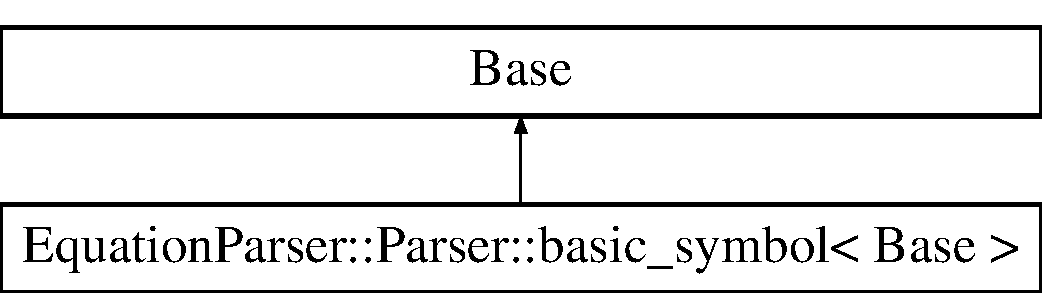
\includegraphics[height=2.000000cm]{structEquationParser_1_1Parser_1_1basic__symbol}
\end{center}
\end{figure}
\subsection*{Public Types}
\begin{DoxyCompactItemize}
\item 
typedef Base \hyperlink{structEquationParser_1_1Parser_1_1basic__symbol_a7ffb114bfe6a321069bbd6baeaefa0f7}{super\+\_\+type}\hypertarget{structEquationParser_1_1Parser_1_1basic__symbol_a7ffb114bfe6a321069bbd6baeaefa0f7}{}\label{structEquationParser_1_1Parser_1_1basic__symbol_a7ffb114bfe6a321069bbd6baeaefa0f7}

\begin{DoxyCompactList}\small\item\em Alias to Base. \end{DoxyCompactList}\end{DoxyCompactItemize}
\subsection*{Public Member Functions}
\begin{DoxyCompactItemize}
\item 
\hyperlink{structEquationParser_1_1Parser_1_1basic__symbol_a7cc26057f5a4fe2232f39c0880ccab0c}{basic\+\_\+symbol} ()\hypertarget{structEquationParser_1_1Parser_1_1basic__symbol_a7cc26057f5a4fe2232f39c0880ccab0c}{}\label{structEquationParser_1_1Parser_1_1basic__symbol_a7cc26057f5a4fe2232f39c0880ccab0c}

\begin{DoxyCompactList}\small\item\em Default constructor. \end{DoxyCompactList}\item 
\hyperlink{structEquationParser_1_1Parser_1_1basic__symbol_aa4f69c5693e9d05ef7ce655f2903dd26}{basic\+\_\+symbol} (const \hyperlink{structEquationParser_1_1Parser_1_1basic__symbol}{basic\+\_\+symbol} \&other)\hypertarget{structEquationParser_1_1Parser_1_1basic__symbol_aa4f69c5693e9d05ef7ce655f2903dd26}{}\label{structEquationParser_1_1Parser_1_1basic__symbol_aa4f69c5693e9d05ef7ce655f2903dd26}

\begin{DoxyCompactList}\small\item\em Copy constructor. \end{DoxyCompactList}\item 
\hyperlink{structEquationParser_1_1Parser_1_1basic__symbol_a3fafc195e2a9279615f90d200cdcf007}{basic\+\_\+symbol} (typename Base\+::kind\+\_\+type t, const \hyperlink{classEquationParser_1_1Parser_a9c08ca33906dfb521b4ec5989e3620bf}{location\+\_\+type} \&l)\hypertarget{structEquationParser_1_1Parser_1_1basic__symbol_a3fafc195e2a9279615f90d200cdcf007}{}\label{structEquationParser_1_1Parser_1_1basic__symbol_a3fafc195e2a9279615f90d200cdcf007}

\begin{DoxyCompactList}\small\item\em Constructor for valueless symbols, and symbols from each type. \end{DoxyCompactList}\item 
{\bfseries basic\+\_\+symbol} (typename Base\+::kind\+\_\+type t, const class \hyperlink{classCalculationNode}{Calculation\+Node} $\ast$v, const \hyperlink{classEquationParser_1_1Parser_a9c08ca33906dfb521b4ec5989e3620bf}{location\+\_\+type} \&l)\hypertarget{structEquationParser_1_1Parser_1_1basic__symbol_ade1fd985fd00a788ecd9b38247a5681b}{}\label{structEquationParser_1_1Parser_1_1basic__symbol_ade1fd985fd00a788ecd9b38247a5681b}

\item 
{\bfseries basic\+\_\+symbol} (typename Base\+::kind\+\_\+type t, const double v, const \hyperlink{classEquationParser_1_1Parser_a9c08ca33906dfb521b4ec5989e3620bf}{location\+\_\+type} \&l)\hypertarget{structEquationParser_1_1Parser_1_1basic__symbol_a2a3e48955c45f4c130876769901bf8e0}{}\label{structEquationParser_1_1Parser_1_1basic__symbol_a2a3e48955c45f4c130876769901bf8e0}

\item 
{\bfseries basic\+\_\+symbol} (typename Base\+::kind\+\_\+type t, const int v, const \hyperlink{classEquationParser_1_1Parser_a9c08ca33906dfb521b4ec5989e3620bf}{location\+\_\+type} \&l)\hypertarget{structEquationParser_1_1Parser_1_1basic__symbol_a36ce3f83e22f490b32beb68495e2628e}{}\label{structEquationParser_1_1Parser_1_1basic__symbol_a36ce3f83e22f490b32beb68495e2628e}

\item 
{\bfseries basic\+\_\+symbol} (typename Base\+::kind\+\_\+type t, const std\+::string v, const \hyperlink{classEquationParser_1_1Parser_a9c08ca33906dfb521b4ec5989e3620bf}{location\+\_\+type} \&l)\hypertarget{structEquationParser_1_1Parser_1_1basic__symbol_acd6411a9ab52f90961960e992e91b1a2}{}\label{structEquationParser_1_1Parser_1_1basic__symbol_acd6411a9ab52f90961960e992e91b1a2}

\item 
\hyperlink{structEquationParser_1_1Parser_1_1basic__symbol_aa5293c259d4e6a166a556a0a85bfd613}{basic\+\_\+symbol} (typename Base\+::kind\+\_\+type t, const \hyperlink{classEquationParser_1_1Parser_a86482685d5f3d44fff68fd4150bbd2dd}{semantic\+\_\+type} \&v, const \hyperlink{classEquationParser_1_1Parser_a9c08ca33906dfb521b4ec5989e3620bf}{location\+\_\+type} \&l)\hypertarget{structEquationParser_1_1Parser_1_1basic__symbol_aa5293c259d4e6a166a556a0a85bfd613}{}\label{structEquationParser_1_1Parser_1_1basic__symbol_aa5293c259d4e6a166a556a0a85bfd613}

\begin{DoxyCompactList}\small\item\em Constructor for symbols with semantic value. \end{DoxyCompactList}\item 
\hyperlink{structEquationParser_1_1Parser_1_1basic__symbol_adecad196c1e623614f818d540ff626c3}{$\sim$basic\+\_\+symbol} ()\hypertarget{structEquationParser_1_1Parser_1_1basic__symbol_adecad196c1e623614f818d540ff626c3}{}\label{structEquationParser_1_1Parser_1_1basic__symbol_adecad196c1e623614f818d540ff626c3}

\begin{DoxyCompactList}\small\item\em Destroy the symbol. \end{DoxyCompactList}\item 
void \hyperlink{structEquationParser_1_1Parser_1_1basic__symbol_a65fcb2cc134131325bef8088e2e34fff}{clear} ()\hypertarget{structEquationParser_1_1Parser_1_1basic__symbol_a65fcb2cc134131325bef8088e2e34fff}{}\label{structEquationParser_1_1Parser_1_1basic__symbol_a65fcb2cc134131325bef8088e2e34fff}

\begin{DoxyCompactList}\small\item\em Destroy contents, and record that is empty. \end{DoxyCompactList}\item 
bool \hyperlink{structEquationParser_1_1Parser_1_1basic__symbol_a3a903eee8a6d93b1e3f0974c509b5f1c}{empty} () const \hypertarget{structEquationParser_1_1Parser_1_1basic__symbol_a3a903eee8a6d93b1e3f0974c509b5f1c}{}\label{structEquationParser_1_1Parser_1_1basic__symbol_a3a903eee8a6d93b1e3f0974c509b5f1c}

\begin{DoxyCompactList}\small\item\em Whether empty. \end{DoxyCompactList}\item 
void \hyperlink{structEquationParser_1_1Parser_1_1basic__symbol_aa7a18dbff0460730c89ad5718263299d}{move} (\hyperlink{structEquationParser_1_1Parser_1_1basic__symbol}{basic\+\_\+symbol} \&s)\hypertarget{structEquationParser_1_1Parser_1_1basic__symbol_aa7a18dbff0460730c89ad5718263299d}{}\label{structEquationParser_1_1Parser_1_1basic__symbol_aa7a18dbff0460730c89ad5718263299d}

\begin{DoxyCompactList}\small\item\em Destructive move, {\itshape s} is emptied into this. \end{DoxyCompactList}\end{DoxyCompactItemize}
\subsection*{Public Attributes}
\begin{DoxyCompactItemize}
\item 
\hyperlink{classEquationParser_1_1Parser_a86482685d5f3d44fff68fd4150bbd2dd}{semantic\+\_\+type} \hyperlink{structEquationParser_1_1Parser_1_1basic__symbol_af1042675e7012ce74eb1c18963c2ecd8}{value}\hypertarget{structEquationParser_1_1Parser_1_1basic__symbol_af1042675e7012ce74eb1c18963c2ecd8}{}\label{structEquationParser_1_1Parser_1_1basic__symbol_af1042675e7012ce74eb1c18963c2ecd8}

\begin{DoxyCompactList}\small\item\em The semantic value. \end{DoxyCompactList}\item 
\hyperlink{classEquationParser_1_1Parser_a9c08ca33906dfb521b4ec5989e3620bf}{location\+\_\+type} \hyperlink{structEquationParser_1_1Parser_1_1basic__symbol_a0c1ce0a22bce2efd038930916a006243}{location}\hypertarget{structEquationParser_1_1Parser_1_1basic__symbol_a0c1ce0a22bce2efd038930916a006243}{}\label{structEquationParser_1_1Parser_1_1basic__symbol_a0c1ce0a22bce2efd038930916a006243}

\begin{DoxyCompactList}\small\item\em The location. \end{DoxyCompactList}\end{DoxyCompactItemize}


\subsection{Detailed Description}
\subsubsection*{template$<$typename Base$>$\\*
struct Equation\+Parser\+::\+Parser\+::basic\+\_\+symbol$<$ Base $>$}

A complete symbol.

Expects its Base type to provide access to the symbol type via type\+\_\+get().

Provide access to semantic value and location. 

The documentation for this struct was generated from the following file\+:\begin{DoxyCompactItemize}
\item 
/home/mate/\+Documents/\+Programming/\+Research/\+Multilayer\+Network\+Model/\+Multilayer\+Network\+Model/src/parser/include/\hyperlink{parser_8hpp}{parser.\+hpp}\end{DoxyCompactItemize}

\hypertarget{classBasicIStreamWrapper}{}\section{Basic\+I\+Stream\+Wrapper$<$ Stream\+Type $>$ Class Template Reference}
\label{classBasicIStreamWrapper}\index{Basic\+I\+Stream\+Wrapper$<$ Stream\+Type $>$@{Basic\+I\+Stream\+Wrapper$<$ Stream\+Type $>$}}


Wrapper of {\ttfamily std\+::basic\+\_\+istream} into Rapid\+J\+S\+ON\textquotesingle{}s Stream concept.  




{\ttfamily \#include $<$istreamwrapper.\+h$>$}

\subsection*{Public Types}
\begin{DoxyCompactItemize}
\item 
typedef Stream\+Type\+::char\+\_\+type {\bfseries Ch}\hypertarget{classBasicIStreamWrapper_a88e4288ecdaa0d31ddf4e5917b9aa8d7}{}\label{classBasicIStreamWrapper_a88e4288ecdaa0d31ddf4e5917b9aa8d7}

\end{DoxyCompactItemize}
\subsection*{Public Member Functions}
\begin{DoxyCompactItemize}
\item 
{\bfseries Basic\+I\+Stream\+Wrapper} (Stream\+Type \&stream)\hypertarget{classBasicIStreamWrapper_a3e9a2dd2b6b28243f8f2a911f67cdf56}{}\label{classBasicIStreamWrapper_a3e9a2dd2b6b28243f8f2a911f67cdf56}

\item 
Ch {\bfseries Peek} () const \hypertarget{classBasicIStreamWrapper_ae0c3f22e0955034c3dc90c2398ff4742}{}\label{classBasicIStreamWrapper_ae0c3f22e0955034c3dc90c2398ff4742}

\item 
Ch {\bfseries Take} ()\hypertarget{classBasicIStreamWrapper_afb71f0329d0abbbc9b22ebeb5c1464d1}{}\label{classBasicIStreamWrapper_afb71f0329d0abbbc9b22ebeb5c1464d1}

\item 
size\+\_\+t {\bfseries Tell} () const \hypertarget{classBasicIStreamWrapper_a7da87efb1177bfaa131f33c0cb2873fc}{}\label{classBasicIStreamWrapper_a7da87efb1177bfaa131f33c0cb2873fc}

\item 
Ch $\ast$ {\bfseries Put\+Begin} ()\hypertarget{classBasicIStreamWrapper_a62a3fc10b009ea231fb9d2dc958c539c}{}\label{classBasicIStreamWrapper_a62a3fc10b009ea231fb9d2dc958c539c}

\item 
void {\bfseries Put} (Ch)\hypertarget{classBasicIStreamWrapper_afa71cb2f5b7668837d0a81e3bce55e69}{}\label{classBasicIStreamWrapper_afa71cb2f5b7668837d0a81e3bce55e69}

\item 
void {\bfseries Flush} ()\hypertarget{classBasicIStreamWrapper_a37d5e4cd8fdf3c83dad50737e95886a9}{}\label{classBasicIStreamWrapper_a37d5e4cd8fdf3c83dad50737e95886a9}

\item 
size\+\_\+t {\bfseries Put\+End} (Ch $\ast$)\hypertarget{classBasicIStreamWrapper_ab2ead53490207a1cb0bdd674a03957f3}{}\label{classBasicIStreamWrapper_ab2ead53490207a1cb0bdd674a03957f3}

\item 
const Ch $\ast$ {\bfseries Peek4} () const \hypertarget{classBasicIStreamWrapper_aaae0c7e7f2d06eb1638cce33ed664f31}{}\label{classBasicIStreamWrapper_aaae0c7e7f2d06eb1638cce33ed664f31}

\end{DoxyCompactItemize}


\subsection{Detailed Description}
\subsubsection*{template$<$typename Stream\+Type$>$\\*
class Basic\+I\+Stream\+Wrapper$<$ Stream\+Type $>$}

Wrapper of {\ttfamily std\+::basic\+\_\+istream} into Rapid\+J\+S\+ON\textquotesingle{}s Stream concept. 

The classes can be wrapped including but not limited to\+:


\begin{DoxyItemize}
\item {\ttfamily std\+::istringstream} 
\item {\ttfamily std\+::stringstream} 
\item {\ttfamily std\+::wistringstream} 
\item {\ttfamily std\+::wstringstream} 
\item {\ttfamily std\+::ifstream} 
\item {\ttfamily std\+::fstream} 
\item {\ttfamily std\+::wifstream} 
\item {\ttfamily std\+::wfstream} 
\end{DoxyItemize}


\begin{DoxyTemplParams}{Template Parameters}
{\em Stream\+Type} & Class derived from {\ttfamily std\+::basic\+\_\+istream}. \\
\hline
\end{DoxyTemplParams}


The documentation for this class was generated from the following file\+:\begin{DoxyCompactItemize}
\item 
/home/mate/\+Documents/\+Programming/\+Research/\+Multilayer\+Network\+Model/\+Multilayer\+Network\+Model/sources/external/rapidjson/istreamwrapper.\+h\end{DoxyCompactItemize}

\hypertarget{classBasicOStreamWrapper}{}\section{Basic\+O\+Stream\+Wrapper$<$ Stream\+Type $>$ Class Template Reference}
\label{classBasicOStreamWrapper}\index{Basic\+O\+Stream\+Wrapper$<$ Stream\+Type $>$@{Basic\+O\+Stream\+Wrapper$<$ Stream\+Type $>$}}


Wrapper of {\ttfamily std\+::basic\+\_\+ostream} into Rapid\+J\+S\+ON\textquotesingle{}s Stream concept.  




{\ttfamily \#include $<$ostreamwrapper.\+h$>$}

\subsection*{Public Types}
\begin{DoxyCompactItemize}
\item 
typedef Stream\+Type\+::char\+\_\+type {\bfseries Ch}\hypertarget{classBasicOStreamWrapper_aafc6276f1f5cc0b8d45d137584d380bb}{}\label{classBasicOStreamWrapper_aafc6276f1f5cc0b8d45d137584d380bb}

\end{DoxyCompactItemize}
\subsection*{Public Member Functions}
\begin{DoxyCompactItemize}
\item 
{\bfseries Basic\+O\+Stream\+Wrapper} (Stream\+Type \&stream)\hypertarget{classBasicOStreamWrapper_a067a516c13b7c9d4dacef598d32779ef}{}\label{classBasicOStreamWrapper_a067a516c13b7c9d4dacef598d32779ef}

\item 
void {\bfseries Put} (Ch c)\hypertarget{classBasicOStreamWrapper_a7d3ba9d651fbe27fe05387f512154ea8}{}\label{classBasicOStreamWrapper_a7d3ba9d651fbe27fe05387f512154ea8}

\item 
void {\bfseries Flush} ()\hypertarget{classBasicOStreamWrapper_a1c48a8b7520b0ab6ca34e665b928b56d}{}\label{classBasicOStreamWrapper_a1c48a8b7520b0ab6ca34e665b928b56d}

\item 
char {\bfseries Peek} () const \hypertarget{classBasicOStreamWrapper_a81eda65252d99c350d754bb702526dae}{}\label{classBasicOStreamWrapper_a81eda65252d99c350d754bb702526dae}

\item 
char {\bfseries Take} ()\hypertarget{classBasicOStreamWrapper_a54be63e8d24f4d82329b860a907f65fe}{}\label{classBasicOStreamWrapper_a54be63e8d24f4d82329b860a907f65fe}

\item 
size\+\_\+t {\bfseries Tell} () const \hypertarget{classBasicOStreamWrapper_ab5f119855c8591b650fbcbeb99be677e}{}\label{classBasicOStreamWrapper_ab5f119855c8591b650fbcbeb99be677e}

\item 
char $\ast$ {\bfseries Put\+Begin} ()\hypertarget{classBasicOStreamWrapper_a564b7b727bdab12185e7a7bd1ac5e822}{}\label{classBasicOStreamWrapper_a564b7b727bdab12185e7a7bd1ac5e822}

\item 
size\+\_\+t {\bfseries Put\+End} (char $\ast$)\hypertarget{classBasicOStreamWrapper_a1da108e43a5a517c4484821fced1fca0}{}\label{classBasicOStreamWrapper_a1da108e43a5a517c4484821fced1fca0}

\end{DoxyCompactItemize}


\subsection{Detailed Description}
\subsubsection*{template$<$typename Stream\+Type$>$\\*
class Basic\+O\+Stream\+Wrapper$<$ Stream\+Type $>$}

Wrapper of {\ttfamily std\+::basic\+\_\+ostream} into Rapid\+J\+S\+ON\textquotesingle{}s Stream concept. 

The classes can be wrapped including but not limited to\+:


\begin{DoxyItemize}
\item {\ttfamily std\+::ostringstream} 
\item {\ttfamily std\+::stringstream} 
\item {\ttfamily std\+::wpstringstream} 
\item {\ttfamily std\+::wstringstream} 
\item {\ttfamily std\+::ifstream} 
\item {\ttfamily std\+::fstream} 
\item {\ttfamily std\+::wofstream} 
\item {\ttfamily std\+::wfstream} 
\end{DoxyItemize}


\begin{DoxyTemplParams}{Template Parameters}
{\em Stream\+Type} & Class derived from {\ttfamily std\+::basic\+\_\+ostream}. \\
\hline
\end{DoxyTemplParams}


The documentation for this class was generated from the following file\+:\begin{DoxyCompactItemize}
\item 
/home/mate/\+Documents/\+Programming/\+Research/\+Multilayer\+Network\+Model/\+Multilayer\+Network\+Model/sources/external/rapidjson/ostreamwrapper.\+h\end{DoxyCompactItemize}

\hypertarget{classinternal_1_1BigInteger}{}\section{internal\+:\+:Big\+Integer Class Reference}
\label{classinternal_1_1BigInteger}\index{internal\+::\+Big\+Integer@{internal\+::\+Big\+Integer}}
\subsection*{Public Types}
\begin{DoxyCompactItemize}
\item 
typedef uint64\+\_\+t {\bfseries Type}\hypertarget{classinternal_1_1BigInteger_a1310812fca26ebae77594ba08678fc4c}{}\label{classinternal_1_1BigInteger_a1310812fca26ebae77594ba08678fc4c}

\end{DoxyCompactItemize}
\subsection*{Public Member Functions}
\begin{DoxyCompactItemize}
\item 
{\bfseries Big\+Integer} (const \hyperlink{classinternal_1_1BigInteger}{Big\+Integer} \&rhs)\hypertarget{classinternal_1_1BigInteger_abec623168bc9494dec2f50643b897f72}{}\label{classinternal_1_1BigInteger_abec623168bc9494dec2f50643b897f72}

\item 
{\bfseries Big\+Integer} (uint64\+\_\+t u)\hypertarget{classinternal_1_1BigInteger_ad02b0ef9da203efddd4af07e923732c0}{}\label{classinternal_1_1BigInteger_ad02b0ef9da203efddd4af07e923732c0}

\item 
{\bfseries Big\+Integer} (const char $\ast$decimals, size\+\_\+t length)\hypertarget{classinternal_1_1BigInteger_a656bd1bd4af3920beb90ba4af87b6181}{}\label{classinternal_1_1BigInteger_a656bd1bd4af3920beb90ba4af87b6181}

\item 
\hyperlink{classinternal_1_1BigInteger}{Big\+Integer} \& {\bfseries operator=} (const \hyperlink{classinternal_1_1BigInteger}{Big\+Integer} \&rhs)\hypertarget{classinternal_1_1BigInteger_ae3eaf1b96cd993511c9f48a14dfc3af2}{}\label{classinternal_1_1BigInteger_ae3eaf1b96cd993511c9f48a14dfc3af2}

\item 
\hyperlink{classinternal_1_1BigInteger}{Big\+Integer} \& {\bfseries operator=} (uint64\+\_\+t u)\hypertarget{classinternal_1_1BigInteger_a4002e0b1cf5ee68ab94ab65b35167a38}{}\label{classinternal_1_1BigInteger_a4002e0b1cf5ee68ab94ab65b35167a38}

\item 
\hyperlink{classinternal_1_1BigInteger}{Big\+Integer} \& {\bfseries operator+=} (uint64\+\_\+t u)\hypertarget{classinternal_1_1BigInteger_a09af1d6658d51ad4372649ce1c9c1a62}{}\label{classinternal_1_1BigInteger_a09af1d6658d51ad4372649ce1c9c1a62}

\item 
\hyperlink{classinternal_1_1BigInteger}{Big\+Integer} \& {\bfseries operator$\ast$=} (uint64\+\_\+t u)\hypertarget{classinternal_1_1BigInteger_a79a52c6135c9783f2e53432dce2cde89}{}\label{classinternal_1_1BigInteger_a79a52c6135c9783f2e53432dce2cde89}

\item 
\hyperlink{classinternal_1_1BigInteger}{Big\+Integer} \& {\bfseries operator$\ast$=} (uint32\+\_\+t u)\hypertarget{classinternal_1_1BigInteger_a83e8e464b7bc31c8b2c943f8563b2226}{}\label{classinternal_1_1BigInteger_a83e8e464b7bc31c8b2c943f8563b2226}

\item 
\hyperlink{classinternal_1_1BigInteger}{Big\+Integer} \& {\bfseries operator$<$$<$=} (size\+\_\+t shift)\hypertarget{classinternal_1_1BigInteger_a48b12ef4676f19290dfd5816a4ef4a88}{}\label{classinternal_1_1BigInteger_a48b12ef4676f19290dfd5816a4ef4a88}

\item 
bool {\bfseries operator==} (const \hyperlink{classinternal_1_1BigInteger}{Big\+Integer} \&rhs) const \hypertarget{classinternal_1_1BigInteger_a567ecda3009de20400a2af649fb87e60}{}\label{classinternal_1_1BigInteger_a567ecda3009de20400a2af649fb87e60}

\item 
bool {\bfseries operator==} (const Type rhs) const \hypertarget{classinternal_1_1BigInteger_a329eddac1b724f82d56af2ee2c8abcc4}{}\label{classinternal_1_1BigInteger_a329eddac1b724f82d56af2ee2c8abcc4}

\item 
\hyperlink{classinternal_1_1BigInteger}{Big\+Integer} \& {\bfseries Multiply\+Pow5} (unsigned exp)\hypertarget{classinternal_1_1BigInteger_a98a13f169c27d1acfa57054f37c61763}{}\label{classinternal_1_1BigInteger_a98a13f169c27d1acfa57054f37c61763}

\item 
bool {\bfseries Difference} (const \hyperlink{classinternal_1_1BigInteger}{Big\+Integer} \&rhs, \hyperlink{classinternal_1_1BigInteger}{Big\+Integer} $\ast$out) const \hypertarget{classinternal_1_1BigInteger_a5741304ce36392adeef716e78b384b61}{}\label{classinternal_1_1BigInteger_a5741304ce36392adeef716e78b384b61}

\item 
int {\bfseries Compare} (const \hyperlink{classinternal_1_1BigInteger}{Big\+Integer} \&rhs) const \hypertarget{classinternal_1_1BigInteger_afd8b15480df5003ee6b6e1b8ecbf5f45}{}\label{classinternal_1_1BigInteger_afd8b15480df5003ee6b6e1b8ecbf5f45}

\item 
size\+\_\+t {\bfseries Get\+Count} () const \hypertarget{classinternal_1_1BigInteger_a720114cef0871c9f9c3c6a5f3a66e66a}{}\label{classinternal_1_1BigInteger_a720114cef0871c9f9c3c6a5f3a66e66a}

\item 
Type {\bfseries Get\+Digit} (size\+\_\+t index) const \hypertarget{classinternal_1_1BigInteger_a92c6854f2388875374cfb9801bea0cc8}{}\label{classinternal_1_1BigInteger_a92c6854f2388875374cfb9801bea0cc8}

\item 
bool {\bfseries Is\+Zero} () const \hypertarget{classinternal_1_1BigInteger_a99cf9cb87491a583c6b7614b0c8654fe}{}\label{classinternal_1_1BigInteger_a99cf9cb87491a583c6b7614b0c8654fe}

\end{DoxyCompactItemize}


The documentation for this class was generated from the following file\+:\begin{DoxyCompactItemize}
\item 
/home/mate/\+Documents/\+Programming/\+Research/\+Multilayer\+Network\+Model/\+Multilayer\+Network\+Model/src/external/rapidjson/internal/biginteger.\+h\end{DoxyCompactItemize}

\hypertarget{structEquationParser_1_1Parser_1_1by__type}{}\section{Equation\+Parser\+:\+:Parser\+:\+:by\+\_\+type Struct Reference}
\label{structEquationParser_1_1Parser_1_1by__type}\index{Equation\+Parser\+::\+Parser\+::by\+\_\+type@{Equation\+Parser\+::\+Parser\+::by\+\_\+type}}


Type access provider for token (enum) based symbols.  




{\ttfamily \#include $<$parser.\+hpp$>$}

\subsection*{Public Types}
\begin{DoxyCompactItemize}
\item 
typedef \hyperlink{classEquationParser_1_1Parser_aa29d1fb4fbd9ec112dcb2acd504dc2f1}{token\+\_\+type} \hyperlink{structEquationParser_1_1Parser_1_1by__type_af198f005fea2f0213fff81e59c3d2635}{kind\+\_\+type}\hypertarget{structEquationParser_1_1Parser_1_1by__type_af198f005fea2f0213fff81e59c3d2635}{}\label{structEquationParser_1_1Parser_1_1by__type_af198f005fea2f0213fff81e59c3d2635}

\begin{DoxyCompactList}\small\item\em The symbol type as needed by the constructor. \end{DoxyCompactList}\end{DoxyCompactItemize}
\subsection*{Public Member Functions}
\begin{DoxyCompactItemize}
\item 
\hyperlink{structEquationParser_1_1Parser_1_1by__type_a80e5b1a5f15c93b21587aacf99ea6683}{by\+\_\+type} ()\hypertarget{structEquationParser_1_1Parser_1_1by__type_a80e5b1a5f15c93b21587aacf99ea6683}{}\label{structEquationParser_1_1Parser_1_1by__type_a80e5b1a5f15c93b21587aacf99ea6683}

\begin{DoxyCompactList}\small\item\em Default constructor. \end{DoxyCompactList}\item 
\hyperlink{structEquationParser_1_1Parser_1_1by__type_aea5fa9e6d75e898e034fd355f46a9ecf}{by\+\_\+type} (const \hyperlink{structEquationParser_1_1Parser_1_1by__type}{by\+\_\+type} \&other)\hypertarget{structEquationParser_1_1Parser_1_1by__type_aea5fa9e6d75e898e034fd355f46a9ecf}{}\label{structEquationParser_1_1Parser_1_1by__type_aea5fa9e6d75e898e034fd355f46a9ecf}

\begin{DoxyCompactList}\small\item\em Copy constructor. \end{DoxyCompactList}\item 
\hyperlink{structEquationParser_1_1Parser_1_1by__type_ad56c4f12102f4f3531ebc166d3e773ee}{by\+\_\+type} (\hyperlink{structEquationParser_1_1Parser_1_1by__type_af198f005fea2f0213fff81e59c3d2635}{kind\+\_\+type} t)\hypertarget{structEquationParser_1_1Parser_1_1by__type_ad56c4f12102f4f3531ebc166d3e773ee}{}\label{structEquationParser_1_1Parser_1_1by__type_ad56c4f12102f4f3531ebc166d3e773ee}

\begin{DoxyCompactList}\small\item\em Constructor from (external) token numbers. \end{DoxyCompactList}\item 
void \hyperlink{structEquationParser_1_1Parser_1_1by__type_ad3bb04dfea2662229852171462c013ea}{clear} ()\hypertarget{structEquationParser_1_1Parser_1_1by__type_ad3bb04dfea2662229852171462c013ea}{}\label{structEquationParser_1_1Parser_1_1by__type_ad3bb04dfea2662229852171462c013ea}

\begin{DoxyCompactList}\small\item\em Record that this symbol is empty. \end{DoxyCompactList}\item 
void \hyperlink{structEquationParser_1_1Parser_1_1by__type_a7a9811cc1ede6a822191ae3bba1014bc}{move} (\hyperlink{structEquationParser_1_1Parser_1_1by__type}{by\+\_\+type} \&that)\hypertarget{structEquationParser_1_1Parser_1_1by__type_a7a9811cc1ede6a822191ae3bba1014bc}{}\label{structEquationParser_1_1Parser_1_1by__type_a7a9811cc1ede6a822191ae3bba1014bc}

\begin{DoxyCompactList}\small\item\em Steal the symbol type from {\itshape that}. \end{DoxyCompactList}\item 
\hyperlink{classEquationParser_1_1Parser_a95a5093ff65178baa4926eebed7aacf0}{symbol\+\_\+number\+\_\+type} \hyperlink{structEquationParser_1_1Parser_1_1by__type_a7b4d1f64d58bd690ea167072746a5c20}{type\+\_\+get} () const 
\item 
\hyperlink{classEquationParser_1_1Parser_aa29d1fb4fbd9ec112dcb2acd504dc2f1}{token\+\_\+type} \hyperlink{structEquationParser_1_1Parser_1_1by__type_ae546ecc7c21fa45110ab4b0ca59d3d3d}{token} () const \hypertarget{structEquationParser_1_1Parser_1_1by__type_ae546ecc7c21fa45110ab4b0ca59d3d3d}{}\label{structEquationParser_1_1Parser_1_1by__type_ae546ecc7c21fa45110ab4b0ca59d3d3d}

\begin{DoxyCompactList}\small\item\em The token. \end{DoxyCompactList}\end{DoxyCompactItemize}
\subsection*{Public Attributes}
\begin{DoxyCompactItemize}
\item 
int \hyperlink{structEquationParser_1_1Parser_1_1by__type_af116c7ee695735c0b9a2a6e74efa25f0}{type}
\end{DoxyCompactItemize}


\subsection{Detailed Description}
Type access provider for token (enum) based symbols. 

\subsection{Member Function Documentation}
\index{Equation\+Parser\+::\+Parser\+::by\+\_\+type@{Equation\+Parser\+::\+Parser\+::by\+\_\+type}!type\+\_\+get@{type\+\_\+get}}
\index{type\+\_\+get@{type\+\_\+get}!Equation\+Parser\+::\+Parser\+::by\+\_\+type@{Equation\+Parser\+::\+Parser\+::by\+\_\+type}}
\subsubsection[{\texorpdfstring{type\+\_\+get() const }{type_get() const }}]{\setlength{\rightskip}{0pt plus 5cm}int Equation\+Parser\+::\+Parser\+::by\+\_\+type\+::type\+\_\+get (
\begin{DoxyParamCaption}
{}
\end{DoxyParamCaption}
) const\hspace{0.3cm}{\ttfamily [inline]}}\hypertarget{structEquationParser_1_1Parser_1_1by__type_a7b4d1f64d58bd690ea167072746a5c20}{}\label{structEquationParser_1_1Parser_1_1by__type_a7b4d1f64d58bd690ea167072746a5c20}
The (internal) type number (corresponding to {\itshape type}). {\itshape empty} when empty. 

\subsection{Member Data Documentation}
\index{Equation\+Parser\+::\+Parser\+::by\+\_\+type@{Equation\+Parser\+::\+Parser\+::by\+\_\+type}!type@{type}}
\index{type@{type}!Equation\+Parser\+::\+Parser\+::by\+\_\+type@{Equation\+Parser\+::\+Parser\+::by\+\_\+type}}
\subsubsection[{\texorpdfstring{type}{type}}]{\setlength{\rightskip}{0pt plus 5cm}int Equation\+Parser\+::\+Parser\+::by\+\_\+type\+::type}\hypertarget{structEquationParser_1_1Parser_1_1by__type_af116c7ee695735c0b9a2a6e74efa25f0}{}\label{structEquationParser_1_1Parser_1_1by__type_af116c7ee695735c0b9a2a6e74efa25f0}
The symbol type. {\itshape empty\+\_\+symbol} when empty. An int, not token\+\_\+number\+\_\+type, to be able to store empty\+\_\+symbol. 

The documentation for this struct was generated from the following file\+:\begin{DoxyCompactItemize}
\item 
/home/mate/\+Documents/\+Programming/\+Research/\+Multilayer\+Network\+Model/\+Multilayer\+Network\+Model/src/parser/include/\hyperlink{parser_8hpp}{parser.\+hpp}\end{DoxyCompactItemize}

\hypertarget{classCalculationNode}{}\section{Calculation\+Node Class Reference}
\label{classCalculationNode}\index{Calculation\+Node@{Calculation\+Node}}
Inheritance diagram for Calculation\+Node\+:\begin{figure}[H]
\begin{center}
\leavevmode
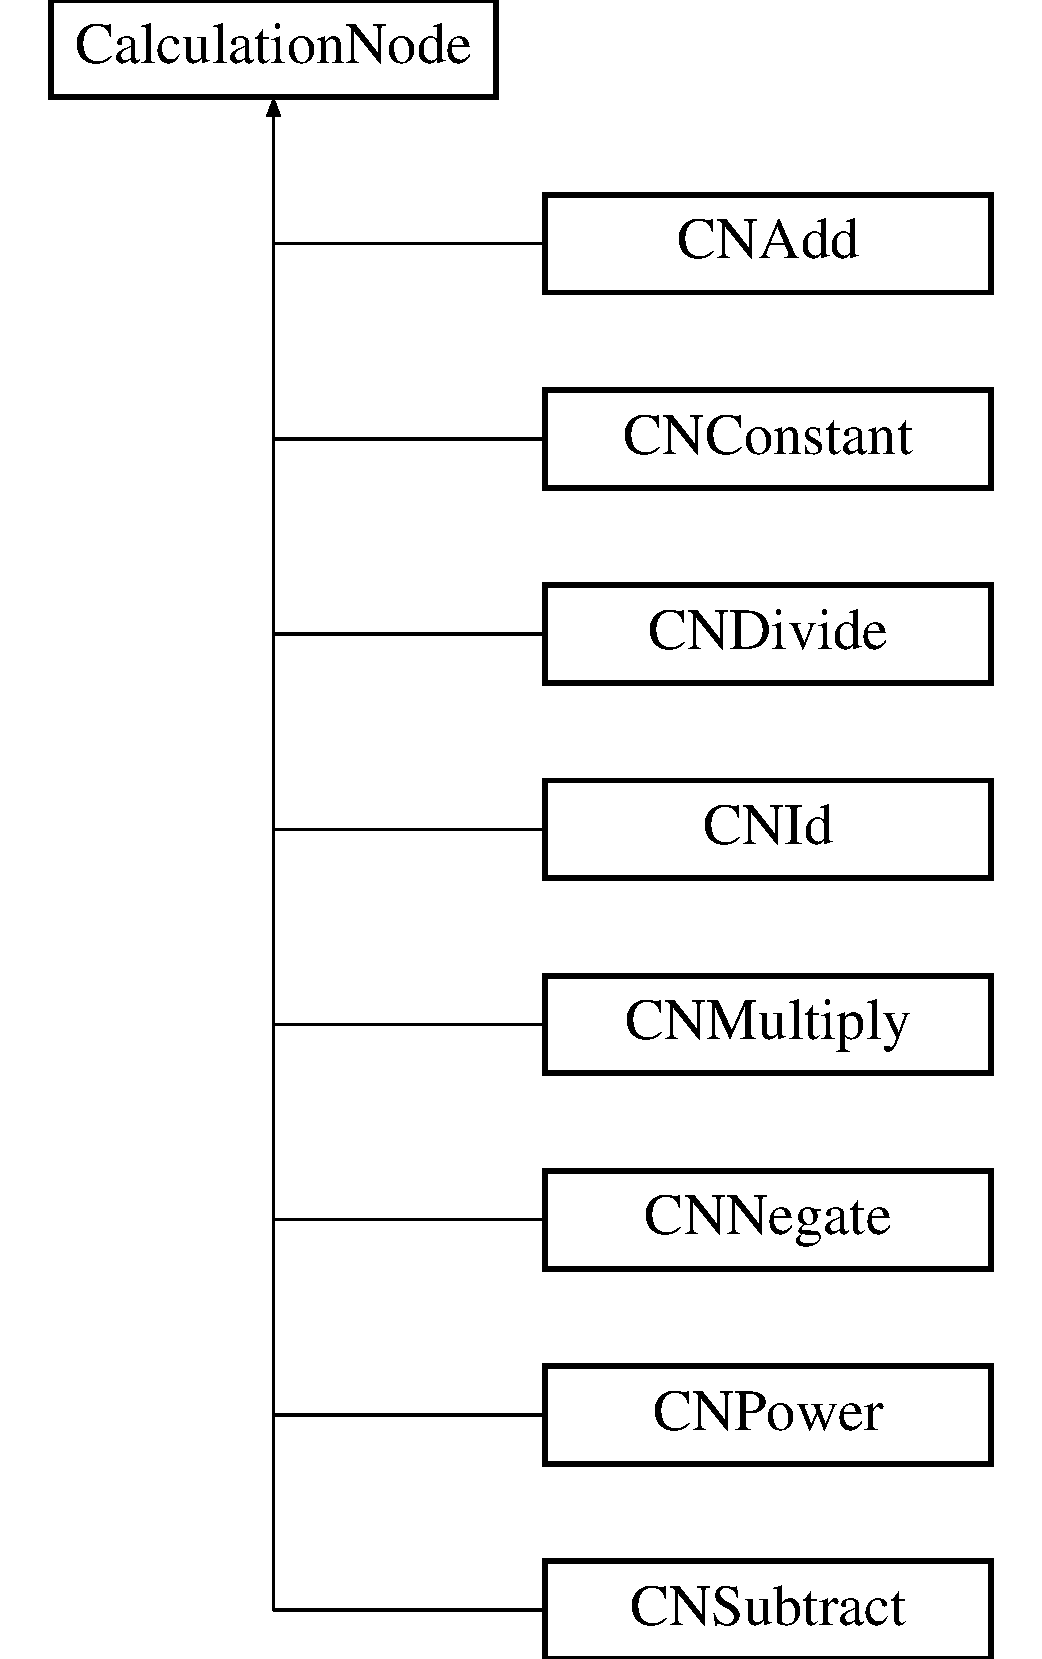
\includegraphics[height=9.000000cm]{classCalculationNode}
\end{center}
\end{figure}
\subsection*{Public Member Functions}
\begin{DoxyCompactItemize}
\item 
virtual double {\bfseries evaluate} () const  =0\hypertarget{classCalculationNode_ac0b4e69fc8bfc99b0ad178b4eeb15883}{}\label{classCalculationNode_ac0b4e69fc8bfc99b0ad178b4eeb15883}

\item 
virtual double {\bfseries evaluate\+At\+State} (std\+::map$<$ int, double $>$) const  =0\hypertarget{classCalculationNode_a15efb576650532bbf21a11f1f9bcb1b2}{}\label{classCalculationNode_a15efb576650532bbf21a11f1f9bcb1b2}

\item 
virtual bool {\bfseries test\+Node\+Ids} () const  =0\hypertarget{classCalculationNode_a4089a2510d7c345a9632843a3fed4f0e}{}\label{classCalculationNode_a4089a2510d7c345a9632843a3fed4f0e}

\item 
virtual std\+::string {\bfseries to\+String} () const  =0\hypertarget{classCalculationNode_aeee8e0d2c7d5c97e0d6801e9644cd686}{}\label{classCalculationNode_aeee8e0d2c7d5c97e0d6801e9644cd686}

\item 
virtual double {\bfseries get\+Value} () const \hypertarget{classCalculationNode_af23ecff57877120eea2f402bb8432549}{}\label{classCalculationNode_af23ecff57877120eea2f402bb8432549}

\item 
virtual void {\bfseries set\+Value} (double value)\hypertarget{classCalculationNode_a63783e44f06e8b665f2f6851616b2965}{}\label{classCalculationNode_a63783e44f06e8b665f2f6851616b2965}

\item 
Calc\+Node\+Types {\bfseries get\+Type} ()\hypertarget{classCalculationNode_ad5df05ec0725d5c4c44b6eecc158a83b}{}\label{classCalculationNode_ad5df05ec0725d5c4c44b6eecc158a83b}

\item 
virtual int {\bfseries get\+Id} ()\hypertarget{classCalculationNode_a57d514437cfc918ddb298d482358c82d}{}\label{classCalculationNode_a57d514437cfc918ddb298d482358c82d}

\item 
virtual void {\bfseries set\+Node} (\hyperlink{classNode}{Node} $\ast$node)\hypertarget{classCalculationNode_a4097a8577ad76d94c32250d76988353c}{}\label{classCalculationNode_a4097a8577ad76d94c32250d76988353c}

\end{DoxyCompactItemize}
\subsection*{Public Attributes}
\begin{DoxyCompactItemize}
\item 
\hyperlink{classCalculationNode}{Calculation\+Node} $\ast$ {\bfseries left}\hypertarget{classCalculationNode_ae82c63d4efc74c0b11a00cc06f225629}{}\label{classCalculationNode_ae82c63d4efc74c0b11a00cc06f225629}

\item 
\hyperlink{classCalculationNode}{Calculation\+Node} $\ast$ {\bfseries right}\hypertarget{classCalculationNode_a55560a0b8fa37b8443c908a06d08f087}{}\label{classCalculationNode_a55560a0b8fa37b8443c908a06d08f087}

\end{DoxyCompactItemize}
\subsection*{Protected Attributes}
\begin{DoxyCompactItemize}
\item 
Calc\+Node\+Types {\bfseries type}\hypertarget{classCalculationNode_a9380df8305abde9a1e3a6a3f5fd6dea0}{}\label{classCalculationNode_a9380df8305abde9a1e3a6a3f5fd6dea0}

\end{DoxyCompactItemize}


The documentation for this class was generated from the following file\+:\begin{DoxyCompactItemize}
\item 
/home/mate/\+Documents/\+Programming/\+Research/\+Multilayer\+Network\+Model/\+Multilayer\+Network\+Model/sources/core/\+Dynamical\+Equation/include/Calculation\+Node.\+hh\end{DoxyCompactItemize}

\hypertarget{classCNAdd}{}\section{C\+N\+Add Class Reference}
\label{classCNAdd}\index{C\+N\+Add@{C\+N\+Add}}
Inheritance diagram for C\+N\+Add\+:\begin{figure}[H]
\begin{center}
\leavevmode
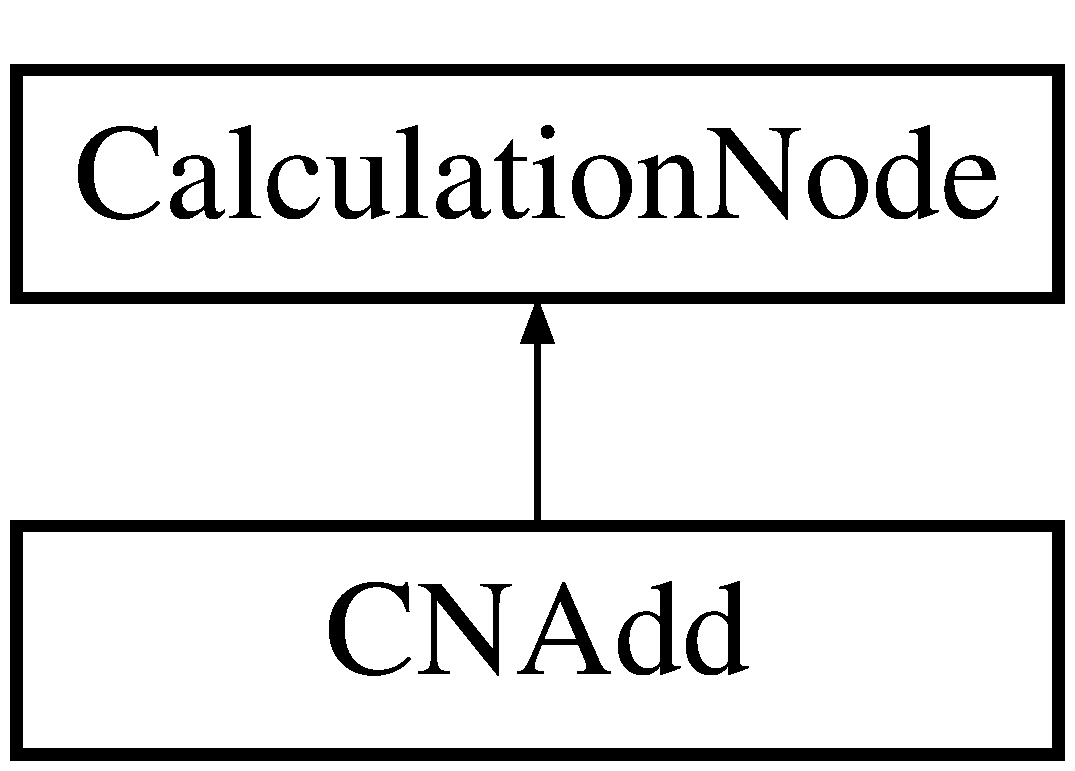
\includegraphics[height=2.000000cm]{classCNAdd}
\end{center}
\end{figure}
\subsection*{Public Member Functions}
\begin{DoxyCompactItemize}
\item 
{\bfseries C\+N\+Add} (\hyperlink{classCalculationNode}{Calculation\+Node} $\ast$\+\_\+left, \hyperlink{classCalculationNode}{Calculation\+Node} $\ast$\+\_\+right)\hypertarget{classCNAdd_a7dab8d6be3e0fa6d804c3593cb1de715}{}\label{classCNAdd_a7dab8d6be3e0fa6d804c3593cb1de715}

\item 
virtual double {\bfseries evaluate} () const \hypertarget{classCNAdd_a5b558f1853ec5555c1ff3503f44b30e7}{}\label{classCNAdd_a5b558f1853ec5555c1ff3503f44b30e7}

\item 
virtual double {\bfseries evaluate\+At\+State} (std\+::map$<$ int, double $>$ starting\+State) const \hypertarget{classCNAdd_a8c4f9b20da9d50fcdd2ac1211da2eee6}{}\label{classCNAdd_a8c4f9b20da9d50fcdd2ac1211da2eee6}

\item 
virtual bool \hyperlink{classCNAdd_a9ded4aa2b5379606d5d110b8cb05ee05}{test\+Node\+Ids} () const 
\item 
virtual std\+::string {\bfseries to\+String} () const \hypertarget{classCNAdd_a6a29c72a161475af0e05361e6cae49cc}{}\label{classCNAdd_a6a29c72a161475af0e05361e6cae49cc}

\end{DoxyCompactItemize}
\subsection*{Additional Inherited Members}


\subsection{Member Function Documentation}
\index{C\+N\+Add@{C\+N\+Add}!test\+Node\+Ids@{test\+Node\+Ids}}
\index{test\+Node\+Ids@{test\+Node\+Ids}!C\+N\+Add@{C\+N\+Add}}
\subsubsection[{\texorpdfstring{test\+Node\+Ids() const }{testNodeIds() const }}]{\setlength{\rightskip}{0pt plus 5cm}virtual bool C\+N\+Add\+::test\+Node\+Ids (
\begin{DoxyParamCaption}
{}
\end{DoxyParamCaption}
) const\hspace{0.3cm}{\ttfamily [inline]}, {\ttfamily [virtual]}}\hypertarget{classCNAdd_a9ded4aa2b5379606d5d110b8cb05ee05}{}\label{classCNAdd_a9ded4aa2b5379606d5d110b8cb05ee05}
Used only for testing puposes. Compared the ID type \hyperlink{classCalculationNode}{Calculation\+Node}\textquotesingle{}s id field to the assigned node\textquotesingle{}s id. 

Implements \hyperlink{classCalculationNode_a4089a2510d7c345a9632843a3fed4f0e}{Calculation\+Node}.



The documentation for this class was generated from the following file\+:\begin{DoxyCompactItemize}
\item 
/home/mate/\+Documents/\+Programming/\+Research/\+Multilayer\+Network\+Model/\+Multilayer\+Network\+Model/sources/core/\+Dynamical\+Equation/include/Calculation\+Node.\+hh\end{DoxyCompactItemize}

\hypertarget{classCNConstant}{}\section{C\+N\+Constant Class Reference}
\label{classCNConstant}\index{C\+N\+Constant@{C\+N\+Constant}}
Inheritance diagram for C\+N\+Constant\+:\begin{figure}[H]
\begin{center}
\leavevmode
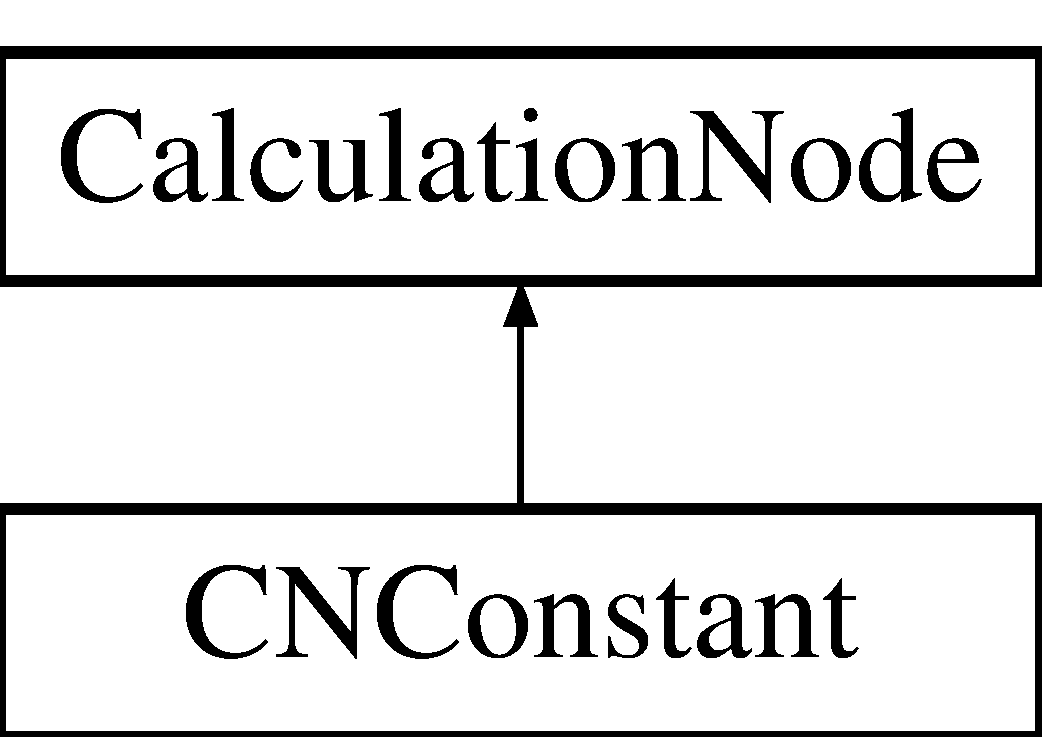
\includegraphics[height=2.000000cm]{classCNConstant}
\end{center}
\end{figure}
\subsection*{Public Member Functions}
\begin{DoxyCompactItemize}
\item 
{\bfseries C\+N\+Constant} (double \+\_\+value)\hypertarget{classCNConstant_a0cf39e7ec935e90a472f8bf4fd784fa2}{}\label{classCNConstant_a0cf39e7ec935e90a472f8bf4fd784fa2}

\item 
virtual double {\bfseries evaluate} () const \hypertarget{classCNConstant_af8f9ed8124c661e1dd31df7e6eed94c3}{}\label{classCNConstant_af8f9ed8124c661e1dd31df7e6eed94c3}

\item 
virtual double {\bfseries evaluate\+At\+State} (std\+::map$<$ int, double $>$ starting\+State) const \hypertarget{classCNConstant_a00d59d4252567658adfc516169645ff5}{}\label{classCNConstant_a00d59d4252567658adfc516169645ff5}

\item 
virtual bool {\bfseries test\+Node\+Ids} () const \hypertarget{classCNConstant_aaa0511d5aa204f30769f2a3a33f78f91}{}\label{classCNConstant_aaa0511d5aa204f30769f2a3a33f78f91}

\item 
virtual std\+::string {\bfseries to\+String} () const \hypertarget{classCNConstant_abd2085b23c5a3502b645068caf53a43f}{}\label{classCNConstant_abd2085b23c5a3502b645068caf53a43f}

\item 
virtual double {\bfseries get\+Value} () const \hypertarget{classCNConstant_ac416282fca8424c0f3d6d65fa2b96f20}{}\label{classCNConstant_ac416282fca8424c0f3d6d65fa2b96f20}

\item 
virtual void {\bfseries set\+Value} (double value)\hypertarget{classCNConstant_a964d75e6934098c33853009a43685a0e}{}\label{classCNConstant_a964d75e6934098c33853009a43685a0e}

\end{DoxyCompactItemize}
\subsection*{Additional Inherited Members}


The documentation for this class was generated from the following file\+:\begin{DoxyCompactItemize}
\item 
/home/mate/\+Documents/\+Programming/\+Research/\+Multilayer\+Network\+Model/\+Multilayer\+Network\+Model/sources/core/\+Dynamical\+Equation/include/Calculation\+Node.\+hh\end{DoxyCompactItemize}

\hypertarget{classCNDivide}{}\section{C\+N\+Divide Class Reference}
\label{classCNDivide}\index{C\+N\+Divide@{C\+N\+Divide}}
Inheritance diagram for C\+N\+Divide\+:\begin{figure}[H]
\begin{center}
\leavevmode
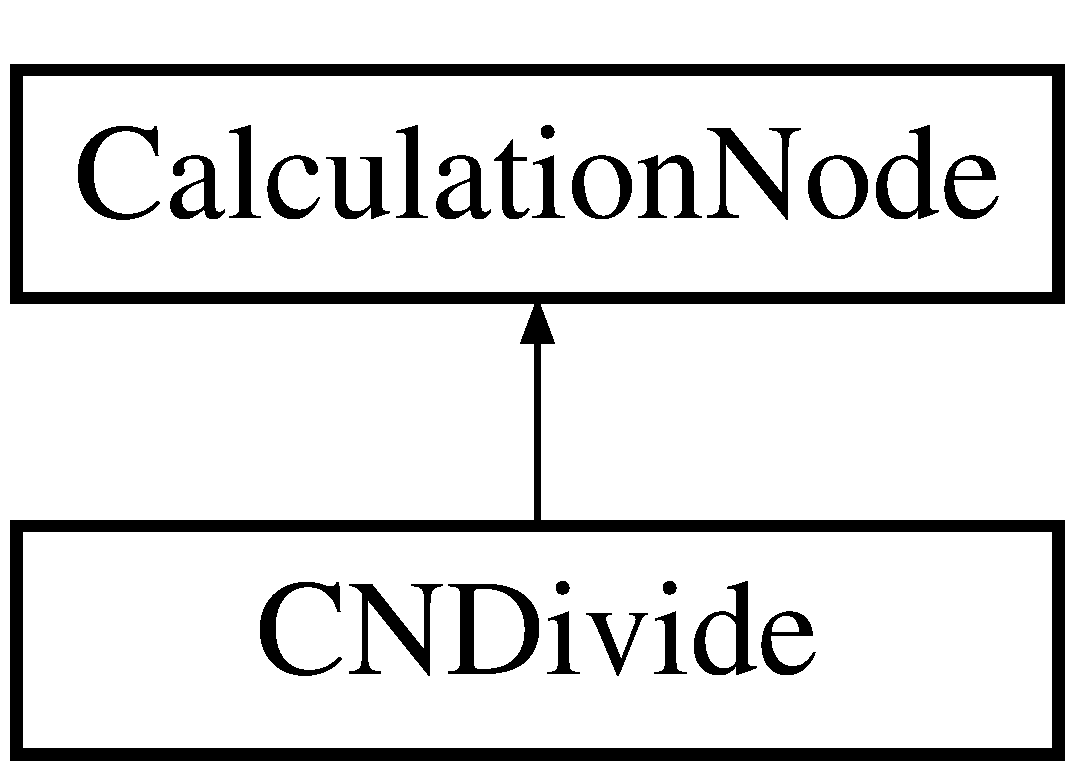
\includegraphics[height=2.000000cm]{classCNDivide}
\end{center}
\end{figure}
\subsection*{Public Member Functions}
\begin{DoxyCompactItemize}
\item 
{\bfseries C\+N\+Divide} (\hyperlink{classCalculationNode}{Calculation\+Node} $\ast$\+\_\+left, \hyperlink{classCalculationNode}{Calculation\+Node} $\ast$\+\_\+right)\hypertarget{classCNDivide_afeb9424f787f42ebf0edb7926a0e80fd}{}\label{classCNDivide_afeb9424f787f42ebf0edb7926a0e80fd}

\item 
virtual double {\bfseries evaluate} () const \hypertarget{classCNDivide_a416c36cec11a481a20bbe3409c1e42db}{}\label{classCNDivide_a416c36cec11a481a20bbe3409c1e42db}

\item 
virtual double {\bfseries evaluate\+At\+State} (std\+::map$<$ int, double $>$ starting\+State) const \hypertarget{classCNDivide_a77752426072bc2bda3b0ca4fdc03f871}{}\label{classCNDivide_a77752426072bc2bda3b0ca4fdc03f871}

\item 
virtual bool {\bfseries test\+Node\+Ids} () const \hypertarget{classCNDivide_a411f954df8b87778f20058ce6601d3f8}{}\label{classCNDivide_a411f954df8b87778f20058ce6601d3f8}

\item 
virtual std\+::string {\bfseries to\+String} () const \hypertarget{classCNDivide_a301fb85c372986362aa6b4930f0d79c5}{}\label{classCNDivide_a301fb85c372986362aa6b4930f0d79c5}

\end{DoxyCompactItemize}
\subsection*{Additional Inherited Members}


The documentation for this class was generated from the following file\+:\begin{DoxyCompactItemize}
\item 
/home/mate/\+Documents/\+Programming/\+Research/\+Multilayer\+Network\+Model/\+Multilayer\+Network\+Model/sources/core/\+Dynamical\+Equation/include/Calculation\+Node.\+hh\end{DoxyCompactItemize}

\hypertarget{classCNId}{}\section{C\+N\+Id Class Reference}
\label{classCNId}\index{C\+N\+Id@{C\+N\+Id}}
Inheritance diagram for C\+N\+Id\+:\begin{figure}[H]
\begin{center}
\leavevmode
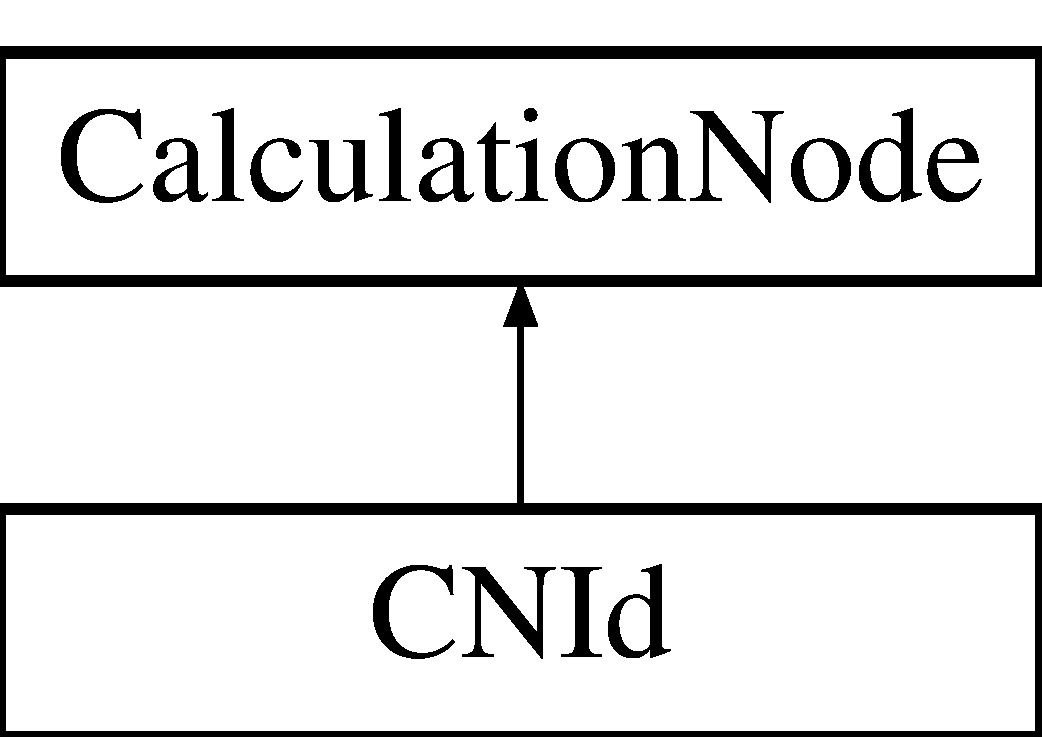
\includegraphics[height=2.000000cm]{classCNId}
\end{center}
\end{figure}
\subsection*{Public Member Functions}
\begin{DoxyCompactItemize}
\item 
{\bfseries C\+N\+Id} (int \+\_\+id)\hypertarget{classCNId_ad36125d5115c0c75783a23e1e4ad55b2}{}\label{classCNId_ad36125d5115c0c75783a23e1e4ad55b2}

\item 
int {\bfseries get\+Id} ()\hypertarget{classCNId_ae0c2d402de892ef8783e6f5281ece008}{}\label{classCNId_ae0c2d402de892ef8783e6f5281ece008}

\item 
void {\bfseries set\+Node} (\hyperlink{classNode}{Node} $\ast$node)\hypertarget{classCNId_a25b7d25adf35e61b0d1b0e67862354f4}{}\label{classCNId_a25b7d25adf35e61b0d1b0e67862354f4}

\item 
virtual double {\bfseries evaluate} () const \hypertarget{classCNId_a5f6b3bbc1a6daaef9a11cdc80aff920c}{}\label{classCNId_a5f6b3bbc1a6daaef9a11cdc80aff920c}

\item 
virtual double {\bfseries evaluate\+At\+State} (std\+::map$<$ int, double $>$ starting\+State) const \hypertarget{classCNId_aacf48e3e3766cc1d54a9af8532d747ec}{}\label{classCNId_aacf48e3e3766cc1d54a9af8532d747ec}

\item 
virtual bool {\bfseries test\+Node\+Ids} () const \hypertarget{classCNId_a0bc1a04e94dfbb047ad53dd6682bf071}{}\label{classCNId_a0bc1a04e94dfbb047ad53dd6682bf071}

\item 
virtual std\+::string {\bfseries to\+String} () const \hypertarget{classCNId_ae853b898d20c008bdddf799ed971f30a}{}\label{classCNId_ae853b898d20c008bdddf799ed971f30a}

\end{DoxyCompactItemize}
\subsection*{Additional Inherited Members}


The documentation for this class was generated from the following files\+:\begin{DoxyCompactItemize}
\item 
/home/mate/\+Documents/\+Programming/\+Research/\+Multilayer\+Network\+Model/\+Multilayer\+Network\+Model/sources/core/\+Dynamical\+Equation/include/Calculation\+Node.\+hh\item 
/home/mate/\+Documents/\+Programming/\+Research/\+Multilayer\+Network\+Model/\+Multilayer\+Network\+Model/sources/core/\+Dynamical\+Equation/src/Calculation\+Node.\+cc\end{DoxyCompactItemize}

\hypertarget{classCNMultiply}{}\section{C\+N\+Multiply Class Reference}
\label{classCNMultiply}\index{C\+N\+Multiply@{C\+N\+Multiply}}
Inheritance diagram for C\+N\+Multiply\+:\begin{figure}[H]
\begin{center}
\leavevmode
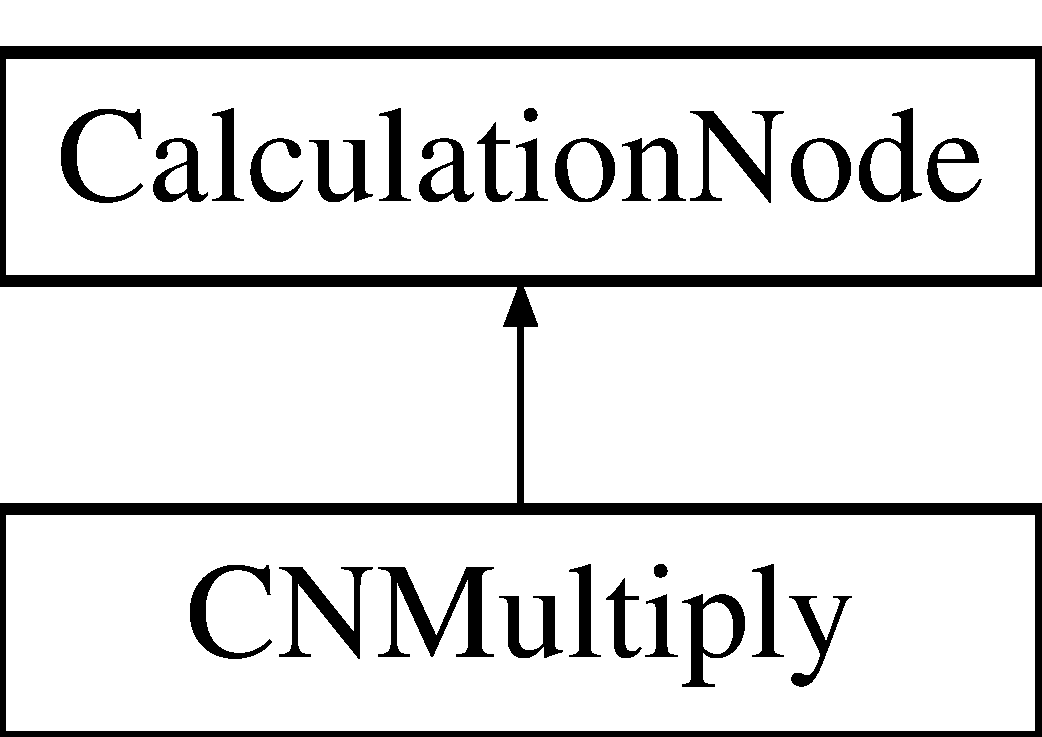
\includegraphics[height=2.000000cm]{classCNMultiply}
\end{center}
\end{figure}
\subsection*{Public Member Functions}
\begin{DoxyCompactItemize}
\item 
{\bfseries C\+N\+Multiply} (\hyperlink{classCalculationNode}{Calculation\+Node} $\ast$\+\_\+left, \hyperlink{classCalculationNode}{Calculation\+Node} $\ast$\+\_\+right)\hypertarget{classCNMultiply_a440c0e25b1fb642c95757a9118634874}{}\label{classCNMultiply_a440c0e25b1fb642c95757a9118634874}

\item 
virtual double {\bfseries evaluate} () const \hypertarget{classCNMultiply_a51ce205165bfa5842002721332c14f5c}{}\label{classCNMultiply_a51ce205165bfa5842002721332c14f5c}

\item 
virtual double {\bfseries evaluate\+At\+State} (std\+::map$<$ int, double $>$ starting\+State) const \hypertarget{classCNMultiply_a8daa0d3ea8f08db43b6e168f6ca9527b}{}\label{classCNMultiply_a8daa0d3ea8f08db43b6e168f6ca9527b}

\item 
virtual bool {\bfseries test\+Node\+Ids} () const \hypertarget{classCNMultiply_a9ffc252a3cc6ccdb3ef9ee4700f0ac18}{}\label{classCNMultiply_a9ffc252a3cc6ccdb3ef9ee4700f0ac18}

\item 
virtual std\+::string {\bfseries to\+String} () const \hypertarget{classCNMultiply_a55edebadef3ea3df839dd8779f1e2e13}{}\label{classCNMultiply_a55edebadef3ea3df839dd8779f1e2e13}

\end{DoxyCompactItemize}
\subsection*{Additional Inherited Members}


The documentation for this class was generated from the following file\+:\begin{DoxyCompactItemize}
\item 
/home/mate/\+Documents/\+Programming/\+Research/\+Multilayer\+Network\+Model/\+Multilayer\+Network\+Model/sources/core/\+Dynamical\+Equation/include/Calculation\+Node.\+hh\end{DoxyCompactItemize}

\hypertarget{classCNNegate}{}\section{C\+N\+Negate Class Reference}
\label{classCNNegate}\index{C\+N\+Negate@{C\+N\+Negate}}
Inheritance diagram for C\+N\+Negate\+:\begin{figure}[H]
\begin{center}
\leavevmode
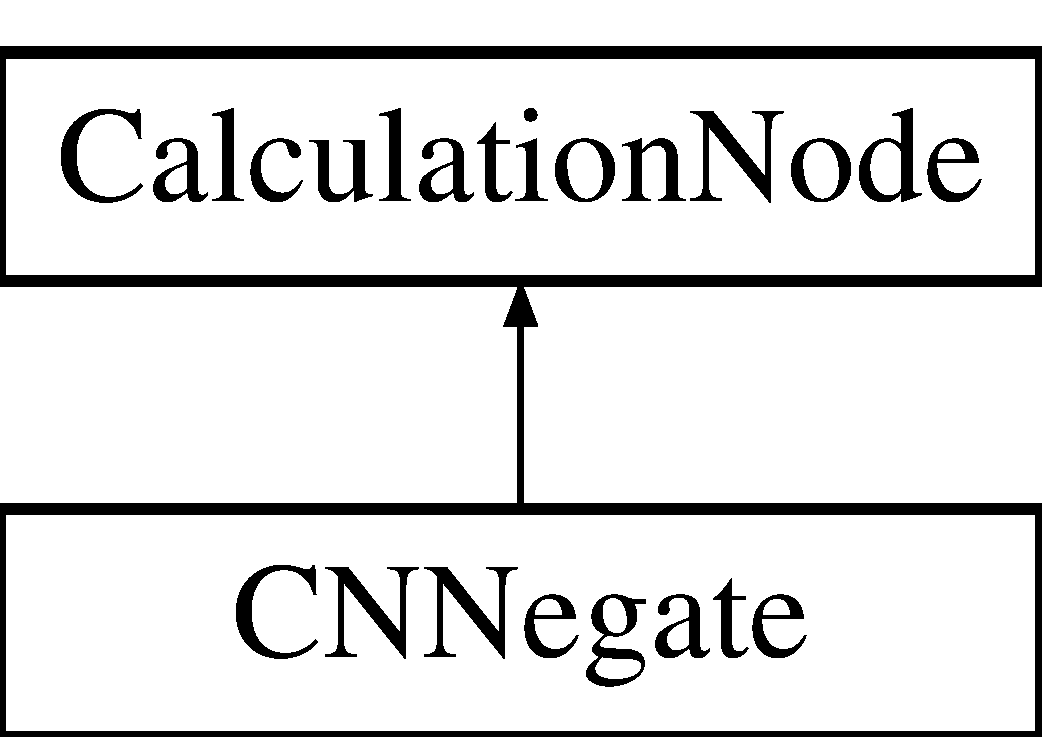
\includegraphics[height=2.000000cm]{classCNNegate}
\end{center}
\end{figure}
\subsection*{Public Member Functions}
\begin{DoxyCompactItemize}
\item 
{\bfseries C\+N\+Negate} (\hyperlink{classCalculationNode}{Calculation\+Node} $\ast$\+\_\+right)\hypertarget{classCNNegate_a7ed8699cfcdf9e6cb4e08c2f386ec8aa}{}\label{classCNNegate_a7ed8699cfcdf9e6cb4e08c2f386ec8aa}

\item 
virtual double {\bfseries evaluate} () const \hypertarget{classCNNegate_ad8742ef807da75fea0d512467d5331cd}{}\label{classCNNegate_ad8742ef807da75fea0d512467d5331cd}

\item 
virtual double {\bfseries evaluate\+At\+State} (std\+::map$<$ int, double $>$ starting\+State) const \hypertarget{classCNNegate_a466eaeee589ea62f77dab230b4da9ab7}{}\label{classCNNegate_a466eaeee589ea62f77dab230b4da9ab7}

\item 
virtual bool {\bfseries test\+Node\+Ids} () const \hypertarget{classCNNegate_ad03475bf5217a1673057e74f60b7b7fe}{}\label{classCNNegate_ad03475bf5217a1673057e74f60b7b7fe}

\item 
virtual std\+::string {\bfseries to\+String} () const \hypertarget{classCNNegate_a8cf6b243b14cfbeb28434f301303d1a9}{}\label{classCNNegate_a8cf6b243b14cfbeb28434f301303d1a9}

\end{DoxyCompactItemize}
\subsection*{Additional Inherited Members}


The documentation for this class was generated from the following file\+:\begin{DoxyCompactItemize}
\item 
/home/mate/\+Documents/\+Programming/\+Research/\+Multilayer\+Network\+Model/\+Multilayer\+Network\+Model/sources/core/\+Dynamical\+Equation/include/Calculation\+Node.\+hh\end{DoxyCompactItemize}

\hypertarget{classCNPower}{}\section{C\+N\+Power Class Reference}
\label{classCNPower}\index{C\+N\+Power@{C\+N\+Power}}
Inheritance diagram for C\+N\+Power\+:\begin{figure}[H]
\begin{center}
\leavevmode
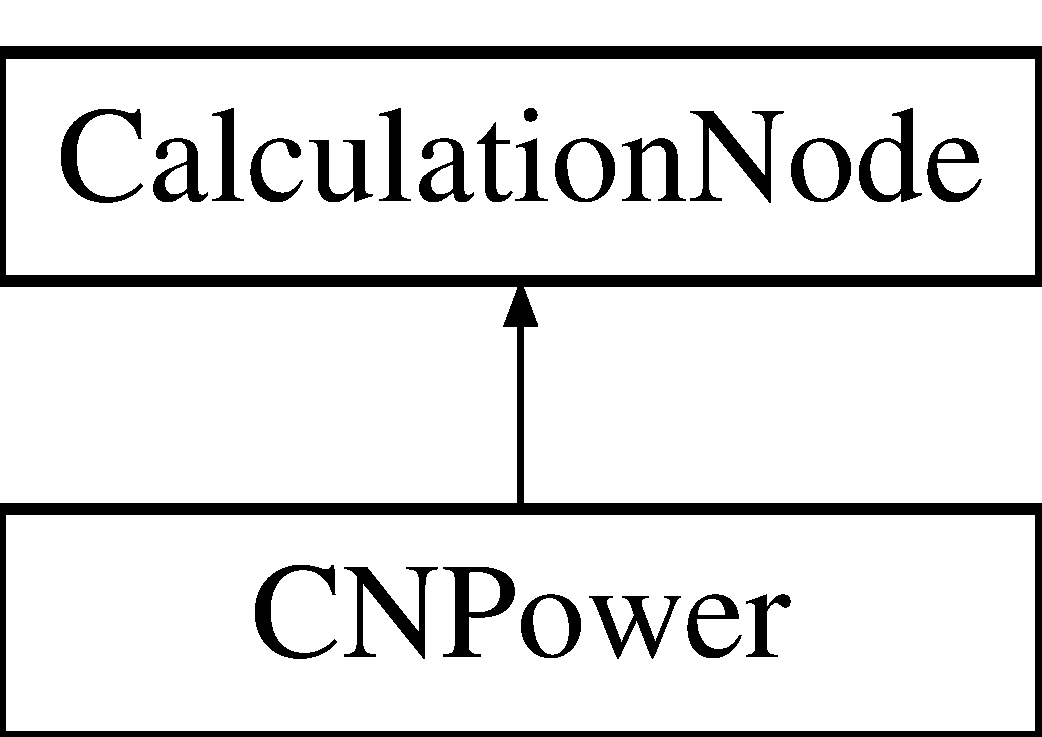
\includegraphics[height=2.000000cm]{classCNPower}
\end{center}
\end{figure}
\subsection*{Public Member Functions}
\begin{DoxyCompactItemize}
\item 
{\bfseries C\+N\+Power} (\hyperlink{classCalculationNode}{Calculation\+Node} $\ast$\+\_\+left, \hyperlink{classCalculationNode}{Calculation\+Node} $\ast$\+\_\+right)\hypertarget{classCNPower_ac5ba8a91170451bc06afbf7153d7f707}{}\label{classCNPower_ac5ba8a91170451bc06afbf7153d7f707}

\item 
virtual double {\bfseries evaluate} () const \hypertarget{classCNPower_a9461646cf8e9fc0cb54318e04d73ed72}{}\label{classCNPower_a9461646cf8e9fc0cb54318e04d73ed72}

\item 
virtual double {\bfseries evaluate\+At\+State} (std\+::map$<$ int, double $>$ starting\+State) const \hypertarget{classCNPower_af4a31cbe51bc44fba203bda91d46384f}{}\label{classCNPower_af4a31cbe51bc44fba203bda91d46384f}

\item 
virtual bool {\bfseries test\+Node\+Ids} () const \hypertarget{classCNPower_a3d1e004e5e71954037b2ea46f54cd438}{}\label{classCNPower_a3d1e004e5e71954037b2ea46f54cd438}

\item 
virtual std\+::string {\bfseries to\+String} () const \hypertarget{classCNPower_a5d9c427cba2ea13f2bf91ecadcac50ef}{}\label{classCNPower_a5d9c427cba2ea13f2bf91ecadcac50ef}

\end{DoxyCompactItemize}
\subsection*{Additional Inherited Members}


The documentation for this class was generated from the following file\+:\begin{DoxyCompactItemize}
\item 
/home/mate/\+Documents/\+Programming/\+Research/\+Multilayer\+Network\+Model/\+Multilayer\+Network\+Model/src/core/include/Calculation\+Node.\+hh\end{DoxyCompactItemize}

\hypertarget{classCNSubtract}{}\section{C\+N\+Subtract Class Reference}
\label{classCNSubtract}\index{C\+N\+Subtract@{C\+N\+Subtract}}
Inheritance diagram for C\+N\+Subtract\+:\begin{figure}[H]
\begin{center}
\leavevmode
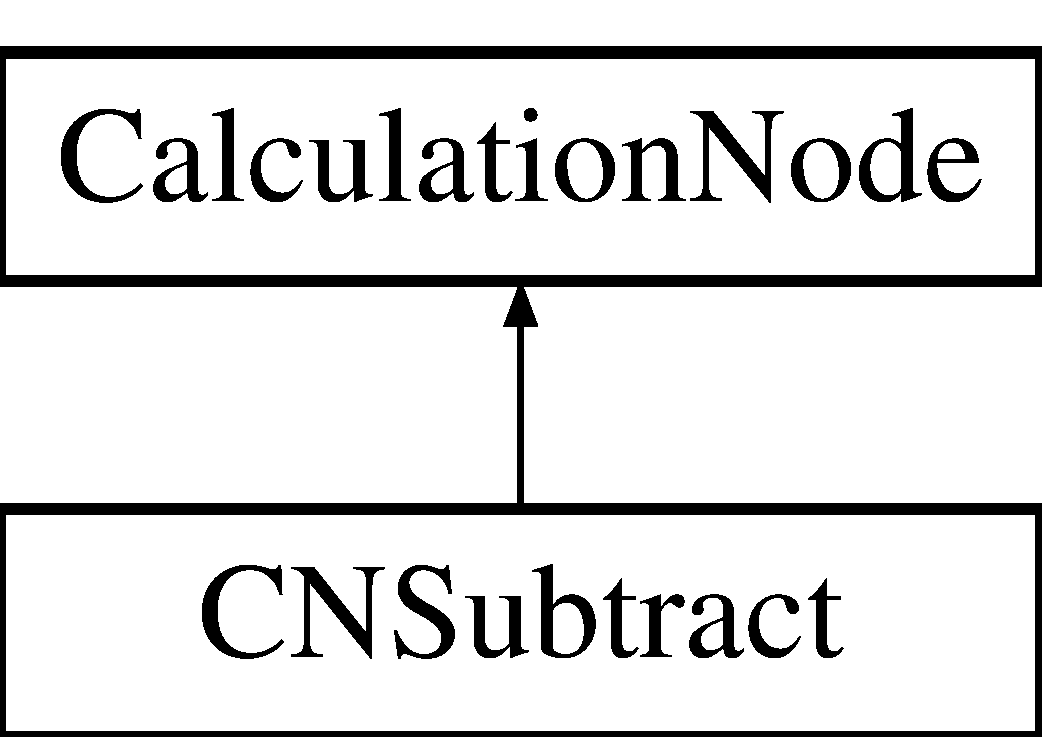
\includegraphics[height=2.000000cm]{classCNSubtract}
\end{center}
\end{figure}
\subsection*{Public Member Functions}
\begin{DoxyCompactItemize}
\item 
{\bfseries C\+N\+Subtract} (\hyperlink{classCalculationNode}{Calculation\+Node} $\ast$\+\_\+left, \hyperlink{classCalculationNode}{Calculation\+Node} $\ast$\+\_\+right)\hypertarget{classCNSubtract_ab72c2b6679137655582d2001ac420dbf}{}\label{classCNSubtract_ab72c2b6679137655582d2001ac420dbf}

\item 
virtual double {\bfseries evaluate} () const \hypertarget{classCNSubtract_ae57879411a77bf2a5b16f28aa488a3d6}{}\label{classCNSubtract_ae57879411a77bf2a5b16f28aa488a3d6}

\item 
virtual double {\bfseries evaluate\+At\+State} (std\+::map$<$ int, double $>$ starting\+State) const \hypertarget{classCNSubtract_aa1d22fea2c4d0cdd26e64725d2be5205}{}\label{classCNSubtract_aa1d22fea2c4d0cdd26e64725d2be5205}

\item 
virtual bool \hyperlink{classCNSubtract_a83d03d12f8b0b209c78dda0d783453e1}{test\+Node\+Ids} () const 
\item 
virtual std\+::string {\bfseries to\+String} () const \hypertarget{classCNSubtract_a19ed00fcb52d52d40d97ed79a62e6dcd}{}\label{classCNSubtract_a19ed00fcb52d52d40d97ed79a62e6dcd}

\end{DoxyCompactItemize}
\subsection*{Additional Inherited Members}


\subsection{Member Function Documentation}
\index{C\+N\+Subtract@{C\+N\+Subtract}!test\+Node\+Ids@{test\+Node\+Ids}}
\index{test\+Node\+Ids@{test\+Node\+Ids}!C\+N\+Subtract@{C\+N\+Subtract}}
\subsubsection[{\texorpdfstring{test\+Node\+Ids() const }{testNodeIds() const }}]{\setlength{\rightskip}{0pt plus 5cm}virtual bool C\+N\+Subtract\+::test\+Node\+Ids (
\begin{DoxyParamCaption}
{}
\end{DoxyParamCaption}
) const\hspace{0.3cm}{\ttfamily [inline]}, {\ttfamily [virtual]}}\hypertarget{classCNSubtract_a83d03d12f8b0b209c78dda0d783453e1}{}\label{classCNSubtract_a83d03d12f8b0b209c78dda0d783453e1}
Used only for testing puposes. Compared the ID type \hyperlink{classCalculationNode}{Calculation\+Node}\textquotesingle{}s id field to the assigned node\textquotesingle{}s id. 

Implements \hyperlink{classCalculationNode_a4089a2510d7c345a9632843a3fed4f0e}{Calculation\+Node}.



The documentation for this class was generated from the following file\+:\begin{DoxyCompactItemize}
\item 
/home/mate/\+Documents/\+Programming/\+Research/\+Multilayer\+Network\+Model/\+Multilayer\+Network\+Model/sources/core/\+Dynamical\+Equation/include/Calculation\+Node.\+hh\end{DoxyCompactItemize}

\hypertarget{classCrtAllocator}{}\section{Crt\+Allocator Class Reference}
\label{classCrtAllocator}\index{Crt\+Allocator@{Crt\+Allocator}}


C-\/runtime library allocator.  




{\ttfamily \#include $<$allocators.\+h$>$}

\subsection*{Public Member Functions}
\begin{DoxyCompactItemize}
\item 
void $\ast$ {\bfseries Malloc} (size\+\_\+t size)\hypertarget{classCrtAllocator_acd720631f8c094041afa6c7951f0d935}{}\label{classCrtAllocator_acd720631f8c094041afa6c7951f0d935}

\item 
void $\ast$ {\bfseries Realloc} (void $\ast$original\+Ptr, size\+\_\+t original\+Size, size\+\_\+t new\+Size)\hypertarget{classCrtAllocator_a646bb6f68afe773a62a22f7f14f83e97}{}\label{classCrtAllocator_a646bb6f68afe773a62a22f7f14f83e97}

\end{DoxyCompactItemize}
\subsection*{Static Public Member Functions}
\begin{DoxyCompactItemize}
\item 
static void {\bfseries Free} (void $\ast$ptr)\hypertarget{classCrtAllocator_a5043907058d906dcb1291e9491560373}{}\label{classCrtAllocator_a5043907058d906dcb1291e9491560373}

\end{DoxyCompactItemize}
\subsection*{Static Public Attributes}
\begin{DoxyCompactItemize}
\item 
static const bool {\bfseries k\+Need\+Free} = true\hypertarget{classCrtAllocator_ac7df8398c529290f0cd5950d9492f524}{}\label{classCrtAllocator_ac7df8398c529290f0cd5950d9492f524}

\end{DoxyCompactItemize}


\subsection{Detailed Description}
C-\/runtime library allocator. 

This class is just wrapper for standard C library memory routines. \begin{DoxyNote}{Note}
implements Allocator concept 
\end{DoxyNote}


The documentation for this class was generated from the following file\+:\begin{DoxyCompactItemize}
\item 
/home/mate/\+Documents/\+Programming/\+Research/\+Multilayer\+Network\+Model/\+Multilayer\+Network\+Model/sources/external/rapidjson/allocators.\+h\end{DoxyCompactItemize}

\hypertarget{classCursorStreamWrapper}{}\section{Cursor\+Stream\+Wrapper$<$ Input\+Stream, Encoding $>$ Class Template Reference}
\label{classCursorStreamWrapper}\index{Cursor\+Stream\+Wrapper$<$ Input\+Stream, Encoding $>$@{Cursor\+Stream\+Wrapper$<$ Input\+Stream, Encoding $>$}}


Cursor stream wrapper for counting line and column number if error exists.  




{\ttfamily \#include $<$cursorstreamwrapper.\+h$>$}

Inheritance diagram for Cursor\+Stream\+Wrapper$<$ Input\+Stream, Encoding $>$\+:\begin{figure}[H]
\begin{center}
\leavevmode
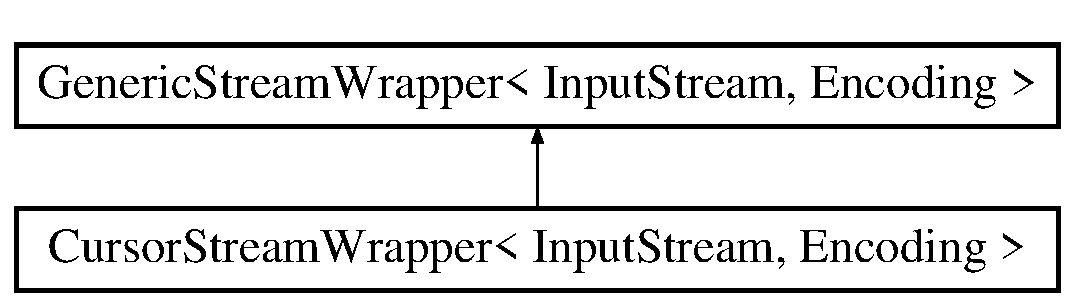
\includegraphics[height=2.000000cm]{classCursorStreamWrapper}
\end{center}
\end{figure}
\subsection*{Public Types}
\begin{DoxyCompactItemize}
\item 
typedef Encoding\+::\+Ch {\bfseries Ch}\hypertarget{classCursorStreamWrapper_a4bab1186bfeebbcf00719c2613b0dca6}{}\label{classCursorStreamWrapper_a4bab1186bfeebbcf00719c2613b0dca6}

\end{DoxyCompactItemize}
\subsection*{Public Member Functions}
\begin{DoxyCompactItemize}
\item 
{\bfseries Cursor\+Stream\+Wrapper} (Input\+Stream \&is)\hypertarget{classCursorStreamWrapper_a8d9a0109e19ab4fb7a79091cefe608a7}{}\label{classCursorStreamWrapper_a8d9a0109e19ab4fb7a79091cefe608a7}

\item 
Ch {\bfseries Take} ()\hypertarget{classCursorStreamWrapper_af0bbad24ff7ad101cdf9842760deb0f6}{}\label{classCursorStreamWrapper_af0bbad24ff7ad101cdf9842760deb0f6}

\item 
size\+\_\+t \hyperlink{classCursorStreamWrapper_ae78cc02ed7308771a57ee2b858925b36}{Get\+Line} () const \hypertarget{classCursorStreamWrapper_ae78cc02ed7308771a57ee2b858925b36}{}\label{classCursorStreamWrapper_ae78cc02ed7308771a57ee2b858925b36}

\begin{DoxyCompactList}\small\item\em Get the error line number, if error exists. \end{DoxyCompactList}\item 
size\+\_\+t \hyperlink{classCursorStreamWrapper_a8e2764dc2434acb4bba99cf233206247}{Get\+Column} () const \hypertarget{classCursorStreamWrapper_a8e2764dc2434acb4bba99cf233206247}{}\label{classCursorStreamWrapper_a8e2764dc2434acb4bba99cf233206247}

\begin{DoxyCompactList}\small\item\em Get the error column number, if error exists. \end{DoxyCompactList}\end{DoxyCompactItemize}
\subsection*{Additional Inherited Members}


\subsection{Detailed Description}
\subsubsection*{template$<$typename Input\+Stream, typename Encoding = U\+T\+F8$<$$>$$>$\\*
class Cursor\+Stream\+Wrapper$<$ Input\+Stream, Encoding $>$}

Cursor stream wrapper for counting line and column number if error exists. 


\begin{DoxyTemplParams}{Template Parameters}
{\em Input\+Stream} & Any stream that implements Stream Concept \\
\hline
\end{DoxyTemplParams}


The documentation for this class was generated from the following file\+:\begin{DoxyCompactItemize}
\item 
/home/mate/\+Documents/\+Programming/\+Research/\+Multilayer\+Network\+Model/\+Multilayer\+Network\+Model/sources/external/rapidjson/cursorstreamwrapper.\+h\end{DoxyCompactItemize}

\hypertarget{unionGenericValue_1_1Data}{}\section{Generic\+Value$<$ Encoding, Allocator $>$\+:\+:Data Union Reference}
\label{unionGenericValue_1_1Data}\index{Generic\+Value$<$ Encoding, Allocator $>$\+::\+Data@{Generic\+Value$<$ Encoding, Allocator $>$\+::\+Data}}
\subsection*{Public Attributes}
\begin{DoxyCompactItemize}
\item 
\hyperlink{structGenericValue_1_1String}{String} {\bfseries s}\hypertarget{unionGenericValue_1_1Data_a6872a4b93763944063b425e6c001ed2b}{}\label{unionGenericValue_1_1Data_a6872a4b93763944063b425e6c001ed2b}

\item 
\hyperlink{structGenericValue_1_1ShortString}{Short\+String} {\bfseries ss}\hypertarget{unionGenericValue_1_1Data_a410e39a5dc296eb3b152b54193740e4c}{}\label{unionGenericValue_1_1Data_a410e39a5dc296eb3b152b54193740e4c}

\item 
\hyperlink{unionGenericValue_1_1Number}{Number} {\bfseries n}\hypertarget{unionGenericValue_1_1Data_a243007cce2f4b75bea3e3c1ee4c3c239}{}\label{unionGenericValue_1_1Data_a243007cce2f4b75bea3e3c1ee4c3c239}

\item 
\hyperlink{structGenericValue_1_1ObjectData}{Object\+Data} {\bfseries o}\hypertarget{unionGenericValue_1_1Data_af6417eca530fba0d8bd65d309628eb11}{}\label{unionGenericValue_1_1Data_af6417eca530fba0d8bd65d309628eb11}

\item 
\hyperlink{structGenericValue_1_1ArrayData}{Array\+Data} {\bfseries a}\hypertarget{unionGenericValue_1_1Data_aeac31cf55bf5a024cead5ecb63e4fd48}{}\label{unionGenericValue_1_1Data_aeac31cf55bf5a024cead5ecb63e4fd48}

\item 
\hyperlink{structGenericValue_1_1Flag}{Flag} {\bfseries f}\hypertarget{unionGenericValue_1_1Data_ad8572112da083c775ce21bcbca96b2ab}{}\label{unionGenericValue_1_1Data_ad8572112da083c775ce21bcbca96b2ab}

\end{DoxyCompactItemize}


The documentation for this union was generated from the following file\+:\begin{DoxyCompactItemize}
\item 
/home/mate/\+Documents/\+Programming/\+Research/\+Multilayer\+Network\+Model/\+Multilayer\+Network\+Model/src/external/rapidjson/\hyperlink{document_8h}{document.\+h}\end{DoxyCompactItemize}

\hypertarget{classinternal_1_1DecodedStream}{}\section{internal\+:\+:Decoded\+Stream$<$ Source\+Stream, Encoding $>$ Class Template Reference}
\label{classinternal_1_1DecodedStream}\index{internal\+::\+Decoded\+Stream$<$ Source\+Stream, Encoding $>$@{internal\+::\+Decoded\+Stream$<$ Source\+Stream, Encoding $>$}}
\subsection*{Public Member Functions}
\begin{DoxyCompactItemize}
\item 
{\bfseries Decoded\+Stream} (Source\+Stream \&ss)\hypertarget{classinternal_1_1DecodedStream_a45cf40c4e515be8aaa8cd020eaa67595}{}\label{classinternal_1_1DecodedStream_a45cf40c4e515be8aaa8cd020eaa67595}

\item 
unsigned {\bfseries Peek} ()\hypertarget{classinternal_1_1DecodedStream_ac78f2cbc03ae0d79a0fcfe6d56589d70}{}\label{classinternal_1_1DecodedStream_ac78f2cbc03ae0d79a0fcfe6d56589d70}

\item 
unsigned {\bfseries Take} ()\hypertarget{classinternal_1_1DecodedStream_a62b45969ce169bef1da0600490329857}{}\label{classinternal_1_1DecodedStream_a62b45969ce169bef1da0600490329857}

\end{DoxyCompactItemize}


The documentation for this class was generated from the following file\+:\begin{DoxyCompactItemize}
\item 
/home/mate/\+Documents/\+Programming/\+Research/\+Multilayer\+Network\+Model/\+Multilayer\+Network\+Model/sources/external/rapidjson/internal/regex.\+h\end{DoxyCompactItemize}

\hypertarget{structinternal_1_1DiyFp}{}\section{internal\+:\+:Diy\+Fp Struct Reference}
\label{structinternal_1_1DiyFp}\index{internal\+::\+Diy\+Fp@{internal\+::\+Diy\+Fp}}
\subsection*{Public Member Functions}
\begin{DoxyCompactItemize}
\item 
{\bfseries Diy\+Fp} (uint64\+\_\+t fp, int exp)\hypertarget{structinternal_1_1DiyFp_a9a8f2f5c49dfa0dee4a527f0829cc2e5}{}\label{structinternal_1_1DiyFp_a9a8f2f5c49dfa0dee4a527f0829cc2e5}

\item 
{\bfseries Diy\+Fp} (double d)\hypertarget{structinternal_1_1DiyFp_adc132c7da4c8e3ee5ae12efdcf6dbf7c}{}\label{structinternal_1_1DiyFp_adc132c7da4c8e3ee5ae12efdcf6dbf7c}

\item 
\hyperlink{structinternal_1_1DiyFp}{Diy\+Fp} {\bfseries operator-\/} (const \hyperlink{structinternal_1_1DiyFp}{Diy\+Fp} \&rhs) const \hypertarget{structinternal_1_1DiyFp_ade3efb95107203f2327fc3d5a802d4b7}{}\label{structinternal_1_1DiyFp_ade3efb95107203f2327fc3d5a802d4b7}

\item 
\hyperlink{structinternal_1_1DiyFp}{Diy\+Fp} \hyperlink{structinternal_1_1DiyFp_ab536022d225b3014c98517a2dec4b986}{operator$\ast$} (const \hyperlink{structinternal_1_1DiyFp}{Diy\+Fp} \&rhs) const 
\item 
\hyperlink{structinternal_1_1DiyFp}{Diy\+Fp} {\bfseries Normalize} () const \hypertarget{structinternal_1_1DiyFp_adae1948b1bb65d950cd3801a4a2bb7fd}{}\label{structinternal_1_1DiyFp_adae1948b1bb65d950cd3801a4a2bb7fd}

\item 
\hyperlink{structinternal_1_1DiyFp}{Diy\+Fp} {\bfseries Normalize\+Boundary} () const \hypertarget{structinternal_1_1DiyFp_a1a4589d19230c9930d7f3dd5a9b7f7e7}{}\label{structinternal_1_1DiyFp_a1a4589d19230c9930d7f3dd5a9b7f7e7}

\item 
void {\bfseries Normalized\+Boundaries} (\hyperlink{structinternal_1_1DiyFp}{Diy\+Fp} $\ast$minus, \hyperlink{structinternal_1_1DiyFp}{Diy\+Fp} $\ast$plus) const \hypertarget{structinternal_1_1DiyFp_a64e623c1742d1d5ad551ab456f0deb62}{}\label{structinternal_1_1DiyFp_a64e623c1742d1d5ad551ab456f0deb62}

\item 
double {\bfseries To\+Double} () const \hypertarget{structinternal_1_1DiyFp_a9bbdcfcf5d1b3a7b16a8f5f860d74038}{}\label{structinternal_1_1DiyFp_a9bbdcfcf5d1b3a7b16a8f5f860d74038}

\end{DoxyCompactItemize}
\subsection*{Public Attributes}
\begin{DoxyCompactItemize}
\item 
uint64\+\_\+t {\bfseries f}\hypertarget{structinternal_1_1DiyFp_a09b9217a86e8a2e6aa8d2d48fc351008}{}\label{structinternal_1_1DiyFp_a09b9217a86e8a2e6aa8d2d48fc351008}

\item 
int {\bfseries e}\hypertarget{structinternal_1_1DiyFp_afa9db335eeb61c7f966d888d89b1e6f2}{}\label{structinternal_1_1DiyFp_afa9db335eeb61c7f966d888d89b1e6f2}

\end{DoxyCompactItemize}
\subsection*{Static Public Attributes}
\begin{DoxyCompactItemize}
\item 
static const int {\bfseries k\+Diy\+Significand\+Size} = 64\hypertarget{structinternal_1_1DiyFp_aac30e0c32d43425ac403281fc9b0cee4}{}\label{structinternal_1_1DiyFp_aac30e0c32d43425ac403281fc9b0cee4}

\item 
static const int {\bfseries k\+Dp\+Significand\+Size} = 52\hypertarget{structinternal_1_1DiyFp_a037aed0fa0b66af0a13657418edef19e}{}\label{structinternal_1_1DiyFp_a037aed0fa0b66af0a13657418edef19e}

\item 
static const int {\bfseries k\+Dp\+Exponent\+Bias} = 0x3\+F\+F + k\+Dp\+Significand\+Size\hypertarget{structinternal_1_1DiyFp_a38b6f864ae0859d43fa96c3ff27959be}{}\label{structinternal_1_1DiyFp_a38b6f864ae0859d43fa96c3ff27959be}

\item 
static const int {\bfseries k\+Dp\+Max\+Exponent} = 0x7\+F\+F -\/ k\+Dp\+Exponent\+Bias\hypertarget{structinternal_1_1DiyFp_a80535a5594dae96fc482757a54162c7d}{}\label{structinternal_1_1DiyFp_a80535a5594dae96fc482757a54162c7d}

\item 
static const int {\bfseries k\+Dp\+Min\+Exponent} = -\/k\+Dp\+Exponent\+Bias\hypertarget{structinternal_1_1DiyFp_a9ad1b0cdbab318e45d2bc48e64707ef3}{}\label{structinternal_1_1DiyFp_a9ad1b0cdbab318e45d2bc48e64707ef3}

\item 
static const int {\bfseries k\+Dp\+Denormal\+Exponent} = -\/k\+Dp\+Exponent\+Bias + 1\hypertarget{structinternal_1_1DiyFp_a994f16a1247a290cfc3a875715e3a92b}{}\label{structinternal_1_1DiyFp_a994f16a1247a290cfc3a875715e3a92b}

\item 
static const uint64\+\_\+t {\bfseries k\+Dp\+Exponent\+Mask} = \hyperlink{rapidjson_8h_aaee1245f375a71be1ac9b8a07ba5fb8f}{R\+A\+P\+I\+D\+J\+S\+O\+N\+\_\+\+U\+I\+N\+T64\+\_\+\+C2}(0x7\+F\+F00000, 0x00000000)\hypertarget{structinternal_1_1DiyFp_aaacbf068c44275f4451db750938bd1d3}{}\label{structinternal_1_1DiyFp_aaacbf068c44275f4451db750938bd1d3}

\item 
static const uint64\+\_\+t {\bfseries k\+Dp\+Significand\+Mask} = \hyperlink{rapidjson_8h_aaee1245f375a71be1ac9b8a07ba5fb8f}{R\+A\+P\+I\+D\+J\+S\+O\+N\+\_\+\+U\+I\+N\+T64\+\_\+\+C2}(0x000\+F\+F\+F\+F\+F, 0x\+F\+F\+F\+F\+F\+F\+F\+F)\hypertarget{structinternal_1_1DiyFp_a841ef0ae29ccd2889e7f96aad76b0179}{}\label{structinternal_1_1DiyFp_a841ef0ae29ccd2889e7f96aad76b0179}

\item 
static const uint64\+\_\+t {\bfseries k\+Dp\+Hidden\+Bit} = \hyperlink{rapidjson_8h_aaee1245f375a71be1ac9b8a07ba5fb8f}{R\+A\+P\+I\+D\+J\+S\+O\+N\+\_\+\+U\+I\+N\+T64\+\_\+\+C2}(0x00100000, 0x00000000)\hypertarget{structinternal_1_1DiyFp_a43ea451ce20095b1ff53cccf132ca15f}{}\label{structinternal_1_1DiyFp_a43ea451ce20095b1ff53cccf132ca15f}

\end{DoxyCompactItemize}


\subsection{Member Function Documentation}
\index{internal\+::\+Diy\+Fp@{internal\+::\+Diy\+Fp}!operator$\ast$@{operator$\ast$}}
\index{operator$\ast$@{operator$\ast$}!internal\+::\+Diy\+Fp@{internal\+::\+Diy\+Fp}}
\subsubsection[{\texorpdfstring{operator$\ast$(const Diy\+Fp \&rhs) const }{operator*(const DiyFp &rhs) const }}]{\setlength{\rightskip}{0pt plus 5cm}{\bf Diy\+Fp} internal\+::\+Diy\+Fp\+::operator$\ast$ (
\begin{DoxyParamCaption}
\item[{const {\bf Diy\+Fp} \&}]{rhs}
\end{DoxyParamCaption}
) const\hspace{0.3cm}{\ttfamily [inline]}}\hypertarget{structinternal_1_1DiyFp_ab536022d225b3014c98517a2dec4b986}{}\label{structinternal_1_1DiyFp_ab536022d225b3014c98517a2dec4b986}
mult\+\_\+round 

The documentation for this struct was generated from the following file\+:\begin{DoxyCompactItemize}
\item 
/home/mate/\+Documents/\+Programming/\+Research/\+Multilayer\+Network\+Model/\+Multilayer\+Network\+Model/src/external/rapidjson/internal/diyfp.\+h\end{DoxyCompactItemize}

\hypertarget{classinternal_1_1Double}{}\section{internal\+:\+:Double Class Reference}
\label{classinternal_1_1Double}\index{internal\+::\+Double@{internal\+::\+Double}}
\subsection*{Public Member Functions}
\begin{DoxyCompactItemize}
\item 
{\bfseries Double} (double d)\hypertarget{classinternal_1_1Double_ad66f3b914570ce62e9f16083117f3e4f}{}\label{classinternal_1_1Double_ad66f3b914570ce62e9f16083117f3e4f}

\item 
{\bfseries Double} (uint64\+\_\+t u)\hypertarget{classinternal_1_1Double_a293a7ca841d847ea3e83ffa28b68601f}{}\label{classinternal_1_1Double_a293a7ca841d847ea3e83ffa28b68601f}

\item 
double {\bfseries Value} () const \hypertarget{classinternal_1_1Double_af35ab8a9e1ee41b1fd8a97d5899cfa1d}{}\label{classinternal_1_1Double_af35ab8a9e1ee41b1fd8a97d5899cfa1d}

\item 
uint64\+\_\+t {\bfseries Uint64\+Value} () const \hypertarget{classinternal_1_1Double_a9b9f08386be36634cc79f2e9427517f9}{}\label{classinternal_1_1Double_a9b9f08386be36634cc79f2e9427517f9}

\item 
double {\bfseries Next\+Positive\+Double} () const \hypertarget{classinternal_1_1Double_a3da449454b6b7e7108ed1b9a00625b68}{}\label{classinternal_1_1Double_a3da449454b6b7e7108ed1b9a00625b68}

\item 
bool {\bfseries Sign} () const \hypertarget{classinternal_1_1Double_ad3f4421a50d77c3af20638a12ec8f168}{}\label{classinternal_1_1Double_ad3f4421a50d77c3af20638a12ec8f168}

\item 
uint64\+\_\+t {\bfseries Significand} () const \hypertarget{classinternal_1_1Double_a8c3f5cf8152af8588d32530238c35aad}{}\label{classinternal_1_1Double_a8c3f5cf8152af8588d32530238c35aad}

\item 
int {\bfseries Exponent} () const \hypertarget{classinternal_1_1Double_a39aa84d5dc24cf22ca44578fab515f44}{}\label{classinternal_1_1Double_a39aa84d5dc24cf22ca44578fab515f44}

\item 
bool {\bfseries Is\+Nan} () const \hypertarget{classinternal_1_1Double_a5c1ad93b8c866afdd5c2b412ef7bea98}{}\label{classinternal_1_1Double_a5c1ad93b8c866afdd5c2b412ef7bea98}

\item 
bool {\bfseries Is\+Inf} () const \hypertarget{classinternal_1_1Double_a2efab47ffbfa75e0fca1129263b86545}{}\label{classinternal_1_1Double_a2efab47ffbfa75e0fca1129263b86545}

\item 
bool {\bfseries Is\+Nan\+Or\+Inf} () const \hypertarget{classinternal_1_1Double_a5b5cc0b8552246f9e274b00a010bd676}{}\label{classinternal_1_1Double_a5b5cc0b8552246f9e274b00a010bd676}

\item 
bool {\bfseries Is\+Normal} () const \hypertarget{classinternal_1_1Double_ac34b7871eeb80d2b6bac48f144c97b51}{}\label{classinternal_1_1Double_ac34b7871eeb80d2b6bac48f144c97b51}

\item 
bool {\bfseries Is\+Zero} () const \hypertarget{classinternal_1_1Double_a6eb58f2690af582efeb9b76ef35c4c60}{}\label{classinternal_1_1Double_a6eb58f2690af582efeb9b76ef35c4c60}

\item 
uint64\+\_\+t {\bfseries Integer\+Significand} () const \hypertarget{classinternal_1_1Double_a96c5e0f06551e83565b5097950d30e32}{}\label{classinternal_1_1Double_a96c5e0f06551e83565b5097950d30e32}

\item 
int {\bfseries Integer\+Exponent} () const \hypertarget{classinternal_1_1Double_a8e16ee31d521fb56f0b98be427a9d47e}{}\label{classinternal_1_1Double_a8e16ee31d521fb56f0b98be427a9d47e}

\item 
uint64\+\_\+t {\bfseries To\+Bias} () const \hypertarget{classinternal_1_1Double_af8b543dc813f761d274824f7cef00a43}{}\label{classinternal_1_1Double_af8b543dc813f761d274824f7cef00a43}

\end{DoxyCompactItemize}
\subsection*{Static Public Member Functions}
\begin{DoxyCompactItemize}
\item 
static int {\bfseries Effective\+Significand\+Size} (int order)\hypertarget{classinternal_1_1Double_aa710fa4f5e06b0ff4348a13475688f13}{}\label{classinternal_1_1Double_aa710fa4f5e06b0ff4348a13475688f13}

\end{DoxyCompactItemize}


The documentation for this class was generated from the following file\+:\begin{DoxyCompactItemize}
\item 
/home/mate/\+Documents/\+Programming/\+Research/\+Multilayer\+Network\+Model/\+Multilayer\+Network\+Model/sources/external/rapidjson/internal/ieee754.\+h\end{DoxyCompactItemize}

\hypertarget{classDownwardInfluenceImpl}{}\section{Downward\+Influence\+Impl Class Reference}
\label{classDownwardInfluenceImpl}\index{Downward\+Influence\+Impl@{Downward\+Influence\+Impl}}
Inheritance diagram for Downward\+Influence\+Impl\+:\begin{figure}[H]
\begin{center}
\leavevmode
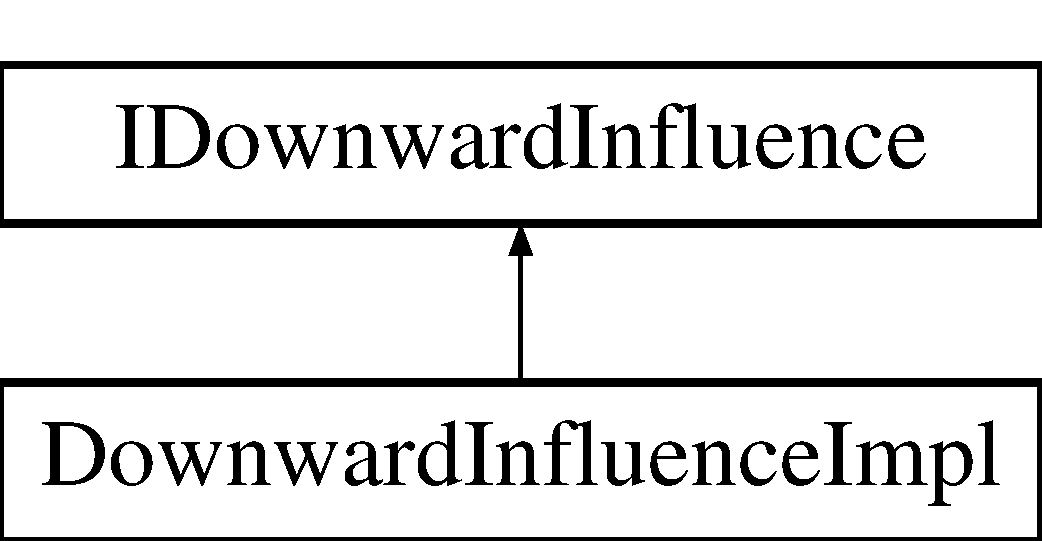
\includegraphics[height=2.000000cm]{classDownwardInfluenceImpl}
\end{center}
\end{figure}
\subsection*{Public Member Functions}
\begin{DoxyCompactItemize}
\item 
{\bfseries Downward\+Influence\+Impl} (\hyperlink{classNode}{Node} $\ast$node)\hypertarget{classDownwardInfluenceImpl_add04549a8e99e67304c133b4d9a46fc9}{}\label{classDownwardInfluenceImpl_add04549a8e99e67304c133b4d9a46fc9}

\item 
void {\bfseries calculate\+Downward\+Influence} ()\hypertarget{classDownwardInfluenceImpl_a05fdd6c5ef32911d503d9262e9431812}{}\label{classDownwardInfluenceImpl_a05fdd6c5ef32911d503d9262e9431812}

\end{DoxyCompactItemize}
\subsection*{Additional Inherited Members}


The documentation for this class was generated from the following files\+:\begin{DoxyCompactItemize}
\item 
/home/mate/\+Documents/\+Programming/\+Research/\+Multilayer\+Network\+Model/\+Multilayer\+Network\+Model/sources/core/\+Downward\+Influence/include/Downward\+Influence\+Impl.\+hh\item 
/home/mate/\+Documents/\+Programming/\+Research/\+Multilayer\+Network\+Model/\+Multilayer\+Network\+Model/sources/core/\+Downward\+Influence/src/Downward\+Influence\+Impl.\+cc\end{DoxyCompactItemize}

\hypertarget{classDynamicalEquation}{}\section{Dynamical\+Equation Class Reference}
\label{classDynamicalEquation}\index{Dynamical\+Equation@{Dynamical\+Equation}}
\subsection*{Public Member Functions}
\begin{DoxyCompactItemize}
\item 
double {\bfseries evaluate} ()\hypertarget{classDynamicalEquation_ac353d833e23a7718d28b48b96f273100}{}\label{classDynamicalEquation_ac353d833e23a7718d28b48b96f273100}

\item 
double {\bfseries evaluate\+At\+State} (std\+::map$<$ int, double $>$ starting\+State)\hypertarget{classDynamicalEquation_adf9454ebe570a95e2b4d72c04bdc82cc}{}\label{classDynamicalEquation_adf9454ebe570a95e2b4d72c04bdc82cc}

\item 
void {\bfseries O\+D\+Ecalculator} (const state\+\_\+type \&x, state\+\_\+type \&dxdt, double t)\hypertarget{classDynamicalEquation_a153f3c990807c596142b45d9f63ab57c}{}\label{classDynamicalEquation_a153f3c990807c596142b45d9f63ab57c}

\item 
void {\bfseries O\+D\+Ecalculator\+At\+State} (const state\+\_\+type \&x, state\+\_\+type \&dxdt, double t, std\+::map$<$ int, double $>$ starting\+State)\hypertarget{classDynamicalEquation_a07a6f24e0ca820c3734545c7d5d65927}{}\label{classDynamicalEquation_a07a6f24e0ca820c3734545c7d5d65927}

\item 
bool {\bfseries test\+Node\+Ids} (void) const \hypertarget{classDynamicalEquation_adbf7e8bad4b2764922b0ba2fe077b297}{}\label{classDynamicalEquation_adbf7e8bad4b2764922b0ba2fe077b297}

\item 
\hyperlink{classCalculationNode}{Calculation\+Node} $\ast$ {\bfseries get\+Base\+Calculation\+Node} (void)\hypertarget{classDynamicalEquation_aaa39d24b8dff72907638441db262c127}{}\label{classDynamicalEquation_aaa39d24b8dff72907638441db262c127}

\item 
void {\bfseries set\+Base\+Calculation\+Node} (\hyperlink{classCalculationNode}{Calculation\+Node} $\ast$base\+Calc\+Node)\hypertarget{classDynamicalEquation_a62f51fc853ccfa0aa2a09c3f2385eebe}{}\label{classDynamicalEquation_a62f51fc853ccfa0aa2a09c3f2385eebe}

\item 
void {\bfseries load\+Equation} (std\+::string str\+Equation)\hypertarget{classDynamicalEquation_aabe35a0aca2762081bd3b880f1648a87}{}\label{classDynamicalEquation_aabe35a0aca2762081bd3b880f1648a87}

\item 
void {\bfseries load\+Nodes\+To\+Equation} (\hyperlink{classCalculationNode}{Calculation\+Node} $\ast$calc\+Ptr, std\+::map$<$ int, \hyperlink{classNode}{Node} $\ast$ $>$ \&nodes\+Map)\hypertarget{classDynamicalEquation_a2c54698f5a05199a87ff0650836ff95c}{}\label{classDynamicalEquation_a2c54698f5a05199a87ff0650836ff95c}

\item 
std\+::string {\bfseries to\+String} () const \hypertarget{classDynamicalEquation_aed67e4c29392eb9c616b64acaa7500bc}{}\label{classDynamicalEquation_aed67e4c29392eb9c616b64acaa7500bc}

\end{DoxyCompactItemize}


The documentation for this class was generated from the following files\+:\begin{DoxyCompactItemize}
\item 
/home/mate/\+Documents/\+Programming/\+Research/\+Multilayer\+Network\+Model/\+Multilayer\+Network\+Model/src/core/include/Dynamical\+Equation.\+hh\item 
/home/mate/\+Documents/\+Programming/\+Research/\+Multilayer\+Network\+Model/\+Multilayer\+Network\+Model/src/core/src/Dynamical\+Equation.\+cc\end{DoxyCompactItemize}

\hypertarget{classDynamicalEquationGeneratorSimpleImpl}{}\section{Dynamical\+Equation\+Generator\+Simple\+Impl Class Reference}
\label{classDynamicalEquationGeneratorSimpleImpl}\index{Dynamical\+Equation\+Generator\+Simple\+Impl@{Dynamical\+Equation\+Generator\+Simple\+Impl}}
Inheritance diagram for Dynamical\+Equation\+Generator\+Simple\+Impl\+:\begin{figure}[H]
\begin{center}
\leavevmode
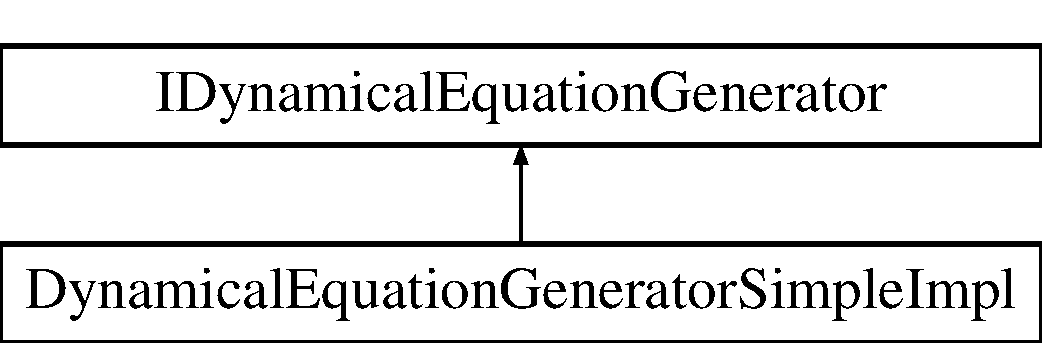
\includegraphics[height=2.000000cm]{classDynamicalEquationGeneratorSimpleImpl}
\end{center}
\end{figure}
\subsection*{Public Member Functions}
\begin{DoxyCompactItemize}
\item 
{\bfseries Dynamical\+Equation\+Generator\+Simple\+Impl} (\hyperlink{classMultilayerNetwork}{Multilayer\+Network} $\ast$multilayer\+Network)\hypertarget{classDynamicalEquationGeneratorSimpleImpl_aefe26119d2db680f1a03fc0b5415474e}{}\label{classDynamicalEquationGeneratorSimpleImpl_aefe26119d2db680f1a03fc0b5415474e}

\item 
void {\bfseries generate\+Dynamical\+Equations} ()\hypertarget{classDynamicalEquationGeneratorSimpleImpl_a92e9bade614a29d3c5351d89d43e98f1}{}\label{classDynamicalEquationGeneratorSimpleImpl_a92e9bade614a29d3c5351d89d43e98f1}

\end{DoxyCompactItemize}
\subsection*{Additional Inherited Members}


The documentation for this class was generated from the following files\+:\begin{DoxyCompactItemize}
\item 
/home/mate/\+Documents/\+Programming/\+Research/\+Multilayer\+Network\+Model/\+Multilayer\+Network\+Model/sources/generators/include/Dynamical\+Equation\+Generator\+Simple\+Impl.\+hh\item 
/home/mate/\+Documents/\+Programming/\+Research/\+Multilayer\+Network\+Model/\+Multilayer\+Network\+Model/sources/generators/src/Dynamical\+Equation\+Generator\+Simple\+Impl.\+cc\end{DoxyCompactItemize}

\hypertarget{classEncodedInputStream}{}\section{Encoded\+Input\+Stream$<$ Encoding, Input\+Byte\+Stream $>$ Class Template Reference}
\label{classEncodedInputStream}\index{Encoded\+Input\+Stream$<$ Encoding, Input\+Byte\+Stream $>$@{Encoded\+Input\+Stream$<$ Encoding, Input\+Byte\+Stream $>$}}


Input byte stream wrapper with a statically bound encoding.  




{\ttfamily \#include $<$encodedstream.\+h$>$}

\subsection*{Public Types}
\begin{DoxyCompactItemize}
\item 
typedef Encoding\+::\+Ch {\bfseries Ch}\hypertarget{classEncodedInputStream_acc387a1364390da244bbb1ab07bdceca}{}\label{classEncodedInputStream_acc387a1364390da244bbb1ab07bdceca}

\end{DoxyCompactItemize}
\subsection*{Public Member Functions}
\begin{DoxyCompactItemize}
\item 
{\bfseries Encoded\+Input\+Stream} (Input\+Byte\+Stream \&is)\hypertarget{classEncodedInputStream_a17f8e629500f6ae71cb72d1d63bf41fd}{}\label{classEncodedInputStream_a17f8e629500f6ae71cb72d1d63bf41fd}

\item 
Ch {\bfseries Peek} () const \hypertarget{classEncodedInputStream_abda3b0c141254343f4c481f67d52b423}{}\label{classEncodedInputStream_abda3b0c141254343f4c481f67d52b423}

\item 
Ch {\bfseries Take} ()\hypertarget{classEncodedInputStream_ab42cd57581bf62e42af471583e5b8377}{}\label{classEncodedInputStream_ab42cd57581bf62e42af471583e5b8377}

\item 
size\+\_\+t {\bfseries Tell} () const \hypertarget{classEncodedInputStream_a34cdb99fd81cd211f71903348e9c986f}{}\label{classEncodedInputStream_a34cdb99fd81cd211f71903348e9c986f}

\item 
void {\bfseries Put} (Ch)\hypertarget{classEncodedInputStream_afea36b666a44bd4adeabfcab7b68a322}{}\label{classEncodedInputStream_afea36b666a44bd4adeabfcab7b68a322}

\item 
void {\bfseries Flush} ()\hypertarget{classEncodedInputStream_aa4415bf4b97dd01e8c3de0ad7a161724}{}\label{classEncodedInputStream_aa4415bf4b97dd01e8c3de0ad7a161724}

\item 
Ch $\ast$ {\bfseries Put\+Begin} ()\hypertarget{classEncodedInputStream_ad97f7a549a8622c61b7fb2c63fedd69b}{}\label{classEncodedInputStream_ad97f7a549a8622c61b7fb2c63fedd69b}

\item 
size\+\_\+t {\bfseries Put\+End} (Ch $\ast$)\hypertarget{classEncodedInputStream_a83fe5ed281413d6005d1b324730e8bed}{}\label{classEncodedInputStream_a83fe5ed281413d6005d1b324730e8bed}

\end{DoxyCompactItemize}


\subsection{Detailed Description}
\subsubsection*{template$<$typename Encoding, typename Input\+Byte\+Stream$>$\\*
class Encoded\+Input\+Stream$<$ Encoding, Input\+Byte\+Stream $>$}

Input byte stream wrapper with a statically bound encoding. 


\begin{DoxyTemplParams}{Template Parameters}
{\em Encoding} & The interpretation of encoding of the stream. Either \hyperlink{structUTF8}{U\+T\+F8}, \hyperlink{structUTF16LE}{U\+T\+F16\+LE}, \hyperlink{structUTF16BE}{U\+T\+F16\+BE}, \hyperlink{structUTF32LE}{U\+T\+F32\+LE}, \hyperlink{structUTF32BE}{U\+T\+F32\+BE}. \\
\hline
{\em Input\+Byte\+Stream} & Type of input byte stream. For example, \hyperlink{classFileReadStream}{File\+Read\+Stream}. \\
\hline
\end{DoxyTemplParams}


The documentation for this class was generated from the following file\+:\begin{DoxyCompactItemize}
\item 
/home/mate/\+Documents/\+Programming/\+Research/\+Multilayer\+Network\+Model/\+Multilayer\+Network\+Model/src/external/rapidjson/encodedstream.\+h\end{DoxyCompactItemize}

\hypertarget{classEncodedInputStream_3_01UTF8_3_4_00_01MemoryStream_01_4}{}\section{Encoded\+Input\+Stream$<$ U\+T\+F8$<$$>$, Memory\+Stream $>$ Class Template Reference}
\label{classEncodedInputStream_3_01UTF8_3_4_00_01MemoryStream_01_4}\index{Encoded\+Input\+Stream$<$ U\+T\+F8$<$$>$, Memory\+Stream $>$@{Encoded\+Input\+Stream$<$ U\+T\+F8$<$$>$, Memory\+Stream $>$}}


Specialized for \hyperlink{structUTF8}{U\+T\+F8} \hyperlink{structMemoryStream}{Memory\+Stream}.  




{\ttfamily \#include $<$encodedstream.\+h$>$}

\subsection*{Public Types}
\begin{DoxyCompactItemize}
\item 
typedef U\+T\+F8\+::\+Ch {\bfseries Ch}\hypertarget{classEncodedInputStream_3_01UTF8_3_4_00_01MemoryStream_01_4_a091eb31dd2554bf10054148953f9b3bf}{}\label{classEncodedInputStream_3_01UTF8_3_4_00_01MemoryStream_01_4_a091eb31dd2554bf10054148953f9b3bf}

\end{DoxyCompactItemize}
\subsection*{Public Member Functions}
\begin{DoxyCompactItemize}
\item 
{\bfseries Encoded\+Input\+Stream} (\hyperlink{structMemoryStream}{Memory\+Stream} \&is)\hypertarget{classEncodedInputStream_3_01UTF8_3_4_00_01MemoryStream_01_4_a45ae1fa4f5bb8295df234fa3ac91ddef}{}\label{classEncodedInputStream_3_01UTF8_3_4_00_01MemoryStream_01_4_a45ae1fa4f5bb8295df234fa3ac91ddef}

\item 
Ch {\bfseries Peek} () const \hypertarget{classEncodedInputStream_3_01UTF8_3_4_00_01MemoryStream_01_4_aecd5a2355826e77f7958a26b5449ee62}{}\label{classEncodedInputStream_3_01UTF8_3_4_00_01MemoryStream_01_4_aecd5a2355826e77f7958a26b5449ee62}

\item 
Ch {\bfseries Take} ()\hypertarget{classEncodedInputStream_3_01UTF8_3_4_00_01MemoryStream_01_4_a29eeabe922bb6c7cbb5c16fe8a3a7859}{}\label{classEncodedInputStream_3_01UTF8_3_4_00_01MemoryStream_01_4_a29eeabe922bb6c7cbb5c16fe8a3a7859}

\item 
size\+\_\+t {\bfseries Tell} () const \hypertarget{classEncodedInputStream_3_01UTF8_3_4_00_01MemoryStream_01_4_a8473e37416580962d8d491350c9fab2b}{}\label{classEncodedInputStream_3_01UTF8_3_4_00_01MemoryStream_01_4_a8473e37416580962d8d491350c9fab2b}

\item 
void {\bfseries Put} (Ch)\hypertarget{classEncodedInputStream_3_01UTF8_3_4_00_01MemoryStream_01_4_a39fe296cfa45d7f8ef5adc0dd30036c2}{}\label{classEncodedInputStream_3_01UTF8_3_4_00_01MemoryStream_01_4_a39fe296cfa45d7f8ef5adc0dd30036c2}

\item 
void {\bfseries Flush} ()\hypertarget{classEncodedInputStream_3_01UTF8_3_4_00_01MemoryStream_01_4_ad911c889ebd4ded9bcf9d31ca124f9a7}{}\label{classEncodedInputStream_3_01UTF8_3_4_00_01MemoryStream_01_4_ad911c889ebd4ded9bcf9d31ca124f9a7}

\item 
Ch $\ast$ {\bfseries Put\+Begin} ()\hypertarget{classEncodedInputStream_3_01UTF8_3_4_00_01MemoryStream_01_4_a3ca21c33ccc4a12fe2f806b865bd3ebd}{}\label{classEncodedInputStream_3_01UTF8_3_4_00_01MemoryStream_01_4_a3ca21c33ccc4a12fe2f806b865bd3ebd}

\item 
size\+\_\+t {\bfseries Put\+End} (Ch $\ast$)\hypertarget{classEncodedInputStream_3_01UTF8_3_4_00_01MemoryStream_01_4_ad87990d605c72529aeb78509d5b393fb}{}\label{classEncodedInputStream_3_01UTF8_3_4_00_01MemoryStream_01_4_ad87990d605c72529aeb78509d5b393fb}

\end{DoxyCompactItemize}
\subsection*{Public Attributes}
\begin{DoxyCompactItemize}
\item 
\hyperlink{structMemoryStream}{Memory\+Stream} \& {\bfseries is\+\_\+}\hypertarget{classEncodedInputStream_3_01UTF8_3_4_00_01MemoryStream_01_4_ad5e48564bbd14297a4cc445af3a4aa83}{}\label{classEncodedInputStream_3_01UTF8_3_4_00_01MemoryStream_01_4_ad5e48564bbd14297a4cc445af3a4aa83}

\end{DoxyCompactItemize}


\subsection{Detailed Description}
\subsubsection*{template$<$$>$\\*
class Encoded\+Input\+Stream$<$ U\+T\+F8$<$$>$, Memory\+Stream $>$}

Specialized for \hyperlink{structUTF8}{U\+T\+F8} \hyperlink{structMemoryStream}{Memory\+Stream}. 

The documentation for this class was generated from the following file\+:\begin{DoxyCompactItemize}
\item 
/home/mate/\+Documents/\+Programming/\+Research/\+Multilayer\+Network\+Model/\+Multilayer\+Network\+Model/src/external/rapidjson/encodedstream.\+h\end{DoxyCompactItemize}

\hypertarget{classEncodedOutputStream}{}\section{Encoded\+Output\+Stream$<$ Encoding, Output\+Byte\+Stream $>$ Class Template Reference}
\label{classEncodedOutputStream}\index{Encoded\+Output\+Stream$<$ Encoding, Output\+Byte\+Stream $>$@{Encoded\+Output\+Stream$<$ Encoding, Output\+Byte\+Stream $>$}}


Output byte stream wrapper with statically bound encoding.  




{\ttfamily \#include $<$encodedstream.\+h$>$}

\subsection*{Public Types}
\begin{DoxyCompactItemize}
\item 
typedef Encoding\+::\+Ch {\bfseries Ch}\hypertarget{classEncodedOutputStream_aa8f494d7ee2808307fbc9cd658c0f760}{}\label{classEncodedOutputStream_aa8f494d7ee2808307fbc9cd658c0f760}

\end{DoxyCompactItemize}
\subsection*{Public Member Functions}
\begin{DoxyCompactItemize}
\item 
{\bfseries Encoded\+Output\+Stream} (Output\+Byte\+Stream \&os, bool put\+B\+OM=true)\hypertarget{classEncodedOutputStream_ad3360c613a30a6a15526ae9ad63bd004}{}\label{classEncodedOutputStream_ad3360c613a30a6a15526ae9ad63bd004}

\item 
void {\bfseries Put} (Ch c)\hypertarget{classEncodedOutputStream_a0f3c00f94c195a38d78c05ecda497481}{}\label{classEncodedOutputStream_a0f3c00f94c195a38d78c05ecda497481}

\item 
void {\bfseries Flush} ()\hypertarget{classEncodedOutputStream_a657188f6a9f0fae01a4012c288d3fd46}{}\label{classEncodedOutputStream_a657188f6a9f0fae01a4012c288d3fd46}

\item 
Ch {\bfseries Peek} () const \hypertarget{classEncodedOutputStream_aa1dbe6b921fe788f3229024fb5598647}{}\label{classEncodedOutputStream_aa1dbe6b921fe788f3229024fb5598647}

\item 
Ch {\bfseries Take} ()\hypertarget{classEncodedOutputStream_a90f5a5e1598316a417ef5b6ad3d49f36}{}\label{classEncodedOutputStream_a90f5a5e1598316a417ef5b6ad3d49f36}

\item 
size\+\_\+t {\bfseries Tell} () const \hypertarget{classEncodedOutputStream_ab580ac97f1a22c2a6abc4a31bb5c8272}{}\label{classEncodedOutputStream_ab580ac97f1a22c2a6abc4a31bb5c8272}

\item 
Ch $\ast$ {\bfseries Put\+Begin} ()\hypertarget{classEncodedOutputStream_a78934de4f76c9fa65238e65d3630cbc5}{}\label{classEncodedOutputStream_a78934de4f76c9fa65238e65d3630cbc5}

\item 
size\+\_\+t {\bfseries Put\+End} (Ch $\ast$)\hypertarget{classEncodedOutputStream_a818695f6d3fa8896e9d7d0fbdc7d4514}{}\label{classEncodedOutputStream_a818695f6d3fa8896e9d7d0fbdc7d4514}

\end{DoxyCompactItemize}


\subsection{Detailed Description}
\subsubsection*{template$<$typename Encoding, typename Output\+Byte\+Stream$>$\\*
class Encoded\+Output\+Stream$<$ Encoding, Output\+Byte\+Stream $>$}

Output byte stream wrapper with statically bound encoding. 


\begin{DoxyTemplParams}{Template Parameters}
{\em Encoding} & The interpretation of encoding of the stream. Either \hyperlink{structUTF8}{U\+T\+F8}, \hyperlink{structUTF16LE}{U\+T\+F16\+LE}, \hyperlink{structUTF16BE}{U\+T\+F16\+BE}, \hyperlink{structUTF32LE}{U\+T\+F32\+LE}, \hyperlink{structUTF32BE}{U\+T\+F32\+BE}. \\
\hline
{\em Output\+Byte\+Stream} & Type of input byte stream. For example, \hyperlink{classFileWriteStream}{File\+Write\+Stream}. \\
\hline
\end{DoxyTemplParams}


The documentation for this class was generated from the following file\+:\begin{DoxyCompactItemize}
\item 
/home/mate/\+Documents/\+Programming/\+Research/\+Multilayer\+Network\+Model/\+Multilayer\+Network\+Model/sources/external/rapidjson/encodedstream.\+h\end{DoxyCompactItemize}

\hypertarget{classrapidjson_1_1Encoding}{}\section{rapidjson\+:\+:Encoding Class Reference}
\label{classrapidjson_1_1Encoding}\index{rapidjson\+::\+Encoding@{rapidjson\+::\+Encoding}}


Concept for encoding of Unicode characters.  




{\ttfamily \#include $<$encodings.\+h$>$}



\subsection{Detailed Description}
Concept for encoding of Unicode characters. 


\begin{DoxyCode}
concept Encoding \{
    \textcolor{keyword}{typename} Ch;    

    \textcolor{keyword}{enum} \{ supportUnicode = 1 \}; \textcolor{comment}{// or 0 if not supporting unicode}

    \textcolor{keyword}{template}<\textcolor{keyword}{typename} OutputStream>
    \textcolor{keyword}{static} \textcolor{keywordtype}{void} Encode(OutputStream& os, \textcolor{keywordtype}{unsigned} codepoint);

    \textcolor{keyword}{template} <\textcolor{keyword}{typename} InputStream>
    \textcolor{keyword}{static} \textcolor{keywordtype}{bool} Decode(InputStream& is, \textcolor{keywordtype}{unsigned}* codepoint);

    \textcolor{keyword}{template} <\textcolor{keyword}{typename} InputStream, \textcolor{keyword}{typename} OutputStream>
    \textcolor{keyword}{static} \textcolor{keywordtype}{bool} Validate(InputStream& is, OutputStream& os);

    \textcolor{comment}{// The following functions are deal with byte streams.}

    \textcolor{keyword}{template} <\textcolor{keyword}{typename} InputByteStream>
    \textcolor{keyword}{static} CharType TakeBOM(InputByteStream& is);

    \textcolor{keyword}{template} <\textcolor{keyword}{typename} InputByteStream>
    \textcolor{keyword}{static} Ch Take(InputByteStream& is);

    \textcolor{keyword}{template} <\textcolor{keyword}{typename} OutputByteStream>
    \textcolor{keyword}{static} \textcolor{keywordtype}{void} PutBOM(OutputByteStream& os);

    \textcolor{keyword}{template} <\textcolor{keyword}{typename} OutputByteStream>
    \textcolor{keyword}{static} \textcolor{keywordtype}{void} Put(OutputByteStream& os, Ch c);
\};
\end{DoxyCode}
 

The documentation for this class was generated from the following file\+:\begin{DoxyCompactItemize}
\item 
/home/mate/\+Documents/\+Programming/\+Research/\+Multilayer\+Network\+Model/\+Multilayer\+Network\+Model/src/external/rapidjson/encodings.\+h\end{DoxyCompactItemize}

\hypertarget{classFileReadStream}{}\section{File\+Read\+Stream Class Reference}
\label{classFileReadStream}\index{File\+Read\+Stream@{File\+Read\+Stream}}


File byte stream for input using fread().  




{\ttfamily \#include $<$filereadstream.\+h$>$}

\subsection*{Public Types}
\begin{DoxyCompactItemize}
\item 
typedef char \hyperlink{classFileReadStream_ae1f83d9ca3c76d1d151af0b6c427f046}{Ch}\hypertarget{classFileReadStream_ae1f83d9ca3c76d1d151af0b6c427f046}{}\label{classFileReadStream_ae1f83d9ca3c76d1d151af0b6c427f046}

\begin{DoxyCompactList}\small\item\em Character type (byte). \end{DoxyCompactList}\end{DoxyCompactItemize}
\subsection*{Public Member Functions}
\begin{DoxyCompactItemize}
\item 
\hyperlink{classFileReadStream_adf91191843d50b900f43cb4f35f16f67}{File\+Read\+Stream} (std\+::\+F\+I\+LE $\ast$fp, char $\ast$buffer, size\+\_\+t buffer\+Size)
\begin{DoxyCompactList}\small\item\em Constructor. \end{DoxyCompactList}\item 
\hyperlink{classFileReadStream_ae1f83d9ca3c76d1d151af0b6c427f046}{Ch} {\bfseries Peek} () const \hypertarget{classFileReadStream_ab129c5d15343488caf60b4fee48024fb}{}\label{classFileReadStream_ab129c5d15343488caf60b4fee48024fb}

\item 
\hyperlink{classFileReadStream_ae1f83d9ca3c76d1d151af0b6c427f046}{Ch} {\bfseries Take} ()\hypertarget{classFileReadStream_addcbccc9d86ccbbe6d8e876ba595dbcb}{}\label{classFileReadStream_addcbccc9d86ccbbe6d8e876ba595dbcb}

\item 
size\+\_\+t {\bfseries Tell} () const \hypertarget{classFileReadStream_a9a2f09eb66ae912c4d5f472bdfdd92ce}{}\label{classFileReadStream_a9a2f09eb66ae912c4d5f472bdfdd92ce}

\item 
void {\bfseries Put} (\hyperlink{classFileReadStream_ae1f83d9ca3c76d1d151af0b6c427f046}{Ch})\hypertarget{classFileReadStream_a4f2eac5b08033b1527bff517be657a36}{}\label{classFileReadStream_a4f2eac5b08033b1527bff517be657a36}

\item 
void {\bfseries Flush} ()\hypertarget{classFileReadStream_acd031e3f578b23bc2a792ac41e1e95ae}{}\label{classFileReadStream_acd031e3f578b23bc2a792ac41e1e95ae}

\item 
\hyperlink{classFileReadStream_ae1f83d9ca3c76d1d151af0b6c427f046}{Ch} $\ast$ {\bfseries Put\+Begin} ()\hypertarget{classFileReadStream_ac985850ab75f204dc08a01d12a8ef5c6}{}\label{classFileReadStream_ac985850ab75f204dc08a01d12a8ef5c6}

\item 
size\+\_\+t {\bfseries Put\+End} (\hyperlink{classFileReadStream_ae1f83d9ca3c76d1d151af0b6c427f046}{Ch} $\ast$)\hypertarget{classFileReadStream_a886660c89f698ff913d641d61466108f}{}\label{classFileReadStream_a886660c89f698ff913d641d61466108f}

\item 
const \hyperlink{classFileReadStream_ae1f83d9ca3c76d1d151af0b6c427f046}{Ch} $\ast$ {\bfseries Peek4} () const \hypertarget{classFileReadStream_a33ebc2af3a7dea770c70e9c1d53f0f91}{}\label{classFileReadStream_a33ebc2af3a7dea770c70e9c1d53f0f91}

\end{DoxyCompactItemize}


\subsection{Detailed Description}
File byte stream for input using fread(). 

\begin{DoxyNote}{Note}
implements Stream concept 
\end{DoxyNote}


\subsection{Constructor \& Destructor Documentation}
\index{File\+Read\+Stream@{File\+Read\+Stream}!File\+Read\+Stream@{File\+Read\+Stream}}
\index{File\+Read\+Stream@{File\+Read\+Stream}!File\+Read\+Stream@{File\+Read\+Stream}}
\subsubsection[{\texorpdfstring{File\+Read\+Stream(std\+::\+F\+I\+L\+E $\ast$fp, char $\ast$buffer, size\+\_\+t buffer\+Size)}{FileReadStream(std::FILE *fp, char *buffer, size_t bufferSize)}}]{\setlength{\rightskip}{0pt plus 5cm}File\+Read\+Stream\+::\+File\+Read\+Stream (
\begin{DoxyParamCaption}
\item[{std\+::\+F\+I\+LE $\ast$}]{fp, }
\item[{char $\ast$}]{buffer, }
\item[{size\+\_\+t}]{buffer\+Size}
\end{DoxyParamCaption}
)\hspace{0.3cm}{\ttfamily [inline]}}\hypertarget{classFileReadStream_adf91191843d50b900f43cb4f35f16f67}{}\label{classFileReadStream_adf91191843d50b900f43cb4f35f16f67}


Constructor. 


\begin{DoxyParams}{Parameters}
{\em fp} & File pointer opened for read. \\
\hline
{\em buffer} & user-\/supplied buffer. \\
\hline
{\em buffer\+Size} & size of buffer in bytes. Must $>$=4 bytes. \\
\hline
\end{DoxyParams}


The documentation for this class was generated from the following file\+:\begin{DoxyCompactItemize}
\item 
/home/mate/\+Documents/\+Programming/\+Research/\+Multilayer\+Network\+Model/\+Multilayer\+Network\+Model/sources/external/rapidjson/filereadstream.\+h\end{DoxyCompactItemize}

\hypertarget{classFileWriteStream}{}\section{File\+Write\+Stream Class Reference}
\label{classFileWriteStream}\index{File\+Write\+Stream@{File\+Write\+Stream}}


Wrapper of C file stream for input using fread().  




{\ttfamily \#include $<$filewritestream.\+h$>$}

\subsection*{Public Types}
\begin{DoxyCompactItemize}
\item 
typedef char \hyperlink{classFileWriteStream_abc16aeb69ad4176263ddfcb837fb7b49}{Ch}\hypertarget{classFileWriteStream_abc16aeb69ad4176263ddfcb837fb7b49}{}\label{classFileWriteStream_abc16aeb69ad4176263ddfcb837fb7b49}

\begin{DoxyCompactList}\small\item\em Character type. Only support char. \end{DoxyCompactList}\end{DoxyCompactItemize}
\subsection*{Public Member Functions}
\begin{DoxyCompactItemize}
\item 
{\bfseries File\+Write\+Stream} (std\+::\+F\+I\+LE $\ast$fp, char $\ast$buffer, size\+\_\+t buffer\+Size)\hypertarget{classFileWriteStream_a553ea3e7377a7f7cace2daa3cc90e1a1}{}\label{classFileWriteStream_a553ea3e7377a7f7cace2daa3cc90e1a1}

\item 
void {\bfseries Put} (char c)\hypertarget{classFileWriteStream_af6a6061d0accd939fa475b9b34427d85}{}\label{classFileWriteStream_af6a6061d0accd939fa475b9b34427d85}

\item 
void {\bfseries PutN} (char c, size\+\_\+t n)\hypertarget{classFileWriteStream_ad9ec108b24316a2c1c83c6ddc75d308a}{}\label{classFileWriteStream_ad9ec108b24316a2c1c83c6ddc75d308a}

\item 
void {\bfseries Flush} ()\hypertarget{classFileWriteStream_a939fbf183ba36464c5e0837df4329d37}{}\label{classFileWriteStream_a939fbf183ba36464c5e0837df4329d37}

\item 
char {\bfseries Peek} () const \hypertarget{classFileWriteStream_a83a8321c33738544f05330f3638e51c0}{}\label{classFileWriteStream_a83a8321c33738544f05330f3638e51c0}

\item 
char {\bfseries Take} ()\hypertarget{classFileWriteStream_ac927a0ae09a85eaba58a74ceb04b40ed}{}\label{classFileWriteStream_ac927a0ae09a85eaba58a74ceb04b40ed}

\item 
size\+\_\+t {\bfseries Tell} () const \hypertarget{classFileWriteStream_a72889b68dbd766cea0e003389b990722}{}\label{classFileWriteStream_a72889b68dbd766cea0e003389b990722}

\item 
char $\ast$ {\bfseries Put\+Begin} ()\hypertarget{classFileWriteStream_a4d1340a64fde3f16ac2afce19537c75e}{}\label{classFileWriteStream_a4d1340a64fde3f16ac2afce19537c75e}

\item 
size\+\_\+t {\bfseries Put\+End} (char $\ast$)\hypertarget{classFileWriteStream_a54b14047e4c998db0594290605f8f0dc}{}\label{classFileWriteStream_a54b14047e4c998db0594290605f8f0dc}

\end{DoxyCompactItemize}


\subsection{Detailed Description}
Wrapper of C file stream for input using fread(). 

\begin{DoxyNote}{Note}
implements Stream concept 
\end{DoxyNote}


The documentation for this class was generated from the following file\+:\begin{DoxyCompactItemize}
\item 
/home/mate/\+Documents/\+Programming/\+Research/\+Multilayer\+Network\+Model/\+Multilayer\+Network\+Model/sources/external/rapidjson/filewritestream.\+h\end{DoxyCompactItemize}

\hypertarget{structGenericValue_1_1Flag}{}\section{Generic\+Value$<$ Encoding, Allocator $>$\+:\+:Flag Struct Reference}
\label{structGenericValue_1_1Flag}\index{Generic\+Value$<$ Encoding, Allocator $>$\+::\+Flag@{Generic\+Value$<$ Encoding, Allocator $>$\+::\+Flag}}
\subsection*{Public Attributes}
\begin{DoxyCompactItemize}
\item 
char {\bfseries payload} \mbox{[}sizeof(\hyperlink{rapidjson_8h_a5ed6e6e67250fadbd041127e6386dcb5}{Size\+Type})$\ast$2+sizeof(void $\ast$)+2\mbox{]}\hypertarget{structGenericValue_1_1Flag_ac5512252dcb1f2e4b0231dbde504c656}{}\label{structGenericValue_1_1Flag_ac5512252dcb1f2e4b0231dbde504c656}

\item 
uint16\+\_\+t {\bfseries flags}\hypertarget{structGenericValue_1_1Flag_ac91f08067dcc0003fc78e870ca9b2d5d}{}\label{structGenericValue_1_1Flag_ac91f08067dcc0003fc78e870ca9b2d5d}

\end{DoxyCompactItemize}


The documentation for this struct was generated from the following file\+:\begin{DoxyCompactItemize}
\item 
/home/mate/\+Documents/\+Programming/\+Research/\+Multilayer\+Network\+Model/\+Multilayer\+Network\+Model/src/external/rapidjson/\hyperlink{document_8h}{document.\+h}\end{DoxyCompactItemize}

\hypertarget{classGenericArray}{}\section{Generic\+Array$<$ Const, ValueT $>$ Class Template Reference}
\label{classGenericArray}\index{Generic\+Array$<$ Const, Value\+T $>$@{Generic\+Array$<$ Const, Value\+T $>$}}


Helper class for accessing Value of array type.  




{\ttfamily \#include $<$document.\+h$>$}

\subsection*{Public Types}
\begin{DoxyCompactItemize}
\item 
typedef \hyperlink{classGenericArray}{Generic\+Array}$<$ true, ValueT $>$ {\bfseries Const\+Array}\hypertarget{classGenericArray_a84f0b14518bc5cc44b4ff76a7d5ef81b}{}\label{classGenericArray_a84f0b14518bc5cc44b4ff76a7d5ef81b}

\item 
typedef \hyperlink{classGenericArray}{Generic\+Array}$<$ false, ValueT $>$ {\bfseries Array}\hypertarget{classGenericArray_a6683902e86c051c2319e873537dca7b1}{}\label{classGenericArray_a6683902e86c051c2319e873537dca7b1}

\item 
typedef ValueT {\bfseries Plain\+Type}\hypertarget{classGenericArray_aecea8be3dca6799bc523f4bffd221839}{}\label{classGenericArray_aecea8be3dca6799bc523f4bffd221839}

\item 
typedef internal\+::\+Maybe\+Add\+Const$<$ Const, Plain\+Type $>$\+::\hyperlink{rapidjson_8h_a1d1cfd8ffb84e947f82999c682b666a7}{Type} {\bfseries Value\+Type}\hypertarget{classGenericArray_a93e53f38a99fc5167eb2a28653de64ed}{}\label{classGenericArray_a93e53f38a99fc5167eb2a28653de64ed}

\item 
typedef Value\+Type $\ast$ {\bfseries Value\+Iterator}\hypertarget{classGenericArray_afc6ad62c3f00531fa378db266182704a}{}\label{classGenericArray_afc6ad62c3f00531fa378db266182704a}

\item 
typedef const ValueT $\ast$ {\bfseries Const\+Value\+Iterator}\hypertarget{classGenericArray_a1cd7bb3e75ccfeed3e8b0a6bb5563d68}{}\label{classGenericArray_a1cd7bb3e75ccfeed3e8b0a6bb5563d68}

\item 
typedef Value\+Type\+::\+Allocator\+Type {\bfseries Allocator\+Type}\hypertarget{classGenericArray_af9cdc12de03c742b9c33dfc172756b97}{}\label{classGenericArray_af9cdc12de03c742b9c33dfc172756b97}

\item 
typedef Value\+Type\+::\+String\+Ref\+Type {\bfseries String\+Ref\+Type}\hypertarget{classGenericArray_a8dcb9e2a2e103ce1051c16a7486465b9}{}\label{classGenericArray_a8dcb9e2a2e103ce1051c16a7486465b9}

\end{DoxyCompactItemize}
\subsection*{Public Member Functions}
\begin{DoxyCompactItemize}
\item 
{\bfseries Generic\+Array} (const \hyperlink{classGenericArray}{Generic\+Array} \&rhs)\hypertarget{classGenericArray_aa589d897a194b349d5053391a6f1491d}{}\label{classGenericArray_aa589d897a194b349d5053391a6f1491d}

\item 
\hyperlink{classGenericArray}{Generic\+Array} \& {\bfseries operator=} (const \hyperlink{classGenericArray}{Generic\+Array} \&rhs)\hypertarget{classGenericArray_addbff152092d0998b2c550bd575f4b83}{}\label{classGenericArray_addbff152092d0998b2c550bd575f4b83}

\item 
\hyperlink{rapidjson_8h_a5ed6e6e67250fadbd041127e6386dcb5}{Size\+Type} {\bfseries Size} () const \hypertarget{classGenericArray_a9666a5feb3fccbcec330b53742d00371}{}\label{classGenericArray_a9666a5feb3fccbcec330b53742d00371}

\item 
\hyperlink{rapidjson_8h_a5ed6e6e67250fadbd041127e6386dcb5}{Size\+Type} {\bfseries Capacity} () const \hypertarget{classGenericArray_a12717a6bcd3949dea08ae19a9e940d58}{}\label{classGenericArray_a12717a6bcd3949dea08ae19a9e940d58}

\item 
bool {\bfseries Empty} () const \hypertarget{classGenericArray_a85c783f2f31684901cc2fbf178b1aba5}{}\label{classGenericArray_a85c783f2f31684901cc2fbf178b1aba5}

\item 
void {\bfseries Clear} () const \hypertarget{classGenericArray_a9a67311453f8941f0ac1b5471ec6b99f}{}\label{classGenericArray_a9a67311453f8941f0ac1b5471ec6b99f}

\item 
Value\+Type \& {\bfseries operator\mbox{[}$\,$\mbox{]}} (\hyperlink{rapidjson_8h_a5ed6e6e67250fadbd041127e6386dcb5}{Size\+Type} index) const \hypertarget{classGenericArray_ac928627968bcfff4746f04c2cdd103ef}{}\label{classGenericArray_ac928627968bcfff4746f04c2cdd103ef}

\item 
Value\+Iterator {\bfseries Begin} () const \hypertarget{classGenericArray_a04cb899ae93f89ba91fab09381d731d3}{}\label{classGenericArray_a04cb899ae93f89ba91fab09381d731d3}

\item 
Value\+Iterator {\bfseries End} () const \hypertarget{classGenericArray_aa75006f979b2d810e6ab0ff4f755cf32}{}\label{classGenericArray_aa75006f979b2d810e6ab0ff4f755cf32}

\item 
\hyperlink{classGenericArray}{Generic\+Array} {\bfseries Reserve} (\hyperlink{rapidjson_8h_a5ed6e6e67250fadbd041127e6386dcb5}{Size\+Type} new\+Capacity, Allocator\+Type \&allocator) const \hypertarget{classGenericArray_affe36316cbe3f80ece8a6fc45b777a58}{}\label{classGenericArray_affe36316cbe3f80ece8a6fc45b777a58}

\item 
\hyperlink{classGenericArray}{Generic\+Array} {\bfseries Push\+Back} (Value\+Type \&value, Allocator\+Type \&allocator) const \hypertarget{classGenericArray_a6aad4336bb87edc9113f34a6d9073d53}{}\label{classGenericArray_a6aad4336bb87edc9113f34a6d9073d53}

\item 
\hyperlink{classGenericArray}{Generic\+Array} {\bfseries Push\+Back} (String\+Ref\+Type value, Allocator\+Type \&allocator) const \hypertarget{classGenericArray_af583610a94a0fe360a5cbfd34fe8aa6c}{}\label{classGenericArray_af583610a94a0fe360a5cbfd34fe8aa6c}

\item 
{\footnotesize template$<$typename T $>$ }\\{\bfseries R\+A\+P\+I\+D\+J\+S\+O\+N\+\_\+\+D\+I\+S\+A\+B\+L\+E\+I\+F\+\_\+\+R\+E\+T\+U\+RN} ((internal\+::\+Or\+Expr$<$ internal\+::\+Is\+Pointer$<$ T $>$, \hyperlink{structinternal_1_1IsGenericValue}{internal\+::\+Is\+Generic\+Value}$<$ T $>$ $>$),(const \hyperlink{classGenericArray}{Generic\+Array} \&)) Push\+Back(T value\hypertarget{classGenericArray_a12adff0c1e11aa3be6f4160015a65df0}{}\label{classGenericArray_a12adff0c1e11aa3be6f4160015a65df0}

\item 
\hyperlink{classGenericArray}{Generic\+Array} {\bfseries Pop\+Back} () const \hypertarget{classGenericArray_a87a5a9acf7b26a81df42a54553bdbec4}{}\label{classGenericArray_a87a5a9acf7b26a81df42a54553bdbec4}

\item 
Value\+Iterator {\bfseries Erase} (Const\+Value\+Iterator pos) const \hypertarget{classGenericArray_a1d71be1384a0184514d9921d77b6a060}{}\label{classGenericArray_a1d71be1384a0184514d9921d77b6a060}

\item 
Value\+Iterator {\bfseries Erase} (Const\+Value\+Iterator first, Const\+Value\+Iterator last) const \hypertarget{classGenericArray_a105cb20275127cbd73fbc24e6af41dd1}{}\label{classGenericArray_a105cb20275127cbd73fbc24e6af41dd1}

\end{DoxyCompactItemize}
\subsection*{Public Attributes}
\begin{DoxyCompactItemize}
\item 
Allocator\+Type \&allocator {\bfseries const} \{ value\+\_\+.\+Push\+Back(value, allocator)\hypertarget{classGenericArray_a25d2ed55daa117c41db6a5b3f87e9ddc}{}\label{classGenericArray_a25d2ed55daa117c41db6a5b3f87e9ddc}

\item 
return $\ast$ {\bfseries this}\hypertarget{classGenericArray_aef8b7baa9ec5cd68d8951fa8bad85217}{}\label{classGenericArray_aef8b7baa9ec5cd68d8951fa8bad85217}

\end{DoxyCompactItemize}
\subsection*{Friends}
\begin{DoxyCompactItemize}
\item 
{\footnotesize template$<$typename , typename $>$ }\\class {\bfseries Generic\+Value}\hypertarget{classGenericArray_a899449e1a645b5e377af059fb61113d8}{}\label{classGenericArray_a899449e1a645b5e377af059fb61113d8}

\end{DoxyCompactItemize}


\subsection{Detailed Description}
\subsubsection*{template$<$bool Const, typename ValueT$>$\\*
class Generic\+Array$<$ Const, Value\+T $>$}

Helper class for accessing Value of array type. 

Instance of this helper class is obtained by {\ttfamily Generic\+Value\+::\+Get\+Array()}. In addition to all A\+P\+Is for array type, it provides range-\/based for loop if {\ttfamily R\+A\+P\+I\+D\+J\+S\+O\+N\+\_\+\+H\+A\+S\+\_\+\+C\+X\+X11\+\_\+\+R\+A\+N\+G\+E\+\_\+\+F\+OR=1}. 

The documentation for this class was generated from the following file\+:\begin{DoxyCompactItemize}
\item 
/home/mate/\+Documents/\+Programming/\+Research/\+Multilayer\+Network\+Model/\+Multilayer\+Network\+Model/src/external/rapidjson/\hyperlink{document_8h}{document.\+h}\end{DoxyCompactItemize}

\hypertarget{classGenericDocument}{}\section{Generic\+Document$<$ Encoding, Allocator, Stack\+Allocator $>$ Class Template Reference}
\label{classGenericDocument}\index{Generic\+Document$<$ Encoding, Allocator, Stack\+Allocator $>$@{Generic\+Document$<$ Encoding, Allocator, Stack\+Allocator $>$}}


A document for parsing J\+S\+ON text as D\+OM.  




{\ttfamily \#include $<$document.\+h$>$}

Inheritance diagram for Generic\+Document$<$ Encoding, Allocator, Stack\+Allocator $>$\+:\begin{figure}[H]
\begin{center}
\leavevmode
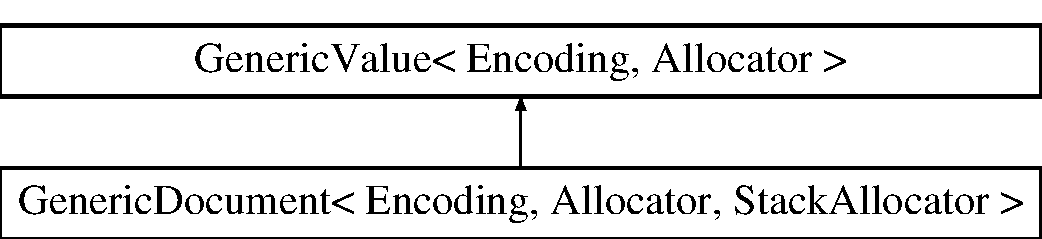
\includegraphics[height=2.000000cm]{classGenericDocument}
\end{center}
\end{figure}
\subsection*{Public Types}
\begin{DoxyCompactItemize}
\item 
typedef Encoding\+::\+Ch \hyperlink{classGenericDocument_a6f5b0b7b6626508d094ae67490269700}{Ch}\hypertarget{classGenericDocument_a6f5b0b7b6626508d094ae67490269700}{}\label{classGenericDocument_a6f5b0b7b6626508d094ae67490269700}

\begin{DoxyCompactList}\small\item\em Character type derived from Encoding. \end{DoxyCompactList}\item 
typedef \hyperlink{classGenericValue}{Generic\+Value}$<$ Encoding, Allocator $>$ \hyperlink{classGenericDocument_a8936205dc215dda029060d7e835e0549}{Value\+Type}\hypertarget{classGenericDocument_a8936205dc215dda029060d7e835e0549}{}\label{classGenericDocument_a8936205dc215dda029060d7e835e0549}

\begin{DoxyCompactList}\small\item\em Value type of the document. \end{DoxyCompactList}\item 
typedef Allocator \hyperlink{classGenericDocument_a35155b912da66ced38d22e2551364c57}{Allocator\+Type}\hypertarget{classGenericDocument_a35155b912da66ced38d22e2551364c57}{}\label{classGenericDocument_a35155b912da66ced38d22e2551364c57}

\begin{DoxyCompactList}\small\item\em Allocator type from template parameter. \end{DoxyCompactList}\end{DoxyCompactItemize}
\subsection*{Public Member Functions}
\begin{DoxyCompactItemize}
\item 
\hyperlink{classGenericDocument_a3da21e72ec8f26b9da77d86cc1d41cdd}{Generic\+Document} (\hyperlink{rapidjson_8h_a1d1cfd8ffb84e947f82999c682b666a7}{Type} type, Allocator $\ast$allocator=0, size\+\_\+t stack\+Capacity=k\+Default\+Stack\+Capacity, Stack\+Allocator $\ast$stack\+Allocator=0)
\begin{DoxyCompactList}\small\item\em Constructor. \end{DoxyCompactList}\item 
\hyperlink{classGenericDocument_a6b1c313ad538cafc4d23d4bd5f97178c}{Generic\+Document} (Allocator $\ast$allocator=0, size\+\_\+t stack\+Capacity=k\+Default\+Stack\+Capacity, Stack\+Allocator $\ast$stack\+Allocator=0)
\begin{DoxyCompactList}\small\item\em Constructor. \end{DoxyCompactList}\item 
\hyperlink{classGenericDocument}{Generic\+Document} \& \hyperlink{classGenericDocument_a6290e1290fad74177625af5938c0c58f}{Swap} (\hyperlink{classGenericDocument}{Generic\+Document} \&rhs) R\+A\+P\+I\+D\+J\+S\+O\+N\+\_\+\+N\+O\+E\+X\+C\+E\+PT
\begin{DoxyCompactList}\small\item\em Exchange the contents of this document with those of another. \end{DoxyCompactList}\item 
{\footnotesize template$<$typename Generator $>$ }\\\hyperlink{classGenericDocument}{Generic\+Document} \& \hyperlink{classGenericDocument_a36fbc7d0a9595d26e0d2c8859d207d1f}{Populate} (Generator \&g)
\begin{DoxyCompactList}\small\item\em Populate this document by a generator which produces S\+AX events. \end{DoxyCompactList}\item 
Allocator \& \hyperlink{classGenericDocument_aa4609d6b19f86aec1a6b96edf2c27686}{Get\+Allocator} ()\hypertarget{classGenericDocument_aa4609d6b19f86aec1a6b96edf2c27686}{}\label{classGenericDocument_aa4609d6b19f86aec1a6b96edf2c27686}

\begin{DoxyCompactList}\small\item\em Get the allocator of this document. \end{DoxyCompactList}\item 
size\+\_\+t \hyperlink{classGenericDocument_aa99f03016f4907332fcf70aadb645194}{Get\+Stack\+Capacity} () const \hypertarget{classGenericDocument_aa99f03016f4907332fcf70aadb645194}{}\label{classGenericDocument_aa99f03016f4907332fcf70aadb645194}

\begin{DoxyCompactList}\small\item\em Get the capacity of stack in bytes. \end{DoxyCompactList}\item 
bool {\bfseries Null} ()\hypertarget{classGenericDocument_a87dc7f66b2b92660b8a43546733f9df2}{}\label{classGenericDocument_a87dc7f66b2b92660b8a43546733f9df2}

\item 
bool {\bfseries Bool} (bool b)\hypertarget{classGenericDocument_a4c44780642518dd34bd241a1ea0ceaf1}{}\label{classGenericDocument_a4c44780642518dd34bd241a1ea0ceaf1}

\item 
bool {\bfseries Int} (int i)\hypertarget{classGenericDocument_a8cc986266becaa268474c607489745c7}{}\label{classGenericDocument_a8cc986266becaa268474c607489745c7}

\item 
bool {\bfseries Uint} (unsigned i)\hypertarget{classGenericDocument_a530dd899a04a00ba74f52507b488d2c1}{}\label{classGenericDocument_a530dd899a04a00ba74f52507b488d2c1}

\item 
bool {\bfseries Int64} (int64\+\_\+t i)\hypertarget{classGenericDocument_a934b1b7a7ed89917615a5410db77a942}{}\label{classGenericDocument_a934b1b7a7ed89917615a5410db77a942}

\item 
bool {\bfseries Uint64} (uint64\+\_\+t i)\hypertarget{classGenericDocument_a50ac3451a1afd0ce248dcc023d5e09e8}{}\label{classGenericDocument_a50ac3451a1afd0ce248dcc023d5e09e8}

\item 
bool {\bfseries Double} (double d)\hypertarget{classGenericDocument_a934bf7a5d1ff062ab079756d842e4f6b}{}\label{classGenericDocument_a934bf7a5d1ff062ab079756d842e4f6b}

\item 
bool {\bfseries Raw\+Number} (const \hyperlink{classGenericValue_ade0e0ce64ccd5d852da57a35e720bafb}{Ch} $\ast$str, \hyperlink{rapidjson_8h_a5ed6e6e67250fadbd041127e6386dcb5}{Size\+Type} length, bool copy)\hypertarget{classGenericDocument_af703994dec5af6ef049a24b5243aceab}{}\label{classGenericDocument_af703994dec5af6ef049a24b5243aceab}

\item 
bool {\bfseries String} (const \hyperlink{classGenericValue_ade0e0ce64ccd5d852da57a35e720bafb}{Ch} $\ast$str, \hyperlink{rapidjson_8h_a5ed6e6e67250fadbd041127e6386dcb5}{Size\+Type} length, bool copy)\hypertarget{classGenericDocument_ad319fcc9e13606b6795424b9374a7398}{}\label{classGenericDocument_ad319fcc9e13606b6795424b9374a7398}

\item 
bool {\bfseries Start\+Object} ()\hypertarget{classGenericDocument_abb1417fde52cc34cb340e3b50a3295da}{}\label{classGenericDocument_abb1417fde52cc34cb340e3b50a3295da}

\item 
bool {\bfseries Key} (const \hyperlink{classGenericValue_ade0e0ce64ccd5d852da57a35e720bafb}{Ch} $\ast$str, \hyperlink{rapidjson_8h_a5ed6e6e67250fadbd041127e6386dcb5}{Size\+Type} length, bool copy)\hypertarget{classGenericDocument_a600d0950baabbcab11197cacb1459c7a}{}\label{classGenericDocument_a600d0950baabbcab11197cacb1459c7a}

\item 
bool {\bfseries End\+Object} (\hyperlink{rapidjson_8h_a5ed6e6e67250fadbd041127e6386dcb5}{Size\+Type} member\+Count)\hypertarget{classGenericDocument_a42f2df68f9c9d8b88a15b609716867d9}{}\label{classGenericDocument_a42f2df68f9c9d8b88a15b609716867d9}

\item 
bool {\bfseries Start\+Array} ()\hypertarget{classGenericDocument_ae12c513c61745ae731a47b1ca33db063}{}\label{classGenericDocument_ae12c513c61745ae731a47b1ca33db063}

\item 
bool {\bfseries End\+Array} (\hyperlink{rapidjson_8h_a5ed6e6e67250fadbd041127e6386dcb5}{Size\+Type} element\+Count)\hypertarget{classGenericDocument_a14097c833bed1a9c7be064ea619c887f}{}\label{classGenericDocument_a14097c833bed1a9c7be064ea619c887f}

\end{DoxyCompactItemize}
\begin{Indent}{\bf Parse from stream}\par
\begin{DoxyCompactItemize}
\item 
{\footnotesize template$<$unsigned parse\+Flags, typename Source\+Encoding , typename Input\+Stream $>$ }\\\hyperlink{classGenericDocument}{Generic\+Document} \& \hyperlink{classGenericDocument_afe94c0abc83a20f2d7dc1ba7677e6238}{Parse\+Stream} (Input\+Stream \&is)
\begin{DoxyCompactList}\small\item\em Parse J\+S\+ON text from an input stream (with Encoding conversion) \end{DoxyCompactList}\item 
{\footnotesize template$<$unsigned parse\+Flags, typename Input\+Stream $>$ }\\\hyperlink{classGenericDocument}{Generic\+Document} \& \hyperlink{classGenericDocument_a6e154066c6f5024b91aaab25e03700e3}{Parse\+Stream} (Input\+Stream \&is)
\begin{DoxyCompactList}\small\item\em Parse J\+S\+ON text from an input stream. \end{DoxyCompactList}\item 
{\footnotesize template$<$typename Input\+Stream $>$ }\\\hyperlink{classGenericDocument}{Generic\+Document} \& \hyperlink{classGenericDocument_abe07ededbe9aaceb0058e3d254892b71}{Parse\+Stream} (Input\+Stream \&is)
\begin{DoxyCompactList}\small\item\em Parse J\+S\+ON text from an input stream (with \hyperlink{reader_8h_ab7be7dabe6ffcba60fad441505583450a9104b0946d648e9467cb7a967401ec80}{k\+Parse\+Default\+Flags}) \end{DoxyCompactList}\end{DoxyCompactItemize}
\end{Indent}
\begin{Indent}{\bf Parse in-\/place from mutable string}\par
\begin{DoxyCompactItemize}
\item 
{\footnotesize template$<$unsigned parse\+Flags$>$ }\\\hyperlink{classGenericDocument}{Generic\+Document} \& \hyperlink{classGenericDocument_a301f8f297a5a0da4b6be5459ad766f75}{Parse\+Insitu} (\hyperlink{classGenericValue_ade0e0ce64ccd5d852da57a35e720bafb}{Ch} $\ast$str)
\begin{DoxyCompactList}\small\item\em Parse J\+S\+ON text from a mutable string. \end{DoxyCompactList}\item 
\hyperlink{classGenericDocument}{Generic\+Document} \& \hyperlink{classGenericDocument_a81922881357539d5482d31aea14b5664}{Parse\+Insitu} (\hyperlink{classGenericValue_ade0e0ce64ccd5d852da57a35e720bafb}{Ch} $\ast$str)
\begin{DoxyCompactList}\small\item\em Parse J\+S\+ON text from a mutable string (with \hyperlink{reader_8h_ab7be7dabe6ffcba60fad441505583450a9104b0946d648e9467cb7a967401ec80}{k\+Parse\+Default\+Flags}) \end{DoxyCompactList}\end{DoxyCompactItemize}
\end{Indent}
\begin{Indent}{\bf Parse from read-\/only string}\par
\begin{DoxyCompactItemize}
\item 
{\footnotesize template$<$unsigned parse\+Flags, typename Source\+Encoding $>$ }\\\hyperlink{classGenericDocument}{Generic\+Document} \& \hyperlink{classGenericDocument_aadee36db7064cc9894a75c848831cdae}{Parse} (const typename Source\+Encoding\+::\+Ch $\ast$str)
\begin{DoxyCompactList}\small\item\em Parse J\+S\+ON text from a read-\/only string (with Encoding conversion) \end{DoxyCompactList}\item 
{\footnotesize template$<$unsigned parse\+Flags$>$ }\\\hyperlink{classGenericDocument}{Generic\+Document} \& \hyperlink{classGenericDocument_a5e377f840009b5cee6757be29525ce0b}{Parse} (const \hyperlink{classGenericValue_ade0e0ce64ccd5d852da57a35e720bafb}{Ch} $\ast$str)
\begin{DoxyCompactList}\small\item\em Parse J\+S\+ON text from a read-\/only string. \end{DoxyCompactList}\item 
\hyperlink{classGenericDocument}{Generic\+Document} \& \hyperlink{classGenericDocument_a49ae6de6fd0bc820d9864a106c10b4da}{Parse} (const \hyperlink{classGenericValue_ade0e0ce64ccd5d852da57a35e720bafb}{Ch} $\ast$str)
\begin{DoxyCompactList}\small\item\em Parse J\+S\+ON text from a read-\/only string (with \hyperlink{reader_8h_ab7be7dabe6ffcba60fad441505583450a9104b0946d648e9467cb7a967401ec80}{k\+Parse\+Default\+Flags}) \end{DoxyCompactList}\item 
{\footnotesize template$<$unsigned parse\+Flags, typename Source\+Encoding $>$ }\\\hyperlink{classGenericDocument}{Generic\+Document} \& {\bfseries Parse} (const typename Source\+Encoding\+::\+Ch $\ast$str, size\+\_\+t length)\hypertarget{classGenericDocument_a46b5028cc760c4e915a0d5216af9f7e2}{}\label{classGenericDocument_a46b5028cc760c4e915a0d5216af9f7e2}

\item 
{\footnotesize template$<$unsigned parse\+Flags$>$ }\\\hyperlink{classGenericDocument}{Generic\+Document} \& {\bfseries Parse} (const \hyperlink{classGenericValue_ade0e0ce64ccd5d852da57a35e720bafb}{Ch} $\ast$str, size\+\_\+t length)\hypertarget{classGenericDocument_a93fec16eacec4f4b42075bb3bc242a6b}{}\label{classGenericDocument_a93fec16eacec4f4b42075bb3bc242a6b}

\item 
\hyperlink{classGenericDocument}{Generic\+Document} \& {\bfseries Parse} (const \hyperlink{classGenericValue_ade0e0ce64ccd5d852da57a35e720bafb}{Ch} $\ast$str, size\+\_\+t length)\hypertarget{classGenericDocument_ab13d8358acc0648e3f91f6b825365e4f}{}\label{classGenericDocument_ab13d8358acc0648e3f91f6b825365e4f}

\end{DoxyCompactItemize}
\end{Indent}
\begin{Indent}{\bf Handling parse errors}\par
\begin{DoxyCompactItemize}
\item 
bool \hyperlink{classGenericDocument_afe0c87d9fc13a78597360e0646479419}{Has\+Parse\+Error} () const \hypertarget{classGenericDocument_afe0c87d9fc13a78597360e0646479419}{}\label{classGenericDocument_afe0c87d9fc13a78597360e0646479419}

\begin{DoxyCompactList}\small\item\em Whether a parse error has occured in the last parsing. \end{DoxyCompactList}\item 
\hyperlink{group__RAPIDJSON__ERRORS_ga8d4b32dfc45840bca189ade2bbcb6ba7}{Parse\+Error\+Code} \hyperlink{classGenericDocument_aab4771355aa3c6e5368da3ae36f38cc1}{Get\+Parse\+Error} () const \hypertarget{classGenericDocument_aab4771355aa3c6e5368da3ae36f38cc1}{}\label{classGenericDocument_aab4771355aa3c6e5368da3ae36f38cc1}

\begin{DoxyCompactList}\small\item\em Get the \hyperlink{group__RAPIDJSON__ERRORS_ga8d4b32dfc45840bca189ade2bbcb6ba7}{Parse\+Error\+Code} of last parsing. \end{DoxyCompactList}\item 
size\+\_\+t \hyperlink{classGenericDocument_a2db6ad11d157342f725470fb898b6712}{Get\+Error\+Offset} () const \hypertarget{classGenericDocument_a2db6ad11d157342f725470fb898b6712}{}\label{classGenericDocument_a2db6ad11d157342f725470fb898b6712}

\begin{DoxyCompactList}\small\item\em Get the position of last parsing error in input, 0 otherwise. \end{DoxyCompactList}\item 
\hyperlink{classGenericDocument_a12ce1db7b06e2565b6abb2112a681c71}{operator Parse\+Result} () const 
\begin{DoxyCompactList}\small\item\em Implicit conversion to get the last parse result. \end{DoxyCompactList}\end{DoxyCompactItemize}
\end{Indent}
\subsection*{Friends}
\begin{DoxyCompactItemize}
\item 
{\footnotesize template$<$typename , typename $>$ }\\class {\bfseries Generic\+Value}\hypertarget{classGenericDocument_a899449e1a645b5e377af059fb61113d8}{}\label{classGenericDocument_a899449e1a645b5e377af059fb61113d8}

\item 
void \hyperlink{classGenericDocument_a0d63efcc43758ac3aed77e868233369d}{swap} (\hyperlink{classGenericDocument}{Generic\+Document} \&a, \hyperlink{classGenericDocument}{Generic\+Document} \&b) R\+A\+P\+I\+D\+J\+S\+O\+N\+\_\+\+N\+O\+E\+X\+C\+E\+PT
\begin{DoxyCompactList}\small\item\em free-\/standing swap function helper \end{DoxyCompactList}\end{DoxyCompactItemize}
\subsection*{Additional Inherited Members}


\subsection{Detailed Description}
\subsubsection*{template$<$typename Encoding, typename Allocator = Memory\+Pool\+Allocator$<$$>$, typename Stack\+Allocator = Crt\+Allocator$>$\\*
class Generic\+Document$<$ Encoding, Allocator, Stack\+Allocator $>$}

A document for parsing J\+S\+ON text as D\+OM. 

\begin{DoxyNote}{Note}
implements Handler concept 
\end{DoxyNote}

\begin{DoxyTemplParams}{Template Parameters}
{\em Encoding} & Encoding for both parsing and string storage. \\
\hline
{\em Allocator} & Allocator for allocating memory for the D\+OM \\
\hline
{\em Stack\+Allocator} & Allocator for allocating memory for stack during parsing. \\
\hline
\end{DoxyTemplParams}
\begin{DoxyWarning}{Warning}
Although \hyperlink{classGenericDocument}{Generic\+Document} inherits from \hyperlink{classGenericValue}{Generic\+Value}, the A\+PI does {\bfseries not} provide any virtual functions, especially no virtual destructor. To avoid memory leaks, do not {\ttfamily delete} a \hyperlink{classGenericDocument}{Generic\+Document} object via a pointer to a \hyperlink{classGenericValue}{Generic\+Value}. 
\end{DoxyWarning}


\subsection{Constructor \& Destructor Documentation}
\index{Generic\+Document@{Generic\+Document}!Generic\+Document@{Generic\+Document}}
\index{Generic\+Document@{Generic\+Document}!Generic\+Document@{Generic\+Document}}
\subsubsection[{\texorpdfstring{Generic\+Document(\+Type type, Allocator $\ast$allocator=0, size\+\_\+t stack\+Capacity=k\+Default\+Stack\+Capacity, Stack\+Allocator $\ast$stack\+Allocator=0)}{GenericDocument(Type type, Allocator *allocator=0, size_t stackCapacity=kDefaultStackCapacity, StackAllocator *stackAllocator=0)}}]{\setlength{\rightskip}{0pt plus 5cm}template$<$typename Encoding, typename Allocator = Memory\+Pool\+Allocator$<$$>$, typename Stack\+Allocator = Crt\+Allocator$>$ {\bf Generic\+Document}$<$ Encoding, Allocator, Stack\+Allocator $>$\+::{\bf Generic\+Document} (
\begin{DoxyParamCaption}
\item[{{\bf Type}}]{type, }
\item[{Allocator $\ast$}]{allocator = {\ttfamily 0}, }
\item[{size\+\_\+t}]{stack\+Capacity = {\ttfamily kDefaultStackCapacity}, }
\item[{Stack\+Allocator $\ast$}]{stack\+Allocator = {\ttfamily 0}}
\end{DoxyParamCaption}
)\hspace{0.3cm}{\ttfamily [inline]}, {\ttfamily [explicit]}}\hypertarget{classGenericDocument_a3da21e72ec8f26b9da77d86cc1d41cdd}{}\label{classGenericDocument_a3da21e72ec8f26b9da77d86cc1d41cdd}


Constructor. 

Creates an empty document of specified type. 
\begin{DoxyParams}{Parameters}
{\em type} & Mandatory type of object to create. \\
\hline
{\em allocator} & Optional allocator for allocating memory. \\
\hline
{\em stack\+Capacity} & Optional initial capacity of stack in bytes. \\
\hline
{\em stack\+Allocator} & Optional allocator for allocating memory for stack. \\
\hline
\end{DoxyParams}
\index{Generic\+Document@{Generic\+Document}!Generic\+Document@{Generic\+Document}}
\index{Generic\+Document@{Generic\+Document}!Generic\+Document@{Generic\+Document}}
\subsubsection[{\texorpdfstring{Generic\+Document(\+Allocator $\ast$allocator=0, size\+\_\+t stack\+Capacity=k\+Default\+Stack\+Capacity, Stack\+Allocator $\ast$stack\+Allocator=0)}{GenericDocument(Allocator *allocator=0, size_t stackCapacity=kDefaultStackCapacity, StackAllocator *stackAllocator=0)}}]{\setlength{\rightskip}{0pt plus 5cm}template$<$typename Encoding, typename Allocator = Memory\+Pool\+Allocator$<$$>$, typename Stack\+Allocator = Crt\+Allocator$>$ {\bf Generic\+Document}$<$ Encoding, Allocator, Stack\+Allocator $>$\+::{\bf Generic\+Document} (
\begin{DoxyParamCaption}
\item[{Allocator $\ast$}]{allocator = {\ttfamily 0}, }
\item[{size\+\_\+t}]{stack\+Capacity = {\ttfamily kDefaultStackCapacity}, }
\item[{Stack\+Allocator $\ast$}]{stack\+Allocator = {\ttfamily 0}}
\end{DoxyParamCaption}
)\hspace{0.3cm}{\ttfamily [inline]}}\hypertarget{classGenericDocument_a6b1c313ad538cafc4d23d4bd5f97178c}{}\label{classGenericDocument_a6b1c313ad538cafc4d23d4bd5f97178c}


Constructor. 

Creates an empty document which type is Null. 
\begin{DoxyParams}{Parameters}
{\em allocator} & Optional allocator for allocating memory. \\
\hline
{\em stack\+Capacity} & Optional initial capacity of stack in bytes. \\
\hline
{\em stack\+Allocator} & Optional allocator for allocating memory for stack. \\
\hline
\end{DoxyParams}


\subsection{Member Function Documentation}
\index{Generic\+Document@{Generic\+Document}!operator Parse\+Result@{operator Parse\+Result}}
\index{operator Parse\+Result@{operator Parse\+Result}!Generic\+Document@{Generic\+Document}}
\subsubsection[{\texorpdfstring{operator Parse\+Result() const }{operator ParseResult() const }}]{\setlength{\rightskip}{0pt plus 5cm}template$<$typename Encoding, typename Allocator = Memory\+Pool\+Allocator$<$$>$, typename Stack\+Allocator = Crt\+Allocator$>$ {\bf Generic\+Document}$<$ Encoding, Allocator, Stack\+Allocator $>$\+::operator {\bf Parse\+Result} (
\begin{DoxyParamCaption}
{}
\end{DoxyParamCaption}
) const\hspace{0.3cm}{\ttfamily [inline]}}\hypertarget{classGenericDocument_a12ce1db7b06e2565b6abb2112a681c71}{}\label{classGenericDocument_a12ce1db7b06e2565b6abb2112a681c71}


Implicit conversion to get the last parse result. 

\begin{DoxyReturn}{Returns}
\hyperlink{structParseResult}{Parse\+Result} of the last parse operation
\end{DoxyReturn}

\begin{DoxyCode}
\hyperlink{classGenericDocument}{Document} doc;
\hyperlink{structParseResult}{ParseResult} ok = doc.\hyperlink{classGenericDocument_aadee36db7064cc9894a75c848831cdae}{Parse}(json);
\textcolor{keywordflow}{if} (!ok)
  printf( \textcolor{stringliteral}{"JSON parse error: %s (%u)\(\backslash\)n"}, \hyperlink{group__RAPIDJSON__ERRORS_ga755b523205f46c980c80d12e230a3abd}{GetParseError\_En}(ok.
      \hyperlink{structParseResult_a1062b22f0d006e2f8a5b8c74385ff52d}{Code}()), ok.\hyperlink{structParseResult_aa65430daa3920be0d42dc4baed86df69}{Offset}());
\end{DoxyCode}
 \index{Generic\+Document@{Generic\+Document}!Parse@{Parse}}
\index{Parse@{Parse}!Generic\+Document@{Generic\+Document}}
\subsubsection[{\texorpdfstring{Parse(const typename Source\+Encoding\+::\+Ch $\ast$str)}{Parse(const typename SourceEncoding::Ch *str)}}]{\setlength{\rightskip}{0pt plus 5cm}template$<$typename Encoding, typename Allocator = Memory\+Pool\+Allocator$<$$>$, typename Stack\+Allocator = Crt\+Allocator$>$ template$<$unsigned parse\+Flags, typename Source\+Encoding $>$ {\bf Generic\+Document}\& {\bf Generic\+Document}$<$ Encoding, Allocator, Stack\+Allocator $>$\+::Parse (
\begin{DoxyParamCaption}
\item[{const typename Source\+Encoding\+::\+Ch $\ast$}]{str}
\end{DoxyParamCaption}
)\hspace{0.3cm}{\ttfamily [inline]}}\hypertarget{classGenericDocument_aadee36db7064cc9894a75c848831cdae}{}\label{classGenericDocument_aadee36db7064cc9894a75c848831cdae}


Parse J\+S\+ON text from a read-\/only string (with Encoding conversion) 


\begin{DoxyTemplParams}{Template Parameters}
{\em parse\+Flags} & Combination of \hyperlink{reader_8h_ab7be7dabe6ffcba60fad441505583450}{Parse\+Flag} (must not contain \hyperlink{reader_8h_ab7be7dabe6ffcba60fad441505583450a13188bd483b4df0b6582bebe2aeb5b01}{k\+Parse\+Insitu\+Flag}). \\
\hline
{\em Source\+Encoding} & Transcoding from input Encoding \\
\hline
\end{DoxyTemplParams}

\begin{DoxyParams}{Parameters}
{\em str} & Read-\/only zero-\/terminated string to be parsed. \\
\hline
\end{DoxyParams}
\index{Generic\+Document@{Generic\+Document}!Parse@{Parse}}
\index{Parse@{Parse}!Generic\+Document@{Generic\+Document}}
\subsubsection[{\texorpdfstring{Parse(const Ch $\ast$str)}{Parse(const Ch *str)}}]{\setlength{\rightskip}{0pt plus 5cm}template$<$typename Encoding, typename Allocator = Memory\+Pool\+Allocator$<$$>$, typename Stack\+Allocator = Crt\+Allocator$>$ template$<$unsigned parse\+Flags$>$ {\bf Generic\+Document}\& {\bf Generic\+Document}$<$ Encoding, Allocator, Stack\+Allocator $>$\+::Parse (
\begin{DoxyParamCaption}
\item[{const {\bf Ch} $\ast$}]{str}
\end{DoxyParamCaption}
)\hspace{0.3cm}{\ttfamily [inline]}}\hypertarget{classGenericDocument_a5e377f840009b5cee6757be29525ce0b}{}\label{classGenericDocument_a5e377f840009b5cee6757be29525ce0b}


Parse J\+S\+ON text from a read-\/only string. 


\begin{DoxyTemplParams}{Template Parameters}
{\em parse\+Flags} & Combination of \hyperlink{reader_8h_ab7be7dabe6ffcba60fad441505583450}{Parse\+Flag} (must not contain \hyperlink{reader_8h_ab7be7dabe6ffcba60fad441505583450a13188bd483b4df0b6582bebe2aeb5b01}{k\+Parse\+Insitu\+Flag}). \\
\hline
\end{DoxyTemplParams}

\begin{DoxyParams}{Parameters}
{\em str} & Read-\/only zero-\/terminated string to be parsed. \\
\hline
\end{DoxyParams}
\index{Generic\+Document@{Generic\+Document}!Parse@{Parse}}
\index{Parse@{Parse}!Generic\+Document@{Generic\+Document}}
\subsubsection[{\texorpdfstring{Parse(const Ch $\ast$str)}{Parse(const Ch *str)}}]{\setlength{\rightskip}{0pt plus 5cm}template$<$typename Encoding, typename Allocator = Memory\+Pool\+Allocator$<$$>$, typename Stack\+Allocator = Crt\+Allocator$>$ {\bf Generic\+Document}\& {\bf Generic\+Document}$<$ Encoding, Allocator, Stack\+Allocator $>$\+::Parse (
\begin{DoxyParamCaption}
\item[{const {\bf Ch} $\ast$}]{str}
\end{DoxyParamCaption}
)\hspace{0.3cm}{\ttfamily [inline]}}\hypertarget{classGenericDocument_a49ae6de6fd0bc820d9864a106c10b4da}{}\label{classGenericDocument_a49ae6de6fd0bc820d9864a106c10b4da}


Parse J\+S\+ON text from a read-\/only string (with \hyperlink{reader_8h_ab7be7dabe6ffcba60fad441505583450a9104b0946d648e9467cb7a967401ec80}{k\+Parse\+Default\+Flags}) 


\begin{DoxyParams}{Parameters}
{\em str} & Read-\/only zero-\/terminated string to be parsed. \\
\hline
\end{DoxyParams}
\index{Generic\+Document@{Generic\+Document}!Parse\+Insitu@{Parse\+Insitu}}
\index{Parse\+Insitu@{Parse\+Insitu}!Generic\+Document@{Generic\+Document}}
\subsubsection[{\texorpdfstring{Parse\+Insitu(\+Ch $\ast$str)}{ParseInsitu(Ch *str)}}]{\setlength{\rightskip}{0pt plus 5cm}template$<$typename Encoding, typename Allocator = Memory\+Pool\+Allocator$<$$>$, typename Stack\+Allocator = Crt\+Allocator$>$ template$<$unsigned parse\+Flags$>$ {\bf Generic\+Document}\& {\bf Generic\+Document}$<$ Encoding, Allocator, Stack\+Allocator $>$\+::Parse\+Insitu (
\begin{DoxyParamCaption}
\item[{{\bf Ch} $\ast$}]{str}
\end{DoxyParamCaption}
)\hspace{0.3cm}{\ttfamily [inline]}}\hypertarget{classGenericDocument_a301f8f297a5a0da4b6be5459ad766f75}{}\label{classGenericDocument_a301f8f297a5a0da4b6be5459ad766f75}


Parse J\+S\+ON text from a mutable string. 


\begin{DoxyTemplParams}{Template Parameters}
{\em parse\+Flags} & Combination of \hyperlink{reader_8h_ab7be7dabe6ffcba60fad441505583450}{Parse\+Flag}. \\
\hline
\end{DoxyTemplParams}

\begin{DoxyParams}{Parameters}
{\em str} & Mutable zero-\/terminated string to be parsed. \\
\hline
\end{DoxyParams}
\begin{DoxyReturn}{Returns}
The document itself for fluent A\+PI. 
\end{DoxyReturn}
\index{Generic\+Document@{Generic\+Document}!Parse\+Insitu@{Parse\+Insitu}}
\index{Parse\+Insitu@{Parse\+Insitu}!Generic\+Document@{Generic\+Document}}
\subsubsection[{\texorpdfstring{Parse\+Insitu(\+Ch $\ast$str)}{ParseInsitu(Ch *str)}}]{\setlength{\rightskip}{0pt plus 5cm}template$<$typename Encoding, typename Allocator = Memory\+Pool\+Allocator$<$$>$, typename Stack\+Allocator = Crt\+Allocator$>$ {\bf Generic\+Document}\& {\bf Generic\+Document}$<$ Encoding, Allocator, Stack\+Allocator $>$\+::Parse\+Insitu (
\begin{DoxyParamCaption}
\item[{{\bf Ch} $\ast$}]{str}
\end{DoxyParamCaption}
)\hspace{0.3cm}{\ttfamily [inline]}}\hypertarget{classGenericDocument_a81922881357539d5482d31aea14b5664}{}\label{classGenericDocument_a81922881357539d5482d31aea14b5664}


Parse J\+S\+ON text from a mutable string (with \hyperlink{reader_8h_ab7be7dabe6ffcba60fad441505583450a9104b0946d648e9467cb7a967401ec80}{k\+Parse\+Default\+Flags}) 


\begin{DoxyParams}{Parameters}
{\em str} & Mutable zero-\/terminated string to be parsed. \\
\hline
\end{DoxyParams}
\begin{DoxyReturn}{Returns}
The document itself for fluent A\+PI. 
\end{DoxyReturn}
\index{Generic\+Document@{Generic\+Document}!Parse\+Stream@{Parse\+Stream}}
\index{Parse\+Stream@{Parse\+Stream}!Generic\+Document@{Generic\+Document}}
\subsubsection[{\texorpdfstring{Parse\+Stream(\+Input\+Stream \&is)}{ParseStream(InputStream &is)}}]{\setlength{\rightskip}{0pt plus 5cm}template$<$typename Encoding, typename Allocator = Memory\+Pool\+Allocator$<$$>$, typename Stack\+Allocator = Crt\+Allocator$>$ template$<$unsigned parse\+Flags, typename Source\+Encoding , typename Input\+Stream $>$ {\bf Generic\+Document}\& {\bf Generic\+Document}$<$ Encoding, Allocator, Stack\+Allocator $>$\+::Parse\+Stream (
\begin{DoxyParamCaption}
\item[{Input\+Stream \&}]{is}
\end{DoxyParamCaption}
)\hspace{0.3cm}{\ttfamily [inline]}}\hypertarget{classGenericDocument_afe94c0abc83a20f2d7dc1ba7677e6238}{}\label{classGenericDocument_afe94c0abc83a20f2d7dc1ba7677e6238}


Parse J\+S\+ON text from an input stream (with Encoding conversion) 


\begin{DoxyTemplParams}{Template Parameters}
{\em parse\+Flags} & Combination of \hyperlink{reader_8h_ab7be7dabe6ffcba60fad441505583450}{Parse\+Flag}. \\
\hline
{\em Source\+Encoding} & Encoding of input stream \\
\hline
{\em Input\+Stream} & Type of input stream, implementing Stream concept \\
\hline
\end{DoxyTemplParams}

\begin{DoxyParams}{Parameters}
{\em is} & Input stream to be parsed. \\
\hline
\end{DoxyParams}
\begin{DoxyReturn}{Returns}
The document itself for fluent A\+PI. 
\end{DoxyReturn}
\index{Generic\+Document@{Generic\+Document}!Parse\+Stream@{Parse\+Stream}}
\index{Parse\+Stream@{Parse\+Stream}!Generic\+Document@{Generic\+Document}}
\subsubsection[{\texorpdfstring{Parse\+Stream(\+Input\+Stream \&is)}{ParseStream(InputStream &is)}}]{\setlength{\rightskip}{0pt plus 5cm}template$<$typename Encoding, typename Allocator = Memory\+Pool\+Allocator$<$$>$, typename Stack\+Allocator = Crt\+Allocator$>$ template$<$unsigned parse\+Flags, typename Input\+Stream $>$ {\bf Generic\+Document}\& {\bf Generic\+Document}$<$ Encoding, Allocator, Stack\+Allocator $>$\+::Parse\+Stream (
\begin{DoxyParamCaption}
\item[{Input\+Stream \&}]{is}
\end{DoxyParamCaption}
)\hspace{0.3cm}{\ttfamily [inline]}}\hypertarget{classGenericDocument_a6e154066c6f5024b91aaab25e03700e3}{}\label{classGenericDocument_a6e154066c6f5024b91aaab25e03700e3}


Parse J\+S\+ON text from an input stream. 


\begin{DoxyTemplParams}{Template Parameters}
{\em parse\+Flags} & Combination of \hyperlink{reader_8h_ab7be7dabe6ffcba60fad441505583450}{Parse\+Flag}. \\
\hline
{\em Input\+Stream} & Type of input stream, implementing Stream concept \\
\hline
\end{DoxyTemplParams}

\begin{DoxyParams}{Parameters}
{\em is} & Input stream to be parsed. \\
\hline
\end{DoxyParams}
\begin{DoxyReturn}{Returns}
The document itself for fluent A\+PI. 
\end{DoxyReturn}
\index{Generic\+Document@{Generic\+Document}!Parse\+Stream@{Parse\+Stream}}
\index{Parse\+Stream@{Parse\+Stream}!Generic\+Document@{Generic\+Document}}
\subsubsection[{\texorpdfstring{Parse\+Stream(\+Input\+Stream \&is)}{ParseStream(InputStream &is)}}]{\setlength{\rightskip}{0pt plus 5cm}template$<$typename Encoding, typename Allocator = Memory\+Pool\+Allocator$<$$>$, typename Stack\+Allocator = Crt\+Allocator$>$ template$<$typename Input\+Stream $>$ {\bf Generic\+Document}\& {\bf Generic\+Document}$<$ Encoding, Allocator, Stack\+Allocator $>$\+::Parse\+Stream (
\begin{DoxyParamCaption}
\item[{Input\+Stream \&}]{is}
\end{DoxyParamCaption}
)\hspace{0.3cm}{\ttfamily [inline]}}\hypertarget{classGenericDocument_abe07ededbe9aaceb0058e3d254892b71}{}\label{classGenericDocument_abe07ededbe9aaceb0058e3d254892b71}


Parse J\+S\+ON text from an input stream (with \hyperlink{reader_8h_ab7be7dabe6ffcba60fad441505583450a9104b0946d648e9467cb7a967401ec80}{k\+Parse\+Default\+Flags}) 


\begin{DoxyTemplParams}{Template Parameters}
{\em Input\+Stream} & Type of input stream, implementing Stream concept \\
\hline
\end{DoxyTemplParams}

\begin{DoxyParams}{Parameters}
{\em is} & Input stream to be parsed. \\
\hline
\end{DoxyParams}
\begin{DoxyReturn}{Returns}
The document itself for fluent A\+PI. 
\end{DoxyReturn}
\index{Generic\+Document@{Generic\+Document}!Populate@{Populate}}
\index{Populate@{Populate}!Generic\+Document@{Generic\+Document}}
\subsubsection[{\texorpdfstring{Populate(\+Generator \&g)}{Populate(Generator &g)}}]{\setlength{\rightskip}{0pt plus 5cm}template$<$typename Encoding, typename Allocator = Memory\+Pool\+Allocator$<$$>$, typename Stack\+Allocator = Crt\+Allocator$>$ template$<$typename Generator $>$ {\bf Generic\+Document}\& {\bf Generic\+Document}$<$ Encoding, Allocator, Stack\+Allocator $>$\+::Populate (
\begin{DoxyParamCaption}
\item[{Generator \&}]{g}
\end{DoxyParamCaption}
)\hspace{0.3cm}{\ttfamily [inline]}}\hypertarget{classGenericDocument_a36fbc7d0a9595d26e0d2c8859d207d1f}{}\label{classGenericDocument_a36fbc7d0a9595d26e0d2c8859d207d1f}


Populate this document by a generator which produces S\+AX events. 


\begin{DoxyTemplParams}{Template Parameters}
{\em Generator} & A functor with {\ttfamily bool f(\+Handler)} prototype. \\
\hline
\end{DoxyTemplParams}

\begin{DoxyParams}{Parameters}
{\em g} & Generator functor which sends S\+AX events to the parameter. \\
\hline
\end{DoxyParams}
\begin{DoxyReturn}{Returns}
The document itself for fluent A\+PI. 
\end{DoxyReturn}
\index{Generic\+Document@{Generic\+Document}!Swap@{Swap}}
\index{Swap@{Swap}!Generic\+Document@{Generic\+Document}}
\subsubsection[{\texorpdfstring{Swap(\+Generic\+Document \&rhs) R\+A\+P\+I\+D\+J\+S\+O\+N\+\_\+\+N\+O\+E\+X\+C\+E\+PT}{Swap(GenericDocument &rhs) RAPIDJSON_NOEXCEPT}}]{\setlength{\rightskip}{0pt plus 5cm}template$<$typename Encoding, typename Allocator = Memory\+Pool\+Allocator$<$$>$, typename Stack\+Allocator = Crt\+Allocator$>$ {\bf Generic\+Document}\& {\bf Generic\+Document}$<$ Encoding, Allocator, Stack\+Allocator $>$\+::Swap (
\begin{DoxyParamCaption}
\item[{{\bf Generic\+Document}$<$ Encoding, Allocator, Stack\+Allocator $>$ \&}]{rhs}
\end{DoxyParamCaption}
)\hspace{0.3cm}{\ttfamily [inline]}}\hypertarget{classGenericDocument_a6290e1290fad74177625af5938c0c58f}{}\label{classGenericDocument_a6290e1290fad74177625af5938c0c58f}


Exchange the contents of this document with those of another. 


\begin{DoxyParams}{Parameters}
{\em rhs} & Another document. \\
\hline
\end{DoxyParams}
\begin{DoxyNote}{Note}
Constant complexity. 
\end{DoxyNote}
\begin{DoxySeeAlso}{See also}
Generic\+Value\+::\+Swap 
\end{DoxySeeAlso}


\subsection{Friends And Related Function Documentation}
\index{Generic\+Document@{Generic\+Document}!swap@{swap}}
\index{swap@{swap}!Generic\+Document@{Generic\+Document}}
\subsubsection[{\texorpdfstring{swap}{swap}}]{\setlength{\rightskip}{0pt plus 5cm}template$<$typename Encoding, typename Allocator = Memory\+Pool\+Allocator$<$$>$, typename Stack\+Allocator = Crt\+Allocator$>$ void swap (
\begin{DoxyParamCaption}
\item[{{\bf Generic\+Document}$<$ Encoding, Allocator, Stack\+Allocator $>$ \&}]{a, }
\item[{{\bf Generic\+Document}$<$ Encoding, Allocator, Stack\+Allocator $>$ \&}]{b}
\end{DoxyParamCaption}
)\hspace{0.3cm}{\ttfamily [friend]}}\hypertarget{classGenericDocument_a0d63efcc43758ac3aed77e868233369d}{}\label{classGenericDocument_a0d63efcc43758ac3aed77e868233369d}


free-\/standing swap function helper 

Helper function to enable support for common swap implementation pattern based on {\ttfamily std\+::swap\+:} 
\begin{DoxyCode}
\textcolor{keywordtype}{void} \hyperlink{classGenericDocument_a0d63efcc43758ac3aed77e868233369d}{swap}(MyClass& a, MyClass& b) \{
    \textcolor{keyword}{using} std::swap;
    \hyperlink{classGenericDocument_a0d63efcc43758ac3aed77e868233369d}{swap}(a.doc, b.doc);
    \textcolor{comment}{// ...}
\}
\end{DoxyCode}
 \begin{DoxySeeAlso}{See also}
\hyperlink{classGenericDocument_a6290e1290fad74177625af5938c0c58f}{Swap()} 
\end{DoxySeeAlso}


The documentation for this class was generated from the following file\+:\begin{DoxyCompactItemize}
\item 
/home/mate/\+Documents/\+Programming/\+Research/\+Multilayer\+Network\+Model/\+Multilayer\+Network\+Model/src/external/rapidjson/\hyperlink{document_8h}{document.\+h}\end{DoxyCompactItemize}

\hypertarget{structGenericInsituStringStream}{}\section{Generic\+Insitu\+String\+Stream$<$ Encoding $>$ Struct Template Reference}
\label{structGenericInsituStringStream}\index{Generic\+Insitu\+String\+Stream$<$ Encoding $>$@{Generic\+Insitu\+String\+Stream$<$ Encoding $>$}}


A read-\/write string stream.  




{\ttfamily \#include $<$stream.\+h$>$}

\subsection*{Public Types}
\begin{DoxyCompactItemize}
\item 
typedef Encoding\+::\+Ch {\bfseries Ch}\hypertarget{structGenericInsituStringStream_a277308a58f551f11d0d9a20823702b5a}{}\label{structGenericInsituStringStream_a277308a58f551f11d0d9a20823702b5a}

\end{DoxyCompactItemize}
\subsection*{Public Member Functions}
\begin{DoxyCompactItemize}
\item 
{\bfseries Generic\+Insitu\+String\+Stream} (Ch $\ast$src)\hypertarget{structGenericInsituStringStream_ad8b8417f0501ac261c7232023292c183}{}\label{structGenericInsituStringStream_ad8b8417f0501ac261c7232023292c183}

\item 
Ch {\bfseries Peek} ()\hypertarget{structGenericInsituStringStream_ae21ba3ff4595ccd5caa4a9858e793f3f}{}\label{structGenericInsituStringStream_ae21ba3ff4595ccd5caa4a9858e793f3f}

\item 
Ch {\bfseries Take} ()\hypertarget{structGenericInsituStringStream_afde4e46663225e4c32cfdbcd261f321e}{}\label{structGenericInsituStringStream_afde4e46663225e4c32cfdbcd261f321e}

\item 
size\+\_\+t {\bfseries Tell} ()\hypertarget{structGenericInsituStringStream_aa9a84abb24e8c93b683a2e7bfea309db}{}\label{structGenericInsituStringStream_aa9a84abb24e8c93b683a2e7bfea309db}

\item 
void {\bfseries Put} (Ch c)\hypertarget{structGenericInsituStringStream_a74f92f9a4c34bd65aab4b99f519a543a}{}\label{structGenericInsituStringStream_a74f92f9a4c34bd65aab4b99f519a543a}

\item 
Ch $\ast$ {\bfseries Put\+Begin} ()\hypertarget{structGenericInsituStringStream_afc671072f56eb6e8d9009061c6565dd4}{}\label{structGenericInsituStringStream_afc671072f56eb6e8d9009061c6565dd4}

\item 
size\+\_\+t {\bfseries Put\+End} (Ch $\ast$begin)\hypertarget{structGenericInsituStringStream_a93702b08ff29c66bde389b0d4e9efa5a}{}\label{structGenericInsituStringStream_a93702b08ff29c66bde389b0d4e9efa5a}

\item 
void {\bfseries Flush} ()\hypertarget{structGenericInsituStringStream_a53597dc98a03a6a051c37c4f1046bd04}{}\label{structGenericInsituStringStream_a53597dc98a03a6a051c37c4f1046bd04}

\item 
Ch $\ast$ {\bfseries Push} (size\+\_\+t count)\hypertarget{structGenericInsituStringStream_af91a643e5a93292bc0fbda33320caf20}{}\label{structGenericInsituStringStream_af91a643e5a93292bc0fbda33320caf20}

\item 
void {\bfseries Pop} (size\+\_\+t count)\hypertarget{structGenericInsituStringStream_ad2c56d9dd64268ad72aab95f981fd761}{}\label{structGenericInsituStringStream_ad2c56d9dd64268ad72aab95f981fd761}

\end{DoxyCompactItemize}
\subsection*{Public Attributes}
\begin{DoxyCompactItemize}
\item 
Ch $\ast$ {\bfseries src\+\_\+}\hypertarget{structGenericInsituStringStream_af3cc551dd07fcca39db84459f4d4e718}{}\label{structGenericInsituStringStream_af3cc551dd07fcca39db84459f4d4e718}

\item 
Ch $\ast$ {\bfseries dst\+\_\+}\hypertarget{structGenericInsituStringStream_ab0e7a73638a7a8db81aa9b26714b0e3b}{}\label{structGenericInsituStringStream_ab0e7a73638a7a8db81aa9b26714b0e3b}

\item 
Ch $\ast$ {\bfseries head\+\_\+}\hypertarget{structGenericInsituStringStream_af5a7116bdd9bfde5141c298a5b7566b0}{}\label{structGenericInsituStringStream_af5a7116bdd9bfde5141c298a5b7566b0}

\end{DoxyCompactItemize}


\subsection{Detailed Description}
\subsubsection*{template$<$typename Encoding$>$\\*
struct Generic\+Insitu\+String\+Stream$<$ Encoding $>$}

A read-\/write string stream. 

This string stream is particularly designed for in-\/situ parsing. \begin{DoxyNote}{Note}
implements Stream concept 
\end{DoxyNote}


The documentation for this struct was generated from the following files\+:\begin{DoxyCompactItemize}
\item 
/home/mate/\+Documents/\+Programming/\+Research/\+Multilayer\+Network\+Model/\+Multilayer\+Network\+Model/src/external/rapidjson/fwd.\+h\item 
/home/mate/\+Documents/\+Programming/\+Research/\+Multilayer\+Network\+Model/\+Multilayer\+Network\+Model/src/external/rapidjson/stream.\+h\end{DoxyCompactItemize}

\hypertarget{structGenericMember}{}\section{Generic\+Member$<$ Encoding, Allocator $>$ Struct Template Reference}
\label{structGenericMember}\index{Generic\+Member$<$ Encoding, Allocator $>$@{Generic\+Member$<$ Encoding, Allocator $>$}}


Name-\/value pair in a J\+S\+ON object value.  




{\ttfamily \#include $<$document.\+h$>$}

\subsection*{Public Attributes}
\begin{DoxyCompactItemize}
\item 
\hyperlink{classGenericValue}{Generic\+Value}$<$ Encoding, Allocator $>$ \hyperlink{structGenericMember_a7124f7ccd67421533d33139938604fac}{name}\hypertarget{structGenericMember_a7124f7ccd67421533d33139938604fac}{}\label{structGenericMember_a7124f7ccd67421533d33139938604fac}

\begin{DoxyCompactList}\small\item\em name of member (must be a string) \end{DoxyCompactList}\item 
\hyperlink{classGenericValue}{Generic\+Value}$<$ Encoding, Allocator $>$ \hyperlink{structGenericMember_aad3cfa4f9e8b9018068c8bc865723083}{value}\hypertarget{structGenericMember_aad3cfa4f9e8b9018068c8bc865723083}{}\label{structGenericMember_aad3cfa4f9e8b9018068c8bc865723083}

\begin{DoxyCompactList}\small\item\em value of member. \end{DoxyCompactList}\end{DoxyCompactItemize}


\subsection{Detailed Description}
\subsubsection*{template$<$typename Encoding, typename Allocator$>$\\*
struct Generic\+Member$<$ Encoding, Allocator $>$}

Name-\/value pair in a J\+S\+ON object value. 

This class was internal to \hyperlink{classGenericValue}{Generic\+Value}. It used to be a inner struct. But a compiler (I\+BM XL C/\+C++ for A\+IX) have reported to have problem with that so it moved as a namespace scope struct. \href{https://code.google.com/p/rapidjson/issues/detail?id=64}{\tt https\+://code.\+google.\+com/p/rapidjson/issues/detail?id=64} 

The documentation for this struct was generated from the following file\+:\begin{DoxyCompactItemize}
\item 
/home/mate/\+Documents/\+Programming/\+Research/\+Multilayer\+Network\+Model/\+Multilayer\+Network\+Model/sources/external/rapidjson/\hyperlink{document_8h}{document.\+h}\end{DoxyCompactItemize}

\hypertarget{classGenericMemberIterator}{}\section{Generic\+Member\+Iterator$<$ Const, Encoding, Allocator $>$ Class Template Reference}
\label{classGenericMemberIterator}\index{Generic\+Member\+Iterator$<$ Const, Encoding, Allocator $>$@{Generic\+Member\+Iterator$<$ Const, Encoding, Allocator $>$}}


(Constant) member iterator for a J\+S\+ON object value  




{\ttfamily \#include $<$document.\+h$>$}

Inheritance diagram for Generic\+Member\+Iterator$<$ Const, Encoding, Allocator $>$\+:\begin{figure}[H]
\begin{center}
\leavevmode
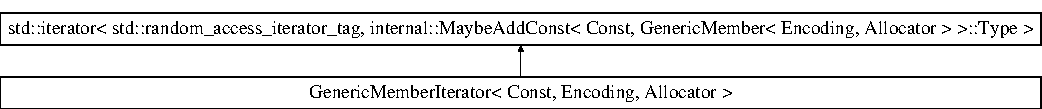
\includegraphics[height=1.462141cm]{classGenericMemberIterator}
\end{center}
\end{figure}
\subsection*{Public Types}
\begin{DoxyCompactItemize}
\item 
typedef \hyperlink{classGenericMemberIterator}{Generic\+Member\+Iterator} \hyperlink{classGenericMemberIterator_ad1cf1ecf6210b47906c9f179c893a8b8}{Iterator}\hypertarget{classGenericMemberIterator_ad1cf1ecf6210b47906c9f179c893a8b8}{}\label{classGenericMemberIterator_ad1cf1ecf6210b47906c9f179c893a8b8}

\begin{DoxyCompactList}\small\item\em Iterator type itself. \end{DoxyCompactList}\item 
typedef \hyperlink{classGenericMemberIterator}{Generic\+Member\+Iterator}$<$ true, Encoding, Allocator $>$ \hyperlink{classGenericMemberIterator_ae5be27a73dce0be58ee2776db896d591}{Const\+Iterator}\hypertarget{classGenericMemberIterator_ae5be27a73dce0be58ee2776db896d591}{}\label{classGenericMemberIterator_ae5be27a73dce0be58ee2776db896d591}

\begin{DoxyCompactList}\small\item\em Constant iterator type. \end{DoxyCompactList}\item 
typedef \hyperlink{classGenericMemberIterator}{Generic\+Member\+Iterator}$<$ false, Encoding, Allocator $>$ \hyperlink{classGenericMemberIterator_abc26eb06f2962765b11dcd06ce84ac02}{Non\+Const\+Iterator}\hypertarget{classGenericMemberIterator_abc26eb06f2962765b11dcd06ce84ac02}{}\label{classGenericMemberIterator_abc26eb06f2962765b11dcd06ce84ac02}

\begin{DoxyCompactList}\small\item\em Non-\/constant iterator type. \end{DoxyCompactList}\item 
typedef Base\+Type\+::pointer \hyperlink{classGenericMemberIterator_ac69f141f1fde31c1f550f524a69c5de9}{Pointer}\hypertarget{classGenericMemberIterator_ac69f141f1fde31c1f550f524a69c5de9}{}\label{classGenericMemberIterator_ac69f141f1fde31c1f550f524a69c5de9}

\begin{DoxyCompactList}\small\item\em Pointer to (const) \hyperlink{structGenericMember}{Generic\+Member}. \end{DoxyCompactList}\item 
typedef Base\+Type\+::reference \hyperlink{classGenericMemberIterator_ae80f6b601eb9e24f73aa75fb32b35c65}{Reference}\hypertarget{classGenericMemberIterator_ae80f6b601eb9e24f73aa75fb32b35c65}{}\label{classGenericMemberIterator_ae80f6b601eb9e24f73aa75fb32b35c65}

\begin{DoxyCompactList}\small\item\em Reference to (const) \hyperlink{structGenericMember}{Generic\+Member}. \end{DoxyCompactList}\item 
typedef Base\+Type\+::difference\+\_\+type \hyperlink{classGenericMemberIterator_a902b99c8ae351cd7626514dc5f30740a}{Difference\+Type}\hypertarget{classGenericMemberIterator_a902b99c8ae351cd7626514dc5f30740a}{}\label{classGenericMemberIterator_a902b99c8ae351cd7626514dc5f30740a}

\begin{DoxyCompactList}\small\item\em Signed integer type (e.\+g. {\ttfamily ptrdiff\+\_\+t}) \end{DoxyCompactList}\end{DoxyCompactItemize}
\subsection*{Public Member Functions}
\begin{DoxyCompactItemize}
\item 
\hyperlink{classGenericMemberIterator_a2708717d497a0aadacdf75900de4c5b4}{Generic\+Member\+Iterator} ()
\begin{DoxyCompactList}\small\item\em Default constructor (singular value) \end{DoxyCompactList}\item 
\hyperlink{classGenericMemberIterator_a2697fd327a90654b0bf91c988e43f95e}{Generic\+Member\+Iterator} (const \hyperlink{classGenericMemberIterator_abc26eb06f2962765b11dcd06ce84ac02}{Non\+Const\+Iterator} \&it)
\begin{DoxyCompactList}\small\item\em Iterator conversions to more const. \end{DoxyCompactList}\item 
\hyperlink{classGenericMemberIterator_ad1cf1ecf6210b47906c9f179c893a8b8}{Iterator} \& {\bfseries operator=} (const \hyperlink{classGenericMemberIterator_abc26eb06f2962765b11dcd06ce84ac02}{Non\+Const\+Iterator} \&it)\hypertarget{classGenericMemberIterator_a4ebb2b80e7d70c11802520ae77958df3}{}\label{classGenericMemberIterator_a4ebb2b80e7d70c11802520ae77958df3}

\item 
\hyperlink{classGenericMemberIterator_a902b99c8ae351cd7626514dc5f30740a}{Difference\+Type} \hyperlink{classGenericMemberIterator_a056851821e75c4be13b297604bc37c0b}{operator-\/} (\hyperlink{classGenericMemberIterator_ae5be27a73dce0be58ee2776db896d591}{Const\+Iterator} that) const \hypertarget{classGenericMemberIterator_a056851821e75c4be13b297604bc37c0b}{}\label{classGenericMemberIterator_a056851821e75c4be13b297604bc37c0b}

\begin{DoxyCompactList}\small\item\em Distance. \end{DoxyCompactList}\end{DoxyCompactItemize}
\begin{Indent}{\bf stepping}\par
\begin{DoxyCompactItemize}
\item 
\hyperlink{classGenericMemberIterator_ad1cf1ecf6210b47906c9f179c893a8b8}{Iterator} \& {\bfseries operator++} ()\hypertarget{classGenericMemberIterator_afd6c9a104e2285d1d0b50bde53c9109e}{}\label{classGenericMemberIterator_afd6c9a104e2285d1d0b50bde53c9109e}

\item 
\hyperlink{classGenericMemberIterator_ad1cf1ecf6210b47906c9f179c893a8b8}{Iterator} \& {\bfseries operator-\/-\/} ()\hypertarget{classGenericMemberIterator_a6db8972f02d74b663b6ef90ee3ff34f6}{}\label{classGenericMemberIterator_a6db8972f02d74b663b6ef90ee3ff34f6}

\item 
\hyperlink{classGenericMemberIterator_ad1cf1ecf6210b47906c9f179c893a8b8}{Iterator} {\bfseries operator++} (int)\hypertarget{classGenericMemberIterator_a83c8be6d960213ce32d68a880a8d9089}{}\label{classGenericMemberIterator_a83c8be6d960213ce32d68a880a8d9089}

\item 
\hyperlink{classGenericMemberIterator_ad1cf1ecf6210b47906c9f179c893a8b8}{Iterator} {\bfseries operator-\/-\/} (int)\hypertarget{classGenericMemberIterator_a4606c8baec5ea2b5139a503f7caa5444}{}\label{classGenericMemberIterator_a4606c8baec5ea2b5139a503f7caa5444}

\end{DoxyCompactItemize}
\end{Indent}
\begin{Indent}{\bf increment/decrement}\par
\begin{DoxyCompactItemize}
\item 
\hyperlink{classGenericMemberIterator_ad1cf1ecf6210b47906c9f179c893a8b8}{Iterator} {\bfseries operator+} (\hyperlink{classGenericMemberIterator_a902b99c8ae351cd7626514dc5f30740a}{Difference\+Type} n) const \hypertarget{classGenericMemberIterator_ac533ee1f689563a7276c3ace44dfe4e0}{}\label{classGenericMemberIterator_ac533ee1f689563a7276c3ace44dfe4e0}

\item 
\hyperlink{classGenericMemberIterator_ad1cf1ecf6210b47906c9f179c893a8b8}{Iterator} {\bfseries operator-\/} (\hyperlink{classGenericMemberIterator_a902b99c8ae351cd7626514dc5f30740a}{Difference\+Type} n) const \hypertarget{classGenericMemberIterator_a0152d4ec06c14f50279aa108a97216a7}{}\label{classGenericMemberIterator_a0152d4ec06c14f50279aa108a97216a7}

\item 
\hyperlink{classGenericMemberIterator_ad1cf1ecf6210b47906c9f179c893a8b8}{Iterator} \& {\bfseries operator+=} (\hyperlink{classGenericMemberIterator_a902b99c8ae351cd7626514dc5f30740a}{Difference\+Type} n)\hypertarget{classGenericMemberIterator_a1fc75f09d68b0f5d92f18ae8c4133e6a}{}\label{classGenericMemberIterator_a1fc75f09d68b0f5d92f18ae8c4133e6a}

\item 
\hyperlink{classGenericMemberIterator_ad1cf1ecf6210b47906c9f179c893a8b8}{Iterator} \& {\bfseries operator-\/=} (\hyperlink{classGenericMemberIterator_a902b99c8ae351cd7626514dc5f30740a}{Difference\+Type} n)\hypertarget{classGenericMemberIterator_a7cd0c5f194007ec24fa9fa5c13e2502a}{}\label{classGenericMemberIterator_a7cd0c5f194007ec24fa9fa5c13e2502a}

\end{DoxyCompactItemize}
\end{Indent}
\begin{Indent}{\bf relations}\par
\begin{DoxyCompactItemize}
\item 
bool {\bfseries operator==} (\hyperlink{classGenericMemberIterator_ae5be27a73dce0be58ee2776db896d591}{Const\+Iterator} that) const \hypertarget{classGenericMemberIterator_aacbaf8c5dfded8148a5ecd400338d457}{}\label{classGenericMemberIterator_aacbaf8c5dfded8148a5ecd400338d457}

\item 
bool {\bfseries operator!=} (\hyperlink{classGenericMemberIterator_ae5be27a73dce0be58ee2776db896d591}{Const\+Iterator} that) const \hypertarget{classGenericMemberIterator_a829ba40cafa98fd5ced56a07658ce0b7}{}\label{classGenericMemberIterator_a829ba40cafa98fd5ced56a07658ce0b7}

\item 
bool {\bfseries operator$<$=} (\hyperlink{classGenericMemberIterator_ae5be27a73dce0be58ee2776db896d591}{Const\+Iterator} that) const \hypertarget{classGenericMemberIterator_a395f81480589f78cb2497509730e36c3}{}\label{classGenericMemberIterator_a395f81480589f78cb2497509730e36c3}

\item 
bool {\bfseries operator$>$=} (\hyperlink{classGenericMemberIterator_ae5be27a73dce0be58ee2776db896d591}{Const\+Iterator} that) const \hypertarget{classGenericMemberIterator_afe815c6a0cd2f72f800b59fdb443d223}{}\label{classGenericMemberIterator_afe815c6a0cd2f72f800b59fdb443d223}

\item 
bool {\bfseries operator$<$} (\hyperlink{classGenericMemberIterator_ae5be27a73dce0be58ee2776db896d591}{Const\+Iterator} that) const \hypertarget{classGenericMemberIterator_a6a897b2e89822d798c985008fc3a9a18}{}\label{classGenericMemberIterator_a6a897b2e89822d798c985008fc3a9a18}

\item 
bool {\bfseries operator$>$} (\hyperlink{classGenericMemberIterator_ae5be27a73dce0be58ee2776db896d591}{Const\+Iterator} that) const \hypertarget{classGenericMemberIterator_a89c57197cd49cfa6cf98e3bdf1454640}{}\label{classGenericMemberIterator_a89c57197cd49cfa6cf98e3bdf1454640}

\end{DoxyCompactItemize}
\end{Indent}
\begin{Indent}{\bf dereference}\par
\begin{DoxyCompactItemize}
\item 
\hyperlink{classGenericMemberIterator_ae80f6b601eb9e24f73aa75fb32b35c65}{Reference} {\bfseries operator$\ast$} () const \hypertarget{classGenericMemberIterator_a37f5cb3b669682da70fe3e5ec6bc4775}{}\label{classGenericMemberIterator_a37f5cb3b669682da70fe3e5ec6bc4775}

\item 
\hyperlink{classGenericMemberIterator_ac69f141f1fde31c1f550f524a69c5de9}{Pointer} {\bfseries operator-\/$>$} () const \hypertarget{classGenericMemberIterator_a2e3d0e0f9a5c0ca69f09e4927ed985c3}{}\label{classGenericMemberIterator_a2e3d0e0f9a5c0ca69f09e4927ed985c3}

\item 
\hyperlink{classGenericMemberIterator_ae80f6b601eb9e24f73aa75fb32b35c65}{Reference} {\bfseries operator\mbox{[}$\,$\mbox{]}} (\hyperlink{classGenericMemberIterator_a902b99c8ae351cd7626514dc5f30740a}{Difference\+Type} n) const \hypertarget{classGenericMemberIterator_ae83095869e033554257e3f33df59fcfb}{}\label{classGenericMemberIterator_ae83095869e033554257e3f33df59fcfb}

\end{DoxyCompactItemize}
\end{Indent}
\subsection*{Friends}
\begin{DoxyCompactItemize}
\item 
class {\bfseries Generic\+Value$<$ Encoding, Allocator $>$}\hypertarget{classGenericMemberIterator_a82bdd5798f1a5ac0e3e7ba4bd6938cfc}{}\label{classGenericMemberIterator_a82bdd5798f1a5ac0e3e7ba4bd6938cfc}

\item 
{\footnotesize template$<$bool , typename , typename $>$ }\\class {\bfseries Generic\+Member\+Iterator}\hypertarget{classGenericMemberIterator_aa375aeb1ffac85cddc3a72a6c24ec6e1}{}\label{classGenericMemberIterator_aa375aeb1ffac85cddc3a72a6c24ec6e1}

\end{DoxyCompactItemize}


\subsection{Detailed Description}
\subsubsection*{template$<$bool Const, typename Encoding, typename Allocator$>$\\*
class Generic\+Member\+Iterator$<$ Const, Encoding, Allocator $>$}

(Constant) member iterator for a J\+S\+ON object value 


\begin{DoxyTemplParams}{Template Parameters}
{\em Const} & Is this a constant iterator? \\
\hline
{\em Encoding} & Encoding of the value. (Even non-\/string values need to have the same encoding in a document) \\
\hline
{\em Allocator} & Allocator type for allocating memory of object, array and string.\\
\hline
\end{DoxyTemplParams}
This class implements a Random Access Iterator for \hyperlink{structGenericMember}{Generic\+Member} elements of a \hyperlink{classGenericValue}{Generic\+Value}, see I\+S\+O/\+I\+EC 14882\+:2003(E) C++ standard, 24.\+1 \mbox{[}lib.\+iterator.\+requirements\mbox{]}.

\begin{DoxyNote}{Note}
This iterator implementation is mainly intended to avoid implicit conversions from iterator values to {\ttfamily N\+U\+LL}, e.\+g. from Generic\+Value\+::\+Find\+Member.

Define {\ttfamily R\+A\+P\+I\+D\+J\+S\+O\+N\+\_\+\+N\+O\+M\+E\+M\+B\+E\+R\+I\+T\+E\+R\+A\+T\+O\+R\+C\+L\+A\+SS} to fall back to a pointer-\/based implementation, if your platform doesn\textquotesingle{}t provide the C++ $<$iterator$>$ header.
\end{DoxyNote}
\begin{DoxySeeAlso}{See also}
\hyperlink{structGenericMember}{Generic\+Member}, \hyperlink{classGenericValue_a349b8faae61edc42b4289726820be439}{Generic\+Value\+::\+Member\+Iterator}, \hyperlink{classGenericValue_aac08c3e660a9036d3dcb8b10ff6c61f4}{Generic\+Value\+::\+Const\+Member\+Iterator} 
\end{DoxySeeAlso}


\subsection{Constructor \& Destructor Documentation}
\index{Generic\+Member\+Iterator@{Generic\+Member\+Iterator}!Generic\+Member\+Iterator@{Generic\+Member\+Iterator}}
\index{Generic\+Member\+Iterator@{Generic\+Member\+Iterator}!Generic\+Member\+Iterator@{Generic\+Member\+Iterator}}
\subsubsection[{\texorpdfstring{Generic\+Member\+Iterator()}{GenericMemberIterator()}}]{\setlength{\rightskip}{0pt plus 5cm}template$<$bool Const, typename Encoding , typename Allocator $>$ {\bf Generic\+Member\+Iterator}$<$ Const, Encoding, Allocator $>$\+::{\bf Generic\+Member\+Iterator} (
\begin{DoxyParamCaption}
{}
\end{DoxyParamCaption}
)\hspace{0.3cm}{\ttfamily [inline]}}\hypertarget{classGenericMemberIterator_a2708717d497a0aadacdf75900de4c5b4}{}\label{classGenericMemberIterator_a2708717d497a0aadacdf75900de4c5b4}


Default constructor (singular value) 

Creates an iterator pointing to no element. \begin{DoxyNote}{Note}
All operations, except for comparisons, are undefined on such values. 
\end{DoxyNote}
\index{Generic\+Member\+Iterator@{Generic\+Member\+Iterator}!Generic\+Member\+Iterator@{Generic\+Member\+Iterator}}
\index{Generic\+Member\+Iterator@{Generic\+Member\+Iterator}!Generic\+Member\+Iterator@{Generic\+Member\+Iterator}}
\subsubsection[{\texorpdfstring{Generic\+Member\+Iterator(const Non\+Const\+Iterator \&it)}{GenericMemberIterator(const NonConstIterator &it)}}]{\setlength{\rightskip}{0pt plus 5cm}template$<$bool Const, typename Encoding , typename Allocator $>$ {\bf Generic\+Member\+Iterator}$<$ Const, Encoding, Allocator $>$\+::{\bf Generic\+Member\+Iterator} (
\begin{DoxyParamCaption}
\item[{const {\bf Non\+Const\+Iterator} \&}]{it}
\end{DoxyParamCaption}
)\hspace{0.3cm}{\ttfamily [inline]}}\hypertarget{classGenericMemberIterator_a2697fd327a90654b0bf91c988e43f95e}{}\label{classGenericMemberIterator_a2697fd327a90654b0bf91c988e43f95e}


Iterator conversions to more const. 


\begin{DoxyParams}{Parameters}
{\em it} & (Non-\/const) iterator to copy from\\
\hline
\end{DoxyParams}
Allows the creation of an iterator from another \hyperlink{classGenericMemberIterator}{Generic\+Member\+Iterator} that is \char`\"{}less const\char`\"{}. Especially, creating a non-\/constant iterator from a constant iterator are disabled\+: \begin{DoxyItemize}
\item const -\/$>$ non-\/const (not ok) \item const -\/$>$ const (ok) \item non-\/const -\/$>$ const (ok) \item non-\/const -\/$>$ non-\/const (ok)\end{DoxyItemize}
\begin{DoxyNote}{Note}
If the {\ttfamily Const} template parameter is already {\ttfamily false}, this constructor effectively defines a regular copy-\/constructor. Otherwise, the copy constructor is implicitly defined. 
\end{DoxyNote}


The documentation for this class was generated from the following file\+:\begin{DoxyCompactItemize}
\item 
/home/mate/\+Documents/\+Programming/\+Research/\+Multilayer\+Network\+Model/\+Multilayer\+Network\+Model/src/external/rapidjson/\hyperlink{document_8h}{document.\+h}\end{DoxyCompactItemize}

\hypertarget{structGenericMemoryBuffer}{}\section{Generic\+Memory\+Buffer$<$ Allocator $>$ Struct Template Reference}
\label{structGenericMemoryBuffer}\index{Generic\+Memory\+Buffer$<$ Allocator $>$@{Generic\+Memory\+Buffer$<$ Allocator $>$}}


Represents an in-\/memory output byte stream.  




{\ttfamily \#include $<$memorybuffer.\+h$>$}

\subsection*{Public Types}
\begin{DoxyCompactItemize}
\item 
typedef char {\bfseries Ch}\hypertarget{structGenericMemoryBuffer_a212f137abfd8bce2ad216b2d960c027f}{}\label{structGenericMemoryBuffer_a212f137abfd8bce2ad216b2d960c027f}

\end{DoxyCompactItemize}
\subsection*{Public Member Functions}
\begin{DoxyCompactItemize}
\item 
{\bfseries Generic\+Memory\+Buffer} (Allocator $\ast$allocator=0, size\+\_\+t capacity=k\+Default\+Capacity)\hypertarget{structGenericMemoryBuffer_ad08f7da47bca43fcdb0c3b10e22dfa1d}{}\label{structGenericMemoryBuffer_ad08f7da47bca43fcdb0c3b10e22dfa1d}

\item 
void {\bfseries Put} (Ch c)\hypertarget{structGenericMemoryBuffer_a9dfb477983e211893601f8ab637b42d8}{}\label{structGenericMemoryBuffer_a9dfb477983e211893601f8ab637b42d8}

\item 
void {\bfseries Flush} ()\hypertarget{structGenericMemoryBuffer_a9861181cab6f5bec2ec08b601aa53575}{}\label{structGenericMemoryBuffer_a9861181cab6f5bec2ec08b601aa53575}

\item 
void {\bfseries Clear} ()\hypertarget{structGenericMemoryBuffer_a036cbe2556778e1edc525602a9821df2}{}\label{structGenericMemoryBuffer_a036cbe2556778e1edc525602a9821df2}

\item 
void {\bfseries Shrink\+To\+Fit} ()\hypertarget{structGenericMemoryBuffer_a3b87deb9bf34c394c8fb262ab53c0c4b}{}\label{structGenericMemoryBuffer_a3b87deb9bf34c394c8fb262ab53c0c4b}

\item 
Ch $\ast$ {\bfseries Push} (size\+\_\+t count)\hypertarget{structGenericMemoryBuffer_a56f7b14d2940b682fe592f598d6792ec}{}\label{structGenericMemoryBuffer_a56f7b14d2940b682fe592f598d6792ec}

\item 
void {\bfseries Pop} (size\+\_\+t count)\hypertarget{structGenericMemoryBuffer_a82a6706286f1356e1769282f5d496005}{}\label{structGenericMemoryBuffer_a82a6706286f1356e1769282f5d496005}

\item 
const Ch $\ast$ {\bfseries Get\+Buffer} () const \hypertarget{structGenericMemoryBuffer_a9afc78eef159fcbc10d0cea84ccfb26d}{}\label{structGenericMemoryBuffer_a9afc78eef159fcbc10d0cea84ccfb26d}

\item 
size\+\_\+t {\bfseries Get\+Size} () const \hypertarget{structGenericMemoryBuffer_adc22f10318fa6dbdf7eb1fa9041bb68d}{}\label{structGenericMemoryBuffer_adc22f10318fa6dbdf7eb1fa9041bb68d}

\end{DoxyCompactItemize}
\subsection*{Public Attributes}
\begin{DoxyCompactItemize}
\item 
\hyperlink{classinternal_1_1Stack}{internal\+::\+Stack}$<$ Allocator $>$ {\bfseries stack\+\_\+}\hypertarget{structGenericMemoryBuffer_a977b479180bebe8ae14ca1c11d52a486}{}\label{structGenericMemoryBuffer_a977b479180bebe8ae14ca1c11d52a486}

\end{DoxyCompactItemize}
\subsection*{Static Public Attributes}
\begin{DoxyCompactItemize}
\item 
static const size\+\_\+t {\bfseries k\+Default\+Capacity} = 256\hypertarget{structGenericMemoryBuffer_af6ecdbdbb8d3aa53cdef6e788e4980be}{}\label{structGenericMemoryBuffer_af6ecdbdbb8d3aa53cdef6e788e4980be}

\end{DoxyCompactItemize}


\subsection{Detailed Description}
\subsubsection*{template$<$typename Allocator = Crt\+Allocator$>$\\*
struct Generic\+Memory\+Buffer$<$ Allocator $>$}

Represents an in-\/memory output byte stream. 

This class is mainly for being wrapped by \hyperlink{classEncodedOutputStream}{Encoded\+Output\+Stream} or \hyperlink{classAutoUTFOutputStream}{Auto\+U\+T\+F\+Output\+Stream}.

It is similar to File\+Write\+Buffer but the destination is an in-\/memory buffer instead of a file.

Differences between Memory\+Buffer and String\+Buffer\+:
\begin{DoxyEnumerate}
\item String\+Buffer has Encoding but Memory\+Buffer is only a byte buffer.
\item String\+Buffer\+::\+Get\+String() returns a null-\/terminated string. Memory\+Buffer\+::\+Get\+Buffer() returns a buffer without terminator.
\end{DoxyEnumerate}


\begin{DoxyTemplParams}{Template Parameters}
{\em Allocator} & type for allocating memory buffer. \\
\hline
\end{DoxyTemplParams}
\begin{DoxyNote}{Note}
implements Stream concept 
\end{DoxyNote}


The documentation for this struct was generated from the following files\+:\begin{DoxyCompactItemize}
\item 
/home/mate/\+Documents/\+Programming/\+Research/\+Multilayer\+Network\+Model/\+Multilayer\+Network\+Model/sources/external/rapidjson/fwd.\+h\item 
/home/mate/\+Documents/\+Programming/\+Research/\+Multilayer\+Network\+Model/\+Multilayer\+Network\+Model/sources/external/rapidjson/memorybuffer.\+h\end{DoxyCompactItemize}

\hypertarget{classGenericObject}{}\section{Generic\+Object$<$ Const, ValueT $>$ Class Template Reference}
\label{classGenericObject}\index{Generic\+Object$<$ Const, Value\+T $>$@{Generic\+Object$<$ Const, Value\+T $>$}}


Helper class for accessing Value of object type.  




{\ttfamily \#include $<$document.\+h$>$}

\subsection*{Public Types}
\begin{DoxyCompactItemize}
\item 
typedef \hyperlink{classGenericObject}{Generic\+Object}$<$ true, ValueT $>$ {\bfseries Const\+Object}\hypertarget{classGenericObject_aeee588f9a85e88cac89b7c4dfb6b0bd3}{}\label{classGenericObject_aeee588f9a85e88cac89b7c4dfb6b0bd3}

\item 
typedef \hyperlink{classGenericObject}{Generic\+Object}$<$ false, ValueT $>$ {\bfseries Object}\hypertarget{classGenericObject_ae8f5673d0cf8e7ebfd2d4f6ab27b632d}{}\label{classGenericObject_ae8f5673d0cf8e7ebfd2d4f6ab27b632d}

\item 
typedef ValueT {\bfseries Plain\+Type}\hypertarget{classGenericObject_a4c25f4a5f696745c418b91ad9f577f12}{}\label{classGenericObject_a4c25f4a5f696745c418b91ad9f577f12}

\item 
typedef internal\+::\+Maybe\+Add\+Const$<$ Const, Plain\+Type $>$\+::\hyperlink{rapidjson_8h_a1d1cfd8ffb84e947f82999c682b666a7}{Type} {\bfseries Value\+Type}\hypertarget{classGenericObject_a930aa30f89caee7ba7bff60bf9dc21b1}{}\label{classGenericObject_a930aa30f89caee7ba7bff60bf9dc21b1}

\item 
typedef \hyperlink{classGenericMemberIterator}{Generic\+Member\+Iterator}$<$ Const, typename Value\+T\+::\+Encoding\+Type, typename Value\+T\+::\+Allocator\+Type $>$ {\bfseries Member\+Iterator}\hypertarget{classGenericObject_a1f531d70f8d57ed30199ac445b5935e6}{}\label{classGenericObject_a1f531d70f8d57ed30199ac445b5935e6}

\item 
typedef \hyperlink{classGenericMemberIterator}{Generic\+Member\+Iterator}$<$ true, typename Value\+T\+::\+Encoding\+Type, typename Value\+T\+::\+Allocator\+Type $>$ {\bfseries Const\+Member\+Iterator}\hypertarget{classGenericObject_af16706c0ad32b957c56e7d0541628cd5}{}\label{classGenericObject_af16706c0ad32b957c56e7d0541628cd5}

\item 
typedef Value\+Type\+::\+Allocator\+Type {\bfseries Allocator\+Type}\hypertarget{classGenericObject_a00c8cee952d5ebadc5e1c309aa489ad9}{}\label{classGenericObject_a00c8cee952d5ebadc5e1c309aa489ad9}

\item 
typedef Value\+Type\+::\+String\+Ref\+Type {\bfseries String\+Ref\+Type}\hypertarget{classGenericObject_a9b8381fc96f5f89b2163b052ed66cc59}{}\label{classGenericObject_a9b8381fc96f5f89b2163b052ed66cc59}

\item 
typedef Value\+Type\+::\+Encoding\+Type {\bfseries Encoding\+Type}\hypertarget{classGenericObject_a96ebfdde095e2ce42535d15ae5dc58ef}{}\label{classGenericObject_a96ebfdde095e2ce42535d15ae5dc58ef}

\item 
typedef Value\+Type\+::\+Ch {\bfseries Ch}\hypertarget{classGenericObject_ac6747e5baa13e15bcea1658b5624647a}{}\label{classGenericObject_ac6747e5baa13e15bcea1658b5624647a}

\end{DoxyCompactItemize}
\subsection*{Public Member Functions}
\begin{DoxyCompactItemize}
\item 
{\bfseries Generic\+Object} (const \hyperlink{classGenericObject}{Generic\+Object} \&rhs)\hypertarget{classGenericObject_a10173c42d0e8a71ca0e3ae75d800887a}{}\label{classGenericObject_a10173c42d0e8a71ca0e3ae75d800887a}

\item 
\hyperlink{classGenericObject}{Generic\+Object} \& {\bfseries operator=} (const \hyperlink{classGenericObject}{Generic\+Object} \&rhs)\hypertarget{classGenericObject_af8984f76d6f3b13039c6d3b8e217f747}{}\label{classGenericObject_af8984f76d6f3b13039c6d3b8e217f747}

\item 
\hyperlink{rapidjson_8h_a5ed6e6e67250fadbd041127e6386dcb5}{Size\+Type} {\bfseries Member\+Count} () const \hypertarget{classGenericObject_ab3772740b811ed417924cebdace1d190}{}\label{classGenericObject_ab3772740b811ed417924cebdace1d190}

\item 
\hyperlink{rapidjson_8h_a5ed6e6e67250fadbd041127e6386dcb5}{Size\+Type} {\bfseries Member\+Capacity} () const \hypertarget{classGenericObject_a3aea2ee68b9ff649fee0b9a8c375a34a}{}\label{classGenericObject_a3aea2ee68b9ff649fee0b9a8c375a34a}

\item 
bool {\bfseries Object\+Empty} () const \hypertarget{classGenericObject_a410e5dfd7fa047852ecb4b719a74f842}{}\label{classGenericObject_a410e5dfd7fa047852ecb4b719a74f842}

\item 
{\footnotesize template$<$typename T $>$ }\\Value\+Type \& {\bfseries operator\mbox{[}$\,$\mbox{]}} (T $\ast$name) const \hypertarget{classGenericObject_af3db47f1615353d0c5ce974c2fbe7885}{}\label{classGenericObject_af3db47f1615353d0c5ce974c2fbe7885}

\item 
{\footnotesize template$<$typename Source\+Allocator $>$ }\\Value\+Type \& {\bfseries operator\mbox{[}$\,$\mbox{]}} (const \hyperlink{classGenericValue}{Generic\+Value}$<$ Encoding\+Type, Source\+Allocator $>$ \&name) const \hypertarget{classGenericObject_aac0937f20bfdc94380641bb02cefbf98}{}\label{classGenericObject_aac0937f20bfdc94380641bb02cefbf98}

\item 
\hyperlink{classGenericMemberIterator}{Member\+Iterator} {\bfseries Member\+Begin} () const \hypertarget{classGenericObject_abf56b2ac9cface0dffd21b541acb9511}{}\label{classGenericObject_abf56b2ac9cface0dffd21b541acb9511}

\item 
\hyperlink{classGenericMemberIterator}{Member\+Iterator} {\bfseries Member\+End} () const \hypertarget{classGenericObject_a7dedae79a478db0aeb4e01df4c788f3a}{}\label{classGenericObject_a7dedae79a478db0aeb4e01df4c788f3a}

\item 
\hyperlink{classGenericObject}{Generic\+Object} {\bfseries Member\+Reserve} (\hyperlink{rapidjson_8h_a5ed6e6e67250fadbd041127e6386dcb5}{Size\+Type} new\+Capacity, Allocator\+Type \&allocator) const \hypertarget{classGenericObject_ae3b031d6df53942eb8909ed914641e00}{}\label{classGenericObject_ae3b031d6df53942eb8909ed914641e00}

\item 
bool {\bfseries Has\+Member} (const Ch $\ast$name) const \hypertarget{classGenericObject_a545cbb3d1e99a48fd7a40ebeac1d10da}{}\label{classGenericObject_a545cbb3d1e99a48fd7a40ebeac1d10da}

\item 
{\footnotesize template$<$typename Source\+Allocator $>$ }\\bool {\bfseries Has\+Member} (const \hyperlink{classGenericValue}{Generic\+Value}$<$ Encoding\+Type, Source\+Allocator $>$ \&name) const \hypertarget{classGenericObject_a946712fa1b4fc9ab551a63d17d671f47}{}\label{classGenericObject_a946712fa1b4fc9ab551a63d17d671f47}

\item 
\hyperlink{classGenericMemberIterator}{Member\+Iterator} {\bfseries Find\+Member} (const Ch $\ast$name) const \hypertarget{classGenericObject_a6713425c66b7f05e4ac5d251a8f5b708}{}\label{classGenericObject_a6713425c66b7f05e4ac5d251a8f5b708}

\item 
{\footnotesize template$<$typename Source\+Allocator $>$ }\\\hyperlink{classGenericMemberIterator}{Member\+Iterator} {\bfseries Find\+Member} (const \hyperlink{classGenericValue}{Generic\+Value}$<$ Encoding\+Type, Source\+Allocator $>$ \&name) const \hypertarget{classGenericObject_a3eca7c61d4d2b728de83ffdb1f35e45a}{}\label{classGenericObject_a3eca7c61d4d2b728de83ffdb1f35e45a}

\item 
\hyperlink{classGenericObject}{Generic\+Object} {\bfseries Add\+Member} (Value\+Type \&name, Value\+Type \&value, Allocator\+Type \&allocator) const \hypertarget{classGenericObject_a59554f8232c7c2a74d8043f4b4b20ec2}{}\label{classGenericObject_a59554f8232c7c2a74d8043f4b4b20ec2}

\item 
\hyperlink{classGenericObject}{Generic\+Object} {\bfseries Add\+Member} (Value\+Type \&name, String\+Ref\+Type value, Allocator\+Type \&allocator) const \hypertarget{classGenericObject_a33df672a1ecafa47c2d7ed3c765738c1}{}\label{classGenericObject_a33df672a1ecafa47c2d7ed3c765738c1}

\item 
{\footnotesize template$<$typename T $>$ }\\{\bfseries R\+A\+P\+I\+D\+J\+S\+O\+N\+\_\+\+D\+I\+S\+A\+B\+L\+E\+I\+F\+\_\+\+R\+E\+T\+U\+RN} ((internal\+::\+Or\+Expr$<$ internal\+::\+Is\+Pointer$<$ T $>$, \hyperlink{structinternal_1_1IsGenericValue}{internal\+::\+Is\+Generic\+Value}$<$ T $>$ $>$),(Value\+Type \&)) Add\+Member(Value\+Type \&name\hypertarget{classGenericObject_a98ebcec632c41442d89cd8634b7ecc47}{}\label{classGenericObject_a98ebcec632c41442d89cd8634b7ecc47}

\item 
\hyperlink{classGenericObject}{Generic\+Object} {\bfseries Add\+Member} (String\+Ref\+Type name, Value\+Type \&value, Allocator\+Type \&allocator) const \hypertarget{classGenericObject_a245647b72d87ffe6142d1c656f0e92d8}{}\label{classGenericObject_a245647b72d87ffe6142d1c656f0e92d8}

\item 
\hyperlink{classGenericObject}{Generic\+Object} {\bfseries Add\+Member} (String\+Ref\+Type name, String\+Ref\+Type value, Allocator\+Type \&allocator) const \hypertarget{classGenericObject_a5cb6c166992abe5674a287bbc02d8f2f}{}\label{classGenericObject_a5cb6c166992abe5674a287bbc02d8f2f}

\item 
{\footnotesize template$<$typename T $>$ }\\{\bfseries R\+A\+P\+I\+D\+J\+S\+O\+N\+\_\+\+D\+I\+S\+A\+B\+L\+E\+I\+F\+\_\+\+R\+E\+T\+U\+RN} ((internal\+::\+Or\+Expr$<$ internal\+::\+Is\+Pointer$<$ T $>$, \hyperlink{structinternal_1_1IsGenericValue}{internal\+::\+Is\+Generic\+Value}$<$ T $>$ $>$),(\hyperlink{classGenericObject}{Generic\+Object})) Add\+Member(String\+Ref\+Type name\hypertarget{classGenericObject_af361a4b677882964789201fc605541d0}{}\label{classGenericObject_af361a4b677882964789201fc605541d0}

\item 
void {\bfseries Remove\+All\+Members} ()\hypertarget{classGenericObject_a129ce3843a6658e620a7f740d9f44ee1}{}\label{classGenericObject_a129ce3843a6658e620a7f740d9f44ee1}

\item 
bool {\bfseries Remove\+Member} (const Ch $\ast$name) const \hypertarget{classGenericObject_a64bfcf1671efa5de04cc7659a014a29d}{}\label{classGenericObject_a64bfcf1671efa5de04cc7659a014a29d}

\item 
{\footnotesize template$<$typename Source\+Allocator $>$ }\\bool {\bfseries Remove\+Member} (const \hyperlink{classGenericValue}{Generic\+Value}$<$ Encoding\+Type, Source\+Allocator $>$ \&name) const \hypertarget{classGenericObject_acca9953e3c2e6df16d7685572ac3fe9d}{}\label{classGenericObject_acca9953e3c2e6df16d7685572ac3fe9d}

\item 
\hyperlink{classGenericMemberIterator}{Member\+Iterator} {\bfseries Remove\+Member} (\hyperlink{classGenericMemberIterator}{Member\+Iterator} m) const \hypertarget{classGenericObject_a2489d8522f3c38324df69f6184cd639a}{}\label{classGenericObject_a2489d8522f3c38324df69f6184cd639a}

\item 
\hyperlink{classGenericMemberIterator}{Member\+Iterator} {\bfseries Erase\+Member} (\hyperlink{classGenericMemberIterator}{Const\+Member\+Iterator} pos) const \hypertarget{classGenericObject_a85ed6e1f586c775a02aaa99d0deabcb4}{}\label{classGenericObject_a85ed6e1f586c775a02aaa99d0deabcb4}

\item 
\hyperlink{classGenericMemberIterator}{Member\+Iterator} {\bfseries Erase\+Member} (\hyperlink{classGenericMemberIterator}{Const\+Member\+Iterator} first, \hyperlink{classGenericMemberIterator}{Const\+Member\+Iterator} last) const \hypertarget{classGenericObject_a04c3ce4a9076ab2f7e8f6c5031456c29}{}\label{classGenericObject_a04c3ce4a9076ab2f7e8f6c5031456c29}

\item 
bool {\bfseries Erase\+Member} (const Ch $\ast$name) const \hypertarget{classGenericObject_abcf63f10bbc634620e03bf8b375fa6fd}{}\label{classGenericObject_abcf63f10bbc634620e03bf8b375fa6fd}

\item 
{\footnotesize template$<$typename Source\+Allocator $>$ }\\bool {\bfseries Erase\+Member} (const \hyperlink{classGenericValue}{Generic\+Value}$<$ Encoding\+Type, Source\+Allocator $>$ \&name) const \hypertarget{classGenericObject_afda9d121d16de8b70f7bf09621851218}{}\label{classGenericObject_afda9d121d16de8b70f7bf09621851218}

\end{DoxyCompactItemize}
\subsection*{Public Attributes}
\begin{DoxyCompactItemize}
\item 
T {\bfseries value}\hypertarget{classGenericObject_a131538fbbacbc0a3a5ad15dbea66394f}{}\label{classGenericObject_a131538fbbacbc0a3a5ad15dbea66394f}

\item 
T Allocator\+Type \&allocator {\bfseries const} \{ value\+\_\+.\+Add\+Member(name, value, allocator)\hypertarget{classGenericObject_af70c9646b5e422306c33e98b3d8783a7}{}\label{classGenericObject_af70c9646b5e422306c33e98b3d8783a7}

\item 
return $\ast$ {\bfseries this}\hypertarget{classGenericObject_a719a0e5501da825e6f86ce12b46446cb}{}\label{classGenericObject_a719a0e5501da825e6f86ce12b46446cb}

\end{DoxyCompactItemize}
\subsection*{Friends}
\begin{DoxyCompactItemize}
\item 
{\footnotesize template$<$typename , typename $>$ }\\class {\bfseries Generic\+Value}\hypertarget{classGenericObject_a899449e1a645b5e377af059fb61113d8}{}\label{classGenericObject_a899449e1a645b5e377af059fb61113d8}

\end{DoxyCompactItemize}


\subsection{Detailed Description}
\subsubsection*{template$<$bool Const, typename ValueT$>$\\*
class Generic\+Object$<$ Const, Value\+T $>$}

Helper class for accessing Value of object type. 

Instance of this helper class is obtained by {\ttfamily Generic\+Value\+::\+Get\+Object()}. In addition to all A\+P\+Is for array type, it provides range-\/based for loop if {\ttfamily R\+A\+P\+I\+D\+J\+S\+O\+N\+\_\+\+H\+A\+S\+\_\+\+C\+X\+X11\+\_\+\+R\+A\+N\+G\+E\+\_\+\+F\+OR=1}. 

The documentation for this class was generated from the following file\+:\begin{DoxyCompactItemize}
\item 
/home/mate/\+Documents/\+Programming/\+Research/\+Multilayer\+Network\+Model/\+Multilayer\+Network\+Model/sources/external/rapidjson/\hyperlink{document_8h}{document.\+h}\end{DoxyCompactItemize}

\hypertarget{classGenericPointer}{}\section{Generic\+Pointer$<$ Value\+Type, Allocator $>$ Class Template Reference}
\label{classGenericPointer}\index{Generic\+Pointer$<$ Value\+Type, Allocator $>$@{Generic\+Pointer$<$ Value\+Type, Allocator $>$}}


Represents a J\+S\+ON Pointer. Use Pointer for \hyperlink{structUTF8}{U\+T\+F8} encoding and default allocator.  




{\ttfamily \#include $<$pointer.\+h$>$}

\subsection*{Classes}
\begin{DoxyCompactItemize}
\item 
struct \hyperlink{structGenericPointer_1_1Token}{Token}
\begin{DoxyCompactList}\small\item\em A token is the basic units of internal representation. \end{DoxyCompactList}\end{DoxyCompactItemize}
\subsection*{Public Types}
\begin{DoxyCompactItemize}
\item 
typedef Value\+Type\+::\+Encoding\+Type \hyperlink{classGenericPointer_a4b802da797a7a0b615fd9611cedb7c3b}{Encoding\+Type}\hypertarget{classGenericPointer_a4b802da797a7a0b615fd9611cedb7c3b}{}\label{classGenericPointer_a4b802da797a7a0b615fd9611cedb7c3b}

\begin{DoxyCompactList}\small\item\em Encoding type from Value. \end{DoxyCompactList}\item 
typedef Value\+Type\+::\+Ch \hyperlink{classGenericPointer_ab292356c11b4015c98d21b966b11f285}{Ch}\hypertarget{classGenericPointer_ab292356c11b4015c98d21b966b11f285}{}\label{classGenericPointer_ab292356c11b4015c98d21b966b11f285}

\begin{DoxyCompactList}\small\item\em Character type from Value. \end{DoxyCompactList}\end{DoxyCompactItemize}
\subsection*{Public Member Functions}
\begin{DoxyCompactItemize}
\item 
Allocator stack\+Allocator {\bfseries R\+A\+P\+I\+D\+J\+S\+O\+N\+\_\+\+D\+I\+S\+A\+B\+L\+E\+I\+F\+\_\+\+R\+E\+T\+U\+RN} ((internal\+::\+Or\+Expr$<$ internal\+::\+Is\+Pointer$<$ T $>$, \hyperlink{structinternal_1_1IsGenericValue}{internal\+::\+Is\+Generic\+Value}$<$ T $>$ $>$),(Value\+Type \&)) Get\+With\+Default(\hyperlink{classGenericDocument}{Generic\+Document}$<$ \hyperlink{classGenericPointer_a4b802da797a7a0b615fd9611cedb7c3b}{Encoding\+Type}\hypertarget{classGenericPointer_aebf325c6fde06adfc4d959b507d7f170}{}\label{classGenericPointer_aebf325c6fde06adfc4d959b507d7f170}

\item 
bool \hyperlink{classGenericPointer_aa8fd4b1259fc500188f4162571b280ec}{Erase} (Value\+Type \&root) const 
\begin{DoxyCompactList}\small\item\em Erase a value in a subtree. \end{DoxyCompactList}\end{DoxyCompactItemize}
\begin{Indent}{\bf Constructors and destructor.}\par
\begin{DoxyCompactItemize}
\item 
\hyperlink{classGenericPointer_a5d85b7dc82719643e8f7adccd5a74fbe}{Generic\+Pointer} (Allocator $\ast$allocator=0)\hypertarget{classGenericPointer_a5d85b7dc82719643e8f7adccd5a74fbe}{}\label{classGenericPointer_a5d85b7dc82719643e8f7adccd5a74fbe}

\begin{DoxyCompactList}\small\item\em Default constructor. \end{DoxyCompactList}\item 
\hyperlink{classGenericPointer_a4ad549b8a826c3c2dedf03fcc07be9b0}{Generic\+Pointer} (const \hyperlink{classGenericPointer_ab292356c11b4015c98d21b966b11f285}{Ch} $\ast$source, Allocator $\ast$allocator=0)
\begin{DoxyCompactList}\small\item\em Constructor that parses a string or U\+RI fragment representation. \end{DoxyCompactList}\item 
\hyperlink{classGenericPointer_a9c05684ea95306aac7626e70cb3946cc}{Generic\+Pointer} (const \hyperlink{classGenericPointer_ab292356c11b4015c98d21b966b11f285}{Ch} $\ast$source, size\+\_\+t length, Allocator $\ast$allocator=0)
\begin{DoxyCompactList}\small\item\em Constructor that parses a string or U\+RI fragment representation, with length of the source string. \end{DoxyCompactList}\item 
\hyperlink{classGenericPointer_a524a9921eff68f389a817a20ca7f1d84}{Generic\+Pointer} (const \hyperlink{structGenericPointer_1_1Token}{Token} $\ast$tokens, size\+\_\+t token\+Count)
\begin{DoxyCompactList}\small\item\em Constructor with user-\/supplied tokens. \end{DoxyCompactList}\item 
\hyperlink{classGenericPointer_a18d671bb793c6b843d5496b2b130cb70}{Generic\+Pointer} (const \hyperlink{classGenericPointer}{Generic\+Pointer} \&rhs, Allocator $\ast$allocator=0)\hypertarget{classGenericPointer_a18d671bb793c6b843d5496b2b130cb70}{}\label{classGenericPointer_a18d671bb793c6b843d5496b2b130cb70}

\begin{DoxyCompactList}\small\item\em Copy constructor. \end{DoxyCompactList}\item 
\hyperlink{classGenericPointer_acf3eb2f7c4ebf9256f638aafa17534cb}{$\sim$\+Generic\+Pointer} ()\hypertarget{classGenericPointer_acf3eb2f7c4ebf9256f638aafa17534cb}{}\label{classGenericPointer_acf3eb2f7c4ebf9256f638aafa17534cb}

\begin{DoxyCompactList}\small\item\em Destructor. \end{DoxyCompactList}\item 
\hyperlink{classGenericPointer}{Generic\+Pointer} \& \hyperlink{classGenericPointer_a1d0174a6e72daa4024da9e08ce1e7951}{operator=} (const \hyperlink{classGenericPointer}{Generic\+Pointer} \&rhs)\hypertarget{classGenericPointer_a1d0174a6e72daa4024da9e08ce1e7951}{}\label{classGenericPointer_a1d0174a6e72daa4024da9e08ce1e7951}

\begin{DoxyCompactList}\small\item\em Assignment operator. \end{DoxyCompactList}\end{DoxyCompactItemize}
\end{Indent}
\begin{Indent}{\bf Append token}\par
\begin{DoxyCompactItemize}
\item 
\hyperlink{classGenericPointer}{Generic\+Pointer} \hyperlink{classGenericPointer_a6d55ac55724890527e583f26b2774f02}{Append} (const \hyperlink{structGenericPointer_1_1Token}{Token} \&token, Allocator $\ast$allocator=0) const 
\begin{DoxyCompactList}\small\item\em Append a token and return a new Pointer. \end{DoxyCompactList}\item 
\hyperlink{classGenericPointer}{Generic\+Pointer} \hyperlink{classGenericPointer_a0f2c0586fd945bf25a5da228d085f74b}{Append} (const \hyperlink{classGenericPointer_ab292356c11b4015c98d21b966b11f285}{Ch} $\ast$name, \hyperlink{rapidjson_8h_a5ed6e6e67250fadbd041127e6386dcb5}{Size\+Type} length, Allocator $\ast$allocator=0) const 
\begin{DoxyCompactList}\small\item\em Append a name token with length, and return a new Pointer. \end{DoxyCompactList}\item 
{\footnotesize template$<$typename T $>$ }\\\hyperlink{classGenericPointer_aaf4d7d852098878d24188d134182d42f}{R\+A\+P\+I\+D\+J\+S\+O\+N\+\_\+\+D\+I\+S\+A\+B\+L\+E\+I\+F\+\_\+\+R\+E\+T\+U\+RN} ((internal\+::\+Not\+Expr$<$ internal\+::\+Is\+Same$<$ typename internal\+::\+Remove\+Const$<$ T $>$\+::\hyperlink{rapidjson_8h_a1d1cfd8ffb84e947f82999c682b666a7}{Type}, \hyperlink{classGenericPointer_ab292356c11b4015c98d21b966b11f285}{Ch} $>$ $>$),(\hyperlink{classGenericPointer}{Generic\+Pointer})) \hyperlink{classGenericPointer_a6d55ac55724890527e583f26b2774f02}{Append}(T $\ast$name
\begin{DoxyCompactList}\small\item\em Append a name token without length, and return a new Pointer. \end{DoxyCompactList}\end{DoxyCompactItemize}
\end{Indent}
\begin{Indent}{\bf Swap a value}\par
\begin{DoxyCompactItemize}
\item 
Value\+Type \& \hyperlink{classGenericPointer_a25a063290bcf607694430d6b05ac9157}{Swap} (Value\+Type \&root, Value\+Type \&value, typename Value\+Type\+::\+Allocator\+Type \&allocator) const 
\begin{DoxyCompactList}\small\item\em Swap a value with a value in a subtree. \end{DoxyCompactList}\item 
{\footnotesize template$<$typename stack\+Allocator $>$ }\\Value\+Type \& \hyperlink{classGenericPointer_a403b64d9a3ff51ba5f21b038838564bb}{Swap} (\hyperlink{classGenericDocument}{Generic\+Document}$<$ \hyperlink{classGenericPointer_a4b802da797a7a0b615fd9611cedb7c3b}{Encoding\+Type}, typename Value\+Type\+::\+Allocator\+Type, stack\+Allocator $>$ \&document, Value\+Type \&value) const \hypertarget{classGenericPointer_a403b64d9a3ff51ba5f21b038838564bb}{}\label{classGenericPointer_a403b64d9a3ff51ba5f21b038838564bb}

\begin{DoxyCompactList}\small\item\em Swap a value with a value in a document. \end{DoxyCompactList}\end{DoxyCompactItemize}
\end{Indent}
\subsection*{Public Attributes}
\begin{DoxyCompactItemize}
\item 
Allocator $\ast$ {\bfseries allocator}\hypertarget{classGenericPointer_aeb61ba8e67260b43090791eeca8b90e0}{}\label{classGenericPointer_aeb61ba8e67260b43090791eeca8b90e0}

\item 
Allocator stack\+Allocator stack\+Allocator \& {\bfseries document}\hypertarget{classGenericPointer_a646e2825228e0d8331e3a49d7382202b}{}\label{classGenericPointer_a646e2825228e0d8331e3a49d7382202b}

\item 
Allocator stack\+Allocator stack\+Allocator T default\+Value {\bfseries const}
\end{DoxyCompactItemize}
\subsection*{Set a value}
\begin{DoxyCompactItemize}
\item 
T {\bfseries value}\hypertarget{classGenericPointer_a08ef35da0ea9a51d8265a360f0c34540}{}\label{classGenericPointer_a08ef35da0ea9a51d8265a360f0c34540}

\item 
T Value\+Type\+::\+Allocator\+Type \&allocator {\bfseries const}
\item 
stack\+Allocator \& {\bfseries document}\hypertarget{classGenericPointer_afd073c4e3be53fd7ec08aec9f75fbaa9}{}\label{classGenericPointer_afd073c4e3be53fd7ec08aec9f75fbaa9}

\item 
stack\+Allocator T value {\bfseries const}
\item 
Value\+Type \& \hyperlink{classGenericPointer_adf0aa776e072b41d301e2a834ac2c2b5}{Set} (Value\+Type \&root, Value\+Type \&value, typename Value\+Type\+::\+Allocator\+Type \&allocator) const 
\begin{DoxyCompactList}\small\item\em Set a value in a subtree, with move semantics. \end{DoxyCompactList}\item 
Value\+Type \& \hyperlink{classGenericPointer_a80ceefa779d8d8e4699c433eb40ef1fa}{Set} (Value\+Type \&root, const Value\+Type \&value, typename Value\+Type\+::\+Allocator\+Type \&allocator) const \hypertarget{classGenericPointer_a80ceefa779d8d8e4699c433eb40ef1fa}{}\label{classGenericPointer_a80ceefa779d8d8e4699c433eb40ef1fa}

\begin{DoxyCompactList}\small\item\em Set a value in a subtree, with copy semantics. \end{DoxyCompactList}\item 
Value\+Type \& \hyperlink{classGenericPointer_ae62ceea598633d21ad648b431b23c26a}{Set} (Value\+Type \&root, const \hyperlink{classGenericPointer_ab292356c11b4015c98d21b966b11f285}{Ch} $\ast$value, typename Value\+Type\+::\+Allocator\+Type \&allocator) const \hypertarget{classGenericPointer_ae62ceea598633d21ad648b431b23c26a}{}\label{classGenericPointer_ae62ceea598633d21ad648b431b23c26a}

\begin{DoxyCompactList}\small\item\em Set a null-\/terminated string in a subtree. \end{DoxyCompactList}\item 
{\footnotesize template$<$typename T $>$ }\\\hyperlink{classGenericPointer_a914bbdd96e2a248e035b8ebd68526369}{R\+A\+P\+I\+D\+J\+S\+O\+N\+\_\+\+D\+I\+S\+A\+B\+L\+E\+I\+F\+\_\+\+R\+E\+T\+U\+RN} ((internal\+::\+Or\+Expr$<$ internal\+::\+Is\+Pointer$<$ T $>$, \hyperlink{structinternal_1_1IsGenericValue}{internal\+::\+Is\+Generic\+Value}$<$ T $>$ $>$),(Value\+Type \&)) \hyperlink{classGenericPointer_adf0aa776e072b41d301e2a834ac2c2b5}{Set}(Value\+Type \&root
\begin{DoxyCompactList}\small\item\em Set a primitive value in a subtree. \end{DoxyCompactList}\item 
{\footnotesize template$<$typename stack\+Allocator $>$ }\\Value\+Type \& \hyperlink{classGenericPointer_a49e879bd98bddbe7300f152a070d5604}{Set} (\hyperlink{classGenericDocument}{Generic\+Document}$<$ \hyperlink{classGenericPointer_a4b802da797a7a0b615fd9611cedb7c3b}{Encoding\+Type}, typename Value\+Type\+::\+Allocator\+Type, stack\+Allocator $>$ \&document, Value\+Type \&value) const \hypertarget{classGenericPointer_a49e879bd98bddbe7300f152a070d5604}{}\label{classGenericPointer_a49e879bd98bddbe7300f152a070d5604}

\begin{DoxyCompactList}\small\item\em Set a value in a document, with move semantics. \end{DoxyCompactList}\item 
{\footnotesize template$<$typename stack\+Allocator $>$ }\\Value\+Type \& \hyperlink{classGenericPointer_afa59f450284e5cc6f989dab4b8344168}{Set} (\hyperlink{classGenericDocument}{Generic\+Document}$<$ \hyperlink{classGenericPointer_a4b802da797a7a0b615fd9611cedb7c3b}{Encoding\+Type}, typename Value\+Type\+::\+Allocator\+Type, stack\+Allocator $>$ \&document, const Value\+Type \&value) const \hypertarget{classGenericPointer_afa59f450284e5cc6f989dab4b8344168}{}\label{classGenericPointer_afa59f450284e5cc6f989dab4b8344168}

\begin{DoxyCompactList}\small\item\em Set a value in a document, with copy semantics. \end{DoxyCompactList}\item 
{\footnotesize template$<$typename stack\+Allocator $>$ }\\Value\+Type \& \hyperlink{classGenericPointer_a09a5893890650b15939322a5d962c70a}{Set} (\hyperlink{classGenericDocument}{Generic\+Document}$<$ \hyperlink{classGenericPointer_a4b802da797a7a0b615fd9611cedb7c3b}{Encoding\+Type}, typename Value\+Type\+::\+Allocator\+Type, stack\+Allocator $>$ \&document, const \hyperlink{classGenericPointer_ab292356c11b4015c98d21b966b11f285}{Ch} $\ast$value) const \hypertarget{classGenericPointer_a09a5893890650b15939322a5d962c70a}{}\label{classGenericPointer_a09a5893890650b15939322a5d962c70a}

\begin{DoxyCompactList}\small\item\em Set a null-\/terminated string in a document. \end{DoxyCompactList}\item 
{\footnotesize template$<$typename T , typename stack\+Allocator $>$ }\\\hyperlink{classGenericPointer_a1bb4a253f33687734e5b20795632a801}{R\+A\+P\+I\+D\+J\+S\+O\+N\+\_\+\+D\+I\+S\+A\+B\+L\+E\+I\+F\+\_\+\+R\+E\+T\+U\+RN} ((internal\+::\+Or\+Expr$<$ internal\+::\+Is\+Pointer$<$ T $>$, \hyperlink{structinternal_1_1IsGenericValue}{internal\+::\+Is\+Generic\+Value}$<$ T $>$ $>$),(Value\+Type \&)) \hyperlink{classGenericPointer_adf0aa776e072b41d301e2a834ac2c2b5}{Set}(\hyperlink{classGenericDocument}{Generic\+Document}$<$ \hyperlink{classGenericPointer_a4b802da797a7a0b615fd9611cedb7c3b}{Encoding\+Type}
\begin{DoxyCompactList}\small\item\em Set a primitive value in a document. \end{DoxyCompactList}\end{DoxyCompactItemize}


\subsection{Detailed Description}
\subsubsection*{template$<$typename Value\+Type, typename Allocator = Crt\+Allocator$>$\\*
class Generic\+Pointer$<$ Value\+Type, Allocator $>$}

Represents a J\+S\+ON Pointer. Use Pointer for \hyperlink{structUTF8}{U\+T\+F8} encoding and default allocator. 

This class implements R\+FC 6901 \char`\"{}\+Java\+Script Object Notation (\+J\+S\+O\+N) Pointer\char`\"{} (\href{https://tools.ietf.org/html/rfc6901}{\tt https\+://tools.\+ietf.\+org/html/rfc6901}).

A J\+S\+ON pointer is for identifying a specific value in a J\+S\+ON document (\hyperlink{classGenericDocument}{Generic\+Document}). It can simplify coding of D\+OM tree manipulation, because it can access multiple-\/level depth of D\+OM tree with single A\+PI call.

After it parses a string representation (e.\+g. \char`\"{}/foo/0\char`\"{} or U\+RI fragment representation (e.\+g. \char`\"{}\#/foo/0\char`\"{}) into its internal representation (tokens), it can be used to resolve a specific value in multiple documents, or sub-\/tree of documents.

Contrary to \hyperlink{classGenericValue}{Generic\+Value}, Pointer can be copy constructed and copy assigned. Apart from assignment, a Pointer cannot be modified after construction.

Although Pointer is very convenient, please aware that constructing Pointer involves parsing and dynamic memory allocation. A special constructor with user-\/ supplied tokens eliminates these.

\hyperlink{classGenericPointer}{Generic\+Pointer} depends on \hyperlink{classGenericDocument}{Generic\+Document} and \hyperlink{classGenericValue}{Generic\+Value}.


\begin{DoxyTemplParams}{Template Parameters}
{\em Value\+Type} & The value type of the D\+OM tree. E.\+g. \hyperlink{classGenericValue}{Generic\+Value}$<$U\+T\+F8$<$$>$ $>$ \\
\hline
{\em Allocator} & The allocator type for allocating memory for internal representation.\\
\hline
\end{DoxyTemplParams}
\begin{DoxyNote}{Note}
\hyperlink{classGenericPointer}{Generic\+Pointer} uses same encoding of Value\+Type. However, Allocator of \hyperlink{classGenericPointer}{Generic\+Pointer} is independent of Allocator of Value. 
\end{DoxyNote}


\subsection{Constructor \& Destructor Documentation}
\index{Generic\+Pointer@{Generic\+Pointer}!Generic\+Pointer@{Generic\+Pointer}}
\index{Generic\+Pointer@{Generic\+Pointer}!Generic\+Pointer@{Generic\+Pointer}}
\subsubsection[{\texorpdfstring{Generic\+Pointer(const Ch $\ast$source, Allocator $\ast$allocator=0)}{GenericPointer(const Ch *source, Allocator *allocator=0)}}]{\setlength{\rightskip}{0pt plus 5cm}template$<$typename Value\+Type, typename Allocator = Crt\+Allocator$>$ {\bf Generic\+Pointer}$<$ Value\+Type, Allocator $>$\+::{\bf Generic\+Pointer} (
\begin{DoxyParamCaption}
\item[{const {\bf Ch} $\ast$}]{source, }
\item[{Allocator $\ast$}]{allocator = {\ttfamily 0}}
\end{DoxyParamCaption}
)\hspace{0.3cm}{\ttfamily [inline]}, {\ttfamily [explicit]}}\hypertarget{classGenericPointer_a4ad549b8a826c3c2dedf03fcc07be9b0}{}\label{classGenericPointer_a4ad549b8a826c3c2dedf03fcc07be9b0}


Constructor that parses a string or U\+RI fragment representation. 


\begin{DoxyParams}{Parameters}
{\em source} & A null-\/terminated, string or U\+RI fragment representation of J\+S\+ON pointer. \\
\hline
{\em allocator} & User supplied allocator for this pointer. If no allocator is provided, it creates a self-\/owned one. \\
\hline
\end{DoxyParams}
\index{Generic\+Pointer@{Generic\+Pointer}!Generic\+Pointer@{Generic\+Pointer}}
\index{Generic\+Pointer@{Generic\+Pointer}!Generic\+Pointer@{Generic\+Pointer}}
\subsubsection[{\texorpdfstring{Generic\+Pointer(const Ch $\ast$source, size\+\_\+t length, Allocator $\ast$allocator=0)}{GenericPointer(const Ch *source, size_t length, Allocator *allocator=0)}}]{\setlength{\rightskip}{0pt plus 5cm}template$<$typename Value\+Type, typename Allocator = Crt\+Allocator$>$ {\bf Generic\+Pointer}$<$ Value\+Type, Allocator $>$\+::{\bf Generic\+Pointer} (
\begin{DoxyParamCaption}
\item[{const {\bf Ch} $\ast$}]{source, }
\item[{size\+\_\+t}]{length, }
\item[{Allocator $\ast$}]{allocator = {\ttfamily 0}}
\end{DoxyParamCaption}
)\hspace{0.3cm}{\ttfamily [inline]}}\hypertarget{classGenericPointer_a9c05684ea95306aac7626e70cb3946cc}{}\label{classGenericPointer_a9c05684ea95306aac7626e70cb3946cc}


Constructor that parses a string or U\+RI fragment representation, with length of the source string. 


\begin{DoxyParams}{Parameters}
{\em source} & A string or U\+RI fragment representation of J\+S\+ON pointer. \\
\hline
{\em length} & Length of source. \\
\hline
{\em allocator} & User supplied allocator for this pointer. If no allocator is provided, it creates a self-\/owned one. \\
\hline
\end{DoxyParams}
\begin{DoxyNote}{Note}
Slightly faster than the overload without length. 
\end{DoxyNote}
\index{Generic\+Pointer@{Generic\+Pointer}!Generic\+Pointer@{Generic\+Pointer}}
\index{Generic\+Pointer@{Generic\+Pointer}!Generic\+Pointer@{Generic\+Pointer}}
\subsubsection[{\texorpdfstring{Generic\+Pointer(const Token $\ast$tokens, size\+\_\+t token\+Count)}{GenericPointer(const Token *tokens, size_t tokenCount)}}]{\setlength{\rightskip}{0pt plus 5cm}template$<$typename Value\+Type, typename Allocator = Crt\+Allocator$>$ {\bf Generic\+Pointer}$<$ Value\+Type, Allocator $>$\+::{\bf Generic\+Pointer} (
\begin{DoxyParamCaption}
\item[{const {\bf Token} $\ast$}]{tokens, }
\item[{size\+\_\+t}]{token\+Count}
\end{DoxyParamCaption}
)\hspace{0.3cm}{\ttfamily [inline]}}\hypertarget{classGenericPointer_a524a9921eff68f389a817a20ca7f1d84}{}\label{classGenericPointer_a524a9921eff68f389a817a20ca7f1d84}


Constructor with user-\/supplied tokens. 

This constructor let user supplies const array of tokens. This prevents the parsing process and eliminates allocation. This is preferred for memory constrained environments.


\begin{DoxyParams}{Parameters}
{\em tokens} & An constant array of tokens representing the J\+S\+ON pointer. \\
\hline
{\em token\+Count} & Number of tokens.\\
\hline
\end{DoxyParams}
{\bfseries Example} 
\begin{DoxyCode}
\textcolor{preprocessor}{#define NAME(s) \{ s, sizeof(s) / sizeof(s[0]) - 1, kPointerInvalidIndex \}}
\textcolor{preprocessor}{#define INDEX(i) \{ #i, sizeof(#i) - 1, i \}}

\textcolor{keyword}{static} \textcolor{keyword}{const} \hyperlink{structGenericPointer_1_1Token}{Pointer::Token} kTokens[] = \{ NAME(\textcolor{stringliteral}{"foo"}), INDEX(123) \};
\textcolor{keyword}{static} \textcolor{keyword}{const} \hyperlink{classGenericPointer}{Pointer} p(kTokens, \textcolor{keyword}{sizeof}(kTokens) / \textcolor{keyword}{sizeof}(kTokens[0]));
\textcolor{comment}{// Equivalent to static const Pointer p("/foo/123");}

\textcolor{preprocessor}{#undef NAME}
\textcolor{preprocessor}{#undef INDEX}
\end{DoxyCode}
 

\subsection{Member Function Documentation}
\index{Generic\+Pointer@{Generic\+Pointer}!Append@{Append}}
\index{Append@{Append}!Generic\+Pointer@{Generic\+Pointer}}
\subsubsection[{\texorpdfstring{Append(const Token \&token, Allocator $\ast$allocator=0) const }{Append(const Token &token, Allocator *allocator=0) const }}]{\setlength{\rightskip}{0pt plus 5cm}template$<$typename Value\+Type, typename Allocator = Crt\+Allocator$>$ {\bf Generic\+Pointer} {\bf Generic\+Pointer}$<$ Value\+Type, Allocator $>$\+::Append (
\begin{DoxyParamCaption}
\item[{const {\bf Token} \&}]{token, }
\item[{Allocator $\ast$}]{allocator = {\ttfamily 0}}
\end{DoxyParamCaption}
) const\hspace{0.3cm}{\ttfamily [inline]}}\hypertarget{classGenericPointer_a6d55ac55724890527e583f26b2774f02}{}\label{classGenericPointer_a6d55ac55724890527e583f26b2774f02}


Append a token and return a new Pointer. 


\begin{DoxyParams}{Parameters}
{\em token} & \hyperlink{structGenericPointer_1_1Token}{Token} to be appended. \\
\hline
{\em allocator} & Allocator for the newly return Pointer. \\
\hline
\end{DoxyParams}
\begin{DoxyReturn}{Returns}
A new Pointer with appended token. 
\end{DoxyReturn}
\index{Generic\+Pointer@{Generic\+Pointer}!Append@{Append}}
\index{Append@{Append}!Generic\+Pointer@{Generic\+Pointer}}
\subsubsection[{\texorpdfstring{Append(const Ch $\ast$name, Size\+Type length, Allocator $\ast$allocator=0) const }{Append(const Ch *name, SizeType length, Allocator *allocator=0) const }}]{\setlength{\rightskip}{0pt plus 5cm}template$<$typename Value\+Type, typename Allocator = Crt\+Allocator$>$ {\bf Generic\+Pointer} {\bf Generic\+Pointer}$<$ Value\+Type, Allocator $>$\+::Append (
\begin{DoxyParamCaption}
\item[{const {\bf Ch} $\ast$}]{name, }
\item[{{\bf Size\+Type}}]{length, }
\item[{Allocator $\ast$}]{allocator = {\ttfamily 0}}
\end{DoxyParamCaption}
) const\hspace{0.3cm}{\ttfamily [inline]}}\hypertarget{classGenericPointer_a0f2c0586fd945bf25a5da228d085f74b}{}\label{classGenericPointer_a0f2c0586fd945bf25a5da228d085f74b}


Append a name token with length, and return a new Pointer. 


\begin{DoxyParams}{Parameters}
{\em name} & Name to be appended. \\
\hline
{\em length} & Length of name. \\
\hline
{\em allocator} & Allocator for the newly return Pointer. \\
\hline
\end{DoxyParams}
\begin{DoxyReturn}{Returns}
A new Pointer with appended token. 
\end{DoxyReturn}
\index{Generic\+Pointer@{Generic\+Pointer}!Erase@{Erase}}
\index{Erase@{Erase}!Generic\+Pointer@{Generic\+Pointer}}
\subsubsection[{\texorpdfstring{Erase(\+Value\+Type \&root) const }{Erase(ValueType &root) const }}]{\setlength{\rightskip}{0pt plus 5cm}template$<$typename Value\+Type, typename Allocator = Crt\+Allocator$>$ bool {\bf Generic\+Pointer}$<$ Value\+Type, Allocator $>$\+::Erase (
\begin{DoxyParamCaption}
\item[{Value\+Type \&}]{root}
\end{DoxyParamCaption}
) const\hspace{0.3cm}{\ttfamily [inline]}}\hypertarget{classGenericPointer_aa8fd4b1259fc500188f4162571b280ec}{}\label{classGenericPointer_aa8fd4b1259fc500188f4162571b280ec}


Erase a value in a subtree. 


\begin{DoxyParams}{Parameters}
{\em root} & Root value of a D\+OM sub-\/tree to be resolved. It can be any value other than document root. \\
\hline
\end{DoxyParams}
\begin{DoxyReturn}{Returns}
Whether the resolved value is found and erased.
\end{DoxyReturn}
\begin{DoxyNote}{Note}
Erasing with an empty pointer {\ttfamily Pointer}(\char`\"{}\char`\"{}), i.\+e. the root, always fail and return false. 
\end{DoxyNote}
\index{Generic\+Pointer@{Generic\+Pointer}!R\+A\+P\+I\+D\+J\+S\+O\+N\+\_\+\+D\+I\+S\+A\+B\+L\+E\+I\+F\+\_\+\+R\+E\+T\+U\+RN@{R\+A\+P\+I\+D\+J\+S\+O\+N\+\_\+\+D\+I\+S\+A\+B\+L\+E\+I\+F\+\_\+\+R\+E\+T\+U\+RN}}
\index{R\+A\+P\+I\+D\+J\+S\+O\+N\+\_\+\+D\+I\+S\+A\+B\+L\+E\+I\+F\+\_\+\+R\+E\+T\+U\+RN@{R\+A\+P\+I\+D\+J\+S\+O\+N\+\_\+\+D\+I\+S\+A\+B\+L\+E\+I\+F\+\_\+\+R\+E\+T\+U\+RN}!Generic\+Pointer@{Generic\+Pointer}}
\subsubsection[{\texorpdfstring{R\+A\+P\+I\+D\+J\+S\+O\+N\+\_\+\+D\+I\+S\+A\+B\+L\+E\+I\+F\+\_\+\+R\+E\+T\+U\+R\+N((internal\+::\+Not\+Expr$<$ internal\+::\+Is\+Same$<$ typename internal\+::\+Remove\+Const$<$ T $>$\+::\+Type, Ch $>$ $>$),(\+Generic\+Pointer)) Append(\+T $\ast$name}{RAPIDJSON_DISABLEIF_RETURN((internal::NotExpr< internal::IsSame< typename internal::RemoveConst< T >::Type, Ch > >),(GenericPointer)) Append(T *name}}]{\setlength{\rightskip}{0pt plus 5cm}template$<$typename Value\+Type, typename Allocator = Crt\+Allocator$>$ template$<$typename T $>$ {\bf Generic\+Pointer}$<$ Value\+Type, Allocator $>$\+::R\+A\+P\+I\+D\+J\+S\+O\+N\+\_\+\+D\+I\+S\+A\+B\+L\+E\+I\+F\+\_\+\+R\+E\+T\+U\+RN (
\begin{DoxyParamCaption}
\item[{(internal\+::\+Not\+Expr$<$ internal\+::\+Is\+Same$<$ typename internal\+::\+Remove\+Const$<$ T $>$\+::{\bf Type}, {\bf Ch} $>$ $>$)}]{, }
\item[{({\bf Generic\+Pointer}$<$ Value\+Type, Allocator $>$)}]{}
\end{DoxyParamCaption}
)}\hypertarget{classGenericPointer_aaf4d7d852098878d24188d134182d42f}{}\label{classGenericPointer_aaf4d7d852098878d24188d134182d42f}


Append a name token without length, and return a new Pointer. 


\begin{DoxyParams}{Parameters}
{\em name} & Name (const Ch$\ast$) to be appended. \\
\hline
{\em allocator} & Allocator for the newly return Pointer. \\
\hline
\end{DoxyParams}
\begin{DoxyReturn}{Returns}
A new Pointer with appended token. 
\end{DoxyReturn}
\index{Generic\+Pointer@{Generic\+Pointer}!R\+A\+P\+I\+D\+J\+S\+O\+N\+\_\+\+D\+I\+S\+A\+B\+L\+E\+I\+F\+\_\+\+R\+E\+T\+U\+RN@{R\+A\+P\+I\+D\+J\+S\+O\+N\+\_\+\+D\+I\+S\+A\+B\+L\+E\+I\+F\+\_\+\+R\+E\+T\+U\+RN}}
\index{R\+A\+P\+I\+D\+J\+S\+O\+N\+\_\+\+D\+I\+S\+A\+B\+L\+E\+I\+F\+\_\+\+R\+E\+T\+U\+RN@{R\+A\+P\+I\+D\+J\+S\+O\+N\+\_\+\+D\+I\+S\+A\+B\+L\+E\+I\+F\+\_\+\+R\+E\+T\+U\+RN}!Generic\+Pointer@{Generic\+Pointer}}
\subsubsection[{\texorpdfstring{R\+A\+P\+I\+D\+J\+S\+O\+N\+\_\+\+D\+I\+S\+A\+B\+L\+E\+I\+F\+\_\+\+R\+E\+T\+U\+R\+N((internal\+::\+Or\+Expr$<$ internal\+::\+Is\+Pointer$<$ T $>$, internal\+::\+Is\+Generic\+Value$<$ T $>$ $>$),(\+Value\+Type \&)) Set(\+Value\+Type \&root}{RAPIDJSON_DISABLEIF_RETURN((internal::OrExpr< internal::IsPointer< T >, internal::IsGenericValue< T > >),(ValueType &)) Set(ValueType &root}}]{\setlength{\rightskip}{0pt plus 5cm}template$<$typename Value\+Type, typename Allocator = Crt\+Allocator$>$ template$<$typename T $>$ {\bf Generic\+Pointer}$<$ Value\+Type, Allocator $>$\+::R\+A\+P\+I\+D\+J\+S\+O\+N\+\_\+\+D\+I\+S\+A\+B\+L\+E\+I\+F\+\_\+\+R\+E\+T\+U\+RN (
\begin{DoxyParamCaption}
\item[{(internal\+::\+Or\+Expr$<$ internal\+::\+Is\+Pointer$<$ T $>$, {\bf internal\+::\+Is\+Generic\+Value}$<$ T $>$ $>$)}]{, }
\item[{(Value\+Type \&)}]{}
\end{DoxyParamCaption}
)}\hypertarget{classGenericPointer_a914bbdd96e2a248e035b8ebd68526369}{}\label{classGenericPointer_a914bbdd96e2a248e035b8ebd68526369}


Set a primitive value in a subtree. 


\begin{DoxyTemplParams}{Template Parameters}
{\em T} & Either \hyperlink{rapidjson_8h_a1d1cfd8ffb84e947f82999c682b666a7}{Type}, {\ttfamily int}, {\ttfamily unsigned}, {\ttfamily int64\+\_\+t}, {\ttfamily uint64\+\_\+t}, {\ttfamily bool} \\
\hline
\end{DoxyTemplParams}
\index{Generic\+Pointer@{Generic\+Pointer}!R\+A\+P\+I\+D\+J\+S\+O\+N\+\_\+\+D\+I\+S\+A\+B\+L\+E\+I\+F\+\_\+\+R\+E\+T\+U\+RN@{R\+A\+P\+I\+D\+J\+S\+O\+N\+\_\+\+D\+I\+S\+A\+B\+L\+E\+I\+F\+\_\+\+R\+E\+T\+U\+RN}}
\index{R\+A\+P\+I\+D\+J\+S\+O\+N\+\_\+\+D\+I\+S\+A\+B\+L\+E\+I\+F\+\_\+\+R\+E\+T\+U\+RN@{R\+A\+P\+I\+D\+J\+S\+O\+N\+\_\+\+D\+I\+S\+A\+B\+L\+E\+I\+F\+\_\+\+R\+E\+T\+U\+RN}!Generic\+Pointer@{Generic\+Pointer}}
\subsubsection[{\texorpdfstring{R\+A\+P\+I\+D\+J\+S\+O\+N\+\_\+\+D\+I\+S\+A\+B\+L\+E\+I\+F\+\_\+\+R\+E\+T\+U\+R\+N((internal\+::\+Or\+Expr$<$ internal\+::\+Is\+Pointer$<$ T $>$, internal\+::\+Is\+Generic\+Value$<$ T $>$ $>$),(\+Value\+Type \&)) Set(\+Generic\+Document$<$ Encoding\+Type}{RAPIDJSON_DISABLEIF_RETURN((internal::OrExpr< internal::IsPointer< T >, internal::IsGenericValue< T > >),(ValueType &)) Set(GenericDocument< EncodingType}}]{\setlength{\rightskip}{0pt plus 5cm}template$<$typename Value\+Type, typename Allocator = Crt\+Allocator$>$ template$<$typename T , typename stack\+Allocator $>$ {\bf Generic\+Pointer}$<$ Value\+Type, Allocator $>$\+::R\+A\+P\+I\+D\+J\+S\+O\+N\+\_\+\+D\+I\+S\+A\+B\+L\+E\+I\+F\+\_\+\+R\+E\+T\+U\+RN (
\begin{DoxyParamCaption}
\item[{(internal\+::\+Or\+Expr$<$ internal\+::\+Is\+Pointer$<$ T $>$, {\bf internal\+::\+Is\+Generic\+Value}$<$ T $>$ $>$)}]{, }
\item[{(Value\+Type \&)}]{}
\end{DoxyParamCaption}
)}\hypertarget{classGenericPointer_a1bb4a253f33687734e5b20795632a801}{}\label{classGenericPointer_a1bb4a253f33687734e5b20795632a801}


Set a primitive value in a document. 


\begin{DoxyTemplParams}{Template Parameters}
{\em T} & Either \hyperlink{rapidjson_8h_a1d1cfd8ffb84e947f82999c682b666a7}{Type}, {\ttfamily int}, {\ttfamily unsigned}, {\ttfamily int64\+\_\+t}, {\ttfamily uint64\+\_\+t}, {\ttfamily bool} \\
\hline
\end{DoxyTemplParams}
\index{Generic\+Pointer@{Generic\+Pointer}!Set@{Set}}
\index{Set@{Set}!Generic\+Pointer@{Generic\+Pointer}}
\subsubsection[{\texorpdfstring{Set(\+Value\+Type \&root, Value\+Type \&value, typename Value\+Type\+::\+Allocator\+Type \&allocator) const }{Set(ValueType &root, ValueType &value, typename ValueType::AllocatorType &allocator) const }}]{\setlength{\rightskip}{0pt plus 5cm}template$<$typename Value\+Type, typename Allocator = Crt\+Allocator$>$ Value\+Type\& {\bf Generic\+Pointer}$<$ Value\+Type, Allocator $>$\+::Set (
\begin{DoxyParamCaption}
\item[{Value\+Type \&}]{root, }
\item[{Value\+Type \&}]{value, }
\item[{typename Value\+Type\+::\+Allocator\+Type \&}]{allocator}
\end{DoxyParamCaption}
) const\hspace{0.3cm}{\ttfamily [inline]}}\hypertarget{classGenericPointer_adf0aa776e072b41d301e2a834ac2c2b5}{}\label{classGenericPointer_adf0aa776e072b41d301e2a834ac2c2b5}


Set a value in a subtree, with move semantics. 

It creates all parents if they are not exist or types are different to the tokens. So this function always succeeds but potentially remove existing values.


\begin{DoxyParams}{Parameters}
{\em root} & Root value of a D\+OM sub-\/tree to be resolved. It can be any value other than document root. \\
\hline
{\em value} & Value to be set. \\
\hline
{\em allocator} & Allocator for creating the values if the specified value or its parents are not exist. \\
\hline
\end{DoxyParams}
\begin{DoxySeeAlso}{See also}
Create() 
\end{DoxySeeAlso}
\index{Generic\+Pointer@{Generic\+Pointer}!Swap@{Swap}}
\index{Swap@{Swap}!Generic\+Pointer@{Generic\+Pointer}}
\subsubsection[{\texorpdfstring{Swap(\+Value\+Type \&root, Value\+Type \&value, typename Value\+Type\+::\+Allocator\+Type \&allocator) const }{Swap(ValueType &root, ValueType &value, typename ValueType::AllocatorType &allocator) const }}]{\setlength{\rightskip}{0pt plus 5cm}template$<$typename Value\+Type, typename Allocator = Crt\+Allocator$>$ Value\+Type\& {\bf Generic\+Pointer}$<$ Value\+Type, Allocator $>$\+::Swap (
\begin{DoxyParamCaption}
\item[{Value\+Type \&}]{root, }
\item[{Value\+Type \&}]{value, }
\item[{typename Value\+Type\+::\+Allocator\+Type \&}]{allocator}
\end{DoxyParamCaption}
) const\hspace{0.3cm}{\ttfamily [inline]}}\hypertarget{classGenericPointer_a25a063290bcf607694430d6b05ac9157}{}\label{classGenericPointer_a25a063290bcf607694430d6b05ac9157}


Swap a value with a value in a subtree. 

It creates all parents if they are not exist or types are different to the tokens. So this function always succeeds but potentially remove existing values.


\begin{DoxyParams}{Parameters}
{\em root} & Root value of a D\+OM sub-\/tree to be resolved. It can be any value other than document root. \\
\hline
{\em value} & Value to be swapped. \\
\hline
{\em allocator} & Allocator for creating the values if the specified value or its parents are not exist. \\
\hline
\end{DoxyParams}
\begin{DoxySeeAlso}{See also}
Create() 
\end{DoxySeeAlso}


\subsection{Member Data Documentation}
\index{Generic\+Pointer@{Generic\+Pointer}!const@{const}}
\index{const@{const}!Generic\+Pointer@{Generic\+Pointer}}
\subsubsection[{\texorpdfstring{const}{const}}]{\setlength{\rightskip}{0pt plus 5cm}template$<$typename Value\+Type, typename Allocator = Crt\+Allocator$>$ Allocator stack\+Allocator stack\+Allocator T default\+Value {\bf Generic\+Pointer}$<$ Value\+Type, Allocator $>$\+::const}\hypertarget{classGenericPointer_ad6e06cd83cf52e045c7e07a67078e973}{}\label{classGenericPointer_ad6e06cd83cf52e045c7e07a67078e973}
{\bfseries Initial value\+:}
\begin{DoxyCode}
\{
        \textcolor{keywordflow}{return} GetWithDefault(document, defaultValue, document.GetAllocator())
\end{DoxyCode}
\index{Generic\+Pointer@{Generic\+Pointer}!const@{const}}
\index{const@{const}!Generic\+Pointer@{Generic\+Pointer}}
\subsubsection[{\texorpdfstring{const}{const}}]{\setlength{\rightskip}{0pt plus 5cm}template$<$typename Value\+Type, typename Allocator = Crt\+Allocator$>$ T Value\+Type\+::\+Allocator\+Type\& allocator {\bf Generic\+Pointer}$<$ Value\+Type, Allocator $>$\+::const}\hypertarget{classGenericPointer_ace82428d4ad958b05a52480d949b32fa}{}\label{classGenericPointer_ace82428d4ad958b05a52480d949b32fa}
{\bfseries Initial value\+:}
\begin{DoxyCode}
\{
        \textcolor{keywordflow}{return} Create(root, allocator) = ValueType(value).Move()
\end{DoxyCode}
\index{Generic\+Pointer@{Generic\+Pointer}!const@{const}}
\index{const@{const}!Generic\+Pointer@{Generic\+Pointer}}
\subsubsection[{\texorpdfstring{const}{const}}]{\setlength{\rightskip}{0pt plus 5cm}template$<$typename Value\+Type, typename Allocator = Crt\+Allocator$>$ stack\+Allocator T value {\bf Generic\+Pointer}$<$ Value\+Type, Allocator $>$\+::const}\hypertarget{classGenericPointer_abb1b141cfe93b7159842b5cad60d1be3}{}\label{classGenericPointer_abb1b141cfe93b7159842b5cad60d1be3}
{\bfseries Initial value\+:}
\begin{DoxyCode}
\{
            \textcolor{keywordflow}{return} Create(document) = value
\end{DoxyCode}


The documentation for this class was generated from the following files\+:\begin{DoxyCompactItemize}
\item 
/home/mate/\+Documents/\+Programming/\+Research/\+Multilayer\+Network\+Model/\+Multilayer\+Network\+Model/src/external/rapidjson/fwd.\+h\item 
/home/mate/\+Documents/\+Programming/\+Research/\+Multilayer\+Network\+Model/\+Multilayer\+Network\+Model/src/external/rapidjson/pointer.\+h\end{DoxyCompactItemize}

\hypertarget{classGenericReader}{}\section{Generic\+Reader$<$ Source\+Encoding, Target\+Encoding, Stack\+Allocator $>$ Class Template Reference}
\label{classGenericReader}\index{Generic\+Reader$<$ Source\+Encoding, Target\+Encoding, Stack\+Allocator $>$@{Generic\+Reader$<$ Source\+Encoding, Target\+Encoding, Stack\+Allocator $>$}}


S\+A\+X-\/style J\+S\+ON parser. Use \hyperlink{reader_8h_a84f3b66a66647f4ac4267078359188ba}{Reader} for \hyperlink{structUTF8}{U\+T\+F8} encoding and default allocator.  




{\ttfamily \#include $<$reader.\+h$>$}

\subsection*{Public Types}
\begin{DoxyCompactItemize}
\item 
typedef Source\+Encoding\+::\+Ch \hyperlink{classGenericReader_ab39a92bb26d50aee6469df604622218a}{Ch}\hypertarget{classGenericReader_ab39a92bb26d50aee6469df604622218a}{}\label{classGenericReader_ab39a92bb26d50aee6469df604622218a}

\begin{DoxyCompactList}\small\item\em Source\+Encoding character type. \end{DoxyCompactList}\end{DoxyCompactItemize}
\subsection*{Public Member Functions}
\begin{DoxyCompactItemize}
\item 
\hyperlink{classGenericReader_aab875a34b3092df9fb4e2b8eac6dbb96}{Generic\+Reader} (Stack\+Allocator $\ast$stack\+Allocator=0, size\+\_\+t stack\+Capacity=k\+Default\+Stack\+Capacity)
\begin{DoxyCompactList}\small\item\em Constructor. \end{DoxyCompactList}\item 
{\footnotesize template$<$unsigned parse\+Flags, typename Input\+Stream , typename Handler $>$ }\\\hyperlink{structParseResult}{Parse\+Result} \hyperlink{classGenericReader_a0c450620d14ff1824e58bb7bd9b42099}{Parse} (Input\+Stream \&is, Handler \&handler)
\begin{DoxyCompactList}\small\item\em Parse J\+S\+ON text. \end{DoxyCompactList}\item 
{\footnotesize template$<$typename Input\+Stream , typename Handler $>$ }\\\hyperlink{structParseResult}{Parse\+Result} \hyperlink{classGenericReader_a76d91e5fd8dfe48aea7dd6d8a51dd6dc}{Parse} (Input\+Stream \&is, Handler \&handler)
\begin{DoxyCompactList}\small\item\em Parse J\+S\+ON text (with \hyperlink{reader_8h_ab7be7dabe6ffcba60fad441505583450a9104b0946d648e9467cb7a967401ec80}{k\+Parse\+Default\+Flags}) \end{DoxyCompactList}\item 
void \hyperlink{classGenericReader_a7de472eda2ad9de13cfd8c1de74f1754}{Iterative\+Parse\+Init} ()\hypertarget{classGenericReader_a7de472eda2ad9de13cfd8c1de74f1754}{}\label{classGenericReader_a7de472eda2ad9de13cfd8c1de74f1754}

\begin{DoxyCompactList}\small\item\em Initialize J\+S\+ON text token-\/by-\/token parsing. \end{DoxyCompactList}\item 
{\footnotesize template$<$unsigned parse\+Flags, typename Input\+Stream , typename Handler $>$ }\\bool \hyperlink{classGenericReader_a257891331e0c259903e7066fb4cebf92}{Iterative\+Parse\+Next} (Input\+Stream \&is, Handler \&handler)
\begin{DoxyCompactList}\small\item\em Parse one token from J\+S\+ON text. \end{DoxyCompactList}\item 
R\+A\+P\+I\+D\+J\+S\+O\+N\+\_\+\+F\+O\+R\+C\+E\+I\+N\+L\+I\+NE bool \hyperlink{classGenericReader_a835802fb87b44a09a8184785ed3b9213}{Iterative\+Parse\+Complete} ()
\begin{DoxyCompactList}\small\item\em Check if token-\/by-\/token parsing J\+S\+ON text is complete. \end{DoxyCompactList}\item 
bool \hyperlink{classGenericReader_aa9d10652062557ebf26cf414bfeabf84}{Has\+Parse\+Error} () const \hypertarget{classGenericReader_aa9d10652062557ebf26cf414bfeabf84}{}\label{classGenericReader_aa9d10652062557ebf26cf414bfeabf84}

\begin{DoxyCompactList}\small\item\em Whether a parse error has occured in the last parsing. \end{DoxyCompactList}\item 
\hyperlink{group__RAPIDJSON__ERRORS_ga8d4b32dfc45840bca189ade2bbcb6ba7}{Parse\+Error\+Code} \hyperlink{classGenericReader_ac45a26246877c4daa85021ae67caa017}{Get\+Parse\+Error\+Code} () const \hypertarget{classGenericReader_ac45a26246877c4daa85021ae67caa017}{}\label{classGenericReader_ac45a26246877c4daa85021ae67caa017}

\begin{DoxyCompactList}\small\item\em Get the \hyperlink{group__RAPIDJSON__ERRORS_ga8d4b32dfc45840bca189ade2bbcb6ba7}{Parse\+Error\+Code} of last parsing. \end{DoxyCompactList}\item 
size\+\_\+t \hyperlink{classGenericReader_a77399ac40cca1fb113a2d507f476b4e7}{Get\+Error\+Offset} () const \hypertarget{classGenericReader_a77399ac40cca1fb113a2d507f476b4e7}{}\label{classGenericReader_a77399ac40cca1fb113a2d507f476b4e7}

\begin{DoxyCompactList}\small\item\em Get the position of last parsing error in input, 0 otherwise. \end{DoxyCompactList}\end{DoxyCompactItemize}
\subsection*{Protected Member Functions}
\begin{DoxyCompactItemize}
\item 
void {\bfseries Set\+Parse\+Error} (\hyperlink{group__RAPIDJSON__ERRORS_ga8d4b32dfc45840bca189ade2bbcb6ba7}{Parse\+Error\+Code} code, size\+\_\+t offset)\hypertarget{classGenericReader_ae50079444295bf109730c3b708a818a6}{}\label{classGenericReader_ae50079444295bf109730c3b708a818a6}

\end{DoxyCompactItemize}


\subsection{Detailed Description}
\subsubsection*{template$<$typename Source\+Encoding, typename Target\+Encoding, typename Stack\+Allocator = Crt\+Allocator$>$\\*
class Generic\+Reader$<$ Source\+Encoding, Target\+Encoding, Stack\+Allocator $>$}

S\+A\+X-\/style J\+S\+ON parser. Use \hyperlink{reader_8h_a84f3b66a66647f4ac4267078359188ba}{Reader} for \hyperlink{structUTF8}{U\+T\+F8} encoding and default allocator. 

\hyperlink{classGenericReader}{Generic\+Reader} parses J\+S\+ON text from a stream, and send events synchronously to an object implementing Handler concept.

It needs to allocate a stack for storing a single decoded string during non-\/destructive parsing.

For in-\/situ parsing, the decoded string is directly written to the source text string, no temporary buffer is required.

A \hyperlink{classGenericReader}{Generic\+Reader} object can be reused for parsing multiple J\+S\+ON text.


\begin{DoxyTemplParams}{Template Parameters}
{\em Source\+Encoding} & Encoding of the input stream. \\
\hline
{\em Target\+Encoding} & Encoding of the parse output. \\
\hline
{\em Stack\+Allocator} & Allocator type for stack. \\
\hline
\end{DoxyTemplParams}


\subsection{Constructor \& Destructor Documentation}
\index{Generic\+Reader@{Generic\+Reader}!Generic\+Reader@{Generic\+Reader}}
\index{Generic\+Reader@{Generic\+Reader}!Generic\+Reader@{Generic\+Reader}}
\subsubsection[{\texorpdfstring{Generic\+Reader(\+Stack\+Allocator $\ast$stack\+Allocator=0, size\+\_\+t stack\+Capacity=k\+Default\+Stack\+Capacity)}{GenericReader(StackAllocator *stackAllocator=0, size_t stackCapacity=kDefaultStackCapacity)}}]{\setlength{\rightskip}{0pt plus 5cm}template$<$typename Source\+Encoding, typename Target\+Encoding, typename Stack\+Allocator = Crt\+Allocator$>$ {\bf Generic\+Reader}$<$ Source\+Encoding, Target\+Encoding, Stack\+Allocator $>$\+::{\bf Generic\+Reader} (
\begin{DoxyParamCaption}
\item[{Stack\+Allocator $\ast$}]{stack\+Allocator = {\ttfamily 0}, }
\item[{size\+\_\+t}]{stack\+Capacity = {\ttfamily kDefaultStackCapacity}}
\end{DoxyParamCaption}
)\hspace{0.3cm}{\ttfamily [inline]}}\hypertarget{classGenericReader_aab875a34b3092df9fb4e2b8eac6dbb96}{}\label{classGenericReader_aab875a34b3092df9fb4e2b8eac6dbb96}


Constructor. 


\begin{DoxyParams}{Parameters}
{\em stack\+Allocator} & Optional allocator for allocating stack memory. (Only use for non-\/destructive parsing) \\
\hline
{\em stack\+Capacity} & stack capacity in bytes for storing a single decoded string. (Only use for non-\/destructive parsing) \\
\hline
\end{DoxyParams}


\subsection{Member Function Documentation}
\index{Generic\+Reader@{Generic\+Reader}!Iterative\+Parse\+Complete@{Iterative\+Parse\+Complete}}
\index{Iterative\+Parse\+Complete@{Iterative\+Parse\+Complete}!Generic\+Reader@{Generic\+Reader}}
\subsubsection[{\texorpdfstring{Iterative\+Parse\+Complete()}{IterativeParseComplete()}}]{\setlength{\rightskip}{0pt plus 5cm}template$<$typename Source\+Encoding, typename Target\+Encoding, typename Stack\+Allocator = Crt\+Allocator$>$ R\+A\+P\+I\+D\+J\+S\+O\+N\+\_\+\+F\+O\+R\+C\+E\+I\+N\+L\+I\+NE bool {\bf Generic\+Reader}$<$ Source\+Encoding, Target\+Encoding, Stack\+Allocator $>$\+::Iterative\+Parse\+Complete (
\begin{DoxyParamCaption}
{}
\end{DoxyParamCaption}
)\hspace{0.3cm}{\ttfamily [inline]}}\hypertarget{classGenericReader_a835802fb87b44a09a8184785ed3b9213}{}\label{classGenericReader_a835802fb87b44a09a8184785ed3b9213}


Check if token-\/by-\/token parsing J\+S\+ON text is complete. 

\begin{DoxyReturn}{Returns}
Whether the J\+S\+ON has been fully decoded. 
\end{DoxyReturn}
\index{Generic\+Reader@{Generic\+Reader}!Iterative\+Parse\+Next@{Iterative\+Parse\+Next}}
\index{Iterative\+Parse\+Next@{Iterative\+Parse\+Next}!Generic\+Reader@{Generic\+Reader}}
\subsubsection[{\texorpdfstring{Iterative\+Parse\+Next(\+Input\+Stream \&is, Handler \&handler)}{IterativeParseNext(InputStream &is, Handler &handler)}}]{\setlength{\rightskip}{0pt plus 5cm}template$<$typename Source\+Encoding, typename Target\+Encoding, typename Stack\+Allocator = Crt\+Allocator$>$ template$<$unsigned parse\+Flags, typename Input\+Stream , typename Handler $>$ bool {\bf Generic\+Reader}$<$ Source\+Encoding, Target\+Encoding, Stack\+Allocator $>$\+::Iterative\+Parse\+Next (
\begin{DoxyParamCaption}
\item[{Input\+Stream \&}]{is, }
\item[{Handler \&}]{handler}
\end{DoxyParamCaption}
)\hspace{0.3cm}{\ttfamily [inline]}}\hypertarget{classGenericReader_a257891331e0c259903e7066fb4cebf92}{}\label{classGenericReader_a257891331e0c259903e7066fb4cebf92}


Parse one token from J\+S\+ON text. 


\begin{DoxyTemplParams}{Template Parameters}
{\em Input\+Stream} & Type of input stream, implementing Stream concept \\
\hline
{\em Handler} & Type of handler, implementing Handler concept. \\
\hline
\end{DoxyTemplParams}

\begin{DoxyParams}{Parameters}
{\em is} & Input stream to be parsed. \\
\hline
{\em handler} & The handler to receive events. \\
\hline
\end{DoxyParams}
\begin{DoxyReturn}{Returns}
Whether the parsing is successful. 
\end{DoxyReturn}
\index{Generic\+Reader@{Generic\+Reader}!Parse@{Parse}}
\index{Parse@{Parse}!Generic\+Reader@{Generic\+Reader}}
\subsubsection[{\texorpdfstring{Parse(\+Input\+Stream \&is, Handler \&handler)}{Parse(InputStream &is, Handler &handler)}}]{\setlength{\rightskip}{0pt plus 5cm}template$<$typename Source\+Encoding, typename Target\+Encoding, typename Stack\+Allocator = Crt\+Allocator$>$ template$<$unsigned parse\+Flags, typename Input\+Stream , typename Handler $>$ {\bf Parse\+Result} {\bf Generic\+Reader}$<$ Source\+Encoding, Target\+Encoding, Stack\+Allocator $>$\+::Parse (
\begin{DoxyParamCaption}
\item[{Input\+Stream \&}]{is, }
\item[{Handler \&}]{handler}
\end{DoxyParamCaption}
)\hspace{0.3cm}{\ttfamily [inline]}}\hypertarget{classGenericReader_a0c450620d14ff1824e58bb7bd9b42099}{}\label{classGenericReader_a0c450620d14ff1824e58bb7bd9b42099}


Parse J\+S\+ON text. 


\begin{DoxyTemplParams}{Template Parameters}
{\em parse\+Flags} & Combination of \hyperlink{reader_8h_ab7be7dabe6ffcba60fad441505583450}{Parse\+Flag}. \\
\hline
{\em Input\+Stream} & Type of input stream, implementing Stream concept. \\
\hline
{\em Handler} & Type of handler, implementing Handler concept. \\
\hline
\end{DoxyTemplParams}

\begin{DoxyParams}{Parameters}
{\em is} & Input stream to be parsed. \\
\hline
{\em handler} & The handler to receive events. \\
\hline
\end{DoxyParams}
\begin{DoxyReturn}{Returns}
Whether the parsing is successful. 
\end{DoxyReturn}
\index{Generic\+Reader@{Generic\+Reader}!Parse@{Parse}}
\index{Parse@{Parse}!Generic\+Reader@{Generic\+Reader}}
\subsubsection[{\texorpdfstring{Parse(\+Input\+Stream \&is, Handler \&handler)}{Parse(InputStream &is, Handler &handler)}}]{\setlength{\rightskip}{0pt plus 5cm}template$<$typename Source\+Encoding, typename Target\+Encoding, typename Stack\+Allocator = Crt\+Allocator$>$ template$<$typename Input\+Stream , typename Handler $>$ {\bf Parse\+Result} {\bf Generic\+Reader}$<$ Source\+Encoding, Target\+Encoding, Stack\+Allocator $>$\+::Parse (
\begin{DoxyParamCaption}
\item[{Input\+Stream \&}]{is, }
\item[{Handler \&}]{handler}
\end{DoxyParamCaption}
)\hspace{0.3cm}{\ttfamily [inline]}}\hypertarget{classGenericReader_a76d91e5fd8dfe48aea7dd6d8a51dd6dc}{}\label{classGenericReader_a76d91e5fd8dfe48aea7dd6d8a51dd6dc}


Parse J\+S\+ON text (with \hyperlink{reader_8h_ab7be7dabe6ffcba60fad441505583450a9104b0946d648e9467cb7a967401ec80}{k\+Parse\+Default\+Flags}) 


\begin{DoxyTemplParams}{Template Parameters}
{\em Input\+Stream} & Type of input stream, implementing Stream concept \\
\hline
{\em Handler} & Type of handler, implementing Handler concept. \\
\hline
\end{DoxyTemplParams}

\begin{DoxyParams}{Parameters}
{\em is} & Input stream to be parsed. \\
\hline
{\em handler} & The handler to receive events. \\
\hline
\end{DoxyParams}
\begin{DoxyReturn}{Returns}
Whether the parsing is successful. 
\end{DoxyReturn}


The documentation for this class was generated from the following files\+:\begin{DoxyCompactItemize}
\item 
/home/mate/\+Documents/\+Programming/\+Research/\+Multilayer\+Network\+Model/\+Multilayer\+Network\+Model/src/external/rapidjson/fwd.\+h\item 
/home/mate/\+Documents/\+Programming/\+Research/\+Multilayer\+Network\+Model/\+Multilayer\+Network\+Model/src/external/rapidjson/\hyperlink{reader_8h}{reader.\+h}\end{DoxyCompactItemize}

\hypertarget{classinternal_1_1GenericRegex}{}\section{internal\+:\+:Generic\+Regex$<$ Encoding, Allocator $>$ Class Template Reference}
\label{classinternal_1_1GenericRegex}\index{internal\+::\+Generic\+Regex$<$ Encoding, Allocator $>$@{internal\+::\+Generic\+Regex$<$ Encoding, Allocator $>$}}


Regular expression engine with subset of E\+C\+M\+Ascript grammar.  




{\ttfamily \#include $<$regex.\+h$>$}

\subsection*{Public Types}
\begin{DoxyCompactItemize}
\item 
typedef Encoding {\bfseries Encoding\+Type}\hypertarget{classinternal_1_1GenericRegex_a8d0eb2f6a71868b2a8f03382b7836d30}{}\label{classinternal_1_1GenericRegex_a8d0eb2f6a71868b2a8f03382b7836d30}

\item 
typedef Encoding\+::\+Ch {\bfseries Ch}\hypertarget{classinternal_1_1GenericRegex_a44e1a86ec27e1c5628a7d91c8c3daace}{}\label{classinternal_1_1GenericRegex_a44e1a86ec27e1c5628a7d91c8c3daace}

\end{DoxyCompactItemize}
\subsection*{Public Member Functions}
\begin{DoxyCompactItemize}
\item 
{\bfseries Generic\+Regex} (const Ch $\ast$source, Allocator $\ast$allocator=0)\hypertarget{classinternal_1_1GenericRegex_a35c3a49bc4545a991ab039858227df0f}{}\label{classinternal_1_1GenericRegex_a35c3a49bc4545a991ab039858227df0f}

\item 
bool {\bfseries Is\+Valid} () const \hypertarget{classinternal_1_1GenericRegex_acce12e41182cab937b6405e16f28941f}{}\label{classinternal_1_1GenericRegex_acce12e41182cab937b6405e16f28941f}

\end{DoxyCompactItemize}
\subsection*{Friends}
\begin{DoxyCompactItemize}
\item 
{\footnotesize template$<$typename , typename $>$ }\\class {\bfseries Generic\+Regex\+Search}\hypertarget{classinternal_1_1GenericRegex_a919008cc046ab9f1c09609f1fc143986}{}\label{classinternal_1_1GenericRegex_a919008cc046ab9f1c09609f1fc143986}

\end{DoxyCompactItemize}


\subsection{Detailed Description}
\subsubsection*{template$<$typename Encoding, typename Allocator = Crt\+Allocator$>$\\*
class internal\+::\+Generic\+Regex$<$ Encoding, Allocator $>$}

Regular expression engine with subset of E\+C\+M\+Ascript grammar. 

Supported regular expression syntax\+:
\begin{DoxyItemize}
\item {\ttfamily ab} Concatenation
\item {\ttfamily a$\vert$b} Alternation
\item {\ttfamily a}? Zero or one
\item {\ttfamily a$\ast$} Zero or more
\item {\ttfamily a+} One or more
\item {\ttfamily a\{3\}} Exactly 3 times
\item {\ttfamily a\{3},\} At least 3 times
\item {\ttfamily a\{3},5\} 3 to 5 times
\item {\ttfamily }(ab) Grouping
\item {\ttfamily $^\wedge$a} At the beginning
\item {\ttfamily a\$} At the end
\item {\ttfamily }. Any character
\item {\ttfamily }\mbox{[}abc\mbox{]} Character classes
\item {\ttfamily }\mbox{[}a-\/c\mbox{]} Character class range
\item {\ttfamily }\mbox{[}a-\/z0-\/9\+\_\+\mbox{]} Character class combination
\item {\ttfamily }\mbox{[}$^\wedge$abc\mbox{]} Negated character classes
\item {\ttfamily }\mbox{[}$^\wedge$a-\/c\mbox{]} Negated character class range
\item {\ttfamily }\mbox{[}{\bfseries }\mbox{]} Backspace (U+0008)
\item {\ttfamily \textbackslash{}}$\vert$ \textbackslash{}\textbackslash{} ... Escape characters
\item {\ttfamily \textbackslash{}f} Form feed (U+000C)
\item {\ttfamily \textbackslash{}n} Line feed (U+000A)
\item {\ttfamily \textbackslash{}r} Carriage return (U+000D)
\item {\ttfamily \textbackslash{}t} Tab (U+0009)
\item {\ttfamily \textbackslash{}v} Vertical tab (U+000B)
\end{DoxyItemize}

\begin{DoxyNote}{Note}
This is a Thompson N\+FA engine, implemented with reference to Cox, Russ. \char`\"{}\+Regular Expression Matching Can Be Simple And Fast (but is slow in Java, Perl, P\+H\+P, Python, Ruby,...).\char`\"{}, \href{https://swtch.com/~rsc/regexp/regexp1.html}{\tt https\+://swtch.\+com/$\sim$rsc/regexp/regexp1.\+html} 
\end{DoxyNote}


The documentation for this class was generated from the following file\+:\begin{DoxyCompactItemize}
\item 
/home/mate/\+Documents/\+Programming/\+Research/\+Multilayer\+Network\+Model/\+Multilayer\+Network\+Model/src/external/rapidjson/internal/regex.\+h\end{DoxyCompactItemize}

\hypertarget{classinternal_1_1GenericRegexSearch}{}\section{internal\+:\+:Generic\+Regex\+Search$<$ Regex\+Type, Allocator $>$ Class Template Reference}
\label{classinternal_1_1GenericRegexSearch}\index{internal\+::\+Generic\+Regex\+Search$<$ Regex\+Type, Allocator $>$@{internal\+::\+Generic\+Regex\+Search$<$ Regex\+Type, Allocator $>$}}
\subsection*{Public Types}
\begin{DoxyCompactItemize}
\item 
typedef Regex\+Type\+::\+Encoding\+Type {\bfseries Encoding}\hypertarget{classinternal_1_1GenericRegexSearch_a7b1f81c580c33200c83e1529c2fdbf54}{}\label{classinternal_1_1GenericRegexSearch_a7b1f81c580c33200c83e1529c2fdbf54}

\item 
typedef Encoding\+::\+Ch {\bfseries Ch}\hypertarget{classinternal_1_1GenericRegexSearch_a966f3a62fc838b5e9350f4c6a624d9a1}{}\label{classinternal_1_1GenericRegexSearch_a966f3a62fc838b5e9350f4c6a624d9a1}

\end{DoxyCompactItemize}
\subsection*{Public Member Functions}
\begin{DoxyCompactItemize}
\item 
{\bfseries Generic\+Regex\+Search} (const Regex\+Type \&regex, Allocator $\ast$allocator=0)\hypertarget{classinternal_1_1GenericRegexSearch_a72f70e210a4bc944dba62655a008750b}{}\label{classinternal_1_1GenericRegexSearch_a72f70e210a4bc944dba62655a008750b}

\item 
{\footnotesize template$<$typename Input\+Stream $>$ }\\bool {\bfseries Match} (Input\+Stream \&is)\hypertarget{classinternal_1_1GenericRegexSearch_ad204164a20e3ac403b405683b51c2d0b}{}\label{classinternal_1_1GenericRegexSearch_ad204164a20e3ac403b405683b51c2d0b}

\item 
bool {\bfseries Match} (const Ch $\ast$s)\hypertarget{classinternal_1_1GenericRegexSearch_a9d3fe83905549d2fd4c513b8eacd14de}{}\label{classinternal_1_1GenericRegexSearch_a9d3fe83905549d2fd4c513b8eacd14de}

\item 
{\footnotesize template$<$typename Input\+Stream $>$ }\\bool {\bfseries Search} (Input\+Stream \&is)\hypertarget{classinternal_1_1GenericRegexSearch_a766c684321471b468ff468648f186cf0}{}\label{classinternal_1_1GenericRegexSearch_a766c684321471b468ff468648f186cf0}

\item 
bool {\bfseries Search} (const Ch $\ast$s)\hypertarget{classinternal_1_1GenericRegexSearch_a97398161c60f3ed3e4aabaff952c6f1e}{}\label{classinternal_1_1GenericRegexSearch_a97398161c60f3ed3e4aabaff952c6f1e}

\end{DoxyCompactItemize}


The documentation for this class was generated from the following file\+:\begin{DoxyCompactItemize}
\item 
/home/mate/\+Documents/\+Programming/\+Research/\+Multilayer\+Network\+Model/\+Multilayer\+Network\+Model/sources/external/rapidjson/internal/regex.\+h\end{DoxyCompactItemize}

\hypertarget{classGenericSchemaDocument}{}\section{Generic\+Schema\+Document$<$ ValueT, Allocator $>$ Class Template Reference}
\label{classGenericSchemaDocument}\index{Generic\+Schema\+Document$<$ Value\+T, Allocator $>$@{Generic\+Schema\+Document$<$ Value\+T, Allocator $>$}}


J\+S\+ON schema document.  




{\ttfamily \#include $<$schema.\+h$>$}

\subsection*{Public Types}
\begin{DoxyCompactItemize}
\item 
typedef ValueT {\bfseries Value\+Type}\hypertarget{classGenericSchemaDocument_ae246f1b6573a5a8a2c0d73d4eb64d53a}{}\label{classGenericSchemaDocument_ae246f1b6573a5a8a2c0d73d4eb64d53a}

\item 
typedef \hyperlink{classIGenericRemoteSchemaDocumentProvider}{I\+Generic\+Remote\+Schema\+Document\+Provider}$<$ \hyperlink{classGenericSchemaDocument}{Generic\+Schema\+Document} $>$ {\bfseries I\+Remote\+Schema\+Document\+Provider\+Type}\hypertarget{classGenericSchemaDocument_aa53ca323efce50f88aea6fa0d03e9785}{}\label{classGenericSchemaDocument_aa53ca323efce50f88aea6fa0d03e9785}

\item 
typedef Allocator {\bfseries Allocator\+Type}\hypertarget{classGenericSchemaDocument_ac0d88adf8c86917d8bc9563ffdab6a6d}{}\label{classGenericSchemaDocument_ac0d88adf8c86917d8bc9563ffdab6a6d}

\item 
typedef Value\+Type\+::\+Encoding\+Type {\bfseries Encoding\+Type}\hypertarget{classGenericSchemaDocument_ad0293c28c9ffe80ab1f8ec86efee35c8}{}\label{classGenericSchemaDocument_ad0293c28c9ffe80ab1f8ec86efee35c8}

\item 
typedef Encoding\+Type\+::\+Ch {\bfseries Ch}\hypertarget{classGenericSchemaDocument_ab1dec56a78b29649eb8e4b85b101ec7c}{}\label{classGenericSchemaDocument_ab1dec56a78b29649eb8e4b85b101ec7c}

\item 
typedef \hyperlink{classinternal_1_1Schema}{internal\+::\+Schema}$<$ \hyperlink{classGenericSchemaDocument}{Generic\+Schema\+Document} $>$ {\bfseries Schema\+Type}\hypertarget{classGenericSchemaDocument_acaf115202b159a2eb72c97c3dc6c3895}{}\label{classGenericSchemaDocument_acaf115202b159a2eb72c97c3dc6c3895}

\item 
typedef \hyperlink{classGenericPointer}{Generic\+Pointer}$<$ Value\+Type, Allocator $>$ {\bfseries Pointer\+Type}\hypertarget{classGenericSchemaDocument_aeb62f562d4dc024402b00f97cbcef747}{}\label{classGenericSchemaDocument_aeb62f562d4dc024402b00f97cbcef747}

\end{DoxyCompactItemize}
\subsection*{Public Member Functions}
\begin{DoxyCompactItemize}
\item 
\hyperlink{classGenericSchemaDocument_a5577c9b9a7a898207a50db891388231c}{Generic\+Schema\+Document} (const Value\+Type \&document, \hyperlink{classIGenericRemoteSchemaDocumentProvider}{I\+Remote\+Schema\+Document\+Provider\+Type} $\ast$remote\+Provider=0, Allocator $\ast$allocator=0)
\begin{DoxyCompactList}\small\item\em Constructor. \end{DoxyCompactList}\item 
\hyperlink{classGenericSchemaDocument_a6a54dfd1aec0f560f7e47e08f3fcb8f1}{$\sim$\+Generic\+Schema\+Document} ()\hypertarget{classGenericSchemaDocument_a6a54dfd1aec0f560f7e47e08f3fcb8f1}{}\label{classGenericSchemaDocument_a6a54dfd1aec0f560f7e47e08f3fcb8f1}

\begin{DoxyCompactList}\small\item\em Destructor. \end{DoxyCompactList}\item 
const \hyperlink{classinternal_1_1Schema}{Schema\+Type} \& \hyperlink{classGenericSchemaDocument_a4975a5a422acfa221997046a7d28c344}{Get\+Root} () const \hypertarget{classGenericSchemaDocument_a4975a5a422acfa221997046a7d28c344}{}\label{classGenericSchemaDocument_a4975a5a422acfa221997046a7d28c344}

\begin{DoxyCompactList}\small\item\em Get the root schema. \end{DoxyCompactList}\end{DoxyCompactItemize}
\subsection*{Friends}
\begin{DoxyCompactItemize}
\item 
class {\bfseries internal\+::\+Schema$<$ Generic\+Schema\+Document $>$}\hypertarget{classGenericSchemaDocument_a706511849688d9245fc37109f02a03c4}{}\label{classGenericSchemaDocument_a706511849688d9245fc37109f02a03c4}

\item 
{\footnotesize template$<$typename , typename , typename $>$ }\\class {\bfseries Generic\+Schema\+Validator}\hypertarget{classGenericSchemaDocument_afcc03e6ba8f1a819e1a028c31ad38347}{}\label{classGenericSchemaDocument_afcc03e6ba8f1a819e1a028c31ad38347}

\end{DoxyCompactItemize}


\subsection{Detailed Description}
\subsubsection*{template$<$typename ValueT, typename Allocator = Crt\+Allocator$>$\\*
class Generic\+Schema\+Document$<$ Value\+T, Allocator $>$}

J\+S\+ON schema document. 

A J\+S\+ON schema document is a compiled version of a J\+S\+ON schema. It is basically a tree of \hyperlink{classinternal_1_1Schema}{internal\+::\+Schema}.

\begin{DoxyNote}{Note}
This is an immutable class (i.\+e. its instance cannot be modified after construction). 
\end{DoxyNote}

\begin{DoxyTemplParams}{Template Parameters}
{\em ValueT} & Type of J\+S\+ON value (e.\+g. {\ttfamily Value} ), which also determine the encoding. \\
\hline
{\em Allocator} & Allocator type for allocating memory of this document. \\
\hline
\end{DoxyTemplParams}


\subsection{Constructor \& Destructor Documentation}
\index{Generic\+Schema\+Document@{Generic\+Schema\+Document}!Generic\+Schema\+Document@{Generic\+Schema\+Document}}
\index{Generic\+Schema\+Document@{Generic\+Schema\+Document}!Generic\+Schema\+Document@{Generic\+Schema\+Document}}
\subsubsection[{\texorpdfstring{Generic\+Schema\+Document(const Value\+Type \&document, I\+Remote\+Schema\+Document\+Provider\+Type $\ast$remote\+Provider=0, Allocator $\ast$allocator=0)}{GenericSchemaDocument(const ValueType &document, IRemoteSchemaDocumentProviderType *remoteProvider=0, Allocator *allocator=0)}}]{\setlength{\rightskip}{0pt plus 5cm}template$<$typename ValueT , typename Allocator  = Crt\+Allocator$>$ {\bf Generic\+Schema\+Document}$<$ ValueT, Allocator $>$\+::{\bf Generic\+Schema\+Document} (
\begin{DoxyParamCaption}
\item[{const Value\+Type \&}]{document, }
\item[{{\bf I\+Remote\+Schema\+Document\+Provider\+Type} $\ast$}]{remote\+Provider = {\ttfamily 0}, }
\item[{Allocator $\ast$}]{allocator = {\ttfamily 0}}
\end{DoxyParamCaption}
)\hspace{0.3cm}{\ttfamily [inline]}, {\ttfamily [explicit]}}\hypertarget{classGenericSchemaDocument_a5577c9b9a7a898207a50db891388231c}{}\label{classGenericSchemaDocument_a5577c9b9a7a898207a50db891388231c}


Constructor. 

Compile a J\+S\+ON document into schema document.


\begin{DoxyParams}{Parameters}
{\em document} & A J\+S\+ON document as source. \\
\hline
{\em remote\+Provider} & An optional remote schema document provider for resolving remote reference. Can be null. \\
\hline
{\em allocator} & An optional allocator instance for allocating memory. Can be null. \\
\hline
\end{DoxyParams}


The documentation for this class was generated from the following files\+:\begin{DoxyCompactItemize}
\item 
/home/mate/\+Documents/\+Programming/\+Research/\+Multilayer\+Network\+Model/\+Multilayer\+Network\+Model/src/external/rapidjson/fwd.\+h\item 
/home/mate/\+Documents/\+Programming/\+Research/\+Multilayer\+Network\+Model/\+Multilayer\+Network\+Model/src/external/rapidjson/schema.\+h\end{DoxyCompactItemize}

\hypertarget{classGenericSchemaValidator}{}\section{Generic\+Schema\+Validator$<$ Schema\+Document\+Type, Output\+Handler, State\+Allocator $>$ Class Template Reference}
\label{classGenericSchemaValidator}\index{Generic\+Schema\+Validator$<$ Schema\+Document\+Type, Output\+Handler, State\+Allocator $>$@{Generic\+Schema\+Validator$<$ Schema\+Document\+Type, Output\+Handler, State\+Allocator $>$}}


J\+S\+ON Schema Validator.  




{\ttfamily \#include $<$schema.\+h$>$}

Inheritance diagram for Generic\+Schema\+Validator$<$ Schema\+Document\+Type, Output\+Handler, State\+Allocator $>$\+:\begin{figure}[H]
\begin{center}
\leavevmode
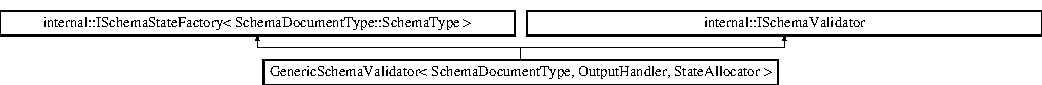
\includegraphics[height=1.135903cm]{classGenericSchemaValidator}
\end{center}
\end{figure}
\subsection*{Public Types}
\begin{DoxyCompactItemize}
\item 
typedef Schema\+Document\+Type\+::\+Schema\+Type {\bfseries Schema\+Type}\hypertarget{classGenericSchemaValidator_ac79628f00f6720bbabb70b44f0d076a0}{}\label{classGenericSchemaValidator_ac79628f00f6720bbabb70b44f0d076a0}

\item 
typedef Schema\+Document\+Type\+::\+Pointer\+Type {\bfseries Pointer\+Type}\hypertarget{classGenericSchemaValidator_ae0c6c9a9c0ff6bae80e75c6705f2668b}{}\label{classGenericSchemaValidator_ae0c6c9a9c0ff6bae80e75c6705f2668b}

\item 
typedef Schema\+Type\+::\+Encoding\+Type {\bfseries Encoding\+Type}\hypertarget{classGenericSchemaValidator_acf1c5361bb96da87d23167d8720b1ea5}{}\label{classGenericSchemaValidator_acf1c5361bb96da87d23167d8720b1ea5}

\item 
typedef Encoding\+Type\+::\+Ch {\bfseries Ch}\hypertarget{classGenericSchemaValidator_a8b7dab5a0cda9cc0adaefb4401d260c1}{}\label{classGenericSchemaValidator_a8b7dab5a0cda9cc0adaefb4401d260c1}

\end{DoxyCompactItemize}
\subsection*{Public Member Functions}
\begin{DoxyCompactItemize}
\item 
\hyperlink{classGenericSchemaValidator_a202ee6fdbe5ae9eab3e77a81ecdfeb6d}{Generic\+Schema\+Validator} (const Schema\+Document\+Type \&schema\+Document, State\+Allocator $\ast$allocator=0, size\+\_\+t schema\+Stack\+Capacity=k\+Default\+Schema\+Stack\+Capacity, size\+\_\+t document\+Stack\+Capacity=k\+Default\+Document\+Stack\+Capacity)
\begin{DoxyCompactList}\small\item\em Constructor without output handler. \end{DoxyCompactList}\item 
\hyperlink{classGenericSchemaValidator_ac2027be8ca55b01cd6f38b45f4e233b4}{Generic\+Schema\+Validator} (const Schema\+Document\+Type \&schema\+Document, Output\+Handler \&output\+Handler, State\+Allocator $\ast$allocator=0, size\+\_\+t schema\+Stack\+Capacity=k\+Default\+Schema\+Stack\+Capacity, size\+\_\+t document\+Stack\+Capacity=k\+Default\+Document\+Stack\+Capacity)
\begin{DoxyCompactList}\small\item\em Constructor with output handler. \end{DoxyCompactList}\item 
\hyperlink{classGenericSchemaValidator_a3eab83d483a50efb0c0390adf3291963}{$\sim$\+Generic\+Schema\+Validator} ()\hypertarget{classGenericSchemaValidator_a3eab83d483a50efb0c0390adf3291963}{}\label{classGenericSchemaValidator_a3eab83d483a50efb0c0390adf3291963}

\begin{DoxyCompactList}\small\item\em Destructor. \end{DoxyCompactList}\item 
void \hyperlink{classGenericSchemaValidator_a49efbbe098cb77728be3d48cafed17e4}{Reset} ()\hypertarget{classGenericSchemaValidator_a49efbbe098cb77728be3d48cafed17e4}{}\label{classGenericSchemaValidator_a49efbbe098cb77728be3d48cafed17e4}

\begin{DoxyCompactList}\small\item\em Reset the internal states. \end{DoxyCompactList}\item 
virtual bool \hyperlink{classGenericSchemaValidator_ae1559e9448b51a2de30cd39d431179f4}{Is\+Valid} () const \hypertarget{classGenericSchemaValidator_ae1559e9448b51a2de30cd39d431179f4}{}\label{classGenericSchemaValidator_ae1559e9448b51a2de30cd39d431179f4}

\begin{DoxyCompactList}\small\item\em Checks whether the current state is valid. \end{DoxyCompactList}\item 
Pointer\+Type \hyperlink{classGenericSchemaValidator_a39879de53c70fd5d3c018b61d1235681}{Get\+Invalid\+Schema\+Pointer} () const \hypertarget{classGenericSchemaValidator_a39879de53c70fd5d3c018b61d1235681}{}\label{classGenericSchemaValidator_a39879de53c70fd5d3c018b61d1235681}

\begin{DoxyCompactList}\small\item\em Gets the J\+S\+ON pointer pointed to the invalid schema. \end{DoxyCompactList}\item 
const Ch $\ast$ \hyperlink{classGenericSchemaValidator_a016b23047ed66bac570e378fbaaf839b}{Get\+Invalid\+Schema\+Keyword} () const \hypertarget{classGenericSchemaValidator_a016b23047ed66bac570e378fbaaf839b}{}\label{classGenericSchemaValidator_a016b23047ed66bac570e378fbaaf839b}

\begin{DoxyCompactList}\small\item\em Gets the keyword of invalid schema. \end{DoxyCompactList}\item 
Pointer\+Type \hyperlink{classGenericSchemaValidator_ae65727ef84d82f3e31e1f57543e71320}{Get\+Invalid\+Document\+Pointer} () const \hypertarget{classGenericSchemaValidator_ae65727ef84d82f3e31e1f57543e71320}{}\label{classGenericSchemaValidator_ae65727ef84d82f3e31e1f57543e71320}

\begin{DoxyCompactList}\small\item\em Gets the J\+S\+ON pointer pointed to the invalid value. \end{DoxyCompactList}\item 
bool {\bfseries Null} ()\hypertarget{classGenericSchemaValidator_a7137af73e934f50c66cbb8a9aa802ea6}{}\label{classGenericSchemaValidator_a7137af73e934f50c66cbb8a9aa802ea6}

\item 
bool {\bfseries Bool} (bool b)\hypertarget{classGenericSchemaValidator_aa25fa7456f2f308a105e400f01a4afde}{}\label{classGenericSchemaValidator_aa25fa7456f2f308a105e400f01a4afde}

\item 
bool {\bfseries Int} (int i)\hypertarget{classGenericSchemaValidator_ad823c29990225661a4df69d34647b659}{}\label{classGenericSchemaValidator_ad823c29990225661a4df69d34647b659}

\item 
bool {\bfseries Uint} (unsigned u)\hypertarget{classGenericSchemaValidator_aa688665c5274f93543c84a4b6cabe8da}{}\label{classGenericSchemaValidator_aa688665c5274f93543c84a4b6cabe8da}

\item 
bool {\bfseries Int64} (int64\+\_\+t i)\hypertarget{classGenericSchemaValidator_ac5a9e416e18129a7b787f251019a828f}{}\label{classGenericSchemaValidator_ac5a9e416e18129a7b787f251019a828f}

\item 
bool {\bfseries Uint64} (uint64\+\_\+t u)\hypertarget{classGenericSchemaValidator_abfc56c58cf0b65318e376fc5f2879292}{}\label{classGenericSchemaValidator_abfc56c58cf0b65318e376fc5f2879292}

\item 
bool {\bfseries Double} (double d)\hypertarget{classGenericSchemaValidator_aed0532dbda3ac6f3ca7196af06066b86}{}\label{classGenericSchemaValidator_aed0532dbda3ac6f3ca7196af06066b86}

\item 
bool {\bfseries Raw\+Number} (const Ch $\ast$str, \hyperlink{rapidjson_8h_a5ed6e6e67250fadbd041127e6386dcb5}{Size\+Type} length, bool copy)\hypertarget{classGenericSchemaValidator_ae4f024145421d2c1dde08a9de528722a}{}\label{classGenericSchemaValidator_ae4f024145421d2c1dde08a9de528722a}

\item 
bool {\bfseries String} (const Ch $\ast$str, \hyperlink{rapidjson_8h_a5ed6e6e67250fadbd041127e6386dcb5}{Size\+Type} length, bool copy)\hypertarget{classGenericSchemaValidator_a33cf3f83307a8fea38c3238ef75c3d58}{}\label{classGenericSchemaValidator_a33cf3f83307a8fea38c3238ef75c3d58}

\item 
bool {\bfseries Start\+Object} ()\hypertarget{classGenericSchemaValidator_a59972d612c3d37aae9a30222e428d216}{}\label{classGenericSchemaValidator_a59972d612c3d37aae9a30222e428d216}

\item 
bool {\bfseries Key} (const Ch $\ast$str, \hyperlink{rapidjson_8h_a5ed6e6e67250fadbd041127e6386dcb5}{Size\+Type} len, bool copy)\hypertarget{classGenericSchemaValidator_a6d08b458216ec4a09eed9d94800d05c1}{}\label{classGenericSchemaValidator_a6d08b458216ec4a09eed9d94800d05c1}

\item 
bool {\bfseries End\+Object} (\hyperlink{rapidjson_8h_a5ed6e6e67250fadbd041127e6386dcb5}{Size\+Type} member\+Count)\hypertarget{classGenericSchemaValidator_aa89e14f0f731f6acdec22a0f7e003037}{}\label{classGenericSchemaValidator_aa89e14f0f731f6acdec22a0f7e003037}

\item 
bool {\bfseries Start\+Array} ()\hypertarget{classGenericSchemaValidator_aba13751f802531ed8cbd850778ea993c}{}\label{classGenericSchemaValidator_aba13751f802531ed8cbd850778ea993c}

\item 
bool {\bfseries End\+Array} (\hyperlink{rapidjson_8h_a5ed6e6e67250fadbd041127e6386dcb5}{Size\+Type} element\+Count)\hypertarget{classGenericSchemaValidator_a67b501f0f65d40e0086ca8216882b34f}{}\label{classGenericSchemaValidator_a67b501f0f65d40e0086ca8216882b34f}

\item 
virtual I\+Schema\+Validator $\ast$ {\bfseries Create\+Schema\+Validator} (const Schema\+Type \&root)\hypertarget{classGenericSchemaValidator_af074f9c8f2cfc07e1b3d3f8862e7ef11}{}\label{classGenericSchemaValidator_af074f9c8f2cfc07e1b3d3f8862e7ef11}

\item 
virtual void {\bfseries Destroy\+Schema\+Validator} (I\+Schema\+Validator $\ast$validator)\hypertarget{classGenericSchemaValidator_ae24fa298e328f1fd7dda2ef6267156d2}{}\label{classGenericSchemaValidator_ae24fa298e328f1fd7dda2ef6267156d2}

\item 
virtual void $\ast$ {\bfseries Create\+Hasher} ()\hypertarget{classGenericSchemaValidator_abc377481583ca2095fb784be88887faa}{}\label{classGenericSchemaValidator_abc377481583ca2095fb784be88887faa}

\item 
virtual uint64\+\_\+t {\bfseries Get\+Hash\+Code} (void $\ast$hasher)\hypertarget{classGenericSchemaValidator_ac01c45982a1f512e1ca06fe5544b0c0f}{}\label{classGenericSchemaValidator_ac01c45982a1f512e1ca06fe5544b0c0f}

\item 
virtual void {\bfseries Destrory\+Hasher} (void $\ast$hasher)\hypertarget{classGenericSchemaValidator_a007eef58be575dc562543d069ddd2710}{}\label{classGenericSchemaValidator_a007eef58be575dc562543d069ddd2710}

\item 
virtual void $\ast$ {\bfseries Malloc\+State} (size\+\_\+t size)\hypertarget{classGenericSchemaValidator_a7c999dfb3118aaa08495d60eee6d3732}{}\label{classGenericSchemaValidator_a7c999dfb3118aaa08495d60eee6d3732}

\item 
virtual void {\bfseries Free\+State} (void $\ast$p)\hypertarget{classGenericSchemaValidator_a4e250737a411af2969a9e585a7da4187}{}\label{classGenericSchemaValidator_a4e250737a411af2969a9e585a7da4187}

\end{DoxyCompactItemize}


\subsection{Detailed Description}
\subsubsection*{template$<$typename Schema\+Document\+Type, typename Output\+Handler = Base\+Reader\+Handler$<$typename Schema\+Document\+Type\+::\+Schema\+Type\+::\+Encoding\+Type$>$, typename State\+Allocator = Crt\+Allocator$>$\\*
class Generic\+Schema\+Validator$<$ Schema\+Document\+Type, Output\+Handler, State\+Allocator $>$}

J\+S\+ON Schema Validator. 

A S\+AX style J\+S\+ON schema validator. It uses a {\ttfamily \hyperlink{classGenericSchemaDocument}{Generic\+Schema\+Document}} to validate S\+AX events. It delegates the incoming S\+AX events to an output handler. The default output handler does nothing. It can be reused multiple times by calling {\ttfamily \hyperlink{classGenericSchemaValidator_a49efbbe098cb77728be3d48cafed17e4}{Reset()}}.


\begin{DoxyTemplParams}{Template Parameters}
{\em Schema\+Document\+Type} & Type of schema document. \\
\hline
{\em Output\+Handler} & Type of output handler. Default handler does nothing. \\
\hline
{\em State\+Allocator} & Allocator for storing the internal validation states. \\
\hline
\end{DoxyTemplParams}


\subsection{Constructor \& Destructor Documentation}
\index{Generic\+Schema\+Validator@{Generic\+Schema\+Validator}!Generic\+Schema\+Validator@{Generic\+Schema\+Validator}}
\index{Generic\+Schema\+Validator@{Generic\+Schema\+Validator}!Generic\+Schema\+Validator@{Generic\+Schema\+Validator}}
\subsubsection[{\texorpdfstring{Generic\+Schema\+Validator(const Schema\+Document\+Type \&schema\+Document, State\+Allocator $\ast$allocator=0, size\+\_\+t schema\+Stack\+Capacity=k\+Default\+Schema\+Stack\+Capacity, size\+\_\+t document\+Stack\+Capacity=k\+Default\+Document\+Stack\+Capacity)}{GenericSchemaValidator(const SchemaDocumentType &schemaDocument, StateAllocator *allocator=0, size_t schemaStackCapacity=kDefaultSchemaStackCapacity, size_t documentStackCapacity=kDefaultDocumentStackCapacity)}}]{\setlength{\rightskip}{0pt plus 5cm}template$<$typename Schema\+Document\+Type, typename Output\+Handler = Base\+Reader\+Handler$<$typename Schema\+Document\+Type\+::\+Schema\+Type\+::\+Encoding\+Type$>$, typename State\+Allocator = Crt\+Allocator$>$ {\bf Generic\+Schema\+Validator}$<$ Schema\+Document\+Type, Output\+Handler, State\+Allocator $>$\+::{\bf Generic\+Schema\+Validator} (
\begin{DoxyParamCaption}
\item[{const Schema\+Document\+Type \&}]{schema\+Document, }
\item[{State\+Allocator $\ast$}]{allocator = {\ttfamily 0}, }
\item[{size\+\_\+t}]{schema\+Stack\+Capacity = {\ttfamily kDefaultSchemaStackCapacity}, }
\item[{size\+\_\+t}]{document\+Stack\+Capacity = {\ttfamily kDefaultDocumentStackCapacity}}
\end{DoxyParamCaption}
)\hspace{0.3cm}{\ttfamily [inline]}}\hypertarget{classGenericSchemaValidator_a202ee6fdbe5ae9eab3e77a81ecdfeb6d}{}\label{classGenericSchemaValidator_a202ee6fdbe5ae9eab3e77a81ecdfeb6d}


Constructor without output handler. 


\begin{DoxyParams}{Parameters}
{\em schema\+Document} & The schema document to conform to. \\
\hline
{\em allocator} & Optional allocator for storing internal validation states. \\
\hline
{\em schema\+Stack\+Capacity} & Optional initial capacity of schema path stack. \\
\hline
{\em document\+Stack\+Capacity} & Optional initial capacity of document path stack. \\
\hline
\end{DoxyParams}
\index{Generic\+Schema\+Validator@{Generic\+Schema\+Validator}!Generic\+Schema\+Validator@{Generic\+Schema\+Validator}}
\index{Generic\+Schema\+Validator@{Generic\+Schema\+Validator}!Generic\+Schema\+Validator@{Generic\+Schema\+Validator}}
\subsubsection[{\texorpdfstring{Generic\+Schema\+Validator(const Schema\+Document\+Type \&schema\+Document, Output\+Handler \&output\+Handler, State\+Allocator $\ast$allocator=0, size\+\_\+t schema\+Stack\+Capacity=k\+Default\+Schema\+Stack\+Capacity, size\+\_\+t document\+Stack\+Capacity=k\+Default\+Document\+Stack\+Capacity)}{GenericSchemaValidator(const SchemaDocumentType &schemaDocument, OutputHandler &outputHandler, StateAllocator *allocator=0, size_t schemaStackCapacity=kDefaultSchemaStackCapacity, size_t documentStackCapacity=kDefaultDocumentStackCapacity)}}]{\setlength{\rightskip}{0pt plus 5cm}template$<$typename Schema\+Document\+Type, typename Output\+Handler = Base\+Reader\+Handler$<$typename Schema\+Document\+Type\+::\+Schema\+Type\+::\+Encoding\+Type$>$, typename State\+Allocator = Crt\+Allocator$>$ {\bf Generic\+Schema\+Validator}$<$ Schema\+Document\+Type, Output\+Handler, State\+Allocator $>$\+::{\bf Generic\+Schema\+Validator} (
\begin{DoxyParamCaption}
\item[{const Schema\+Document\+Type \&}]{schema\+Document, }
\item[{Output\+Handler \&}]{output\+Handler, }
\item[{State\+Allocator $\ast$}]{allocator = {\ttfamily 0}, }
\item[{size\+\_\+t}]{schema\+Stack\+Capacity = {\ttfamily kDefaultSchemaStackCapacity}, }
\item[{size\+\_\+t}]{document\+Stack\+Capacity = {\ttfamily kDefaultDocumentStackCapacity}}
\end{DoxyParamCaption}
)\hspace{0.3cm}{\ttfamily [inline]}}\hypertarget{classGenericSchemaValidator_ac2027be8ca55b01cd6f38b45f4e233b4}{}\label{classGenericSchemaValidator_ac2027be8ca55b01cd6f38b45f4e233b4}


Constructor with output handler. 


\begin{DoxyParams}{Parameters}
{\em schema\+Document} & The schema document to conform to. \\
\hline
{\em allocator} & Optional allocator for storing internal validation states. \\
\hline
{\em schema\+Stack\+Capacity} & Optional initial capacity of schema path stack. \\
\hline
{\em document\+Stack\+Capacity} & Optional initial capacity of document path stack. \\
\hline
\end{DoxyParams}


The documentation for this class was generated from the following files\+:\begin{DoxyCompactItemize}
\item 
/home/mate/\+Documents/\+Programming/\+Research/\+Multilayer\+Network\+Model/\+Multilayer\+Network\+Model/sources/external/rapidjson/fwd.\+h\item 
/home/mate/\+Documents/\+Programming/\+Research/\+Multilayer\+Network\+Model/\+Multilayer\+Network\+Model/sources/external/rapidjson/schema.\+h\end{DoxyCompactItemize}

\hypertarget{classGenericStreamWrapper}{}\section{Generic\+Stream\+Wrapper$<$ Input\+Stream, Encoding $>$ Class Template Reference}
\label{classGenericStreamWrapper}\index{Generic\+Stream\+Wrapper$<$ Input\+Stream, Encoding $>$@{Generic\+Stream\+Wrapper$<$ Input\+Stream, Encoding $>$}}


A Stream Wrapper.  




{\ttfamily \#include $<$stream.\+h$>$}

Inheritance diagram for Generic\+Stream\+Wrapper$<$ Input\+Stream, Encoding $>$\+:\begin{figure}[H]
\begin{center}
\leavevmode
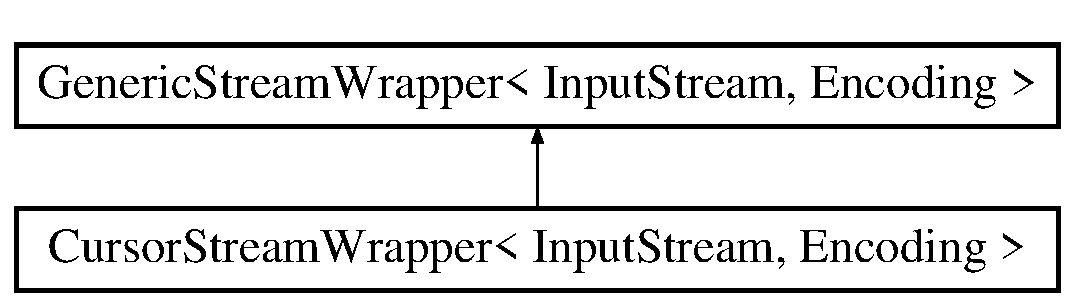
\includegraphics[height=2.000000cm]{classGenericStreamWrapper}
\end{center}
\end{figure}
\subsection*{Public Types}
\begin{DoxyCompactItemize}
\item 
typedef Encoding\+::\+Ch {\bfseries Ch}\hypertarget{classGenericStreamWrapper_aef9e89bc4997497315bde1b60e8bb848}{}\label{classGenericStreamWrapper_aef9e89bc4997497315bde1b60e8bb848}

\end{DoxyCompactItemize}
\subsection*{Public Member Functions}
\begin{DoxyCompactItemize}
\item 
{\bfseries Generic\+Stream\+Wrapper} (Input\+Stream \&is)\hypertarget{classGenericStreamWrapper_a7b12b1de6337d3f8e635b650e372c803}{}\label{classGenericStreamWrapper_a7b12b1de6337d3f8e635b650e372c803}

\item 
Ch {\bfseries Peek} () const \hypertarget{classGenericStreamWrapper_a67b469da031928fb159d0c3b706f44d7}{}\label{classGenericStreamWrapper_a67b469da031928fb159d0c3b706f44d7}

\item 
Ch {\bfseries Take} ()\hypertarget{classGenericStreamWrapper_a1c0bc67a233e08ed89b4ff37455e7754}{}\label{classGenericStreamWrapper_a1c0bc67a233e08ed89b4ff37455e7754}

\item 
size\+\_\+t {\bfseries Tell} ()\hypertarget{classGenericStreamWrapper_a5068a627e0a2deffa985db39f89c5378}{}\label{classGenericStreamWrapper_a5068a627e0a2deffa985db39f89c5378}

\item 
Ch $\ast$ {\bfseries Put\+Begin} ()\hypertarget{classGenericStreamWrapper_a4b35b8e9b6feba4d7f1d99ffce17f83d}{}\label{classGenericStreamWrapper_a4b35b8e9b6feba4d7f1d99ffce17f83d}

\item 
void {\bfseries Put} (Ch ch)\hypertarget{classGenericStreamWrapper_a458b9f3e00ad41dadb069839ab53f0ba}{}\label{classGenericStreamWrapper_a458b9f3e00ad41dadb069839ab53f0ba}

\item 
void {\bfseries Flush} ()\hypertarget{classGenericStreamWrapper_a210c0864fbff3cc72f2f62ed461105fb}{}\label{classGenericStreamWrapper_a210c0864fbff3cc72f2f62ed461105fb}

\item 
size\+\_\+t {\bfseries Put\+End} (Ch $\ast$ch)\hypertarget{classGenericStreamWrapper_a84f8d6e1f95d53c4e8e22892d5113fd3}{}\label{classGenericStreamWrapper_a84f8d6e1f95d53c4e8e22892d5113fd3}

\item 
const Ch $\ast$ {\bfseries Peek4} () const \hypertarget{classGenericStreamWrapper_af3eb96763744e85075cc221b5840cda3}{}\label{classGenericStreamWrapper_af3eb96763744e85075cc221b5840cda3}

\item 
U\+T\+F\+Type {\bfseries Get\+Type} () const \hypertarget{classGenericStreamWrapper_aad72e81846f45d922f8f172b9842c7bb}{}\label{classGenericStreamWrapper_aad72e81846f45d922f8f172b9842c7bb}

\item 
bool {\bfseries Has\+B\+OM} () const \hypertarget{classGenericStreamWrapper_a6ebd59bda5fc5754d71731416a88906b}{}\label{classGenericStreamWrapper_a6ebd59bda5fc5754d71731416a88906b}

\end{DoxyCompactItemize}
\subsection*{Protected Attributes}
\begin{DoxyCompactItemize}
\item 
Input\+Stream \& {\bfseries is\+\_\+}\hypertarget{classGenericStreamWrapper_a2b44ae2c9460c2e18aca6ba25c537cc5}{}\label{classGenericStreamWrapper_a2b44ae2c9460c2e18aca6ba25c537cc5}

\end{DoxyCompactItemize}


\subsection{Detailed Description}
\subsubsection*{template$<$typename Input\+Stream, typename Encoding = U\+T\+F8$<$$>$$>$\\*
class Generic\+Stream\+Wrapper$<$ Input\+Stream, Encoding $>$}

A Stream Wrapper. 

string stream is a wrapper for any stream by just forwarding any  message to the origin stream. \begin{DoxyNote}{Note}
implements Stream concept 
\end{DoxyNote}


The documentation for this class was generated from the following file\+:\begin{DoxyCompactItemize}
\item 
/home/mate/\+Documents/\+Programming/\+Research/\+Multilayer\+Network\+Model/\+Multilayer\+Network\+Model/sources/external/rapidjson/stream.\+h\end{DoxyCompactItemize}

\hypertarget{classGenericStringBuffer}{}\section{Generic\+String\+Buffer$<$ Encoding, Allocator $>$ Class Template Reference}
\label{classGenericStringBuffer}\index{Generic\+String\+Buffer$<$ Encoding, Allocator $>$@{Generic\+String\+Buffer$<$ Encoding, Allocator $>$}}


Represents an in-\/memory output stream.  




{\ttfamily \#include $<$stringbuffer.\+h$>$}

\subsection*{Public Types}
\begin{DoxyCompactItemize}
\item 
typedef Encoding\+::\+Ch {\bfseries Ch}\hypertarget{classGenericStringBuffer_a735b75db076ffe86d0d294be49655d46}{}\label{classGenericStringBuffer_a735b75db076ffe86d0d294be49655d46}

\end{DoxyCompactItemize}
\subsection*{Public Member Functions}
\begin{DoxyCompactItemize}
\item 
{\bfseries Generic\+String\+Buffer} (Allocator $\ast$allocator=0, size\+\_\+t capacity=k\+Default\+Capacity)\hypertarget{classGenericStringBuffer_a62f5ea1a53a2a3f98088f8c152b6183e}{}\label{classGenericStringBuffer_a62f5ea1a53a2a3f98088f8c152b6183e}

\item 
void {\bfseries Put} (Ch c)\hypertarget{classGenericStringBuffer_a8be5c8fadccacdcf40e20220f38e0afa}{}\label{classGenericStringBuffer_a8be5c8fadccacdcf40e20220f38e0afa}

\item 
void {\bfseries Put\+Unsafe} (Ch c)\hypertarget{classGenericStringBuffer_a9225468d11fdddfc3a9a4e48bf4d3ba4}{}\label{classGenericStringBuffer_a9225468d11fdddfc3a9a4e48bf4d3ba4}

\item 
void {\bfseries Flush} ()\hypertarget{classGenericStringBuffer_a28bb539487db17b07314a532f3b8847c}{}\label{classGenericStringBuffer_a28bb539487db17b07314a532f3b8847c}

\item 
void {\bfseries Clear} ()\hypertarget{classGenericStringBuffer_a42f15c959046d899cb74c3120a6995f9}{}\label{classGenericStringBuffer_a42f15c959046d899cb74c3120a6995f9}

\item 
void {\bfseries Shrink\+To\+Fit} ()\hypertarget{classGenericStringBuffer_a0dbdb77489b95923795011a24f705be5}{}\label{classGenericStringBuffer_a0dbdb77489b95923795011a24f705be5}

\item 
void {\bfseries Reserve} (size\+\_\+t count)\hypertarget{classGenericStringBuffer_a4d6becae201b98c122746298882a318f}{}\label{classGenericStringBuffer_a4d6becae201b98c122746298882a318f}

\item 
Ch $\ast$ {\bfseries Push} (size\+\_\+t count)\hypertarget{classGenericStringBuffer_a49fd10cdd5dd97a4cf9813d01334d660}{}\label{classGenericStringBuffer_a49fd10cdd5dd97a4cf9813d01334d660}

\item 
Ch $\ast$ {\bfseries Push\+Unsafe} (size\+\_\+t count)\hypertarget{classGenericStringBuffer_a4e396f55323ca54f949685c7c6ef2060}{}\label{classGenericStringBuffer_a4e396f55323ca54f949685c7c6ef2060}

\item 
void {\bfseries Pop} (size\+\_\+t count)\hypertarget{classGenericStringBuffer_a0038e53ba03c271bc4cbbac403ec4de4}{}\label{classGenericStringBuffer_a0038e53ba03c271bc4cbbac403ec4de4}

\item 
const Ch $\ast$ {\bfseries Get\+String} () const \hypertarget{classGenericStringBuffer_a42ed917a29012d932802f2709e11c572}{}\label{classGenericStringBuffer_a42ed917a29012d932802f2709e11c572}

\item 
size\+\_\+t \hyperlink{classGenericStringBuffer_abd04725d776322157be3381f5559c40b}{Get\+Size} () const \hypertarget{classGenericStringBuffer_abd04725d776322157be3381f5559c40b}{}\label{classGenericStringBuffer_abd04725d776322157be3381f5559c40b}

\begin{DoxyCompactList}\small\item\em Get the size of string in bytes in the string buffer. \end{DoxyCompactList}\item 
size\+\_\+t \hyperlink{classGenericStringBuffer_a8ad04ebc2bbe46a116613d1ed0d1eeff}{Get\+Length} () const \hypertarget{classGenericStringBuffer_a8ad04ebc2bbe46a116613d1ed0d1eeff}{}\label{classGenericStringBuffer_a8ad04ebc2bbe46a116613d1ed0d1eeff}

\begin{DoxyCompactList}\small\item\em Get the length of string in Ch in the string buffer. \end{DoxyCompactList}\end{DoxyCompactItemize}
\subsection*{Public Attributes}
\begin{DoxyCompactItemize}
\item 
\hyperlink{classinternal_1_1Stack}{internal\+::\+Stack}$<$ Allocator $>$ {\bfseries stack\+\_\+}\hypertarget{classGenericStringBuffer_aaef716643febb9de5957dbf8ff904409}{}\label{classGenericStringBuffer_aaef716643febb9de5957dbf8ff904409}

\end{DoxyCompactItemize}
\subsection*{Static Public Attributes}
\begin{DoxyCompactItemize}
\item 
static const size\+\_\+t {\bfseries k\+Default\+Capacity} = 256\hypertarget{classGenericStringBuffer_ae74f9df854dd5a7db4315ef44b016d22}{}\label{classGenericStringBuffer_ae74f9df854dd5a7db4315ef44b016d22}

\end{DoxyCompactItemize}


\subsection{Detailed Description}
\subsubsection*{template$<$typename Encoding, typename Allocator = Crt\+Allocator$>$\\*
class Generic\+String\+Buffer$<$ Encoding, Allocator $>$}

Represents an in-\/memory output stream. 


\begin{DoxyTemplParams}{Template Parameters}
{\em Encoding} & Encoding of the stream. \\
\hline
{\em Allocator} & type for allocating memory buffer. \\
\hline
\end{DoxyTemplParams}
\begin{DoxyNote}{Note}
implements Stream concept 
\end{DoxyNote}


The documentation for this class was generated from the following files\+:\begin{DoxyCompactItemize}
\item 
/home/mate/\+Documents/\+Programming/\+Research/\+Multilayer\+Network\+Model/\+Multilayer\+Network\+Model/src/external/rapidjson/fwd.\+h\item 
/home/mate/\+Documents/\+Programming/\+Research/\+Multilayer\+Network\+Model/\+Multilayer\+Network\+Model/src/external/rapidjson/stringbuffer.\+h\end{DoxyCompactItemize}

\hypertarget{structGenericStringRef}{}\section{Generic\+String\+Ref$<$ Char\+Type $>$ Struct Template Reference}
\label{structGenericStringRef}\index{Generic\+String\+Ref$<$ Char\+Type $>$@{Generic\+String\+Ref$<$ Char\+Type $>$}}


Reference to a constant string (not taking a copy)  




{\ttfamily \#include $<$document.\+h$>$}

\subsection*{Public Types}
\begin{DoxyCompactItemize}
\item 
typedef Char\+Type \hyperlink{structGenericStringRef_a16908c3fce41be380061330c14ba2140}{Ch}\hypertarget{structGenericStringRef_a16908c3fce41be380061330c14ba2140}{}\label{structGenericStringRef_a16908c3fce41be380061330c14ba2140}

\begin{DoxyCompactList}\small\item\em character type of the string \end{DoxyCompactList}\end{DoxyCompactItemize}
\subsection*{Public Member Functions}
\begin{DoxyCompactItemize}
\item 
{\footnotesize template$<$Size\+Type N$>$ }\\\hyperlink{structGenericStringRef_aae0c070f914d2486a560150a927c22dc}{Generic\+String\+Ref} (const Char\+Type(\&str)\mbox{[}N\mbox{]}) R\+A\+P\+I\+D\+J\+S\+O\+N\+\_\+\+N\+O\+E\+X\+C\+E\+PT
\begin{DoxyCompactList}\small\item\em Create string reference from {\ttfamily const} character array. \end{DoxyCompactList}\item 
\hyperlink{structGenericStringRef_a9e80d81d5ad49cf0fb4128ace8c548d9}{Generic\+String\+Ref} (const Char\+Type $\ast$str)
\begin{DoxyCompactList}\small\item\em Explicitly create string reference from {\ttfamily const} character pointer. \end{DoxyCompactList}\item 
\hyperlink{structGenericStringRef_a8b2c6a7fdc4da1e7055f7fdcf0ac517f}{Generic\+String\+Ref} (const Char\+Type $\ast$str, \hyperlink{rapidjson_8h_a5ed6e6e67250fadbd041127e6386dcb5}{Size\+Type} len)
\begin{DoxyCompactList}\small\item\em Create constant string reference from pointer and length. \end{DoxyCompactList}\item 
{\bfseries Generic\+String\+Ref} (const \hyperlink{structGenericStringRef}{Generic\+String\+Ref} \&rhs)\hypertarget{structGenericStringRef_ab049693082c0b8f5066c00212e780aec}{}\label{structGenericStringRef_ab049693082c0b8f5066c00212e780aec}

\item 
\hyperlink{structGenericStringRef_a61a4241c23f65626ddc1da4ae5dac1b8}{operator const Ch $\ast$} () const \hypertarget{structGenericStringRef_a61a4241c23f65626ddc1da4ae5dac1b8}{}\label{structGenericStringRef_a61a4241c23f65626ddc1da4ae5dac1b8}

\begin{DoxyCompactList}\small\item\em implicit conversion to plain Char\+Type pointer \end{DoxyCompactList}\end{DoxyCompactItemize}
\subsection*{Public Attributes}
\begin{DoxyCompactItemize}
\item 
const \hyperlink{structGenericStringRef_a16908c3fce41be380061330c14ba2140}{Ch} $\ast$const \hyperlink{structGenericStringRef_ac555994afd329bc9bc1780acf2f9d9be}{s}\hypertarget{structGenericStringRef_ac555994afd329bc9bc1780acf2f9d9be}{}\label{structGenericStringRef_ac555994afd329bc9bc1780acf2f9d9be}

\begin{DoxyCompactList}\small\item\em plain Char\+Type pointer \end{DoxyCompactList}\item 
const \hyperlink{rapidjson_8h_a5ed6e6e67250fadbd041127e6386dcb5}{Size\+Type} \hyperlink{structGenericStringRef_a4a96d618744ad73f766a1551b1d517fe}{length}\hypertarget{structGenericStringRef_a4a96d618744ad73f766a1551b1d517fe}{}\label{structGenericStringRef_a4a96d618744ad73f766a1551b1d517fe}

\begin{DoxyCompactList}\small\item\em length of the string (excluding the trailing N\+U\+LL terminator) \end{DoxyCompactList}\end{DoxyCompactItemize}
\subsection*{Related Functions}
(Note that these are not member functions.) \begin{DoxyCompactItemize}
\item 
{\footnotesize template$<$typename Char\+Type $>$ }\\\hyperlink{structGenericStringRef}{Generic\+String\+Ref}$<$ Char\+Type $>$ \hyperlink{structGenericStringRef_aa6b9fd9f6aa49405a574c362ba9af6b5}{String\+Ref} (const Char\+Type $\ast$str)
\begin{DoxyCompactList}\small\item\em Mark a character pointer as constant string. \end{DoxyCompactList}\item 
{\footnotesize template$<$typename Char\+Type $>$ }\\\hyperlink{structGenericStringRef}{Generic\+String\+Ref}$<$ Char\+Type $>$ \hyperlink{structGenericStringRef_a578c51ab574a50a9c760b9da7c7562f2}{String\+Ref} (const Char\+Type $\ast$str, size\+\_\+t \hyperlink{structGenericStringRef_a4a96d618744ad73f766a1551b1d517fe}{length})
\begin{DoxyCompactList}\small\item\em Mark a character pointer as constant string. \end{DoxyCompactList}\end{DoxyCompactItemize}


\subsection{Detailed Description}
\subsubsection*{template$<$typename Char\+Type$>$\\*
struct Generic\+String\+Ref$<$ Char\+Type $>$}

Reference to a constant string (not taking a copy) 


\begin{DoxyTemplParams}{Template Parameters}
{\em Char\+Type} & character type of the string\\
\hline
\end{DoxyTemplParams}
This helper class is used to automatically infer constant string references for string literals, especially from {\ttfamily const} {\bfseries }(!) character arrays.

The main use is for creating J\+S\+ON string values without copying the source string via an Allocator. This requires that the referenced string pointers have a sufficient lifetime, which exceeds the lifetime of the associated \hyperlink{classGenericValue}{Generic\+Value}.

{\bfseries Example} 
\begin{DoxyCode}
\hyperlink{classGenericValue}{Value} v(\textcolor{stringliteral}{"foo"});   \textcolor{comment}{// ok, no need to copy & calculate length}
\textcolor{keyword}{const} \textcolor{keywordtype}{char} foo[] = \textcolor{stringliteral}{"foo"};
v.SetString(foo); \textcolor{comment}{// ok}

\textcolor{keyword}{const} \textcolor{keywordtype}{char}* bar = foo;
\textcolor{comment}{// Value x(bar); // not ok, can't rely on bar's lifetime}
\hyperlink{classGenericValue}{Value} x(\hyperlink{structGenericStringRef_aa6b9fd9f6aa49405a574c362ba9af6b5}{StringRef}(bar)); \textcolor{comment}{// lifetime explicitly guaranteed by user}
\hyperlink{classGenericValue}{Value} y(\hyperlink{structGenericStringRef_aa6b9fd9f6aa49405a574c362ba9af6b5}{StringRef}(bar, 3));  \textcolor{comment}{// ok, explicitly pass length}
\end{DoxyCode}


\begin{DoxySeeAlso}{See also}
\hyperlink{structGenericStringRef_aa6b9fd9f6aa49405a574c362ba9af6b5}{String\+Ref}, Generic\+Value\+::\+Set\+String 
\end{DoxySeeAlso}


\subsection{Constructor \& Destructor Documentation}
\index{Generic\+String\+Ref@{Generic\+String\+Ref}!Generic\+String\+Ref@{Generic\+String\+Ref}}
\index{Generic\+String\+Ref@{Generic\+String\+Ref}!Generic\+String\+Ref@{Generic\+String\+Ref}}
\subsubsection[{\texorpdfstring{Generic\+String\+Ref(const Char\+Type(\&str)[N]) R\+A\+P\+I\+D\+J\+S\+O\+N\+\_\+\+N\+O\+E\+X\+C\+E\+PT}{GenericStringRef(const CharType(&str)[N]) RAPIDJSON_NOEXCEPT}}]{\setlength{\rightskip}{0pt plus 5cm}template$<$typename Char\+Type$>$ template$<$Size\+Type N$>$ {\bf Generic\+String\+Ref}$<$ Char\+Type $>$\+::{\bf Generic\+String\+Ref} (
\begin{DoxyParamCaption}
\item[{const Char\+Type(\&)}]{str\mbox{[}\+N\mbox{]}}
\end{DoxyParamCaption}
)\hspace{0.3cm}{\ttfamily [inline]}}\hypertarget{structGenericStringRef_aae0c070f914d2486a560150a927c22dc}{}\label{structGenericStringRef_aae0c070f914d2486a560150a927c22dc}


Create string reference from {\ttfamily const} character array. 

This constructor implicitly creates a constant string reference from a {\ttfamily const} character array. It has better performance than \hyperlink{structGenericStringRef_aa6b9fd9f6aa49405a574c362ba9af6b5}{String\+Ref(const Char\+Type$\ast$)} by inferring the string \hyperlink{structGenericStringRef_a4a96d618744ad73f766a1551b1d517fe}{length} from the array length, and also supports strings containing null characters.


\begin{DoxyTemplParams}{Template Parameters}
{\em N} & length of the string, automatically inferred\\
\hline
\end{DoxyTemplParams}

\begin{DoxyParams}{Parameters}
{\em str} & Constant character array, lifetime assumed to be longer than the use of the string in e.\+g. a \hyperlink{classGenericValue}{Generic\+Value}\\
\hline
\end{DoxyParams}
\begin{DoxyPostcond}{Postcondition}
\hyperlink{structGenericStringRef_ac555994afd329bc9bc1780acf2f9d9be}{s} == str
\end{DoxyPostcond}
\begin{DoxyNote}{Note}
Constant complexity. 

There is a hidden, private overload to disallow references to non-\/const character arrays to be created via this constructor. By this, e.\+g. function-\/scope arrays used to be filled via {\ttfamily snprintf} are excluded from consideration. In such cases, the referenced string should be {\bfseries copied} to the \hyperlink{classGenericValue}{Generic\+Value} instead. 
\end{DoxyNote}
\index{Generic\+String\+Ref@{Generic\+String\+Ref}!Generic\+String\+Ref@{Generic\+String\+Ref}}
\index{Generic\+String\+Ref@{Generic\+String\+Ref}!Generic\+String\+Ref@{Generic\+String\+Ref}}
\subsubsection[{\texorpdfstring{Generic\+String\+Ref(const Char\+Type $\ast$str)}{GenericStringRef(const CharType *str)}}]{\setlength{\rightskip}{0pt plus 5cm}template$<$typename Char\+Type$>$ {\bf Generic\+String\+Ref}$<$ Char\+Type $>$\+::{\bf Generic\+String\+Ref} (
\begin{DoxyParamCaption}
\item[{const Char\+Type $\ast$}]{str}
\end{DoxyParamCaption}
)\hspace{0.3cm}{\ttfamily [inline]}, {\ttfamily [explicit]}}\hypertarget{structGenericStringRef_a9e80d81d5ad49cf0fb4128ace8c548d9}{}\label{structGenericStringRef_a9e80d81d5ad49cf0fb4128ace8c548d9}


Explicitly create string reference from {\ttfamily const} character pointer. 

This constructor can be used to {\bfseries explicitly} create a reference to a constant string pointer.

\begin{DoxySeeAlso}{See also}
\hyperlink{structGenericStringRef_aa6b9fd9f6aa49405a574c362ba9af6b5}{String\+Ref(const Char\+Type$\ast$)}
\end{DoxySeeAlso}

\begin{DoxyParams}{Parameters}
{\em str} & Constant character pointer, lifetime assumed to be longer than the use of the string in e.\+g. a \hyperlink{classGenericValue}{Generic\+Value}\\
\hline
\end{DoxyParams}
\begin{DoxyPostcond}{Postcondition}
\hyperlink{structGenericStringRef_ac555994afd329bc9bc1780acf2f9d9be}{s} == str
\end{DoxyPostcond}
\begin{DoxyNote}{Note}
There is a hidden, private overload to disallow references to non-\/const character arrays to be created via this constructor. By this, e.\+g. function-\/scope arrays used to be filled via {\ttfamily snprintf} are excluded from consideration. In such cases, the referenced string should be {\bfseries copied} to the \hyperlink{classGenericValue}{Generic\+Value} instead. 
\end{DoxyNote}
\index{Generic\+String\+Ref@{Generic\+String\+Ref}!Generic\+String\+Ref@{Generic\+String\+Ref}}
\index{Generic\+String\+Ref@{Generic\+String\+Ref}!Generic\+String\+Ref@{Generic\+String\+Ref}}
\subsubsection[{\texorpdfstring{Generic\+String\+Ref(const Char\+Type $\ast$str, Size\+Type len)}{GenericStringRef(const CharType *str, SizeType len)}}]{\setlength{\rightskip}{0pt plus 5cm}template$<$typename Char\+Type$>$ {\bf Generic\+String\+Ref}$<$ Char\+Type $>$\+::{\bf Generic\+String\+Ref} (
\begin{DoxyParamCaption}
\item[{const Char\+Type $\ast$}]{str, }
\item[{{\bf Size\+Type}}]{len}
\end{DoxyParamCaption}
)\hspace{0.3cm}{\ttfamily [inline]}}\hypertarget{structGenericStringRef_a8b2c6a7fdc4da1e7055f7fdcf0ac517f}{}\label{structGenericStringRef_a8b2c6a7fdc4da1e7055f7fdcf0ac517f}


Create constant string reference from pointer and length. 


\begin{DoxyParams}{Parameters}
{\em str} & constant string, lifetime assumed to be longer than the use of the string in e.\+g. a \hyperlink{classGenericValue}{Generic\+Value} \\
\hline
{\em len} & length of the string, excluding the trailing N\+U\+LL terminator\\
\hline
\end{DoxyParams}
\begin{DoxyPostcond}{Postcondition}
\hyperlink{structGenericStringRef_ac555994afd329bc9bc1780acf2f9d9be}{s} == str \&\& \hyperlink{structGenericStringRef_a4a96d618744ad73f766a1551b1d517fe}{length} == len 
\end{DoxyPostcond}
\begin{DoxyNote}{Note}
Constant complexity. 
\end{DoxyNote}


\subsection{Friends And Related Function Documentation}
\index{Generic\+String\+Ref@{Generic\+String\+Ref}!String\+Ref@{String\+Ref}}
\index{String\+Ref@{String\+Ref}!Generic\+String\+Ref@{Generic\+String\+Ref}}
\subsubsection[{\texorpdfstring{String\+Ref(const Char\+Type $\ast$str)}{StringRef(const CharType *str)}}]{\setlength{\rightskip}{0pt plus 5cm}template$<$typename Char\+Type $>$ {\bf Generic\+String\+Ref}$<$ Char\+Type $>$ String\+Ref (
\begin{DoxyParamCaption}
\item[{const Char\+Type $\ast$}]{str}
\end{DoxyParamCaption}
)\hspace{0.3cm}{\ttfamily [related]}}\hypertarget{structGenericStringRef_aa6b9fd9f6aa49405a574c362ba9af6b5}{}\label{structGenericStringRef_aa6b9fd9f6aa49405a574c362ba9af6b5}


Mark a character pointer as constant string. 

Mark a plain character pointer as a \char`\"{}string literal\char`\"{}. This function can be used to avoid copying a character string to be referenced as a value in a J\+S\+ON \hyperlink{classGenericValue}{Generic\+Value} object, if the string\textquotesingle{}s lifetime is known to be valid long enough. 
\begin{DoxyTemplParams}{Template Parameters}
{\em Char\+Type} & Character type of the string \\
\hline
\end{DoxyTemplParams}

\begin{DoxyParams}{Parameters}
{\em str} & Constant string, lifetime assumed to be longer than the use of the string in e.\+g. a \hyperlink{classGenericValue}{Generic\+Value} \\
\hline
\end{DoxyParams}
\begin{DoxyReturn}{Returns}
\hyperlink{structGenericStringRef}{Generic\+String\+Ref} string reference object
\end{DoxyReturn}
\begin{DoxySeeAlso}{See also}
\hyperlink{classGenericValue_abb2887958974fef1b2b5c8e32cc72ddb}{Generic\+Value\+::\+Generic\+Value(\+String\+Ref\+Type)}, \hyperlink{classGenericValue_a386708557555e6389184de608af5e6a6}{Generic\+Value\+::operator=(\+String\+Ref\+Type)}, Generic\+Value\+::\+Set\+String(\+String\+Ref\+Type), Generic\+Value\+::\+Push\+Back(\+String\+Ref\+Type, Allocator\&), Generic\+Value\+::\+Add\+Member 
\end{DoxySeeAlso}
\index{Generic\+String\+Ref@{Generic\+String\+Ref}!String\+Ref@{String\+Ref}}
\index{String\+Ref@{String\+Ref}!Generic\+String\+Ref@{Generic\+String\+Ref}}
\subsubsection[{\texorpdfstring{String\+Ref(const Char\+Type $\ast$str, size\+\_\+t length)}{StringRef(const CharType *str, size_t length)}}]{\setlength{\rightskip}{0pt plus 5cm}template$<$typename Char\+Type $>$ {\bf Generic\+String\+Ref}$<$ Char\+Type $>$ String\+Ref (
\begin{DoxyParamCaption}
\item[{const Char\+Type $\ast$}]{str, }
\item[{size\+\_\+t}]{length}
\end{DoxyParamCaption}
)\hspace{0.3cm}{\ttfamily [related]}}\hypertarget{structGenericStringRef_a578c51ab574a50a9c760b9da7c7562f2}{}\label{structGenericStringRef_a578c51ab574a50a9c760b9da7c7562f2}


Mark a character pointer as constant string. 

Mark a plain character pointer as a \char`\"{}string literal\char`\"{}. This function can be used to avoid copying a character string to be referenced as a value in a J\+S\+ON \hyperlink{classGenericValue}{Generic\+Value} object, if the string\textquotesingle{}s lifetime is known to be valid long enough.

This version has better performance with supplied length, and also supports string containing null characters.


\begin{DoxyTemplParams}{Template Parameters}
{\em Char\+Type} & character type of the string \\
\hline
\end{DoxyTemplParams}

\begin{DoxyParams}{Parameters}
{\em str} & Constant string, lifetime assumed to be longer than the use of the string in e.\+g. a \hyperlink{classGenericValue}{Generic\+Value} \\
\hline
{\em length} & The length of source string. \\
\hline
\end{DoxyParams}
\begin{DoxyReturn}{Returns}
\hyperlink{structGenericStringRef}{Generic\+String\+Ref} string reference object 
\end{DoxyReturn}


The documentation for this struct was generated from the following file\+:\begin{DoxyCompactItemize}
\item 
/home/mate/\+Documents/\+Programming/\+Research/\+Multilayer\+Network\+Model/\+Multilayer\+Network\+Model/src/external/rapidjson/\hyperlink{document_8h}{document.\+h}\end{DoxyCompactItemize}

\hypertarget{structGenericStringStream}{}\section{Generic\+String\+Stream$<$ Encoding $>$ Struct Template Reference}
\label{structGenericStringStream}\index{Generic\+String\+Stream$<$ Encoding $>$@{Generic\+String\+Stream$<$ Encoding $>$}}


Read-\/only string stream.  




{\ttfamily \#include $<$stream.\+h$>$}

\subsection*{Public Types}
\begin{DoxyCompactItemize}
\item 
typedef Encoding\+::\+Ch {\bfseries Ch}\hypertarget{structGenericStringStream_a4289aca895330084ff3168e37e4f08bd}{}\label{structGenericStringStream_a4289aca895330084ff3168e37e4f08bd}

\end{DoxyCompactItemize}
\subsection*{Public Member Functions}
\begin{DoxyCompactItemize}
\item 
{\bfseries Generic\+String\+Stream} (const Ch $\ast$src)\hypertarget{structGenericStringStream_a6b20885ed64e33f5d081a1e83b07da06}{}\label{structGenericStringStream_a6b20885ed64e33f5d081a1e83b07da06}

\item 
Ch {\bfseries Peek} () const \hypertarget{structGenericStringStream_a87d794a70cf132f32521fb2b145ba58d}{}\label{structGenericStringStream_a87d794a70cf132f32521fb2b145ba58d}

\item 
Ch {\bfseries Take} ()\hypertarget{structGenericStringStream_a0d26e3e77e4fca64a87c2d71f48ac5e5}{}\label{structGenericStringStream_a0d26e3e77e4fca64a87c2d71f48ac5e5}

\item 
size\+\_\+t {\bfseries Tell} () const \hypertarget{structGenericStringStream_a71dde3ded678912be1ef56376a72a653}{}\label{structGenericStringStream_a71dde3ded678912be1ef56376a72a653}

\item 
Ch $\ast$ {\bfseries Put\+Begin} ()\hypertarget{structGenericStringStream_a88c908b4dac9773240ce4bca4b6dd837}{}\label{structGenericStringStream_a88c908b4dac9773240ce4bca4b6dd837}

\item 
void {\bfseries Put} (Ch)\hypertarget{structGenericStringStream_aaa59dc5313151a4125bf7840f87a33eb}{}\label{structGenericStringStream_aaa59dc5313151a4125bf7840f87a33eb}

\item 
void {\bfseries Flush} ()\hypertarget{structGenericStringStream_a5ff1a870d9334cd054cf4ca34c86ddc3}{}\label{structGenericStringStream_a5ff1a870d9334cd054cf4ca34c86ddc3}

\item 
size\+\_\+t {\bfseries Put\+End} (Ch $\ast$)\hypertarget{structGenericStringStream_a07b942bacda494afb3b2f7629cef14af}{}\label{structGenericStringStream_a07b942bacda494afb3b2f7629cef14af}

\end{DoxyCompactItemize}
\subsection*{Public Attributes}
\begin{DoxyCompactItemize}
\item 
const Ch $\ast$ \hyperlink{structGenericStringStream_aeda813798e3f2d6bfdac86afc11b6b80}{src\+\_\+}\hypertarget{structGenericStringStream_aeda813798e3f2d6bfdac86afc11b6b80}{}\label{structGenericStringStream_aeda813798e3f2d6bfdac86afc11b6b80}

\begin{DoxyCompactList}\small\item\em Current read position. \end{DoxyCompactList}\item 
const Ch $\ast$ \hyperlink{structGenericStringStream_a3c86ef1e1f0655028cb8a3afce11ee4f}{head\+\_\+}\hypertarget{structGenericStringStream_a3c86ef1e1f0655028cb8a3afce11ee4f}{}\label{structGenericStringStream_a3c86ef1e1f0655028cb8a3afce11ee4f}

\begin{DoxyCompactList}\small\item\em Original head of the string. \end{DoxyCompactList}\end{DoxyCompactItemize}


\subsection{Detailed Description}
\subsubsection*{template$<$typename Encoding$>$\\*
struct Generic\+String\+Stream$<$ Encoding $>$}

Read-\/only string stream. 

\begin{DoxyNote}{Note}
implements Stream concept 
\end{DoxyNote}


The documentation for this struct was generated from the following files\+:\begin{DoxyCompactItemize}
\item 
/home/mate/\+Documents/\+Programming/\+Research/\+Multilayer\+Network\+Model/\+Multilayer\+Network\+Model/src/external/rapidjson/fwd.\+h\item 
/home/mate/\+Documents/\+Programming/\+Research/\+Multilayer\+Network\+Model/\+Multilayer\+Network\+Model/src/external/rapidjson/stream.\+h\end{DoxyCompactItemize}

\hypertarget{classGenericValue}{}\section{Generic\+Value$<$ Encoding, Allocator $>$ Class Template Reference}
\label{classGenericValue}\index{Generic\+Value$<$ Encoding, Allocator $>$@{Generic\+Value$<$ Encoding, Allocator $>$}}


Represents a J\+S\+ON value. Use Value for \hyperlink{structUTF8}{U\+T\+F8} encoding and default allocator.  




{\ttfamily \#include $<$document.\+h$>$}

Inheritance diagram for Generic\+Value$<$ Encoding, Allocator $>$\+:\begin{figure}[H]
\begin{center}
\leavevmode
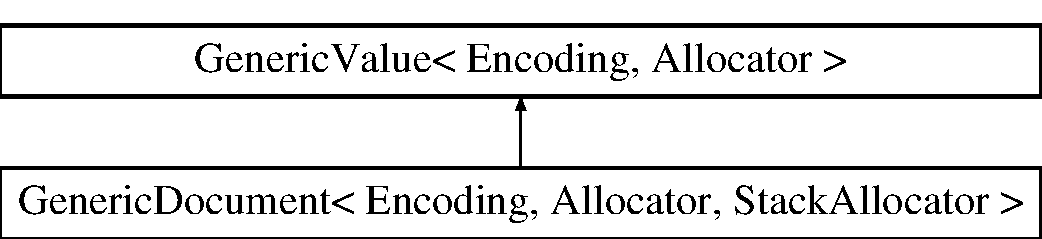
\includegraphics[height=2.000000cm]{classGenericValue}
\end{center}
\end{figure}
\subsection*{Classes}
\begin{DoxyCompactItemize}
\item 
struct \hyperlink{structGenericValue_1_1ArrayData}{Array\+Data}
\item 
union \hyperlink{unionGenericValue_1_1Data}{Data}
\item 
struct \hyperlink{structGenericValue_1_1Flag}{Flag}
\item 
union \hyperlink{unionGenericValue_1_1Number}{Number}
\item 
struct \hyperlink{structGenericValue_1_1ObjectData}{Object\+Data}
\item 
struct \hyperlink{structGenericValue_1_1ShortString}{Short\+String}
\item 
struct \hyperlink{structGenericValue_1_1String}{String}
\end{DoxyCompactItemize}
\subsection*{Public Types}
\begin{DoxyCompactItemize}
\item 
enum \{ \\*
{\bfseries k\+Bool\+Flag} = 0x0008, 
{\bfseries k\+Number\+Flag} = 0x0010, 
{\bfseries k\+Int\+Flag} = 0x0020, 
{\bfseries k\+Uint\+Flag} = 0x0040, 
\\*
{\bfseries k\+Int64\+Flag} = 0x0080, 
{\bfseries k\+Uint64\+Flag} = 0x0100, 
{\bfseries k\+Double\+Flag} = 0x0200, 
{\bfseries k\+String\+Flag} = 0x0400, 
\\*
{\bfseries k\+Copy\+Flag} = 0x0800, 
{\bfseries k\+Inline\+Str\+Flag} = 0x1000, 
{\bfseries k\+Null\+Flag} = k\+Null\+Type, 
{\bfseries k\+True\+Flag} = k\+True\+Type $\vert$ k\+Bool\+Flag, 
\\*
{\bfseries k\+False\+Flag} = k\+False\+Type $\vert$ k\+Bool\+Flag, 
{\bfseries k\+Number\+Int\+Flag} = k\+Number\+Type $\vert$ k\+Number\+Flag $\vert$ k\+Int\+Flag $\vert$ k\+Int64\+Flag, 
{\bfseries k\+Number\+Uint\+Flag} = k\+Number\+Type $\vert$ k\+Number\+Flag $\vert$ k\+Uint\+Flag $\vert$ k\+Uint64\+Flag $\vert$ k\+Int64\+Flag, 
{\bfseries k\+Number\+Int64\+Flag} = k\+Number\+Type $\vert$ k\+Number\+Flag $\vert$ k\+Int64\+Flag, 
\\*
{\bfseries k\+Number\+Uint64\+Flag} = k\+Number\+Type $\vert$ k\+Number\+Flag $\vert$ k\+Uint64\+Flag, 
{\bfseries k\+Number\+Double\+Flag} = k\+Number\+Type $\vert$ k\+Number\+Flag $\vert$ k\+Double\+Flag, 
{\bfseries k\+Number\+Any\+Flag} = k\+Number\+Type $\vert$ k\+Number\+Flag $\vert$ k\+Int\+Flag $\vert$ k\+Int64\+Flag $\vert$ k\+Uint\+Flag $\vert$ k\+Uint64\+Flag $\vert$ k\+Double\+Flag, 
{\bfseries k\+Const\+String\+Flag} = k\+String\+Type $\vert$ k\+String\+Flag, 
\\*
{\bfseries k\+Copy\+String\+Flag} = k\+String\+Type $\vert$ k\+String\+Flag $\vert$ k\+Copy\+Flag, 
{\bfseries k\+Short\+String\+Flag} = k\+String\+Type $\vert$ k\+String\+Flag $\vert$ k\+Copy\+Flag $\vert$ k\+Inline\+Str\+Flag, 
{\bfseries k\+Object\+Flag} = k\+Object\+Type, 
{\bfseries k\+Array\+Flag} = k\+Array\+Type, 
\\*
{\bfseries k\+Type\+Mask} = 0x07
 \}\hypertarget{classGenericValue_aacdfd9d0f85a6161380a134e6d0c9d3c}{}\label{classGenericValue_aacdfd9d0f85a6161380a134e6d0c9d3c}

\item 
typedef \hyperlink{structGenericMember}{Generic\+Member}$<$ Encoding, Allocator $>$ \hyperlink{classGenericValue_a7ccf27c44058b4c11c3efc6473afb886}{Member}\hypertarget{classGenericValue_a7ccf27c44058b4c11c3efc6473afb886}{}\label{classGenericValue_a7ccf27c44058b4c11c3efc6473afb886}

\begin{DoxyCompactList}\small\item\em Name-\/value pair in an object. \end{DoxyCompactList}\item 
typedef Encoding \hyperlink{classGenericValue_a28c2cb8d04d12566c1af37597a46d209}{Encoding\+Type}\hypertarget{classGenericValue_a28c2cb8d04d12566c1af37597a46d209}{}\label{classGenericValue_a28c2cb8d04d12566c1af37597a46d209}

\begin{DoxyCompactList}\small\item\em Encoding type from template parameter. \end{DoxyCompactList}\item 
typedef Allocator \hyperlink{classGenericValue_a7beb83860c1b8d2a0e2a7da9796b2fa1}{Allocator\+Type}\hypertarget{classGenericValue_a7beb83860c1b8d2a0e2a7da9796b2fa1}{}\label{classGenericValue_a7beb83860c1b8d2a0e2a7da9796b2fa1}

\begin{DoxyCompactList}\small\item\em Allocator type from template parameter. \end{DoxyCompactList}\item 
typedef Encoding\+::\+Ch \hyperlink{classGenericValue_ade0e0ce64ccd5d852da57a35e720bafb}{Ch}\hypertarget{classGenericValue_ade0e0ce64ccd5d852da57a35e720bafb}{}\label{classGenericValue_ade0e0ce64ccd5d852da57a35e720bafb}

\begin{DoxyCompactList}\small\item\em Character type derived from Encoding. \end{DoxyCompactList}\item 
typedef \hyperlink{structGenericStringRef}{Generic\+String\+Ref}$<$ \hyperlink{classGenericValue_ade0e0ce64ccd5d852da57a35e720bafb}{Ch} $>$ \hyperlink{classGenericValue_a32e0f30ee278072374c8168b14d3317f}{String\+Ref\+Type}\hypertarget{classGenericValue_a32e0f30ee278072374c8168b14d3317f}{}\label{classGenericValue_a32e0f30ee278072374c8168b14d3317f}

\begin{DoxyCompactList}\small\item\em Reference to a constant string. \end{DoxyCompactList}\item 
typedef \hyperlink{classGenericMemberIterator}{Generic\+Member\+Iterator}$<$ false, Encoding, Allocator $>$\+::Iterator \hyperlink{classGenericValue_a349b8faae61edc42b4289726820be439}{Member\+Iterator}\hypertarget{classGenericValue_a349b8faae61edc42b4289726820be439}{}\label{classGenericValue_a349b8faae61edc42b4289726820be439}

\begin{DoxyCompactList}\small\item\em Member iterator for iterating in object. \end{DoxyCompactList}\item 
typedef \hyperlink{classGenericMemberIterator}{Generic\+Member\+Iterator}$<$ true, Encoding, Allocator $>$\+::Iterator \hyperlink{classGenericValue_aac08c3e660a9036d3dcb8b10ff6c61f4}{Const\+Member\+Iterator}\hypertarget{classGenericValue_aac08c3e660a9036d3dcb8b10ff6c61f4}{}\label{classGenericValue_aac08c3e660a9036d3dcb8b10ff6c61f4}

\begin{DoxyCompactList}\small\item\em Constant member iterator for iterating in object. \end{DoxyCompactList}\item 
typedef \hyperlink{classGenericValue}{Generic\+Value} $\ast$ \hyperlink{classGenericValue_aee30721a49688ba0f865f5d581eb6be9}{Value\+Iterator}\hypertarget{classGenericValue_aee30721a49688ba0f865f5d581eb6be9}{}\label{classGenericValue_aee30721a49688ba0f865f5d581eb6be9}

\begin{DoxyCompactList}\small\item\em Value iterator for iterating in array. \end{DoxyCompactList}\item 
typedef const \hyperlink{classGenericValue}{Generic\+Value} $\ast$ \hyperlink{classGenericValue_a49010c6d6886f96ff0b0c51bccc7f6ea}{Const\+Value\+Iterator}\hypertarget{classGenericValue_a49010c6d6886f96ff0b0c51bccc7f6ea}{}\label{classGenericValue_a49010c6d6886f96ff0b0c51bccc7f6ea}

\begin{DoxyCompactList}\small\item\em Constant value iterator for iterating in array. \end{DoxyCompactList}\item 
typedef \hyperlink{classGenericValue}{Generic\+Value}$<$ Encoding, Allocator $>$ \hyperlink{classGenericValue_a43a39bb4fca9b9d3de3da6ac353d25ce}{Value\+Type}\hypertarget{classGenericValue_a43a39bb4fca9b9d3de3da6ac353d25ce}{}\label{classGenericValue_a43a39bb4fca9b9d3de3da6ac353d25ce}

\begin{DoxyCompactList}\small\item\em Value type of itself. \end{DoxyCompactList}\item 
typedef \hyperlink{classGenericArray}{Generic\+Array}$<$ false, \hyperlink{classGenericValue_a43a39bb4fca9b9d3de3da6ac353d25ce}{Value\+Type} $>$ {\bfseries Array}\hypertarget{classGenericValue_a149e12992b8f6064c865a4cf55981b89}{}\label{classGenericValue_a149e12992b8f6064c865a4cf55981b89}

\item 
typedef \hyperlink{classGenericArray}{Generic\+Array}$<$ true, \hyperlink{classGenericValue_a43a39bb4fca9b9d3de3da6ac353d25ce}{Value\+Type} $>$ {\bfseries Const\+Array}\hypertarget{classGenericValue_a8f1d2728de56600b5f3df596e2a8a181}{}\label{classGenericValue_a8f1d2728de56600b5f3df596e2a8a181}

\item 
typedef \hyperlink{classGenericObject}{Generic\+Object}$<$ false, \hyperlink{classGenericValue_a43a39bb4fca9b9d3de3da6ac353d25ce}{Value\+Type} $>$ {\bfseries Object}\hypertarget{classGenericValue_aee3606d69d411ce0d98f29639585989b}{}\label{classGenericValue_aee3606d69d411ce0d98f29639585989b}

\item 
typedef \hyperlink{classGenericObject}{Generic\+Object}$<$ true, \hyperlink{classGenericValue_a43a39bb4fca9b9d3de3da6ac353d25ce}{Value\+Type} $>$ {\bfseries Const\+Object}\hypertarget{classGenericValue_a55ad310f5434e0e4a93df616b326ba7e}{}\label{classGenericValue_a55ad310f5434e0e4a93df616b326ba7e}

\end{DoxyCompactItemize}
\subsection*{Public Member Functions}
\begin{DoxyCompactItemize}
\item 
{\footnotesize template$<$typename T $>$ }\\\hyperlink{classGenericValue_a4a4418a93777942e1fb7ea71f8aaf680}{R\+A\+P\+I\+D\+J\+S\+O\+N\+\_\+\+D\+I\+S\+A\+B\+L\+E\+I\+F\+\_\+\+R\+E\+T\+U\+RN} ((internal\+::\+Is\+Pointer$<$ T $>$),(\hyperlink{classGenericValue}{Generic\+Value} \&)) operator
\begin{DoxyCompactList}\small\item\em Assignment with primitive types. \end{DoxyCompactList}\item 
R\+A\+P\+I\+D\+J\+S\+O\+N\+\_\+\+F\+O\+R\+C\+E\+I\+N\+L\+I\+NE const \hyperlink{classGenericValue_ade0e0ce64ccd5d852da57a35e720bafb}{Ch} $\ast$ {\bfseries Get\+String\+Pointer} () const \hypertarget{classGenericValue_a48a38c5d37e3f1669bb72c1617e54b8c}{}\label{classGenericValue_a48a38c5d37e3f1669bb72c1617e54b8c}

\item 
R\+A\+P\+I\+D\+J\+S\+O\+N\+\_\+\+F\+O\+R\+C\+E\+I\+N\+L\+I\+NE const \hyperlink{classGenericValue_ade0e0ce64ccd5d852da57a35e720bafb}{Ch} $\ast$ {\bfseries Set\+String\+Pointer} (const \hyperlink{classGenericValue_ade0e0ce64ccd5d852da57a35e720bafb}{Ch} $\ast$str)\hypertarget{classGenericValue_aa3d65011422b4aba50bf035b21a522e1}{}\label{classGenericValue_aa3d65011422b4aba50bf035b21a522e1}

\item 
R\+A\+P\+I\+D\+J\+S\+O\+N\+\_\+\+F\+O\+R\+C\+E\+I\+N\+L\+I\+NE \hyperlink{classGenericValue}{Generic\+Value} $\ast$ {\bfseries Get\+Elements\+Pointer} () const \hypertarget{classGenericValue_afcbbb25acbc79b7f44a85e59e72612eb}{}\label{classGenericValue_afcbbb25acbc79b7f44a85e59e72612eb}

\item 
R\+A\+P\+I\+D\+J\+S\+O\+N\+\_\+\+F\+O\+R\+C\+E\+I\+N\+L\+I\+NE \hyperlink{classGenericValue}{Generic\+Value} $\ast$ {\bfseries Set\+Elements\+Pointer} (\hyperlink{classGenericValue}{Generic\+Value} $\ast$elements)\hypertarget{classGenericValue_ad8ac8518160251babea5065f9eea8982}{}\label{classGenericValue_ad8ac8518160251babea5065f9eea8982}

\item 
R\+A\+P\+I\+D\+J\+S\+O\+N\+\_\+\+F\+O\+R\+C\+E\+I\+N\+L\+I\+NE \hyperlink{classGenericValue_a7ccf27c44058b4c11c3efc6473afb886}{Member} $\ast$ {\bfseries Get\+Members\+Pointer} () const \hypertarget{classGenericValue_a7aa0da2eb76b9147799827367c3e98d1}{}\label{classGenericValue_a7aa0da2eb76b9147799827367c3e98d1}

\item 
R\+A\+P\+I\+D\+J\+S\+O\+N\+\_\+\+F\+O\+R\+C\+E\+I\+N\+L\+I\+NE \hyperlink{classGenericValue_a7ccf27c44058b4c11c3efc6473afb886}{Member} $\ast$ {\bfseries Set\+Members\+Pointer} (\hyperlink{classGenericValue_a7ccf27c44058b4c11c3efc6473afb886}{Member} $\ast$members)\hypertarget{classGenericValue_a0b488cb0120b154eadde27dc0e694019}{}\label{classGenericValue_a0b488cb0120b154eadde27dc0e694019}

\item 
void {\bfseries Set\+Array\+Raw} (\hyperlink{classGenericValue}{Generic\+Value} $\ast$values, \hyperlink{rapidjson_8h_a5ed6e6e67250fadbd041127e6386dcb5}{Size\+Type} count, Allocator \&allocator)\hypertarget{classGenericValue_a8f5f309065479de40a16cf28a340da65}{}\label{classGenericValue_a8f5f309065479de40a16cf28a340da65}

\item 
void \hyperlink{classGenericValue_a26c8ec7d68858df1038506df7fcff22d}{Set\+Object\+Raw} (\hyperlink{classGenericValue_a7ccf27c44058b4c11c3efc6473afb886}{Member} $\ast$members, \hyperlink{rapidjson_8h_a5ed6e6e67250fadbd041127e6386dcb5}{Size\+Type} count, Allocator \&allocator)\hypertarget{classGenericValue_a26c8ec7d68858df1038506df7fcff22d}{}\label{classGenericValue_a26c8ec7d68858df1038506df7fcff22d}

\begin{DoxyCompactList}\small\item\em Initialize this value as object with initial data, without calling destructor. \end{DoxyCompactList}\item 
void \hyperlink{classGenericValue_a1451603922dcdf34976f125dc60f70ee}{Set\+String\+Raw} (\hyperlink{classGenericValue_a32e0f30ee278072374c8168b14d3317f}{String\+Ref\+Type} s) R\+A\+P\+I\+D\+J\+S\+O\+N\+\_\+\+N\+O\+E\+X\+C\+E\+PT\hypertarget{classGenericValue_a1451603922dcdf34976f125dc60f70ee}{}\label{classGenericValue_a1451603922dcdf34976f125dc60f70ee}

\begin{DoxyCompactList}\small\item\em Initialize this value as constant string, without calling destructor. \end{DoxyCompactList}\item 
void \hyperlink{classGenericValue_ad3d91db36dfdbfc1af40a79aae07723c}{Set\+String\+Raw} (\hyperlink{classGenericValue_a32e0f30ee278072374c8168b14d3317f}{String\+Ref\+Type} s, Allocator \&allocator)\hypertarget{classGenericValue_ad3d91db36dfdbfc1af40a79aae07723c}{}\label{classGenericValue_ad3d91db36dfdbfc1af40a79aae07723c}

\begin{DoxyCompactList}\small\item\em Initialize this value as copy string with initial data, without calling destructor. \end{DoxyCompactList}\item 
void \hyperlink{classGenericValue_abb8ea2dfbe74ff4ee7dac6be31317f81}{Raw\+Assign} (\hyperlink{classGenericValue}{Generic\+Value} \&rhs) R\+A\+P\+I\+D\+J\+S\+O\+N\+\_\+\+N\+O\+E\+X\+C\+E\+PT\hypertarget{classGenericValue_abb8ea2dfbe74ff4ee7dac6be31317f81}{}\label{classGenericValue_abb8ea2dfbe74ff4ee7dac6be31317f81}

\begin{DoxyCompactList}\small\item\em Assignment without calling destructor. \end{DoxyCompactList}\item 
{\footnotesize template$<$typename Source\+Allocator $>$ }\\bool {\bfseries String\+Equal} (const \hyperlink{classGenericValue}{Generic\+Value}$<$ Encoding, Source\+Allocator $>$ \&rhs) const \hypertarget{classGenericValue_a5ff908402687e14f5f14552ec58113a4}{}\label{classGenericValue_a5ff908402687e14f5f14552ec58113a4}

\end{DoxyCompactItemize}
\begin{Indent}{\bf Assignment operators}\par
\begin{DoxyCompactItemize}
\item 
\hyperlink{classGenericValue}{Generic\+Value} \& \hyperlink{classGenericValue_a9018a40d7c52efc00daf803c51d3236c}{operator=} (\hyperlink{classGenericValue}{Generic\+Value} \&rhs) R\+A\+P\+I\+D\+J\+S\+O\+N\+\_\+\+N\+O\+E\+X\+C\+E\+PT
\begin{DoxyCompactList}\small\item\em Assignment with move semantics. \end{DoxyCompactList}\item 
\hyperlink{classGenericValue}{Generic\+Value} \& \hyperlink{classGenericValue_a386708557555e6389184de608af5e6a6}{operator=} (\hyperlink{classGenericValue_a32e0f30ee278072374c8168b14d3317f}{String\+Ref\+Type} str) R\+A\+P\+I\+D\+J\+S\+O\+N\+\_\+\+N\+O\+E\+X\+C\+E\+PT
\begin{DoxyCompactList}\small\item\em Assignment of constant string reference (no copy) \end{DoxyCompactList}\end{DoxyCompactItemize}
\end{Indent}
\subsection*{Public Attributes}
\begin{DoxyCompactItemize}
\item 
\hyperlink{unionGenericValue_1_1Data}{Data} {\bfseries data\+\_\+}\hypertarget{classGenericValue_aaf80f2c91d26fdde60b9edeeecd3509f}{}\label{classGenericValue_aaf80f2c91d26fdde60b9edeeecd3509f}

\end{DoxyCompactItemize}
\subsection*{Static Public Attributes}
\begin{DoxyCompactItemize}
\item 
static const \hyperlink{rapidjson_8h_a5ed6e6e67250fadbd041127e6386dcb5}{Size\+Type} {\bfseries k\+Default\+Array\+Capacity} = 16\hypertarget{classGenericValue_a188f57bdb1923c1fefe74baa995871a3}{}\label{classGenericValue_a188f57bdb1923c1fefe74baa995871a3}

\item 
static const \hyperlink{rapidjson_8h_a5ed6e6e67250fadbd041127e6386dcb5}{Size\+Type} {\bfseries k\+Default\+Object\+Capacity} = 16\hypertarget{classGenericValue_a284d018914629aed9a4bd97fe2dc5899}{}\label{classGenericValue_a284d018914629aed9a4bd97fe2dc5899}

\end{DoxyCompactItemize}
\subsection*{Friends}
\begin{DoxyCompactItemize}
\item 
{\footnotesize template$<$typename , typename , typename $>$ }\\class {\bfseries Generic\+Document}\hypertarget{classGenericValue_ab05bc9e52e201a2867ea5bac141ee1ae}{}\label{classGenericValue_ab05bc9e52e201a2867ea5bac141ee1ae}

\end{DoxyCompactItemize}
\subsection*{Constructors and destructor.}
\begin{DoxyCompactItemize}
\item 
\hyperlink{classGenericValue_ab0205d57176d83814ea4e4598c596fe8}{Generic\+Value} () R\+A\+P\+I\+D\+J\+S\+O\+N\+\_\+\+N\+O\+E\+X\+C\+E\+PT\hypertarget{classGenericValue_ab0205d57176d83814ea4e4598c596fe8}{}\label{classGenericValue_ab0205d57176d83814ea4e4598c596fe8}

\begin{DoxyCompactList}\small\item\em Default constructor creates a null value. \end{DoxyCompactList}\item 
\hyperlink{classGenericValue_a83c8f84b8e61f2f40414b703b75aea61}{Generic\+Value} (\hyperlink{rapidjson_8h_a1d1cfd8ffb84e947f82999c682b666a7}{Type} type) R\+A\+P\+I\+D\+J\+S\+O\+N\+\_\+\+N\+O\+E\+X\+C\+E\+PT
\begin{DoxyCompactList}\small\item\em Constructor with J\+S\+ON value type. \end{DoxyCompactList}\item 
{\footnotesize template$<$typename Source\+Allocator $>$ }\\\hyperlink{classGenericValue_a76c68b72723a06045776dbd425f9e8b6}{Generic\+Value} (const \hyperlink{classGenericValue}{Generic\+Value}$<$ Encoding, Source\+Allocator $>$ \&rhs, Allocator \&allocator, bool copy\+Const\+Strings=false)
\begin{DoxyCompactList}\small\item\em Explicit copy constructor (with allocator) \end{DoxyCompactList}\item 
{\footnotesize template$<$typename T $>$ }\\\hyperlink{classGenericValue_a0f6a0394bfffaedde88e433b2265194c}{Generic\+Value} (T b, R\+A\+P\+I\+D\+J\+S\+O\+N\+\_\+\+E\+N\+A\+B\+L\+E\+IF((internal\+::\+Is\+Same$<$ bool, T $>$))) R\+A\+P\+I\+D\+J\+S\+O\+N\+\_\+\+N\+O\+E\+X\+C\+E\+PT
\begin{DoxyCompactList}\small\item\em Constructor for boolean value. \end{DoxyCompactList}\item 
\hyperlink{classGenericValue_aafc754ade38421c179f5c8933ecbaf45}{Generic\+Value} (int i) R\+A\+P\+I\+D\+J\+S\+O\+N\+\_\+\+N\+O\+E\+X\+C\+E\+PT\hypertarget{classGenericValue_aafc754ade38421c179f5c8933ecbaf45}{}\label{classGenericValue_aafc754ade38421c179f5c8933ecbaf45}

\begin{DoxyCompactList}\small\item\em Constructor for int value. \end{DoxyCompactList}\item 
\hyperlink{classGenericValue_a972bff6c56ac3d04622ff7fad8d98331}{Generic\+Value} (unsigned u) R\+A\+P\+I\+D\+J\+S\+O\+N\+\_\+\+N\+O\+E\+X\+C\+E\+PT\hypertarget{classGenericValue_a972bff6c56ac3d04622ff7fad8d98331}{}\label{classGenericValue_a972bff6c56ac3d04622ff7fad8d98331}

\begin{DoxyCompactList}\small\item\em Constructor for unsigned value. \end{DoxyCompactList}\item 
\hyperlink{classGenericValue_a964b69f1d2596f75ded5421b6db01a14}{Generic\+Value} (int64\+\_\+t i64) R\+A\+P\+I\+D\+J\+S\+O\+N\+\_\+\+N\+O\+E\+X\+C\+E\+PT\hypertarget{classGenericValue_a964b69f1d2596f75ded5421b6db01a14}{}\label{classGenericValue_a964b69f1d2596f75ded5421b6db01a14}

\begin{DoxyCompactList}\small\item\em Constructor for int64\+\_\+t value. \end{DoxyCompactList}\item 
\hyperlink{classGenericValue_ad04805a57f5050c8e04be469ba64d6f3}{Generic\+Value} (uint64\+\_\+t u64) R\+A\+P\+I\+D\+J\+S\+O\+N\+\_\+\+N\+O\+E\+X\+C\+E\+PT\hypertarget{classGenericValue_ad04805a57f5050c8e04be469ba64d6f3}{}\label{classGenericValue_ad04805a57f5050c8e04be469ba64d6f3}

\begin{DoxyCompactList}\small\item\em Constructor for uint64\+\_\+t value. \end{DoxyCompactList}\item 
\hyperlink{classGenericValue_a267d05b7e98c3507908eaf085fe41155}{Generic\+Value} (double d) R\+A\+P\+I\+D\+J\+S\+O\+N\+\_\+\+N\+O\+E\+X\+C\+E\+PT\hypertarget{classGenericValue_a267d05b7e98c3507908eaf085fe41155}{}\label{classGenericValue_a267d05b7e98c3507908eaf085fe41155}

\begin{DoxyCompactList}\small\item\em Constructor for double value. \end{DoxyCompactList}\item 
\hyperlink{classGenericValue_acad11ab781251634a3c079aa64a6d283}{Generic\+Value} (float f) R\+A\+P\+I\+D\+J\+S\+O\+N\+\_\+\+N\+O\+E\+X\+C\+E\+PT\hypertarget{classGenericValue_acad11ab781251634a3c079aa64a6d283}{}\label{classGenericValue_acad11ab781251634a3c079aa64a6d283}

\begin{DoxyCompactList}\small\item\em Constructor for float value. \end{DoxyCompactList}\item 
\hyperlink{classGenericValue_a4d9af98141360cd801daab4ed1ca2c91}{Generic\+Value} (const \hyperlink{classGenericValue_ade0e0ce64ccd5d852da57a35e720bafb}{Ch} $\ast$s, \hyperlink{rapidjson_8h_a5ed6e6e67250fadbd041127e6386dcb5}{Size\+Type} length) R\+A\+P\+I\+D\+J\+S\+O\+N\+\_\+\+N\+O\+E\+X\+C\+E\+PT\hypertarget{classGenericValue_a4d9af98141360cd801daab4ed1ca2c91}{}\label{classGenericValue_a4d9af98141360cd801daab4ed1ca2c91}

\begin{DoxyCompactList}\small\item\em Constructor for constant string (i.\+e. do not make a copy of string) \end{DoxyCompactList}\item 
\hyperlink{classGenericValue_abb2887958974fef1b2b5c8e32cc72ddb}{Generic\+Value} (\hyperlink{classGenericValue_a32e0f30ee278072374c8168b14d3317f}{String\+Ref\+Type} s) R\+A\+P\+I\+D\+J\+S\+O\+N\+\_\+\+N\+O\+E\+X\+C\+E\+PT\hypertarget{classGenericValue_abb2887958974fef1b2b5c8e32cc72ddb}{}\label{classGenericValue_abb2887958974fef1b2b5c8e32cc72ddb}

\begin{DoxyCompactList}\small\item\em Constructor for constant string (i.\+e. do not make a copy of string) \end{DoxyCompactList}\item 
\hyperlink{classGenericValue_a9ec2c7cda8c8845acfa3565c6b1b4e10}{Generic\+Value} (const \hyperlink{classGenericValue_ade0e0ce64ccd5d852da57a35e720bafb}{Ch} $\ast$s, \hyperlink{rapidjson_8h_a5ed6e6e67250fadbd041127e6386dcb5}{Size\+Type} length, Allocator \&allocator)\hypertarget{classGenericValue_a9ec2c7cda8c8845acfa3565c6b1b4e10}{}\label{classGenericValue_a9ec2c7cda8c8845acfa3565c6b1b4e10}

\begin{DoxyCompactList}\small\item\em Constructor for copy-\/string (i.\+e. do make a copy of string) \end{DoxyCompactList}\item 
\hyperlink{classGenericValue_a9b72b2e3347d4cd77b16c3b45e8decf1}{Generic\+Value} (const \hyperlink{classGenericValue_ade0e0ce64ccd5d852da57a35e720bafb}{Ch} $\ast$s, Allocator \&allocator)\hypertarget{classGenericValue_a9b72b2e3347d4cd77b16c3b45e8decf1}{}\label{classGenericValue_a9b72b2e3347d4cd77b16c3b45e8decf1}

\begin{DoxyCompactList}\small\item\em Constructor for copy-\/string (i.\+e. do make a copy of string) \end{DoxyCompactList}\item 
\hyperlink{classGenericValue_a953052ef91e54aabe9bdb9f9eaebf6cc}{Generic\+Value} (\hyperlink{classGenericArray}{Array} a) R\+A\+P\+I\+D\+J\+S\+O\+N\+\_\+\+N\+O\+E\+X\+C\+E\+PT
\begin{DoxyCompactList}\small\item\em Constructor for Array. \end{DoxyCompactList}\item 
\hyperlink{classGenericValue_a9c294e56f4ab940f845f7c171b183483}{Generic\+Value} (\hyperlink{classGenericObject}{Object} o) R\+A\+P\+I\+D\+J\+S\+O\+N\+\_\+\+N\+O\+E\+X\+C\+E\+PT
\begin{DoxyCompactList}\small\item\em Constructor for Object. \end{DoxyCompactList}\item 
\hyperlink{classGenericValue_a213ba89ef5ef961a5e655bd8c78ac9f4}{$\sim$\+Generic\+Value} ()
\begin{DoxyCompactList}\small\item\em Destructor. \end{DoxyCompactList}\end{DoxyCompactItemize}


\subsection{Detailed Description}
\subsubsection*{template$<$typename Encoding, typename Allocator = Memory\+Pool\+Allocator$<$$>$$>$\\*
class Generic\+Value$<$ Encoding, Allocator $>$}

Represents a J\+S\+ON value. Use Value for \hyperlink{structUTF8}{U\+T\+F8} encoding and default allocator. 

A J\+S\+ON value can be one of 7 types. This class is a variant type supporting these types.

Use the Value if \hyperlink{structUTF8}{U\+T\+F8} and default allocator


\begin{DoxyTemplParams}{Template Parameters}
{\em Encoding} & Encoding of the value. (Even non-\/string values need to have the same encoding in a document) \\
\hline
{\em Allocator} & Allocator type for allocating memory of object, array and string. \\
\hline
\end{DoxyTemplParams}


\subsection{Constructor \& Destructor Documentation}
\index{Generic\+Value@{Generic\+Value}!Generic\+Value@{Generic\+Value}}
\index{Generic\+Value@{Generic\+Value}!Generic\+Value@{Generic\+Value}}
\subsubsection[{\texorpdfstring{Generic\+Value(\+Type type) R\+A\+P\+I\+D\+J\+S\+O\+N\+\_\+\+N\+O\+E\+X\+C\+E\+PT}{GenericValue(Type type) RAPIDJSON_NOEXCEPT}}]{\setlength{\rightskip}{0pt plus 5cm}template$<$typename Encoding, typename Allocator = Memory\+Pool\+Allocator$<$$>$$>$ {\bf Generic\+Value}$<$ Encoding, Allocator $>$\+::{\bf Generic\+Value} (
\begin{DoxyParamCaption}
\item[{{\bf Type}}]{type}
\end{DoxyParamCaption}
)\hspace{0.3cm}{\ttfamily [inline]}, {\ttfamily [explicit]}}\hypertarget{classGenericValue_a83c8f84b8e61f2f40414b703b75aea61}{}\label{classGenericValue_a83c8f84b8e61f2f40414b703b75aea61}


Constructor with J\+S\+ON value type. 

This creates a Value of specified type with default content. 
\begin{DoxyParams}{Parameters}
{\em type} & Type of the value. \\
\hline
\end{DoxyParams}
\begin{DoxyNote}{Note}
Default content for number is zero. 
\end{DoxyNote}
\index{Generic\+Value@{Generic\+Value}!Generic\+Value@{Generic\+Value}}
\index{Generic\+Value@{Generic\+Value}!Generic\+Value@{Generic\+Value}}
\subsubsection[{\texorpdfstring{Generic\+Value(const Generic\+Value$<$ Encoding, Source\+Allocator $>$ \&rhs, Allocator \&allocator, bool copy\+Const\+Strings=false)}{GenericValue(const GenericValue< Encoding, SourceAllocator > &rhs, Allocator &allocator, bool copyConstStrings=false)}}]{\setlength{\rightskip}{0pt plus 5cm}template$<$typename Encoding, typename Allocator = Memory\+Pool\+Allocator$<$$>$$>$ template$<$typename Source\+Allocator $>$ {\bf Generic\+Value}$<$ Encoding, Allocator $>$\+::{\bf Generic\+Value} (
\begin{DoxyParamCaption}
\item[{const {\bf Generic\+Value}$<$ Encoding, Source\+Allocator $>$ \&}]{rhs, }
\item[{Allocator \&}]{allocator, }
\item[{bool}]{copy\+Const\+Strings = {\ttfamily false}}
\end{DoxyParamCaption}
)\hspace{0.3cm}{\ttfamily [inline]}}\hypertarget{classGenericValue_a76c68b72723a06045776dbd425f9e8b6}{}\label{classGenericValue_a76c68b72723a06045776dbd425f9e8b6}


Explicit copy constructor (with allocator) 

Creates a copy of a Value by using the given Allocator 
\begin{DoxyTemplParams}{Template Parameters}
{\em Source\+Allocator} & allocator of {\ttfamily rhs} \\
\hline
\end{DoxyTemplParams}

\begin{DoxyParams}{Parameters}
{\em rhs} & Value to copy from (read-\/only) \\
\hline
{\em allocator} & Allocator for allocating copied elements and buffers. Commonly use \hyperlink{classGenericDocument_aa4609d6b19f86aec1a6b96edf2c27686}{Generic\+Document\+::\+Get\+Allocator()}. \\
\hline
{\em copy\+Const\+Strings} & Force copying of constant strings (e.\+g. referencing an in-\/situ buffer) \\
\hline
\end{DoxyParams}
\begin{DoxySeeAlso}{See also}
Copy\+From() 
\end{DoxySeeAlso}
\index{Generic\+Value@{Generic\+Value}!Generic\+Value@{Generic\+Value}}
\index{Generic\+Value@{Generic\+Value}!Generic\+Value@{Generic\+Value}}
\subsubsection[{\texorpdfstring{Generic\+Value(\+T b, R\+A\+P\+I\+D\+J\+S\+O\+N\+\_\+\+E\+N\+A\+B\+L\+E\+I\+F((internal\+::\+Is\+Same$<$ bool, T $>$))) R\+A\+P\+I\+D\+J\+S\+O\+N\+\_\+\+N\+O\+E\+X\+C\+E\+PT}{GenericValue(T b, RAPIDJSON_ENABLEIF((internal::IsSame< bool, T >))) RAPIDJSON_NOEXCEPT}}]{\setlength{\rightskip}{0pt plus 5cm}template$<$typename Encoding, typename Allocator = Memory\+Pool\+Allocator$<$$>$$>$ template$<$typename T $>$ {\bf Generic\+Value}$<$ Encoding, Allocator $>$\+::{\bf Generic\+Value} (
\begin{DoxyParamCaption}
\item[{T}]{b, }
\item[{R\+A\+P\+I\+D\+J\+S\+O\+N\+\_\+\+E\+N\+A\+B\+L\+E\+IF((internal\+::\+Is\+Same$<$ bool, T $>$))}]{}
\end{DoxyParamCaption}
)\hspace{0.3cm}{\ttfamily [inline]}, {\ttfamily [explicit]}}\hypertarget{classGenericValue_a0f6a0394bfffaedde88e433b2265194c}{}\label{classGenericValue_a0f6a0394bfffaedde88e433b2265194c}


Constructor for boolean value. 


\begin{DoxyParams}{Parameters}
{\em b} & Boolean value \\
\hline
\end{DoxyParams}
\begin{DoxyNote}{Note}
This constructor is limited to {\itshape real} boolean values and rejects implicitly converted types like arbitrary pointers. Use an explicit cast to {\ttfamily bool}, if you want to construct a boolean J\+S\+ON value in such cases. 
\end{DoxyNote}
\index{Generic\+Value@{Generic\+Value}!Generic\+Value@{Generic\+Value}}
\index{Generic\+Value@{Generic\+Value}!Generic\+Value@{Generic\+Value}}
\subsubsection[{\texorpdfstring{Generic\+Value(\+Array a) R\+A\+P\+I\+D\+J\+S\+O\+N\+\_\+\+N\+O\+E\+X\+C\+E\+PT}{GenericValue(Array a) RAPIDJSON_NOEXCEPT}}]{\setlength{\rightskip}{0pt plus 5cm}template$<$typename Encoding, typename Allocator = Memory\+Pool\+Allocator$<$$>$$>$ {\bf Generic\+Value}$<$ Encoding, Allocator $>$\+::{\bf Generic\+Value} (
\begin{DoxyParamCaption}
\item[{{\bf Array}}]{a}
\end{DoxyParamCaption}
)\hspace{0.3cm}{\ttfamily [inline]}}\hypertarget{classGenericValue_a953052ef91e54aabe9bdb9f9eaebf6cc}{}\label{classGenericValue_a953052ef91e54aabe9bdb9f9eaebf6cc}


Constructor for Array. 


\begin{DoxyParams}{Parameters}
{\em a} & An array obtained by {\ttfamily Get\+Array()}. \\
\hline
\end{DoxyParams}
\begin{DoxyNote}{Note}
{\ttfamily Array} is always pass-\/by-\/value. 

the source array is moved into this value and the sourec array becomes empty. 
\end{DoxyNote}
\index{Generic\+Value@{Generic\+Value}!Generic\+Value@{Generic\+Value}}
\index{Generic\+Value@{Generic\+Value}!Generic\+Value@{Generic\+Value}}
\subsubsection[{\texorpdfstring{Generic\+Value(\+Object o) R\+A\+P\+I\+D\+J\+S\+O\+N\+\_\+\+N\+O\+E\+X\+C\+E\+PT}{GenericValue(Object o) RAPIDJSON_NOEXCEPT}}]{\setlength{\rightskip}{0pt plus 5cm}template$<$typename Encoding, typename Allocator = Memory\+Pool\+Allocator$<$$>$$>$ {\bf Generic\+Value}$<$ Encoding, Allocator $>$\+::{\bf Generic\+Value} (
\begin{DoxyParamCaption}
\item[{{\bf Object}}]{o}
\end{DoxyParamCaption}
)\hspace{0.3cm}{\ttfamily [inline]}}\hypertarget{classGenericValue_a9c294e56f4ab940f845f7c171b183483}{}\label{classGenericValue_a9c294e56f4ab940f845f7c171b183483}


Constructor for Object. 


\begin{DoxyParams}{Parameters}
{\em o} & An object obtained by {\ttfamily Get\+Object()}. \\
\hline
\end{DoxyParams}
\begin{DoxyNote}{Note}
{\ttfamily Object} is always pass-\/by-\/value. 

the source object is moved into this value and the sourec object becomes empty. 
\end{DoxyNote}
\index{Generic\+Value@{Generic\+Value}!````~Generic\+Value@{$\sim$\+Generic\+Value}}
\index{````~Generic\+Value@{$\sim$\+Generic\+Value}!Generic\+Value@{Generic\+Value}}
\subsubsection[{\texorpdfstring{$\sim$\+Generic\+Value()}{~GenericValue()}}]{\setlength{\rightskip}{0pt plus 5cm}template$<$typename Encoding, typename Allocator = Memory\+Pool\+Allocator$<$$>$$>$ {\bf Generic\+Value}$<$ Encoding, Allocator $>$\+::$\sim${\bf Generic\+Value} (
\begin{DoxyParamCaption}
{}
\end{DoxyParamCaption}
)\hspace{0.3cm}{\ttfamily [inline]}}\hypertarget{classGenericValue_a213ba89ef5ef961a5e655bd8c78ac9f4}{}\label{classGenericValue_a213ba89ef5ef961a5e655bd8c78ac9f4}


Destructor. 

Need to destruct elements of array, members of object, or copy-\/string. 

\subsection{Member Function Documentation}
\index{Generic\+Value@{Generic\+Value}!operator=@{operator=}}
\index{operator=@{operator=}!Generic\+Value@{Generic\+Value}}
\subsubsection[{\texorpdfstring{operator=(\+Generic\+Value \&rhs) R\+A\+P\+I\+D\+J\+S\+O\+N\+\_\+\+N\+O\+E\+X\+C\+E\+PT}{operator=(GenericValue &rhs) RAPIDJSON_NOEXCEPT}}]{\setlength{\rightskip}{0pt plus 5cm}template$<$typename Encoding, typename Allocator = Memory\+Pool\+Allocator$<$$>$$>$ {\bf Generic\+Value}\& {\bf Generic\+Value}$<$ Encoding, Allocator $>$\+::operator= (
\begin{DoxyParamCaption}
\item[{{\bf Generic\+Value}$<$ Encoding, Allocator $>$ \&}]{rhs}
\end{DoxyParamCaption}
)\hspace{0.3cm}{\ttfamily [inline]}}\hypertarget{classGenericValue_a9018a40d7c52efc00daf803c51d3236c}{}\label{classGenericValue_a9018a40d7c52efc00daf803c51d3236c}


Assignment with move semantics. 


\begin{DoxyParams}{Parameters}
{\em rhs} & Source of the assignment. It will become a null value after assignment. \\
\hline
\end{DoxyParams}
\index{Generic\+Value@{Generic\+Value}!operator=@{operator=}}
\index{operator=@{operator=}!Generic\+Value@{Generic\+Value}}
\subsubsection[{\texorpdfstring{operator=(\+String\+Ref\+Type str) R\+A\+P\+I\+D\+J\+S\+O\+N\+\_\+\+N\+O\+E\+X\+C\+E\+PT}{operator=(StringRefType str) RAPIDJSON_NOEXCEPT}}]{\setlength{\rightskip}{0pt plus 5cm}template$<$typename Encoding, typename Allocator = Memory\+Pool\+Allocator$<$$>$$>$ {\bf Generic\+Value}\& {\bf Generic\+Value}$<$ Encoding, Allocator $>$\+::operator= (
\begin{DoxyParamCaption}
\item[{{\bf String\+Ref\+Type}}]{str}
\end{DoxyParamCaption}
)\hspace{0.3cm}{\ttfamily [inline]}}\hypertarget{classGenericValue_a386708557555e6389184de608af5e6a6}{}\label{classGenericValue_a386708557555e6389184de608af5e6a6}


Assignment of constant string reference (no copy) 


\begin{DoxyParams}{Parameters}
{\em str} & Constant string reference to be assigned \\
\hline
\end{DoxyParams}
\begin{DoxyNote}{Note}
This overload is needed to avoid clashes with the generic primitive type assignment overload below. 
\end{DoxyNote}
\begin{DoxySeeAlso}{See also}
\hyperlink{structGenericStringRef}{Generic\+String\+Ref}, operator=(\+T) 
\end{DoxySeeAlso}
\index{Generic\+Value@{Generic\+Value}!R\+A\+P\+I\+D\+J\+S\+O\+N\+\_\+\+D\+I\+S\+A\+B\+L\+E\+I\+F\+\_\+\+R\+E\+T\+U\+RN@{R\+A\+P\+I\+D\+J\+S\+O\+N\+\_\+\+D\+I\+S\+A\+B\+L\+E\+I\+F\+\_\+\+R\+E\+T\+U\+RN}}
\index{R\+A\+P\+I\+D\+J\+S\+O\+N\+\_\+\+D\+I\+S\+A\+B\+L\+E\+I\+F\+\_\+\+R\+E\+T\+U\+RN@{R\+A\+P\+I\+D\+J\+S\+O\+N\+\_\+\+D\+I\+S\+A\+B\+L\+E\+I\+F\+\_\+\+R\+E\+T\+U\+RN}!Generic\+Value@{Generic\+Value}}
\subsubsection[{\texorpdfstring{R\+A\+P\+I\+D\+J\+S\+O\+N\+\_\+\+D\+I\+S\+A\+B\+L\+E\+I\+F\+\_\+\+R\+E\+T\+U\+R\+N((internal\+::\+Is\+Pointer$<$ T $>$),(\+Generic\+Value \&)) operator}{RAPIDJSON_DISABLEIF_RETURN((internal::IsPointer< T >),(GenericValue &)) operator}}]{\setlength{\rightskip}{0pt plus 5cm}template$<$typename Encoding, typename Allocator = Memory\+Pool\+Allocator$<$$>$$>$ template$<$typename T $>$ {\bf Generic\+Value}$<$ Encoding, Allocator $>$\+::R\+A\+P\+I\+D\+J\+S\+O\+N\+\_\+\+D\+I\+S\+A\+B\+L\+E\+I\+F\+\_\+\+R\+E\+T\+U\+RN (
\begin{DoxyParamCaption}
\item[{(internal\+::\+Is\+Pointer$<$ T $>$)}]{, }
\item[{({\bf Generic\+Value}$<$ Encoding, Allocator $>$ \&)}]{}
\end{DoxyParamCaption}
)}\hypertarget{classGenericValue_a4a4418a93777942e1fb7ea71f8aaf680}{}\label{classGenericValue_a4a4418a93777942e1fb7ea71f8aaf680}


Assignment with primitive types. 


\begin{DoxyTemplParams}{Template Parameters}
{\em T} & Either \hyperlink{rapidjson_8h_a1d1cfd8ffb84e947f82999c682b666a7}{Type}, {\ttfamily int}, {\ttfamily unsigned}, {\ttfamily int64\+\_\+t}, {\ttfamily uint64\+\_\+t} \\
\hline
\end{DoxyTemplParams}

\begin{DoxyParams}{Parameters}
{\em value} & The value to be assigned.\\
\hline
\end{DoxyParams}
\begin{DoxyNote}{Note}
The source type {\ttfamily T} explicitly disallows all pointer types, especially ({\ttfamily const}) \hyperlink{classGenericValue_ade0e0ce64ccd5d852da57a35e720bafb}{Ch}$\ast$. This helps avoiding implicitly referencing character strings with insufficient lifetime, use Set\+String(const Ch$\ast$, Allocator\&) (for copying) or \hyperlink{document_8h_aa6b9fd9f6aa49405a574c362ba9af6b5}{String\+Ref()} (to explicitly mark the pointer as constant) instead. All other pointer types would implicitly convert to {\ttfamily bool}, use Set\+Bool() instead.\+Set boolean value 
\end{DoxyNote}


The documentation for this class was generated from the following file\+:\begin{DoxyCompactItemize}
\item 
/home/mate/\+Documents/\+Programming/\+Research/\+Multilayer\+Network\+Model/\+Multilayer\+Network\+Model/sources/external/rapidjson/\hyperlink{document_8h}{document.\+h}\end{DoxyCompactItemize}

\hypertarget{classGeneticAlgorithmController}{}\section{Genetic\+Algorithm\+Controller Class Reference}
\label{classGeneticAlgorithmController}\index{Genetic\+Algorithm\+Controller@{Genetic\+Algorithm\+Controller}}
\subsection*{Public Member Functions}
\begin{DoxyCompactItemize}
\item 
void {\bfseries fit\+To\+Vector\+Field} (\hyperlink{classNetwork}{Network} $\ast$network, \hyperlink{classVectorField}{Vector\+Field} $\ast$target\+Vector\+Field)\hypertarget{classGeneticAlgorithmController_a85887ad28acae9e6f01ed15a5eb8485d}{}\label{classGeneticAlgorithmController_a85887ad28acae9e6f01ed15a5eb8485d}

\item 
void {\bfseries mutation} ()\hypertarget{classGeneticAlgorithmController_aeb407ce174447ffd7ef2041af727e23d}{}\label{classGeneticAlgorithmController_aeb407ce174447ffd7ef2041af727e23d}

\item 
void {\bfseries crossover} ()\hypertarget{classGeneticAlgorithmController_aaa7228fb8a37d5b1745c4854d4aa5d46}{}\label{classGeneticAlgorithmController_aaa7228fb8a37d5b1745c4854d4aa5d46}

\item 
void {\bfseries death} ()\hypertarget{classGeneticAlgorithmController_a7586971212107be4213a0151e347a069}{}\label{classGeneticAlgorithmController_a7586971212107be4213a0151e347a069}

\item 
void {\bfseries create\+Initial\+Population} (\hyperlink{classNetwork}{Network} $\ast$network)\hypertarget{classGeneticAlgorithmController_a25892138421bc984d1e7bc069d42b276}{}\label{classGeneticAlgorithmController_a25892138421bc984d1e7bc069d42b276}

\item 
\hyperlink{classNetworkPopulationElement}{Network\+Population\+Element} $\ast$ {\bfseries choose\+For\+Mutation} ()\hypertarget{classGeneticAlgorithmController_a467ce68b08437543a6ccdd8bfc04a0aa}{}\label{classGeneticAlgorithmController_a467ce68b08437543a6ccdd8bfc04a0aa}

\item 
\hyperlink{classNetworkPopulationElement}{Network\+Population\+Element} $\ast$ {\bfseries choose\+For\+Crossover} ()\hypertarget{classGeneticAlgorithmController_ab7e07c9d2cc53fa1964d11b2f6a6294a}{}\label{classGeneticAlgorithmController_ab7e07c9d2cc53fa1964d11b2f6a6294a}

\item 
\hyperlink{classNetworkPopulationElement}{Network\+Population\+Element} $\ast$ {\bfseries choose\+For\+Death} ()\hypertarget{classGeneticAlgorithmController_a350ec79a28d1d1009384eacf93bc0171}{}\label{classGeneticAlgorithmController_a350ec79a28d1d1009384eacf93bc0171}

\item 
void {\bfseries create\+Mixed\+Network} (\hyperlink{classNetwork}{Network} $\ast$parent\+Network1, \hyperlink{classNetwork}{Network} $\ast$parent\+Network2, \hyperlink{classNetwork}{Network} $\ast$child\+Network)\hypertarget{classGeneticAlgorithmController_a92ca74b0e18054383292745bb2f72f7b}{}\label{classGeneticAlgorithmController_a92ca74b0e18054383292745bb2f72f7b}

\item 
\hyperlink{classNetwork}{Network} $\ast$ {\bfseries choose\+Best\+Network} ()\hypertarget{classGeneticAlgorithmController_a334b1eaff6e53bf69336e8fb98d88bab}{}\label{classGeneticAlgorithmController_a334b1eaff6e53bf69336e8fb98d88bab}

\end{DoxyCompactItemize}


The documentation for this class was generated from the following files\+:\begin{DoxyCompactItemize}
\item 
/home/mate/\+Documents/\+Programming/\+Research/\+Multilayer\+Network\+Model/\+Multilayer\+Network\+Model/sources/core/\+Vector\+Field\+Reconfiguration/include/Genetic\+Algorithm\+Controller.\+hh\item 
/home/mate/\+Documents/\+Programming/\+Research/\+Multilayer\+Network\+Model/\+Multilayer\+Network\+Model/sources/core/\+Vector\+Field\+Reconfiguration/src/Genetic\+Algorithm\+Controller.\+cc\end{DoxyCompactItemize}

\hypertarget{classrapidjson_1_1Handler}{}\section{rapidjson\+:\+:Handler Class Reference}
\label{classrapidjson_1_1Handler}\index{rapidjson\+::\+Handler@{rapidjson\+::\+Handler}}


Concept for receiving events from \hyperlink{classGenericReader}{Generic\+Reader} upon parsing. The functions return true if no error occurs. If they return false, the event publisher should terminate the process.  




{\ttfamily \#include $<$reader.\+h$>$}



\subsection{Detailed Description}
Concept for receiving events from \hyperlink{classGenericReader}{Generic\+Reader} upon parsing. The functions return true if no error occurs. If they return false, the event publisher should terminate the process. 


\begin{DoxyCode}
concept Handler \{
    \textcolor{keyword}{typename} Ch;

    \textcolor{keywordtype}{bool} Null();
    \textcolor{keywordtype}{bool} Bool(\textcolor{keywordtype}{bool} b);
    \textcolor{keywordtype}{bool} Int(\textcolor{keywordtype}{int} i);
    \textcolor{keywordtype}{bool} Uint(\textcolor{keywordtype}{unsigned} i);
    \textcolor{keywordtype}{bool} Int64(int64\_t i);
    \textcolor{keywordtype}{bool} Uint64(uint64\_t i);
    \textcolor{keywordtype}{bool} Double(\textcolor{keywordtype}{double} d);
    \textcolor{keywordtype}{bool} RawNumber(\textcolor{keyword}{const} Ch* str, \hyperlink{rapidjson_8h_a5ed6e6e67250fadbd041127e6386dcb5}{SizeType} length, \textcolor{keywordtype}{bool} copy);
    \textcolor{keywordtype}{bool} String(\textcolor{keyword}{const} Ch* str, \hyperlink{rapidjson_8h_a5ed6e6e67250fadbd041127e6386dcb5}{SizeType} length, \textcolor{keywordtype}{bool} copy);
    \textcolor{keywordtype}{bool} StartObject();
    \textcolor{keywordtype}{bool} Key(\textcolor{keyword}{const} Ch* str, \hyperlink{rapidjson_8h_a5ed6e6e67250fadbd041127e6386dcb5}{SizeType} length, \textcolor{keywordtype}{bool} copy);
    \textcolor{keywordtype}{bool} EndObject(\hyperlink{rapidjson_8h_a5ed6e6e67250fadbd041127e6386dcb5}{SizeType} memberCount);
    \textcolor{keywordtype}{bool} StartArray();
    \textcolor{keywordtype}{bool} EndArray(\hyperlink{rapidjson_8h_a5ed6e6e67250fadbd041127e6386dcb5}{SizeType} elementCount);
\};
\end{DoxyCode}
 

The documentation for this class was generated from the following file\+:\begin{DoxyCompactItemize}
\item 
/home/mate/\+Documents/\+Programming/\+Research/\+Multilayer\+Network\+Model/\+Multilayer\+Network\+Model/sources/external/rapidjson/\hyperlink{reader_8h}{reader.\+h}\end{DoxyCompactItemize}

\hypertarget{classinternal_1_1Hasher}{}\section{internal\+:\+:Hasher$<$ Encoding, Allocator $>$ Class Template Reference}
\label{classinternal_1_1Hasher}\index{internal\+::\+Hasher$<$ Encoding, Allocator $>$@{internal\+::\+Hasher$<$ Encoding, Allocator $>$}}
\subsection*{Public Types}
\begin{DoxyCompactItemize}
\item 
typedef Encoding\+::\+Ch {\bfseries Ch}\hypertarget{classinternal_1_1Hasher_a415970af68a067615c3c95306cff6d43}{}\label{classinternal_1_1Hasher_a415970af68a067615c3c95306cff6d43}

\end{DoxyCompactItemize}
\subsection*{Public Member Functions}
\begin{DoxyCompactItemize}
\item 
{\bfseries Hasher} (Allocator $\ast$allocator=0, size\+\_\+t stack\+Capacity=k\+Default\+Size)\hypertarget{classinternal_1_1Hasher_a7b6abfdd3bdc60064a2322cdd20708c1}{}\label{classinternal_1_1Hasher_a7b6abfdd3bdc60064a2322cdd20708c1}

\item 
bool {\bfseries Null} ()\hypertarget{classinternal_1_1Hasher_a57c656866aa08cc7c448ce47b7a243c3}{}\label{classinternal_1_1Hasher_a57c656866aa08cc7c448ce47b7a243c3}

\item 
bool {\bfseries Bool} (bool b)\hypertarget{classinternal_1_1Hasher_a11efd784a4e9c4f8a3dc281552df0486}{}\label{classinternal_1_1Hasher_a11efd784a4e9c4f8a3dc281552df0486}

\item 
bool {\bfseries Int} (int i)\hypertarget{classinternal_1_1Hasher_aadbadf98ee7c9ab03a636e0f06d38bac}{}\label{classinternal_1_1Hasher_aadbadf98ee7c9ab03a636e0f06d38bac}

\item 
bool {\bfseries Uint} (unsigned u)\hypertarget{classinternal_1_1Hasher_a4401600c24c817a45cea6c281438e5b4}{}\label{classinternal_1_1Hasher_a4401600c24c817a45cea6c281438e5b4}

\item 
bool {\bfseries Int64} (int64\+\_\+t i)\hypertarget{classinternal_1_1Hasher_ae0579cd54b3c545f77452543793b9a97}{}\label{classinternal_1_1Hasher_ae0579cd54b3c545f77452543793b9a97}

\item 
bool {\bfseries Uint64} (uint64\+\_\+t u)\hypertarget{classinternal_1_1Hasher_a14832ac4ec204f1065b929df2c255457}{}\label{classinternal_1_1Hasher_a14832ac4ec204f1065b929df2c255457}

\item 
bool {\bfseries Double} (double d)\hypertarget{classinternal_1_1Hasher_a83abe847e24ed88d5aab092d840e37c1}{}\label{classinternal_1_1Hasher_a83abe847e24ed88d5aab092d840e37c1}

\item 
bool {\bfseries Raw\+Number} (const Ch $\ast$str, \hyperlink{rapidjson_8h_a5ed6e6e67250fadbd041127e6386dcb5}{Size\+Type} len, bool)\hypertarget{classinternal_1_1Hasher_ae277289ad2fb3a938a6507e566d3c5e2}{}\label{classinternal_1_1Hasher_ae277289ad2fb3a938a6507e566d3c5e2}

\item 
bool {\bfseries String} (const Ch $\ast$str, \hyperlink{rapidjson_8h_a5ed6e6e67250fadbd041127e6386dcb5}{Size\+Type} len, bool)\hypertarget{classinternal_1_1Hasher_a885f2bf42f2bb64d6f9443129dce3883}{}\label{classinternal_1_1Hasher_a885f2bf42f2bb64d6f9443129dce3883}

\item 
bool {\bfseries Start\+Object} ()\hypertarget{classinternal_1_1Hasher_a1607d6cac3daab9725e442e38d121028}{}\label{classinternal_1_1Hasher_a1607d6cac3daab9725e442e38d121028}

\item 
bool {\bfseries Key} (const Ch $\ast$str, \hyperlink{rapidjson_8h_a5ed6e6e67250fadbd041127e6386dcb5}{Size\+Type} len, bool copy)\hypertarget{classinternal_1_1Hasher_a1b34d88f85f9c6a739c1f9038f14f078}{}\label{classinternal_1_1Hasher_a1b34d88f85f9c6a739c1f9038f14f078}

\item 
bool {\bfseries End\+Object} (\hyperlink{rapidjson_8h_a5ed6e6e67250fadbd041127e6386dcb5}{Size\+Type} member\+Count)\hypertarget{classinternal_1_1Hasher_a7050f1552d88967944195163a6a0b08e}{}\label{classinternal_1_1Hasher_a7050f1552d88967944195163a6a0b08e}

\item 
bool {\bfseries Start\+Array} ()\hypertarget{classinternal_1_1Hasher_a2ceb3cc00216f6b6ce66907856a16404}{}\label{classinternal_1_1Hasher_a2ceb3cc00216f6b6ce66907856a16404}

\item 
bool {\bfseries End\+Array} (\hyperlink{rapidjson_8h_a5ed6e6e67250fadbd041127e6386dcb5}{Size\+Type} element\+Count)\hypertarget{classinternal_1_1Hasher_ad445b2730be23e18b4dec2c4d1033419}{}\label{classinternal_1_1Hasher_ad445b2730be23e18b4dec2c4d1033419}

\item 
bool {\bfseries Is\+Valid} () const \hypertarget{classinternal_1_1Hasher_abd4cb8325b81217dc34eecf63d47579f}{}\label{classinternal_1_1Hasher_abd4cb8325b81217dc34eecf63d47579f}

\item 
uint64\+\_\+t {\bfseries Get\+Hash\+Code} () const \hypertarget{classinternal_1_1Hasher_ad44fcaf9a12fefb387e9624327572b61}{}\label{classinternal_1_1Hasher_ad44fcaf9a12fefb387e9624327572b61}

\end{DoxyCompactItemize}


The documentation for this class was generated from the following file\+:\begin{DoxyCompactItemize}
\item 
/home/mate/\+Documents/\+Programming/\+Research/\+Multilayer\+Network\+Model/\+Multilayer\+Network\+Model/sources/external/rapidjson/schema.\+h\end{DoxyCompactItemize}

\hypertarget{structGenericValue_1_1Number_1_1I}{}\section{Generic\+Value$<$ Encoding, Allocator $>$\+:\+:Number\+:\+:I Struct Reference}
\label{structGenericValue_1_1Number_1_1I}\index{Generic\+Value$<$ Encoding, Allocator $>$\+::\+Number\+::I@{Generic\+Value$<$ Encoding, Allocator $>$\+::\+Number\+::I}}
\subsection*{Public Attributes}
\begin{DoxyCompactItemize}
\item 
int {\bfseries i}\hypertarget{structGenericValue_1_1Number_1_1I_ae0b250dc448d284cf9019f3932bfc380}{}\label{structGenericValue_1_1Number_1_1I_ae0b250dc448d284cf9019f3932bfc380}

\item 
char {\bfseries padding} \mbox{[}4\mbox{]}\hypertarget{structGenericValue_1_1Number_1_1I_aefc064997f30c9c0b2bdce187d1d4cce}{}\label{structGenericValue_1_1Number_1_1I_aefc064997f30c9c0b2bdce187d1d4cce}

\end{DoxyCompactItemize}


The documentation for this struct was generated from the following file\+:\begin{DoxyCompactItemize}
\item 
/home/mate/\+Documents/\+Programming/\+Research/\+Multilayer\+Network\+Model/\+Multilayer\+Network\+Model/src/external/rapidjson/\hyperlink{document_8h}{document.\+h}\end{DoxyCompactItemize}

\hypertarget{classIDownwardInfluence}{}\section{I\+Downward\+Influence Class Reference}
\label{classIDownwardInfluence}\index{I\+Downward\+Influence@{I\+Downward\+Influence}}
Inheritance diagram for I\+Downward\+Influence\+:\begin{figure}[H]
\begin{center}
\leavevmode
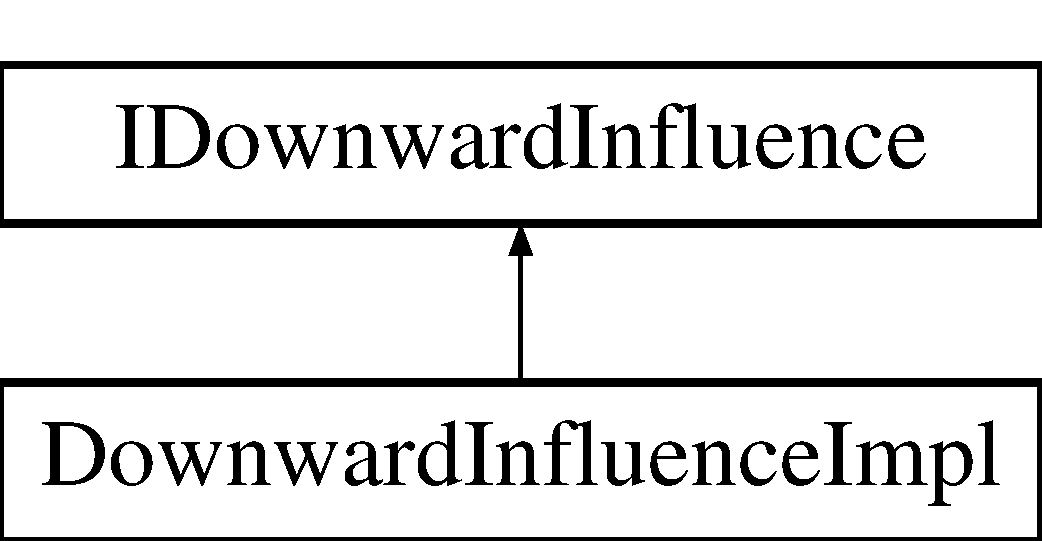
\includegraphics[height=2.000000cm]{classIDownwardInfluence}
\end{center}
\end{figure}
\subsection*{Public Member Functions}
\begin{DoxyCompactItemize}
\item 
{\bfseries I\+Downward\+Influence} (\hyperlink{classNode}{Node} $\ast$node)\hypertarget{classIDownwardInfluence_a7d5d6eb85ad3628703de8792dcebb9b5}{}\label{classIDownwardInfluence_a7d5d6eb85ad3628703de8792dcebb9b5}

\item 
virtual void {\bfseries calculate\+Downward\+Influence} ()=0\hypertarget{classIDownwardInfluence_ae6810945efb7ceb9b6e351c62bacd453}{}\label{classIDownwardInfluence_ae6810945efb7ceb9b6e351c62bacd453}

\end{DoxyCompactItemize}
\subsection*{Protected Attributes}
\begin{DoxyCompactItemize}
\item 
\hyperlink{classNode}{Node} $\ast$ {\bfseries m\+Node}\hypertarget{classIDownwardInfluence_aad871e67e020cdc589deb3739f8548a0}{}\label{classIDownwardInfluence_aad871e67e020cdc589deb3739f8548a0}

\end{DoxyCompactItemize}


The documentation for this class was generated from the following file\+:\begin{DoxyCompactItemize}
\item 
/home/mate/\+Documents/\+Programming/\+Research/\+Multilayer\+Network\+Model/\+Multilayer\+Network\+Model/src/core/include/I\+Downward\+Influence.\+hh\end{DoxyCompactItemize}

\hypertarget{classIDynamicalEquationGenerator}{}\section{I\+Dynamical\+Equation\+Generator Class Reference}
\label{classIDynamicalEquationGenerator}\index{I\+Dynamical\+Equation\+Generator@{I\+Dynamical\+Equation\+Generator}}
Inheritance diagram for I\+Dynamical\+Equation\+Generator\+:\begin{figure}[H]
\begin{center}
\leavevmode
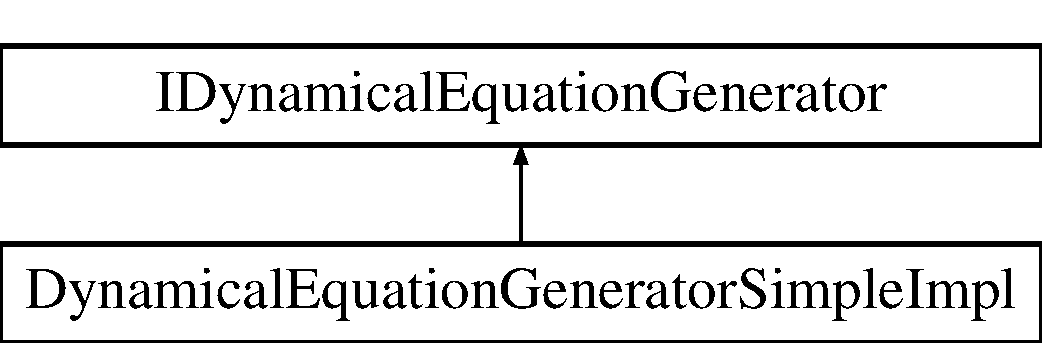
\includegraphics[height=2.000000cm]{classIDynamicalEquationGenerator}
\end{center}
\end{figure}
\subsection*{Public Member Functions}
\begin{DoxyCompactItemize}
\item 
{\bfseries I\+Dynamical\+Equation\+Generator} (\hyperlink{classMultilayerNetwork}{Multilayer\+Network} $\ast$multilayer\+Network)\hypertarget{classIDynamicalEquationGenerator_a7c4ee27a9153c6c71c56363509e9db50}{}\label{classIDynamicalEquationGenerator_a7c4ee27a9153c6c71c56363509e9db50}

\item 
virtual void {\bfseries generate\+Dynamical\+Equations} ()=0\hypertarget{classIDynamicalEquationGenerator_a23867fb164b2e17a98f2acde2f6d658e}{}\label{classIDynamicalEquationGenerator_a23867fb164b2e17a98f2acde2f6d658e}

\end{DoxyCompactItemize}
\subsection*{Protected Attributes}
\begin{DoxyCompactItemize}
\item 
\hyperlink{classMultilayerNetwork}{Multilayer\+Network} $\ast$ {\bfseries m\+Multilayer\+Network}\hypertarget{classIDynamicalEquationGenerator_aa20ebd4982dc045c28dba4e0fb63c585}{}\label{classIDynamicalEquationGenerator_aa20ebd4982dc045c28dba4e0fb63c585}

\end{DoxyCompactItemize}


The documentation for this class was generated from the following file\+:\begin{DoxyCompactItemize}
\item 
/home/mate/\+Documents/\+Programming/\+Research/\+Multilayer\+Network\+Model/\+Multilayer\+Network\+Model/sources/generators/include/I\+Dynamical\+Equation\+Generator.\+hh\end{DoxyCompactItemize}

\hypertarget{classIGenericRemoteSchemaDocumentProvider}{}\section{I\+Generic\+Remote\+Schema\+Document\+Provider$<$ Schema\+Document\+Type $>$ Class Template Reference}
\label{classIGenericRemoteSchemaDocumentProvider}\index{I\+Generic\+Remote\+Schema\+Document\+Provider$<$ Schema\+Document\+Type $>$@{I\+Generic\+Remote\+Schema\+Document\+Provider$<$ Schema\+Document\+Type $>$}}
\subsection*{Public Types}
\begin{DoxyCompactItemize}
\item 
typedef Schema\+Document\+Type\+::\+Ch {\bfseries Ch}\hypertarget{classIGenericRemoteSchemaDocumentProvider_acfcd5492c3df8ff56cd2d84d36cc0ceb}{}\label{classIGenericRemoteSchemaDocumentProvider_acfcd5492c3df8ff56cd2d84d36cc0ceb}

\end{DoxyCompactItemize}
\subsection*{Public Member Functions}
\begin{DoxyCompactItemize}
\item 
virtual const Schema\+Document\+Type $\ast$ {\bfseries Get\+Remote\+Document} (const Ch $\ast$uri, \hyperlink{rapidjson_8h_a5ed6e6e67250fadbd041127e6386dcb5}{Size\+Type} length)=0\hypertarget{classIGenericRemoteSchemaDocumentProvider_aad112a069dd57fe850fafd04cbb4777b}{}\label{classIGenericRemoteSchemaDocumentProvider_aad112a069dd57fe850fafd04cbb4777b}

\end{DoxyCompactItemize}


The documentation for this class was generated from the following files\+:\begin{DoxyCompactItemize}
\item 
/home/mate/\+Documents/\+Programming/\+Research/\+Multilayer\+Network\+Model/\+Multilayer\+Network\+Model/src/external/rapidjson/fwd.\+h\item 
/home/mate/\+Documents/\+Programming/\+Research/\+Multilayer\+Network\+Model/\+Multilayer\+Network\+Model/src/external/rapidjson/schema.\+h\end{DoxyCompactItemize}

\hypertarget{classIInitialConditionGenerator}{}\section{I\+Initial\+Condition\+Generator Class Reference}
\label{classIInitialConditionGenerator}\index{I\+Initial\+Condition\+Generator@{I\+Initial\+Condition\+Generator}}
Inheritance diagram for I\+Initial\+Condition\+Generator\+:\begin{figure}[H]
\begin{center}
\leavevmode
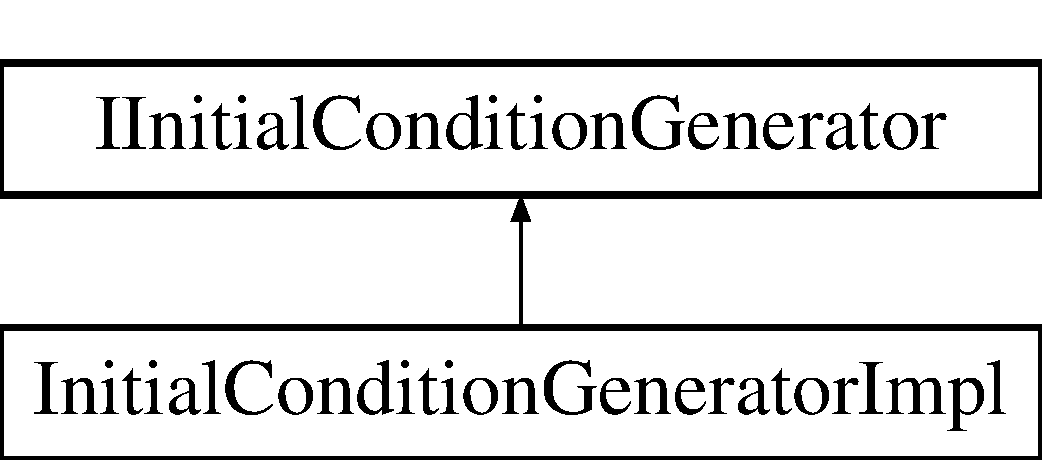
\includegraphics[height=2.000000cm]{classIInitialConditionGenerator}
\end{center}
\end{figure}
\subsection*{Public Member Functions}
\begin{DoxyCompactItemize}
\item 
{\bfseries I\+Initial\+Condition\+Generator} (\hyperlink{classMultilayerNetwork}{Multilayer\+Network} $\ast$multilayer\+Network)\hypertarget{classIInitialConditionGenerator_a23bef59a851914a65f67c2bd7736ad37}{}\label{classIInitialConditionGenerator_a23bef59a851914a65f67c2bd7736ad37}

\item 
virtual void {\bfseries generate\+Initial\+Condition} ()=0\hypertarget{classIInitialConditionGenerator_aaee78296548634e00150023baa051e52}{}\label{classIInitialConditionGenerator_aaee78296548634e00150023baa051e52}

\end{DoxyCompactItemize}
\subsection*{Protected Attributes}
\begin{DoxyCompactItemize}
\item 
\hyperlink{classMultilayerNetwork}{Multilayer\+Network} $\ast$ {\bfseries m\+Multilayer\+Network}\hypertarget{classIInitialConditionGenerator_a7144fdc9973103d6b377958868b4b387}{}\label{classIInitialConditionGenerator_a7144fdc9973103d6b377958868b4b387}

\end{DoxyCompactItemize}


The documentation for this class was generated from the following file\+:\begin{DoxyCompactItemize}
\item 
/home/mate/\+Documents/\+Programming/\+Research/\+Multilayer\+Network\+Model/\+Multilayer\+Network\+Model/src/generators/include/I\+Initial\+Condition\+Generator.\+hh\end{DoxyCompactItemize}

\hypertarget{structimaxdiv__t}{}\section{imaxdiv\+\_\+t Struct Reference}
\label{structimaxdiv__t}\index{imaxdiv\+\_\+t@{imaxdiv\+\_\+t}}
\subsection*{Public Attributes}
\begin{DoxyCompactItemize}
\item 
intmax\+\_\+t {\bfseries quot}\hypertarget{structimaxdiv__t_a9339814cbb7610c72fb7d30c6573b393}{}\label{structimaxdiv__t_a9339814cbb7610c72fb7d30c6573b393}

\item 
intmax\+\_\+t {\bfseries rem}\hypertarget{structimaxdiv__t_a6c9701ad10bff81edae7ff679cae7850}{}\label{structimaxdiv__t_a6c9701ad10bff81edae7ff679cae7850}

\end{DoxyCompactItemize}


The documentation for this struct was generated from the following file\+:\begin{DoxyCompactItemize}
\item 
/home/mate/\+Documents/\+Programming/\+Research/\+Multilayer\+Network\+Model/\+Multilayer\+Network\+Model/sources/external/rapidjson/msinttypes/inttypes.\+h\end{DoxyCompactItemize}

\hypertarget{classInitialConditionGeneratorImpl}{}\section{Initial\+Condition\+Generator\+Impl Class Reference}
\label{classInitialConditionGeneratorImpl}\index{Initial\+Condition\+Generator\+Impl@{Initial\+Condition\+Generator\+Impl}}
Inheritance diagram for Initial\+Condition\+Generator\+Impl\+:\begin{figure}[H]
\begin{center}
\leavevmode
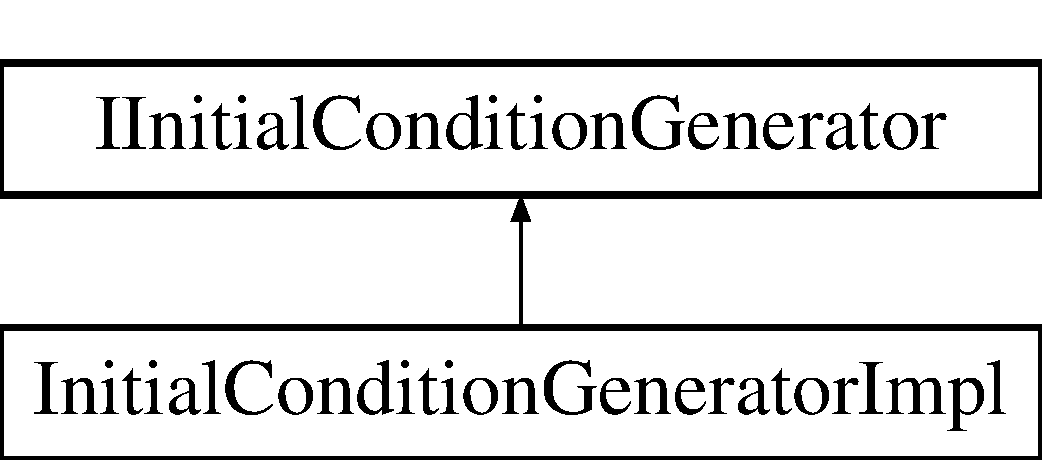
\includegraphics[height=2.000000cm]{classInitialConditionGeneratorImpl}
\end{center}
\end{figure}
\subsection*{Public Member Functions}
\begin{DoxyCompactItemize}
\item 
{\bfseries Initial\+Condition\+Generator\+Impl} (\hyperlink{classMultilayerNetwork}{Multilayer\+Network} $\ast$multilayer\+Network)\hypertarget{classInitialConditionGeneratorImpl_a07647da5a3eece4804a53135bb54c738}{}\label{classInitialConditionGeneratorImpl_a07647da5a3eece4804a53135bb54c738}

\item 
void {\bfseries generate\+Initial\+Condition} ()\hypertarget{classInitialConditionGeneratorImpl_ab296cde00693ad9b2b0199c69a3c3326}{}\label{classInitialConditionGeneratorImpl_ab296cde00693ad9b2b0199c69a3c3326}

\end{DoxyCompactItemize}
\subsection*{Additional Inherited Members}


The documentation for this class was generated from the following files\+:\begin{DoxyCompactItemize}
\item 
/home/mate/\+Documents/\+Programming/\+Research/\+Multilayer\+Network\+Model/\+Multilayer\+Network\+Model/sources/generators/include/Initial\+Condition\+Generator\+Impl.\+hh\item 
/home/mate/\+Documents/\+Programming/\+Research/\+Multilayer\+Network\+Model/\+Multilayer\+Network\+Model/sources/generators/src/Initial\+Condition\+Generator\+Impl.\+cc\end{DoxyCompactItemize}

\hypertarget{classEquationParser_1_1Interpreter}{}\section{Equation\+Parser\+:\+:Interpreter Class Reference}
\label{classEquationParser_1_1Interpreter}\index{Equation\+Parser\+::\+Interpreter@{Equation\+Parser\+::\+Interpreter}}
\subsection*{Public Member Functions}
\begin{DoxyCompactItemize}
\item 
int {\bfseries parse} ()\hypertarget{classEquationParser_1_1Interpreter_aa88f207642eaa0a2d04cf5d050957c1a}{}\label{classEquationParser_1_1Interpreter_aa88f207642eaa0a2d04cf5d050957c1a}

\item 
\hyperlink{classCalculationNode}{Calculation\+Node} $\ast$ {\bfseries get\+Base\+Calculation\+Node} ()\hypertarget{classEquationParser_1_1Interpreter_ac861c17080e13412300574e96612d114}{}\label{classEquationParser_1_1Interpreter_ac861c17080e13412300574e96612d114}

\item 
void {\bfseries switch\+Input\+Stream} (std\+::istringstream $\ast$is)\hypertarget{classEquationParser_1_1Interpreter_a4dc3765926d0bf9d103859f713bd1e32}{}\label{classEquationParser_1_1Interpreter_a4dc3765926d0bf9d103859f713bd1e32}

\item 
void {\bfseries print\+Calculation\+Nodes} ()\hypertarget{classEquationParser_1_1Interpreter_a0281f87ae26693913d9b880efb3cc525}{}\label{classEquationParser_1_1Interpreter_a0281f87ae26693913d9b880efb3cc525}

\end{DoxyCompactItemize}
\subsection*{Friends}
\begin{DoxyCompactItemize}
\item 
class {\bfseries Parser}\hypertarget{classEquationParser_1_1Interpreter_ab80291af9c262f63b83fa9c16f12014d}{}\label{classEquationParser_1_1Interpreter_ab80291af9c262f63b83fa9c16f12014d}

\item 
class {\bfseries Scanner}\hypertarget{classEquationParser_1_1Interpreter_af4a8f36320cb35fb6b88d6b9a33cb524}{}\label{classEquationParser_1_1Interpreter_af4a8f36320cb35fb6b88d6b9a33cb524}

\end{DoxyCompactItemize}


The documentation for this class was generated from the following files\+:\begin{DoxyCompactItemize}
\item 
/home/mate/\+Documents/\+Programming/\+Research/\+Multilayer\+Network\+Model/\+Multilayer\+Network\+Model/sources/parser/include/interpreter.\+h\item 
/home/mate/\+Documents/\+Programming/\+Research/\+Multilayer\+Network\+Model/\+Multilayer\+Network\+Model/sources/parser/src/interpreter.\+cpp\end{DoxyCompactItemize}

\hypertarget{classinternal_1_1ISchemaStateFactory}{}\section{internal\+:\+:I\+Schema\+State\+Factory$<$ Schema\+Type $>$ Class Template Reference}
\label{classinternal_1_1ISchemaStateFactory}\index{internal\+::\+I\+Schema\+State\+Factory$<$ Schema\+Type $>$@{internal\+::\+I\+Schema\+State\+Factory$<$ Schema\+Type $>$}}
\subsection*{Public Member Functions}
\begin{DoxyCompactItemize}
\item 
virtual \hyperlink{classinternal_1_1ISchemaValidator}{I\+Schema\+Validator} $\ast$ {\bfseries Create\+Schema\+Validator} (const Schema\+Type \&)=0\hypertarget{classinternal_1_1ISchemaStateFactory_ae8c98fcff6a057b4fcd9018fc14551a8}{}\label{classinternal_1_1ISchemaStateFactory_ae8c98fcff6a057b4fcd9018fc14551a8}

\item 
virtual void {\bfseries Destroy\+Schema\+Validator} (\hyperlink{classinternal_1_1ISchemaValidator}{I\+Schema\+Validator} $\ast$validator)=0\hypertarget{classinternal_1_1ISchemaStateFactory_a112cbf154077050bc30ffe670032442c}{}\label{classinternal_1_1ISchemaStateFactory_a112cbf154077050bc30ffe670032442c}

\item 
virtual void $\ast$ {\bfseries Create\+Hasher} ()=0\hypertarget{classinternal_1_1ISchemaStateFactory_a4ac37b9d3e9526004c82692473f978f4}{}\label{classinternal_1_1ISchemaStateFactory_a4ac37b9d3e9526004c82692473f978f4}

\item 
virtual uint64\+\_\+t {\bfseries Get\+Hash\+Code} (void $\ast$hasher)=0\hypertarget{classinternal_1_1ISchemaStateFactory_addfcf00963cc777edf642b204f07c8d6}{}\label{classinternal_1_1ISchemaStateFactory_addfcf00963cc777edf642b204f07c8d6}

\item 
virtual void {\bfseries Destrory\+Hasher} (void $\ast$hasher)=0\hypertarget{classinternal_1_1ISchemaStateFactory_a70b8d88180d2e6993105b17f19101635}{}\label{classinternal_1_1ISchemaStateFactory_a70b8d88180d2e6993105b17f19101635}

\item 
virtual void $\ast$ {\bfseries Malloc\+State} (size\+\_\+t size)=0\hypertarget{classinternal_1_1ISchemaStateFactory_ada92ebf8e9ef994f7e20a0f7f9750519}{}\label{classinternal_1_1ISchemaStateFactory_ada92ebf8e9ef994f7e20a0f7f9750519}

\item 
virtual void {\bfseries Free\+State} (void $\ast$p)=0\hypertarget{classinternal_1_1ISchemaStateFactory_a27bd2138940cac3c330dd8399c49b22b}{}\label{classinternal_1_1ISchemaStateFactory_a27bd2138940cac3c330dd8399c49b22b}

\end{DoxyCompactItemize}


The documentation for this class was generated from the following file\+:\begin{DoxyCompactItemize}
\item 
/home/mate/\+Documents/\+Programming/\+Research/\+Multilayer\+Network\+Model/\+Multilayer\+Network\+Model/src/external/rapidjson/schema.\+h\end{DoxyCompactItemize}

\hypertarget{classinternal_1_1ISchemaValidator}{}\section{internal\+:\+:I\+Schema\+Validator Class Reference}
\label{classinternal_1_1ISchemaValidator}\index{internal\+::\+I\+Schema\+Validator@{internal\+::\+I\+Schema\+Validator}}
Inheritance diagram for internal\+:\+:I\+Schema\+Validator\+:\begin{figure}[H]
\begin{center}
\leavevmode
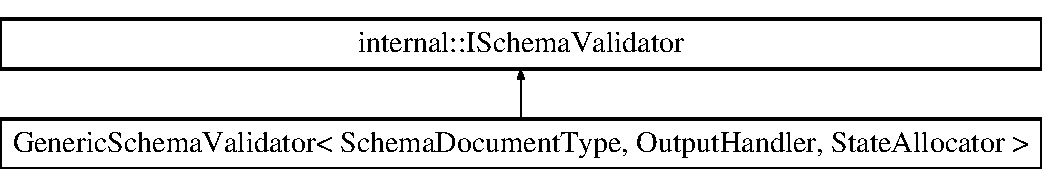
\includegraphics[height=2.000000cm]{classinternal_1_1ISchemaValidator}
\end{center}
\end{figure}
\subsection*{Public Member Functions}
\begin{DoxyCompactItemize}
\item 
virtual bool {\bfseries Is\+Valid} () const  =0\hypertarget{classinternal_1_1ISchemaValidator_ad9c95f664966bec385dbe85f33a6ba3d}{}\label{classinternal_1_1ISchemaValidator_ad9c95f664966bec385dbe85f33a6ba3d}

\end{DoxyCompactItemize}


The documentation for this class was generated from the following file\+:\begin{DoxyCompactItemize}
\item 
/home/mate/\+Documents/\+Programming/\+Research/\+Multilayer\+Network\+Model/\+Multilayer\+Network\+Model/src/external/rapidjson/schema.\+h\end{DoxyCompactItemize}

\hypertarget{structinternal_1_1IsGenericValue}{}\section{internal\+:\+:Is\+Generic\+Value$<$ T $>$ Struct Template Reference}
\label{structinternal_1_1IsGenericValue}\index{internal\+::\+Is\+Generic\+Value$<$ T $>$@{internal\+::\+Is\+Generic\+Value$<$ T $>$}}
Inheritance diagram for internal\+:\+:Is\+Generic\+Value$<$ T $>$\+:\begin{figure}[H]
\begin{center}
\leavevmode
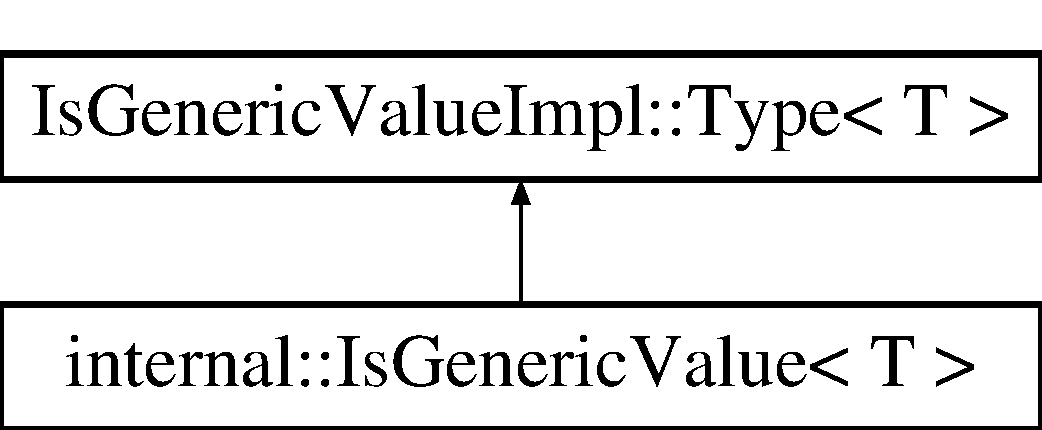
\includegraphics[height=2.000000cm]{structinternal_1_1IsGenericValue}
\end{center}
\end{figure}


The documentation for this struct was generated from the following file\+:\begin{DoxyCompactItemize}
\item 
/home/mate/\+Documents/\+Programming/\+Research/\+Multilayer\+Network\+Model/\+Multilayer\+Network\+Model/src/external/rapidjson/\hyperlink{document_8h}{document.\+h}\end{DoxyCompactItemize}

\hypertarget{structinternal_1_1IsGenericValueImpl}{}\section{internal\+:\+:Is\+Generic\+Value\+Impl$<$ T, Encoding, Allocator $>$ Struct Template Reference}
\label{structinternal_1_1IsGenericValueImpl}\index{internal\+::\+Is\+Generic\+Value\+Impl$<$ T, Encoding, Allocator $>$@{internal\+::\+Is\+Generic\+Value\+Impl$<$ T, Encoding, Allocator $>$}}
Inheritance diagram for internal\+:\+:Is\+Generic\+Value\+Impl$<$ T, Encoding, Allocator $>$\+:\begin{figure}[H]
\begin{center}
\leavevmode
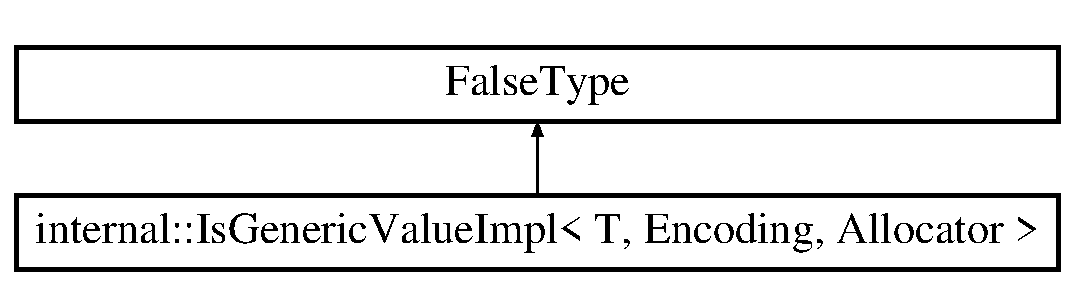
\includegraphics[height=2.000000cm]{structinternal_1_1IsGenericValueImpl}
\end{center}
\end{figure}


The documentation for this struct was generated from the following file\+:\begin{DoxyCompactItemize}
\item 
/home/mate/\+Documents/\+Programming/\+Research/\+Multilayer\+Network\+Model/\+Multilayer\+Network\+Model/src/external/rapidjson/\hyperlink{document_8h}{document.\+h}\end{DoxyCompactItemize}

\hypertarget{structinternal_1_1IsGenericValueImpl_3_01T_00_01typename_01Void_3_01typename_01T_1_1EncodingType794abcc01fcce01e300668fa57e4d036}{}\section{internal\+:\+:Is\+Generic\+Value\+Impl$<$ T, typename Void$<$ typename T\+:\+:Encoding\+Type $>$\+:\+:Type, typename Void$<$ typename T\+:\+:Allocator\+Type $>$\+:\+:Type $>$ Struct Template Reference}
\label{structinternal_1_1IsGenericValueImpl_3_01T_00_01typename_01Void_3_01typename_01T_1_1EncodingType794abcc01fcce01e300668fa57e4d036}\index{internal\+::\+Is\+Generic\+Value\+Impl$<$ T, typename Void$<$ typename T\+::\+Encoding\+Type $>$\+::\+Type, typename Void$<$ typename T\+::\+Allocator\+Type $>$\+::\+Type $>$@{internal\+::\+Is\+Generic\+Value\+Impl$<$ T, typename Void$<$ typename T\+::\+Encoding\+Type $>$\+::\+Type, typename Void$<$ typename T\+::\+Allocator\+Type $>$\+::\+Type $>$}}
Inheritance diagram for internal\+:\+:Is\+Generic\+Value\+Impl$<$ T, typename Void$<$ typename T\+:\+:Encoding\+Type $>$\+:\+:Type, typename Void$<$ typename T\+:\+:Allocator\+Type $>$\+:\+:Type $>$\+:\begin{figure}[H]
\begin{center}
\leavevmode
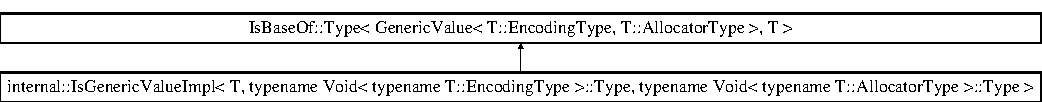
\includegraphics[height=1.372549cm]{structinternal_1_1IsGenericValueImpl_3_01T_00_01typename_01Void_3_01typename_01T_1_1EncodingType794abcc01fcce01e300668fa57e4d036}
\end{center}
\end{figure}


The documentation for this struct was generated from the following file\+:\begin{DoxyCompactItemize}
\item 
/home/mate/\+Documents/\+Programming/\+Research/\+Multilayer\+Network\+Model/\+Multilayer\+Network\+Model/sources/external/rapidjson/\hyperlink{document_8h}{document.\+h}\end{DoxyCompactItemize}

\hypertarget{classIStructureGenerator}{}\section{I\+Structure\+Generator Class Reference}
\label{classIStructureGenerator}\index{I\+Structure\+Generator@{I\+Structure\+Generator}}
Inheritance diagram for I\+Structure\+Generator\+:\begin{figure}[H]
\begin{center}
\leavevmode
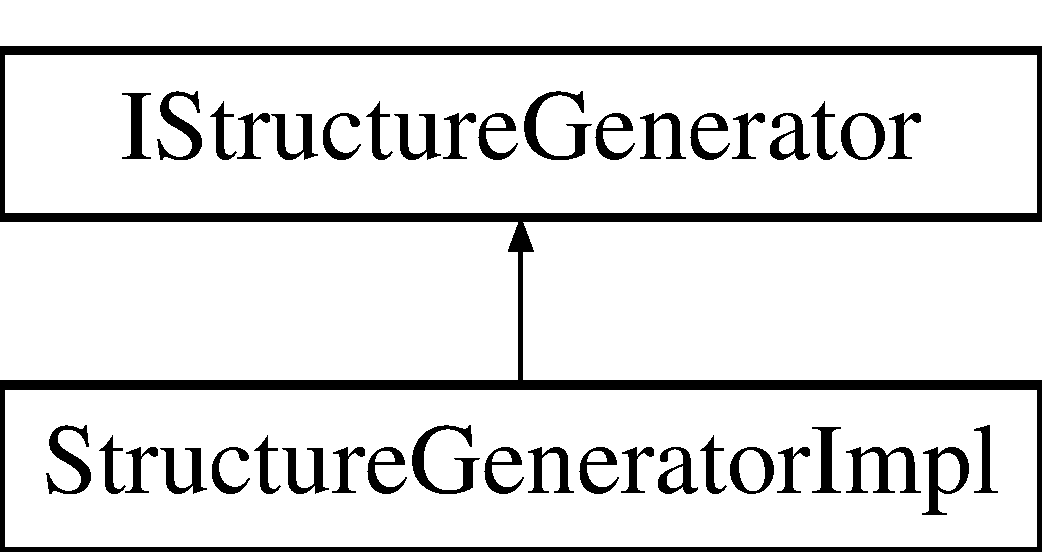
\includegraphics[height=2.000000cm]{classIStructureGenerator}
\end{center}
\end{figure}
\subsection*{Public Member Functions}
\begin{DoxyCompactItemize}
\item 
{\bfseries I\+Structure\+Generator} (\hyperlink{classMultilayerNetwork}{Multilayer\+Network} $\ast$multilayer\+Network)\hypertarget{classIStructureGenerator_af1536f217b3898a794a23417b3a0a2ed}{}\label{classIStructureGenerator_af1536f217b3898a794a23417b3a0a2ed}

\item 
virtual void {\bfseries generate\+Structure} ()=0\hypertarget{classIStructureGenerator_a6fd7b5ad3b544e5069e83a5fc62e249c}{}\label{classIStructureGenerator_a6fd7b5ad3b544e5069e83a5fc62e249c}

\end{DoxyCompactItemize}
\subsection*{Protected Attributes}
\begin{DoxyCompactItemize}
\item 
\hyperlink{classMultilayerNetwork}{Multilayer\+Network} $\ast$ {\bfseries m\+Multilayer\+Network}\hypertarget{classIStructureGenerator_af3bd39449b5256b4e4505005c34f33c4}{}\label{classIStructureGenerator_af3bd39449b5256b4e4505005c34f33c4}

\end{DoxyCompactItemize}


The documentation for this class was generated from the following file\+:\begin{DoxyCompactItemize}
\item 
/home/mate/\+Documents/\+Programming/\+Research/\+Multilayer\+Network\+Model/\+Multilayer\+Network\+Model/sources/generators/include/I\+Structure\+Generator.\+hh\end{DoxyCompactItemize}

\hypertarget{classIUpwardInfluence}{}\section{I\+Upward\+Influence Class Reference}
\label{classIUpwardInfluence}\index{I\+Upward\+Influence@{I\+Upward\+Influence}}
Inheritance diagram for I\+Upward\+Influence\+:\begin{figure}[H]
\begin{center}
\leavevmode
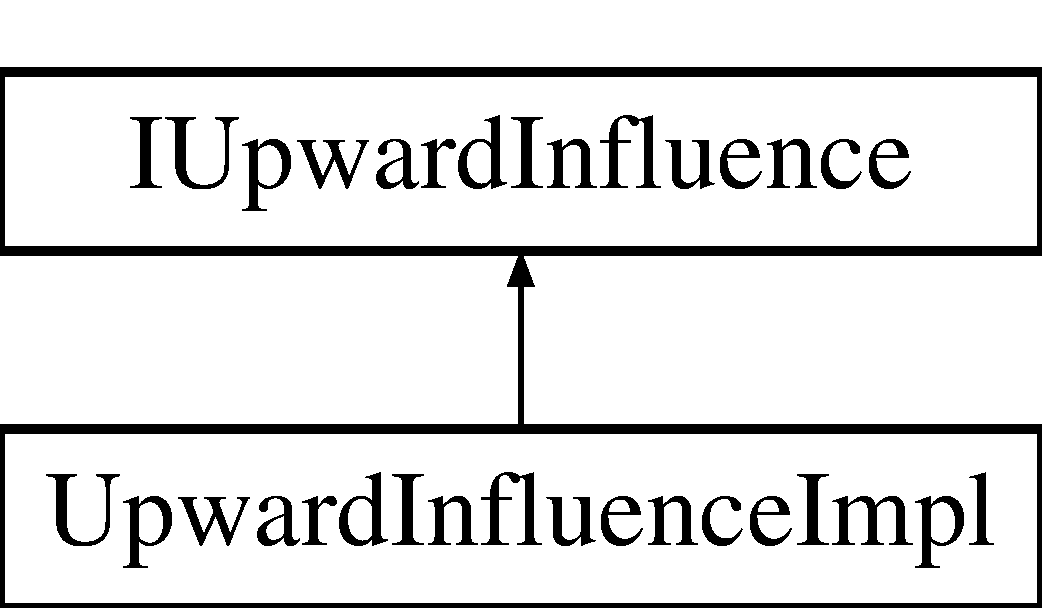
\includegraphics[height=2.000000cm]{classIUpwardInfluence}
\end{center}
\end{figure}
\subsection*{Public Member Functions}
\begin{DoxyCompactItemize}
\item 
{\bfseries I\+Upward\+Influence} (\hyperlink{classNode}{Node} $\ast$node)\hypertarget{classIUpwardInfluence_adc85bc94bdd2b99e474db59901e1cc7b}{}\label{classIUpwardInfluence_adc85bc94bdd2b99e474db59901e1cc7b}

\item 
virtual void {\bfseries calculate\+Upward\+Influence} ()=0\hypertarget{classIUpwardInfluence_adcb9517abfc35398e212fd47af22fdb0}{}\label{classIUpwardInfluence_adcb9517abfc35398e212fd47af22fdb0}

\end{DoxyCompactItemize}
\subsection*{Protected Attributes}
\begin{DoxyCompactItemize}
\item 
\hyperlink{classNode}{Node} $\ast$ {\bfseries m\+Node}\hypertarget{classIUpwardInfluence_aba560a3989e018d2526b14ad91d52ea4}{}\label{classIUpwardInfluence_aba560a3989e018d2526b14ad91d52ea4}

\end{DoxyCompactItemize}


The documentation for this class was generated from the following file\+:\begin{DoxyCompactItemize}
\item 
/home/mate/\+Documents/\+Programming/\+Research/\+Multilayer\+Network\+Model/\+Multilayer\+Network\+Model/src/core/include/I\+Upward\+Influence.\+hh\end{DoxyCompactItemize}

\hypertarget{classIVectorFieldReconfiguration}{}\section{I\+Vector\+Field\+Reconfiguration Class Reference}
\label{classIVectorFieldReconfiguration}\index{I\+Vector\+Field\+Reconfiguration@{I\+Vector\+Field\+Reconfiguration}}
Inheritance diagram for I\+Vector\+Field\+Reconfiguration\+:\begin{figure}[H]
\begin{center}
\leavevmode
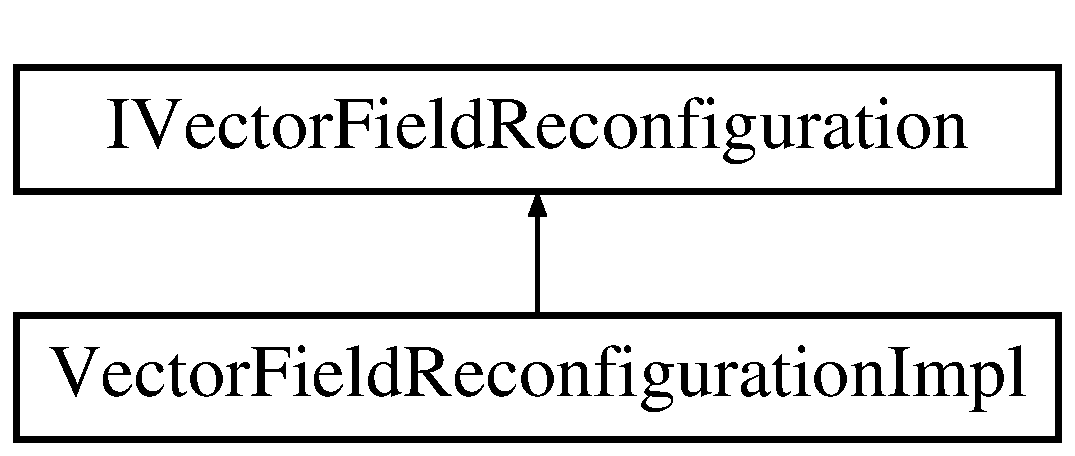
\includegraphics[height=2.000000cm]{classIVectorFieldReconfiguration}
\end{center}
\end{figure}
\subsection*{Public Member Functions}
\begin{DoxyCompactItemize}
\item 
{\bfseries I\+Vector\+Field\+Reconfiguration} (\hyperlink{classNode}{Node} $\ast$node)\hypertarget{classIVectorFieldReconfiguration_a6b663421658c873129a81c3597e0a4c1}{}\label{classIVectorFieldReconfiguration_a6b663421658c873129a81c3597e0a4c1}

\item 
virtual void {\bfseries calculate\+Vector\+Field\+Reconfiguration} ()=0\hypertarget{classIVectorFieldReconfiguration_a3d4ae2c51645c6e6e1955d7ea152ec04}{}\label{classIVectorFieldReconfiguration_a3d4ae2c51645c6e6e1955d7ea152ec04}

\end{DoxyCompactItemize}
\subsection*{Protected Attributes}
\begin{DoxyCompactItemize}
\item 
\hyperlink{classNode}{Node} $\ast$ {\bfseries m\+Node}\hypertarget{classIVectorFieldReconfiguration_a3a8452d0f63f8c9e05e1ad6faab26325}{}\label{classIVectorFieldReconfiguration_a3a8452d0f63f8c9e05e1ad6faab26325}

\end{DoxyCompactItemize}


The documentation for this class was generated from the following file\+:\begin{DoxyCompactItemize}
\item 
/home/mate/\+Documents/\+Programming/\+Research/\+Multilayer\+Network\+Model/\+Multilayer\+Network\+Model/src/core/include/I\+Vector\+Field\+Reconfiguration.\+hh\end{DoxyCompactItemize}

\hypertarget{classLayer}{}\section{Layer Class Reference}
\label{classLayer}\index{Layer@{Layer}}
\subsection*{Public Member Functions}
\begin{DoxyCompactItemize}
\item 
{\bfseries Layer} (int)\hypertarget{classLayer_a3f0552558b7008ebe37b74d55181d2a8}{}\label{classLayer_a3f0552558b7008ebe37b74d55181d2a8}

\item 
void {\bfseries add\+Network} (int network\+Id)\hypertarget{classLayer_ae76589e097e0fc8d3fc0d16c83670a5c}{}\label{classLayer_ae76589e097e0fc8d3fc0d16c83670a5c}

\item 
std\+::vector$<$ \hyperlink{classNetwork}{Network} $\ast$ $>$ {\bfseries get\+Networks} (void) const \hypertarget{classLayer_a7c8fe4f0a91522c0ffbb4b6ed3d507f1}{}\label{classLayer_a7c8fe4f0a91522c0ffbb4b6ed3d507f1}

\item 
int {\bfseries get\+Id} (void) const \hypertarget{classLayer_a00123131915f8bef4bf58bda3229e80c}{}\label{classLayer_a00123131915f8bef4bf58bda3229e80c}

\end{DoxyCompactItemize}
\subsection*{Friends}
\begin{DoxyCompactItemize}
\item 
bool {\bfseries operator==} (const \hyperlink{classLayer}{Layer} \&layer1, const \hyperlink{classLayer}{Layer} \&layer2)\hypertarget{classLayer_aca6ebc1f2e29896977fd9434db21761b}{}\label{classLayer_aca6ebc1f2e29896977fd9434db21761b}

\end{DoxyCompactItemize}


The documentation for this class was generated from the following files\+:\begin{DoxyCompactItemize}
\item 
/home/mate/\+Documents/\+Programming/\+Research/\+Multilayer\+Network\+Model/\+Multilayer\+Network\+Model/src/core/include/Layer.\+hh\item 
/home/mate/\+Documents/\+Programming/\+Research/\+Multilayer\+Network\+Model/\+Multilayer\+Network\+Model/src/core/src/Layer.\+cc\end{DoxyCompactItemize}

\hypertarget{structWriter_1_1Level}{}\section{Writer$<$ Output\+Stream, Source\+Encoding, Target\+Encoding, Stack\+Allocator, write\+Flags $>$\+:\+:Level Struct Reference}
\label{structWriter_1_1Level}\index{Writer$<$ Output\+Stream, Source\+Encoding, Target\+Encoding, Stack\+Allocator, write\+Flags $>$\+::\+Level@{Writer$<$ Output\+Stream, Source\+Encoding, Target\+Encoding, Stack\+Allocator, write\+Flags $>$\+::\+Level}}


Information for each nested level.  




{\ttfamily \#include $<$writer.\+h$>$}

\subsection*{Public Member Functions}
\begin{DoxyCompactItemize}
\item 
{\bfseries Level} (bool in\+Array\+\_\+)\hypertarget{structWriter_1_1Level_a0b1844a7a1b7c6c20e1964dbb67da484}{}\label{structWriter_1_1Level_a0b1844a7a1b7c6c20e1964dbb67da484}

\end{DoxyCompactItemize}
\subsection*{Public Attributes}
\begin{DoxyCompactItemize}
\item 
size\+\_\+t \hyperlink{structWriter_1_1Level_a4a09e5fda49d0d57b2adc041203f244f}{value\+Count}\hypertarget{structWriter_1_1Level_a4a09e5fda49d0d57b2adc041203f244f}{}\label{structWriter_1_1Level_a4a09e5fda49d0d57b2adc041203f244f}

\begin{DoxyCompactList}\small\item\em number of values in this level \end{DoxyCompactList}\item 
bool \hyperlink{structWriter_1_1Level_aa009a2d675e98757c2997072aad78789}{in\+Array}\hypertarget{structWriter_1_1Level_aa009a2d675e98757c2997072aad78789}{}\label{structWriter_1_1Level_aa009a2d675e98757c2997072aad78789}

\begin{DoxyCompactList}\small\item\em true if in array, otherwise in object \end{DoxyCompactList}\end{DoxyCompactItemize}


\subsection{Detailed Description}
\subsubsection*{template$<$typename Output\+Stream, typename Source\+Encoding = U\+T\+F8$<$$>$, typename Target\+Encoding = U\+T\+F8$<$$>$, typename Stack\+Allocator = Crt\+Allocator, unsigned write\+Flags = k\+Write\+Default\+Flags$>$\\*
struct Writer$<$ Output\+Stream, Source\+Encoding, Target\+Encoding, Stack\+Allocator, write\+Flags $>$\+::\+Level}

Information for each nested level. 

The documentation for this struct was generated from the following file\+:\begin{DoxyCompactItemize}
\item 
/home/mate/\+Documents/\+Programming/\+Research/\+Multilayer\+Network\+Model/\+Multilayer\+Network\+Model/sources/external/rapidjson/writer.\+h\end{DoxyCompactItemize}

\hypertarget{classEquationParser_1_1location}{}\section{Equation\+Parser\+:\+:location Class Reference}
\label{classEquationParser_1_1location}\index{Equation\+Parser\+::location@{Equation\+Parser\+::location}}


Abstract a location.  




{\ttfamily \#include $<$location.\+hh$>$}

\subsection*{Public Member Functions}
\begin{DoxyCompactItemize}
\item 
\hyperlink{classEquationParser_1_1location_a92b5f6e32ea3eabe14f537698b9f4563}{location} (const \hyperlink{classEquationParser_1_1position}{position} \&b, const \hyperlink{classEquationParser_1_1position}{position} \&e)\hypertarget{classEquationParser_1_1location_a92b5f6e32ea3eabe14f537698b9f4563}{}\label{classEquationParser_1_1location_a92b5f6e32ea3eabe14f537698b9f4563}

\begin{DoxyCompactList}\small\item\em Construct a location from {\itshape b} to {\itshape e}. \end{DoxyCompactList}\item 
\hyperlink{classEquationParser_1_1location_a461e436649b6fae8e2cde43e4140f8f3}{location} (const \hyperlink{classEquationParser_1_1position}{position} \&p=\hyperlink{classEquationParser_1_1position}{position}())\hypertarget{classEquationParser_1_1location_a461e436649b6fae8e2cde43e4140f8f3}{}\label{classEquationParser_1_1location_a461e436649b6fae8e2cde43e4140f8f3}

\begin{DoxyCompactList}\small\item\em Construct a 0-\/width location in {\itshape p}. \end{DoxyCompactList}\item 
\hyperlink{classEquationParser_1_1location_a00c520c87490f3dee70875782480256f}{location} (std\+::string $\ast$f, unsigned int l=1u, unsigned int c=1u)\hypertarget{classEquationParser_1_1location_a00c520c87490f3dee70875782480256f}{}\label{classEquationParser_1_1location_a00c520c87490f3dee70875782480256f}

\begin{DoxyCompactList}\small\item\em Construct a 0-\/width location in {\itshape f}, {\itshape l}, {\itshape c}. \end{DoxyCompactList}\item 
void \hyperlink{classEquationParser_1_1location_a5c7d7aa2ae28c40f506e83514acb3947}{initialize} (std\+::string $\ast$f=Y\+Y\+\_\+\+N\+U\+L\+L\+P\+TR, unsigned int l=1u, unsigned int c=1u)\hypertarget{classEquationParser_1_1location_a5c7d7aa2ae28c40f506e83514acb3947}{}\label{classEquationParser_1_1location_a5c7d7aa2ae28c40f506e83514acb3947}

\begin{DoxyCompactList}\small\item\em Initialization. \end{DoxyCompactList}\end{DoxyCompactItemize}
\begin{Indent}{\bf Line and Column related manipulators}\par
\begin{DoxyCompactItemize}
\item 
void \hyperlink{classEquationParser_1_1location_a8796256e64c782808b9e6cc5076f7b6b}{step} ()\hypertarget{classEquationParser_1_1location_a8796256e64c782808b9e6cc5076f7b6b}{}\label{classEquationParser_1_1location_a8796256e64c782808b9e6cc5076f7b6b}

\begin{DoxyCompactList}\small\item\em Reset initial location to final location. \end{DoxyCompactList}\item 
void \hyperlink{classEquationParser_1_1location_aef9d17fbbfb8a0a98cd0bf3356008a72}{columns} (int count=1)\hypertarget{classEquationParser_1_1location_aef9d17fbbfb8a0a98cd0bf3356008a72}{}\label{classEquationParser_1_1location_aef9d17fbbfb8a0a98cd0bf3356008a72}

\begin{DoxyCompactList}\small\item\em Extend the current location to the C\+O\+U\+NT next columns. \end{DoxyCompactList}\item 
void \hyperlink{classEquationParser_1_1location_a856b91626aa857984a450e4395a4f41c}{lines} (int count=1)\hypertarget{classEquationParser_1_1location_a856b91626aa857984a450e4395a4f41c}{}\label{classEquationParser_1_1location_a856b91626aa857984a450e4395a4f41c}

\begin{DoxyCompactList}\small\item\em Extend the current location to the C\+O\+U\+NT next lines. \end{DoxyCompactList}\end{DoxyCompactItemize}
\end{Indent}
\subsection*{Public Attributes}
\begin{DoxyCompactItemize}
\item 
\hyperlink{classEquationParser_1_1position}{position} \hyperlink{classEquationParser_1_1location_aa1fdd6decfaa33b12c14a71895c6c5cb}{begin}\hypertarget{classEquationParser_1_1location_aa1fdd6decfaa33b12c14a71895c6c5cb}{}\label{classEquationParser_1_1location_aa1fdd6decfaa33b12c14a71895c6c5cb}

\begin{DoxyCompactList}\small\item\em Beginning of the located region. \end{DoxyCompactList}\item 
\hyperlink{classEquationParser_1_1position}{position} \hyperlink{classEquationParser_1_1location_a6399485d967cdee3a129a748a2b385f7}{end}\hypertarget{classEquationParser_1_1location_a6399485d967cdee3a129a748a2b385f7}{}\label{classEquationParser_1_1location_a6399485d967cdee3a129a748a2b385f7}

\begin{DoxyCompactList}\small\item\em End of the located region. \end{DoxyCompactList}\end{DoxyCompactItemize}


\subsection{Detailed Description}
Abstract a location. 

The documentation for this class was generated from the following file\+:\begin{DoxyCompactItemize}
\item 
/home/mate/\+Documents/\+Programming/\+Research/\+Multilayer\+Network\+Model/\+Multilayer\+Network\+Model/src/parser/include/\hyperlink{location_8hh}{location.\+hh}\end{DoxyCompactItemize}

\hypertarget{classMemoryPoolAllocator}{}\section{Memory\+Pool\+Allocator$<$ Base\+Allocator $>$ Class Template Reference}
\label{classMemoryPoolAllocator}\index{Memory\+Pool\+Allocator$<$ Base\+Allocator $>$@{Memory\+Pool\+Allocator$<$ Base\+Allocator $>$}}


Default memory allocator used by the parser and D\+OM.  




{\ttfamily \#include $<$allocators.\+h$>$}

\subsection*{Public Member Functions}
\begin{DoxyCompactItemize}
\item 
\hyperlink{classMemoryPoolAllocator_aeec85ac657f242ac5620115141be5209}{Memory\+Pool\+Allocator} (size\+\_\+t chunk\+Size=k\+Default\+Chunk\+Capacity, Base\+Allocator $\ast$base\+Allocator=0)
\begin{DoxyCompactList}\small\item\em Constructor with chunk\+Size. \end{DoxyCompactList}\item 
\hyperlink{classMemoryPoolAllocator_a1f0d865093fdb955d956b7a445a8ddbf}{Memory\+Pool\+Allocator} (void $\ast$buffer, size\+\_\+t size, size\+\_\+t chunk\+Size=k\+Default\+Chunk\+Capacity, Base\+Allocator $\ast$base\+Allocator=0)
\begin{DoxyCompactList}\small\item\em Constructor with user-\/supplied buffer. \end{DoxyCompactList}\item 
\hyperlink{classMemoryPoolAllocator_ad4eee0ef3cfe8cda31034fbce98b7a9b}{$\sim$\+Memory\+Pool\+Allocator} ()
\begin{DoxyCompactList}\small\item\em Destructor. \end{DoxyCompactList}\item 
void \hyperlink{classMemoryPoolAllocator_a57bbc80e570db6110901b9a7e36dbda0}{Clear} ()\hypertarget{classMemoryPoolAllocator_a57bbc80e570db6110901b9a7e36dbda0}{}\label{classMemoryPoolAllocator_a57bbc80e570db6110901b9a7e36dbda0}

\begin{DoxyCompactList}\small\item\em Deallocates all memory chunks, excluding the user-\/supplied buffer. \end{DoxyCompactList}\item 
size\+\_\+t \hyperlink{classMemoryPoolAllocator_ac4738338f038d040641f23aa7955e2d3}{Capacity} () const 
\begin{DoxyCompactList}\small\item\em Computes the total capacity of allocated memory chunks. \end{DoxyCompactList}\item 
size\+\_\+t \hyperlink{classMemoryPoolAllocator_a2ccb6c068b8b35dbc3680dc5563af2f4}{Size} () const 
\begin{DoxyCompactList}\small\item\em Computes the memory blocks allocated. \end{DoxyCompactList}\item 
void $\ast$ \hyperlink{classMemoryPoolAllocator_a02f6832910453446cb77bf919ba49e99}{Malloc} (size\+\_\+t size)\hypertarget{classMemoryPoolAllocator_a02f6832910453446cb77bf919ba49e99}{}\label{classMemoryPoolAllocator_a02f6832910453446cb77bf919ba49e99}

\begin{DoxyCompactList}\small\item\em Allocates a memory block. (concept Allocator) \end{DoxyCompactList}\item 
void $\ast$ \hyperlink{classMemoryPoolAllocator_aba75280d42184b0ad414243f7f5ac6c7}{Realloc} (void $\ast$original\+Ptr, size\+\_\+t original\+Size, size\+\_\+t new\+Size)\hypertarget{classMemoryPoolAllocator_aba75280d42184b0ad414243f7f5ac6c7}{}\label{classMemoryPoolAllocator_aba75280d42184b0ad414243f7f5ac6c7}

\begin{DoxyCompactList}\small\item\em Resizes a memory block (concept Allocator) \end{DoxyCompactList}\end{DoxyCompactItemize}
\subsection*{Static Public Member Functions}
\begin{DoxyCompactItemize}
\item 
static void \hyperlink{classMemoryPoolAllocator_a6b180eb150451b4df8b70d827cd1191c}{Free} (void $\ast$ptr)\hypertarget{classMemoryPoolAllocator_a6b180eb150451b4df8b70d827cd1191c}{}\label{classMemoryPoolAllocator_a6b180eb150451b4df8b70d827cd1191c}

\begin{DoxyCompactList}\small\item\em Frees a memory block (concept Allocator) \end{DoxyCompactList}\end{DoxyCompactItemize}
\subsection*{Static Public Attributes}
\begin{DoxyCompactItemize}
\item 
static const bool \hyperlink{classMemoryPoolAllocator_ab4c7c5c631e451689bc9da392a65194f}{k\+Need\+Free} = false\hypertarget{classMemoryPoolAllocator_ab4c7c5c631e451689bc9da392a65194f}{}\label{classMemoryPoolAllocator_ab4c7c5c631e451689bc9da392a65194f}

\begin{DoxyCompactList}\small\item\em Tell users that no need to call \hyperlink{classMemoryPoolAllocator_a6b180eb150451b4df8b70d827cd1191c}{Free()} with this allocator. (concept Allocator) \end{DoxyCompactList}\end{DoxyCompactItemize}


\subsection{Detailed Description}
\subsubsection*{template$<$typename Base\+Allocator = Crt\+Allocator$>$\\*
class Memory\+Pool\+Allocator$<$ Base\+Allocator $>$}

Default memory allocator used by the parser and D\+OM. 

This allocator allocate memory blocks from pre-\/allocated memory chunks.

It does not free memory blocks. And \hyperlink{classMemoryPoolAllocator_aba75280d42184b0ad414243f7f5ac6c7}{Realloc()} only allocate new memory.

The memory chunks are allocated by Base\+Allocator, which is \hyperlink{classCrtAllocator}{Crt\+Allocator} by default.

User may also supply a buffer as the first chunk.

If the user-\/buffer is full then additional chunks are allocated by Base\+Allocator.

The user-\/buffer is not deallocated by this allocator.


\begin{DoxyTemplParams}{Template Parameters}
{\em Base\+Allocator} & the allocator type for allocating memory chunks. Default is \hyperlink{classCrtAllocator}{Crt\+Allocator}. \\
\hline
\end{DoxyTemplParams}
\begin{DoxyNote}{Note}
implements Allocator concept 
\end{DoxyNote}


\subsection{Constructor \& Destructor Documentation}
\index{Memory\+Pool\+Allocator@{Memory\+Pool\+Allocator}!Memory\+Pool\+Allocator@{Memory\+Pool\+Allocator}}
\index{Memory\+Pool\+Allocator@{Memory\+Pool\+Allocator}!Memory\+Pool\+Allocator@{Memory\+Pool\+Allocator}}
\subsubsection[{\texorpdfstring{Memory\+Pool\+Allocator(size\+\_\+t chunk\+Size=k\+Default\+Chunk\+Capacity, Base\+Allocator $\ast$base\+Allocator=0)}{MemoryPoolAllocator(size_t chunkSize=kDefaultChunkCapacity, BaseAllocator *baseAllocator=0)}}]{\setlength{\rightskip}{0pt plus 5cm}template$<$typename Base\+Allocator = Crt\+Allocator$>$ {\bf Memory\+Pool\+Allocator}$<$ Base\+Allocator $>$\+::{\bf Memory\+Pool\+Allocator} (
\begin{DoxyParamCaption}
\item[{size\+\_\+t}]{chunk\+Size = {\ttfamily kDefaultChunkCapacity}, }
\item[{Base\+Allocator $\ast$}]{base\+Allocator = {\ttfamily 0}}
\end{DoxyParamCaption}
)\hspace{0.3cm}{\ttfamily [inline]}}\hypertarget{classMemoryPoolAllocator_aeec85ac657f242ac5620115141be5209}{}\label{classMemoryPoolAllocator_aeec85ac657f242ac5620115141be5209}


Constructor with chunk\+Size. 


\begin{DoxyParams}{Parameters}
{\em chunk\+Size} & The size of memory chunk. The default is k\+Default\+Chunk\+Size. \\
\hline
{\em base\+Allocator} & The allocator for allocating memory chunks. \\
\hline
\end{DoxyParams}
\index{Memory\+Pool\+Allocator@{Memory\+Pool\+Allocator}!Memory\+Pool\+Allocator@{Memory\+Pool\+Allocator}}
\index{Memory\+Pool\+Allocator@{Memory\+Pool\+Allocator}!Memory\+Pool\+Allocator@{Memory\+Pool\+Allocator}}
\subsubsection[{\texorpdfstring{Memory\+Pool\+Allocator(void $\ast$buffer, size\+\_\+t size, size\+\_\+t chunk\+Size=k\+Default\+Chunk\+Capacity, Base\+Allocator $\ast$base\+Allocator=0)}{MemoryPoolAllocator(void *buffer, size_t size, size_t chunkSize=kDefaultChunkCapacity, BaseAllocator *baseAllocator=0)}}]{\setlength{\rightskip}{0pt plus 5cm}template$<$typename Base\+Allocator = Crt\+Allocator$>$ {\bf Memory\+Pool\+Allocator}$<$ Base\+Allocator $>$\+::{\bf Memory\+Pool\+Allocator} (
\begin{DoxyParamCaption}
\item[{void $\ast$}]{buffer, }
\item[{size\+\_\+t}]{size, }
\item[{size\+\_\+t}]{chunk\+Size = {\ttfamily kDefaultChunkCapacity}, }
\item[{Base\+Allocator $\ast$}]{base\+Allocator = {\ttfamily 0}}
\end{DoxyParamCaption}
)\hspace{0.3cm}{\ttfamily [inline]}}\hypertarget{classMemoryPoolAllocator_a1f0d865093fdb955d956b7a445a8ddbf}{}\label{classMemoryPoolAllocator_a1f0d865093fdb955d956b7a445a8ddbf}


Constructor with user-\/supplied buffer. 

The user buffer will be used firstly. When it is full, memory pool allocates new chunk with chunk size.

The user buffer will not be deallocated when this allocator is destructed.


\begin{DoxyParams}{Parameters}
{\em buffer} & User supplied buffer. \\
\hline
{\em size} & Size of the buffer in bytes. It must at least larger than sizeof(\+Chunk\+Header). \\
\hline
{\em chunk\+Size} & The size of memory chunk. The default is k\+Default\+Chunk\+Size. \\
\hline
{\em base\+Allocator} & The allocator for allocating memory chunks. \\
\hline
\end{DoxyParams}
\index{Memory\+Pool\+Allocator@{Memory\+Pool\+Allocator}!````~Memory\+Pool\+Allocator@{$\sim$\+Memory\+Pool\+Allocator}}
\index{````~Memory\+Pool\+Allocator@{$\sim$\+Memory\+Pool\+Allocator}!Memory\+Pool\+Allocator@{Memory\+Pool\+Allocator}}
\subsubsection[{\texorpdfstring{$\sim$\+Memory\+Pool\+Allocator()}{~MemoryPoolAllocator()}}]{\setlength{\rightskip}{0pt plus 5cm}template$<$typename Base\+Allocator = Crt\+Allocator$>$ {\bf Memory\+Pool\+Allocator}$<$ Base\+Allocator $>$\+::$\sim${\bf Memory\+Pool\+Allocator} (
\begin{DoxyParamCaption}
{}
\end{DoxyParamCaption}
)\hspace{0.3cm}{\ttfamily [inline]}}\hypertarget{classMemoryPoolAllocator_ad4eee0ef3cfe8cda31034fbce98b7a9b}{}\label{classMemoryPoolAllocator_ad4eee0ef3cfe8cda31034fbce98b7a9b}


Destructor. 

This deallocates all memory chunks, excluding the user-\/supplied buffer. 

\subsection{Member Function Documentation}
\index{Memory\+Pool\+Allocator@{Memory\+Pool\+Allocator}!Capacity@{Capacity}}
\index{Capacity@{Capacity}!Memory\+Pool\+Allocator@{Memory\+Pool\+Allocator}}
\subsubsection[{\texorpdfstring{Capacity() const }{Capacity() const }}]{\setlength{\rightskip}{0pt plus 5cm}template$<$typename Base\+Allocator = Crt\+Allocator$>$ size\+\_\+t {\bf Memory\+Pool\+Allocator}$<$ Base\+Allocator $>$\+::Capacity (
\begin{DoxyParamCaption}
{}
\end{DoxyParamCaption}
) const\hspace{0.3cm}{\ttfamily [inline]}}\hypertarget{classMemoryPoolAllocator_ac4738338f038d040641f23aa7955e2d3}{}\label{classMemoryPoolAllocator_ac4738338f038d040641f23aa7955e2d3}


Computes the total capacity of allocated memory chunks. 

\begin{DoxyReturn}{Returns}
total capacity in bytes. 
\end{DoxyReturn}
\index{Memory\+Pool\+Allocator@{Memory\+Pool\+Allocator}!Size@{Size}}
\index{Size@{Size}!Memory\+Pool\+Allocator@{Memory\+Pool\+Allocator}}
\subsubsection[{\texorpdfstring{Size() const }{Size() const }}]{\setlength{\rightskip}{0pt plus 5cm}template$<$typename Base\+Allocator = Crt\+Allocator$>$ size\+\_\+t {\bf Memory\+Pool\+Allocator}$<$ Base\+Allocator $>$\+::Size (
\begin{DoxyParamCaption}
{}
\end{DoxyParamCaption}
) const\hspace{0.3cm}{\ttfamily [inline]}}\hypertarget{classMemoryPoolAllocator_a2ccb6c068b8b35dbc3680dc5563af2f4}{}\label{classMemoryPoolAllocator_a2ccb6c068b8b35dbc3680dc5563af2f4}


Computes the memory blocks allocated. 

\begin{DoxyReturn}{Returns}
total used bytes. 
\end{DoxyReturn}


The documentation for this class was generated from the following file\+:\begin{DoxyCompactItemize}
\item 
/home/mate/\+Documents/\+Programming/\+Research/\+Multilayer\+Network\+Model/\+Multilayer\+Network\+Model/sources/external/rapidjson/allocators.\+h\end{DoxyCompactItemize}

\hypertarget{structMemoryStream}{}\section{Memory\+Stream Struct Reference}
\label{structMemoryStream}\index{Memory\+Stream@{Memory\+Stream}}


Represents an in-\/memory input byte stream.  




{\ttfamily \#include $<$memorystream.\+h$>$}

\subsection*{Public Types}
\begin{DoxyCompactItemize}
\item 
typedef char {\bfseries Ch}\hypertarget{structMemoryStream_a62a1cbd052c325c83dbdb387d2f89088}{}\label{structMemoryStream_a62a1cbd052c325c83dbdb387d2f89088}

\end{DoxyCompactItemize}
\subsection*{Public Member Functions}
\begin{DoxyCompactItemize}
\item 
{\bfseries Memory\+Stream} (const Ch $\ast$src, size\+\_\+t size)\hypertarget{structMemoryStream_a2472317ef00fcd44e5cc209e04c49756}{}\label{structMemoryStream_a2472317ef00fcd44e5cc209e04c49756}

\item 
Ch {\bfseries Peek} () const \hypertarget{structMemoryStream_aa6ea0b20b8687b2ee6779b879bfa846d}{}\label{structMemoryStream_aa6ea0b20b8687b2ee6779b879bfa846d}

\item 
Ch {\bfseries Take} ()\hypertarget{structMemoryStream_a14ff92deda5d39c9b166aaa07e82a0ee}{}\label{structMemoryStream_a14ff92deda5d39c9b166aaa07e82a0ee}

\item 
size\+\_\+t {\bfseries Tell} () const \hypertarget{structMemoryStream_a0b92aeeb6cc21f8f4c79b679d7034a1c}{}\label{structMemoryStream_a0b92aeeb6cc21f8f4c79b679d7034a1c}

\item 
Ch $\ast$ {\bfseries Put\+Begin} ()\hypertarget{structMemoryStream_a5674d10aa2faa05cb326e2e16715cc3d}{}\label{structMemoryStream_a5674d10aa2faa05cb326e2e16715cc3d}

\item 
void {\bfseries Put} (Ch)\hypertarget{structMemoryStream_ac445f93c23c9e85f1f5381911c4ed870}{}\label{structMemoryStream_ac445f93c23c9e85f1f5381911c4ed870}

\item 
void {\bfseries Flush} ()\hypertarget{structMemoryStream_a305e141314ae0e3afacb04aaf2d8bcc6}{}\label{structMemoryStream_a305e141314ae0e3afacb04aaf2d8bcc6}

\item 
size\+\_\+t {\bfseries Put\+End} (Ch $\ast$)\hypertarget{structMemoryStream_a74fb36c1f6f95d189502cf7a6be79135}{}\label{structMemoryStream_a74fb36c1f6f95d189502cf7a6be79135}

\item 
const Ch $\ast$ {\bfseries Peek4} () const \hypertarget{structMemoryStream_a49ab99772a16ead12bd56357b4801d94}{}\label{structMemoryStream_a49ab99772a16ead12bd56357b4801d94}

\end{DoxyCompactItemize}
\subsection*{Public Attributes}
\begin{DoxyCompactItemize}
\item 
const Ch $\ast$ \hyperlink{structMemoryStream_a57cf6cb5766e931a62928b9f92507443}{src\+\_\+}\hypertarget{structMemoryStream_a57cf6cb5766e931a62928b9f92507443}{}\label{structMemoryStream_a57cf6cb5766e931a62928b9f92507443}

\begin{DoxyCompactList}\small\item\em Current read position. \end{DoxyCompactList}\item 
const Ch $\ast$ \hyperlink{structMemoryStream_a91f0767b4f0ed2476d835e8344848a2f}{begin\+\_\+}\hypertarget{structMemoryStream_a91f0767b4f0ed2476d835e8344848a2f}{}\label{structMemoryStream_a91f0767b4f0ed2476d835e8344848a2f}

\begin{DoxyCompactList}\small\item\em Original head of the string. \end{DoxyCompactList}\item 
const Ch $\ast$ \hyperlink{structMemoryStream_a55fb302ba0492419757e3ba318c8c654}{end\+\_\+}\hypertarget{structMemoryStream_a55fb302ba0492419757e3ba318c8c654}{}\label{structMemoryStream_a55fb302ba0492419757e3ba318c8c654}

\begin{DoxyCompactList}\small\item\em End of stream. \end{DoxyCompactList}\item 
size\+\_\+t \hyperlink{structMemoryStream_ab26a1b5c6d5e8f52c0f6982feba47f36}{size\+\_\+}\hypertarget{structMemoryStream_ab26a1b5c6d5e8f52c0f6982feba47f36}{}\label{structMemoryStream_ab26a1b5c6d5e8f52c0f6982feba47f36}

\begin{DoxyCompactList}\small\item\em Size of the stream. \end{DoxyCompactList}\end{DoxyCompactItemize}


\subsection{Detailed Description}
Represents an in-\/memory input byte stream. 

This class is mainly for being wrapped by \hyperlink{classEncodedInputStream}{Encoded\+Input\+Stream} or \hyperlink{classAutoUTFInputStream}{Auto\+U\+T\+F\+Input\+Stream}.

It is similar to File\+Read\+Buffer but the source is an in-\/memory buffer instead of a file.

Differences between \hyperlink{structMemoryStream}{Memory\+Stream} and String\+Stream\+:
\begin{DoxyEnumerate}
\item String\+Stream has encoding but \hyperlink{structMemoryStream}{Memory\+Stream} is a byte stream.
\item \hyperlink{structMemoryStream}{Memory\+Stream} needs size of the source buffer and the buffer don\textquotesingle{}t need to be null terminated. String\+Stream assume null-\/terminated string as source.
\item \hyperlink{structMemoryStream}{Memory\+Stream} supports Peek4() for encoding detection. String\+Stream is specified with an encoding so it should not have Peek4(). \begin{DoxyNote}{Note}
implements Stream concept 
\end{DoxyNote}

\end{DoxyEnumerate}

The documentation for this struct was generated from the following file\+:\begin{DoxyCompactItemize}
\item 
/home/mate/\+Documents/\+Programming/\+Research/\+Multilayer\+Network\+Model/\+Multilayer\+Network\+Model/sources/external/rapidjson/memorystream.\+h\end{DoxyCompactItemize}

\hypertarget{classMultilayerNetwork}{}\section{Multilayer\+Network Class Reference}
\label{classMultilayerNetwork}\index{Multilayer\+Network@{Multilayer\+Network}}
\subsection*{Public Member Functions}
\begin{DoxyCompactItemize}
\item 
void \hyperlink{classMultilayerNetwork_a229198446718a0bf87d872ea04f5308a}{add\+Layer} (int layer\+Id)
\item 
std\+::vector$<$ \hyperlink{classLayer}{Layer} $\ast$ $>$ {\bfseries get\+Layers} (void) const \hypertarget{classMultilayerNetwork_ad4ec3500f8c0b436ba738dcd5b533ba6}{}\label{classMultilayerNetwork_ad4ec3500f8c0b436ba738dcd5b533ba6}

\item 
void \hyperlink{classMultilayerNetwork_a8b52de3dbb17a23b7c86708ad53ba161}{step} (void)
\item 
void {\bfseries save} (const char $\ast$filename)\hypertarget{classMultilayerNetwork_ad5e402faebd6fb5b44616f549286757b}{}\label{classMultilayerNetwork_ad5e402faebd6fb5b44616f549286757b}

\item 
void {\bfseries load} (const char $\ast$filename)\hypertarget{classMultilayerNetwork_a6649a568665867114ddebe7b4b0726f7}{}\label{classMultilayerNetwork_a6649a568665867114ddebe7b4b0726f7}

\item 
void {\bfseries save\+State} (std\+::string filename=\char`\"{}\char`\"{})\hypertarget{classMultilayerNetwork_a4723e9478fe2a78bcf35a540869d66a4}{}\label{classMultilayerNetwork_a4723e9478fe2a78bcf35a540869d66a4}

\item 
void {\bfseries load\+State} (const char $\ast$filename)\hypertarget{classMultilayerNetwork_a2536024138714e0ddc51bb4b1ae79395}{}\label{classMultilayerNetwork_a2536024138714e0ddc51bb4b1ae79395}

\item 
void \hyperlink{classMultilayerNetwork_ab21e50242eea4221aab415e5b2a5a326}{load\+Nodes\+To\+All\+Equations} (void)
\item 
void \hyperlink{classMultilayerNetwork_a1d00f683f9d07fc715b8c2e4786884c8}{shift\+Buffers} (void)
\item 
void {\bfseries collect\+Nodes} (std\+::map$<$ int, \hyperlink{classNode}{Node} $\ast$ $>$ \&nodes\+Map, std\+::vector$<$ int $>$ \&node\+Ids) const \hypertarget{classMultilayerNetwork_a336346cc9479828006fed64ce4f204e8}{}\label{classMultilayerNetwork_a336346cc9479828006fed64ce4f204e8}

\item 
void {\bfseries collect\+Networks} (std\+::map$<$ int, \hyperlink{classNetwork}{Network} $\ast$ $>$ \&networks\+Map, std\+::vector$<$ int $>$ \&network\+Ids) const \hypertarget{classMultilayerNetwork_a9e846141725eb38c565af6db4040cf34}{}\label{classMultilayerNetwork_a9e846141725eb38c565af6db4040cf34}

\end{DoxyCompactItemize}
\subsection*{Friends}
\begin{DoxyCompactItemize}
\item 
bool {\bfseries initial\+Conditions\+Equal} (const \hyperlink{classMultilayerNetwork}{Multilayer\+Network} \&multilayer\+Network1, const \hyperlink{classMultilayerNetwork}{Multilayer\+Network} \&multilayer\+Network2)\hypertarget{classMultilayerNetwork_a64691b2acaece23358b93a9e66625219}{}\label{classMultilayerNetwork_a64691b2acaece23358b93a9e66625219}

\item 
bool {\bfseries dynamical\+Equations\+Equal} (const \hyperlink{classMultilayerNetwork}{Multilayer\+Network} \&multilayer\+Network1, const \hyperlink{classMultilayerNetwork}{Multilayer\+Network} \&multilayer\+Network2)\hypertarget{classMultilayerNetwork_ab9211d4a43da6142bc9acaa862a27bc0}{}\label{classMultilayerNetwork_ab9211d4a43da6142bc9acaa862a27bc0}

\item 
std\+::ostream \& {\bfseries operator$<$$<$} (std\+::ostream \&os, const \hyperlink{classMultilayerNetwork}{Multilayer\+Network} \&multilayer\+Network)\hypertarget{classMultilayerNetwork_a42b39b2faefcb63564d2e4ba5cfeac26}{}\label{classMultilayerNetwork_a42b39b2faefcb63564d2e4ba5cfeac26}

\item 
bool {\bfseries operator==} (const \hyperlink{classMultilayerNetwork}{Multilayer\+Network} \&multilayer\+Network1, const \hyperlink{classMultilayerNetwork}{Multilayer\+Network} \&multilayer\+Network2)\hypertarget{classMultilayerNetwork_a63e44ec945c844ee62bb16debee88369}{}\label{classMultilayerNetwork_a63e44ec945c844ee62bb16debee88369}

\end{DoxyCompactItemize}


\subsection{Member Function Documentation}
\index{Multilayer\+Network@{Multilayer\+Network}!add\+Layer@{add\+Layer}}
\index{add\+Layer@{add\+Layer}!Multilayer\+Network@{Multilayer\+Network}}
\subsubsection[{\texorpdfstring{add\+Layer(int layer\+Id)}{addLayer(int layerId)}}]{\setlength{\rightskip}{0pt plus 5cm}void Multilayer\+Network\+::add\+Layer (
\begin{DoxyParamCaption}
\item[{int}]{layer\+Id}
\end{DoxyParamCaption}
)}\hypertarget{classMultilayerNetwork_a229198446718a0bf87d872ea04f5308a}{}\label{classMultilayerNetwork_a229198446718a0bf87d872ea04f5308a}
Adds a layer to the multilayer network. 
\begin{DoxyParams}{Parameters}
{\em layer\+Id} & the ID of the newly added layer \\
\hline
\end{DoxyParams}
\index{Multilayer\+Network@{Multilayer\+Network}!load\+Nodes\+To\+All\+Equations@{load\+Nodes\+To\+All\+Equations}}
\index{load\+Nodes\+To\+All\+Equations@{load\+Nodes\+To\+All\+Equations}!Multilayer\+Network@{Multilayer\+Network}}
\subsubsection[{\texorpdfstring{load\+Nodes\+To\+All\+Equations(void)}{loadNodesToAllEquations(void)}}]{\setlength{\rightskip}{0pt plus 5cm}void Multilayer\+Network\+::load\+Nodes\+To\+All\+Equations (
\begin{DoxyParamCaption}
\item[{void}]{}
\end{DoxyParamCaption}
)}\hypertarget{classMultilayerNetwork_ab21e50242eea4221aab415e5b2a5a326}{}\label{classMultilayerNetwork_ab21e50242eea4221aab415e5b2a5a326}
Calculation\+Nodes with type ID need to contain the pointer to the \hyperlink{classNode}{Node} they represent. This function loads all \hyperlink{classNode}{Node} objects to their representing Calculation\+Nodes. \index{Multilayer\+Network@{Multilayer\+Network}!shift\+Buffers@{shift\+Buffers}}
\index{shift\+Buffers@{shift\+Buffers}!Multilayer\+Network@{Multilayer\+Network}}
\subsubsection[{\texorpdfstring{shift\+Buffers(void)}{shiftBuffers(void)}}]{\setlength{\rightskip}{0pt plus 5cm}void Multilayer\+Network\+::shift\+Buffers (
\begin{DoxyParamCaption}
\item[{void}]{}
\end{DoxyParamCaption}
)}\hypertarget{classMultilayerNetwork_a1d00f683f9d07fc715b8c2e4786884c8}{}\label{classMultilayerNetwork_a1d00f683f9d07fc715b8c2e4786884c8}
When the end of buffers is reached i.\+e. they are filled with the previous values of the nodes, the contents of the current buffers is writen to a file, and the buffers are set back to all 0 elements, except for the first two values that contain the end values of the previous buffer. \index{Multilayer\+Network@{Multilayer\+Network}!step@{step}}
\index{step@{step}!Multilayer\+Network@{Multilayer\+Network}}
\subsubsection[{\texorpdfstring{step(void)}{step(void)}}]{\setlength{\rightskip}{0pt plus 5cm}void Multilayer\+Network\+::step (
\begin{DoxyParamCaption}
\item[{void}]{}
\end{DoxyParamCaption}
)}\hypertarget{classMultilayerNetwork_a8b52de3dbb17a23b7c86708ad53ba161}{}\label{classMultilayerNetwork_a8b52de3dbb17a23b7c86708ad53ba161}
Performs a single step on all of the nodes within the multilayer network. 

The documentation for this class was generated from the following files\+:\begin{DoxyCompactItemize}
\item 
/home/mate/\+Documents/\+Programming/\+Research/\+Multilayer\+Network\+Model/\+Multilayer\+Network\+Model/src/core/include/Multilayer\+Network.\+hh\item 
/home/mate/\+Documents/\+Programming/\+Research/\+Multilayer\+Network\+Model/\+Multilayer\+Network\+Model/src/core/src/Multilayer\+Network.\+cc\end{DoxyCompactItemize}

\hypertarget{classNetwork}{}\section{Network Class Reference}
\label{classNetwork}\index{Network@{Network}}
\subsection*{Public Member Functions}
\begin{DoxyCompactItemize}
\item 
{\bfseries Network} (int)\hypertarget{classNetwork_a30c34d28f6da478d4d7b597165dc95a9}{}\label{classNetwork_a30c34d28f6da478d4d7b597165dc95a9}

\item 
void {\bfseries add\+Node} (int node\+Id)\hypertarget{classNetwork_ae5cee65d8d673280142c6f1a9420b0e7}{}\label{classNetwork_ae5cee65d8d673280142c6f1a9420b0e7}

\item 
void {\bfseries add\+Edge} (int local\+Node\+Id1, int local\+Node\+Id2)\hypertarget{classNetwork_ae45cbbac2dd53ec1e1bb0c8074139d7d}{}\label{classNetwork_ae45cbbac2dd53ec1e1bb0c8074139d7d}

\item 
void {\bfseries remove\+Edge} (int local\+Node\+Id1, int local\+Node\+Id2)\hypertarget{classNetwork_a375aad913988baf7fefec77b7dd3a485}{}\label{classNetwork_a375aad913988baf7fefec77b7dd3a485}

\item 
void {\bfseries remove\+All\+Edges} ()\hypertarget{classNetwork_a900818896e85d83af131d590e68388f6}{}\label{classNetwork_a900818896e85d83af131d590e68388f6}

\item 
void {\bfseries assign\+To\+Node} (\hyperlink{classNode}{Node} $\ast$node)\hypertarget{classNetwork_a78e5489d4cf31b296366f5ccaede0fdf}{}\label{classNetwork_a78e5489d4cf31b296366f5ccaede0fdf}

\item 
void {\bfseries set\+Dynamical\+Equation} (int node\+Id, std\+::string str\+Equation)\hypertarget{classNetwork_a1e066354c2d7e40338ee2e5b3e974595}{}\label{classNetwork_a1e066354c2d7e40338ee2e5b3e974595}

\item 
void {\bfseries generate\+Connections} (void)\hypertarget{classNetwork_a2fcc69db1e696f07424a3fee766e125f}{}\label{classNetwork_a2fcc69db1e696f07424a3fee766e125f}

\item 
int {\bfseries get\+Id} (void) const \hypertarget{classNetwork_ae30196d51c9db40feaf93cde5508d106}{}\label{classNetwork_ae30196d51c9db40feaf93cde5508d106}

\item 
int {\bfseries get\+Local\+Id} (int id) const \hypertarget{classNetwork_a0b1b879abf7417e425325999a7919d15}{}\label{classNetwork_a0b1b879abf7417e425325999a7919d15}

\item 
\hyperlink{classNode}{Node} $\ast$ {\bfseries get\+Node\+Assigned} (void) const \hypertarget{classNetwork_a0c67b1e20e97cff7dedb84571936fd0b}{}\label{classNetwork_a0c67b1e20e97cff7dedb84571936fd0b}

\item 
std\+::vector$<$ \hyperlink{classNode}{Node} $\ast$ $>$ {\bfseries get\+Nodes} (void) const \hypertarget{classNetwork_afb787c0243504190c513013ca198e947}{}\label{classNetwork_afb787c0243504190c513013ca198e947}

\item 
std\+::vector$<$ \hyperlink{classNode}{Node} $\ast$ $>$ {\bfseries get\+Node\+Neighbors} (int node\+Id) const \hypertarget{classNetwork_afe7437019956a4677ef9d4df98c36730}{}\label{classNetwork_afe7437019956a4677ef9d4df98c36730}

\item 
\hyperlink{classDynamicalEquation}{Dynamical\+Equation} $\ast$ {\bfseries get\+Node\+Dynamical\+Equation} (int node\+Id) const \hypertarget{classNetwork_aecfd002e55cef6a23843d535e75f49e0}{}\label{classNetwork_aecfd002e55cef6a23843d535e75f49e0}

\item 
std\+::string {\bfseries get\+Node\+Dynamical\+Equation\+String} (int node\+Id) const \hypertarget{classNetwork_a69e8e7ddd08590f496eeb38d28e5f8dd}{}\label{classNetwork_a69e8e7ddd08590f496eeb38d28e5f8dd}

\item 
std\+::map$<$ int, double $>$ {\bfseries get\+Current\+State} (void) const \hypertarget{classNetwork_aa5727c4eb316f69edae5efee422d5c6a}{}\label{classNetwork_aa5727c4eb316f69edae5efee422d5c6a}

\item 
std\+::map$<$ int, double $>$ {\bfseries get\+Direction\+At\+State} (std\+::map$<$ int, double $>$ base\+Point\+Coordinates) const \hypertarget{classNetwork_a140759419ddad1c7dea5537e90c52572}{}\label{classNetwork_a140759419ddad1c7dea5537e90c52572}

\item 
\hyperlink{classNode}{Node} $\ast$ {\bfseries get\+Node\+By\+Id} (int node\+Id)\hypertarget{classNetwork_a0b983325b6f616ab86591f1a5c6b0d69}{}\label{classNetwork_a0b983325b6f616ab86591f1a5c6b0d69}

\end{DoxyCompactItemize}
\subsection*{Friends}
\begin{DoxyCompactItemize}
\item 
bool {\bfseries operator==} (const \hyperlink{classNetwork}{Network} \&network1, const \hyperlink{classNetwork}{Network} \&network2)\hypertarget{classNetwork_a7a1b02eac9fc1db7f981fe618019d99a}{}\label{classNetwork_a7a1b02eac9fc1db7f981fe618019d99a}

\end{DoxyCompactItemize}


The documentation for this class was generated from the following files\+:\begin{DoxyCompactItemize}
\item 
/home/mate/\+Documents/\+Programming/\+Research/\+Multilayer\+Network\+Model/\+Multilayer\+Network\+Model/src/core/include/Network.\+hh\item 
/home/mate/\+Documents/\+Programming/\+Research/\+Multilayer\+Network\+Model/\+Multilayer\+Network\+Model/src/core/src/Network.\+cc\end{DoxyCompactItemize}

\hypertarget{classNetworkModifier}{}\section{Network\+Modifier Class Reference}
\label{classNetworkModifier}\index{Network\+Modifier@{Network\+Modifier}}
\subsection*{Public Member Functions}
\begin{DoxyCompactItemize}
\item 
void {\bfseries modify\+Network} (\hyperlink{classNetwork}{Network} $\ast$network)\hypertarget{classNetworkModifier_a7d5af0b6aaa1a8365ff03749a7eb0376}{}\label{classNetworkModifier_a7d5af0b6aaa1a8365ff03749a7eb0376}

\item 
void {\bfseries copy\+Network} (\hyperlink{classNetwork}{Network} $\ast$old\+Network, \hyperlink{classNetwork}{Network} $\ast$new\+Network)\hypertarget{classNetworkModifier_a2ab956789ff4a954e0e3dd027512012b}{}\label{classNetworkModifier_a2ab956789ff4a954e0e3dd027512012b}

\item 
\hyperlink{classNode}{Node} $\ast$ {\bfseries choose\+Node} (\hyperlink{classNetwork}{Network} $\ast$network)\hypertarget{classNetworkModifier_a236ee2c417412e6333d4ed855bd9f88f}{}\label{classNetworkModifier_a236ee2c417412e6333d4ed855bd9f88f}

\item 
Modification\+Type {\bfseries choose\+Type} ()\hypertarget{classNetworkModifier_a11a4d6c3bb19cda4e9714ad296d72db1}{}\label{classNetworkModifier_a11a4d6c3bb19cda4e9714ad296d72db1}

\item 
void {\bfseries add\+Edge} (\hyperlink{classNetwork}{Network} $\ast$network, \hyperlink{classNode}{Node} $\ast$node)\hypertarget{classNetworkModifier_a7486df4a68343d65eb5bfb766d6959dd}{}\label{classNetworkModifier_a7486df4a68343d65eb5bfb766d6959dd}

\item 
void {\bfseries remove\+Edge} (\hyperlink{classNetwork}{Network} $\ast$network, \hyperlink{classNode}{Node} $\ast$node)\hypertarget{classNetworkModifier_a98de1cc69f96a312d823a18fb4e32125}{}\label{classNetworkModifier_a98de1cc69f96a312d823a18fb4e32125}

\item 
void {\bfseries add\+To\+Outer\+Block} (\hyperlink{classNetwork}{Network} $\ast$network, \hyperlink{classNode}{Node} $\ast$node)\hypertarget{classNetworkModifier_aa3003a2ca2ba2a64e3dfa52372befafe}{}\label{classNetworkModifier_aa3003a2ca2ba2a64e3dfa52372befafe}

\item 
void {\bfseries remove\+From\+Outer\+Block} (\hyperlink{classNetwork}{Network} $\ast$network, \hyperlink{classNode}{Node} $\ast$node)\hypertarget{classNetworkModifier_aa61381ec53af37a67753b95e162e2ee6}{}\label{classNetworkModifier_aa61381ec53af37a67753b95e162e2ee6}

\item 
void {\bfseries change\+Constant} (\hyperlink{classNetwork}{Network} $\ast$network, \hyperlink{classNode}{Node} $\ast$node)\hypertarget{classNetworkModifier_a574c45de40cd717c66412a821dec7720}{}\label{classNetworkModifier_a574c45de40cd717c66412a821dec7720}

\item 
void {\bfseries change\+Plus\+To\+Multiply} (\hyperlink{classNetwork}{Network} $\ast$network, \hyperlink{classNode}{Node} $\ast$node)\hypertarget{classNetworkModifier_af847b438d989b02336200e47f2059be5}{}\label{classNetworkModifier_af847b438d989b02336200e47f2059be5}

\item 
void {\bfseries change\+Multiply\+To\+Plus} (\hyperlink{classNetwork}{Network} $\ast$network, \hyperlink{classNode}{Node} $\ast$node)\hypertarget{classNetworkModifier_a50d862b93e5f37acaa073e5edaad9a2c}{}\label{classNetworkModifier_a50d862b93e5f37acaa073e5edaad9a2c}

\item 
\hyperlink{classNode}{Node} $\ast$ {\bfseries get\+Node\+\_\+add\+Edge} (\hyperlink{classNetwork}{Network} $\ast$network, \hyperlink{classNode}{Node} $\ast$node)\hypertarget{classNetworkModifier_a3ca48b0cbcc665ffadd0cebcc3a3e45b}{}\label{classNetworkModifier_a3ca48b0cbcc665ffadd0cebcc3a3e45b}

\item 
\hyperlink{classNode}{Node} $\ast$ {\bfseries get\+Node\+\_\+remove\+Edge} (\hyperlink{classNetwork}{Network} $\ast$network, \hyperlink{classNode}{Node} $\ast$node)\hypertarget{classNetworkModifier_a1519488c4c8787563bd37b8591f741bf}{}\label{classNetworkModifier_a1519488c4c8787563bd37b8591f741bf}

\item 
void {\bfseries get\+Locations\+\_\+add\+Edge} (\hyperlink{classCalculationNode}{Calculation\+Node} $\ast$calc\+Node, std\+::vector$<$ \hyperlink{classCalculationNode}{Calculation\+Node} $\ast$ $>$ \&locations)\hypertarget{classNetworkModifier_ac2e65c2e6985a1b6b8d90e0d5eac7b36}{}\label{classNetworkModifier_ac2e65c2e6985a1b6b8d90e0d5eac7b36}

\item 
void {\bfseries get\+Locations\+\_\+add\+To\+Outer\+Block} (\hyperlink{classCalculationNode}{Calculation\+Node} $\ast$calc\+Node, std\+::vector$<$ \hyperlink{classCalculationNode}{Calculation\+Node} $\ast$ $>$ \&locations)\hypertarget{classNetworkModifier_ac082b11da7cb452b9047eea94b0f1e37}{}\label{classNetworkModifier_ac082b11da7cb452b9047eea94b0f1e37}

\item 
void {\bfseries get\+Locations\+\_\+remove\+From\+Outer\+Block} (\hyperlink{classCalculationNode}{Calculation\+Node} $\ast$base\+Calc\+Node, \hyperlink{classCalculationNode}{Calculation\+Node} $\ast$calc\+Node, std\+::vector$<$ \hyperlink{classCalculationNode}{Calculation\+Node} $\ast$ $>$ \&locations)\hypertarget{classNetworkModifier_afe88d2366b6e5464b3e29a19fa1eeb1e}{}\label{classNetworkModifier_afe88d2366b6e5464b3e29a19fa1eeb1e}

\item 
void {\bfseries get\+Locations\+\_\+change\+Constant} (\hyperlink{classCalculationNode}{Calculation\+Node} $\ast$calc\+Node, std\+::vector$<$ \hyperlink{classCalculationNode}{Calculation\+Node} $\ast$ $>$ \&locations)\hypertarget{classNetworkModifier_a92f84a858a92dcd68e4ea252ea65f5a0}{}\label{classNetworkModifier_a92f84a858a92dcd68e4ea252ea65f5a0}

\item 
void {\bfseries get\+Locations\+\_\+change\+Plus\+To\+Multiply} (\hyperlink{classCalculationNode}{Calculation\+Node} $\ast$calc\+Node, std\+::vector$<$ \hyperlink{classCalculationNode}{Calculation\+Node} $\ast$ $>$ \&locations)\hypertarget{classNetworkModifier_a610cc380e39e047cdd2f716c75a657df}{}\label{classNetworkModifier_a610cc380e39e047cdd2f716c75a657df}

\item 
void {\bfseries get\+Locations\+\_\+change\+Multiply\+To\+Plus} (\hyperlink{classCalculationNode}{Calculation\+Node} $\ast$calc\+Node, std\+::vector$<$ \hyperlink{classCalculationNode}{Calculation\+Node} $\ast$ $>$ \&locations)\hypertarget{classNetworkModifier_ac396b8a961cd134496feb28b04f4a2ff}{}\label{classNetworkModifier_ac396b8a961cd134496feb28b04f4a2ff}

\item 
\hyperlink{classCalculationNode}{Calculation\+Node} $\ast$ {\bfseries specific\+\_\+add\+Edge} (\hyperlink{classCalculationNode}{Calculation\+Node} $\ast$base\+Calc\+Node, \hyperlink{classCalculationNode}{Calculation\+Node} $\ast$changing\+Calc\+Node, \hyperlink{classNode}{Node} $\ast$new\+Neighbor)\hypertarget{classNetworkModifier_a3e37a7d3d65e0162f2713da90a4a816a}{}\label{classNetworkModifier_a3e37a7d3d65e0162f2713da90a4a816a}

\item 
\hyperlink{classCalculationNode}{Calculation\+Node} $\ast$ {\bfseries specific\+\_\+remove\+Edge} (\hyperlink{classCalculationNode}{Calculation\+Node} $\ast$base\+Calc\+Node, \hyperlink{classCalculationNode}{Calculation\+Node} $\ast$changing\+Calc\+Node)\hypertarget{classNetworkModifier_a6f72ac88702c225e881964f178d63bd7}{}\label{classNetworkModifier_a6f72ac88702c225e881964f178d63bd7}

\item 
void {\bfseries specific\+\_\+change\+Constant} (\hyperlink{classCalculationNode}{Calculation\+Node} $\ast$changing\+Calc\+Node)\hypertarget{classNetworkModifier_a826ad8a3e5fd313e1f263a8088da55fe}{}\label{classNetworkModifier_a826ad8a3e5fd313e1f263a8088da55fe}

\item 
\hyperlink{classCalculationNode}{Calculation\+Node} $\ast$ {\bfseries specific\+\_\+change\+Plus\+To\+Multiply} (\hyperlink{classCalculationNode}{Calculation\+Node} $\ast$base\+Calc\+Node, \hyperlink{classCalculationNode}{Calculation\+Node} $\ast$changing\+Calc\+Node)\hypertarget{classNetworkModifier_aec5fb3ec5702d8ec879135ed9fd3fd59}{}\label{classNetworkModifier_aec5fb3ec5702d8ec879135ed9fd3fd59}

\item 
\hyperlink{classCalculationNode}{Calculation\+Node} $\ast$ {\bfseries specific\+\_\+change\+Multiply\+To\+Plus} (\hyperlink{classCalculationNode}{Calculation\+Node} $\ast$base\+Calc\+Node, \hyperlink{classCalculationNode}{Calculation\+Node} $\ast$changing\+Calc\+Node)\hypertarget{classNetworkModifier_a26e6b75e86ad045f64368add386aa2f8}{}\label{classNetworkModifier_a26e6b75e86ad045f64368add386aa2f8}

\item 
int {\bfseries number\+Of\+Type} (\hyperlink{classCalculationNode}{Calculation\+Node} $\ast$calc\+Node, Calc\+Node\+Types type)\hypertarget{classNetworkModifier_afecca95dfe9c898fd0fe3959f6846144}{}\label{classNetworkModifier_afecca95dfe9c898fd0fe3959f6846144}

\item 
\hyperlink{classCalculationNode}{Calculation\+Node} $\ast$ {\bfseries get\+Parent} (\hyperlink{classCalculationNode}{Calculation\+Node} $\ast$calc\+Node, \hyperlink{classCalculationNode}{Calculation\+Node} $\ast$child\+Calc\+Node)\hypertarget{classNetworkModifier_a8a8b86c2086a5c9102f123be773fc6f0}{}\label{classNetworkModifier_a8a8b86c2086a5c9102f123be773fc6f0}

\item 
void {\bfseries get\+Node\+Occurrences} (\hyperlink{classCalculationNode}{Calculation\+Node} $\ast$calc\+Node, std\+::vector$<$ \hyperlink{classCalculationNode}{Calculation\+Node} $\ast$ $>$ \&locations, int node\+Id)\hypertarget{classNetworkModifier_a2a8e14daebb6761624331a6c645cbe41}{}\label{classNetworkModifier_a2a8e14daebb6761624331a6c645cbe41}

\end{DoxyCompactItemize}


The documentation for this class was generated from the following files\+:\begin{DoxyCompactItemize}
\item 
/home/mate/\+Documents/\+Programming/\+Research/\+Multilayer\+Network\+Model/\+Multilayer\+Network\+Model/sources/core/\+Vector\+Field\+Reconfiguration/include/Network\+Modifier.\+hh\item 
/home/mate/\+Documents/\+Programming/\+Research/\+Multilayer\+Network\+Model/\+Multilayer\+Network\+Model/sources/core/\+Vector\+Field\+Reconfiguration/src/Network\+Modifier.\+cc\end{DoxyCompactItemize}

\hypertarget{classNetworkPopulationElement}{}\section{Network\+Population\+Element Class Reference}
\label{classNetworkPopulationElement}\index{Network\+Population\+Element@{Network\+Population\+Element}}
\subsection*{Public Member Functions}
\begin{DoxyCompactItemize}
\item 
{\bfseries Network\+Population\+Element} (\hyperlink{classNetwork}{Network} $\ast$network, \hyperlink{classVectorField}{Vector\+Field} $\ast$target\+Vector\+Field)\hypertarget{classNetworkPopulationElement_aeed7d30a346b055a95dd1827fb2df1fb}{}\label{classNetworkPopulationElement_aeed7d30a346b055a95dd1827fb2df1fb}

\item 
void {\bfseries set\+Network} (\hyperlink{classNetwork}{Network} $\ast$network)\hypertarget{classNetworkPopulationElement_ab83a20e81daa8cf9c8dbc2f2d9f7e6d1}{}\label{classNetworkPopulationElement_ab83a20e81daa8cf9c8dbc2f2d9f7e6d1}

\item 
void {\bfseries set\+Generation} (int generation)\hypertarget{classNetworkPopulationElement_afb53613da5e6eeaf282a8aee0300177d}{}\label{classNetworkPopulationElement_afb53613da5e6eeaf282a8aee0300177d}

\item 
void {\bfseries set\+Fitness} (double fitness)\hypertarget{classNetworkPopulationElement_acda942cd45d2cb5ba6cb66736d2307d5}{}\label{classNetworkPopulationElement_acda942cd45d2cb5ba6cb66736d2307d5}

\item 
\hyperlink{classNetwork}{Network} $\ast$ {\bfseries get\+Network} ()\hypertarget{classNetworkPopulationElement_ab2ac6422dd7de65c411908188137de19}{}\label{classNetworkPopulationElement_ab2ac6422dd7de65c411908188137de19}

\item 
int {\bfseries get\+Generation} ()\hypertarget{classNetworkPopulationElement_abefb39c34b027b388b54f5a87fff046d}{}\label{classNetworkPopulationElement_abefb39c34b027b388b54f5a87fff046d}

\item 
double {\bfseries get\+Fitness} ()\hypertarget{classNetworkPopulationElement_a9a87c74424584b3cd00df6e62f34bbd0}{}\label{classNetworkPopulationElement_a9a87c74424584b3cd00df6e62f34bbd0}

\item 
void {\bfseries update\+Fitness} ()\hypertarget{classNetworkPopulationElement_a292d501aaee880c515cfed645e478c37}{}\label{classNetworkPopulationElement_a292d501aaee880c515cfed645e478c37}

\end{DoxyCompactItemize}


The documentation for this class was generated from the following files\+:\begin{DoxyCompactItemize}
\item 
/home/mate/\+Documents/\+Programming/\+Research/\+Multilayer\+Network\+Model/\+Multilayer\+Network\+Model/sources/core/\+Vector\+Field\+Reconfiguration/include/Network\+Population\+Element.\+hh\item 
/home/mate/\+Documents/\+Programming/\+Research/\+Multilayer\+Network\+Model/\+Multilayer\+Network\+Model/sources/core/\+Vector\+Field\+Reconfiguration/src/Network\+Population\+Element.\+cc\end{DoxyCompactItemize}

\hypertarget{classNode}{}\section{Node Class Reference}
\label{classNode}\index{Node@{Node}}
\subsection*{Public Member Functions}
\begin{DoxyCompactItemize}
\item 
{\bfseries Node} (int)\hypertarget{classNode_aff71d952af8363f046a67a8b12194e46}{}\label{classNode_aff71d952af8363f046a67a8b12194e46}

\item 
int {\bfseries get\+Id} (void) const \hypertarget{classNode_a962c1706091481c7ae0552cf6232e1fe}{}\label{classNode_a962c1706091481c7ae0552cf6232e1fe}

\item 
std\+::vector$<$ \hyperlink{classNetwork}{Network} $\ast$ $>$ \hyperlink{classNode_abb91c473b57d816afd9c3a3ebd8d8b8a}{get\+Networks} (void) const 
\item 
\hyperlink{classNetwork}{Network} $\ast$ {\bfseries get\+Network\+Assigned} (void) const \hypertarget{classNode_aa8b0d5bdeeb3ca58b241e96f4bc7d662}{}\label{classNode_aa8b0d5bdeeb3ca58b241e96f4bc7d662}

\item 
void {\bfseries set\+Network\+Assigned} (\hyperlink{classNetwork}{Network} $\ast$network)\hypertarget{classNode_ac652ab341f6ea808146a3d557b889468}{}\label{classNode_ac652ab341f6ea808146a3d557b889468}

\item 
void \hyperlink{classNode_aae6f1c4d0ddcdcdc83bdc572009d9a4a}{add\+To\+Network} (\hyperlink{classNetwork}{Network} $\ast$network)
\item 
void \hyperlink{classNode_a507e58ea4aa68188b159643fbd90e657}{set\+Values} (double $\ast$values)
\item 
void {\bfseries set\+Current\+State} (state\+\_\+type state)\hypertarget{classNode_a6b10486fcfffdc3ba4e92378c8b86fcd}{}\label{classNode_a6b10486fcfffdc3ba4e92378c8b86fcd}

\item 
void \hyperlink{classNode_a5fc3cc057fe9e72d71c207f369f88f34}{get\+Values} (double $\ast$values)
\item 
double {\bfseries get\+Current\+State} ()\hypertarget{classNode_a69708281dcb26b5c2068153cce56de32}{}\label{classNode_a69708281dcb26b5c2068153cce56de32}

\item 
double {\bfseries get\+Previous\+State} ()\hypertarget{classNode_a6aa927856c01c3e3849fb79db03a4232}{}\label{classNode_a6aa927856c01c3e3849fb79db03a4232}

\item 
void \hyperlink{classNode_aeca7ef58472c76e9e751226abc2f6454}{step} ()
\item 
void \hyperlink{classNode_aeb2d389fbdfff8a2b4df8da2293b0e0d}{step\+Ode\+At\+State} (\hyperlink{classDynamicalEquation}{Dynamical\+Equation} $\ast$dynamical\+Equation, std\+::map$<$ int, double $>$ starting\+State, std\+::map$<$ int, double $>$ \&final\+State)
\item 
void \hyperlink{classNode_afe30b7fc1388bb03bf2db231cc1c8656}{step\+O\+DE} (\hyperlink{classDynamicalEquation}{Dynamical\+Equation} $\ast$dynamical\+Equation)
\item 
void {\bfseries set\+Upward\+Influence} ()\hypertarget{classNode_a905952508ade253c1e8c826ce4ab5434}{}\label{classNode_a905952508ade253c1e8c826ce4ab5434}

\item 
void {\bfseries set\+Downward\+Influence} ()\hypertarget{classNode_acf0d5159faf93928dbfbe654feedd9a4}{}\label{classNode_acf0d5159faf93928dbfbe654feedd9a4}

\end{DoxyCompactItemize}
\subsection*{Friends}
\begin{DoxyCompactItemize}
\item 
bool {\bfseries operator==} (const \hyperlink{classNode}{Node} \&node1, const \hyperlink{classNode}{Node} \&node2)\hypertarget{classNode_aa6ca4e78d2001f10e20ffcf962ef42cb}{}\label{classNode_aa6ca4e78d2001f10e20ffcf962ef42cb}

\end{DoxyCompactItemize}


\subsection{Member Function Documentation}
\index{Node@{Node}!add\+To\+Network@{add\+To\+Network}}
\index{add\+To\+Network@{add\+To\+Network}!Node@{Node}}
\subsubsection[{\texorpdfstring{add\+To\+Network(\+Network $\ast$network)}{addToNetwork(Network *network)}}]{\setlength{\rightskip}{0pt plus 5cm}void Node\+::add\+To\+Network (
\begin{DoxyParamCaption}
\item[{{\bf Network} $\ast$}]{network}
\end{DoxyParamCaption}
)}\hypertarget{classNode_aae6f1c4d0ddcdcdc83bdc572009d9a4a}{}\label{classNode_aae6f1c4d0ddcdcdc83bdc572009d9a4a}
The node is added to a network. Not called directly, but through Network\+::add\+Node(). 
\begin{DoxyParams}{Parameters}
{\em } & \\
\hline
\end{DoxyParams}
\index{Node@{Node}!get\+Networks@{get\+Networks}}
\index{get\+Networks@{get\+Networks}!Node@{Node}}
\subsubsection[{\texorpdfstring{get\+Networks(void) const }{getNetworks(void) const }}]{\setlength{\rightskip}{0pt plus 5cm}std\+::vector$<$ {\bf Network} $\ast$ $>$ Node\+::get\+Networks (
\begin{DoxyParamCaption}
\item[{void}]{}
\end{DoxyParamCaption}
) const}\hypertarget{classNode_abb91c473b57d816afd9c3a3ebd8d8b8a}{}\label{classNode_abb91c473b57d816afd9c3a3ebd8d8b8a}
Returns a vector containing pointers to all the networks the node is part of. \begin{DoxyReturn}{Returns}
vector of networks a node is part of 
\end{DoxyReturn}
\index{Node@{Node}!get\+Values@{get\+Values}}
\index{get\+Values@{get\+Values}!Node@{Node}}
\subsubsection[{\texorpdfstring{get\+Values(double $\ast$values)}{getValues(double *values)}}]{\setlength{\rightskip}{0pt plus 5cm}void Node\+::get\+Values (
\begin{DoxyParamCaption}
\item[{double $\ast$}]{values}
\end{DoxyParamCaption}
)}\hypertarget{classNode_a5fc3cc057fe9e72d71c207f369f88f34}{}\label{classNode_a5fc3cc057fe9e72d71c207f369f88f34}
Stored the content of the whole buffer in the values variable. 
\begin{DoxyParams}[1]{Parameters}
\mbox{\tt out}  & {\em values} & all the states oof the buffer are stored here \\
\hline
\end{DoxyParams}
\index{Node@{Node}!set\+Values@{set\+Values}}
\index{set\+Values@{set\+Values}!Node@{Node}}
\subsubsection[{\texorpdfstring{set\+Values(double $\ast$values)}{setValues(double *values)}}]{\setlength{\rightskip}{0pt plus 5cm}void Node\+::set\+Values (
\begin{DoxyParamCaption}
\item[{double $\ast$}]{values}
\end{DoxyParamCaption}
)}\hypertarget{classNode_a507e58ea4aa68188b159643fbd90e657}{}\label{classNode_a507e58ea4aa68188b159643fbd90e657}
Sets the contents of the whole buffer and not just single values. 
\begin{DoxyParams}[1]{Parameters}
\mbox{\tt in}  & {\em values} & these values are set to the buffer \\
\hline
\end{DoxyParams}
\index{Node@{Node}!step@{step}}
\index{step@{step}!Node@{Node}}
\subsubsection[{\texorpdfstring{step()}{step()}}]{\setlength{\rightskip}{0pt plus 5cm}void Node\+::step (
\begin{DoxyParamCaption}
\item[{void}]{}
\end{DoxyParamCaption}
)}\hypertarget{classNode_aeca7ef58472c76e9e751226abc2f6454}{}\label{classNode_aeca7ef58472c76e9e751226abc2f6454}
Performs one step on the node involving the O\+DE, Upward\+Influence, Downward\+Influence and Vector\+Field\+Reconfiguration. The current value of the node is used for the stepping. \index{Node@{Node}!step\+O\+DE@{step\+O\+DE}}
\index{step\+O\+DE@{step\+O\+DE}!Node@{Node}}
\subsubsection[{\texorpdfstring{step\+O\+D\+E(\+Dynamical\+Equation $\ast$dynamical\+Equation)}{stepODE(DynamicalEquation *dynamicalEquation)}}]{\setlength{\rightskip}{0pt plus 5cm}void Node\+::step\+O\+DE (
\begin{DoxyParamCaption}
\item[{{\bf Dynamical\+Equation} $\ast$}]{dynamical\+Equation}
\end{DoxyParamCaption}
)}\hypertarget{classNode_afe30b7fc1388bb03bf2db231cc1c8656}{}\label{classNode_afe30b7fc1388bb03bf2db231cc1c8656}
Steps the dynamical equation. A node can have multiple dynamical equations, because it can be part of multiple network in the same layer. Only one of these equations is stepped in this function. 
\begin{DoxyParams}{Parameters}
{\em dynamical\+Equation} & the dynamical equation to be stepped \\
\hline
\end{DoxyParams}
\index{Node@{Node}!step\+Ode\+At\+State@{step\+Ode\+At\+State}}
\index{step\+Ode\+At\+State@{step\+Ode\+At\+State}!Node@{Node}}
\subsubsection[{\texorpdfstring{step\+Ode\+At\+State(\+Dynamical\+Equation $\ast$dynamical\+Equation, std\+::map$<$ int, double $>$ starting\+State, std\+::map$<$ int, double $>$ \&final\+State)}{stepOdeAtState(DynamicalEquation *dynamicalEquation, std::map< int, double > startingState, std::map< int, double > &finalState)}}]{\setlength{\rightskip}{0pt plus 5cm}void Node\+::step\+Ode\+At\+State (
\begin{DoxyParamCaption}
\item[{{\bf Dynamical\+Equation} $\ast$}]{dynamical\+Equation, }
\item[{std\+::map$<$ int, double $>$}]{starting\+State, }
\item[{std\+::map$<$ int, double $>$ \&}]{final\+State}
\end{DoxyParamCaption}
)}\hypertarget{classNode_aeb2d389fbdfff8a2b4df8da2293b0e0d}{}\label{classNode_aeb2d389fbdfff8a2b4df8da2293b0e0d}
Performs one step on the node involving only the O\+DE. The state given is used as the starting state of stepping. The dynamical equation is given as a parameter, because the O\+DE is only stepped for one equation, but a node could be part of multiply networks with different equations. 
\begin{DoxyParams}[1]{Parameters}
\mbox{\tt in}  & {\em dynamical\+Equation} & the dynamical equation to be stepped \\
\hline
\mbox{\tt in}  & {\em starting\+State} & describes the state of the node to be taken as the basis for stepping \\
\hline
\mbox{\tt out}  & {\em final\+State} & the result of the stepping (final value) is stored here \\
\hline
\end{DoxyParams}


The documentation for this class was generated from the following files\+:\begin{DoxyCompactItemize}
\item 
/home/mate/\+Documents/\+Programming/\+Research/\+Multilayer\+Network\+Model/\+Multilayer\+Network\+Model/src/core/include/Node.\+hh\item 
/home/mate/\+Documents/\+Programming/\+Research/\+Multilayer\+Network\+Model/\+Multilayer\+Network\+Model/src/core/src/Node.\+cc\end{DoxyCompactItemize}

\hypertarget{unionGenericValue_1_1Number}{}\section{Generic\+Value$<$ Encoding, Allocator $>$\+:\+:Number Union Reference}
\label{unionGenericValue_1_1Number}\index{Generic\+Value$<$ Encoding, Allocator $>$\+::\+Number@{Generic\+Value$<$ Encoding, Allocator $>$\+::\+Number}}
\subsection*{Classes}
\begin{DoxyCompactItemize}
\item 
struct \hyperlink{structGenericValue_1_1Number_1_1I}{I}
\item 
struct \hyperlink{structGenericValue_1_1Number_1_1U}{U}
\end{DoxyCompactItemize}
\subsection*{Public Attributes}
\begin{DoxyCompactItemize}
\item 
struct \hyperlink{structGenericValue_1_1Number_1_1I}{Generic\+Value\+::\+Number\+::I} {\bfseries i}\hypertarget{unionGenericValue_1_1Number_a0593fffc72a240979606668179e94436}{}\label{unionGenericValue_1_1Number_a0593fffc72a240979606668179e94436}

\item 
struct \hyperlink{structGenericValue_1_1Number_1_1U}{Generic\+Value\+::\+Number\+::U} {\bfseries u}\hypertarget{unionGenericValue_1_1Number_a3b5f0986718c830b88d641491248131d}{}\label{unionGenericValue_1_1Number_a3b5f0986718c830b88d641491248131d}

\item 
int64\+\_\+t {\bfseries i64}\hypertarget{unionGenericValue_1_1Number_ae53d96a8ead92099541da3b71633b77b}{}\label{unionGenericValue_1_1Number_ae53d96a8ead92099541da3b71633b77b}

\item 
uint64\+\_\+t {\bfseries u64}\hypertarget{unionGenericValue_1_1Number_a1c8d3c6d226cf74315e233b30b622430}{}\label{unionGenericValue_1_1Number_a1c8d3c6d226cf74315e233b30b622430}

\item 
double {\bfseries d}\hypertarget{unionGenericValue_1_1Number_a7ca3ad492fff303586d241eb0d17c242}{}\label{unionGenericValue_1_1Number_a7ca3ad492fff303586d241eb0d17c242}

\end{DoxyCompactItemize}


The documentation for this union was generated from the following file\+:\begin{DoxyCompactItemize}
\item 
/home/mate/\+Documents/\+Programming/\+Research/\+Multilayer\+Network\+Model/\+Multilayer\+Network\+Model/sources/external/rapidjson/\hyperlink{document_8h}{document.\+h}\end{DoxyCompactItemize}

\hypertarget{structGenericValue_1_1ObjectData}{}\section{Generic\+Value$<$ Encoding, Allocator $>$\+:\+:Object\+Data Struct Reference}
\label{structGenericValue_1_1ObjectData}\index{Generic\+Value$<$ Encoding, Allocator $>$\+::\+Object\+Data@{Generic\+Value$<$ Encoding, Allocator $>$\+::\+Object\+Data}}
\subsection*{Public Attributes}
\begin{DoxyCompactItemize}
\item 
\hyperlink{rapidjson_8h_a5ed6e6e67250fadbd041127e6386dcb5}{Size\+Type} {\bfseries size}\hypertarget{structGenericValue_1_1ObjectData_a8aa09c430b245b9bb0745a1ab38201d5}{}\label{structGenericValue_1_1ObjectData_a8aa09c430b245b9bb0745a1ab38201d5}

\item 
\hyperlink{rapidjson_8h_a5ed6e6e67250fadbd041127e6386dcb5}{Size\+Type} {\bfseries capacity}\hypertarget{structGenericValue_1_1ObjectData_a22b8d8b01d52db71471f0d4c990cb93b}{}\label{structGenericValue_1_1ObjectData_a22b8d8b01d52db71471f0d4c990cb93b}

\item 
\hyperlink{classGenericValue_a7ccf27c44058b4c11c3efc6473afb886}{Member} $\ast$ {\bfseries members}\hypertarget{structGenericValue_1_1ObjectData_a108be865f16e4c028f2354b1474a1ec8}{}\label{structGenericValue_1_1ObjectData_a108be865f16e4c028f2354b1474a1ec8}

\end{DoxyCompactItemize}


The documentation for this struct was generated from the following file\+:\begin{DoxyCompactItemize}
\item 
/home/mate/\+Documents/\+Programming/\+Research/\+Multilayer\+Network\+Model/\+Multilayer\+Network\+Model/src/external/rapidjson/\hyperlink{document_8h}{document.\+h}\end{DoxyCompactItemize}

\hypertarget{classOdeWrapper}{}\section{Ode\+Wrapper Class Reference}
\label{classOdeWrapper}\index{Ode\+Wrapper@{Ode\+Wrapper}}
\subsection*{Public Member Functions}
\begin{DoxyCompactItemize}
\item 
{\bfseries Ode\+Wrapper} (\hyperlink{classDynamicalEquation}{Dynamical\+Equation} $\ast$dynamical\+Equation)\hypertarget{classOdeWrapper_aa8040393c4c88a9ab4dd8e635bbf5013}{}\label{classOdeWrapper_aa8040393c4c88a9ab4dd8e635bbf5013}

\item 
void {\bfseries operator()} (const state\+\_\+type \&x, state\+\_\+type \&dxdt, double t)\hypertarget{classOdeWrapper_a33b79d119cfe08c509865c30fb9b0d22}{}\label{classOdeWrapper_a33b79d119cfe08c509865c30fb9b0d22}

\end{DoxyCompactItemize}


The documentation for this class was generated from the following file\+:\begin{DoxyCompactItemize}
\item 
/home/mate/\+Documents/\+Programming/\+Research/\+Multilayer\+Network\+Model/\+Multilayer\+Network\+Model/sources/core/\+Dynamical\+Equation/include/Ode\+Wrapper.\+hh\end{DoxyCompactItemize}

\hypertarget{classOdeWrapperAtState}{}\section{Ode\+Wrapper\+At\+State Class Reference}
\label{classOdeWrapperAtState}\index{Ode\+Wrapper\+At\+State@{Ode\+Wrapper\+At\+State}}
\subsection*{Public Member Functions}
\begin{DoxyCompactItemize}
\item 
{\bfseries Ode\+Wrapper\+At\+State} (\hyperlink{classDynamicalEquation}{Dynamical\+Equation} $\ast$dynamical\+Equation, std\+::map$<$ int, double $>$ starting\+State)\hypertarget{classOdeWrapperAtState_a85955ed459f5e5a374aac006ce555f41}{}\label{classOdeWrapperAtState_a85955ed459f5e5a374aac006ce555f41}

\item 
void {\bfseries operator()} (const state\+\_\+type \&x, state\+\_\+type \&dxdt, double t)\hypertarget{classOdeWrapperAtState_accd0221f4e8c7f809ef83693d6e7db05}{}\label{classOdeWrapperAtState_accd0221f4e8c7f809ef83693d6e7db05}

\end{DoxyCompactItemize}


The documentation for this class was generated from the following file\+:\begin{DoxyCompactItemize}
\item 
/home/mate/\+Documents/\+Programming/\+Research/\+Multilayer\+Network\+Model/\+Multilayer\+Network\+Model/sources/core/\+Dynamical\+Equation/include/Ode\+Wrapper\+At\+State.\+hh\end{DoxyCompactItemize}

\hypertarget{classEquationParser_1_1Parser}{}\section{Equation\+Parser\+:\+:Parser Class Reference}
\label{classEquationParser_1_1Parser}\index{Equation\+Parser\+::\+Parser@{Equation\+Parser\+::\+Parser}}


A Bison parser.  




{\ttfamily \#include $<$parser.\+hpp$>$}

\subsection*{Classes}
\begin{DoxyCompactItemize}
\item 
struct \hyperlink{structEquationParser_1_1Parser_1_1basic__symbol}{basic\+\_\+symbol}
\item 
struct \hyperlink{structEquationParser_1_1Parser_1_1by__type}{by\+\_\+type}
\begin{DoxyCompactList}\small\item\em Type access provider for token (enum) based symbols. \end{DoxyCompactList}\item 
struct \hyperlink{structEquationParser_1_1Parser_1_1syntax__error}{syntax\+\_\+error}
\begin{DoxyCompactList}\small\item\em Syntax errors thrown from user actions. \end{DoxyCompactList}\item 
struct \hyperlink{structEquationParser_1_1Parser_1_1token}{token}
\begin{DoxyCompactList}\small\item\em Tokens. \end{DoxyCompactList}\item 
union \hyperlink{unionEquationParser_1_1Parser_1_1union__type}{union\+\_\+type}
\begin{DoxyCompactList}\small\item\em An auxiliary type to compute the largest semantic type. \end{DoxyCompactList}\end{DoxyCompactItemize}
\subsection*{Public Types}
\begin{DoxyCompactItemize}
\item 
enum \{ {\bfseries empty\+\_\+symbol} = -\/2
 \}\hypertarget{classEquationParser_1_1Parser_ae47b835e2b00a9ec774fca230e2d6624}{}\label{classEquationParser_1_1Parser_ae47b835e2b00a9ec774fca230e2d6624}
\begin{DoxyCompactList}\small\item\em The symbol type number to denote an empty symbol. \end{DoxyCompactList}
\item 
typedef \hyperlink{structEquationParser_1_1variant}{variant}$<$ sizeof(\hyperlink{unionEquationParser_1_1Parser_1_1union__type}{union\+\_\+type})$>$ \hyperlink{classEquationParser_1_1Parser_a86482685d5f3d44fff68fd4150bbd2dd}{semantic\+\_\+type}\hypertarget{classEquationParser_1_1Parser_a86482685d5f3d44fff68fd4150bbd2dd}{}\label{classEquationParser_1_1Parser_a86482685d5f3d44fff68fd4150bbd2dd}

\begin{DoxyCompactList}\small\item\em Symbol semantic values. \end{DoxyCompactList}\item 
typedef \hyperlink{classEquationParser_1_1location}{location} \hyperlink{classEquationParser_1_1Parser_a9c08ca33906dfb521b4ec5989e3620bf}{location\+\_\+type}\hypertarget{classEquationParser_1_1Parser_a9c08ca33906dfb521b4ec5989e3620bf}{}\label{classEquationParser_1_1Parser_a9c08ca33906dfb521b4ec5989e3620bf}

\begin{DoxyCompactList}\small\item\em Symbol locations. \end{DoxyCompactList}\item 
typedef token\+::yytokentype \hyperlink{classEquationParser_1_1Parser_aa29d1fb4fbd9ec112dcb2acd504dc2f1}{token\+\_\+type}\hypertarget{classEquationParser_1_1Parser_aa29d1fb4fbd9ec112dcb2acd504dc2f1}{}\label{classEquationParser_1_1Parser_aa29d1fb4fbd9ec112dcb2acd504dc2f1}

\begin{DoxyCompactList}\small\item\em (External) token type, as returned by yylex. \end{DoxyCompactList}\item 
typedef int \hyperlink{classEquationParser_1_1Parser_a95a5093ff65178baa4926eebed7aacf0}{symbol\+\_\+number\+\_\+type}\hypertarget{classEquationParser_1_1Parser_a95a5093ff65178baa4926eebed7aacf0}{}\label{classEquationParser_1_1Parser_a95a5093ff65178baa4926eebed7aacf0}

\begin{DoxyCompactList}\small\item\em Symbol type\+: an internal symbol number. \end{DoxyCompactList}\item 
typedef unsigned char \hyperlink{classEquationParser_1_1Parser_a6430d28bfb6b8ac0a7f521ea5dd0d554}{token\+\_\+number\+\_\+type}\hypertarget{classEquationParser_1_1Parser_a6430d28bfb6b8ac0a7f521ea5dd0d554}{}\label{classEquationParser_1_1Parser_a6430d28bfb6b8ac0a7f521ea5dd0d554}

\begin{DoxyCompactList}\small\item\em Internal symbol number for tokens (subsumed by symbol\+\_\+number\+\_\+type). \end{DoxyCompactList}\item 
typedef \hyperlink{structEquationParser_1_1Parser_1_1basic__symbol}{basic\+\_\+symbol}$<$ \hyperlink{structEquationParser_1_1Parser_1_1by__type}{by\+\_\+type} $>$ \hyperlink{classEquationParser_1_1Parser_ac7f402ded60cb9ac9bb65f5d2bc9d79c}{symbol\+\_\+type}\hypertarget{classEquationParser_1_1Parser_ac7f402ded60cb9ac9bb65f5d2bc9d79c}{}\label{classEquationParser_1_1Parser_ac7f402ded60cb9ac9bb65f5d2bc9d79c}

\begin{DoxyCompactList}\small\item\em \char`\"{}\+External\char`\"{} symbols\+: returned by the scanner. \end{DoxyCompactList}\item 
typedef int \hyperlink{classEquationParser_1_1Parser_af424755ada4b3f8e2d6e70ff513242d9}{debug\+\_\+level\+\_\+type}\hypertarget{classEquationParser_1_1Parser_af424755ada4b3f8e2d6e70ff513242d9}{}\label{classEquationParser_1_1Parser_af424755ada4b3f8e2d6e70ff513242d9}

\begin{DoxyCompactList}\small\item\em Type for debugging levels. \end{DoxyCompactList}\end{DoxyCompactItemize}
\subsection*{Public Member Functions}
\begin{DoxyCompactItemize}
\item 
\hyperlink{classEquationParser_1_1Parser_a38d8470f3359dfc8016e41cdd9152976}{Parser} (\hyperlink{classEquationParser_1_1Scanner}{Equation\+Parser\+::\+Scanner} \&scanner\+\_\+yyarg, \hyperlink{classEquationParser_1_1Interpreter}{Equation\+Parser\+::\+Interpreter} \&driver\+\_\+yyarg)\hypertarget{classEquationParser_1_1Parser_a38d8470f3359dfc8016e41cdd9152976}{}\label{classEquationParser_1_1Parser_a38d8470f3359dfc8016e41cdd9152976}

\begin{DoxyCompactList}\small\item\em Build a parser object. \end{DoxyCompactList}\item 
virtual int \hyperlink{classEquationParser_1_1Parser_a9d6040f47e455fd00a5eacccc2082210}{parse} ()
\item 
std\+::ostream \& \hyperlink{classEquationParser_1_1Parser_aa2beb7e7f4fa688b37cf8017f0077735}{debug\+\_\+stream} () const Y\+Y\+\_\+\+A\+T\+T\+R\+I\+B\+U\+T\+E\+\_\+\+P\+U\+RE\hypertarget{classEquationParser_1_1Parser_aa2beb7e7f4fa688b37cf8017f0077735}{}\label{classEquationParser_1_1Parser_aa2beb7e7f4fa688b37cf8017f0077735}

\begin{DoxyCompactList}\small\item\em The current debugging stream. \end{DoxyCompactList}\item 
void \hyperlink{classEquationParser_1_1Parser_aa5ecd3ac4d14a33a0836822e3ad0f08c}{set\+\_\+debug\+\_\+stream} (std\+::ostream \&)\hypertarget{classEquationParser_1_1Parser_aa5ecd3ac4d14a33a0836822e3ad0f08c}{}\label{classEquationParser_1_1Parser_aa5ecd3ac4d14a33a0836822e3ad0f08c}

\begin{DoxyCompactList}\small\item\em Set the current debugging stream. \end{DoxyCompactList}\item 
\hyperlink{classEquationParser_1_1Parser_af424755ada4b3f8e2d6e70ff513242d9}{debug\+\_\+level\+\_\+type} \hyperlink{classEquationParser_1_1Parser_ac1f3c93eda89df9f1d033594494d7608}{debug\+\_\+level} () const Y\+Y\+\_\+\+A\+T\+T\+R\+I\+B\+U\+T\+E\+\_\+\+P\+U\+RE\hypertarget{classEquationParser_1_1Parser_ac1f3c93eda89df9f1d033594494d7608}{}\label{classEquationParser_1_1Parser_ac1f3c93eda89df9f1d033594494d7608}

\begin{DoxyCompactList}\small\item\em The current debugging level. \end{DoxyCompactList}\item 
void \hyperlink{classEquationParser_1_1Parser_a137944ceb4f3b149abcdddf80df21b85}{set\+\_\+debug\+\_\+level} (\hyperlink{classEquationParser_1_1Parser_af424755ada4b3f8e2d6e70ff513242d9}{debug\+\_\+level\+\_\+type} l)\hypertarget{classEquationParser_1_1Parser_a137944ceb4f3b149abcdddf80df21b85}{}\label{classEquationParser_1_1Parser_a137944ceb4f3b149abcdddf80df21b85}

\begin{DoxyCompactList}\small\item\em Set the current debugging level. \end{DoxyCompactList}\item 
virtual void \hyperlink{classEquationParser_1_1Parser_a5db274319dfc4b15b34aa42862640e8c}{error} (const \hyperlink{classEquationParser_1_1Parser_a9c08ca33906dfb521b4ec5989e3620bf}{location\+\_\+type} \&loc, const std\+::string \&msg)
\item 
void \hyperlink{classEquationParser_1_1Parser_a74089a0afda66e8931d3b4595c315e54}{error} (const \hyperlink{structEquationParser_1_1Parser_1_1syntax__error}{syntax\+\_\+error} \&err)\hypertarget{classEquationParser_1_1Parser_a74089a0afda66e8931d3b4595c315e54}{}\label{classEquationParser_1_1Parser_a74089a0afda66e8931d3b4595c315e54}

\begin{DoxyCompactList}\small\item\em Report a syntax error. \end{DoxyCompactList}\end{DoxyCompactItemize}
\subsection*{Static Public Member Functions}
\begin{DoxyCompactItemize}
\item 
static \hyperlink{classEquationParser_1_1Parser_ac7f402ded60cb9ac9bb65f5d2bc9d79c}{symbol\+\_\+type} {\bfseries make\+\_\+\+E\+ND} (const \hyperlink{classEquationParser_1_1Parser_a9c08ca33906dfb521b4ec5989e3620bf}{location\+\_\+type} \&l)\hypertarget{classEquationParser_1_1Parser_a3e315ef0f84cc5caf49b3ece559ca583}{}\label{classEquationParser_1_1Parser_a3e315ef0f84cc5caf49b3ece559ca583}

\item 
static \hyperlink{classEquationParser_1_1Parser_ac7f402ded60cb9ac9bb65f5d2bc9d79c}{symbol\+\_\+type} {\bfseries make\+\_\+\+S\+T\+R\+I\+NG} (const std\+::string \&v, const \hyperlink{classEquationParser_1_1Parser_a9c08ca33906dfb521b4ec5989e3620bf}{location\+\_\+type} \&l)\hypertarget{classEquationParser_1_1Parser_a5bcbdebe3d30968d101a3e84fc70d5b1}{}\label{classEquationParser_1_1Parser_a5bcbdebe3d30968d101a3e84fc70d5b1}

\item 
static \hyperlink{classEquationParser_1_1Parser_ac7f402ded60cb9ac9bb65f5d2bc9d79c}{symbol\+\_\+type} {\bfseries make\+\_\+\+L\+E\+F\+T\+P\+AR} (const \hyperlink{classEquationParser_1_1Parser_a9c08ca33906dfb521b4ec5989e3620bf}{location\+\_\+type} \&l)\hypertarget{classEquationParser_1_1Parser_ad6e4d0885df92817ed3c621cf22fb793}{}\label{classEquationParser_1_1Parser_ad6e4d0885df92817ed3c621cf22fb793}

\item 
static \hyperlink{classEquationParser_1_1Parser_ac7f402ded60cb9ac9bb65f5d2bc9d79c}{symbol\+\_\+type} {\bfseries make\+\_\+\+R\+I\+G\+H\+T\+P\+AR} (const \hyperlink{classEquationParser_1_1Parser_a9c08ca33906dfb521b4ec5989e3620bf}{location\+\_\+type} \&l)\hypertarget{classEquationParser_1_1Parser_a4918c2487120f7d04d6a3b70ef950fee}{}\label{classEquationParser_1_1Parser_a4918c2487120f7d04d6a3b70ef950fee}

\item 
static \hyperlink{classEquationParser_1_1Parser_ac7f402ded60cb9ac9bb65f5d2bc9d79c}{symbol\+\_\+type} {\bfseries make\+\_\+\+S\+E\+M\+I\+C\+O\+L\+ON} (const \hyperlink{classEquationParser_1_1Parser_a9c08ca33906dfb521b4ec5989e3620bf}{location\+\_\+type} \&l)\hypertarget{classEquationParser_1_1Parser_a49676ba6ad45e7b15b5efe331d63ff32}{}\label{classEquationParser_1_1Parser_a49676ba6ad45e7b15b5efe331d63ff32}

\item 
static \hyperlink{classEquationParser_1_1Parser_ac7f402ded60cb9ac9bb65f5d2bc9d79c}{symbol\+\_\+type} {\bfseries make\+\_\+\+C\+O\+M\+MA} (const \hyperlink{classEquationParser_1_1Parser_a9c08ca33906dfb521b4ec5989e3620bf}{location\+\_\+type} \&l)\hypertarget{classEquationParser_1_1Parser_a362044c9db2956abf180de2d03e2c3bb}{}\label{classEquationParser_1_1Parser_a362044c9db2956abf180de2d03e2c3bb}

\item 
static \hyperlink{classEquationParser_1_1Parser_ac7f402ded60cb9ac9bb65f5d2bc9d79c}{symbol\+\_\+type} {\bfseries make\+\_\+\+I\+N\+T\+E\+G\+ER} (const int \&v, const \hyperlink{classEquationParser_1_1Parser_a9c08ca33906dfb521b4ec5989e3620bf}{location\+\_\+type} \&l)\hypertarget{classEquationParser_1_1Parser_a0e0055c35f006b44992bd86de4924aca}{}\label{classEquationParser_1_1Parser_a0e0055c35f006b44992bd86de4924aca}

\item 
static \hyperlink{classEquationParser_1_1Parser_ac7f402ded60cb9ac9bb65f5d2bc9d79c}{symbol\+\_\+type} {\bfseries make\+\_\+\+D\+O\+U\+B\+LE} (const double \&v, const \hyperlink{classEquationParser_1_1Parser_a9c08ca33906dfb521b4ec5989e3620bf}{location\+\_\+type} \&l)\hypertarget{classEquationParser_1_1Parser_a86f3b2820a25a75d05549957acf9172b}{}\label{classEquationParser_1_1Parser_a86f3b2820a25a75d05549957acf9172b}

\item 
static \hyperlink{classEquationParser_1_1Parser_ac7f402ded60cb9ac9bb65f5d2bc9d79c}{symbol\+\_\+type} {\bfseries make\+\_\+\+P\+L\+US} (const \hyperlink{classEquationParser_1_1Parser_a9c08ca33906dfb521b4ec5989e3620bf}{location\+\_\+type} \&l)\hypertarget{classEquationParser_1_1Parser_a8405281453ab9f7967fb2de3031614d7}{}\label{classEquationParser_1_1Parser_a8405281453ab9f7967fb2de3031614d7}

\item 
static \hyperlink{classEquationParser_1_1Parser_ac7f402ded60cb9ac9bb65f5d2bc9d79c}{symbol\+\_\+type} {\bfseries make\+\_\+\+M\+I\+N\+US} (const \hyperlink{classEquationParser_1_1Parser_a9c08ca33906dfb521b4ec5989e3620bf}{location\+\_\+type} \&l)\hypertarget{classEquationParser_1_1Parser_aaf76f1159f45acfcf403ae918fac20f8}{}\label{classEquationParser_1_1Parser_aaf76f1159f45acfcf403ae918fac20f8}

\item 
static \hyperlink{classEquationParser_1_1Parser_ac7f402ded60cb9ac9bb65f5d2bc9d79c}{symbol\+\_\+type} {\bfseries make\+\_\+\+M\+U\+L\+T\+I\+P\+LY} (const \hyperlink{classEquationParser_1_1Parser_a9c08ca33906dfb521b4ec5989e3620bf}{location\+\_\+type} \&l)\hypertarget{classEquationParser_1_1Parser_a6621147e0977c005bfd4d952191b9fd6}{}\label{classEquationParser_1_1Parser_a6621147e0977c005bfd4d952191b9fd6}

\item 
static \hyperlink{classEquationParser_1_1Parser_ac7f402ded60cb9ac9bb65f5d2bc9d79c}{symbol\+\_\+type} {\bfseries make\+\_\+\+D\+I\+V\+I\+DE} (const \hyperlink{classEquationParser_1_1Parser_a9c08ca33906dfb521b4ec5989e3620bf}{location\+\_\+type} \&l)\hypertarget{classEquationParser_1_1Parser_a7f46dc0226a8b96bc81753360161fb18}{}\label{classEquationParser_1_1Parser_a7f46dc0226a8b96bc81753360161fb18}

\item 
static \hyperlink{classEquationParser_1_1Parser_ac7f402ded60cb9ac9bb65f5d2bc9d79c}{symbol\+\_\+type} {\bfseries make\+\_\+\+P\+O\+W\+ER} (const \hyperlink{classEquationParser_1_1Parser_a9c08ca33906dfb521b4ec5989e3620bf}{location\+\_\+type} \&l)\hypertarget{classEquationParser_1_1Parser_a0e0f7ef519e9547b9e42c70e910edcd3}{}\label{classEquationParser_1_1Parser_a0e0f7ef519e9547b9e42c70e910edcd3}

\end{DoxyCompactItemize}


\subsection{Detailed Description}
A Bison parser. 

\subsection{Member Function Documentation}
\index{Equation\+Parser\+::\+Parser@{Equation\+Parser\+::\+Parser}!error@{error}}
\index{error@{error}!Equation\+Parser\+::\+Parser@{Equation\+Parser\+::\+Parser}}
\subsubsection[{\texorpdfstring{error(const location\+\_\+type \&loc, const std\+::string \&msg)}{error(const location_type &loc, const std::string &msg)}}]{\setlength{\rightskip}{0pt plus 5cm}void Equation\+Parser\+::\+Parser\+::error (
\begin{DoxyParamCaption}
\item[{const {\bf location\+\_\+type} \&}]{loc, }
\item[{const std\+::string \&}]{msg}
\end{DoxyParamCaption}
)\hspace{0.3cm}{\ttfamily [virtual]}}\hypertarget{classEquationParser_1_1Parser_a5db274319dfc4b15b34aa42862640e8c}{}\label{classEquationParser_1_1Parser_a5db274319dfc4b15b34aa42862640e8c}
Report a syntax error. 
\begin{DoxyParams}{Parameters}
{\em loc} & where the syntax error is found. \\
\hline
{\em msg} & a description of the syntax error. \\
\hline
\end{DoxyParams}
\index{Equation\+Parser\+::\+Parser@{Equation\+Parser\+::\+Parser}!parse@{parse}}
\index{parse@{parse}!Equation\+Parser\+::\+Parser@{Equation\+Parser\+::\+Parser}}
\subsubsection[{\texorpdfstring{parse()}{parse()}}]{\setlength{\rightskip}{0pt plus 5cm}int Equation\+Parser\+::\+Parser\+::parse (
\begin{DoxyParamCaption}
{}
\end{DoxyParamCaption}
)\hspace{0.3cm}{\ttfamily [virtual]}}\hypertarget{classEquationParser_1_1Parser_a9d6040f47e455fd00a5eacccc2082210}{}\label{classEquationParser_1_1Parser_a9d6040f47e455fd00a5eacccc2082210}
Parse. \begin{DoxyReturn}{Returns}
0 iff parsing succeeded. 
\end{DoxyReturn}
Length of the R\+HS of the rule being reduced.

The lookahead symbol.

The locations where the error started and ended.

The return value of parse (). 

The documentation for this class was generated from the following files\+:\begin{DoxyCompactItemize}
\item 
/home/mate/\+Documents/\+Programming/\+Research/\+Multilayer\+Network\+Model/\+Multilayer\+Network\+Model/sources/parser/include/\hyperlink{parser_8hpp}{parser.\+hpp}\item 
/home/mate/\+Documents/\+Programming/\+Research/\+Multilayer\+Network\+Model/\+Multilayer\+Network\+Model/sources/parser/src/parser.\+cpp\end{DoxyCompactItemize}

\hypertarget{structParseResult}{}\section{Parse\+Result Struct Reference}
\label{structParseResult}\index{Parse\+Result@{Parse\+Result}}


Result of parsing (wraps Parse\+Error\+Code)  




{\ttfamily \#include $<$error.\+h$>$}

\subsection*{Public Types}
\begin{DoxyCompactItemize}
\item 
typedef bool(Parse\+Result\+::$\ast$ \hyperlink{structParseResult_a5fed32e2f2cbecd30550ae47c9a616c2}{Boolean\+Type}) () const \hypertarget{structParseResult_a5fed32e2f2cbecd30550ae47c9a616c2}{}\label{structParseResult_a5fed32e2f2cbecd30550ae47c9a616c2}

\begin{DoxyCompactList}\small\item\em ! Unspecified boolean type \end{DoxyCompactList}\end{DoxyCompactItemize}
\subsection*{Public Member Functions}
\begin{DoxyCompactItemize}
\item 
\hyperlink{structParseResult_acd4a266f815bec59fa27f64f1923fe9e}{Parse\+Result} ()\hypertarget{structParseResult_acd4a266f815bec59fa27f64f1923fe9e}{}\label{structParseResult_acd4a266f815bec59fa27f64f1923fe9e}

\begin{DoxyCompactList}\small\item\em Default constructor, no error. \end{DoxyCompactList}\item 
\hyperlink{structParseResult_a38ca49a53e80633d0864ad5026adaf84}{Parse\+Result} (\hyperlink{group__RAPIDJSON__ERRORS_ga8d4b32dfc45840bca189ade2bbcb6ba7}{Parse\+Error\+Code} code, size\+\_\+t offset)\hypertarget{structParseResult_a38ca49a53e80633d0864ad5026adaf84}{}\label{structParseResult_a38ca49a53e80633d0864ad5026adaf84}

\begin{DoxyCompactList}\small\item\em Constructor to set an error. \end{DoxyCompactList}\item 
\hyperlink{group__RAPIDJSON__ERRORS_ga8d4b32dfc45840bca189ade2bbcb6ba7}{Parse\+Error\+Code} \hyperlink{structParseResult_a1062b22f0d006e2f8a5b8c74385ff52d}{Code} () const \hypertarget{structParseResult_a1062b22f0d006e2f8a5b8c74385ff52d}{}\label{structParseResult_a1062b22f0d006e2f8a5b8c74385ff52d}

\begin{DoxyCompactList}\small\item\em Get the error code. \end{DoxyCompactList}\item 
size\+\_\+t \hyperlink{structParseResult_aa65430daa3920be0d42dc4baed86df69}{Offset} () const \hypertarget{structParseResult_aa65430daa3920be0d42dc4baed86df69}{}\label{structParseResult_aa65430daa3920be0d42dc4baed86df69}

\begin{DoxyCompactList}\small\item\em Get the error offset, if \hyperlink{structParseResult_a07c35a6769f5cb8a73cbc56c41e60a2a}{Is\+Error()}, 0 otherwise. \end{DoxyCompactList}\item 
\hyperlink{structParseResult_acb8bfbedac9d41f09b64243bd505bc5c}{operator Boolean\+Type} () const \hypertarget{structParseResult_acb8bfbedac9d41f09b64243bd505bc5c}{}\label{structParseResult_acb8bfbedac9d41f09b64243bd505bc5c}

\begin{DoxyCompactList}\small\item\em Explicit conversion to {\ttfamily bool}, returns {\ttfamily true}, iff !\hyperlink{structParseResult_a07c35a6769f5cb8a73cbc56c41e60a2a}{Is\+Error()}. \end{DoxyCompactList}\item 
bool \hyperlink{structParseResult_a07c35a6769f5cb8a73cbc56c41e60a2a}{Is\+Error} () const \hypertarget{structParseResult_a07c35a6769f5cb8a73cbc56c41e60a2a}{}\label{structParseResult_a07c35a6769f5cb8a73cbc56c41e60a2a}

\begin{DoxyCompactList}\small\item\em Whether the result is an error. \end{DoxyCompactList}\item 
bool {\bfseries operator==} (const \hyperlink{structParseResult}{Parse\+Result} \&that) const \hypertarget{structParseResult_a90794619408c295ffa923f3307526bed}{}\label{structParseResult_a90794619408c295ffa923f3307526bed}

\item 
bool {\bfseries operator==} (\hyperlink{group__RAPIDJSON__ERRORS_ga8d4b32dfc45840bca189ade2bbcb6ba7}{Parse\+Error\+Code} code) const \hypertarget{structParseResult_a5a0bd70f5bbb383ac63a6450ac4ae4d1}{}\label{structParseResult_a5a0bd70f5bbb383ac63a6450ac4ae4d1}

\item 
bool {\bfseries operator!=} (const \hyperlink{structParseResult}{Parse\+Result} \&that) const \hypertarget{structParseResult_a88c6357e3662c42081a99f77769671cf}{}\label{structParseResult_a88c6357e3662c42081a99f77769671cf}

\item 
bool {\bfseries operator!=} (\hyperlink{group__RAPIDJSON__ERRORS_ga8d4b32dfc45840bca189ade2bbcb6ba7}{Parse\+Error\+Code} code) const \hypertarget{structParseResult_a60309a39c413d7a300ae09e1fa9c7ddb}{}\label{structParseResult_a60309a39c413d7a300ae09e1fa9c7ddb}

\item 
void \hyperlink{structParseResult_a88b6d44f052a19e6436ae6aadc2c40b4}{Clear} ()\hypertarget{structParseResult_a88b6d44f052a19e6436ae6aadc2c40b4}{}\label{structParseResult_a88b6d44f052a19e6436ae6aadc2c40b4}

\begin{DoxyCompactList}\small\item\em Reset error code. \end{DoxyCompactList}\item 
void \hyperlink{structParseResult_aa81b4a7b776b77216cb752385203a8c1}{Set} (\hyperlink{group__RAPIDJSON__ERRORS_ga8d4b32dfc45840bca189ade2bbcb6ba7}{Parse\+Error\+Code} code, size\+\_\+t offset=0)\hypertarget{structParseResult_aa81b4a7b776b77216cb752385203a8c1}{}\label{structParseResult_aa81b4a7b776b77216cb752385203a8c1}

\begin{DoxyCompactList}\small\item\em Update error code and offset. \end{DoxyCompactList}\end{DoxyCompactItemize}
\subsection*{Friends}
\begin{DoxyCompactItemize}
\item 
bool {\bfseries operator==} (\hyperlink{group__RAPIDJSON__ERRORS_ga8d4b32dfc45840bca189ade2bbcb6ba7}{Parse\+Error\+Code} code, const \hyperlink{structParseResult}{Parse\+Result} \&err)\hypertarget{structParseResult_a58c9982e833d1c74686506ac7449200c}{}\label{structParseResult_a58c9982e833d1c74686506ac7449200c}

\item 
bool {\bfseries operator!=} (\hyperlink{group__RAPIDJSON__ERRORS_ga8d4b32dfc45840bca189ade2bbcb6ba7}{Parse\+Error\+Code} code, const \hyperlink{structParseResult}{Parse\+Result} \&err)\hypertarget{structParseResult_a0498aebcfdd3d4a5dcb989ee29b93d4d}{}\label{structParseResult_a0498aebcfdd3d4a5dcb989ee29b93d4d}

\end{DoxyCompactItemize}


\subsection{Detailed Description}
Result of parsing (wraps Parse\+Error\+Code) 


\begin{DoxyCode}
\hyperlink{classGenericDocument}{Document} doc;
\hyperlink{structParseResult}{ParseResult} ok = doc.\hyperlink{classGenericDocument_aadee36db7064cc9894a75c848831cdae}{Parse}(\textcolor{stringliteral}{"[42]"});
\textcolor{keywordflow}{if} (!ok) \{
    fprintf(stderr, \textcolor{stringliteral}{"JSON parse error: %s (%u)"},
            \hyperlink{group__RAPIDJSON__ERRORS_ga755b523205f46c980c80d12e230a3abd}{GetParseError\_En}(ok.\hyperlink{structParseResult_a1062b22f0d006e2f8a5b8c74385ff52d}{Code}()), ok.\hyperlink{structParseResult_aa65430daa3920be0d42dc4baed86df69}{Offset}());
    exit(EXIT\_FAILURE);
\}
\end{DoxyCode}
 \begin{DoxySeeAlso}{See also}
\hyperlink{classGenericReader_a0c450620d14ff1824e58bb7bd9b42099}{Generic\+Reader\+::\+Parse}, \hyperlink{classGenericDocument_aadee36db7064cc9894a75c848831cdae}{Generic\+Document\+::\+Parse} 
\end{DoxySeeAlso}


The documentation for this struct was generated from the following file\+:\begin{DoxyCompactItemize}
\item 
/home/mate/\+Documents/\+Programming/\+Research/\+Multilayer\+Network\+Model/\+Multilayer\+Network\+Model/src/external/rapidjson/error/\hyperlink{error_8h}{error.\+h}\end{DoxyCompactItemize}

\hypertarget{classEquationParser_1_1position}{}\section{Equation\+Parser\+:\+:position Class Reference}
\label{classEquationParser_1_1position}\index{Equation\+Parser\+::position@{Equation\+Parser\+::position}}


Abstract a position.  




{\ttfamily \#include $<$position.\+hh$>$}

\subsection*{Public Member Functions}
\begin{DoxyCompactItemize}
\item 
\hyperlink{classEquationParser_1_1position_abc0115b72ccff74fccd58968c8e6677c}{position} (std\+::string $\ast$f=Y\+Y\+\_\+\+N\+U\+L\+L\+P\+TR, unsigned int l=1u, unsigned int c=1u)\hypertarget{classEquationParser_1_1position_abc0115b72ccff74fccd58968c8e6677c}{}\label{classEquationParser_1_1position_abc0115b72ccff74fccd58968c8e6677c}

\begin{DoxyCompactList}\small\item\em Construct a position. \end{DoxyCompactList}\item 
void \hyperlink{classEquationParser_1_1position_aaf33d1b9eada5c5f4980a44d3d14a1bf}{initialize} (std\+::string $\ast$fn=Y\+Y\+\_\+\+N\+U\+L\+L\+P\+TR, unsigned int l=1u, unsigned int c=1u)\hypertarget{classEquationParser_1_1position_aaf33d1b9eada5c5f4980a44d3d14a1bf}{}\label{classEquationParser_1_1position_aaf33d1b9eada5c5f4980a44d3d14a1bf}

\begin{DoxyCompactList}\small\item\em Initialization. \end{DoxyCompactList}\end{DoxyCompactItemize}
\begin{Indent}{\bf Line and Column related manipulators}\par
\begin{DoxyCompactItemize}
\item 
void \hyperlink{classEquationParser_1_1position_aa8c98c7540a4e8da6bc0f4d029b1f8a5}{lines} (int count=1)\hypertarget{classEquationParser_1_1position_aa8c98c7540a4e8da6bc0f4d029b1f8a5}{}\label{classEquationParser_1_1position_aa8c98c7540a4e8da6bc0f4d029b1f8a5}

\begin{DoxyCompactList}\small\item\em (line related) Advance to the C\+O\+U\+NT next lines. \end{DoxyCompactList}\item 
void \hyperlink{classEquationParser_1_1position_a4e5d00a7adfd522555e43ecc42357ef0}{columns} (int count=1)\hypertarget{classEquationParser_1_1position_a4e5d00a7adfd522555e43ecc42357ef0}{}\label{classEquationParser_1_1position_a4e5d00a7adfd522555e43ecc42357ef0}

\begin{DoxyCompactList}\small\item\em (column related) Advance to the C\+O\+U\+NT next columns. \end{DoxyCompactList}\end{DoxyCompactItemize}
\end{Indent}
\subsection*{Public Attributes}
\begin{DoxyCompactItemize}
\item 
std\+::string $\ast$ \hyperlink{classEquationParser_1_1position_ae72228d06f93d658f9e6023f1d0b89c6}{filename}\hypertarget{classEquationParser_1_1position_ae72228d06f93d658f9e6023f1d0b89c6}{}\label{classEquationParser_1_1position_ae72228d06f93d658f9e6023f1d0b89c6}

\begin{DoxyCompactList}\small\item\em File name to which this position refers. \end{DoxyCompactList}\item 
unsigned int \hyperlink{classEquationParser_1_1position_a087471d9fd1ad64feeb4f5f9b7216d0a}{line}\hypertarget{classEquationParser_1_1position_a087471d9fd1ad64feeb4f5f9b7216d0a}{}\label{classEquationParser_1_1position_a087471d9fd1ad64feeb4f5f9b7216d0a}

\begin{DoxyCompactList}\small\item\em Current line number. \end{DoxyCompactList}\item 
unsigned int \hyperlink{classEquationParser_1_1position_a814bc54c59419fb7d2e82bb33b5c9aa8}{column}\hypertarget{classEquationParser_1_1position_a814bc54c59419fb7d2e82bb33b5c9aa8}{}\label{classEquationParser_1_1position_a814bc54c59419fb7d2e82bb33b5c9aa8}

\begin{DoxyCompactList}\small\item\em Current column number. \end{DoxyCompactList}\end{DoxyCompactItemize}


\subsection{Detailed Description}
Abstract a position. 

The documentation for this class was generated from the following file\+:\begin{DoxyCompactItemize}
\item 
/home/mate/\+Documents/\+Programming/\+Research/\+Multilayer\+Network\+Model/\+Multilayer\+Network\+Model/src/parser/include/\hyperlink{position_8hh}{position.\+hh}\end{DoxyCompactItemize}

\hypertarget{classPrettyWriter}{}\section{Pretty\+Writer$<$ Output\+Stream, Source\+Encoding, Target\+Encoding, Stack\+Allocator, write\+Flags $>$ Class Template Reference}
\label{classPrettyWriter}\index{Pretty\+Writer$<$ Output\+Stream, Source\+Encoding, Target\+Encoding, Stack\+Allocator, write\+Flags $>$@{Pretty\+Writer$<$ Output\+Stream, Source\+Encoding, Target\+Encoding, Stack\+Allocator, write\+Flags $>$}}


\hyperlink{classWriter}{Writer} with indentation and spacing.  




{\ttfamily \#include $<$prettywriter.\+h$>$}

Inheritance diagram for Pretty\+Writer$<$ Output\+Stream, Source\+Encoding, Target\+Encoding, Stack\+Allocator, write\+Flags $>$\+:\begin{figure}[H]
\begin{center}
\leavevmode
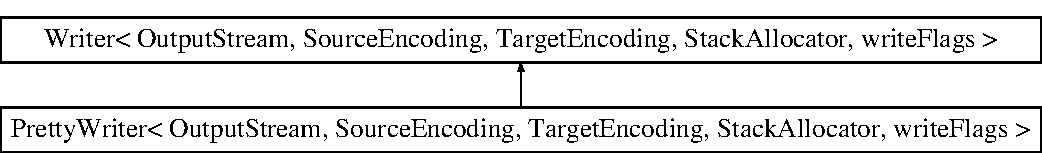
\includegraphics[height=2.000000cm]{classPrettyWriter}
\end{center}
\end{figure}
\subsection*{Public Types}
\begin{DoxyCompactItemize}
\item 
typedef \hyperlink{classWriter}{Writer}$<$ Output\+Stream, Source\+Encoding, Target\+Encoding, Stack\+Allocator, write\+Flags $>$ {\bfseries Base}\hypertarget{classPrettyWriter_a6eecc5c896dcdaffca739dcd39d13a17}{}\label{classPrettyWriter_a6eecc5c896dcdaffca739dcd39d13a17}

\item 
typedef Base\+::\+Ch {\bfseries Ch}\hypertarget{classPrettyWriter_ae35c89bda4c5d59d3ff6efcf2fea45a3}{}\label{classPrettyWriter_ae35c89bda4c5d59d3ff6efcf2fea45a3}

\end{DoxyCompactItemize}
\subsection*{Public Member Functions}
\begin{DoxyCompactItemize}
\item 
\hyperlink{classPrettyWriter_a928ac2a5235b8877048ebdd5f35a556f}{Pretty\+Writer} (Output\+Stream \&os, Stack\+Allocator $\ast$allocator=0, size\+\_\+t level\+Depth=Base\+::k\+Default\+Level\+Depth)
\begin{DoxyCompactList}\small\item\em Constructor. \end{DoxyCompactList}\item 
{\bfseries Pretty\+Writer} (Stack\+Allocator $\ast$allocator=0, size\+\_\+t level\+Depth=Base\+::k\+Default\+Level\+Depth)\hypertarget{classPrettyWriter_a4a9077e0300c6b0e1c830a58c1e738d2}{}\label{classPrettyWriter_a4a9077e0300c6b0e1c830a58c1e738d2}

\item 
\hyperlink{classPrettyWriter}{Pretty\+Writer} \& \hyperlink{classPrettyWriter_ad307b4c8d61af25042d0adcd0910c19a}{Set\+Indent} (Ch indent\+Char, unsigned indent\+Char\+Count)
\begin{DoxyCompactList}\small\item\em Set custom indentation. \end{DoxyCompactList}\item 
\hyperlink{classPrettyWriter}{Pretty\+Writer} \& \hyperlink{classPrettyWriter_a1ff9dbeff9b9c724080cb65987a41b73}{Set\+Format\+Options} (Pretty\+Format\+Options options)
\begin{DoxyCompactList}\small\item\em Set pretty writer formatting options. \end{DoxyCompactList}\item 
bool \hyperlink{classPrettyWriter_a440890a72408a150ef46edda6becdc94}{Raw\+Value} (const Ch $\ast$json, size\+\_\+t length, \hyperlink{rapidjson_8h_a1d1cfd8ffb84e947f82999c682b666a7}{Type} type)
\begin{DoxyCompactList}\small\item\em Write a raw J\+S\+ON value. \end{DoxyCompactList}\end{DoxyCompactItemize}
\begin{Indent}{\bf Implementation of Handler}\par
{\em \begin{DoxySeeAlso}{See also}
Handler 
\end{DoxySeeAlso}
}\begin{DoxyCompactItemize}
\item 
bool {\bfseries Null} ()\hypertarget{classPrettyWriter_aa144f2d0f0c3c69248cdbe957349528c}{}\label{classPrettyWriter_aa144f2d0f0c3c69248cdbe957349528c}

\item 
bool {\bfseries Bool} (bool b)\hypertarget{classPrettyWriter_a6e765ee7ada5ed40f317c78a98f6f90b}{}\label{classPrettyWriter_a6e765ee7ada5ed40f317c78a98f6f90b}

\item 
bool {\bfseries Int} (int i)\hypertarget{classPrettyWriter_aa1815263e61cb7af3b6dfba480a0f481}{}\label{classPrettyWriter_aa1815263e61cb7af3b6dfba480a0f481}

\item 
bool {\bfseries Uint} (unsigned u)\hypertarget{classPrettyWriter_a8c82302877a5588eae77eb7d042c49ef}{}\label{classPrettyWriter_a8c82302877a5588eae77eb7d042c49ef}

\item 
bool {\bfseries Int64} (int64\+\_\+t i64)\hypertarget{classPrettyWriter_ad42b797429f4ee19efdce610f5aff976}{}\label{classPrettyWriter_ad42b797429f4ee19efdce610f5aff976}

\item 
bool {\bfseries Uint64} (uint64\+\_\+t u64)\hypertarget{classPrettyWriter_aba75ac1f13c2629b2a55ffbf3d8a116c}{}\label{classPrettyWriter_aba75ac1f13c2629b2a55ffbf3d8a116c}

\item 
bool {\bfseries Double} (double d)\hypertarget{classPrettyWriter_ad9d592e86b985da666665926e87db415}{}\label{classPrettyWriter_ad9d592e86b985da666665926e87db415}

\item 
bool {\bfseries Raw\+Number} (const Ch $\ast$str, \hyperlink{rapidjson_8h_a5ed6e6e67250fadbd041127e6386dcb5}{Size\+Type} length, bool copy=false)\hypertarget{classPrettyWriter_a3941bc21d6a261ca8a86eff330db30ef}{}\label{classPrettyWriter_a3941bc21d6a261ca8a86eff330db30ef}

\item 
bool {\bfseries String} (const Ch $\ast$str, \hyperlink{rapidjson_8h_a5ed6e6e67250fadbd041127e6386dcb5}{Size\+Type} length, bool copy=false)\hypertarget{classPrettyWriter_ae544ccfe35dd7e80ed694873062409f6}{}\label{classPrettyWriter_ae544ccfe35dd7e80ed694873062409f6}

\item 
bool {\bfseries Start\+Object} ()\hypertarget{classPrettyWriter_a27bdda225dc152b8974e44c1df7525b7}{}\label{classPrettyWriter_a27bdda225dc152b8974e44c1df7525b7}

\item 
bool {\bfseries Key} (const Ch $\ast$str, \hyperlink{rapidjson_8h_a5ed6e6e67250fadbd041127e6386dcb5}{Size\+Type} length, bool copy=false)\hypertarget{classPrettyWriter_a20ecbe1d31a871e4da4a3899b40ad3cd}{}\label{classPrettyWriter_a20ecbe1d31a871e4da4a3899b40ad3cd}

\item 
bool {\bfseries End\+Object} (\hyperlink{rapidjson_8h_a5ed6e6e67250fadbd041127e6386dcb5}{Size\+Type} member\+Count=0)\hypertarget{classPrettyWriter_a6bfdfa4193193ef763cce5c592c4d20c}{}\label{classPrettyWriter_a6bfdfa4193193ef763cce5c592c4d20c}

\item 
bool {\bfseries Start\+Array} ()\hypertarget{classPrettyWriter_aec7fdf4798a3af5e31c147633f4798ed}{}\label{classPrettyWriter_aec7fdf4798a3af5e31c147633f4798ed}

\item 
bool {\bfseries End\+Array} (\hyperlink{rapidjson_8h_a5ed6e6e67250fadbd041127e6386dcb5}{Size\+Type} member\+Count=0)\hypertarget{classPrettyWriter_a1e9d97fc950d349f55abd864c787ff37}{}\label{classPrettyWriter_a1e9d97fc950d349f55abd864c787ff37}

\end{DoxyCompactItemize}
\end{Indent}
\begin{Indent}{\bf Convenience extensions}\par
\begin{DoxyCompactItemize}
\item 
bool \hyperlink{classPrettyWriter_a7e85689355a827d273f272c26b447225}{String} (const Ch $\ast$str)\hypertarget{classPrettyWriter_a7e85689355a827d273f272c26b447225}{}\label{classPrettyWriter_a7e85689355a827d273f272c26b447225}

\begin{DoxyCompactList}\small\item\em Simpler but slower overload. \end{DoxyCompactList}\item 
bool {\bfseries Key} (const Ch $\ast$str)\hypertarget{classPrettyWriter_a4b2a2a6eef02c12d7a3fd77966bd4499}{}\label{classPrettyWriter_a4b2a2a6eef02c12d7a3fd77966bd4499}

\end{DoxyCompactItemize}
\end{Indent}
\subsection*{Protected Member Functions}
\begin{DoxyCompactItemize}
\item 
void {\bfseries Pretty\+Prefix} (\hyperlink{rapidjson_8h_a1d1cfd8ffb84e947f82999c682b666a7}{Type} type)\hypertarget{classPrettyWriter_a09709ffa3b545e007631ecfd35029843}{}\label{classPrettyWriter_a09709ffa3b545e007631ecfd35029843}

\item 
void {\bfseries Write\+Indent} ()\hypertarget{classPrettyWriter_a6f244ecc94fd5b134d424033b1574b7e}{}\label{classPrettyWriter_a6f244ecc94fd5b134d424033b1574b7e}

\end{DoxyCompactItemize}
\subsection*{Protected Attributes}
\begin{DoxyCompactItemize}
\item 
Ch {\bfseries indent\+Char\+\_\+}\hypertarget{classPrettyWriter_aaa3f6380daa8466a5101ed18fc33bf04}{}\label{classPrettyWriter_aaa3f6380daa8466a5101ed18fc33bf04}

\item 
unsigned {\bfseries indent\+Char\+Count\+\_\+}\hypertarget{classPrettyWriter_a7d00b9716ef3cd7e34ae1b744c968f13}{}\label{classPrettyWriter_a7d00b9716ef3cd7e34ae1b744c968f13}

\item 
Pretty\+Format\+Options {\bfseries format\+Options\+\_\+}\hypertarget{classPrettyWriter_a15505ed4ea0fa85d339b3a987f1a3aaf}{}\label{classPrettyWriter_a15505ed4ea0fa85d339b3a987f1a3aaf}

\end{DoxyCompactItemize}
\subsection*{Additional Inherited Members}


\subsection{Detailed Description}
\subsubsection*{template$<$typename Output\+Stream, typename Source\+Encoding = U\+T\+F8$<$$>$, typename Target\+Encoding = U\+T\+F8$<$$>$, typename Stack\+Allocator = Crt\+Allocator, unsigned write\+Flags = k\+Write\+Default\+Flags$>$\\*
class Pretty\+Writer$<$ Output\+Stream, Source\+Encoding, Target\+Encoding, Stack\+Allocator, write\+Flags $>$}

\hyperlink{classWriter}{Writer} with indentation and spacing. 


\begin{DoxyTemplParams}{Template Parameters}
{\em Output\+Stream} & Type of ouptut os. \\
\hline
{\em Source\+Encoding} & Encoding of source string. \\
\hline
{\em Target\+Encoding} & Encoding of output stream. \\
\hline
{\em Stack\+Allocator} & Type of allocator for allocating memory of stack. \\
\hline
\end{DoxyTemplParams}


\subsection{Constructor \& Destructor Documentation}
\index{Pretty\+Writer@{Pretty\+Writer}!Pretty\+Writer@{Pretty\+Writer}}
\index{Pretty\+Writer@{Pretty\+Writer}!Pretty\+Writer@{Pretty\+Writer}}
\subsubsection[{\texorpdfstring{Pretty\+Writer(\+Output\+Stream \&os, Stack\+Allocator $\ast$allocator=0, size\+\_\+t level\+Depth=\+Base\+::k\+Default\+Level\+Depth)}{PrettyWriter(OutputStream &os, StackAllocator *allocator=0, size_t levelDepth=Base::kDefaultLevelDepth)}}]{\setlength{\rightskip}{0pt plus 5cm}template$<$typename Output\+Stream , typename Source\+Encoding  = U\+T\+F8$<$$>$, typename Target\+Encoding  = U\+T\+F8$<$$>$, typename Stack\+Allocator  = Crt\+Allocator, unsigned write\+Flags = k\+Write\+Default\+Flags$>$ {\bf Pretty\+Writer}$<$ Output\+Stream, Source\+Encoding, Target\+Encoding, Stack\+Allocator, write\+Flags $>$\+::{\bf Pretty\+Writer} (
\begin{DoxyParamCaption}
\item[{Output\+Stream \&}]{os, }
\item[{Stack\+Allocator $\ast$}]{allocator = {\ttfamily 0}, }
\item[{size\+\_\+t}]{level\+Depth = {\ttfamily Base\+:\+:kDefaultLevelDepth}}
\end{DoxyParamCaption}
)\hspace{0.3cm}{\ttfamily [inline]}, {\ttfamily [explicit]}}\hypertarget{classPrettyWriter_a928ac2a5235b8877048ebdd5f35a556f}{}\label{classPrettyWriter_a928ac2a5235b8877048ebdd5f35a556f}


Constructor. 


\begin{DoxyParams}{Parameters}
{\em os} & Output stream. \\
\hline
{\em allocator} & User supplied allocator. If it is null, it will create a private one. \\
\hline
{\em level\+Depth} & Initial capacity of stack. \\
\hline
\end{DoxyParams}


\subsection{Member Function Documentation}
\index{Pretty\+Writer@{Pretty\+Writer}!Raw\+Value@{Raw\+Value}}
\index{Raw\+Value@{Raw\+Value}!Pretty\+Writer@{Pretty\+Writer}}
\subsubsection[{\texorpdfstring{Raw\+Value(const Ch $\ast$json, size\+\_\+t length, Type type)}{RawValue(const Ch *json, size_t length, Type type)}}]{\setlength{\rightskip}{0pt plus 5cm}template$<$typename Output\+Stream , typename Source\+Encoding  = U\+T\+F8$<$$>$, typename Target\+Encoding  = U\+T\+F8$<$$>$, typename Stack\+Allocator  = Crt\+Allocator, unsigned write\+Flags = k\+Write\+Default\+Flags$>$ bool {\bf Pretty\+Writer}$<$ Output\+Stream, Source\+Encoding, Target\+Encoding, Stack\+Allocator, write\+Flags $>$\+::Raw\+Value (
\begin{DoxyParamCaption}
\item[{const Ch $\ast$}]{json, }
\item[{size\+\_\+t}]{length, }
\item[{{\bf Type}}]{type}
\end{DoxyParamCaption}
)\hspace{0.3cm}{\ttfamily [inline]}}\hypertarget{classPrettyWriter_a440890a72408a150ef46edda6becdc94}{}\label{classPrettyWriter_a440890a72408a150ef46edda6becdc94}


Write a raw J\+S\+ON value. 

For user to write a stringified J\+S\+ON as a value.


\begin{DoxyParams}{Parameters}
{\em json} & A well-\/formed J\+S\+ON value. It should not contain null character within \mbox{[}0, length -\/ 1\mbox{]} range. \\
\hline
{\em length} & Length of the json. \\
\hline
{\em type} & Type of the root of json. \\
\hline
\end{DoxyParams}
\begin{DoxyNote}{Note}
When using \hyperlink{classPrettyWriter_a440890a72408a150ef46edda6becdc94}{Pretty\+Writer\+::\+Raw\+Value()}, the result json may not be indented correctly. 
\end{DoxyNote}
\index{Pretty\+Writer@{Pretty\+Writer}!Set\+Format\+Options@{Set\+Format\+Options}}
\index{Set\+Format\+Options@{Set\+Format\+Options}!Pretty\+Writer@{Pretty\+Writer}}
\subsubsection[{\texorpdfstring{Set\+Format\+Options(\+Pretty\+Format\+Options options)}{SetFormatOptions(PrettyFormatOptions options)}}]{\setlength{\rightskip}{0pt plus 5cm}template$<$typename Output\+Stream , typename Source\+Encoding  = U\+T\+F8$<$$>$, typename Target\+Encoding  = U\+T\+F8$<$$>$, typename Stack\+Allocator  = Crt\+Allocator, unsigned write\+Flags = k\+Write\+Default\+Flags$>$ {\bf Pretty\+Writer}\& {\bf Pretty\+Writer}$<$ Output\+Stream, Source\+Encoding, Target\+Encoding, Stack\+Allocator, write\+Flags $>$\+::Set\+Format\+Options (
\begin{DoxyParamCaption}
\item[{Pretty\+Format\+Options}]{options}
\end{DoxyParamCaption}
)\hspace{0.3cm}{\ttfamily [inline]}}\hypertarget{classPrettyWriter_a1ff9dbeff9b9c724080cb65987a41b73}{}\label{classPrettyWriter_a1ff9dbeff9b9c724080cb65987a41b73}


Set pretty writer formatting options. 


\begin{DoxyParams}{Parameters}
{\em options} & Formatting options. \\
\hline
\end{DoxyParams}
\index{Pretty\+Writer@{Pretty\+Writer}!Set\+Indent@{Set\+Indent}}
\index{Set\+Indent@{Set\+Indent}!Pretty\+Writer@{Pretty\+Writer}}
\subsubsection[{\texorpdfstring{Set\+Indent(\+Ch indent\+Char, unsigned indent\+Char\+Count)}{SetIndent(Ch indentChar, unsigned indentCharCount)}}]{\setlength{\rightskip}{0pt plus 5cm}template$<$typename Output\+Stream , typename Source\+Encoding  = U\+T\+F8$<$$>$, typename Target\+Encoding  = U\+T\+F8$<$$>$, typename Stack\+Allocator  = Crt\+Allocator, unsigned write\+Flags = k\+Write\+Default\+Flags$>$ {\bf Pretty\+Writer}\& {\bf Pretty\+Writer}$<$ Output\+Stream, Source\+Encoding, Target\+Encoding, Stack\+Allocator, write\+Flags $>$\+::Set\+Indent (
\begin{DoxyParamCaption}
\item[{Ch}]{indent\+Char, }
\item[{unsigned}]{indent\+Char\+Count}
\end{DoxyParamCaption}
)\hspace{0.3cm}{\ttfamily [inline]}}\hypertarget{classPrettyWriter_ad307b4c8d61af25042d0adcd0910c19a}{}\label{classPrettyWriter_ad307b4c8d61af25042d0adcd0910c19a}


Set custom indentation. 


\begin{DoxyParams}{Parameters}
{\em indent\+Char} & Character for indentation. Must be whitespace character (\textquotesingle{} \textquotesingle{}, \textquotesingle{}\textbackslash{}t\textquotesingle{}, \textquotesingle{}\textbackslash{}n\textquotesingle{}, \textquotesingle{}\textbackslash{}r\textquotesingle{}). \\
\hline
{\em indent\+Char\+Count} & Number of indent characters for each indentation level. \\
\hline
\end{DoxyParams}
\begin{DoxyNote}{Note}
The default indentation is 4 spaces. 
\end{DoxyNote}


The documentation for this class was generated from the following files\+:\begin{DoxyCompactItemize}
\item 
/home/mate/\+Documents/\+Programming/\+Research/\+Multilayer\+Network\+Model/\+Multilayer\+Network\+Model/src/external/rapidjson/fwd.\+h\item 
/home/mate/\+Documents/\+Programming/\+Research/\+Multilayer\+Network\+Model/\+Multilayer\+Network\+Model/src/external/rapidjson/prettywriter.\+h\end{DoxyCompactItemize}

\hypertarget{classEquationParser_1_1Scanner}{}\section{Equation\+Parser\+:\+:Scanner Class Reference}
\label{classEquationParser_1_1Scanner}\index{Equation\+Parser\+::\+Scanner@{Equation\+Parser\+::\+Scanner}}
Inheritance diagram for Equation\+Parser\+:\+:Scanner\+:\begin{figure}[H]
\begin{center}
\leavevmode
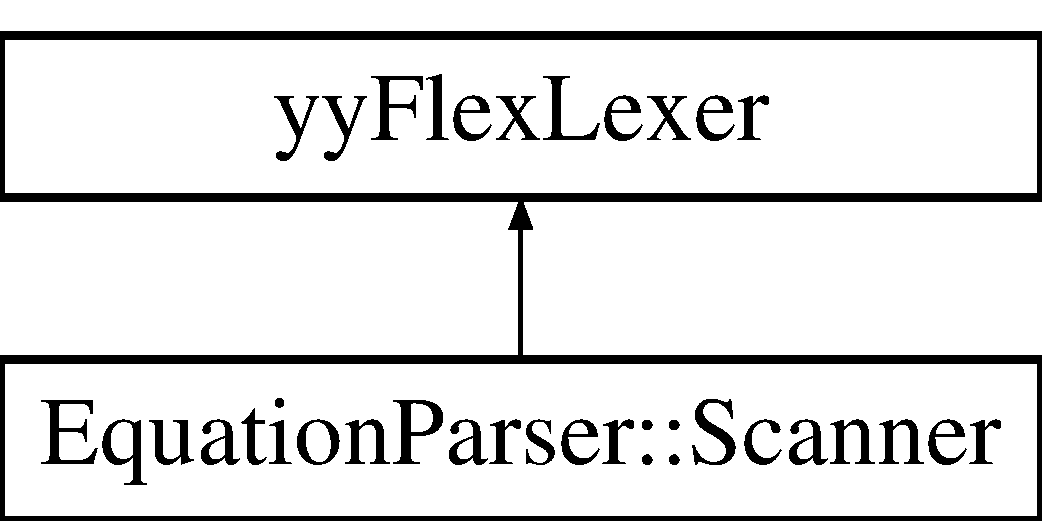
\includegraphics[height=2.000000cm]{classEquationParser_1_1Scanner}
\end{center}
\end{figure}
\subsection*{Public Member Functions}
\begin{DoxyCompactItemize}
\item 
{\bfseries Scanner} (\hyperlink{classEquationParser_1_1Interpreter}{Interpreter} \&driver)\hypertarget{classEquationParser_1_1Scanner_a383aac4a7ce836b3c656675aaeeb32a6}{}\label{classEquationParser_1_1Scanner_a383aac4a7ce836b3c656675aaeeb32a6}

\item 
virtual \hyperlink{classEquationParser_1_1Parser_ac7f402ded60cb9ac9bb65f5d2bc9d79c}{Equation\+Parser\+::\+Parser\+::symbol\+\_\+type} {\bfseries get\+\_\+next\+\_\+token} ()\hypertarget{classEquationParser_1_1Scanner_a679ce79f0470304c865aa1060dd7d5cd}{}\label{classEquationParser_1_1Scanner_a679ce79f0470304c865aa1060dd7d5cd}

\end{DoxyCompactItemize}


The documentation for this class was generated from the following file\+:\begin{DoxyCompactItemize}
\item 
/home/mate/\+Documents/\+Programming/\+Research/\+Multilayer\+Network\+Model/\+Multilayer\+Network\+Model/sources/parser/include/scanner.\+h\end{DoxyCompactItemize}

\hypertarget{classinternal_1_1Schema}{}\section{internal\+:\+:Schema$<$ Schema\+Document\+Type $>$ Class Template Reference}
\label{classinternal_1_1Schema}\index{internal\+::\+Schema$<$ Schema\+Document\+Type $>$@{internal\+::\+Schema$<$ Schema\+Document\+Type $>$}}
\subsection*{Public Types}
\begin{DoxyCompactItemize}
\item 
typedef Schema\+Document\+Type\+::\+Value\+Type {\bfseries Value\+Type}\hypertarget{classinternal_1_1Schema_a8976b6d7e2a885483d0b51d941019340}{}\label{classinternal_1_1Schema_a8976b6d7e2a885483d0b51d941019340}

\item 
typedef Schema\+Document\+Type\+::\+Allocator\+Type {\bfseries Allocator\+Type}\hypertarget{classinternal_1_1Schema_a7af392edd81e610754cd2e6b4f82761c}{}\label{classinternal_1_1Schema_a7af392edd81e610754cd2e6b4f82761c}

\item 
typedef Schema\+Document\+Type\+::\+Pointer\+Type {\bfseries Pointer\+Type}\hypertarget{classinternal_1_1Schema_a13d7dbba6e4a77b10862546777c5aae8}{}\label{classinternal_1_1Schema_a13d7dbba6e4a77b10862546777c5aae8}

\item 
typedef Value\+Type\+::\+Encoding\+Type {\bfseries Encoding\+Type}\hypertarget{classinternal_1_1Schema_a9ea269c3ca8099c2a14b6519fe34efb1}{}\label{classinternal_1_1Schema_a9ea269c3ca8099c2a14b6519fe34efb1}

\item 
typedef Encoding\+Type\+::\+Ch {\bfseries Ch}\hypertarget{classinternal_1_1Schema_a98043fca39adbf8b42e7472e3d80d6fa}{}\label{classinternal_1_1Schema_a98043fca39adbf8b42e7472e3d80d6fa}

\item 
typedef \hyperlink{structinternal_1_1SchemaValidationContext}{Schema\+Validation\+Context}$<$ Schema\+Document\+Type $>$ {\bfseries Context}\hypertarget{classinternal_1_1Schema_ac3f54abfefe300c5610c1205869cfd66}{}\label{classinternal_1_1Schema_ac3f54abfefe300c5610c1205869cfd66}

\item 
typedef \hyperlink{classinternal_1_1Schema}{Schema}$<$ Schema\+Document\+Type $>$ {\bfseries Schema\+Type}\hypertarget{classinternal_1_1Schema_ac2556ebf7a7db971e1c1c0f76eb5786e}{}\label{classinternal_1_1Schema_ac2556ebf7a7db971e1c1c0f76eb5786e}

\item 
typedef \hyperlink{classGenericValue}{Generic\+Value}$<$ Encoding\+Type, Allocator\+Type $>$ {\bfseries S\+Value}\hypertarget{classinternal_1_1Schema_ab3a07540a27d4cc2b0e260290c5c5771}{}\label{classinternal_1_1Schema_ab3a07540a27d4cc2b0e260290c5c5771}

\end{DoxyCompactItemize}
\subsection*{Public Member Functions}
\begin{DoxyCompactItemize}
\item 
{\bfseries Schema} (Schema\+Document\+Type $\ast$schema\+Document, const Pointer\+Type \&p, const Value\+Type \&value, const Value\+Type \&document, Allocator\+Type $\ast$allocator)\hypertarget{classinternal_1_1Schema_a31cbb5eaff43df83253f57d51585dc1d}{}\label{classinternal_1_1Schema_a31cbb5eaff43df83253f57d51585dc1d}

\item 
bool {\bfseries Begin\+Value} (\hyperlink{structinternal_1_1SchemaValidationContext}{Context} \&context) const \hypertarget{classinternal_1_1Schema_a60be92e1be5daec58dca25732617ad1b}{}\label{classinternal_1_1Schema_a60be92e1be5daec58dca25732617ad1b}

\item 
R\+A\+P\+I\+D\+J\+S\+O\+N\+\_\+\+F\+O\+R\+C\+E\+I\+N\+L\+I\+NE bool {\bfseries End\+Value} (\hyperlink{structinternal_1_1SchemaValidationContext}{Context} \&context) const \hypertarget{classinternal_1_1Schema_a5ea07987ee41ba93eeeb6ff8fc1ea197}{}\label{classinternal_1_1Schema_a5ea07987ee41ba93eeeb6ff8fc1ea197}

\item 
bool {\bfseries Null} (\hyperlink{structinternal_1_1SchemaValidationContext}{Context} \&context) const \hypertarget{classinternal_1_1Schema_acf2fd31da6d4ce46142dac016af1c047}{}\label{classinternal_1_1Schema_acf2fd31da6d4ce46142dac016af1c047}

\item 
bool {\bfseries Bool} (\hyperlink{structinternal_1_1SchemaValidationContext}{Context} \&context, bool) const \hypertarget{classinternal_1_1Schema_af9b64174e5248f276864ae63ec478ebd}{}\label{classinternal_1_1Schema_af9b64174e5248f276864ae63ec478ebd}

\item 
bool {\bfseries Int} (\hyperlink{structinternal_1_1SchemaValidationContext}{Context} \&context, int i) const \hypertarget{classinternal_1_1Schema_a39286fc0bfdfe3be57b1cd61fe162f19}{}\label{classinternal_1_1Schema_a39286fc0bfdfe3be57b1cd61fe162f19}

\item 
bool {\bfseries Uint} (\hyperlink{structinternal_1_1SchemaValidationContext}{Context} \&context, unsigned u) const \hypertarget{classinternal_1_1Schema_af355dc00a672448f42caee5a3b62a273}{}\label{classinternal_1_1Schema_af355dc00a672448f42caee5a3b62a273}

\item 
bool {\bfseries Int64} (\hyperlink{structinternal_1_1SchemaValidationContext}{Context} \&context, int64\+\_\+t i) const \hypertarget{classinternal_1_1Schema_a4aa9da1fd0cb4c19dcaaeebbc8abf1dc}{}\label{classinternal_1_1Schema_a4aa9da1fd0cb4c19dcaaeebbc8abf1dc}

\item 
bool {\bfseries Uint64} (\hyperlink{structinternal_1_1SchemaValidationContext}{Context} \&context, uint64\+\_\+t u) const \hypertarget{classinternal_1_1Schema_afb862d9aee4bbe2aa99e0f44ec90b9d8}{}\label{classinternal_1_1Schema_afb862d9aee4bbe2aa99e0f44ec90b9d8}

\item 
bool {\bfseries Double} (\hyperlink{structinternal_1_1SchemaValidationContext}{Context} \&context, double d) const \hypertarget{classinternal_1_1Schema_aaf4ff1cb84013ff1a82ecb59cac38bfe}{}\label{classinternal_1_1Schema_aaf4ff1cb84013ff1a82ecb59cac38bfe}

\item 
bool {\bfseries String} (\hyperlink{structinternal_1_1SchemaValidationContext}{Context} \&context, const Ch $\ast$str, \hyperlink{rapidjson_8h_a5ed6e6e67250fadbd041127e6386dcb5}{Size\+Type} length, bool) const \hypertarget{classinternal_1_1Schema_a2bc7b83a75b84c241e733be9d356a2c4}{}\label{classinternal_1_1Schema_a2bc7b83a75b84c241e733be9d356a2c4}

\item 
bool {\bfseries Start\+Object} (\hyperlink{structinternal_1_1SchemaValidationContext}{Context} \&context) const \hypertarget{classinternal_1_1Schema_a907b715d5f817d337a3e18759f3ac0e4}{}\label{classinternal_1_1Schema_a907b715d5f817d337a3e18759f3ac0e4}

\item 
bool {\bfseries Key} (\hyperlink{structinternal_1_1SchemaValidationContext}{Context} \&context, const Ch $\ast$str, \hyperlink{rapidjson_8h_a5ed6e6e67250fadbd041127e6386dcb5}{Size\+Type} len, bool) const \hypertarget{classinternal_1_1Schema_af0855cd2ee33929513dd8b148bfa9017}{}\label{classinternal_1_1Schema_af0855cd2ee33929513dd8b148bfa9017}

\item 
bool {\bfseries End\+Object} (\hyperlink{structinternal_1_1SchemaValidationContext}{Context} \&context, \hyperlink{rapidjson_8h_a5ed6e6e67250fadbd041127e6386dcb5}{Size\+Type} member\+Count) const \hypertarget{classinternal_1_1Schema_ac66720d141d8c811cb2c71da05509618}{}\label{classinternal_1_1Schema_ac66720d141d8c811cb2c71da05509618}

\item 
bool {\bfseries Start\+Array} (\hyperlink{structinternal_1_1SchemaValidationContext}{Context} \&context) const \hypertarget{classinternal_1_1Schema_a6340166b92577ce0ef9b7735f66937ec}{}\label{classinternal_1_1Schema_a6340166b92577ce0ef9b7735f66937ec}

\item 
bool {\bfseries End\+Array} (\hyperlink{structinternal_1_1SchemaValidationContext}{Context} \&context, \hyperlink{rapidjson_8h_a5ed6e6e67250fadbd041127e6386dcb5}{Size\+Type} element\+Count) const \hypertarget{classinternal_1_1Schema_a58101f966bd7e51086d456b3d84653eb}{}\label{classinternal_1_1Schema_a58101f966bd7e51086d456b3d84653eb}

\end{DoxyCompactItemize}
\subsection*{Friends}
\begin{DoxyCompactItemize}
\item 
class {\bfseries Generic\+Schema\+Document$<$ Value\+Type, Allocator\+Type $>$}\hypertarget{classinternal_1_1Schema_a04f1d1acd0a5a7fda069c115970d52b3}{}\label{classinternal_1_1Schema_a04f1d1acd0a5a7fda069c115970d52b3}

\end{DoxyCompactItemize}


The documentation for this class was generated from the following file\+:\begin{DoxyCompactItemize}
\item 
/home/mate/\+Documents/\+Programming/\+Research/\+Multilayer\+Network\+Model/\+Multilayer\+Network\+Model/src/external/rapidjson/schema.\+h\end{DoxyCompactItemize}

\hypertarget{classSchemaValidatingReader}{}\section{Schema\+Validating\+Reader$<$ parse\+Flags, Input\+Stream, Source\+Encoding, Schema\+Document\+Type, Stack\+Allocator $>$ Class Template Reference}
\label{classSchemaValidatingReader}\index{Schema\+Validating\+Reader$<$ parse\+Flags, Input\+Stream, Source\+Encoding, Schema\+Document\+Type, Stack\+Allocator $>$@{Schema\+Validating\+Reader$<$ parse\+Flags, Input\+Stream, Source\+Encoding, Schema\+Document\+Type, Stack\+Allocator $>$}}


A helper class for parsing with validation.  




{\ttfamily \#include $<$schema.\+h$>$}

\subsection*{Public Types}
\begin{DoxyCompactItemize}
\item 
typedef Schema\+Document\+Type\+::\+Pointer\+Type {\bfseries Pointer\+Type}\hypertarget{classSchemaValidatingReader_a30ecf1b20ca5a1b79e0d5f4ceb3bf198}{}\label{classSchemaValidatingReader_a30ecf1b20ca5a1b79e0d5f4ceb3bf198}

\item 
typedef Input\+Stream\+::\+Ch {\bfseries Ch}\hypertarget{classSchemaValidatingReader_a6eb6f887a49dbb400800ab4fc01f02c7}{}\label{classSchemaValidatingReader_a6eb6f887a49dbb400800ab4fc01f02c7}

\end{DoxyCompactItemize}
\subsection*{Public Member Functions}
\begin{DoxyCompactItemize}
\item 
\hyperlink{classSchemaValidatingReader_ae7945b71687ad3dd13b9c3d096892eac}{Schema\+Validating\+Reader} (Input\+Stream \&is, const Schema\+Document\+Type \&sd)
\begin{DoxyCompactList}\small\item\em Constructor. \end{DoxyCompactList}\item 
{\footnotesize template$<$typename Handler $>$ }\\bool {\bfseries operator()} (Handler \&handler)\hypertarget{classSchemaValidatingReader_a7135d8d53aacd850fbce2901cca4a4c3}{}\label{classSchemaValidatingReader_a7135d8d53aacd850fbce2901cca4a4c3}

\item 
const \hyperlink{structParseResult}{Parse\+Result} \& {\bfseries Get\+Parse\+Result} () const \hypertarget{classSchemaValidatingReader_aa5445bcfe27eaa55b28961a0ad6e86c1}{}\label{classSchemaValidatingReader_aa5445bcfe27eaa55b28961a0ad6e86c1}

\item 
bool {\bfseries Is\+Valid} () const \hypertarget{classSchemaValidatingReader_a01576a2c4ee21a6c73071e5f445dc0bd}{}\label{classSchemaValidatingReader_a01576a2c4ee21a6c73071e5f445dc0bd}

\item 
const Pointer\+Type \& {\bfseries Get\+Invalid\+Schema\+Pointer} () const \hypertarget{classSchemaValidatingReader_aaf450fe1f71af00a783d197e81ec6786}{}\label{classSchemaValidatingReader_aaf450fe1f71af00a783d197e81ec6786}

\item 
const Ch $\ast$ {\bfseries Get\+Invalid\+Schema\+Keyword} () const \hypertarget{classSchemaValidatingReader_ac040fa8a06b5950b40f907cc5fbec201}{}\label{classSchemaValidatingReader_ac040fa8a06b5950b40f907cc5fbec201}

\item 
const Pointer\+Type \& {\bfseries Get\+Invalid\+Document\+Pointer} () const \hypertarget{classSchemaValidatingReader_a8e5fb64a2b4c76572501c3b3e611e0fb}{}\label{classSchemaValidatingReader_a8e5fb64a2b4c76572501c3b3e611e0fb}

\end{DoxyCompactItemize}


\subsection{Detailed Description}
\subsubsection*{template$<$unsigned parse\+Flags, typename Input\+Stream, typename Source\+Encoding, typename Schema\+Document\+Type = Schema\+Document, typename Stack\+Allocator = Crt\+Allocator$>$\\*
class Schema\+Validating\+Reader$<$ parse\+Flags, Input\+Stream, Source\+Encoding, Schema\+Document\+Type, Stack\+Allocator $>$}

A helper class for parsing with validation. 

This helper class is a functor, designed as a parameter of \hyperlink{classGenericDocument_a36fbc7d0a9595d26e0d2c8859d207d1f}{Generic\+Document\+::\+Populate()}.


\begin{DoxyTemplParams}{Template Parameters}
{\em parse\+Flags} & Combination of \hyperlink{reader_8h_ab7be7dabe6ffcba60fad441505583450}{Parse\+Flag}. \\
\hline
{\em Input\+Stream} & Type of input stream, implementing Stream concept. \\
\hline
{\em Source\+Encoding} & Encoding of the input stream. \\
\hline
{\em Schema\+Document\+Type} & Type of schema document. \\
\hline
{\em Stack\+Allocator} & Allocator type for stack. \\
\hline
\end{DoxyTemplParams}


\subsection{Constructor \& Destructor Documentation}
\index{Schema\+Validating\+Reader@{Schema\+Validating\+Reader}!Schema\+Validating\+Reader@{Schema\+Validating\+Reader}}
\index{Schema\+Validating\+Reader@{Schema\+Validating\+Reader}!Schema\+Validating\+Reader@{Schema\+Validating\+Reader}}
\subsubsection[{\texorpdfstring{Schema\+Validating\+Reader(\+Input\+Stream \&is, const Schema\+Document\+Type \&sd)}{SchemaValidatingReader(InputStream &is, const SchemaDocumentType &sd)}}]{\setlength{\rightskip}{0pt plus 5cm}template$<$unsigned parse\+Flags, typename Input\+Stream , typename Source\+Encoding , typename Schema\+Document\+Type  = Schema\+Document, typename Stack\+Allocator  = Crt\+Allocator$>$ {\bf Schema\+Validating\+Reader}$<$ parse\+Flags, Input\+Stream, Source\+Encoding, Schema\+Document\+Type, Stack\+Allocator $>$\+::{\bf Schema\+Validating\+Reader} (
\begin{DoxyParamCaption}
\item[{Input\+Stream \&}]{is, }
\item[{const Schema\+Document\+Type \&}]{sd}
\end{DoxyParamCaption}
)\hspace{0.3cm}{\ttfamily [inline]}}\hypertarget{classSchemaValidatingReader_ae7945b71687ad3dd13b9c3d096892eac}{}\label{classSchemaValidatingReader_ae7945b71687ad3dd13b9c3d096892eac}


Constructor. 


\begin{DoxyParams}{Parameters}
{\em is} & Input stream. \\
\hline
{\em sd} & Schema document. \\
\hline
\end{DoxyParams}


The documentation for this class was generated from the following file\+:\begin{DoxyCompactItemize}
\item 
/home/mate/\+Documents/\+Programming/\+Research/\+Multilayer\+Network\+Model/\+Multilayer\+Network\+Model/sources/external/rapidjson/schema.\+h\end{DoxyCompactItemize}

\hypertarget{structinternal_1_1SchemaValidationContext}{}\section{internal\+:\+:Schema\+Validation\+Context$<$ Schema\+Document\+Type $>$ Struct Template Reference}
\label{structinternal_1_1SchemaValidationContext}\index{internal\+::\+Schema\+Validation\+Context$<$ Schema\+Document\+Type $>$@{internal\+::\+Schema\+Validation\+Context$<$ Schema\+Document\+Type $>$}}
\subsection*{Public Types}
\begin{DoxyCompactItemize}
\item 
enum {\bfseries Pattern\+Validator\+Type} \{ {\bfseries k\+Pattern\+Validator\+Only}, 
{\bfseries k\+Pattern\+Validator\+With\+Property}, 
{\bfseries k\+Pattern\+Validator\+With\+Additional\+Property}
 \}\hypertarget{structinternal_1_1SchemaValidationContext_a4fb1b8fe7ecb9d4608e6b0ac0716826c}{}\label{structinternal_1_1SchemaValidationContext_a4fb1b8fe7ecb9d4608e6b0ac0716826c}

\item 
typedef \hyperlink{classinternal_1_1Schema}{Schema}$<$ Schema\+Document\+Type $>$ {\bfseries Schema\+Type}\hypertarget{structinternal_1_1SchemaValidationContext_a79b155ab3711b97b6e33ced450614397}{}\label{structinternal_1_1SchemaValidationContext_a79b155ab3711b97b6e33ced450614397}

\item 
typedef \hyperlink{classinternal_1_1ISchemaStateFactory}{I\+Schema\+State\+Factory}$<$ \hyperlink{classinternal_1_1Schema}{Schema\+Type} $>$ {\bfseries Schema\+Validator\+Factory\+Type}\hypertarget{structinternal_1_1SchemaValidationContext_a33fa91fd8e880d1adb9b891fe441f110}{}\label{structinternal_1_1SchemaValidationContext_a33fa91fd8e880d1adb9b891fe441f110}

\item 
typedef Schema\+Type\+::\+Value\+Type {\bfseries Value\+Type}\hypertarget{structinternal_1_1SchemaValidationContext_acc134e808d3a4dbe8834eb1a3e98e816}{}\label{structinternal_1_1SchemaValidationContext_acc134e808d3a4dbe8834eb1a3e98e816}

\item 
typedef Value\+Type\+::\+Ch {\bfseries Ch}\hypertarget{structinternal_1_1SchemaValidationContext_abd905cd1513b117f1db68b58d6c41daf}{}\label{structinternal_1_1SchemaValidationContext_abd905cd1513b117f1db68b58d6c41daf}

\end{DoxyCompactItemize}
\subsection*{Public Member Functions}
\begin{DoxyCompactItemize}
\item 
{\bfseries Schema\+Validation\+Context} (\hyperlink{classinternal_1_1ISchemaStateFactory}{Schema\+Validator\+Factory\+Type} \&f, const \hyperlink{classinternal_1_1Schema}{Schema\+Type} $\ast$s)\hypertarget{structinternal_1_1SchemaValidationContext_a4adc8f66779626c9da4a56e7a87dcfac}{}\label{structinternal_1_1SchemaValidationContext_a4adc8f66779626c9da4a56e7a87dcfac}

\end{DoxyCompactItemize}
\subsection*{Public Attributes}
\begin{DoxyCompactItemize}
\item 
\hyperlink{classinternal_1_1ISchemaStateFactory}{Schema\+Validator\+Factory\+Type} \& {\bfseries factory}\hypertarget{structinternal_1_1SchemaValidationContext_ae2661ad92602b4f12fbffadb3dab502e}{}\label{structinternal_1_1SchemaValidationContext_ae2661ad92602b4f12fbffadb3dab502e}

\item 
const \hyperlink{classinternal_1_1Schema}{Schema\+Type} $\ast$ {\bfseries schema}\hypertarget{structinternal_1_1SchemaValidationContext_af44336e8a612b77a0091cc57f8de1734}{}\label{structinternal_1_1SchemaValidationContext_af44336e8a612b77a0091cc57f8de1734}

\item 
const \hyperlink{classinternal_1_1Schema}{Schema\+Type} $\ast$ {\bfseries value\+Schema}\hypertarget{structinternal_1_1SchemaValidationContext_a34865d65fb3cbb01bc497d0efade0458}{}\label{structinternal_1_1SchemaValidationContext_a34865d65fb3cbb01bc497d0efade0458}

\item 
const Ch $\ast$ {\bfseries invalid\+Keyword}\hypertarget{structinternal_1_1SchemaValidationContext_a9f6a91ee46c70e55f287b1e9b219df21}{}\label{structinternal_1_1SchemaValidationContext_a9f6a91ee46c70e55f287b1e9b219df21}

\item 
void $\ast$ {\bfseries hasher}\hypertarget{structinternal_1_1SchemaValidationContext_a4b419775e207cf72834f895dc30ac596}{}\label{structinternal_1_1SchemaValidationContext_a4b419775e207cf72834f895dc30ac596}

\item 
void $\ast$ {\bfseries array\+Element\+Hash\+Codes}\hypertarget{structinternal_1_1SchemaValidationContext_a5b6ec1a5fde2215de14a65fcbb06edde}{}\label{structinternal_1_1SchemaValidationContext_a5b6ec1a5fde2215de14a65fcbb06edde}

\item 
\hyperlink{classinternal_1_1ISchemaValidator}{I\+Schema\+Validator} $\ast$$\ast$ {\bfseries validators}\hypertarget{structinternal_1_1SchemaValidationContext_a1d215b80511f602ebece5c83b875cdd9}{}\label{structinternal_1_1SchemaValidationContext_a1d215b80511f602ebece5c83b875cdd9}

\item 
\hyperlink{rapidjson_8h_a5ed6e6e67250fadbd041127e6386dcb5}{Size\+Type} {\bfseries validator\+Count}\hypertarget{structinternal_1_1SchemaValidationContext_a10e5e97640846f3c23eaaba0506bb4f7}{}\label{structinternal_1_1SchemaValidationContext_a10e5e97640846f3c23eaaba0506bb4f7}

\item 
\hyperlink{classinternal_1_1ISchemaValidator}{I\+Schema\+Validator} $\ast$$\ast$ {\bfseries pattern\+Properties\+Validators}\hypertarget{structinternal_1_1SchemaValidationContext_a758565f674e8fb2066ff0f89ee67a174}{}\label{structinternal_1_1SchemaValidationContext_a758565f674e8fb2066ff0f89ee67a174}

\item 
\hyperlink{rapidjson_8h_a5ed6e6e67250fadbd041127e6386dcb5}{Size\+Type} {\bfseries pattern\+Properties\+Validator\+Count}\hypertarget{structinternal_1_1SchemaValidationContext_a2b8a521d60d39472a1550b535028a353}{}\label{structinternal_1_1SchemaValidationContext_a2b8a521d60d39472a1550b535028a353}

\item 
const \hyperlink{classinternal_1_1Schema}{Schema\+Type} $\ast$$\ast$ {\bfseries pattern\+Properties\+Schemas}\hypertarget{structinternal_1_1SchemaValidationContext_a12c48f172fbaae2e883f9eb2614d860e}{}\label{structinternal_1_1SchemaValidationContext_a12c48f172fbaae2e883f9eb2614d860e}

\item 
\hyperlink{rapidjson_8h_a5ed6e6e67250fadbd041127e6386dcb5}{Size\+Type} {\bfseries pattern\+Properties\+Schema\+Count}\hypertarget{structinternal_1_1SchemaValidationContext_a77d48b63f006479ab8c77f8192558441}{}\label{structinternal_1_1SchemaValidationContext_a77d48b63f006479ab8c77f8192558441}

\item 
Pattern\+Validator\+Type {\bfseries value\+Pattern\+Validator\+Type}\hypertarget{structinternal_1_1SchemaValidationContext_acc1ba6a63e678d0efff8a63d617c4d0d}{}\label{structinternal_1_1SchemaValidationContext_acc1ba6a63e678d0efff8a63d617c4d0d}

\item 
Pattern\+Validator\+Type {\bfseries object\+Pattern\+Validator\+Type}\hypertarget{structinternal_1_1SchemaValidationContext_add156192946b251ded2e11e24cfa9898}{}\label{structinternal_1_1SchemaValidationContext_add156192946b251ded2e11e24cfa9898}

\item 
\hyperlink{rapidjson_8h_a5ed6e6e67250fadbd041127e6386dcb5}{Size\+Type} {\bfseries array\+Element\+Index}\hypertarget{structinternal_1_1SchemaValidationContext_a213dd0b8a746b1548bb28b12a17c2c1e}{}\label{structinternal_1_1SchemaValidationContext_a213dd0b8a746b1548bb28b12a17c2c1e}

\item 
bool $\ast$ {\bfseries property\+Exist}\hypertarget{structinternal_1_1SchemaValidationContext_a3e58787498af48ecceb97c47fb592d47}{}\label{structinternal_1_1SchemaValidationContext_a3e58787498af48ecceb97c47fb592d47}

\item 
bool {\bfseries in\+Array}\hypertarget{structinternal_1_1SchemaValidationContext_af18fc4ef754e8a52732e152854f06341}{}\label{structinternal_1_1SchemaValidationContext_af18fc4ef754e8a52732e152854f06341}

\item 
bool {\bfseries value\+Uniqueness}\hypertarget{structinternal_1_1SchemaValidationContext_a23e93ca88653ed878e3ddf290fc6bd9f}{}\label{structinternal_1_1SchemaValidationContext_a23e93ca88653ed878e3ddf290fc6bd9f}

\item 
bool {\bfseries array\+Uniqueness}\hypertarget{structinternal_1_1SchemaValidationContext_a0864c5e8155fe0064f17e8dcb31d93c7}{}\label{structinternal_1_1SchemaValidationContext_a0864c5e8155fe0064f17e8dcb31d93c7}

\end{DoxyCompactItemize}


The documentation for this struct was generated from the following file\+:\begin{DoxyCompactItemize}
\item 
/home/mate/\+Documents/\+Programming/\+Research/\+Multilayer\+Network\+Model/\+Multilayer\+Network\+Model/src/external/rapidjson/schema.\+h\end{DoxyCompactItemize}

\hypertarget{structGenericValue_1_1ShortString}{}\section{Generic\+Value$<$ Encoding, Allocator $>$\+:\+:Short\+String Struct Reference}
\label{structGenericValue_1_1ShortString}\index{Generic\+Value$<$ Encoding, Allocator $>$\+::\+Short\+String@{Generic\+Value$<$ Encoding, Allocator $>$\+::\+Short\+String}}
\subsection*{Public Types}
\begin{DoxyCompactItemize}
\item 
enum \{ {\bfseries Max\+Chars} = sizeof(static\+\_\+cast$<$Flag$\ast$$>$(0)-\/$>$payload) / sizeof(Ch), 
{\bfseries Max\+Size} = Max\+Chars -\/ 1, 
{\bfseries Len\+Pos} = Max\+Size
 \}\hypertarget{structGenericValue_1_1ShortString_a9458c3a0d0eda7bac977cb41f1a19360}{}\label{structGenericValue_1_1ShortString_a9458c3a0d0eda7bac977cb41f1a19360}

\end{DoxyCompactItemize}
\subsection*{Public Member Functions}
\begin{DoxyCompactItemize}
\item 
void {\bfseries Set\+Length} (\hyperlink{rapidjson_8h_a5ed6e6e67250fadbd041127e6386dcb5}{Size\+Type} len)\hypertarget{structGenericValue_1_1ShortString_adbfe8461e0cb0ccb2cb3825489e743c2}{}\label{structGenericValue_1_1ShortString_adbfe8461e0cb0ccb2cb3825489e743c2}

\item 
\hyperlink{rapidjson_8h_a5ed6e6e67250fadbd041127e6386dcb5}{Size\+Type} {\bfseries Get\+Length} () const \hypertarget{structGenericValue_1_1ShortString_a65bea5171312b2243a1ec70ec6fa93cd}{}\label{structGenericValue_1_1ShortString_a65bea5171312b2243a1ec70ec6fa93cd}

\end{DoxyCompactItemize}
\subsection*{Static Public Member Functions}
\begin{DoxyCompactItemize}
\item 
static bool {\bfseries Usable} (\hyperlink{rapidjson_8h_a5ed6e6e67250fadbd041127e6386dcb5}{Size\+Type} len)\hypertarget{structGenericValue_1_1ShortString_a73e40f625c1abbd84f95ac7fff8365f7}{}\label{structGenericValue_1_1ShortString_a73e40f625c1abbd84f95ac7fff8365f7}

\end{DoxyCompactItemize}
\subsection*{Public Attributes}
\begin{DoxyCompactItemize}
\item 
\hyperlink{classGenericValue_ade0e0ce64ccd5d852da57a35e720bafb}{Ch} {\bfseries str} \mbox{[}Max\+Chars\mbox{]}\hypertarget{structGenericValue_1_1ShortString_a444e24523d4cc33830d18a2cfcfd333b}{}\label{structGenericValue_1_1ShortString_a444e24523d4cc33830d18a2cfcfd333b}

\end{DoxyCompactItemize}


The documentation for this struct was generated from the following file\+:\begin{DoxyCompactItemize}
\item 
/home/mate/\+Documents/\+Programming/\+Research/\+Multilayer\+Network\+Model/\+Multilayer\+Network\+Model/src/external/rapidjson/\hyperlink{document_8h}{document.\+h}\end{DoxyCompactItemize}

\hypertarget{classEquationParser_1_1slice}{}\section{Equation\+Parser\+:\+:slice$<$ T, S $>$ Class Template Reference}
\label{classEquationParser_1_1slice}\index{Equation\+Parser\+::slice$<$ T, S $>$@{Equation\+Parser\+::slice$<$ T, S $>$}}


Present a slice of the top of a stack.  




{\ttfamily \#include $<$stack.\+hh$>$}

\subsection*{Public Member Functions}
\begin{DoxyCompactItemize}
\item 
{\bfseries slice} (const S \&\hyperlink{classEquationParser_1_1stack}{stack}, unsigned int range)\hypertarget{classEquationParser_1_1slice_aa6e11d2a5286d4c024712d20c695d84e}{}\label{classEquationParser_1_1slice_aa6e11d2a5286d4c024712d20c695d84e}

\item 
const T \& {\bfseries operator\mbox{[}$\,$\mbox{]}} (unsigned int i) const \hypertarget{classEquationParser_1_1slice_a19f1344bb2a3e5a354233063389d09b2}{}\label{classEquationParser_1_1slice_a19f1344bb2a3e5a354233063389d09b2}

\end{DoxyCompactItemize}


\subsection{Detailed Description}
\subsubsection*{template$<$class T, class S = stack$<$\+T$>$$>$\\*
class Equation\+Parser\+::slice$<$ T, S $>$}

Present a slice of the top of a stack. 

The documentation for this class was generated from the following file\+:\begin{DoxyCompactItemize}
\item 
/home/mate/\+Documents/\+Programming/\+Research/\+Multilayer\+Network\+Model/\+Multilayer\+Network\+Model/sources/parser/include/\hyperlink{stack_8hh}{stack.\+hh}\end{DoxyCompactItemize}

\hypertarget{classEquationParser_1_1stack}{}\section{Equation\+Parser\+:\+:stack$<$ T, S $>$ Class Template Reference}
\label{classEquationParser_1_1stack}\index{Equation\+Parser\+::stack$<$ T, S $>$@{Equation\+Parser\+::stack$<$ T, S $>$}}
\subsection*{Public Types}
\begin{DoxyCompactItemize}
\item 
typedef S\+::reverse\+\_\+iterator {\bfseries iterator}\hypertarget{classEquationParser_1_1stack_a4787206121915f47e3424ffc40905c83}{}\label{classEquationParser_1_1stack_a4787206121915f47e3424ffc40905c83}

\item 
typedef S\+::const\+\_\+reverse\+\_\+iterator {\bfseries const\+\_\+iterator}\hypertarget{classEquationParser_1_1stack_a9345af7f2b8beffb48a2d402aaf1dd0e}{}\label{classEquationParser_1_1stack_a9345af7f2b8beffb48a2d402aaf1dd0e}

\end{DoxyCompactItemize}
\subsection*{Public Member Functions}
\begin{DoxyCompactItemize}
\item 
{\bfseries stack} (unsigned int n)\hypertarget{classEquationParser_1_1stack_a53002141fd9188b408a956c78b891a3e}{}\label{classEquationParser_1_1stack_a53002141fd9188b408a956c78b891a3e}

\item 
T \& {\bfseries operator\mbox{[}$\,$\mbox{]}} (unsigned int i)\hypertarget{classEquationParser_1_1stack_a1d68e52008e13d065377e9ff08f77ae9}{}\label{classEquationParser_1_1stack_a1d68e52008e13d065377e9ff08f77ae9}

\item 
const T \& {\bfseries operator\mbox{[}$\,$\mbox{]}} (unsigned int i) const \hypertarget{classEquationParser_1_1stack_a2f3e008e3b0e588b07de9e3e954930c2}{}\label{classEquationParser_1_1stack_a2f3e008e3b0e588b07de9e3e954930c2}

\item 
void \hyperlink{classEquationParser_1_1stack_afc5b5cd27279d5f799ee82c741466f96}{push} (T \&t)
\item 
void {\bfseries pop} (unsigned int n=1)\hypertarget{classEquationParser_1_1stack_a1af06a61b6153db22d1de607eaed4123}{}\label{classEquationParser_1_1stack_a1af06a61b6153db22d1de607eaed4123}

\item 
void {\bfseries clear} ()\hypertarget{classEquationParser_1_1stack_a0eccf84dc36173fcbda371eabfdcb460}{}\label{classEquationParser_1_1stack_a0eccf84dc36173fcbda371eabfdcb460}

\item 
S\+::size\+\_\+type {\bfseries size} () const \hypertarget{classEquationParser_1_1stack_a9097fcced4344a312463ba3c1f5ca9c8}{}\label{classEquationParser_1_1stack_a9097fcced4344a312463ba3c1f5ca9c8}

\item 
const\+\_\+iterator {\bfseries begin} () const \hypertarget{classEquationParser_1_1stack_a46ee174796ba7b658cd4a5ec5f387a0c}{}\label{classEquationParser_1_1stack_a46ee174796ba7b658cd4a5ec5f387a0c}

\item 
const\+\_\+iterator {\bfseries end} () const \hypertarget{classEquationParser_1_1stack_a1a74d0ecd28746f2fa6a7c8ed104e09b}{}\label{classEquationParser_1_1stack_a1a74d0ecd28746f2fa6a7c8ed104e09b}

\end{DoxyCompactItemize}


\subsection{Member Function Documentation}
\index{Equation\+Parser\+::stack@{Equation\+Parser\+::stack}!push@{push}}
\index{push@{push}!Equation\+Parser\+::stack@{Equation\+Parser\+::stack}}
\subsubsection[{\texorpdfstring{push(\+T \&t)}{push(T &t)}}]{\setlength{\rightskip}{0pt plus 5cm}template$<$class T, class S = std\+::vector$<$\+T$>$$>$ void {\bf Equation\+Parser\+::stack}$<$ T, S $>$\+::push (
\begin{DoxyParamCaption}
\item[{T \&}]{t}
\end{DoxyParamCaption}
)\hspace{0.3cm}{\ttfamily [inline]}}\hypertarget{classEquationParser_1_1stack_afc5b5cd27279d5f799ee82c741466f96}{}\label{classEquationParser_1_1stack_afc5b5cd27279d5f799ee82c741466f96}
Steal the contents of {\itshape t}.

Close to move-\/semantics. 

The documentation for this class was generated from the following file\+:\begin{DoxyCompactItemize}
\item 
/home/mate/\+Documents/\+Programming/\+Research/\+Multilayer\+Network\+Model/\+Multilayer\+Network\+Model/src/parser/include/\hyperlink{stack_8hh}{stack.\+hh}\end{DoxyCompactItemize}

\hypertarget{classinternal_1_1Stack}{}\section{internal\+:\+:Stack$<$ Allocator $>$ Class Template Reference}
\label{classinternal_1_1Stack}\index{internal\+::\+Stack$<$ Allocator $>$@{internal\+::\+Stack$<$ Allocator $>$}}


A type-\/unsafe stack for storing different types of data.  




{\ttfamily \#include $<$stack.\+h$>$}

\subsection*{Public Member Functions}
\begin{DoxyCompactItemize}
\item 
{\bfseries Stack} (Allocator $\ast$allocator, size\+\_\+t stack\+Capacity)\hypertarget{classinternal_1_1Stack_af09ab91f9e5143deccf7c9af837f451e}{}\label{classinternal_1_1Stack_af09ab91f9e5143deccf7c9af837f451e}

\item 
void {\bfseries Swap} (\hyperlink{classinternal_1_1Stack}{Stack} \&rhs) R\+A\+P\+I\+D\+J\+S\+O\+N\+\_\+\+N\+O\+E\+X\+C\+E\+PT\hypertarget{classinternal_1_1Stack_a5e601199a21d84b1ac612f558be0f2c3}{}\label{classinternal_1_1Stack_a5e601199a21d84b1ac612f558be0f2c3}

\item 
void {\bfseries Clear} ()\hypertarget{classinternal_1_1Stack_a02da31665a372738e81ded2f7b7d598e}{}\label{classinternal_1_1Stack_a02da31665a372738e81ded2f7b7d598e}

\item 
void {\bfseries Shrink\+To\+Fit} ()\hypertarget{classinternal_1_1Stack_a3852b8494d69c91f6a238a51572e591e}{}\label{classinternal_1_1Stack_a3852b8494d69c91f6a238a51572e591e}

\item 
{\footnotesize template$<$typename T $>$ }\\R\+A\+P\+I\+D\+J\+S\+O\+N\+\_\+\+F\+O\+R\+C\+E\+I\+N\+L\+I\+NE void {\bfseries Reserve} (size\+\_\+t count=1)\hypertarget{classinternal_1_1Stack_a7ae5de892834b7fc16099eb5e23dd97c}{}\label{classinternal_1_1Stack_a7ae5de892834b7fc16099eb5e23dd97c}

\item 
{\footnotesize template$<$typename T $>$ }\\R\+A\+P\+I\+D\+J\+S\+O\+N\+\_\+\+F\+O\+R\+C\+E\+I\+N\+L\+I\+NE T $\ast$ {\bfseries Push} (size\+\_\+t count=1)\hypertarget{classinternal_1_1Stack_a8038223ec0ed6ea92bb5f48e645a25ca}{}\label{classinternal_1_1Stack_a8038223ec0ed6ea92bb5f48e645a25ca}

\item 
{\footnotesize template$<$typename T $>$ }\\R\+A\+P\+I\+D\+J\+S\+O\+N\+\_\+\+F\+O\+R\+C\+E\+I\+N\+L\+I\+NE T $\ast$ {\bfseries Push\+Unsafe} (size\+\_\+t count=1)\hypertarget{classinternal_1_1Stack_a63b4eabd209d4fc9b43027f4e5660532}{}\label{classinternal_1_1Stack_a63b4eabd209d4fc9b43027f4e5660532}

\item 
{\footnotesize template$<$typename T $>$ }\\T $\ast$ {\bfseries Pop} (size\+\_\+t count)\hypertarget{classinternal_1_1Stack_a8545a8ccba595ac6e4ade9784474aa1c}{}\label{classinternal_1_1Stack_a8545a8ccba595ac6e4ade9784474aa1c}

\item 
{\footnotesize template$<$typename T $>$ }\\T $\ast$ {\bfseries Top} ()\hypertarget{classinternal_1_1Stack_ab3ed5b4afed3c73c516678516d5e195b}{}\label{classinternal_1_1Stack_ab3ed5b4afed3c73c516678516d5e195b}

\item 
{\footnotesize template$<$typename T $>$ }\\const T $\ast$ {\bfseries Top} () const \hypertarget{classinternal_1_1Stack_aa76b4cd53b9c3c65e544d14565eda7ae}{}\label{classinternal_1_1Stack_aa76b4cd53b9c3c65e544d14565eda7ae}

\item 
{\footnotesize template$<$typename T $>$ }\\T $\ast$ {\bfseries End} ()\hypertarget{classinternal_1_1Stack_a54987ae8ad774dd3ee80a43d268ef080}{}\label{classinternal_1_1Stack_a54987ae8ad774dd3ee80a43d268ef080}

\item 
{\footnotesize template$<$typename T $>$ }\\const T $\ast$ {\bfseries End} () const \hypertarget{classinternal_1_1Stack_a439ba97dc85710d469c65c1815dd4484}{}\label{classinternal_1_1Stack_a439ba97dc85710d469c65c1815dd4484}

\item 
{\footnotesize template$<$typename T $>$ }\\T $\ast$ {\bfseries Bottom} ()\hypertarget{classinternal_1_1Stack_a10aa1bc716b82cb0a40b3a3b9d5efe87}{}\label{classinternal_1_1Stack_a10aa1bc716b82cb0a40b3a3b9d5efe87}

\item 
{\footnotesize template$<$typename T $>$ }\\const T $\ast$ {\bfseries Bottom} () const \hypertarget{classinternal_1_1Stack_ae5057459b0f4cbb0cb6b541f99f60e07}{}\label{classinternal_1_1Stack_ae5057459b0f4cbb0cb6b541f99f60e07}

\item 
bool {\bfseries Has\+Allocator} () const \hypertarget{classinternal_1_1Stack_a6cd7033d53a1da185ea6dc2e15f7234c}{}\label{classinternal_1_1Stack_a6cd7033d53a1da185ea6dc2e15f7234c}

\item 
Allocator \& {\bfseries Get\+Allocator} ()\hypertarget{classinternal_1_1Stack_ab01f693833dfe136f574d66547623cfa}{}\label{classinternal_1_1Stack_ab01f693833dfe136f574d66547623cfa}

\item 
bool {\bfseries Empty} () const \hypertarget{classinternal_1_1Stack_abf57d1c7b356d8acbbe0e79147ca4b5c}{}\label{classinternal_1_1Stack_abf57d1c7b356d8acbbe0e79147ca4b5c}

\item 
size\+\_\+t {\bfseries Get\+Size} () const \hypertarget{classinternal_1_1Stack_ade4a25fa82950619652a30aa3a807f58}{}\label{classinternal_1_1Stack_ade4a25fa82950619652a30aa3a807f58}

\item 
size\+\_\+t {\bfseries Get\+Capacity} () const \hypertarget{classinternal_1_1Stack_a61dea1ed780c07bb438d17c581ab0e48}{}\label{classinternal_1_1Stack_a61dea1ed780c07bb438d17c581ab0e48}

\end{DoxyCompactItemize}


\subsection{Detailed Description}
\subsubsection*{template$<$typename Allocator$>$\\*
class internal\+::\+Stack$<$ Allocator $>$}

A type-\/unsafe stack for storing different types of data. 


\begin{DoxyTemplParams}{Template Parameters}
{\em Allocator} & Allocator for allocating stack memory. \\
\hline
\end{DoxyTemplParams}


The documentation for this class was generated from the following file\+:\begin{DoxyCompactItemize}
\item 
/home/mate/\+Documents/\+Programming/\+Research/\+Multilayer\+Network\+Model/\+Multilayer\+Network\+Model/src/external/rapidjson/internal/stack.\+h\end{DoxyCompactItemize}

\hypertarget{classrapidjson_1_1Stream}{}\section{rapidjson\+:\+:Stream Class Reference}
\label{classrapidjson_1_1Stream}\index{rapidjson\+::\+Stream@{rapidjson\+::\+Stream}}


Concept for reading and writing characters.  




{\ttfamily \#include $<$stream.\+h$>$}



\subsection{Detailed Description}
Concept for reading and writing characters. 

For read-\/only stream, no need to implement Put\+Begin(), Put(), Flush() and Put\+End().

For write-\/only stream, only need to implement Put() and Flush().


\begin{DoxyCode}
concept Stream \{
    \textcolor{keyword}{typename} Ch;    

    Ch Peek() \textcolor{keyword}{const};

    Ch Take();

    \textcolor{keywordtype}{size\_t} Tell();

    Ch* PutBegin();

    \textcolor{keywordtype}{void} Put(Ch c);

    \textcolor{keywordtype}{void} Flush();

    \textcolor{keywordtype}{size\_t} PutEnd(Ch* begin);
\}
\end{DoxyCode}
 

The documentation for this class was generated from the following file\+:\begin{DoxyCompactItemize}
\item 
/home/mate/\+Documents/\+Programming/\+Research/\+Multilayer\+Network\+Model/\+Multilayer\+Network\+Model/src/external/rapidjson/stream.\+h\end{DoxyCompactItemize}

\hypertarget{classinternal_1_1StreamLocalCopy}{}\section{internal\+:\+:Stream\+Local\+Copy$<$ Stream, int $>$ Class Template Reference}
\label{classinternal_1_1StreamLocalCopy}\index{internal\+::\+Stream\+Local\+Copy$<$ Stream, int $>$@{internal\+::\+Stream\+Local\+Copy$<$ Stream, int $>$}}


The documentation for this class was generated from the following file\+:\begin{DoxyCompactItemize}
\item 
/home/mate/\+Documents/\+Programming/\+Research/\+Multilayer\+Network\+Model/\+Multilayer\+Network\+Model/sources/external/rapidjson/\hyperlink{reader_8h}{reader.\+h}\end{DoxyCompactItemize}

\hypertarget{classinternal_1_1StreamLocalCopy_3_01Stream_00_010_01_4}{}\section{internal\+:\+:Stream\+Local\+Copy$<$ Stream, 0 $>$ Class Template Reference}
\label{classinternal_1_1StreamLocalCopy_3_01Stream_00_010_01_4}\index{internal\+::\+Stream\+Local\+Copy$<$ Stream, 0 $>$@{internal\+::\+Stream\+Local\+Copy$<$ Stream, 0 $>$}}


Keep reference.  




{\ttfamily \#include $<$reader.\+h$>$}

\subsection*{Public Member Functions}
\begin{DoxyCompactItemize}
\item 
{\bfseries Stream\+Local\+Copy} (Stream \&original)\hypertarget{classinternal_1_1StreamLocalCopy_3_01Stream_00_010_01_4_ac684a7be07d79d6ddd274dc1150f4b79}{}\label{classinternal_1_1StreamLocalCopy_3_01Stream_00_010_01_4_ac684a7be07d79d6ddd274dc1150f4b79}

\end{DoxyCompactItemize}
\subsection*{Public Attributes}
\begin{DoxyCompactItemize}
\item 
Stream \& {\bfseries s}\hypertarget{classinternal_1_1StreamLocalCopy_3_01Stream_00_010_01_4_ad31147888384f4bd51eabc2d7acdc4b6}{}\label{classinternal_1_1StreamLocalCopy_3_01Stream_00_010_01_4_ad31147888384f4bd51eabc2d7acdc4b6}

\end{DoxyCompactItemize}


\subsection{Detailed Description}
\subsubsection*{template$<$typename Stream$>$\\*
class internal\+::\+Stream\+Local\+Copy$<$ Stream, 0 $>$}

Keep reference. 

The documentation for this class was generated from the following file\+:\begin{DoxyCompactItemize}
\item 
/home/mate/\+Documents/\+Programming/\+Research/\+Multilayer\+Network\+Model/\+Multilayer\+Network\+Model/sources/external/rapidjson/\hyperlink{reader_8h}{reader.\+h}\end{DoxyCompactItemize}

\hypertarget{classinternal_1_1StreamLocalCopy_3_01Stream_00_011_01_4}{}\section{internal\+:\+:Stream\+Local\+Copy$<$ Stream, 1 $>$ Class Template Reference}
\label{classinternal_1_1StreamLocalCopy_3_01Stream_00_011_01_4}\index{internal\+::\+Stream\+Local\+Copy$<$ Stream, 1 $>$@{internal\+::\+Stream\+Local\+Copy$<$ Stream, 1 $>$}}


Do copy optimization.  




{\ttfamily \#include $<$reader.\+h$>$}

\subsection*{Public Member Functions}
\begin{DoxyCompactItemize}
\item 
{\bfseries Stream\+Local\+Copy} (Stream \&original)\hypertarget{classinternal_1_1StreamLocalCopy_3_01Stream_00_011_01_4_aba475fed3eecc9f77ff059fdb7fe2a32}{}\label{classinternal_1_1StreamLocalCopy_3_01Stream_00_011_01_4_aba475fed3eecc9f77ff059fdb7fe2a32}

\end{DoxyCompactItemize}
\subsection*{Public Attributes}
\begin{DoxyCompactItemize}
\item 
Stream {\bfseries s}\hypertarget{classinternal_1_1StreamLocalCopy_3_01Stream_00_011_01_4_a1d3e8ae8756325df25715d4ffb9c1b44}{}\label{classinternal_1_1StreamLocalCopy_3_01Stream_00_011_01_4_a1d3e8ae8756325df25715d4ffb9c1b44}

\end{DoxyCompactItemize}


\subsection{Detailed Description}
\subsubsection*{template$<$typename Stream$>$\\*
class internal\+::\+Stream\+Local\+Copy$<$ Stream, 1 $>$}

Do copy optimization. 

The documentation for this class was generated from the following file\+:\begin{DoxyCompactItemize}
\item 
/home/mate/\+Documents/\+Programming/\+Research/\+Multilayer\+Network\+Model/\+Multilayer\+Network\+Model/sources/external/rapidjson/\hyperlink{reader_8h}{reader.\+h}\end{DoxyCompactItemize}

\hypertarget{structStreamTraits}{}\section{Stream\+Traits$<$ Stream $>$ Struct Template Reference}
\label{structStreamTraits}\index{Stream\+Traits$<$ Stream $>$@{Stream\+Traits$<$ Stream $>$}}


Provides additional information for stream.  




{\ttfamily \#include $<$stream.\+h$>$}

\subsection*{Public Types}
\begin{DoxyCompactItemize}
\item 
enum \{ {\bfseries copy\+Optimization} = 0
 \}\begin{DoxyCompactList}\small\item\em Whether to make local copy of stream for optimization during parsing. \end{DoxyCompactList}
\end{DoxyCompactItemize}


\subsection{Detailed Description}
\subsubsection*{template$<$typename Stream$>$\\*
struct Stream\+Traits$<$ Stream $>$}

Provides additional information for stream. 

By using traits pattern, this type provides a default configuration for stream. For custom stream, this type can be specialized for other configuration. See T\+E\+S\+T(\+Reader, Custom\+String\+Stream) in readertest.\+cpp for example. 

\subsection{Member Enumeration Documentation}
\subsubsection[{\texorpdfstring{anonymous enum}{anonymous enum}}]{\setlength{\rightskip}{0pt plus 5cm}template$<$typename Stream $>$ anonymous enum}\hypertarget{structStreamTraits_a396e8fd5cbb7c0a9e4c1f509e4d490f5}{}\label{structStreamTraits_a396e8fd5cbb7c0a9e4c1f509e4d490f5}


Whether to make local copy of stream for optimization during parsing. 

By default, for safety, streams do not use local copy optimization. Stream that can be copied fast should specialize this, like Stream\+Traits$<$\+String\+Stream$>$. 

The documentation for this struct was generated from the following file\+:\begin{DoxyCompactItemize}
\item 
/home/mate/\+Documents/\+Programming/\+Research/\+Multilayer\+Network\+Model/\+Multilayer\+Network\+Model/src/external/rapidjson/stream.\+h\end{DoxyCompactItemize}

\hypertarget{structStreamTraits_3_01GenericInsituStringStream_3_01Encoding_01_4_01_4}{}\section{Stream\+Traits$<$ Generic\+Insitu\+String\+Stream$<$ Encoding $>$ $>$ Struct Template Reference}
\label{structStreamTraits_3_01GenericInsituStringStream_3_01Encoding_01_4_01_4}\index{Stream\+Traits$<$ Generic\+Insitu\+String\+Stream$<$ Encoding $>$ $>$@{Stream\+Traits$<$ Generic\+Insitu\+String\+Stream$<$ Encoding $>$ $>$}}
\subsection*{Public Types}
\begin{DoxyCompactItemize}
\item 
enum \{ {\bfseries copy\+Optimization} = 1
 \}\hypertarget{structStreamTraits_3_01GenericInsituStringStream_3_01Encoding_01_4_01_4_a67a610522828f475093e1e3c3b51a793}{}\label{structStreamTraits_3_01GenericInsituStringStream_3_01Encoding_01_4_01_4_a67a610522828f475093e1e3c3b51a793}

\end{DoxyCompactItemize}


The documentation for this struct was generated from the following file\+:\begin{DoxyCompactItemize}
\item 
/home/mate/\+Documents/\+Programming/\+Research/\+Multilayer\+Network\+Model/\+Multilayer\+Network\+Model/src/external/rapidjson/stream.\+h\end{DoxyCompactItemize}

\hypertarget{structStreamTraits_3_01GenericStringStream_3_01Encoding_01_4_01_4}{}\section{Stream\+Traits$<$ Generic\+String\+Stream$<$ Encoding $>$ $>$ Struct Template Reference}
\label{structStreamTraits_3_01GenericStringStream_3_01Encoding_01_4_01_4}\index{Stream\+Traits$<$ Generic\+String\+Stream$<$ Encoding $>$ $>$@{Stream\+Traits$<$ Generic\+String\+Stream$<$ Encoding $>$ $>$}}
\subsection*{Public Types}
\begin{DoxyCompactItemize}
\item 
enum \{ {\bfseries copy\+Optimization} = 1
 \}\hypertarget{structStreamTraits_3_01GenericStringStream_3_01Encoding_01_4_01_4_a36081c50934bef71843a4d351a98612e}{}\label{structStreamTraits_3_01GenericStringStream_3_01Encoding_01_4_01_4_a36081c50934bef71843a4d351a98612e}

\end{DoxyCompactItemize}


The documentation for this struct was generated from the following file\+:\begin{DoxyCompactItemize}
\item 
/home/mate/\+Documents/\+Programming/\+Research/\+Multilayer\+Network\+Model/\+Multilayer\+Network\+Model/src/external/rapidjson/stream.\+h\end{DoxyCompactItemize}

\hypertarget{structGenericValue_1_1String}{}\section{Generic\+Value$<$ Encoding, Allocator $>$\+:\+:String Struct Reference}
\label{structGenericValue_1_1String}\index{Generic\+Value$<$ Encoding, Allocator $>$\+::\+String@{Generic\+Value$<$ Encoding, Allocator $>$\+::\+String}}
\subsection*{Public Attributes}
\begin{DoxyCompactItemize}
\item 
\hyperlink{rapidjson_8h_a5ed6e6e67250fadbd041127e6386dcb5}{Size\+Type} {\bfseries length}\hypertarget{structGenericValue_1_1String_ad6ffab0e093aa8db6e415812ff6443bf}{}\label{structGenericValue_1_1String_ad6ffab0e093aa8db6e415812ff6443bf}

\item 
\hyperlink{rapidjson_8h_a5ed6e6e67250fadbd041127e6386dcb5}{Size\+Type} \hyperlink{structGenericValue_1_1String_a73631052aeb72fbabb6eaab0175f858e}{hashcode}\hypertarget{structGenericValue_1_1String_a73631052aeb72fbabb6eaab0175f858e}{}\label{structGenericValue_1_1String_a73631052aeb72fbabb6eaab0175f858e}

\begin{DoxyCompactList}\small\item\em reserved \end{DoxyCompactList}\item 
const \hyperlink{classGenericValue_ade0e0ce64ccd5d852da57a35e720bafb}{Ch} $\ast$ {\bfseries str}\hypertarget{structGenericValue_1_1String_a4eebc5acf3f93ab833efd82abf3ba84d}{}\label{structGenericValue_1_1String_a4eebc5acf3f93ab833efd82abf3ba84d}

\end{DoxyCompactItemize}


The documentation for this struct was generated from the following file\+:\begin{DoxyCompactItemize}
\item 
/home/mate/\+Documents/\+Programming/\+Research/\+Multilayer\+Network\+Model/\+Multilayer\+Network\+Model/sources/external/rapidjson/\hyperlink{document_8h}{document.\+h}\end{DoxyCompactItemize}

\hypertarget{classStructureGeneratorImpl}{}\section{Structure\+Generator\+Impl Class Reference}
\label{classStructureGeneratorImpl}\index{Structure\+Generator\+Impl@{Structure\+Generator\+Impl}}
Inheritance diagram for Structure\+Generator\+Impl\+:\begin{figure}[H]
\begin{center}
\leavevmode
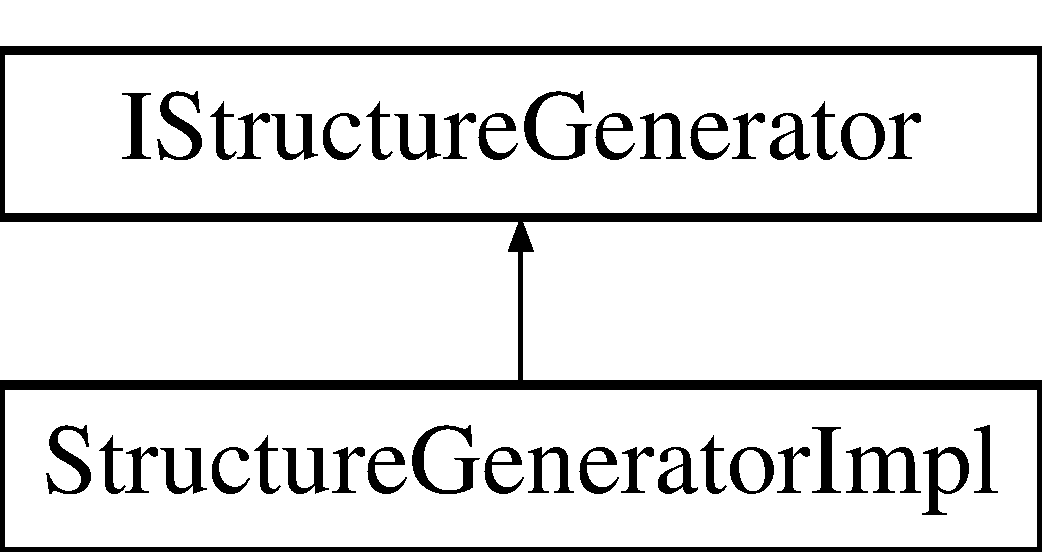
\includegraphics[height=2.000000cm]{classStructureGeneratorImpl}
\end{center}
\end{figure}
\subsection*{Public Member Functions}
\begin{DoxyCompactItemize}
\item 
{\bfseries Structure\+Generator\+Impl} (\hyperlink{classMultilayerNetwork}{Multilayer\+Network} $\ast$multilayer\+Network)\hypertarget{classStructureGeneratorImpl_a0e4efd8bc7d6f805054578026201ae38}{}\label{classStructureGeneratorImpl_a0e4efd8bc7d6f805054578026201ae38}

\item 
void {\bfseries generate\+Structure} ()\hypertarget{classStructureGeneratorImpl_a775184223dfef6f0e771589db2049993}{}\label{classStructureGeneratorImpl_a775184223dfef6f0e771589db2049993}

\end{DoxyCompactItemize}
\subsection*{Additional Inherited Members}


The documentation for this class was generated from the following files\+:\begin{DoxyCompactItemize}
\item 
/home/mate/\+Documents/\+Programming/\+Research/\+Multilayer\+Network\+Model/\+Multilayer\+Network\+Model/sources/generators/include/Structure\+Generator\+Impl.\+hh\item 
/home/mate/\+Documents/\+Programming/\+Research/\+Multilayer\+Network\+Model/\+Multilayer\+Network\+Model/sources/generators/src/Structure\+Generator\+Impl.\+cc\end{DoxyCompactItemize}

\hypertarget{structEquationParser_1_1Parser_1_1syntax__error}{}\section{Equation\+Parser\+:\+:Parser\+:\+:syntax\+\_\+error Struct Reference}
\label{structEquationParser_1_1Parser_1_1syntax__error}\index{Equation\+Parser\+::\+Parser\+::syntax\+\_\+error@{Equation\+Parser\+::\+Parser\+::syntax\+\_\+error}}


Syntax errors thrown from user actions.  




{\ttfamily \#include $<$parser.\+hpp$>$}

Inheritance diagram for Equation\+Parser\+:\+:Parser\+:\+:syntax\+\_\+error\+:\begin{figure}[H]
\begin{center}
\leavevmode
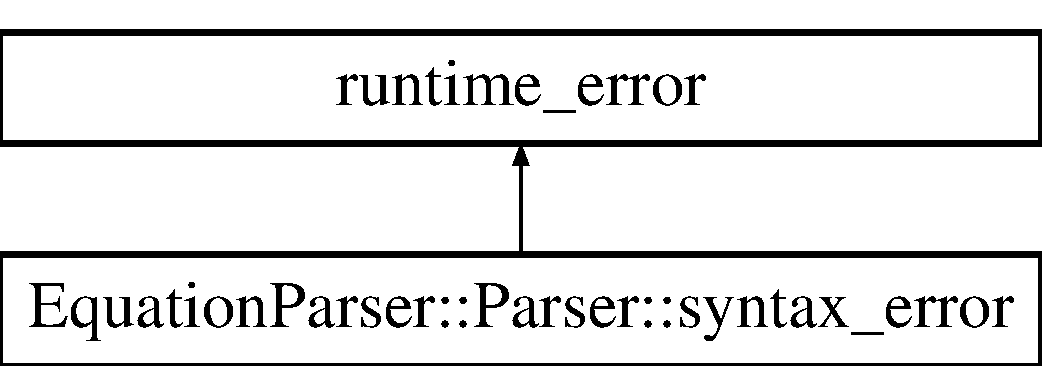
\includegraphics[height=2.000000cm]{structEquationParser_1_1Parser_1_1syntax__error}
\end{center}
\end{figure}
\subsection*{Public Member Functions}
\begin{DoxyCompactItemize}
\item 
{\bfseries syntax\+\_\+error} (const \hyperlink{classEquationParser_1_1Parser_a9c08ca33906dfb521b4ec5989e3620bf}{location\+\_\+type} \&l, const std\+::string \&m)\hypertarget{structEquationParser_1_1Parser_1_1syntax__error_a00d46855fc32f03ccd652f474d3b72ff}{}\label{structEquationParser_1_1Parser_1_1syntax__error_a00d46855fc32f03ccd652f474d3b72ff}

\end{DoxyCompactItemize}
\subsection*{Public Attributes}
\begin{DoxyCompactItemize}
\item 
\hyperlink{classEquationParser_1_1Parser_a9c08ca33906dfb521b4ec5989e3620bf}{location\+\_\+type} {\bfseries location}\hypertarget{structEquationParser_1_1Parser_1_1syntax__error_a2ed675b41cc29ee5864b24f6736ab809}{}\label{structEquationParser_1_1Parser_1_1syntax__error_a2ed675b41cc29ee5864b24f6736ab809}

\end{DoxyCompactItemize}


\subsection{Detailed Description}
Syntax errors thrown from user actions. 

The documentation for this struct was generated from the following file\+:\begin{DoxyCompactItemize}
\item 
/home/mate/\+Documents/\+Programming/\+Research/\+Multilayer\+Network\+Model/\+Multilayer\+Network\+Model/sources/parser/include/\hyperlink{parser_8hpp}{parser.\+hpp}\end{DoxyCompactItemize}

\hypertarget{structEquationParser_1_1Parser_1_1token}{}\section{Equation\+Parser\+:\+:Parser\+:\+:token Struct Reference}
\label{structEquationParser_1_1Parser_1_1token}\index{Equation\+Parser\+::\+Parser\+::token@{Equation\+Parser\+::\+Parser\+::token}}


Tokens.  




{\ttfamily \#include $<$parser.\+hpp$>$}

\subsection*{Public Types}
\begin{DoxyCompactItemize}
\item 
enum {\bfseries yytokentype} \{ \\*
{\bfseries T\+O\+K\+E\+N\+\_\+\+E\+ND} = 0, 
{\bfseries T\+O\+K\+E\+N\+\_\+\+S\+T\+R\+I\+NG} = 258, 
{\bfseries T\+O\+K\+E\+N\+\_\+\+L\+E\+F\+T\+P\+AR} = 259, 
{\bfseries T\+O\+K\+E\+N\+\_\+\+R\+I\+G\+H\+T\+P\+AR} = 260, 
\\*
{\bfseries T\+O\+K\+E\+N\+\_\+\+S\+E\+M\+I\+C\+O\+L\+ON} = 261, 
{\bfseries T\+O\+K\+E\+N\+\_\+\+C\+O\+M\+MA} = 262, 
{\bfseries T\+O\+K\+E\+N\+\_\+\+I\+N\+T\+E\+G\+ER} = 263, 
{\bfseries T\+O\+K\+E\+N\+\_\+\+D\+O\+U\+B\+LE} = 264, 
\\*
{\bfseries T\+O\+K\+E\+N\+\_\+\+P\+L\+US} = 265, 
{\bfseries T\+O\+K\+E\+N\+\_\+\+M\+I\+N\+US} = 266, 
{\bfseries T\+O\+K\+E\+N\+\_\+\+M\+U\+L\+T\+I\+P\+LY} = 267, 
{\bfseries T\+O\+K\+E\+N\+\_\+\+D\+I\+V\+I\+DE} = 268, 
\\*
{\bfseries T\+O\+K\+E\+N\+\_\+\+P\+O\+W\+ER} = 269
 \}\hypertarget{structEquationParser_1_1Parser_1_1token_a5696bebf3a1264ccfc2cf7c9a05a01c6}{}\label{structEquationParser_1_1Parser_1_1token_a5696bebf3a1264ccfc2cf7c9a05a01c6}

\end{DoxyCompactItemize}


\subsection{Detailed Description}
Tokens. 

The documentation for this struct was generated from the following file\+:\begin{DoxyCompactItemize}
\item 
/home/mate/\+Documents/\+Programming/\+Research/\+Multilayer\+Network\+Model/\+Multilayer\+Network\+Model/sources/parser/include/\hyperlink{parser_8hpp}{parser.\+hpp}\end{DoxyCompactItemize}

\hypertarget{structGenericPointer_1_1Token}{}\section{Generic\+Pointer$<$ Value\+Type, Allocator $>$\+:\+:Token Struct Reference}
\label{structGenericPointer_1_1Token}\index{Generic\+Pointer$<$ Value\+Type, Allocator $>$\+::\+Token@{Generic\+Pointer$<$ Value\+Type, Allocator $>$\+::\+Token}}


A token is the basic units of internal representation.  




{\ttfamily \#include $<$pointer.\+h$>$}

\subsection*{Public Attributes}
\begin{DoxyCompactItemize}
\item 
const \hyperlink{classGenericPointer_ab292356c11b4015c98d21b966b11f285}{Ch} $\ast$ \hyperlink{structGenericPointer_1_1Token_a8aa9b13bd66addb0c0512cfcae72174c}{name}\hypertarget{structGenericPointer_1_1Token_a8aa9b13bd66addb0c0512cfcae72174c}{}\label{structGenericPointer_1_1Token_a8aa9b13bd66addb0c0512cfcae72174c}

\begin{DoxyCompactList}\small\item\em Name of the token. It has null character at the end but it can contain null character. \end{DoxyCompactList}\item 
\hyperlink{rapidjson_8h_a5ed6e6e67250fadbd041127e6386dcb5}{Size\+Type} \hyperlink{structGenericPointer_1_1Token_a67383574032a3289d34002bb2d95df6d}{length}\hypertarget{structGenericPointer_1_1Token_a67383574032a3289d34002bb2d95df6d}{}\label{structGenericPointer_1_1Token_a67383574032a3289d34002bb2d95df6d}

\begin{DoxyCompactList}\small\item\em Length of the name. \end{DoxyCompactList}\item 
\hyperlink{rapidjson_8h_a5ed6e6e67250fadbd041127e6386dcb5}{Size\+Type} \hyperlink{structGenericPointer_1_1Token_a0ce571cfe3f3da942a5912bb2cd24dcf}{index}\hypertarget{structGenericPointer_1_1Token_a0ce571cfe3f3da942a5912bb2cd24dcf}{}\label{structGenericPointer_1_1Token_a0ce571cfe3f3da942a5912bb2cd24dcf}

\begin{DoxyCompactList}\small\item\em A valid array index, if it is not equal to k\+Pointer\+Invalid\+Index. \end{DoxyCompactList}\end{DoxyCompactItemize}


\subsection{Detailed Description}
\subsubsection*{template$<$typename Value\+Type, typename Allocator = Crt\+Allocator$>$\\*
struct Generic\+Pointer$<$ Value\+Type, Allocator $>$\+::\+Token}

A token is the basic units of internal representation. 

A J\+S\+ON pointer string representation \char`\"{}/foo/123\char`\"{} is parsed to two tokens\+: \char`\"{}foo\char`\"{} and 123. 123 will be represented in both numeric form and string form. They are resolved according to the actual value type (object or array).

For token that are not numbers, or the numeric value is out of bound (greater than limits of Size\+Type), they are only treated as string form (i.\+e. the token\textquotesingle{}s index will be equal to k\+Pointer\+Invalid\+Index).

This struct is public so that user can create a Pointer without parsing and allocation, using a special constructor. 

The documentation for this struct was generated from the following file\+:\begin{DoxyCompactItemize}
\item 
/home/mate/\+Documents/\+Programming/\+Research/\+Multilayer\+Network\+Model/\+Multilayer\+Network\+Model/src/external/rapidjson/pointer.\+h\end{DoxyCompactItemize}

\hypertarget{structinternal_1_1TokenHelper}{}\section{internal\+:\+:Token\+Helper$<$ Stack, Ch $>$ Struct Template Reference}
\label{structinternal_1_1TokenHelper}\index{internal\+::\+Token\+Helper$<$ Stack, Ch $>$@{internal\+::\+Token\+Helper$<$ Stack, Ch $>$}}
\subsection*{Static Public Member Functions}
\begin{DoxyCompactItemize}
\item 
static R\+A\+P\+I\+D\+J\+S\+O\+N\+\_\+\+F\+O\+R\+C\+E\+I\+N\+L\+I\+NE void {\bfseries Append\+Index\+Token} (\hyperlink{classinternal_1_1Stack}{Stack} \&document\+Stack, \hyperlink{rapidjson_8h_a5ed6e6e67250fadbd041127e6386dcb5}{Size\+Type} index)\hypertarget{structinternal_1_1TokenHelper_a7b1864bfe6d4014ba7a5114acb26b3ae}{}\label{structinternal_1_1TokenHelper_a7b1864bfe6d4014ba7a5114acb26b3ae}

\end{DoxyCompactItemize}


The documentation for this struct was generated from the following file\+:\begin{DoxyCompactItemize}
\item 
/home/mate/\+Documents/\+Programming/\+Research/\+Multilayer\+Network\+Model/\+Multilayer\+Network\+Model/sources/external/rapidjson/schema.\+h\end{DoxyCompactItemize}

\hypertarget{structinternal_1_1TokenHelper_3_01Stack_00_01char_01_4}{}\section{internal\+:\+:Token\+Helper$<$ Stack, char $>$ Struct Template Reference}
\label{structinternal_1_1TokenHelper_3_01Stack_00_01char_01_4}\index{internal\+::\+Token\+Helper$<$ Stack, char $>$@{internal\+::\+Token\+Helper$<$ Stack, char $>$}}
\subsection*{Static Public Member Functions}
\begin{DoxyCompactItemize}
\item 
static R\+A\+P\+I\+D\+J\+S\+O\+N\+\_\+\+F\+O\+R\+C\+E\+I\+N\+L\+I\+NE void {\bfseries Append\+Index\+Token} (\hyperlink{classinternal_1_1Stack}{Stack} \&document\+Stack, \hyperlink{rapidjson_8h_a5ed6e6e67250fadbd041127e6386dcb5}{Size\+Type} index)\hypertarget{structinternal_1_1TokenHelper_3_01Stack_00_01char_01_4_a5d635eb7590e098c3340c9e5dcc72ae3}{}\label{structinternal_1_1TokenHelper_3_01Stack_00_01char_01_4_a5d635eb7590e098c3340c9e5dcc72ae3}

\end{DoxyCompactItemize}


The documentation for this struct was generated from the following file\+:\begin{DoxyCompactItemize}
\item 
/home/mate/\+Documents/\+Programming/\+Research/\+Multilayer\+Network\+Model/\+Multilayer\+Network\+Model/sources/external/rapidjson/schema.\+h\end{DoxyCompactItemize}

\hypertarget{structTranscoder}{}\section{Transcoder$<$ Source\+Encoding, Target\+Encoding $>$ Struct Template Reference}
\label{structTranscoder}\index{Transcoder$<$ Source\+Encoding, Target\+Encoding $>$@{Transcoder$<$ Source\+Encoding, Target\+Encoding $>$}}


Encoding conversion.  




{\ttfamily \#include $<$encodings.\+h$>$}

\subsection*{Static Public Member Functions}
\begin{DoxyCompactItemize}
\item 
{\footnotesize template$<$typename Input\+Stream , typename Output\+Stream $>$ }\\static R\+A\+P\+I\+D\+J\+S\+O\+N\+\_\+\+F\+O\+R\+C\+E\+I\+N\+L\+I\+NE bool \hyperlink{structTranscoder_a0ea2edfe35784ebf1063921d2bd5fb66}{Transcode} (Input\+Stream \&is, Output\+Stream \&os)\hypertarget{structTranscoder_a0ea2edfe35784ebf1063921d2bd5fb66}{}\label{structTranscoder_a0ea2edfe35784ebf1063921d2bd5fb66}

\begin{DoxyCompactList}\small\item\em Take one Unicode codepoint from source encoding, convert it to target encoding and put it to the output stream. \end{DoxyCompactList}\item 
{\footnotesize template$<$typename Input\+Stream , typename Output\+Stream $>$ }\\static R\+A\+P\+I\+D\+J\+S\+O\+N\+\_\+\+F\+O\+R\+C\+E\+I\+N\+L\+I\+NE bool {\bfseries Transcode\+Unsafe} (Input\+Stream \&is, Output\+Stream \&os)\hypertarget{structTranscoder_a16345a912c679b2ea197328eb1444f82}{}\label{structTranscoder_a16345a912c679b2ea197328eb1444f82}

\item 
{\footnotesize template$<$typename Input\+Stream , typename Output\+Stream $>$ }\\static R\+A\+P\+I\+D\+J\+S\+O\+N\+\_\+\+F\+O\+R\+C\+E\+I\+N\+L\+I\+NE bool \hyperlink{structTranscoder_a8a64aa837f7962894a99f63232472543}{Validate} (Input\+Stream \&is, Output\+Stream \&os)\hypertarget{structTranscoder_a8a64aa837f7962894a99f63232472543}{}\label{structTranscoder_a8a64aa837f7962894a99f63232472543}

\begin{DoxyCompactList}\small\item\em Validate one Unicode codepoint from an encoded stream. \end{DoxyCompactList}\end{DoxyCompactItemize}


\subsection{Detailed Description}
\subsubsection*{template$<$typename Source\+Encoding, typename Target\+Encoding$>$\\*
struct Transcoder$<$ Source\+Encoding, Target\+Encoding $>$}

Encoding conversion. 

The documentation for this struct was generated from the following file\+:\begin{DoxyCompactItemize}
\item 
/home/mate/\+Documents/\+Programming/\+Research/\+Multilayer\+Network\+Model/\+Multilayer\+Network\+Model/src/external/rapidjson/encodings.\+h\end{DoxyCompactItemize}

\hypertarget{structTranscoder_3_01Encoding_00_01Encoding_01_4}{}\section{Transcoder$<$ Encoding, Encoding $>$ Struct Template Reference}
\label{structTranscoder_3_01Encoding_00_01Encoding_01_4}\index{Transcoder$<$ Encoding, Encoding $>$@{Transcoder$<$ Encoding, Encoding $>$}}


Specialization of \hyperlink{structTranscoder}{Transcoder} with same source and target encoding.  




{\ttfamily \#include $<$encodings.\+h$>$}

\subsection*{Static Public Member Functions}
\begin{DoxyCompactItemize}
\item 
{\footnotesize template$<$typename Input\+Stream , typename Output\+Stream $>$ }\\static R\+A\+P\+I\+D\+J\+S\+O\+N\+\_\+\+F\+O\+R\+C\+E\+I\+N\+L\+I\+NE bool {\bfseries Transcode} (Input\+Stream \&is, Output\+Stream \&os)\hypertarget{structTranscoder_3_01Encoding_00_01Encoding_01_4_aad11cdc2b829123a7b9969e34d456813}{}\label{structTranscoder_3_01Encoding_00_01Encoding_01_4_aad11cdc2b829123a7b9969e34d456813}

\item 
{\footnotesize template$<$typename Input\+Stream , typename Output\+Stream $>$ }\\static R\+A\+P\+I\+D\+J\+S\+O\+N\+\_\+\+F\+O\+R\+C\+E\+I\+N\+L\+I\+NE bool {\bfseries Transcode\+Unsafe} (Input\+Stream \&is, Output\+Stream \&os)\hypertarget{structTranscoder_3_01Encoding_00_01Encoding_01_4_addf67decfff7d0de510c47842eb53cef}{}\label{structTranscoder_3_01Encoding_00_01Encoding_01_4_addf67decfff7d0de510c47842eb53cef}

\item 
{\footnotesize template$<$typename Input\+Stream , typename Output\+Stream $>$ }\\static R\+A\+P\+I\+D\+J\+S\+O\+N\+\_\+\+F\+O\+R\+C\+E\+I\+N\+L\+I\+NE bool {\bfseries Validate} (Input\+Stream \&is, Output\+Stream \&os)\hypertarget{structTranscoder_3_01Encoding_00_01Encoding_01_4_a536aa3930251161d05e112947ec2f9c8}{}\label{structTranscoder_3_01Encoding_00_01Encoding_01_4_a536aa3930251161d05e112947ec2f9c8}

\end{DoxyCompactItemize}


\subsection{Detailed Description}
\subsubsection*{template$<$typename Encoding$>$\\*
struct Transcoder$<$ Encoding, Encoding $>$}

Specialization of \hyperlink{structTranscoder}{Transcoder} with same source and target encoding. 

The documentation for this struct was generated from the following file\+:\begin{DoxyCompactItemize}
\item 
/home/mate/\+Documents/\+Programming/\+Research/\+Multilayer\+Network\+Model/\+Multilayer\+Network\+Model/src/external/rapidjson/encodings.\+h\end{DoxyCompactItemize}

\hypertarget{structinternal_1_1TypeHelper}{}\section{internal\+:\+:Type\+Helper$<$ Value\+Type, T $>$ Struct Template Reference}
\label{structinternal_1_1TypeHelper}\index{internal\+::\+Type\+Helper$<$ Value\+Type, T $>$@{internal\+::\+Type\+Helper$<$ Value\+Type, T $>$}}


The documentation for this struct was generated from the following file\+:\begin{DoxyCompactItemize}
\item 
/home/mate/\+Documents/\+Programming/\+Research/\+Multilayer\+Network\+Model/\+Multilayer\+Network\+Model/sources/external/rapidjson/\hyperlink{document_8h}{document.\+h}\end{DoxyCompactItemize}

\hypertarget{structinternal_1_1TypeHelper_3_01ValueType_00_01bool_01_4}{}\section{internal\+:\+:Type\+Helper$<$ Value\+Type, bool $>$ Struct Template Reference}
\label{structinternal_1_1TypeHelper_3_01ValueType_00_01bool_01_4}\index{internal\+::\+Type\+Helper$<$ Value\+Type, bool $>$@{internal\+::\+Type\+Helper$<$ Value\+Type, bool $>$}}
\subsection*{Static Public Member Functions}
\begin{DoxyCompactItemize}
\item 
static bool {\bfseries Is} (const Value\+Type \&v)\hypertarget{structinternal_1_1TypeHelper_3_01ValueType_00_01bool_01_4_aa73fb8b4ed649706f7f9165401f89c27}{}\label{structinternal_1_1TypeHelper_3_01ValueType_00_01bool_01_4_aa73fb8b4ed649706f7f9165401f89c27}

\item 
static bool {\bfseries Get} (const Value\+Type \&v)\hypertarget{structinternal_1_1TypeHelper_3_01ValueType_00_01bool_01_4_aed612b233e5985d049248b414fb0034a}{}\label{structinternal_1_1TypeHelper_3_01ValueType_00_01bool_01_4_aed612b233e5985d049248b414fb0034a}

\item 
static Value\+Type \& {\bfseries Set} (Value\+Type \&v, bool data)\hypertarget{structinternal_1_1TypeHelper_3_01ValueType_00_01bool_01_4_a4bfa644e57e7d725468ed78103c1579a}{}\label{structinternal_1_1TypeHelper_3_01ValueType_00_01bool_01_4_a4bfa644e57e7d725468ed78103c1579a}

\item 
static Value\+Type \& {\bfseries Set} (Value\+Type \&v, bool data, typename Value\+Type\+::\+Allocator\+Type \&)\hypertarget{structinternal_1_1TypeHelper_3_01ValueType_00_01bool_01_4_a01a2bdf4117fb767c8d703be9e0f5f1d}{}\label{structinternal_1_1TypeHelper_3_01ValueType_00_01bool_01_4_a01a2bdf4117fb767c8d703be9e0f5f1d}

\end{DoxyCompactItemize}


The documentation for this struct was generated from the following file\+:\begin{DoxyCompactItemize}
\item 
/home/mate/\+Documents/\+Programming/\+Research/\+Multilayer\+Network\+Model/\+Multilayer\+Network\+Model/sources/external/rapidjson/\hyperlink{document_8h}{document.\+h}\end{DoxyCompactItemize}

\hypertarget{structinternal_1_1TypeHelper_3_01ValueType_00_01const_01typename_01ValueType_1_1Ch_01_5_01_4}{}\section{internal\+:\+:Type\+Helper$<$ Value\+Type, const typename Value\+Type\+:\+:Ch $\ast$ $>$ Struct Template Reference}
\label{structinternal_1_1TypeHelper_3_01ValueType_00_01const_01typename_01ValueType_1_1Ch_01_5_01_4}\index{internal\+::\+Type\+Helper$<$ Value\+Type, const typename Value\+Type\+::\+Ch $\ast$ $>$@{internal\+::\+Type\+Helper$<$ Value\+Type, const typename Value\+Type\+::\+Ch $\ast$ $>$}}
\subsection*{Public Types}
\begin{DoxyCompactItemize}
\item 
typedef const Value\+Type\+::\+Ch $\ast$ {\bfseries String\+Type}\hypertarget{structinternal_1_1TypeHelper_3_01ValueType_00_01const_01typename_01ValueType_1_1Ch_01_5_01_4_a61b7fd9c92eab60394fdff466251c399}{}\label{structinternal_1_1TypeHelper_3_01ValueType_00_01const_01typename_01ValueType_1_1Ch_01_5_01_4_a61b7fd9c92eab60394fdff466251c399}

\end{DoxyCompactItemize}
\subsection*{Static Public Member Functions}
\begin{DoxyCompactItemize}
\item 
static bool {\bfseries Is} (const Value\+Type \&v)\hypertarget{structinternal_1_1TypeHelper_3_01ValueType_00_01const_01typename_01ValueType_1_1Ch_01_5_01_4_a9543f180b6ac2b923486f1b69d5356ea}{}\label{structinternal_1_1TypeHelper_3_01ValueType_00_01const_01typename_01ValueType_1_1Ch_01_5_01_4_a9543f180b6ac2b923486f1b69d5356ea}

\item 
static String\+Type {\bfseries Get} (const Value\+Type \&v)\hypertarget{structinternal_1_1TypeHelper_3_01ValueType_00_01const_01typename_01ValueType_1_1Ch_01_5_01_4_a11f8ddfbc91f1d890d63cc67e3f1abb6}{}\label{structinternal_1_1TypeHelper_3_01ValueType_00_01const_01typename_01ValueType_1_1Ch_01_5_01_4_a11f8ddfbc91f1d890d63cc67e3f1abb6}

\item 
static Value\+Type \& {\bfseries Set} (Value\+Type \&v, const String\+Type data)\hypertarget{structinternal_1_1TypeHelper_3_01ValueType_00_01const_01typename_01ValueType_1_1Ch_01_5_01_4_af3a44a3b6f485a71a73af69d30668c8f}{}\label{structinternal_1_1TypeHelper_3_01ValueType_00_01const_01typename_01ValueType_1_1Ch_01_5_01_4_af3a44a3b6f485a71a73af69d30668c8f}

\item 
static Value\+Type \& {\bfseries Set} (Value\+Type \&v, const String\+Type data, typename Value\+Type\+::\+Allocator\+Type \&a)\hypertarget{structinternal_1_1TypeHelper_3_01ValueType_00_01const_01typename_01ValueType_1_1Ch_01_5_01_4_a8588f2ab1d0ffbb4c1810d60a500a8c5}{}\label{structinternal_1_1TypeHelper_3_01ValueType_00_01const_01typename_01ValueType_1_1Ch_01_5_01_4_a8588f2ab1d0ffbb4c1810d60a500a8c5}

\end{DoxyCompactItemize}


The documentation for this struct was generated from the following file\+:\begin{DoxyCompactItemize}
\item 
/home/mate/\+Documents/\+Programming/\+Research/\+Multilayer\+Network\+Model/\+Multilayer\+Network\+Model/src/external/rapidjson/\hyperlink{document_8h}{document.\+h}\end{DoxyCompactItemize}

\hypertarget{structinternal_1_1TypeHelper_3_01ValueType_00_01double_01_4}{}\section{internal\+:\+:Type\+Helper$<$ Value\+Type, double $>$ Struct Template Reference}
\label{structinternal_1_1TypeHelper_3_01ValueType_00_01double_01_4}\index{internal\+::\+Type\+Helper$<$ Value\+Type, double $>$@{internal\+::\+Type\+Helper$<$ Value\+Type, double $>$}}
\subsection*{Static Public Member Functions}
\begin{DoxyCompactItemize}
\item 
static bool {\bfseries Is} (const Value\+Type \&v)\hypertarget{structinternal_1_1TypeHelper_3_01ValueType_00_01double_01_4_a6c265a3202beb9bd85ecc7896a8ab9dd}{}\label{structinternal_1_1TypeHelper_3_01ValueType_00_01double_01_4_a6c265a3202beb9bd85ecc7896a8ab9dd}

\item 
static double {\bfseries Get} (const Value\+Type \&v)\hypertarget{structinternal_1_1TypeHelper_3_01ValueType_00_01double_01_4_ac55a96d2abd1dd6718a6cb3d6690aa38}{}\label{structinternal_1_1TypeHelper_3_01ValueType_00_01double_01_4_ac55a96d2abd1dd6718a6cb3d6690aa38}

\item 
static Value\+Type \& {\bfseries Set} (Value\+Type \&v, double data)\hypertarget{structinternal_1_1TypeHelper_3_01ValueType_00_01double_01_4_a2b332dd6083278283289e107caff879b}{}\label{structinternal_1_1TypeHelper_3_01ValueType_00_01double_01_4_a2b332dd6083278283289e107caff879b}

\item 
static Value\+Type \& {\bfseries Set} (Value\+Type \&v, double data, typename Value\+Type\+::\+Allocator\+Type \&)\hypertarget{structinternal_1_1TypeHelper_3_01ValueType_00_01double_01_4_a69f7d942a569f3acdeb64127b2ecd9eb}{}\label{structinternal_1_1TypeHelper_3_01ValueType_00_01double_01_4_a69f7d942a569f3acdeb64127b2ecd9eb}

\end{DoxyCompactItemize}


The documentation for this struct was generated from the following file\+:\begin{DoxyCompactItemize}
\item 
/home/mate/\+Documents/\+Programming/\+Research/\+Multilayer\+Network\+Model/\+Multilayer\+Network\+Model/sources/external/rapidjson/\hyperlink{document_8h}{document.\+h}\end{DoxyCompactItemize}

\hypertarget{structinternal_1_1TypeHelper_3_01ValueType_00_01float_01_4}{}\section{internal\+:\+:Type\+Helper$<$ Value\+Type, float $>$ Struct Template Reference}
\label{structinternal_1_1TypeHelper_3_01ValueType_00_01float_01_4}\index{internal\+::\+Type\+Helper$<$ Value\+Type, float $>$@{internal\+::\+Type\+Helper$<$ Value\+Type, float $>$}}
\subsection*{Static Public Member Functions}
\begin{DoxyCompactItemize}
\item 
static bool {\bfseries Is} (const Value\+Type \&v)\hypertarget{structinternal_1_1TypeHelper_3_01ValueType_00_01float_01_4_a1108488a02868bb91c3c14f4598bbebc}{}\label{structinternal_1_1TypeHelper_3_01ValueType_00_01float_01_4_a1108488a02868bb91c3c14f4598bbebc}

\item 
static float {\bfseries Get} (const Value\+Type \&v)\hypertarget{structinternal_1_1TypeHelper_3_01ValueType_00_01float_01_4_aa681e0d25878a7a770b0be82322b435a}{}\label{structinternal_1_1TypeHelper_3_01ValueType_00_01float_01_4_aa681e0d25878a7a770b0be82322b435a}

\item 
static Value\+Type \& {\bfseries Set} (Value\+Type \&v, float data)\hypertarget{structinternal_1_1TypeHelper_3_01ValueType_00_01float_01_4_a28318c2063421cf18dfa23d16352a3b8}{}\label{structinternal_1_1TypeHelper_3_01ValueType_00_01float_01_4_a28318c2063421cf18dfa23d16352a3b8}

\item 
static Value\+Type \& {\bfseries Set} (Value\+Type \&v, float data, typename Value\+Type\+::\+Allocator\+Type \&)\hypertarget{structinternal_1_1TypeHelper_3_01ValueType_00_01float_01_4_a3a0d8783f6228504058c427a16687bdf}{}\label{structinternal_1_1TypeHelper_3_01ValueType_00_01float_01_4_a3a0d8783f6228504058c427a16687bdf}

\end{DoxyCompactItemize}


The documentation for this struct was generated from the following file\+:\begin{DoxyCompactItemize}
\item 
/home/mate/\+Documents/\+Programming/\+Research/\+Multilayer\+Network\+Model/\+Multilayer\+Network\+Model/src/external/rapidjson/\hyperlink{document_8h}{document.\+h}\end{DoxyCompactItemize}

\hypertarget{structinternal_1_1TypeHelper_3_01ValueType_00_01int_01_4}{}\section{internal\+:\+:Type\+Helper$<$ Value\+Type, int $>$ Struct Template Reference}
\label{structinternal_1_1TypeHelper_3_01ValueType_00_01int_01_4}\index{internal\+::\+Type\+Helper$<$ Value\+Type, int $>$@{internal\+::\+Type\+Helper$<$ Value\+Type, int $>$}}
\subsection*{Static Public Member Functions}
\begin{DoxyCompactItemize}
\item 
static bool {\bfseries Is} (const Value\+Type \&v)\hypertarget{structinternal_1_1TypeHelper_3_01ValueType_00_01int_01_4_aa17ef940501aac12fd7934ef979c607e}{}\label{structinternal_1_1TypeHelper_3_01ValueType_00_01int_01_4_aa17ef940501aac12fd7934ef979c607e}

\item 
static int {\bfseries Get} (const Value\+Type \&v)\hypertarget{structinternal_1_1TypeHelper_3_01ValueType_00_01int_01_4_a98c331ac026873b9ad4ba68e7bf28446}{}\label{structinternal_1_1TypeHelper_3_01ValueType_00_01int_01_4_a98c331ac026873b9ad4ba68e7bf28446}

\item 
static Value\+Type \& {\bfseries Set} (Value\+Type \&v, int data)\hypertarget{structinternal_1_1TypeHelper_3_01ValueType_00_01int_01_4_aceea0a0fac6684e53a9d9f66da4154cd}{}\label{structinternal_1_1TypeHelper_3_01ValueType_00_01int_01_4_aceea0a0fac6684e53a9d9f66da4154cd}

\item 
static Value\+Type \& {\bfseries Set} (Value\+Type \&v, int data, typename Value\+Type\+::\+Allocator\+Type \&)\hypertarget{structinternal_1_1TypeHelper_3_01ValueType_00_01int_01_4_a2ca21bedcaeaf0fffe913edb2fe1a66a}{}\label{structinternal_1_1TypeHelper_3_01ValueType_00_01int_01_4_a2ca21bedcaeaf0fffe913edb2fe1a66a}

\end{DoxyCompactItemize}


The documentation for this struct was generated from the following file\+:\begin{DoxyCompactItemize}
\item 
/home/mate/\+Documents/\+Programming/\+Research/\+Multilayer\+Network\+Model/\+Multilayer\+Network\+Model/sources/external/rapidjson/\hyperlink{document_8h}{document.\+h}\end{DoxyCompactItemize}

\hypertarget{structinternal_1_1TypeHelper_3_01ValueType_00_01int64__t_01_4}{}\section{internal\+:\+:Type\+Helper$<$ Value\+Type, int64\+\_\+t $>$ Struct Template Reference}
\label{structinternal_1_1TypeHelper_3_01ValueType_00_01int64__t_01_4}\index{internal\+::\+Type\+Helper$<$ Value\+Type, int64\+\_\+t $>$@{internal\+::\+Type\+Helper$<$ Value\+Type, int64\+\_\+t $>$}}
\subsection*{Static Public Member Functions}
\begin{DoxyCompactItemize}
\item 
static bool {\bfseries Is} (const Value\+Type \&v)\hypertarget{structinternal_1_1TypeHelper_3_01ValueType_00_01int64__t_01_4_a43c171bfbe873941a1b2be698a95de74}{}\label{structinternal_1_1TypeHelper_3_01ValueType_00_01int64__t_01_4_a43c171bfbe873941a1b2be698a95de74}

\item 
static int64\+\_\+t {\bfseries Get} (const Value\+Type \&v)\hypertarget{structinternal_1_1TypeHelper_3_01ValueType_00_01int64__t_01_4_abe3368c8817cafe420a8b3f7d6ec1759}{}\label{structinternal_1_1TypeHelper_3_01ValueType_00_01int64__t_01_4_abe3368c8817cafe420a8b3f7d6ec1759}

\item 
static Value\+Type \& {\bfseries Set} (Value\+Type \&v, int64\+\_\+t data)\hypertarget{structinternal_1_1TypeHelper_3_01ValueType_00_01int64__t_01_4_a0c7b71569c12346902a396111782b12b}{}\label{structinternal_1_1TypeHelper_3_01ValueType_00_01int64__t_01_4_a0c7b71569c12346902a396111782b12b}

\item 
static Value\+Type \& {\bfseries Set} (Value\+Type \&v, int64\+\_\+t data, typename Value\+Type\+::\+Allocator\+Type \&)\hypertarget{structinternal_1_1TypeHelper_3_01ValueType_00_01int64__t_01_4_a85471fa774b4a8f4f56c191694a7f278}{}\label{structinternal_1_1TypeHelper_3_01ValueType_00_01int64__t_01_4_a85471fa774b4a8f4f56c191694a7f278}

\end{DoxyCompactItemize}


The documentation for this struct was generated from the following file\+:\begin{DoxyCompactItemize}
\item 
/home/mate/\+Documents/\+Programming/\+Research/\+Multilayer\+Network\+Model/\+Multilayer\+Network\+Model/sources/external/rapidjson/\hyperlink{document_8h}{document.\+h}\end{DoxyCompactItemize}

\hypertarget{structinternal_1_1TypeHelper_3_01ValueType_00_01typename_01ValueType_1_1Array_01_4}{}\section{internal\+:\+:Type\+Helper$<$ Value\+Type, typename Value\+Type\+:\+:Array $>$ Struct Template Reference}
\label{structinternal_1_1TypeHelper_3_01ValueType_00_01typename_01ValueType_1_1Array_01_4}\index{internal\+::\+Type\+Helper$<$ Value\+Type, typename Value\+Type\+::\+Array $>$@{internal\+::\+Type\+Helper$<$ Value\+Type, typename Value\+Type\+::\+Array $>$}}
\subsection*{Public Types}
\begin{DoxyCompactItemize}
\item 
typedef Value\+Type\+::\+Array {\bfseries Array\+Type}\hypertarget{structinternal_1_1TypeHelper_3_01ValueType_00_01typename_01ValueType_1_1Array_01_4_a8f384dc96b6104e85b956ec5f7386434}{}\label{structinternal_1_1TypeHelper_3_01ValueType_00_01typename_01ValueType_1_1Array_01_4_a8f384dc96b6104e85b956ec5f7386434}

\end{DoxyCompactItemize}
\subsection*{Static Public Member Functions}
\begin{DoxyCompactItemize}
\item 
static bool {\bfseries Is} (const Value\+Type \&v)\hypertarget{structinternal_1_1TypeHelper_3_01ValueType_00_01typename_01ValueType_1_1Array_01_4_a2a052fc0139112075f8bade42964273d}{}\label{structinternal_1_1TypeHelper_3_01ValueType_00_01typename_01ValueType_1_1Array_01_4_a2a052fc0139112075f8bade42964273d}

\item 
static Array\+Type {\bfseries Get} (Value\+Type \&v)\hypertarget{structinternal_1_1TypeHelper_3_01ValueType_00_01typename_01ValueType_1_1Array_01_4_a0e6bd47ab5da0387bf419cdf644035ab}{}\label{structinternal_1_1TypeHelper_3_01ValueType_00_01typename_01ValueType_1_1Array_01_4_a0e6bd47ab5da0387bf419cdf644035ab}

\item 
static Value\+Type \& {\bfseries Set} (Value\+Type \&v, Array\+Type data)\hypertarget{structinternal_1_1TypeHelper_3_01ValueType_00_01typename_01ValueType_1_1Array_01_4_a7bab3fa93fb8bda16baf289e1d281315}{}\label{structinternal_1_1TypeHelper_3_01ValueType_00_01typename_01ValueType_1_1Array_01_4_a7bab3fa93fb8bda16baf289e1d281315}

\item 
static Value\+Type \& {\bfseries Set} (Value\+Type \&v, Array\+Type data, typename Value\+Type\+::\+Allocator\+Type \&)\hypertarget{structinternal_1_1TypeHelper_3_01ValueType_00_01typename_01ValueType_1_1Array_01_4_adba46e8947dcfecaeca5a5a5d8bb36cc}{}\label{structinternal_1_1TypeHelper_3_01ValueType_00_01typename_01ValueType_1_1Array_01_4_adba46e8947dcfecaeca5a5a5d8bb36cc}

\end{DoxyCompactItemize}


The documentation for this struct was generated from the following file\+:\begin{DoxyCompactItemize}
\item 
/home/mate/\+Documents/\+Programming/\+Research/\+Multilayer\+Network\+Model/\+Multilayer\+Network\+Model/sources/external/rapidjson/\hyperlink{document_8h}{document.\+h}\end{DoxyCompactItemize}

\hypertarget{structinternal_1_1TypeHelper_3_01ValueType_00_01typename_01ValueType_1_1ConstArray_01_4}{}\section{internal\+:\+:Type\+Helper$<$ Value\+Type, typename Value\+Type\+:\+:Const\+Array $>$ Struct Template Reference}
\label{structinternal_1_1TypeHelper_3_01ValueType_00_01typename_01ValueType_1_1ConstArray_01_4}\index{internal\+::\+Type\+Helper$<$ Value\+Type, typename Value\+Type\+::\+Const\+Array $>$@{internal\+::\+Type\+Helper$<$ Value\+Type, typename Value\+Type\+::\+Const\+Array $>$}}
\subsection*{Public Types}
\begin{DoxyCompactItemize}
\item 
typedef Value\+Type\+::\+Const\+Array {\bfseries Array\+Type}\hypertarget{structinternal_1_1TypeHelper_3_01ValueType_00_01typename_01ValueType_1_1ConstArray_01_4_a88c3a7bbff09fdd44ce6980f8122ba05}{}\label{structinternal_1_1TypeHelper_3_01ValueType_00_01typename_01ValueType_1_1ConstArray_01_4_a88c3a7bbff09fdd44ce6980f8122ba05}

\end{DoxyCompactItemize}
\subsection*{Static Public Member Functions}
\begin{DoxyCompactItemize}
\item 
static bool {\bfseries Is} (const Value\+Type \&v)\hypertarget{structinternal_1_1TypeHelper_3_01ValueType_00_01typename_01ValueType_1_1ConstArray_01_4_a259497292f89c58789b1e947249dd299}{}\label{structinternal_1_1TypeHelper_3_01ValueType_00_01typename_01ValueType_1_1ConstArray_01_4_a259497292f89c58789b1e947249dd299}

\item 
static Array\+Type {\bfseries Get} (const Value\+Type \&v)\hypertarget{structinternal_1_1TypeHelper_3_01ValueType_00_01typename_01ValueType_1_1ConstArray_01_4_a247811db25d6f25cc63175e03d847b8b}{}\label{structinternal_1_1TypeHelper_3_01ValueType_00_01typename_01ValueType_1_1ConstArray_01_4_a247811db25d6f25cc63175e03d847b8b}

\end{DoxyCompactItemize}


The documentation for this struct was generated from the following file\+:\begin{DoxyCompactItemize}
\item 
/home/mate/\+Documents/\+Programming/\+Research/\+Multilayer\+Network\+Model/\+Multilayer\+Network\+Model/src/external/rapidjson/\hyperlink{document_8h}{document.\+h}\end{DoxyCompactItemize}

\hypertarget{structinternal_1_1TypeHelper_3_01ValueType_00_01typename_01ValueType_1_1ConstObject_01_4}{}\section{internal\+:\+:Type\+Helper$<$ Value\+Type, typename Value\+Type\+:\+:Const\+Object $>$ Struct Template Reference}
\label{structinternal_1_1TypeHelper_3_01ValueType_00_01typename_01ValueType_1_1ConstObject_01_4}\index{internal\+::\+Type\+Helper$<$ Value\+Type, typename Value\+Type\+::\+Const\+Object $>$@{internal\+::\+Type\+Helper$<$ Value\+Type, typename Value\+Type\+::\+Const\+Object $>$}}
\subsection*{Public Types}
\begin{DoxyCompactItemize}
\item 
typedef Value\+Type\+::\+Const\+Object {\bfseries Object\+Type}\hypertarget{structinternal_1_1TypeHelper_3_01ValueType_00_01typename_01ValueType_1_1ConstObject_01_4_a986df6ac09ceb6cc9ba9fd4d73e90495}{}\label{structinternal_1_1TypeHelper_3_01ValueType_00_01typename_01ValueType_1_1ConstObject_01_4_a986df6ac09ceb6cc9ba9fd4d73e90495}

\end{DoxyCompactItemize}
\subsection*{Static Public Member Functions}
\begin{DoxyCompactItemize}
\item 
static bool {\bfseries Is} (const Value\+Type \&v)\hypertarget{structinternal_1_1TypeHelper_3_01ValueType_00_01typename_01ValueType_1_1ConstObject_01_4_a843e707732c55f2178d399a0af13605a}{}\label{structinternal_1_1TypeHelper_3_01ValueType_00_01typename_01ValueType_1_1ConstObject_01_4_a843e707732c55f2178d399a0af13605a}

\item 
static Object\+Type {\bfseries Get} (const Value\+Type \&v)\hypertarget{structinternal_1_1TypeHelper_3_01ValueType_00_01typename_01ValueType_1_1ConstObject_01_4_ae6a797157c9b3d15ca4a32c48ea4bc73}{}\label{structinternal_1_1TypeHelper_3_01ValueType_00_01typename_01ValueType_1_1ConstObject_01_4_ae6a797157c9b3d15ca4a32c48ea4bc73}

\end{DoxyCompactItemize}


The documentation for this struct was generated from the following file\+:\begin{DoxyCompactItemize}
\item 
/home/mate/\+Documents/\+Programming/\+Research/\+Multilayer\+Network\+Model/\+Multilayer\+Network\+Model/sources/external/rapidjson/\hyperlink{document_8h}{document.\+h}\end{DoxyCompactItemize}

\hypertarget{structinternal_1_1TypeHelper_3_01ValueType_00_01typename_01ValueType_1_1Object_01_4}{}\section{internal\+:\+:Type\+Helper$<$ Value\+Type, typename Value\+Type\+:\+:Object $>$ Struct Template Reference}
\label{structinternal_1_1TypeHelper_3_01ValueType_00_01typename_01ValueType_1_1Object_01_4}\index{internal\+::\+Type\+Helper$<$ Value\+Type, typename Value\+Type\+::\+Object $>$@{internal\+::\+Type\+Helper$<$ Value\+Type, typename Value\+Type\+::\+Object $>$}}
\subsection*{Public Types}
\begin{DoxyCompactItemize}
\item 
typedef Value\+Type\+::\+Object {\bfseries Object\+Type}\hypertarget{structinternal_1_1TypeHelper_3_01ValueType_00_01typename_01ValueType_1_1Object_01_4_ac5d59bffe76792786fd5f1ba4da94dd9}{}\label{structinternal_1_1TypeHelper_3_01ValueType_00_01typename_01ValueType_1_1Object_01_4_ac5d59bffe76792786fd5f1ba4da94dd9}

\end{DoxyCompactItemize}
\subsection*{Static Public Member Functions}
\begin{DoxyCompactItemize}
\item 
static bool {\bfseries Is} (const Value\+Type \&v)\hypertarget{structinternal_1_1TypeHelper_3_01ValueType_00_01typename_01ValueType_1_1Object_01_4_a6c8bcb7479d2c4c96ae6dcaac808e227}{}\label{structinternal_1_1TypeHelper_3_01ValueType_00_01typename_01ValueType_1_1Object_01_4_a6c8bcb7479d2c4c96ae6dcaac808e227}

\item 
static Object\+Type {\bfseries Get} (Value\+Type \&v)\hypertarget{structinternal_1_1TypeHelper_3_01ValueType_00_01typename_01ValueType_1_1Object_01_4_ae1debd6b9c125d4206e43a74ddbd0795}{}\label{structinternal_1_1TypeHelper_3_01ValueType_00_01typename_01ValueType_1_1Object_01_4_ae1debd6b9c125d4206e43a74ddbd0795}

\item 
static Value\+Type \& {\bfseries Set} (Value\+Type \&v, Object\+Type data)\hypertarget{structinternal_1_1TypeHelper_3_01ValueType_00_01typename_01ValueType_1_1Object_01_4_a7655ed9b6c7443d99063ec20769b9984}{}\label{structinternal_1_1TypeHelper_3_01ValueType_00_01typename_01ValueType_1_1Object_01_4_a7655ed9b6c7443d99063ec20769b9984}

\item 
static Value\+Type \& {\bfseries Set} (Value\+Type \&v, Object\+Type data, typename Value\+Type\+::\+Allocator\+Type \&)\hypertarget{structinternal_1_1TypeHelper_3_01ValueType_00_01typename_01ValueType_1_1Object_01_4_a41825b964c6188a07539b7ab2e6ed194}{}\label{structinternal_1_1TypeHelper_3_01ValueType_00_01typename_01ValueType_1_1Object_01_4_a41825b964c6188a07539b7ab2e6ed194}

\end{DoxyCompactItemize}


The documentation for this struct was generated from the following file\+:\begin{DoxyCompactItemize}
\item 
/home/mate/\+Documents/\+Programming/\+Research/\+Multilayer\+Network\+Model/\+Multilayer\+Network\+Model/sources/external/rapidjson/\hyperlink{document_8h}{document.\+h}\end{DoxyCompactItemize}

\hypertarget{structinternal_1_1TypeHelper_3_01ValueType_00_01uint64__t_01_4}{}\section{internal\+:\+:Type\+Helper$<$ Value\+Type, uint64\+\_\+t $>$ Struct Template Reference}
\label{structinternal_1_1TypeHelper_3_01ValueType_00_01uint64__t_01_4}\index{internal\+::\+Type\+Helper$<$ Value\+Type, uint64\+\_\+t $>$@{internal\+::\+Type\+Helper$<$ Value\+Type, uint64\+\_\+t $>$}}
\subsection*{Static Public Member Functions}
\begin{DoxyCompactItemize}
\item 
static bool {\bfseries Is} (const Value\+Type \&v)\hypertarget{structinternal_1_1TypeHelper_3_01ValueType_00_01uint64__t_01_4_a4916651732ed27fa944c96a32cec5b88}{}\label{structinternal_1_1TypeHelper_3_01ValueType_00_01uint64__t_01_4_a4916651732ed27fa944c96a32cec5b88}

\item 
static uint64\+\_\+t {\bfseries Get} (const Value\+Type \&v)\hypertarget{structinternal_1_1TypeHelper_3_01ValueType_00_01uint64__t_01_4_a1b1b2e4fe3c38fb37701284c6571ee92}{}\label{structinternal_1_1TypeHelper_3_01ValueType_00_01uint64__t_01_4_a1b1b2e4fe3c38fb37701284c6571ee92}

\item 
static Value\+Type \& {\bfseries Set} (Value\+Type \&v, uint64\+\_\+t data)\hypertarget{structinternal_1_1TypeHelper_3_01ValueType_00_01uint64__t_01_4_a38392035fe5a647078b24f0e15a84145}{}\label{structinternal_1_1TypeHelper_3_01ValueType_00_01uint64__t_01_4_a38392035fe5a647078b24f0e15a84145}

\item 
static Value\+Type \& {\bfseries Set} (Value\+Type \&v, uint64\+\_\+t data, typename Value\+Type\+::\+Allocator\+Type \&)\hypertarget{structinternal_1_1TypeHelper_3_01ValueType_00_01uint64__t_01_4_a3c8b01c3e9a9e63c99bef2db9fdf3823}{}\label{structinternal_1_1TypeHelper_3_01ValueType_00_01uint64__t_01_4_a3c8b01c3e9a9e63c99bef2db9fdf3823}

\end{DoxyCompactItemize}


The documentation for this struct was generated from the following file\+:\begin{DoxyCompactItemize}
\item 
/home/mate/\+Documents/\+Programming/\+Research/\+Multilayer\+Network\+Model/\+Multilayer\+Network\+Model/src/external/rapidjson/\hyperlink{document_8h}{document.\+h}\end{DoxyCompactItemize}

\hypertarget{structinternal_1_1TypeHelper_3_01ValueType_00_01unsigned_01_4}{}\section{internal\+:\+:Type\+Helper$<$ Value\+Type, unsigned $>$ Struct Template Reference}
\label{structinternal_1_1TypeHelper_3_01ValueType_00_01unsigned_01_4}\index{internal\+::\+Type\+Helper$<$ Value\+Type, unsigned $>$@{internal\+::\+Type\+Helper$<$ Value\+Type, unsigned $>$}}
\subsection*{Static Public Member Functions}
\begin{DoxyCompactItemize}
\item 
static bool {\bfseries Is} (const Value\+Type \&v)\hypertarget{structinternal_1_1TypeHelper_3_01ValueType_00_01unsigned_01_4_ad1c1cb931ed166508d17e866d410c99b}{}\label{structinternal_1_1TypeHelper_3_01ValueType_00_01unsigned_01_4_ad1c1cb931ed166508d17e866d410c99b}

\item 
static unsigned {\bfseries Get} (const Value\+Type \&v)\hypertarget{structinternal_1_1TypeHelper_3_01ValueType_00_01unsigned_01_4_a2f91befe1e9e914e7431b84c0d89f572}{}\label{structinternal_1_1TypeHelper_3_01ValueType_00_01unsigned_01_4_a2f91befe1e9e914e7431b84c0d89f572}

\item 
static Value\+Type \& {\bfseries Set} (Value\+Type \&v, unsigned data)\hypertarget{structinternal_1_1TypeHelper_3_01ValueType_00_01unsigned_01_4_a1d960542fd618ac649fe4e045c44f789}{}\label{structinternal_1_1TypeHelper_3_01ValueType_00_01unsigned_01_4_a1d960542fd618ac649fe4e045c44f789}

\item 
static Value\+Type \& {\bfseries Set} (Value\+Type \&v, unsigned data, typename Value\+Type\+::\+Allocator\+Type \&)\hypertarget{structinternal_1_1TypeHelper_3_01ValueType_00_01unsigned_01_4_a601b05a233b6025486a9105d45d46780}{}\label{structinternal_1_1TypeHelper_3_01ValueType_00_01unsigned_01_4_a601b05a233b6025486a9105d45d46780}

\end{DoxyCompactItemize}


The documentation for this struct was generated from the following file\+:\begin{DoxyCompactItemize}
\item 
/home/mate/\+Documents/\+Programming/\+Research/\+Multilayer\+Network\+Model/\+Multilayer\+Network\+Model/sources/external/rapidjson/\hyperlink{document_8h}{document.\+h}\end{DoxyCompactItemize}

\hypertarget{unioninternal_1_1Hasher_1_1Number_1_1U}{}\section{internal\+:\+:Hasher$<$ Encoding, Allocator $>$\+:\+:Number\+:\+:U Union Reference}
\label{unioninternal_1_1Hasher_1_1Number_1_1U}\index{internal\+::\+Hasher$<$ Encoding, Allocator $>$\+::\+Number\+::U@{internal\+::\+Hasher$<$ Encoding, Allocator $>$\+::\+Number\+::U}}
\subsection*{Public Attributes}
\begin{DoxyCompactItemize}
\item 
uint64\+\_\+t {\bfseries u}\hypertarget{unioninternal_1_1Hasher_1_1Number_1_1U_a6380a48b72a4bb5dd7291d47814e6421}{}\label{unioninternal_1_1Hasher_1_1Number_1_1U_a6380a48b72a4bb5dd7291d47814e6421}

\item 
int64\+\_\+t {\bfseries i}\hypertarget{unioninternal_1_1Hasher_1_1Number_1_1U_a19099b91768e67f02ed5a27fc157974b}{}\label{unioninternal_1_1Hasher_1_1Number_1_1U_a19099b91768e67f02ed5a27fc157974b}

\end{DoxyCompactItemize}


The documentation for this union was generated from the following file\+:\begin{DoxyCompactItemize}
\item 
/home/mate/\+Documents/\+Programming/\+Research/\+Multilayer\+Network\+Model/\+Multilayer\+Network\+Model/src/external/rapidjson/schema.\+h\end{DoxyCompactItemize}

\hypertarget{structGenericValue_1_1Number_1_1U}{}\section{Generic\+Value$<$ Encoding, Allocator $>$\+:\+:Number\+:\+:U Struct Reference}
\label{structGenericValue_1_1Number_1_1U}\index{Generic\+Value$<$ Encoding, Allocator $>$\+::\+Number\+::U@{Generic\+Value$<$ Encoding, Allocator $>$\+::\+Number\+::U}}
\subsection*{Public Attributes}
\begin{DoxyCompactItemize}
\item 
unsigned {\bfseries u}\hypertarget{structGenericValue_1_1Number_1_1U_a175e3a2bd43e6880791eb7c950d2f147}{}\label{structGenericValue_1_1Number_1_1U_a175e3a2bd43e6880791eb7c950d2f147}

\item 
char {\bfseries padding2} \mbox{[}4\mbox{]}\hypertarget{structGenericValue_1_1Number_1_1U_a9341f65c1645f24fd001a1ebf58d3c5b}{}\label{structGenericValue_1_1Number_1_1U_a9341f65c1645f24fd001a1ebf58d3c5b}

\end{DoxyCompactItemize}


The documentation for this struct was generated from the following file\+:\begin{DoxyCompactItemize}
\item 
/home/mate/\+Documents/\+Programming/\+Research/\+Multilayer\+Network\+Model/\+Multilayer\+Network\+Model/src/external/rapidjson/\hyperlink{document_8h}{document.\+h}\end{DoxyCompactItemize}

\hypertarget{unionEquationParser_1_1Parser_1_1union__type}{}\section{Equation\+Parser\+:\+:Parser\+:\+:union\+\_\+type Union Reference}
\label{unionEquationParser_1_1Parser_1_1union__type}\index{Equation\+Parser\+::\+Parser\+::union\+\_\+type@{Equation\+Parser\+::\+Parser\+::union\+\_\+type}}


An auxiliary type to compute the largest semantic type.  




{\ttfamily \#include $<$parser.\+hpp$>$}

\subsection*{Public Attributes}
\begin{DoxyCompactItemize}
\item 
char {\bfseries dummy1} \mbox{[}sizeof(class \hyperlink{classCalculationNode}{Calculation\+Node} $\ast$)\mbox{]}\hypertarget{unionEquationParser_1_1Parser_1_1union__type_aad74e0328cfdb9d46e8ba0b6552cfe80}{}\label{unionEquationParser_1_1Parser_1_1union__type_aad74e0328cfdb9d46e8ba0b6552cfe80}

\item 
char {\bfseries dummy2} \mbox{[}sizeof(double)\mbox{]}\hypertarget{unionEquationParser_1_1Parser_1_1union__type_ad29f0f3c2610dd9ac9e70e460742987b}{}\label{unionEquationParser_1_1Parser_1_1union__type_ad29f0f3c2610dd9ac9e70e460742987b}

\item 
char {\bfseries dummy3} \mbox{[}sizeof(int)\mbox{]}\hypertarget{unionEquationParser_1_1Parser_1_1union__type_a32ffa918357d6108417a051e004fa286}{}\label{unionEquationParser_1_1Parser_1_1union__type_a32ffa918357d6108417a051e004fa286}

\item 
char {\bfseries dummy4} \mbox{[}sizeof(std\+::string)\mbox{]}\hypertarget{unionEquationParser_1_1Parser_1_1union__type_a8426f83196a08e2010f24aa6630efc92}{}\label{unionEquationParser_1_1Parser_1_1union__type_a8426f83196a08e2010f24aa6630efc92}

\end{DoxyCompactItemize}


\subsection{Detailed Description}
An auxiliary type to compute the largest semantic type. 

The documentation for this union was generated from the following file\+:\begin{DoxyCompactItemize}
\item 
/home/mate/\+Documents/\+Programming/\+Research/\+Multilayer\+Network\+Model/\+Multilayer\+Network\+Model/sources/parser/include/\hyperlink{parser_8hpp}{parser.\+hpp}\end{DoxyCompactItemize}

\hypertarget{classUpwardInfluenceImpl}{}\section{Upward\+Influence\+Impl Class Reference}
\label{classUpwardInfluenceImpl}\index{Upward\+Influence\+Impl@{Upward\+Influence\+Impl}}
Inheritance diagram for Upward\+Influence\+Impl\+:\begin{figure}[H]
\begin{center}
\leavevmode
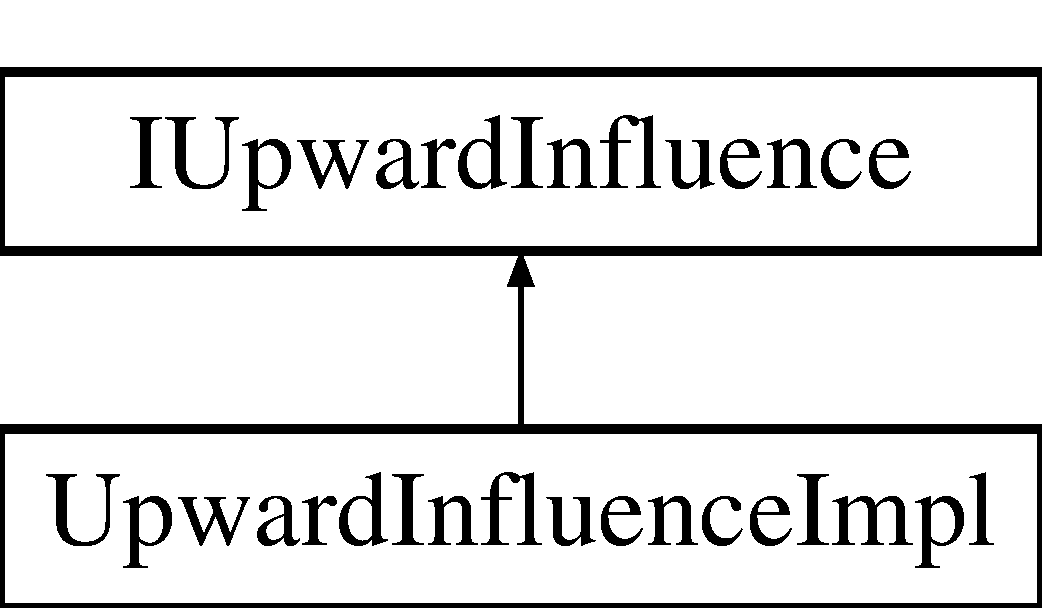
\includegraphics[height=2.000000cm]{classUpwardInfluenceImpl}
\end{center}
\end{figure}
\subsection*{Public Member Functions}
\begin{DoxyCompactItemize}
\item 
{\bfseries Upward\+Influence\+Impl} (\hyperlink{classNode}{Node} $\ast$node)\hypertarget{classUpwardInfluenceImpl_a33c1dc6e1d3cd99e7fab6c9cbc797fcf}{}\label{classUpwardInfluenceImpl_a33c1dc6e1d3cd99e7fab6c9cbc797fcf}

\item 
void {\bfseries calculate\+Upward\+Influence} ()\hypertarget{classUpwardInfluenceImpl_a30b4639db2644244553b54300f84a12c}{}\label{classUpwardInfluenceImpl_a30b4639db2644244553b54300f84a12c}

\end{DoxyCompactItemize}
\subsection*{Additional Inherited Members}


The documentation for this class was generated from the following files\+:\begin{DoxyCompactItemize}
\item 
/home/mate/\+Documents/\+Programming/\+Research/\+Multilayer\+Network\+Model/\+Multilayer\+Network\+Model/src/core/include/Upward\+Influence\+Impl.\+hh\item 
/home/mate/\+Documents/\+Programming/\+Research/\+Multilayer\+Network\+Model/\+Multilayer\+Network\+Model/src/core/src/Upward\+Influence\+Impl.\+cc\end{DoxyCompactItemize}

\hypertarget{structUTF16}{}\section{U\+T\+F16$<$ Char\+Type $>$ Struct Template Reference}
\label{structUTF16}\index{U\+T\+F16$<$ Char\+Type $>$@{U\+T\+F16$<$ Char\+Type $>$}}


U\+T\+F-\/16 encoding.  




{\ttfamily \#include $<$encodings.\+h$>$}

Inheritance diagram for U\+T\+F16$<$ Char\+Type $>$\+:\begin{figure}[H]
\begin{center}
\leavevmode
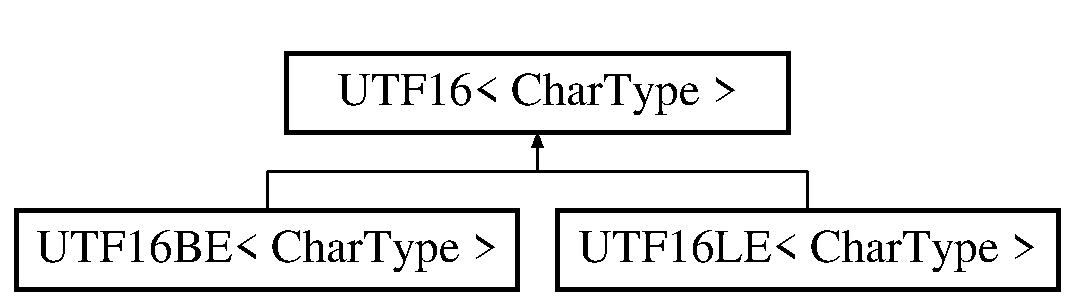
\includegraphics[height=2.000000cm]{structUTF16}
\end{center}
\end{figure}
\subsection*{Public Types}
\begin{DoxyCompactItemize}
\item 
enum \{ {\bfseries support\+Unicode} = 1
 \}\hypertarget{structUTF16_a286def80fa945e4d43d52fd398f981da}{}\label{structUTF16_a286def80fa945e4d43d52fd398f981da}

\item 
typedef Char\+Type {\bfseries Ch}\hypertarget{structUTF16_a811680d50447c98be4fd94c0a27504bb}{}\label{structUTF16_a811680d50447c98be4fd94c0a27504bb}

\end{DoxyCompactItemize}
\subsection*{Public Member Functions}
\begin{DoxyCompactItemize}
\item 
{\bfseries R\+A\+P\+I\+D\+J\+S\+O\+N\+\_\+\+S\+T\+A\+T\+I\+C\+\_\+\+A\+S\+S\+E\+RT} (sizeof(Ch) $>$=2)\hypertarget{structUTF16_a04aeeefa5dcba7c5156bc78a5c1f1557}{}\label{structUTF16_a04aeeefa5dcba7c5156bc78a5c1f1557}

\end{DoxyCompactItemize}
\subsection*{Static Public Member Functions}
\begin{DoxyCompactItemize}
\item 
{\footnotesize template$<$typename Output\+Stream $>$ }\\static void {\bfseries Encode} (Output\+Stream \&os, unsigned codepoint)\hypertarget{structUTF16_a9d8ded01244e30d037c4afa10ee2b30e}{}\label{structUTF16_a9d8ded01244e30d037c4afa10ee2b30e}

\item 
{\footnotesize template$<$typename Output\+Stream $>$ }\\static void {\bfseries Encode\+Unsafe} (Output\+Stream \&os, unsigned codepoint)\hypertarget{structUTF16_aa67661e756c273871b574e7133b7fc63}{}\label{structUTF16_aa67661e756c273871b574e7133b7fc63}

\item 
{\footnotesize template$<$typename Input\+Stream $>$ }\\static bool {\bfseries Decode} (Input\+Stream \&is, unsigned $\ast$codepoint)\hypertarget{structUTF16_a124c79dfd9f9b4c3fb65bd55ba17b4be}{}\label{structUTF16_a124c79dfd9f9b4c3fb65bd55ba17b4be}

\item 
{\footnotesize template$<$typename Input\+Stream , typename Output\+Stream $>$ }\\static bool {\bfseries Validate} (Input\+Stream \&is, Output\+Stream \&os)\hypertarget{structUTF16_a7516184ed5dce10c0e7895bec124d97d}{}\label{structUTF16_a7516184ed5dce10c0e7895bec124d97d}

\end{DoxyCompactItemize}


\subsection{Detailed Description}
\subsubsection*{template$<$typename Char\+Type = wchar\+\_\+t$>$\\*
struct U\+T\+F16$<$ Char\+Type $>$}

U\+T\+F-\/16 encoding. 

\href{http://en.wikipedia.org/wiki/UTF-16}{\tt http\+://en.\+wikipedia.\+org/wiki/\+U\+T\+F-\/16} \href{http://tools.ietf.org/html/rfc2781}{\tt http\+://tools.\+ietf.\+org/html/rfc2781} 
\begin{DoxyTemplParams}{Template Parameters}
{\em Char\+Type} & Type for storing 16-\/bit U\+T\+F-\/16 data. Default is wchar\+\_\+t. C++11 may use char16\+\_\+t instead. \\
\hline
\end{DoxyTemplParams}
\begin{DoxyNote}{Note}
implements Encoding concept

For in-\/memory access, no need to concern endianness. The code units and code points are represented by C\+PU\textquotesingle{}s endianness. For streaming, use \hyperlink{structUTF16LE}{U\+T\+F16\+LE} and \hyperlink{structUTF16BE}{U\+T\+F16\+BE}, which handle endianness. 
\end{DoxyNote}


The documentation for this struct was generated from the following file\+:\begin{DoxyCompactItemize}
\item 
/home/mate/\+Documents/\+Programming/\+Research/\+Multilayer\+Network\+Model/\+Multilayer\+Network\+Model/sources/external/rapidjson/encodings.\+h\end{DoxyCompactItemize}

\hypertarget{structUTF16BE}{}\section{U\+T\+F16\+BE$<$ Char\+Type $>$ Struct Template Reference}
\label{structUTF16BE}\index{U\+T\+F16\+B\+E$<$ Char\+Type $>$@{U\+T\+F16\+B\+E$<$ Char\+Type $>$}}


U\+T\+F-\/16 big endian encoding.  




{\ttfamily \#include $<$encodings.\+h$>$}

Inheritance diagram for U\+T\+F16\+BE$<$ Char\+Type $>$\+:\begin{figure}[H]
\begin{center}
\leavevmode
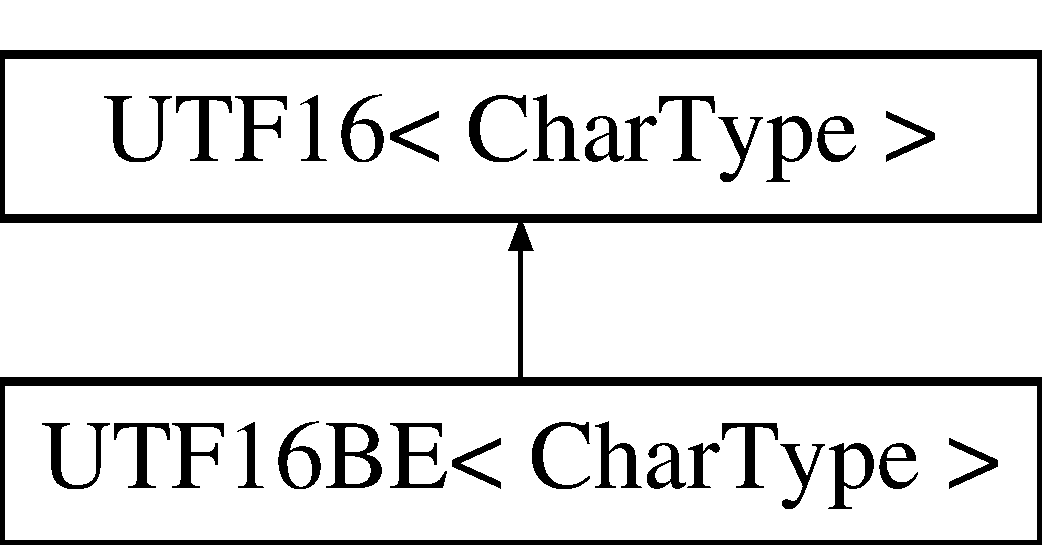
\includegraphics[height=2.000000cm]{structUTF16BE}
\end{center}
\end{figure}
\subsection*{Static Public Member Functions}
\begin{DoxyCompactItemize}
\item 
{\footnotesize template$<$typename Input\+Byte\+Stream $>$ }\\static Char\+Type {\bfseries Take\+B\+OM} (Input\+Byte\+Stream \&is)\hypertarget{structUTF16BE_a5d5184a373149c69b4b8baf8507f9591}{}\label{structUTF16BE_a5d5184a373149c69b4b8baf8507f9591}

\item 
{\footnotesize template$<$typename Input\+Byte\+Stream $>$ }\\static Char\+Type {\bfseries Take} (Input\+Byte\+Stream \&is)\hypertarget{structUTF16BE_a671ca76d54f45aa5f62eb86c4e69738a}{}\label{structUTF16BE_a671ca76d54f45aa5f62eb86c4e69738a}

\item 
{\footnotesize template$<$typename Output\+Byte\+Stream $>$ }\\static void {\bfseries Put\+B\+OM} (Output\+Byte\+Stream \&os)\hypertarget{structUTF16BE_ae109dda1ad7955049589885ea5a13652}{}\label{structUTF16BE_ae109dda1ad7955049589885ea5a13652}

\item 
{\footnotesize template$<$typename Output\+Byte\+Stream $>$ }\\static void {\bfseries Put} (Output\+Byte\+Stream \&os, Char\+Type c)\hypertarget{structUTF16BE_ab0f964c3ec9ac6cc47f2875ae112dbfe}{}\label{structUTF16BE_ab0f964c3ec9ac6cc47f2875ae112dbfe}

\end{DoxyCompactItemize}
\subsection*{Additional Inherited Members}


\subsection{Detailed Description}
\subsubsection*{template$<$typename Char\+Type = wchar\+\_\+t$>$\\*
struct U\+T\+F16\+B\+E$<$ Char\+Type $>$}

U\+T\+F-\/16 big endian encoding. 

The documentation for this struct was generated from the following file\+:\begin{DoxyCompactItemize}
\item 
/home/mate/\+Documents/\+Programming/\+Research/\+Multilayer\+Network\+Model/\+Multilayer\+Network\+Model/sources/external/rapidjson/encodings.\+h\end{DoxyCompactItemize}

\hypertarget{structUTF16LE}{}\section{U\+T\+F16\+LE$<$ Char\+Type $>$ Struct Template Reference}
\label{structUTF16LE}\index{U\+T\+F16\+L\+E$<$ Char\+Type $>$@{U\+T\+F16\+L\+E$<$ Char\+Type $>$}}


U\+T\+F-\/16 little endian encoding.  




{\ttfamily \#include $<$encodings.\+h$>$}

Inheritance diagram for U\+T\+F16\+LE$<$ Char\+Type $>$\+:\begin{figure}[H]
\begin{center}
\leavevmode
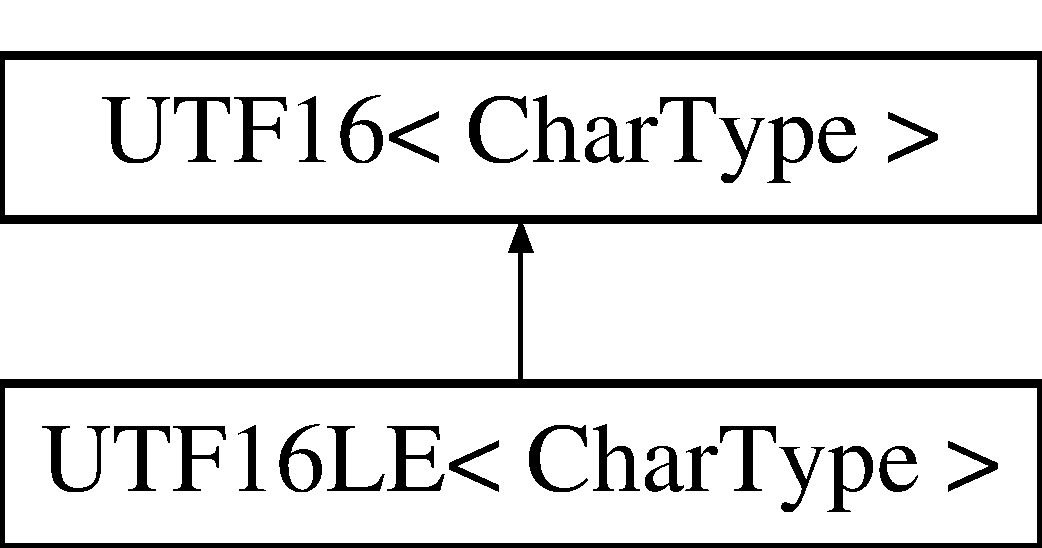
\includegraphics[height=2.000000cm]{structUTF16LE}
\end{center}
\end{figure}
\subsection*{Static Public Member Functions}
\begin{DoxyCompactItemize}
\item 
{\footnotesize template$<$typename Input\+Byte\+Stream $>$ }\\static Char\+Type {\bfseries Take\+B\+OM} (Input\+Byte\+Stream \&is)\hypertarget{structUTF16LE_ab1d5f43903815155796733f76b21deea}{}\label{structUTF16LE_ab1d5f43903815155796733f76b21deea}

\item 
{\footnotesize template$<$typename Input\+Byte\+Stream $>$ }\\static Char\+Type {\bfseries Take} (Input\+Byte\+Stream \&is)\hypertarget{structUTF16LE_a5927b3d75ff9ce02056d827c14bd0160}{}\label{structUTF16LE_a5927b3d75ff9ce02056d827c14bd0160}

\item 
{\footnotesize template$<$typename Output\+Byte\+Stream $>$ }\\static void {\bfseries Put\+B\+OM} (Output\+Byte\+Stream \&os)\hypertarget{structUTF16LE_a6bfd05f8cac35c1594c7fce47009f198}{}\label{structUTF16LE_a6bfd05f8cac35c1594c7fce47009f198}

\item 
{\footnotesize template$<$typename Output\+Byte\+Stream $>$ }\\static void {\bfseries Put} (Output\+Byte\+Stream \&os, Char\+Type c)\hypertarget{structUTF16LE_ac018cc43a1dba5a6ca232bd9a257072c}{}\label{structUTF16LE_ac018cc43a1dba5a6ca232bd9a257072c}

\end{DoxyCompactItemize}
\subsection*{Additional Inherited Members}


\subsection{Detailed Description}
\subsubsection*{template$<$typename Char\+Type = wchar\+\_\+t$>$\\*
struct U\+T\+F16\+L\+E$<$ Char\+Type $>$}

U\+T\+F-\/16 little endian encoding. 

The documentation for this struct was generated from the following file\+:\begin{DoxyCompactItemize}
\item 
/home/mate/\+Documents/\+Programming/\+Research/\+Multilayer\+Network\+Model/\+Multilayer\+Network\+Model/sources/external/rapidjson/encodings.\+h\end{DoxyCompactItemize}

\hypertarget{structUTF32}{}\section{U\+T\+F32$<$ Char\+Type $>$ Struct Template Reference}
\label{structUTF32}\index{U\+T\+F32$<$ Char\+Type $>$@{U\+T\+F32$<$ Char\+Type $>$}}


U\+T\+F-\/32 encoding.  




{\ttfamily \#include $<$encodings.\+h$>$}

Inheritance diagram for U\+T\+F32$<$ Char\+Type $>$\+:\begin{figure}[H]
\begin{center}
\leavevmode
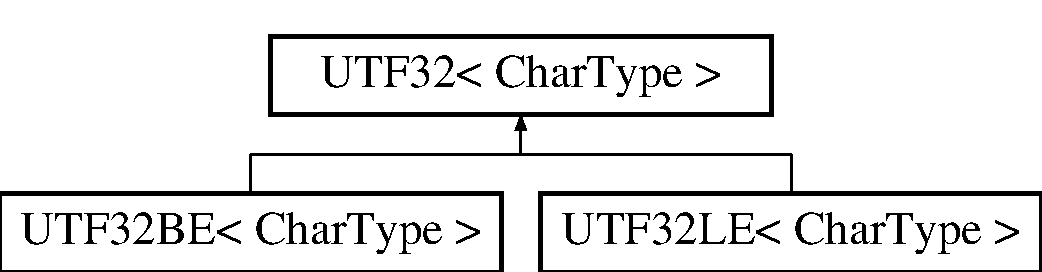
\includegraphics[height=2.000000cm]{structUTF32}
\end{center}
\end{figure}
\subsection*{Public Types}
\begin{DoxyCompactItemize}
\item 
enum \{ {\bfseries support\+Unicode} = 1
 \}\hypertarget{structUTF32_abe791c52b9d1305aacf92ddc15c11ab4}{}\label{structUTF32_abe791c52b9d1305aacf92ddc15c11ab4}

\item 
typedef Char\+Type {\bfseries Ch}\hypertarget{structUTF32_ab4502672d56436e730ca5f647bb52be9}{}\label{structUTF32_ab4502672d56436e730ca5f647bb52be9}

\end{DoxyCompactItemize}
\subsection*{Public Member Functions}
\begin{DoxyCompactItemize}
\item 
{\bfseries R\+A\+P\+I\+D\+J\+S\+O\+N\+\_\+\+S\+T\+A\+T\+I\+C\+\_\+\+A\+S\+S\+E\+RT} (sizeof(Ch) $>$=4)\hypertarget{structUTF32_aae11b766f799d311679d59e9f7077f83}{}\label{structUTF32_aae11b766f799d311679d59e9f7077f83}

\end{DoxyCompactItemize}
\subsection*{Static Public Member Functions}
\begin{DoxyCompactItemize}
\item 
{\footnotesize template$<$typename Output\+Stream $>$ }\\static void {\bfseries Encode} (Output\+Stream \&os, unsigned codepoint)\hypertarget{structUTF32_a511d1b09672ce535085895a28d8c2f13}{}\label{structUTF32_a511d1b09672ce535085895a28d8c2f13}

\item 
{\footnotesize template$<$typename Output\+Stream $>$ }\\static void {\bfseries Encode\+Unsafe} (Output\+Stream \&os, unsigned codepoint)\hypertarget{structUTF32_ae50dd8dff92c36ee184c6d4eccb1961e}{}\label{structUTF32_ae50dd8dff92c36ee184c6d4eccb1961e}

\item 
{\footnotesize template$<$typename Input\+Stream $>$ }\\static bool {\bfseries Decode} (Input\+Stream \&is, unsigned $\ast$codepoint)\hypertarget{structUTF32_a6e7258a5e982e101345dffdc355e9b53}{}\label{structUTF32_a6e7258a5e982e101345dffdc355e9b53}

\item 
{\footnotesize template$<$typename Input\+Stream , typename Output\+Stream $>$ }\\static bool {\bfseries Validate} (Input\+Stream \&is, Output\+Stream \&os)\hypertarget{structUTF32_a71336fb0546b3079e01bbd51d2fa2e45}{}\label{structUTF32_a71336fb0546b3079e01bbd51d2fa2e45}

\end{DoxyCompactItemize}


\subsection{Detailed Description}
\subsubsection*{template$<$typename Char\+Type = unsigned$>$\\*
struct U\+T\+F32$<$ Char\+Type $>$}

U\+T\+F-\/32 encoding. 

\href{http://en.wikipedia.org/wiki/UTF-32}{\tt http\+://en.\+wikipedia.\+org/wiki/\+U\+T\+F-\/32} 
\begin{DoxyTemplParams}{Template Parameters}
{\em Char\+Type} & Type for storing 32-\/bit U\+T\+F-\/32 data. Default is unsigned. C++11 may use char32\+\_\+t instead. \\
\hline
\end{DoxyTemplParams}
\begin{DoxyNote}{Note}
implements Encoding concept

For in-\/memory access, no need to concern endianness. The code units and code points are represented by C\+PU\textquotesingle{}s endianness. For streaming, use \hyperlink{structUTF32LE}{U\+T\+F32\+LE} and \hyperlink{structUTF32BE}{U\+T\+F32\+BE}, which handle endianness. 
\end{DoxyNote}


The documentation for this struct was generated from the following file\+:\begin{DoxyCompactItemize}
\item 
/home/mate/\+Documents/\+Programming/\+Research/\+Multilayer\+Network\+Model/\+Multilayer\+Network\+Model/src/external/rapidjson/encodings.\+h\end{DoxyCompactItemize}

\hypertarget{structUTF32BE}{}\section{U\+T\+F32\+BE$<$ Char\+Type $>$ Struct Template Reference}
\label{structUTF32BE}\index{U\+T\+F32\+B\+E$<$ Char\+Type $>$@{U\+T\+F32\+B\+E$<$ Char\+Type $>$}}


U\+T\+F-\/32 big endian encoding.  




{\ttfamily \#include $<$encodings.\+h$>$}

Inheritance diagram for U\+T\+F32\+BE$<$ Char\+Type $>$\+:\begin{figure}[H]
\begin{center}
\leavevmode
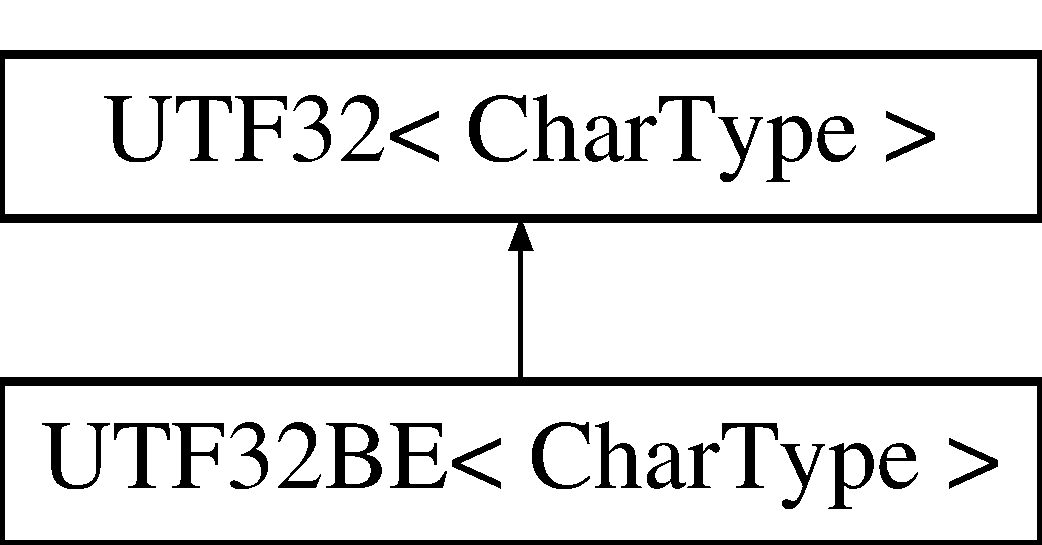
\includegraphics[height=2.000000cm]{structUTF32BE}
\end{center}
\end{figure}
\subsection*{Static Public Member Functions}
\begin{DoxyCompactItemize}
\item 
{\footnotesize template$<$typename Input\+Byte\+Stream $>$ }\\static Char\+Type {\bfseries Take\+B\+OM} (Input\+Byte\+Stream \&is)\hypertarget{structUTF32BE_a07d228f51ad43ef83af2529ca4bd1181}{}\label{structUTF32BE_a07d228f51ad43ef83af2529ca4bd1181}

\item 
{\footnotesize template$<$typename Input\+Byte\+Stream $>$ }\\static Char\+Type {\bfseries Take} (Input\+Byte\+Stream \&is)\hypertarget{structUTF32BE_ace3086ece3b13417c758b5abcf3016c8}{}\label{structUTF32BE_ace3086ece3b13417c758b5abcf3016c8}

\item 
{\footnotesize template$<$typename Output\+Byte\+Stream $>$ }\\static void {\bfseries Put\+B\+OM} (Output\+Byte\+Stream \&os)\hypertarget{structUTF32BE_a8b1a216dd267ff06a9000cbe593ebd24}{}\label{structUTF32BE_a8b1a216dd267ff06a9000cbe593ebd24}

\item 
{\footnotesize template$<$typename Output\+Byte\+Stream $>$ }\\static void {\bfseries Put} (Output\+Byte\+Stream \&os, Char\+Type c)\hypertarget{structUTF32BE_ad270b8b016d477f7f7354df535fa28c5}{}\label{structUTF32BE_ad270b8b016d477f7f7354df535fa28c5}

\end{DoxyCompactItemize}
\subsection*{Additional Inherited Members}


\subsection{Detailed Description}
\subsubsection*{template$<$typename Char\+Type = unsigned$>$\\*
struct U\+T\+F32\+B\+E$<$ Char\+Type $>$}

U\+T\+F-\/32 big endian encoding. 

The documentation for this struct was generated from the following file\+:\begin{DoxyCompactItemize}
\item 
/home/mate/\+Documents/\+Programming/\+Research/\+Multilayer\+Network\+Model/\+Multilayer\+Network\+Model/src/external/rapidjson/encodings.\+h\end{DoxyCompactItemize}

\hypertarget{structUTF32LE}{}\section{U\+T\+F32\+LE$<$ Char\+Type $>$ Struct Template Reference}
\label{structUTF32LE}\index{U\+T\+F32\+L\+E$<$ Char\+Type $>$@{U\+T\+F32\+L\+E$<$ Char\+Type $>$}}


U\+T\+F-\/32 little endian enocoding.  




{\ttfamily \#include $<$encodings.\+h$>$}

Inheritance diagram for U\+T\+F32\+LE$<$ Char\+Type $>$\+:\begin{figure}[H]
\begin{center}
\leavevmode
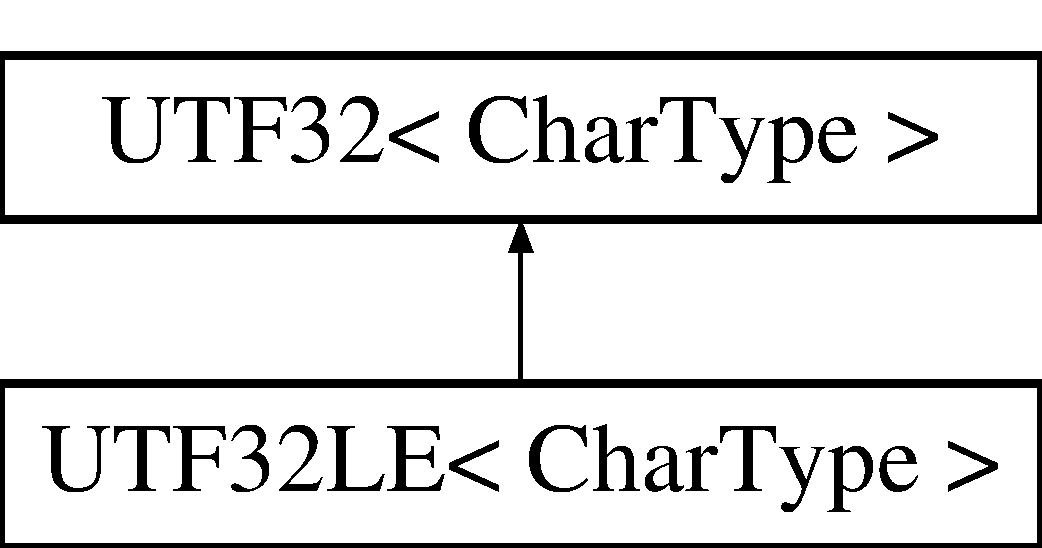
\includegraphics[height=2.000000cm]{structUTF32LE}
\end{center}
\end{figure}
\subsection*{Static Public Member Functions}
\begin{DoxyCompactItemize}
\item 
{\footnotesize template$<$typename Input\+Byte\+Stream $>$ }\\static Char\+Type {\bfseries Take\+B\+OM} (Input\+Byte\+Stream \&is)\hypertarget{structUTF32LE_a8729612b0a8b1126c61c4f8f8c34410e}{}\label{structUTF32LE_a8729612b0a8b1126c61c4f8f8c34410e}

\item 
{\footnotesize template$<$typename Input\+Byte\+Stream $>$ }\\static Char\+Type {\bfseries Take} (Input\+Byte\+Stream \&is)\hypertarget{structUTF32LE_ad13967549811be12897362bb37b2c819}{}\label{structUTF32LE_ad13967549811be12897362bb37b2c819}

\item 
{\footnotesize template$<$typename Output\+Byte\+Stream $>$ }\\static void {\bfseries Put\+B\+OM} (Output\+Byte\+Stream \&os)\hypertarget{structUTF32LE_accd97d45e55746c900dab356605825be}{}\label{structUTF32LE_accd97d45e55746c900dab356605825be}

\item 
{\footnotesize template$<$typename Output\+Byte\+Stream $>$ }\\static void {\bfseries Put} (Output\+Byte\+Stream \&os, Char\+Type c)\hypertarget{structUTF32LE_a61bb50e7fba27e3fe28a9f30eb366193}{}\label{structUTF32LE_a61bb50e7fba27e3fe28a9f30eb366193}

\end{DoxyCompactItemize}
\subsection*{Additional Inherited Members}


\subsection{Detailed Description}
\subsubsection*{template$<$typename Char\+Type = unsigned$>$\\*
struct U\+T\+F32\+L\+E$<$ Char\+Type $>$}

U\+T\+F-\/32 little endian enocoding. 

The documentation for this struct was generated from the following file\+:\begin{DoxyCompactItemize}
\item 
/home/mate/\+Documents/\+Programming/\+Research/\+Multilayer\+Network\+Model/\+Multilayer\+Network\+Model/sources/external/rapidjson/encodings.\+h\end{DoxyCompactItemize}

\hypertarget{structUTF8}{}\section{U\+T\+F8$<$ Char\+Type $>$ Struct Template Reference}
\label{structUTF8}\index{U\+T\+F8$<$ Char\+Type $>$@{U\+T\+F8$<$ Char\+Type $>$}}


U\+T\+F-\/8 encoding.  




{\ttfamily \#include $<$encodings.\+h$>$}

\subsection*{Public Types}
\begin{DoxyCompactItemize}
\item 
enum \{ {\bfseries support\+Unicode} = 1
 \}\hypertarget{structUTF8_a6d7cd5f1f72db45d041344c35f47da74}{}\label{structUTF8_a6d7cd5f1f72db45d041344c35f47da74}

\item 
typedef Char\+Type {\bfseries Ch}\hypertarget{structUTF8_a8e78c8113f3660178d8121b7d3e55890}{}\label{structUTF8_a8e78c8113f3660178d8121b7d3e55890}

\end{DoxyCompactItemize}
\subsection*{Static Public Member Functions}
\begin{DoxyCompactItemize}
\item 
{\footnotesize template$<$typename Output\+Stream $>$ }\\static void {\bfseries Encode} (Output\+Stream \&os, unsigned codepoint)\hypertarget{structUTF8_af286ed19ca60d261a9b11b65bee1298b}{}\label{structUTF8_af286ed19ca60d261a9b11b65bee1298b}

\item 
{\footnotesize template$<$typename Output\+Stream $>$ }\\static void {\bfseries Encode\+Unsafe} (Output\+Stream \&os, unsigned codepoint)\hypertarget{structUTF8_aac6bdaf03c114265384b2ae3e425e7a8}{}\label{structUTF8_aac6bdaf03c114265384b2ae3e425e7a8}

\item 
{\footnotesize template$<$typename Input\+Stream $>$ }\\static bool {\bfseries Decode} (Input\+Stream \&is, unsigned $\ast$codepoint)\hypertarget{structUTF8_a17c6badb31acf4f784111c886737fb17}{}\label{structUTF8_a17c6badb31acf4f784111c886737fb17}

\item 
{\footnotesize template$<$typename Input\+Stream , typename Output\+Stream $>$ }\\static bool {\bfseries Validate} (Input\+Stream \&is, Output\+Stream \&os)\hypertarget{structUTF8_a9e2e7e37d819baeb5e643654c6e61e33}{}\label{structUTF8_a9e2e7e37d819baeb5e643654c6e61e33}

\item 
static unsigned char {\bfseries Get\+Range} (unsigned char c)\hypertarget{structUTF8_ac06bbf38df41adb0c7b9eaa93f85cc38}{}\label{structUTF8_ac06bbf38df41adb0c7b9eaa93f85cc38}

\item 
{\footnotesize template$<$typename Input\+Byte\+Stream $>$ }\\static Char\+Type {\bfseries Take\+B\+OM} (Input\+Byte\+Stream \&is)\hypertarget{structUTF8_a1b2359d6ea50ae32fefc9b28e9878a31}{}\label{structUTF8_a1b2359d6ea50ae32fefc9b28e9878a31}

\item 
{\footnotesize template$<$typename Input\+Byte\+Stream $>$ }\\static Ch {\bfseries Take} (Input\+Byte\+Stream \&is)\hypertarget{structUTF8_a5b2561a5031c8a699e593cd51b2c6864}{}\label{structUTF8_a5b2561a5031c8a699e593cd51b2c6864}

\item 
{\footnotesize template$<$typename Output\+Byte\+Stream $>$ }\\static void {\bfseries Put\+B\+OM} (Output\+Byte\+Stream \&os)\hypertarget{structUTF8_a6b171e5f0662ad81d498875bbdbc536a}{}\label{structUTF8_a6b171e5f0662ad81d498875bbdbc536a}

\item 
{\footnotesize template$<$typename Output\+Byte\+Stream $>$ }\\static void {\bfseries Put} (Output\+Byte\+Stream \&os, Ch c)\hypertarget{structUTF8_ab24c23227413798e9be28a21eb26fe51}{}\label{structUTF8_ab24c23227413798e9be28a21eb26fe51}

\end{DoxyCompactItemize}


\subsection{Detailed Description}
\subsubsection*{template$<$typename Char\+Type = char$>$\\*
struct U\+T\+F8$<$ Char\+Type $>$}

U\+T\+F-\/8 encoding. 

\href{http://en.wikipedia.org/wiki/UTF-8}{\tt http\+://en.\+wikipedia.\+org/wiki/\+U\+T\+F-\/8} \href{http://tools.ietf.org/html/rfc3629}{\tt http\+://tools.\+ietf.\+org/html/rfc3629} 
\begin{DoxyTemplParams}{Template Parameters}
{\em Char\+Type} & Code unit for storing 8-\/bit U\+T\+F-\/8 data. Default is char. \\
\hline
\end{DoxyTemplParams}
\begin{DoxyNote}{Note}
implements Encoding concept 
\end{DoxyNote}


The documentation for this struct was generated from the following file\+:\begin{DoxyCompactItemize}
\item 
/home/mate/\+Documents/\+Programming/\+Research/\+Multilayer\+Network\+Model/\+Multilayer\+Network\+Model/sources/external/rapidjson/encodings.\+h\end{DoxyCompactItemize}

\hypertarget{structEquationParser_1_1variant}{}\section{Equation\+Parser\+:\+:variant$<$ S $>$ Struct Template Reference}
\label{structEquationParser_1_1variant}\index{Equation\+Parser\+::variant$<$ S $>$@{Equation\+Parser\+::variant$<$ S $>$}}


{\ttfamily \#include $<$parser.\+hpp$>$}

\subsection*{Public Types}
\begin{DoxyCompactItemize}
\item 
typedef \hyperlink{structEquationParser_1_1variant}{variant}$<$ S $>$ \hyperlink{structEquationParser_1_1variant_aa17a8f334ad949693cf8f6a8197092df}{self\+\_\+type}\hypertarget{structEquationParser_1_1variant_aa17a8f334ad949693cf8f6a8197092df}{}\label{structEquationParser_1_1variant_aa17a8f334ad949693cf8f6a8197092df}

\begin{DoxyCompactList}\small\item\em Type of $\ast$this. \end{DoxyCompactList}\end{DoxyCompactItemize}
\subsection*{Public Member Functions}
\begin{DoxyCompactItemize}
\item 
\hyperlink{structEquationParser_1_1variant_a660b1678a9ba872275b4ddf9a28d871a}{variant} ()\hypertarget{structEquationParser_1_1variant_a660b1678a9ba872275b4ddf9a28d871a}{}\label{structEquationParser_1_1variant_a660b1678a9ba872275b4ddf9a28d871a}

\begin{DoxyCompactList}\small\item\em Empty construction. \end{DoxyCompactList}\item 
{\footnotesize template$<$typename T $>$ }\\\hyperlink{structEquationParser_1_1variant_aff2dbf78ab3b00b4b3f184929c8c0472}{variant} (const T \&t)\hypertarget{structEquationParser_1_1variant_aff2dbf78ab3b00b4b3f184929c8c0472}{}\label{structEquationParser_1_1variant_aff2dbf78ab3b00b4b3f184929c8c0472}

\begin{DoxyCompactList}\small\item\em Construct and fill. \end{DoxyCompactList}\item 
\hyperlink{structEquationParser_1_1variant_a0c86b8e89ec8f00a8d9e3e9e7538567b}{$\sim$variant} ()\hypertarget{structEquationParser_1_1variant_a0c86b8e89ec8f00a8d9e3e9e7538567b}{}\label{structEquationParser_1_1variant_a0c86b8e89ec8f00a8d9e3e9e7538567b}

\begin{DoxyCompactList}\small\item\em Destruction, allowed only if empty. \end{DoxyCompactList}\item 
{\footnotesize template$<$typename T $>$ }\\T \& \hyperlink{structEquationParser_1_1variant_a488e3c6e9321a397a505bf2e2d948fb7}{build} ()\hypertarget{structEquationParser_1_1variant_a488e3c6e9321a397a505bf2e2d948fb7}{}\label{structEquationParser_1_1variant_a488e3c6e9321a397a505bf2e2d948fb7}

\begin{DoxyCompactList}\small\item\em Instantiate an empty {\itshape T} in here. \end{DoxyCompactList}\item 
{\footnotesize template$<$typename T $>$ }\\T \& \hyperlink{structEquationParser_1_1variant_a2cb4ec9e01e9ad7d09f8cb487353f6db}{build} (const T \&t)\hypertarget{structEquationParser_1_1variant_a2cb4ec9e01e9ad7d09f8cb487353f6db}{}\label{structEquationParser_1_1variant_a2cb4ec9e01e9ad7d09f8cb487353f6db}

\begin{DoxyCompactList}\small\item\em Instantiate a {\itshape T} in here from {\itshape t}. \end{DoxyCompactList}\item 
{\footnotesize template$<$typename T $>$ }\\T \& \hyperlink{structEquationParser_1_1variant_a42b14ef536da4960050a0db0d539dd5f}{as} ()\hypertarget{structEquationParser_1_1variant_a42b14ef536da4960050a0db0d539dd5f}{}\label{structEquationParser_1_1variant_a42b14ef536da4960050a0db0d539dd5f}

\begin{DoxyCompactList}\small\item\em Accessor to a built {\itshape T}. \end{DoxyCompactList}\item 
{\footnotesize template$<$typename T $>$ }\\const T \& \hyperlink{structEquationParser_1_1variant_af0e6dea306d2be91b6e12de6dd968e3b}{as} () const \hypertarget{structEquationParser_1_1variant_af0e6dea306d2be91b6e12de6dd968e3b}{}\label{structEquationParser_1_1variant_af0e6dea306d2be91b6e12de6dd968e3b}

\begin{DoxyCompactList}\small\item\em Const accessor to a built {\itshape T} (for printer). \end{DoxyCompactList}\item 
{\footnotesize template$<$typename T $>$ }\\void \hyperlink{structEquationParser_1_1variant_a7f5bd11f1d463f569efa8c2ca096f13e}{swap} (\hyperlink{structEquationParser_1_1variant_aa17a8f334ad949693cf8f6a8197092df}{self\+\_\+type} \&other)
\item 
{\footnotesize template$<$typename T $>$ }\\void \hyperlink{structEquationParser_1_1variant_ab995b43f5da5ebbf8e22b478610cc665}{move} (\hyperlink{structEquationParser_1_1variant_aa17a8f334ad949693cf8f6a8197092df}{self\+\_\+type} \&other)
\item 
{\footnotesize template$<$typename T $>$ }\\void \hyperlink{structEquationParser_1_1variant_a6a418207d721caaa7cb795f64da7769a}{copy} (const \hyperlink{structEquationParser_1_1variant_aa17a8f334ad949693cf8f6a8197092df}{self\+\_\+type} \&other)\hypertarget{structEquationParser_1_1variant_a6a418207d721caaa7cb795f64da7769a}{}\label{structEquationParser_1_1variant_a6a418207d721caaa7cb795f64da7769a}

\begin{DoxyCompactList}\small\item\em Copy the content of {\itshape other} to this. \end{DoxyCompactList}\item 
{\footnotesize template$<$typename T $>$ }\\void \hyperlink{structEquationParser_1_1variant_aba79dc64be387f0bbcbc13770d484568}{destroy} ()\hypertarget{structEquationParser_1_1variant_aba79dc64be387f0bbcbc13770d484568}{}\label{structEquationParser_1_1variant_aba79dc64be387f0bbcbc13770d484568}

\begin{DoxyCompactList}\small\item\em Destroy the stored {\itshape T}. \end{DoxyCompactList}\end{DoxyCompactItemize}


\subsection{Detailed Description}
\subsubsection*{template$<$size\+\_\+t S$>$\\*
struct Equation\+Parser\+::variant$<$ S $>$}

A char\mbox{[}S\mbox{]} buffer to store and retrieve objects.

Sort of a variant, but does not keep track of the nature of the stored data, since that knowledge is available via the current state. 

\subsection{Member Function Documentation}
\index{Equation\+Parser\+::variant@{Equation\+Parser\+::variant}!move@{move}}
\index{move@{move}!Equation\+Parser\+::variant@{Equation\+Parser\+::variant}}
\subsubsection[{\texorpdfstring{move(self\+\_\+type \&other)}{move(self_type &other)}}]{\setlength{\rightskip}{0pt plus 5cm}template$<$size\+\_\+t S$>$ template$<$typename T $>$ void {\bf Equation\+Parser\+::variant}$<$ S $>$\+::move (
\begin{DoxyParamCaption}
\item[{{\bf self\+\_\+type} \&}]{other}
\end{DoxyParamCaption}
)\hspace{0.3cm}{\ttfamily [inline]}}\hypertarget{structEquationParser_1_1variant_ab995b43f5da5ebbf8e22b478610cc665}{}\label{structEquationParser_1_1variant_ab995b43f5da5ebbf8e22b478610cc665}
Move the content of {\itshape other} to this.

Destroys {\itshape other}. \index{Equation\+Parser\+::variant@{Equation\+Parser\+::variant}!swap@{swap}}
\index{swap@{swap}!Equation\+Parser\+::variant@{Equation\+Parser\+::variant}}
\subsubsection[{\texorpdfstring{swap(self\+\_\+type \&other)}{swap(self_type &other)}}]{\setlength{\rightskip}{0pt plus 5cm}template$<$size\+\_\+t S$>$ template$<$typename T $>$ void {\bf Equation\+Parser\+::variant}$<$ S $>$\+::swap (
\begin{DoxyParamCaption}
\item[{{\bf self\+\_\+type} \&}]{other}
\end{DoxyParamCaption}
)\hspace{0.3cm}{\ttfamily [inline]}}\hypertarget{structEquationParser_1_1variant_a7f5bd11f1d463f569efa8c2ca096f13e}{}\label{structEquationParser_1_1variant_a7f5bd11f1d463f569efa8c2ca096f13e}
Swap the content with {\itshape other}, of same type.

Both variants must be built beforehand, because swapping the actual data requires reading it (with \hyperlink{structEquationParser_1_1variant_a42b14ef536da4960050a0db0d539dd5f}{as()}), and this is not possible on unconstructed variants\+: it would require some dynamic testing, which should not be the variant\textquotesingle{}s responsability. Swapping between built and (possibly) non-\/built is done with \hyperlink{structEquationParser_1_1variant_ab995b43f5da5ebbf8e22b478610cc665}{variant\+::move} (). 

The documentation for this struct was generated from the following file\+:\begin{DoxyCompactItemize}
\item 
/home/mate/\+Documents/\+Programming/\+Research/\+Multilayer\+Network\+Model/\+Multilayer\+Network\+Model/sources/parser/include/\hyperlink{parser_8hpp}{parser.\+hpp}\end{DoxyCompactItemize}

\hypertarget{classVectorField}{}\section{Vector\+Field Class Reference}
\label{classVectorField}\index{Vector\+Field@{Vector\+Field}}
\subsection*{Public Member Functions}
\begin{DoxyCompactItemize}
\item 
void {\bfseries add\+Point} (std\+::map$<$ int, double $>$ coordinate, std\+::map$<$ int, double $>$ direction)\hypertarget{classVectorField_ac72253d7b3410d3ef4ea520fded2d1f1}{}\label{classVectorField_ac72253d7b3410d3ef4ea520fded2d1f1}

\item 
std\+::vector$<$ \hyperlink{classVectorFieldPoint}{Vector\+Field\+Point} $\ast$ $>$ {\bfseries get\+Vector\+Field\+Points} ()\hypertarget{classVectorField_a79f35e239c04f89a3987f8ae70b49ef9}{}\label{classVectorField_a79f35e239c04f89a3987f8ae70b49ef9}

\item 
double {\bfseries get\+Distance\+From} (\hyperlink{classVectorField}{Vector\+Field} $\ast$vector\+Field)\hypertarget{classVectorField_a9cf9f0a60b62422a406a8530e10ed402}{}\label{classVectorField_a9cf9f0a60b62422a406a8530e10ed402}

\item 
std\+::map$<$ int, double $>$ {\bfseries get\+Direction\+For\+Coordinate} (std\+::map$<$ int, double $>$ coordinate)\hypertarget{classVectorField_ae8f028240c6b4ba60815660a887b92a4}{}\label{classVectorField_ae8f028240c6b4ba60815660a887b92a4}

\end{DoxyCompactItemize}
\subsection*{Friends}
\begin{DoxyCompactItemize}
\item 
std\+::ostream \& {\bfseries operator$<$$<$} (std\+::ostream \&os, const \hyperlink{classVectorField}{Vector\+Field} \&vector\+Field)\hypertarget{classVectorField_a305be31f220fc6801fa91592e7a08a9b}{}\label{classVectorField_a305be31f220fc6801fa91592e7a08a9b}

\end{DoxyCompactItemize}


The documentation for this class was generated from the following files\+:\begin{DoxyCompactItemize}
\item 
/home/mate/\+Documents/\+Programming/\+Research/\+Multilayer\+Network\+Model/\+Multilayer\+Network\+Model/src/core/include/Vector\+Field.\+hh\item 
/home/mate/\+Documents/\+Programming/\+Research/\+Multilayer\+Network\+Model/\+Multilayer\+Network\+Model/src/core/src/Vector\+Field.\+cc\end{DoxyCompactItemize}

\hypertarget{classVectorFieldPoint}{}\section{Vector\+Field\+Point Class Reference}
\label{classVectorFieldPoint}\index{Vector\+Field\+Point@{Vector\+Field\+Point}}
\subsection*{Public Member Functions}
\begin{DoxyCompactItemize}
\item 
{\bfseries Vector\+Field\+Point} (std\+::map$<$ int, double $>$ coordinate, std\+::map$<$ int, double $>$ direction)\hypertarget{classVectorFieldPoint_aaf7f444221b412f58e3066fb359f6ced}{}\label{classVectorFieldPoint_aaf7f444221b412f58e3066fb359f6ced}

\item 
std\+::map$<$ int, double $>$ {\bfseries get\+Coordinate} ()\hypertarget{classVectorFieldPoint_aaac572daff42e5aa46d92ffc2f681095}{}\label{classVectorFieldPoint_aaac572daff42e5aa46d92ffc2f681095}

\item 
std\+::map$<$ int, double $>$ {\bfseries get\+Direction} ()\hypertarget{classVectorFieldPoint_a185b994999d47371fad7e8156e211f28}{}\label{classVectorFieldPoint_a185b994999d47371fad7e8156e211f28}

\end{DoxyCompactItemize}
\subsection*{Friends}
\begin{DoxyCompactItemize}
\item 
std\+::ostream \& {\bfseries operator$<$$<$} (std\+::ostream \&os, const \hyperlink{classVectorFieldPoint}{Vector\+Field\+Point} \&vector\+Field\+Point)\hypertarget{classVectorFieldPoint_a0acdca72efec81baafb8b278ed2a545f}{}\label{classVectorFieldPoint_a0acdca72efec81baafb8b278ed2a545f}

\end{DoxyCompactItemize}


The documentation for this class was generated from the following file\+:\begin{DoxyCompactItemize}
\item 
/home/mate/\+Documents/\+Programming/\+Research/\+Multilayer\+Network\+Model/\+Multilayer\+Network\+Model/sources/core/\+Vector\+Field\+Reconfiguration/include/Vector\+Field\+Point.\+hh\end{DoxyCompactItemize}

\hypertarget{classVectorFieldReconfigurationImpl}{}\section{Vector\+Field\+Reconfiguration\+Impl Class Reference}
\label{classVectorFieldReconfigurationImpl}\index{Vector\+Field\+Reconfiguration\+Impl@{Vector\+Field\+Reconfiguration\+Impl}}
Inheritance diagram for Vector\+Field\+Reconfiguration\+Impl\+:\begin{figure}[H]
\begin{center}
\leavevmode
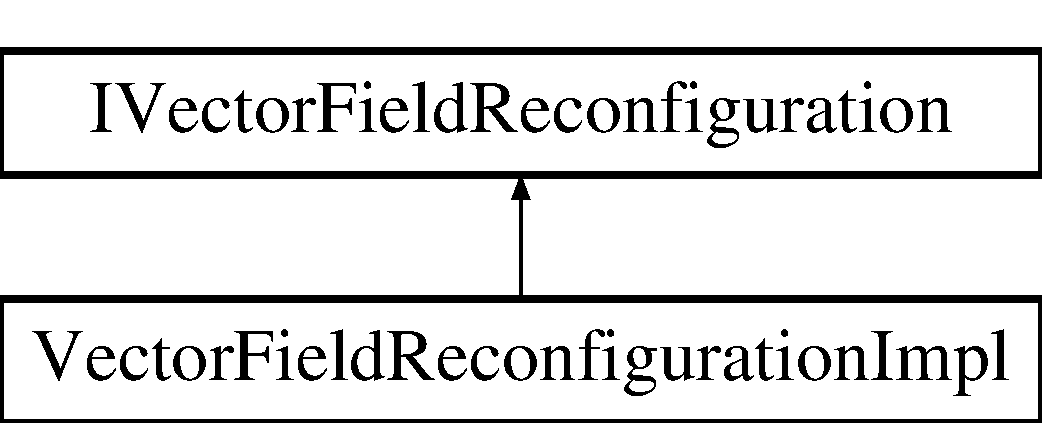
\includegraphics[height=2.000000cm]{classVectorFieldReconfigurationImpl}
\end{center}
\end{figure}
\subsection*{Public Member Functions}
\begin{DoxyCompactItemize}
\item 
{\bfseries Vector\+Field\+Reconfiguration\+Impl} (\hyperlink{classNode}{Node} $\ast$node)\hypertarget{classVectorFieldReconfigurationImpl_a42670d176dfc295f342033869defc178}{}\label{classVectorFieldReconfigurationImpl_a42670d176dfc295f342033869defc178}

\item 
void {\bfseries calculate\+Vector\+Field\+Reconfiguration} ()\hypertarget{classVectorFieldReconfigurationImpl_a2143e9fc6631fb61390e8881404891a5}{}\label{classVectorFieldReconfigurationImpl_a2143e9fc6631fb61390e8881404891a5}

\item 
void {\bfseries calculate\+Target\+Vector\+Field} (\hyperlink{classVectorField}{Vector\+Field} $\ast$target\+Vector\+Field, \hyperlink{classVectorField}{Vector\+Field} $\ast$current\+Vector\+Field, std\+::map$<$ int, double $>$ direction\+In\+Lower\+Network, std\+::map$<$ int, double $>$ direction\+In\+Higher\+Networks)\hypertarget{classVectorFieldReconfigurationImpl_aae26dcd63e8c68cfac045b90e101c522}{}\label{classVectorFieldReconfigurationImpl_aae26dcd63e8c68cfac045b90e101c522}

\item 
std\+::map$<$ int, double $>$ {\bfseries calculate\+Lower\+Network\+Direction} ()\hypertarget{classVectorFieldReconfigurationImpl_ab2746d147258dc03cf7ffbbfb0abe738}{}\label{classVectorFieldReconfigurationImpl_ab2746d147258dc03cf7ffbbfb0abe738}

\item 
std\+::map$<$ int, double $>$ {\bfseries calculate\+Higher\+Networks\+Direction} ()\hypertarget{classVectorFieldReconfigurationImpl_a2e6d7b501b830cfdbf069f8b70a75a62}{}\label{classVectorFieldReconfigurationImpl_a2e6d7b501b830cfdbf069f8b70a75a62}

\end{DoxyCompactItemize}
\subsection*{Additional Inherited Members}


The documentation for this class was generated from the following files\+:\begin{DoxyCompactItemize}
\item 
/home/mate/\+Documents/\+Programming/\+Research/\+Multilayer\+Network\+Model/\+Multilayer\+Network\+Model/src/core/include/Vector\+Field\+Reconfiguration\+Impl.\+hh\item 
/home/mate/\+Documents/\+Programming/\+Research/\+Multilayer\+Network\+Model/\+Multilayer\+Network\+Model/src/core/src/Vector\+Field\+Reconfiguration\+Impl.\+cc\end{DoxyCompactItemize}

\hypertarget{classWriter}{}\section{Writer$<$ Output\+Stream, Source\+Encoding, Target\+Encoding, Stack\+Allocator, write\+Flags $>$ Class Template Reference}
\label{classWriter}\index{Writer$<$ Output\+Stream, Source\+Encoding, Target\+Encoding, Stack\+Allocator, write\+Flags $>$@{Writer$<$ Output\+Stream, Source\+Encoding, Target\+Encoding, Stack\+Allocator, write\+Flags $>$}}


J\+S\+ON writer.  




{\ttfamily \#include $<$writer.\+h$>$}

Inheritance diagram for Writer$<$ Output\+Stream, Source\+Encoding, Target\+Encoding, Stack\+Allocator, write\+Flags $>$\+:\begin{figure}[H]
\begin{center}
\leavevmode
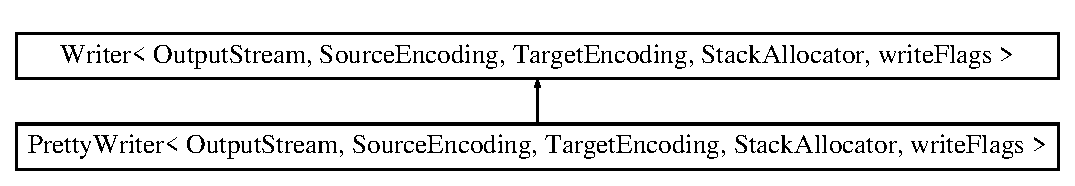
\includegraphics[height=2.000000cm]{classWriter}
\end{center}
\end{figure}
\subsection*{Classes}
\begin{DoxyCompactItemize}
\item 
struct \hyperlink{structWriter_1_1Level}{Level}
\begin{DoxyCompactList}\small\item\em Information for each nested level. \end{DoxyCompactList}\end{DoxyCompactItemize}
\subsection*{Public Types}
\begin{DoxyCompactItemize}
\item 
typedef Source\+Encoding\+::\+Ch {\bfseries Ch}\hypertarget{classWriter_ab08bff5fd2daec65f4a78779ca3d2139}{}\label{classWriter_ab08bff5fd2daec65f4a78779ca3d2139}

\end{DoxyCompactItemize}
\subsection*{Public Member Functions}
\begin{DoxyCompactItemize}
\item 
\hyperlink{classWriter_af4f54830d6927d9daf5bd53bfd134dd3}{Writer} (Output\+Stream \&os, Stack\+Allocator $\ast$stack\+Allocator=0, size\+\_\+t level\+Depth=k\+Default\+Level\+Depth)
\begin{DoxyCompactList}\small\item\em Constructor. \end{DoxyCompactList}\item 
{\bfseries Writer} (Stack\+Allocator $\ast$allocator=0, size\+\_\+t level\+Depth=k\+Default\+Level\+Depth)\hypertarget{classWriter_a7b885cea71542fc436be80eff447fb64}{}\label{classWriter_a7b885cea71542fc436be80eff447fb64}

\item 
void \hyperlink{classWriter_a8b53e8f137f7fcf694f5500711b3f58d}{Reset} (Output\+Stream \&os)
\begin{DoxyCompactList}\small\item\em Reset the writer with a new stream. \end{DoxyCompactList}\item 
bool \hyperlink{classWriter_a446cfad4b88cfd69b1b63d57989f2e76}{Is\+Complete} () const 
\begin{DoxyCompactList}\small\item\em Checks whether the output is a complete J\+S\+ON. \end{DoxyCompactList}\item 
int {\bfseries Get\+Max\+Decimal\+Places} () const \hypertarget{classWriter_abbd76fd072c7feca94ddb0a02fb6e44b}{}\label{classWriter_abbd76fd072c7feca94ddb0a02fb6e44b}

\item 
void \hyperlink{classWriter_a58e3f94dc5af1432a8eace5ba427eca7}{Set\+Max\+Decimal\+Places} (int max\+Decimal\+Places)
\begin{DoxyCompactList}\small\item\em Sets the maximum number of decimal places for double output. \end{DoxyCompactList}\item 
bool \hyperlink{classWriter_ae0d1615104e4e88040b9640e6784008a}{Raw\+Value} (const Ch $\ast$json, size\+\_\+t length, \hyperlink{rapidjson_8h_a1d1cfd8ffb84e947f82999c682b666a7}{Type} type)
\begin{DoxyCompactList}\small\item\em Write a raw J\+S\+ON value. \end{DoxyCompactList}\item 
void \hyperlink{classWriter_a8ca4e364c546b2eb526caa68dde011d2}{Flush} ()
\begin{DoxyCompactList}\small\item\em Flush the output stream. \end{DoxyCompactList}\end{DoxyCompactItemize}
\begin{Indent}{\bf Implementation of Handler}\par
{\em \begin{DoxySeeAlso}{See also}
Handler 
\end{DoxySeeAlso}
}\begin{DoxyCompactItemize}
\item 
bool {\bfseries Null} ()\hypertarget{classWriter_af700ed03c8810d48a4aaa3c5baeaf26c}{}\label{classWriter_af700ed03c8810d48a4aaa3c5baeaf26c}

\item 
bool {\bfseries Bool} (bool b)\hypertarget{classWriter_ad7491f4dedb02e7456b240b23ef8c1ad}{}\label{classWriter_ad7491f4dedb02e7456b240b23ef8c1ad}

\item 
bool {\bfseries Int} (int i)\hypertarget{classWriter_ad471415aa7741e732bab0bcfbb9522a8}{}\label{classWriter_ad471415aa7741e732bab0bcfbb9522a8}

\item 
bool {\bfseries Uint} (unsigned u)\hypertarget{classWriter_a5fb0c3228f89f6f9bef15f3e6e6f1739}{}\label{classWriter_a5fb0c3228f89f6f9bef15f3e6e6f1739}

\item 
bool {\bfseries Int64} (int64\+\_\+t i64)\hypertarget{classWriter_a4144d7086ed9d3d807c373de242bde45}{}\label{classWriter_a4144d7086ed9d3d807c373de242bde45}

\item 
bool {\bfseries Uint64} (uint64\+\_\+t u64)\hypertarget{classWriter_a55bb9f286ecdaf4cdb07bddb02e0cb2d}{}\label{classWriter_a55bb9f286ecdaf4cdb07bddb02e0cb2d}

\item 
bool \hyperlink{classWriter_a22a43e8a7193105deec6b808736f7a1a}{Double} (double d)
\begin{DoxyCompactList}\small\item\em Writes the given {\ttfamily double} value to the stream. \end{DoxyCompactList}\item 
bool {\bfseries Raw\+Number} (const Ch $\ast$str, \hyperlink{rapidjson_8h_a5ed6e6e67250fadbd041127e6386dcb5}{Size\+Type} length, bool copy=false)\hypertarget{classWriter_ad462dc606fddea0f34fc0e190c3bdaee}{}\label{classWriter_ad462dc606fddea0f34fc0e190c3bdaee}

\item 
bool {\bfseries String} (const Ch $\ast$str, \hyperlink{rapidjson_8h_a5ed6e6e67250fadbd041127e6386dcb5}{Size\+Type} length, bool copy=false)\hypertarget{classWriter_a8b4dc44f471403a83c9959575796ceab}{}\label{classWriter_a8b4dc44f471403a83c9959575796ceab}

\item 
bool {\bfseries Start\+Object} ()\hypertarget{classWriter_aec3200b2fc80ec87d1c37f775256b2e1}{}\label{classWriter_aec3200b2fc80ec87d1c37f775256b2e1}

\item 
bool {\bfseries Key} (const Ch $\ast$str, \hyperlink{rapidjson_8h_a5ed6e6e67250fadbd041127e6386dcb5}{Size\+Type} length, bool copy=false)\hypertarget{classWriter_a19096d2ccb90761f63ab1240337bf90a}{}\label{classWriter_a19096d2ccb90761f63ab1240337bf90a}

\item 
bool {\bfseries End\+Object} (\hyperlink{rapidjson_8h_a5ed6e6e67250fadbd041127e6386dcb5}{Size\+Type} member\+Count=0)\hypertarget{classWriter_a0771a565261564c27676b7300b11f2b5}{}\label{classWriter_a0771a565261564c27676b7300b11f2b5}

\item 
bool {\bfseries Start\+Array} ()\hypertarget{classWriter_a38715785194b42cd67ba5dd52bf7967e}{}\label{classWriter_a38715785194b42cd67ba5dd52bf7967e}

\item 
bool {\bfseries End\+Array} (\hyperlink{rapidjson_8h_a5ed6e6e67250fadbd041127e6386dcb5}{Size\+Type} element\+Count=0)\hypertarget{classWriter_ac88d533095591a878500b63b351d4013}{}\label{classWriter_ac88d533095591a878500b63b351d4013}

\end{DoxyCompactItemize}
\end{Indent}
\begin{Indent}{\bf Convenience extensions}\par
\begin{DoxyCompactItemize}
\item 
bool \hyperlink{classWriter_a2a2c6f51644b2013471aec4dac0d7466}{String} (const Ch $\ast$const \&str)\hypertarget{classWriter_a2a2c6f51644b2013471aec4dac0d7466}{}\label{classWriter_a2a2c6f51644b2013471aec4dac0d7466}

\begin{DoxyCompactList}\small\item\em Simpler but slower overload. \end{DoxyCompactList}\item 
bool {\bfseries Key} (const Ch $\ast$const \&str)\hypertarget{classWriter_ab6057b7fa9737edb4da55a7afefa966d}{}\label{classWriter_ab6057b7fa9737edb4da55a7afefa966d}

\end{DoxyCompactItemize}
\end{Indent}
\subsection*{Static Public Attributes}
\begin{DoxyCompactItemize}
\item 
static const int {\bfseries k\+Default\+Max\+Decimal\+Places} = 324\hypertarget{classWriter_ab46d66ae0ca78cb03ab7fb865d129934}{}\label{classWriter_ab46d66ae0ca78cb03ab7fb865d129934}

\end{DoxyCompactItemize}
\subsection*{Protected Member Functions}
\begin{DoxyCompactItemize}
\item 
bool {\bfseries Write\+Null} ()\hypertarget{classWriter_a44862b3eba8d84b909c69aba875c9f4d}{}\label{classWriter_a44862b3eba8d84b909c69aba875c9f4d}

\item 
bool {\bfseries Write\+Bool} (bool b)\hypertarget{classWriter_a42ad68b6950431bb8ca0199568546eaf}{}\label{classWriter_a42ad68b6950431bb8ca0199568546eaf}

\item 
bool {\bfseries Write\+Int} (int i)\hypertarget{classWriter_a31d0feda654ca245c41462be7dc59998}{}\label{classWriter_a31d0feda654ca245c41462be7dc59998}

\item 
bool {\bfseries Write\+Uint} (unsigned u)\hypertarget{classWriter_a2861227e93707d1478d2cf56644dca3b}{}\label{classWriter_a2861227e93707d1478d2cf56644dca3b}

\item 
bool {\bfseries Write\+Int64} (int64\+\_\+t i64)\hypertarget{classWriter_aa58d3f80c06394648de5055ecfb41587}{}\label{classWriter_aa58d3f80c06394648de5055ecfb41587}

\item 
bool {\bfseries Write\+Uint64} (uint64\+\_\+t u64)\hypertarget{classWriter_ad07b325157220e3aa791c1c8c904021e}{}\label{classWriter_ad07b325157220e3aa791c1c8c904021e}

\item 
bool {\bfseries Write\+Double} (double d)\hypertarget{classWriter_ae7a0fc4740681d845d92c1213bd25aa1}{}\label{classWriter_ae7a0fc4740681d845d92c1213bd25aa1}

\item 
bool {\bfseries Write\+String} (const Ch $\ast$str, \hyperlink{rapidjson_8h_a5ed6e6e67250fadbd041127e6386dcb5}{Size\+Type} length)\hypertarget{classWriter_acda4412ef5f4cac6e89f9544e4b10f70}{}\label{classWriter_acda4412ef5f4cac6e89f9544e4b10f70}

\item 
bool {\bfseries Scan\+Write\+Unescaped\+String} (\hyperlink{structGenericStringStream}{Generic\+String\+Stream}$<$ Source\+Encoding $>$ \&is, size\+\_\+t length)\hypertarget{classWriter_a94140803bba7863a1b39c936bbe6d262}{}\label{classWriter_a94140803bba7863a1b39c936bbe6d262}

\item 
bool {\bfseries Write\+Start\+Object} ()\hypertarget{classWriter_a81c72a2eecd47e042f56ca93a27a5cb1}{}\label{classWriter_a81c72a2eecd47e042f56ca93a27a5cb1}

\item 
bool {\bfseries Write\+End\+Object} ()\hypertarget{classWriter_a7e3f6760a50a72f4217a9b2d625c43ee}{}\label{classWriter_a7e3f6760a50a72f4217a9b2d625c43ee}

\item 
bool {\bfseries Write\+Start\+Array} ()\hypertarget{classWriter_a3c3560a96cac58f98f4a74d6cb227204}{}\label{classWriter_a3c3560a96cac58f98f4a74d6cb227204}

\item 
bool {\bfseries Write\+End\+Array} ()\hypertarget{classWriter_aabda2df1be6e83cef416e9b1f042e8f4}{}\label{classWriter_aabda2df1be6e83cef416e9b1f042e8f4}

\item 
bool {\bfseries Write\+Raw\+Value} (const Ch $\ast$json, size\+\_\+t length)\hypertarget{classWriter_a8ee1135b2595261819b134907f67614e}{}\label{classWriter_a8ee1135b2595261819b134907f67614e}

\item 
void {\bfseries Prefix} (\hyperlink{rapidjson_8h_a1d1cfd8ffb84e947f82999c682b666a7}{Type} type)\hypertarget{classWriter_a1fc40f8b9f3abc2548c0c5782ce1755d}{}\label{classWriter_a1fc40f8b9f3abc2548c0c5782ce1755d}

\item 
bool {\bfseries End\+Value} (bool ret)\hypertarget{classWriter_adc1cadbabc309d31f19cf7463251d879}{}\label{classWriter_adc1cadbabc309d31f19cf7463251d879}

\item 
{\footnotesize template$<$$>$ }\\bool {\bfseries Write\+Int} (int i)\hypertarget{classWriter_abefb163a93b376d056edecad5a7a82ef}{}\label{classWriter_abefb163a93b376d056edecad5a7a82ef}

\item 
{\footnotesize template$<$$>$ }\\bool {\bfseries Write\+Uint} (unsigned u)\hypertarget{classWriter_a9665a4a1549b286944b21927b80060cf}{}\label{classWriter_a9665a4a1549b286944b21927b80060cf}

\item 
{\footnotesize template$<$$>$ }\\bool {\bfseries Write\+Int64} (int64\+\_\+t i64)\hypertarget{classWriter_a3528a42394d50f3b92659de517433c85}{}\label{classWriter_a3528a42394d50f3b92659de517433c85}

\item 
{\footnotesize template$<$$>$ }\\bool {\bfseries Write\+Uint64} (uint64\+\_\+t u)\hypertarget{classWriter_a025b3d2ca07d539a7067575e95f5578d}{}\label{classWriter_a025b3d2ca07d539a7067575e95f5578d}

\item 
{\footnotesize template$<$$>$ }\\bool {\bfseries Write\+Double} (double d)\hypertarget{classWriter_af317e1d24249b8c68503a6253c703bd2}{}\label{classWriter_af317e1d24249b8c68503a6253c703bd2}

\end{DoxyCompactItemize}
\subsection*{Protected Attributes}
\begin{DoxyCompactItemize}
\item 
Output\+Stream $\ast$ {\bfseries os\+\_\+}\hypertarget{classWriter_a3a3f60140f78dd67b5274978fd3a33ff}{}\label{classWriter_a3a3f60140f78dd67b5274978fd3a33ff}

\item 
\hyperlink{classinternal_1_1Stack}{internal\+::\+Stack}$<$ Stack\+Allocator $>$ {\bfseries level\+\_\+stack\+\_\+}\hypertarget{classWriter_a9e6c13c06fc721dfd8486f17b9ff29de}{}\label{classWriter_a9e6c13c06fc721dfd8486f17b9ff29de}

\item 
int {\bfseries max\+Decimal\+Places\+\_\+}\hypertarget{classWriter_a3d4ef664c3cdf34a286b13d27adcdd4d}{}\label{classWriter_a3d4ef664c3cdf34a286b13d27adcdd4d}

\item 
bool {\bfseries has\+Root\+\_\+}\hypertarget{classWriter_affc6b9e0332b50bee0d33f8b1841c9a6}{}\label{classWriter_affc6b9e0332b50bee0d33f8b1841c9a6}

\end{DoxyCompactItemize}
\subsection*{Static Protected Attributes}
\begin{DoxyCompactItemize}
\item 
static const size\+\_\+t {\bfseries k\+Default\+Level\+Depth} = 32\hypertarget{classWriter_a9cb4caeb9d8971f305edff1d70e67acb}{}\label{classWriter_a9cb4caeb9d8971f305edff1d70e67acb}

\end{DoxyCompactItemize}


\subsection{Detailed Description}
\subsubsection*{template$<$typename Output\+Stream, typename Source\+Encoding = U\+T\+F8$<$$>$, typename Target\+Encoding = U\+T\+F8$<$$>$, typename Stack\+Allocator = Crt\+Allocator, unsigned write\+Flags = k\+Write\+Default\+Flags$>$\\*
class Writer$<$ Output\+Stream, Source\+Encoding, Target\+Encoding, Stack\+Allocator, write\+Flags $>$}

J\+S\+ON writer. 

\hyperlink{classWriter}{Writer} implements the concept Handler. It generates J\+S\+ON text by events to an output os.

User may programmatically calls the functions of a writer to generate J\+S\+ON text.

On the other side, a writer can also be passed to objects that generates events,

for example \hyperlink{classGenericReader_a0c450620d14ff1824e58bb7bd9b42099}{Reader\+::\+Parse()} and Document\+::\+Accept().


\begin{DoxyTemplParams}{Template Parameters}
{\em Output\+Stream} & Type of output stream. \\
\hline
{\em Source\+Encoding} & Encoding of source string. \\
\hline
{\em Target\+Encoding} & Encoding of output stream. \\
\hline
{\em Stack\+Allocator} & Type of allocator for allocating memory of stack. \\
\hline
\end{DoxyTemplParams}
\begin{DoxyNote}{Note}
implements Handler concept 
\end{DoxyNote}


\subsection{Constructor \& Destructor Documentation}
\index{Writer@{Writer}!Writer@{Writer}}
\index{Writer@{Writer}!Writer@{Writer}}
\subsubsection[{\texorpdfstring{Writer(\+Output\+Stream \&os, Stack\+Allocator $\ast$stack\+Allocator=0, size\+\_\+t level\+Depth=k\+Default\+Level\+Depth)}{Writer(OutputStream &os, StackAllocator *stackAllocator=0, size_t levelDepth=kDefaultLevelDepth)}}]{\setlength{\rightskip}{0pt plus 5cm}template$<$typename Output\+Stream , typename Source\+Encoding  = U\+T\+F8$<$$>$, typename Target\+Encoding  = U\+T\+F8$<$$>$, typename Stack\+Allocator  = Crt\+Allocator, unsigned write\+Flags = k\+Write\+Default\+Flags$>$ {\bf Writer}$<$ Output\+Stream, Source\+Encoding, Target\+Encoding, Stack\+Allocator, write\+Flags $>$\+::{\bf Writer} (
\begin{DoxyParamCaption}
\item[{Output\+Stream \&}]{os, }
\item[{Stack\+Allocator $\ast$}]{stack\+Allocator = {\ttfamily 0}, }
\item[{size\+\_\+t}]{level\+Depth = {\ttfamily kDefaultLevelDepth}}
\end{DoxyParamCaption}
)\hspace{0.3cm}{\ttfamily [inline]}, {\ttfamily [explicit]}}\hypertarget{classWriter_af4f54830d6927d9daf5bd53bfd134dd3}{}\label{classWriter_af4f54830d6927d9daf5bd53bfd134dd3}


Constructor. 


\begin{DoxyParams}{Parameters}
{\em os} & Output stream. \\
\hline
{\em stack\+Allocator} & User supplied allocator. If it is null, it will create a private one. \\
\hline
{\em level\+Depth} & Initial capacity of stack. \\
\hline
\end{DoxyParams}


\subsection{Member Function Documentation}
\index{Writer@{Writer}!Double@{Double}}
\index{Double@{Double}!Writer@{Writer}}
\subsubsection[{\texorpdfstring{Double(double d)}{Double(double d)}}]{\setlength{\rightskip}{0pt plus 5cm}template$<$typename Output\+Stream , typename Source\+Encoding  = U\+T\+F8$<$$>$, typename Target\+Encoding  = U\+T\+F8$<$$>$, typename Stack\+Allocator  = Crt\+Allocator, unsigned write\+Flags = k\+Write\+Default\+Flags$>$ bool {\bf Writer}$<$ Output\+Stream, Source\+Encoding, Target\+Encoding, Stack\+Allocator, write\+Flags $>$\+::Double (
\begin{DoxyParamCaption}
\item[{double}]{d}
\end{DoxyParamCaption}
)\hspace{0.3cm}{\ttfamily [inline]}}\hypertarget{classWriter_a22a43e8a7193105deec6b808736f7a1a}{}\label{classWriter_a22a43e8a7193105deec6b808736f7a1a}


Writes the given {\ttfamily double} value to the stream. 


\begin{DoxyParams}{Parameters}
{\em d} & The value to be written. \\
\hline
\end{DoxyParams}
\begin{DoxyReturn}{Returns}
Whether it is succeed. 
\end{DoxyReturn}
\index{Writer@{Writer}!Flush@{Flush}}
\index{Flush@{Flush}!Writer@{Writer}}
\subsubsection[{\texorpdfstring{Flush()}{Flush()}}]{\setlength{\rightskip}{0pt plus 5cm}template$<$typename Output\+Stream , typename Source\+Encoding  = U\+T\+F8$<$$>$, typename Target\+Encoding  = U\+T\+F8$<$$>$, typename Stack\+Allocator  = Crt\+Allocator, unsigned write\+Flags = k\+Write\+Default\+Flags$>$ void {\bf Writer}$<$ Output\+Stream, Source\+Encoding, Target\+Encoding, Stack\+Allocator, write\+Flags $>$\+::Flush (
\begin{DoxyParamCaption}
{}
\end{DoxyParamCaption}
)\hspace{0.3cm}{\ttfamily [inline]}}\hypertarget{classWriter_a8ca4e364c546b2eb526caa68dde011d2}{}\label{classWriter_a8ca4e364c546b2eb526caa68dde011d2}


Flush the output stream. 

Allows the user to flush the output stream immediately. \index{Writer@{Writer}!Is\+Complete@{Is\+Complete}}
\index{Is\+Complete@{Is\+Complete}!Writer@{Writer}}
\subsubsection[{\texorpdfstring{Is\+Complete() const }{IsComplete() const }}]{\setlength{\rightskip}{0pt plus 5cm}template$<$typename Output\+Stream , typename Source\+Encoding  = U\+T\+F8$<$$>$, typename Target\+Encoding  = U\+T\+F8$<$$>$, typename Stack\+Allocator  = Crt\+Allocator, unsigned write\+Flags = k\+Write\+Default\+Flags$>$ bool {\bf Writer}$<$ Output\+Stream, Source\+Encoding, Target\+Encoding, Stack\+Allocator, write\+Flags $>$\+::Is\+Complete (
\begin{DoxyParamCaption}
{}
\end{DoxyParamCaption}
) const\hspace{0.3cm}{\ttfamily [inline]}}\hypertarget{classWriter_a446cfad4b88cfd69b1b63d57989f2e76}{}\label{classWriter_a446cfad4b88cfd69b1b63d57989f2e76}


Checks whether the output is a complete J\+S\+ON. 

A complete J\+S\+ON has a complete root object or array. \index{Writer@{Writer}!Raw\+Value@{Raw\+Value}}
\index{Raw\+Value@{Raw\+Value}!Writer@{Writer}}
\subsubsection[{\texorpdfstring{Raw\+Value(const Ch $\ast$json, size\+\_\+t length, Type type)}{RawValue(const Ch *json, size_t length, Type type)}}]{\setlength{\rightskip}{0pt plus 5cm}template$<$typename Output\+Stream , typename Source\+Encoding  = U\+T\+F8$<$$>$, typename Target\+Encoding  = U\+T\+F8$<$$>$, typename Stack\+Allocator  = Crt\+Allocator, unsigned write\+Flags = k\+Write\+Default\+Flags$>$ bool {\bf Writer}$<$ Output\+Stream, Source\+Encoding, Target\+Encoding, Stack\+Allocator, write\+Flags $>$\+::Raw\+Value (
\begin{DoxyParamCaption}
\item[{const Ch $\ast$}]{json, }
\item[{size\+\_\+t}]{length, }
\item[{{\bf Type}}]{type}
\end{DoxyParamCaption}
)\hspace{0.3cm}{\ttfamily [inline]}}\hypertarget{classWriter_ae0d1615104e4e88040b9640e6784008a}{}\label{classWriter_ae0d1615104e4e88040b9640e6784008a}


Write a raw J\+S\+ON value. 

For user to write a stringified J\+S\+ON as a value.


\begin{DoxyParams}{Parameters}
{\em json} & A well-\/formed J\+S\+ON value. It should not contain null character within \mbox{[}0, length -\/ 1\mbox{]} range. \\
\hline
{\em length} & Length of the json. \\
\hline
{\em type} & Type of the root of json. \\
\hline
\end{DoxyParams}
\index{Writer@{Writer}!Reset@{Reset}}
\index{Reset@{Reset}!Writer@{Writer}}
\subsubsection[{\texorpdfstring{Reset(\+Output\+Stream \&os)}{Reset(OutputStream &os)}}]{\setlength{\rightskip}{0pt plus 5cm}template$<$typename Output\+Stream , typename Source\+Encoding  = U\+T\+F8$<$$>$, typename Target\+Encoding  = U\+T\+F8$<$$>$, typename Stack\+Allocator  = Crt\+Allocator, unsigned write\+Flags = k\+Write\+Default\+Flags$>$ void {\bf Writer}$<$ Output\+Stream, Source\+Encoding, Target\+Encoding, Stack\+Allocator, write\+Flags $>$\+::Reset (
\begin{DoxyParamCaption}
\item[{Output\+Stream \&}]{os}
\end{DoxyParamCaption}
)\hspace{0.3cm}{\ttfamily [inline]}}\hypertarget{classWriter_a8b53e8f137f7fcf694f5500711b3f58d}{}\label{classWriter_a8b53e8f137f7fcf694f5500711b3f58d}


Reset the writer with a new stream. 

This function reset the writer with a new stream and default settings, in order to make a \hyperlink{classWriter}{Writer} object reusable for output multiple J\+S\+O\+Ns.


\begin{DoxyParams}{Parameters}
{\em os} & New output stream. 
\begin{DoxyCode}
\hyperlink{classWriter}{Writer<OutputStream>} writer(os1);
writer.StartObject();
\textcolor{comment}{// ...}
writer.EndObject();

writer.Reset(os2);
writer.StartObject();
\textcolor{comment}{// ...}
writer.EndObject();
\end{DoxyCode}
 \\
\hline
\end{DoxyParams}
\index{Writer@{Writer}!Set\+Max\+Decimal\+Places@{Set\+Max\+Decimal\+Places}}
\index{Set\+Max\+Decimal\+Places@{Set\+Max\+Decimal\+Places}!Writer@{Writer}}
\subsubsection[{\texorpdfstring{Set\+Max\+Decimal\+Places(int max\+Decimal\+Places)}{SetMaxDecimalPlaces(int maxDecimalPlaces)}}]{\setlength{\rightskip}{0pt plus 5cm}template$<$typename Output\+Stream, typename Source\+Encoding = U\+T\+F8$<$$>$, typename Target\+Encoding = U\+T\+F8$<$$>$, typename Stack\+Allocator = Crt\+Allocator, unsigned write\+Flags = k\+Write\+Default\+Flags$>$ void {\bf Writer}$<$ Output\+Stream, Source\+Encoding, Target\+Encoding, Stack\+Allocator, write\+Flags $>$\+::Set\+Max\+Decimal\+Places (
\begin{DoxyParamCaption}
\item[{int}]{max\+Decimal\+Places}
\end{DoxyParamCaption}
)\hspace{0.3cm}{\ttfamily [inline]}}\hypertarget{classWriter_a58e3f94dc5af1432a8eace5ba427eca7}{}\label{classWriter_a58e3f94dc5af1432a8eace5ba427eca7}


Sets the maximum number of decimal places for double output. 

This setting truncates the output with specified number of decimal places.

For example,


\begin{DoxyCode}
writer.SetMaxDecimalPlaces(3);
writer.StartArray();
writer.Double(0.12345);                 \textcolor{comment}{// "0.123"}
writer.Double(0.0001);                  \textcolor{comment}{// "0.0"}
writer.Double(1.234567890123456e30);    \textcolor{comment}{// "1.234567890123456e30" (do not truncate significand for positive
       exponent)}
writer.Double(1.23e-4);                 \textcolor{comment}{// "0.0"                  (do truncate significand for negative
       exponent)}
writer.EndArray();
\end{DoxyCode}


The default setting does not truncate any decimal places. You can restore to this setting by calling 
\begin{DoxyCode}
writer.SetMaxDecimalPlaces(Writer::kDefaultMaxDecimalPlaces);
\end{DoxyCode}
 

The documentation for this class was generated from the following files\+:\begin{DoxyCompactItemize}
\item 
/home/mate/\+Documents/\+Programming/\+Research/\+Multilayer\+Network\+Model/\+Multilayer\+Network\+Model/src/external/rapidjson/fwd.\+h\item 
/home/mate/\+Documents/\+Programming/\+Research/\+Multilayer\+Network\+Model/\+Multilayer\+Network\+Model/src/external/rapidjson/writer.\+h\end{DoxyCompactItemize}

\hypertarget{structyy__buffer__state}{}\section{yy\+\_\+buffer\+\_\+state Struct Reference}
\label{structyy__buffer__state}\index{yy\+\_\+buffer\+\_\+state@{yy\+\_\+buffer\+\_\+state}}
\subsection*{Public Attributes}
\begin{DoxyCompactItemize}
\item 
std\+::istream $\ast$ {\bfseries yy\+\_\+input\+\_\+file}\hypertarget{structyy__buffer__state_a3cea2f85a5c18fae4a8dd1ca44c3a977}{}\label{structyy__buffer__state_a3cea2f85a5c18fae4a8dd1ca44c3a977}

\item 
char $\ast$ {\bfseries yy\+\_\+ch\+\_\+buf}\hypertarget{structyy__buffer__state_ad7b8df8d8a4688e57b0b8d3ca75adc85}{}\label{structyy__buffer__state_ad7b8df8d8a4688e57b0b8d3ca75adc85}

\item 
char $\ast$ {\bfseries yy\+\_\+buf\+\_\+pos}\hypertarget{structyy__buffer__state_a58aa927f098b99d99e75da80f9b681ef}{}\label{structyy__buffer__state_a58aa927f098b99d99e75da80f9b681ef}

\item 
int {\bfseries yy\+\_\+buf\+\_\+size}\hypertarget{structyy__buffer__state_a451d39697f006f3922c1f43cf79286b4}{}\label{structyy__buffer__state_a451d39697f006f3922c1f43cf79286b4}

\item 
int {\bfseries yy\+\_\+n\+\_\+chars}\hypertarget{structyy__buffer__state_a06406208824817acfec2183b79080945}{}\label{structyy__buffer__state_a06406208824817acfec2183b79080945}

\item 
int {\bfseries yy\+\_\+is\+\_\+our\+\_\+buffer}\hypertarget{structyy__buffer__state_a80ce2431c70dc4f89ced487f18449465}{}\label{structyy__buffer__state_a80ce2431c70dc4f89ced487f18449465}

\item 
int {\bfseries yy\+\_\+is\+\_\+interactive}\hypertarget{structyy__buffer__state_abf5c70eea75581b58c0ee7bd31b14490}{}\label{structyy__buffer__state_abf5c70eea75581b58c0ee7bd31b14490}

\item 
int {\bfseries yy\+\_\+at\+\_\+bol}\hypertarget{structyy__buffer__state_a9d60c60af6e1a6f69de16871fd64f85f}{}\label{structyy__buffer__state_a9d60c60af6e1a6f69de16871fd64f85f}

\item 
int \hyperlink{structyy__buffer__state_a818e94bc9c766e683c60df1e9fd01199}{yy\+\_\+bs\+\_\+lineno}
\item 
int \hyperlink{structyy__buffer__state_a10c4fcd8be759e6bf11e6d3e8cdb0307}{yy\+\_\+bs\+\_\+column}
\item 
int {\bfseries yy\+\_\+fill\+\_\+buffer}\hypertarget{structyy__buffer__state_a63d2afbb1d79a3fc63df9e12626f827d}{}\label{structyy__buffer__state_a63d2afbb1d79a3fc63df9e12626f827d}

\item 
int {\bfseries yy\+\_\+buffer\+\_\+status}\hypertarget{structyy__buffer__state_a70fd925d37a2f0454fbd0def675d106c}{}\label{structyy__buffer__state_a70fd925d37a2f0454fbd0def675d106c}

\end{DoxyCompactItemize}


\subsection{Member Data Documentation}
\index{yy\+\_\+buffer\+\_\+state@{yy\+\_\+buffer\+\_\+state}!yy\+\_\+bs\+\_\+column@{yy\+\_\+bs\+\_\+column}}
\index{yy\+\_\+bs\+\_\+column@{yy\+\_\+bs\+\_\+column}!yy\+\_\+buffer\+\_\+state@{yy\+\_\+buffer\+\_\+state}}
\subsubsection[{\texorpdfstring{yy\+\_\+bs\+\_\+column}{yy_bs_column}}]{\setlength{\rightskip}{0pt plus 5cm}int yy\+\_\+buffer\+\_\+state\+::yy\+\_\+bs\+\_\+column}\hypertarget{structyy__buffer__state_a10c4fcd8be759e6bf11e6d3e8cdb0307}{}\label{structyy__buffer__state_a10c4fcd8be759e6bf11e6d3e8cdb0307}
The column count. \index{yy\+\_\+buffer\+\_\+state@{yy\+\_\+buffer\+\_\+state}!yy\+\_\+bs\+\_\+lineno@{yy\+\_\+bs\+\_\+lineno}}
\index{yy\+\_\+bs\+\_\+lineno@{yy\+\_\+bs\+\_\+lineno}!yy\+\_\+buffer\+\_\+state@{yy\+\_\+buffer\+\_\+state}}
\subsubsection[{\texorpdfstring{yy\+\_\+bs\+\_\+lineno}{yy_bs_lineno}}]{\setlength{\rightskip}{0pt plus 5cm}int yy\+\_\+buffer\+\_\+state\+::yy\+\_\+bs\+\_\+lineno}\hypertarget{structyy__buffer__state_a818e94bc9c766e683c60df1e9fd01199}{}\label{structyy__buffer__state_a818e94bc9c766e683c60df1e9fd01199}
The line count. 

The documentation for this struct was generated from the following file\+:\begin{DoxyCompactItemize}
\item 
/home/mate/\+Documents/\+Programming/\+Research/\+Multilayer\+Network\+Model/\+Multilayer\+Network\+Model/src/parser/src/scanner.\+cpp\end{DoxyCompactItemize}

\hypertarget{structyy__trans__info}{}\section{yy\+\_\+trans\+\_\+info Struct Reference}
\label{structyy__trans__info}\index{yy\+\_\+trans\+\_\+info@{yy\+\_\+trans\+\_\+info}}
\subsection*{Public Attributes}
\begin{DoxyCompactItemize}
\item 
flex\+\_\+int32\+\_\+t {\bfseries yy\+\_\+verify}\hypertarget{structyy__trans__info_a5c9f61e770deef50bd4e697310342fe9}{}\label{structyy__trans__info_a5c9f61e770deef50bd4e697310342fe9}

\item 
flex\+\_\+int32\+\_\+t {\bfseries yy\+\_\+nxt}\hypertarget{structyy__trans__info_ae0715250c2bef261e596e77e0030f13e}{}\label{structyy__trans__info_ae0715250c2bef261e596e77e0030f13e}

\end{DoxyCompactItemize}


The documentation for this struct was generated from the following file\+:\begin{DoxyCompactItemize}
\item 
/home/mate/\+Documents/\+Programming/\+Research/\+Multilayer\+Network\+Model/\+Multilayer\+Network\+Model/src/parser/src/scanner.\+cpp\end{DoxyCompactItemize}

\chapter{File Documentation}
\hypertarget{document_8h}{}\section{/home/mate/\+Documents/\+Programming/\+Research/\+Multilayer\+Network\+Model/\+Multilayer\+Network\+Model/src/external/rapidjson/document.h File Reference}
\label{document_8h}\index{/home/mate/\+Documents/\+Programming/\+Research/\+Multilayer\+Network\+Model/\+Multilayer\+Network\+Model/src/external/rapidjson/document.\+h@{/home/mate/\+Documents/\+Programming/\+Research/\+Multilayer\+Network\+Model/\+Multilayer\+Network\+Model/src/external/rapidjson/document.\+h}}
{\ttfamily \#include \char`\"{}reader.\+h\char`\"{}}\\*
{\ttfamily \#include \char`\"{}internal/meta.\+h\char`\"{}}\\*
{\ttfamily \#include \char`\"{}internal/strfunc.\+h\char`\"{}}\\*
{\ttfamily \#include \char`\"{}memorystream.\+h\char`\"{}}\\*
{\ttfamily \#include \char`\"{}encodedstream.\+h\char`\"{}}\\*
{\ttfamily \#include $<$new$>$}\\*
{\ttfamily \#include $<$limits$>$}\\*
{\ttfamily \#include $<$iterator$>$}\\*
\subsection*{Classes}
\begin{DoxyCompactItemize}
\item 
class \hyperlink{classGenericValue}{Generic\+Value$<$ Encoding, Allocator $>$}
\begin{DoxyCompactList}\small\item\em Represents a J\+S\+ON value. Use Value for \hyperlink{structUTF8}{U\+T\+F8} encoding and default allocator. \end{DoxyCompactList}\item 
class \hyperlink{classGenericDocument}{Generic\+Document$<$ Encoding, Allocator, Stack\+Allocator $>$}
\begin{DoxyCompactList}\small\item\em A document for parsing J\+S\+ON text as D\+OM. \end{DoxyCompactList}\item 
struct \hyperlink{structGenericMember}{Generic\+Member$<$ Encoding, Allocator $>$}
\begin{DoxyCompactList}\small\item\em Name-\/value pair in a J\+S\+ON object value. \end{DoxyCompactList}\item 
class \hyperlink{classGenericMemberIterator}{Generic\+Member\+Iterator$<$ Const, Encoding, Allocator $>$}
\begin{DoxyCompactList}\small\item\em (Constant) member iterator for a J\+S\+ON object value \end{DoxyCompactList}\item 
struct \hyperlink{structGenericStringRef}{Generic\+String\+Ref$<$ Char\+Type $>$}
\begin{DoxyCompactList}\small\item\em Reference to a constant string (not taking a copy) \end{DoxyCompactList}\item 
struct \hyperlink{structinternal_1_1IsGenericValueImpl}{internal\+::\+Is\+Generic\+Value\+Impl$<$ T, Encoding, Allocator $>$}
\item 
struct \hyperlink{structinternal_1_1IsGenericValueImpl_3_01T_00_01typename_01Void_3_01typename_01T_1_1EncodingType794abcc01fcce01e300668fa57e4d036}{internal\+::\+Is\+Generic\+Value\+Impl$<$ T, typename Void$<$ typename T\+::\+Encoding\+Type $>$\+::\+Type, typename Void$<$ typename T\+::\+Allocator\+Type $>$\+::\+Type $>$}
\item 
struct \hyperlink{structinternal_1_1IsGenericValue}{internal\+::\+Is\+Generic\+Value$<$ T $>$}
\item 
struct \hyperlink{structinternal_1_1TypeHelper}{internal\+::\+Type\+Helper$<$ Value\+Type, T $>$}
\item 
struct \hyperlink{structinternal_1_1TypeHelper_3_01ValueType_00_01bool_01_4}{internal\+::\+Type\+Helper$<$ Value\+Type, bool $>$}
\item 
struct \hyperlink{structinternal_1_1TypeHelper_3_01ValueType_00_01int_01_4}{internal\+::\+Type\+Helper$<$ Value\+Type, int $>$}
\item 
struct \hyperlink{structinternal_1_1TypeHelper_3_01ValueType_00_01unsigned_01_4}{internal\+::\+Type\+Helper$<$ Value\+Type, unsigned $>$}
\item 
struct \hyperlink{structinternal_1_1TypeHelper_3_01ValueType_00_01int64__t_01_4}{internal\+::\+Type\+Helper$<$ Value\+Type, int64\+\_\+t $>$}
\item 
struct \hyperlink{structinternal_1_1TypeHelper_3_01ValueType_00_01uint64__t_01_4}{internal\+::\+Type\+Helper$<$ Value\+Type, uint64\+\_\+t $>$}
\item 
struct \hyperlink{structinternal_1_1TypeHelper_3_01ValueType_00_01double_01_4}{internal\+::\+Type\+Helper$<$ Value\+Type, double $>$}
\item 
struct \hyperlink{structinternal_1_1TypeHelper_3_01ValueType_00_01float_01_4}{internal\+::\+Type\+Helper$<$ Value\+Type, float $>$}
\item 
struct \hyperlink{structinternal_1_1TypeHelper_3_01ValueType_00_01const_01typename_01ValueType_1_1Ch_01_5_01_4}{internal\+::\+Type\+Helper$<$ Value\+Type, const typename Value\+Type\+::\+Ch $\ast$ $>$}
\item 
struct \hyperlink{structinternal_1_1TypeHelper_3_01ValueType_00_01typename_01ValueType_1_1Array_01_4}{internal\+::\+Type\+Helper$<$ Value\+Type, typename Value\+Type\+::\+Array $>$}
\item 
struct \hyperlink{structinternal_1_1TypeHelper_3_01ValueType_00_01typename_01ValueType_1_1ConstArray_01_4}{internal\+::\+Type\+Helper$<$ Value\+Type, typename Value\+Type\+::\+Const\+Array $>$}
\item 
struct \hyperlink{structinternal_1_1TypeHelper_3_01ValueType_00_01typename_01ValueType_1_1Object_01_4}{internal\+::\+Type\+Helper$<$ Value\+Type, typename Value\+Type\+::\+Object $>$}
\item 
struct \hyperlink{structinternal_1_1TypeHelper_3_01ValueType_00_01typename_01ValueType_1_1ConstObject_01_4}{internal\+::\+Type\+Helper$<$ Value\+Type, typename Value\+Type\+::\+Const\+Object $>$}
\item 
class \hyperlink{classGenericArray}{Generic\+Array$<$ Const, Value\+T $>$}
\begin{DoxyCompactList}\small\item\em Helper class for accessing Value of array type. \end{DoxyCompactList}\item 
class \hyperlink{classGenericObject}{Generic\+Object$<$ Const, Value\+T $>$}
\begin{DoxyCompactList}\small\item\em Helper class for accessing Value of object type. \end{DoxyCompactList}\item 
class \hyperlink{classGenericValue}{Generic\+Value$<$ Encoding, Allocator $>$}
\begin{DoxyCompactList}\small\item\em Represents a J\+S\+ON value. Use Value for \hyperlink{structUTF8}{U\+T\+F8} encoding and default allocator. \end{DoxyCompactList}\item 
struct \hyperlink{structGenericValue_1_1Flag}{Generic\+Value$<$ Encoding, Allocator $>$\+::\+Flag}
\item 
struct \hyperlink{structGenericValue_1_1String}{Generic\+Value$<$ Encoding, Allocator $>$\+::\+String}
\item 
struct \hyperlink{structGenericValue_1_1ShortString}{Generic\+Value$<$ Encoding, Allocator $>$\+::\+Short\+String}
\item 
union \hyperlink{unionGenericValue_1_1Number}{Generic\+Value$<$ Encoding, Allocator $>$\+::\+Number}
\item 
struct \hyperlink{structGenericValue_1_1Number_1_1I}{Generic\+Value$<$ Encoding, Allocator $>$\+::\+Number\+::I}
\item 
struct \hyperlink{structGenericValue_1_1Number_1_1U}{Generic\+Value$<$ Encoding, Allocator $>$\+::\+Number\+::U}
\item 
struct \hyperlink{structGenericValue_1_1ObjectData}{Generic\+Value$<$ Encoding, Allocator $>$\+::\+Object\+Data}
\item 
struct \hyperlink{structGenericValue_1_1ArrayData}{Generic\+Value$<$ Encoding, Allocator $>$\+::\+Array\+Data}
\item 
union \hyperlink{unionGenericValue_1_1Data}{Generic\+Value$<$ Encoding, Allocator $>$\+::\+Data}
\item 
class \hyperlink{classGenericDocument}{Generic\+Document$<$ Encoding, Allocator, Stack\+Allocator $>$}
\begin{DoxyCompactList}\small\item\em A document for parsing J\+S\+ON text as D\+OM. \end{DoxyCompactList}\item 
class \hyperlink{classGenericArray}{Generic\+Array$<$ Const, Value\+T $>$}
\begin{DoxyCompactList}\small\item\em Helper class for accessing Value of array type. \end{DoxyCompactList}\item 
class \hyperlink{classGenericObject}{Generic\+Object$<$ Const, Value\+T $>$}
\begin{DoxyCompactList}\small\item\em Helper class for accessing Value of object type. \end{DoxyCompactList}\end{DoxyCompactItemize}
\subsection*{Typedefs}
\begin{DoxyCompactItemize}
\item 
typedef \hyperlink{classGenericValue}{Generic\+Value}$<$ \hyperlink{structUTF8}{U\+T\+F8}$<$$>$ $>$ \hyperlink{document_8h_a071cf97155ba72ac9a1fc4ad7e63d481}{Value}\hypertarget{document_8h_a071cf97155ba72ac9a1fc4ad7e63d481}{}\label{document_8h_a071cf97155ba72ac9a1fc4ad7e63d481}

\begin{DoxyCompactList}\small\item\em \hyperlink{classGenericValue}{Generic\+Value} with \hyperlink{structUTF8}{U\+T\+F8} encoding. \end{DoxyCompactList}\item 
typedef \hyperlink{classGenericDocument}{Generic\+Document}$<$ \hyperlink{structUTF8}{U\+T\+F8}$<$$>$ $>$ \hyperlink{document_8h_ac6ea5b168e3fe8c7fa532450fc9391f7}{Document}\hypertarget{document_8h_ac6ea5b168e3fe8c7fa532450fc9391f7}{}\label{document_8h_ac6ea5b168e3fe8c7fa532450fc9391f7}

\begin{DoxyCompactList}\small\item\em \hyperlink{classGenericDocument}{Generic\+Document} with \hyperlink{structUTF8}{U\+T\+F8} encoding. \end{DoxyCompactList}\end{DoxyCompactItemize}
\subsection*{Functions}
\begin{DoxyCompactItemize}
\item 
{\footnotesize template$<$typename Char\+Type $>$ }\\\hyperlink{structGenericStringRef}{Generic\+String\+Ref}$<$ Char\+Type $>$ \hyperlink{document_8h_aa6b9fd9f6aa49405a574c362ba9af6b5}{String\+Ref} (const Char\+Type $\ast$str)
\begin{DoxyCompactList}\small\item\em Mark a character pointer as constant string. \end{DoxyCompactList}\item 
{\footnotesize template$<$typename Char\+Type $>$ }\\\hyperlink{structGenericStringRef}{Generic\+String\+Ref}$<$ Char\+Type $>$ \hyperlink{document_8h_a578c51ab574a50a9c760b9da7c7562f2}{String\+Ref} (const Char\+Type $\ast$str, size\+\_\+t length)
\begin{DoxyCompactList}\small\item\em Mark a character pointer as constant string. \end{DoxyCompactList}\end{DoxyCompactItemize}


\subsection{Function Documentation}
\index{document.\+h@{document.\+h}!String\+Ref@{String\+Ref}}
\index{String\+Ref@{String\+Ref}!document.\+h@{document.\+h}}
\subsubsection[{\texorpdfstring{String\+Ref(const Char\+Type $\ast$str)}{StringRef(const CharType *str)}}]{\setlength{\rightskip}{0pt plus 5cm}template$<$typename Char\+Type $>$ {\bf Generic\+String\+Ref}$<$ Char\+Type $>$ String\+Ref (
\begin{DoxyParamCaption}
\item[{const Char\+Type $\ast$}]{str}
\end{DoxyParamCaption}
)\hspace{0.3cm}{\ttfamily [inline]}}\hypertarget{document_8h_aa6b9fd9f6aa49405a574c362ba9af6b5}{}\label{document_8h_aa6b9fd9f6aa49405a574c362ba9af6b5}


Mark a character pointer as constant string. 

Mark a plain character pointer as a \char`\"{}string literal\char`\"{}. This function can be used to avoid copying a character string to be referenced as a value in a J\+S\+ON \hyperlink{classGenericValue}{Generic\+Value} object, if the string\textquotesingle{}s lifetime is known to be valid long enough. 
\begin{DoxyTemplParams}{Template Parameters}
{\em Char\+Type} & Character type of the string \\
\hline
\end{DoxyTemplParams}

\begin{DoxyParams}{Parameters}
{\em str} & Constant string, lifetime assumed to be longer than the use of the string in e.\+g. a \hyperlink{classGenericValue}{Generic\+Value} \\
\hline
\end{DoxyParams}
\begin{DoxyReturn}{Returns}
\hyperlink{structGenericStringRef}{Generic\+String\+Ref} string reference object
\end{DoxyReturn}
\begin{DoxySeeAlso}{See also}
\hyperlink{classGenericValue_abb2887958974fef1b2b5c8e32cc72ddb}{Generic\+Value\+::\+Generic\+Value(\+String\+Ref\+Type)}, \hyperlink{classGenericValue_a386708557555e6389184de608af5e6a6}{Generic\+Value\+::operator=(\+String\+Ref\+Type)}, Generic\+Value\+::\+Set\+String(\+String\+Ref\+Type), Generic\+Value\+::\+Push\+Back(\+String\+Ref\+Type, Allocator\&), Generic\+Value\+::\+Add\+Member 
\end{DoxySeeAlso}
\index{document.\+h@{document.\+h}!String\+Ref@{String\+Ref}}
\index{String\+Ref@{String\+Ref}!document.\+h@{document.\+h}}
\subsubsection[{\texorpdfstring{String\+Ref(const Char\+Type $\ast$str, size\+\_\+t length)}{StringRef(const CharType *str, size_t length)}}]{\setlength{\rightskip}{0pt plus 5cm}template$<$typename Char\+Type $>$ {\bf Generic\+String\+Ref}$<$ Char\+Type $>$ String\+Ref (
\begin{DoxyParamCaption}
\item[{const Char\+Type $\ast$}]{str, }
\item[{size\+\_\+t}]{length}
\end{DoxyParamCaption}
)\hspace{0.3cm}{\ttfamily [inline]}}\hypertarget{document_8h_a578c51ab574a50a9c760b9da7c7562f2}{}\label{document_8h_a578c51ab574a50a9c760b9da7c7562f2}


Mark a character pointer as constant string. 

Mark a plain character pointer as a \char`\"{}string literal\char`\"{}. This function can be used to avoid copying a character string to be referenced as a value in a J\+S\+ON \hyperlink{classGenericValue}{Generic\+Value} object, if the string\textquotesingle{}s lifetime is known to be valid long enough.

This version has better performance with supplied length, and also supports string containing null characters.


\begin{DoxyTemplParams}{Template Parameters}
{\em Char\+Type} & character type of the string \\
\hline
\end{DoxyTemplParams}

\begin{DoxyParams}{Parameters}
{\em str} & Constant string, lifetime assumed to be longer than the use of the string in e.\+g. a \hyperlink{classGenericValue}{Generic\+Value} \\
\hline
{\em length} & The length of source string. \\
\hline
\end{DoxyParams}
\begin{DoxyReturn}{Returns}
\hyperlink{structGenericStringRef}{Generic\+String\+Ref} string reference object 
\end{DoxyReturn}

\hypertarget{error_8h}{}\section{/home/mate/\+Documents/\+Programming/\+Research/\+Multilayer\+Network\+Model/\+Multilayer\+Network\+Model/sources/external/rapidjson/error/error.h File Reference}
\label{error_8h}\index{/home/mate/\+Documents/\+Programming/\+Research/\+Multilayer\+Network\+Model/\+Multilayer\+Network\+Model/sources/external/rapidjson/error/error.\+h@{/home/mate/\+Documents/\+Programming/\+Research/\+Multilayer\+Network\+Model/\+Multilayer\+Network\+Model/sources/external/rapidjson/error/error.\+h}}
{\ttfamily \#include \char`\"{}../rapidjson.\+h\char`\"{}}\\*
\subsection*{Classes}
\begin{DoxyCompactItemize}
\item 
struct \hyperlink{structParseResult}{Parse\+Result}
\begin{DoxyCompactList}\small\item\em Result of parsing (wraps Parse\+Error\+Code) \end{DoxyCompactList}\end{DoxyCompactItemize}
\subsection*{Macros}
\begin{DoxyCompactItemize}
\item 
\#define \hyperlink{group__RAPIDJSON__ERRORS_ga7e4636fd48d0148f102b8a13f0539d8c}{R\+A\+P\+I\+D\+J\+S\+O\+N\+\_\+\+E\+R\+R\+O\+R\+\_\+\+C\+H\+A\+R\+T\+Y\+PE}~char
\begin{DoxyCompactList}\small\item\em Character type of error messages. \end{DoxyCompactList}\item 
\#define \hyperlink{group__RAPIDJSON__ERRORS_gabe2e1bd1349e5a7d6c1af78c05a98f0d}{R\+A\+P\+I\+D\+J\+S\+O\+N\+\_\+\+E\+R\+R\+O\+R\+\_\+\+S\+T\+R\+I\+NG}(x)~x
\begin{DoxyCompactList}\small\item\em Macro for converting string literial to \hyperlink{group__RAPIDJSON__ERRORS_ga7e4636fd48d0148f102b8a13f0539d8c}{R\+A\+P\+I\+D\+J\+S\+O\+N\+\_\+\+E\+R\+R\+O\+R\+\_\+\+C\+H\+A\+R\+T\+Y\+PE}\mbox{[}\mbox{]}. \end{DoxyCompactList}\end{DoxyCompactItemize}
\subsection*{Typedefs}
\begin{DoxyCompactItemize}
\item 
typedef const \hyperlink{group__RAPIDJSON__ERRORS_ga7e4636fd48d0148f102b8a13f0539d8c}{R\+A\+P\+I\+D\+J\+S\+O\+N\+\_\+\+E\+R\+R\+O\+R\+\_\+\+C\+H\+A\+R\+T\+Y\+PE} $\ast$($\ast$ \hyperlink{group__RAPIDJSON__ERRORS_ga586548166441ab3ce30219cb35be2e04}{Get\+Parse\+Error\+Func}) (\hyperlink{group__RAPIDJSON__ERRORS_ga8d4b32dfc45840bca189ade2bbcb6ba7}{Parse\+Error\+Code})
\begin{DoxyCompactList}\small\item\em Function pointer type of Get\+Parse\+Error(). \end{DoxyCompactList}\end{DoxyCompactItemize}
\subsection*{Enumerations}
\begin{DoxyCompactItemize}
\item 
enum \hyperlink{group__RAPIDJSON__ERRORS_ga8d4b32dfc45840bca189ade2bbcb6ba7}{Parse\+Error\+Code} \{ \\*
\hyperlink{group__RAPIDJSON__ERRORS_gga8d4b32dfc45840bca189ade2bbcb6ba7ac0856bac4945cbd1d09e9502fd8f852f}{k\+Parse\+Error\+None} = 0, 
\hyperlink{group__RAPIDJSON__ERRORS_gga8d4b32dfc45840bca189ade2bbcb6ba7a04b368d184e84b50580be2faa55f738a}{k\+Parse\+Error\+Document\+Empty}, 
\hyperlink{group__RAPIDJSON__ERRORS_gga8d4b32dfc45840bca189ade2bbcb6ba7a2293b39033220f4c2a568482c497dab5}{k\+Parse\+Error\+Document\+Root\+Not\+Singular}, 
\hyperlink{group__RAPIDJSON__ERRORS_gga8d4b32dfc45840bca189ade2bbcb6ba7a20a50e257aab726699ab02192db72ba9}{k\+Parse\+Error\+Value\+Invalid}, 
\\*
\hyperlink{group__RAPIDJSON__ERRORS_gga8d4b32dfc45840bca189ade2bbcb6ba7ae3142fbadf2c4cdfd0c7200d7b6b8ed3}{k\+Parse\+Error\+Object\+Miss\+Name}, 
\hyperlink{group__RAPIDJSON__ERRORS_gga8d4b32dfc45840bca189ade2bbcb6ba7a55cda7eb30436986ab42a61e06caf017}{k\+Parse\+Error\+Object\+Miss\+Colon}, 
\hyperlink{group__RAPIDJSON__ERRORS_gga8d4b32dfc45840bca189ade2bbcb6ba7a34f70d7ed2fa121954f5fc5b5113d05f}{k\+Parse\+Error\+Object\+Miss\+Comma\+Or\+Curly\+Bracket}, 
\hyperlink{group__RAPIDJSON__ERRORS_gga8d4b32dfc45840bca189ade2bbcb6ba7abfdd2bd90134fec4fe6a22762d16a5f5}{k\+Parse\+Error\+Array\+Miss\+Comma\+Or\+Square\+Bracket}, 
\\*
\hyperlink{group__RAPIDJSON__ERRORS_gga8d4b32dfc45840bca189ade2bbcb6ba7afc65ea941a0a26812f0f258d2429e5d2}{k\+Parse\+Error\+String\+Unicode\+Escape\+Invalid\+Hex}, 
\hyperlink{group__RAPIDJSON__ERRORS_gga8d4b32dfc45840bca189ade2bbcb6ba7ad9fced6763a06435ca448626c74e5c72}{k\+Parse\+Error\+String\+Unicode\+Surrogate\+Invalid}, 
\hyperlink{group__RAPIDJSON__ERRORS_gga8d4b32dfc45840bca189ade2bbcb6ba7a98bb3f3b1e12fdb7f278b9fa4029306f}{k\+Parse\+Error\+String\+Escape\+Invalid}, 
\hyperlink{group__RAPIDJSON__ERRORS_gga8d4b32dfc45840bca189ade2bbcb6ba7a6369e5b4e4922720cbc45c5941efc4af}{k\+Parse\+Error\+String\+Miss\+Quotation\+Mark}, 
\\*
\hyperlink{group__RAPIDJSON__ERRORS_gga8d4b32dfc45840bca189ade2bbcb6ba7a17ecb2ed1524b513d64a93f4a7a8b456}{k\+Parse\+Error\+String\+Invalid\+Encoding}, 
\hyperlink{group__RAPIDJSON__ERRORS_gga8d4b32dfc45840bca189ade2bbcb6ba7ae52aaa70fde46e4cc422420309700b82}{k\+Parse\+Error\+Number\+Too\+Big}, 
\hyperlink{group__RAPIDJSON__ERRORS_gga8d4b32dfc45840bca189ade2bbcb6ba7a08a2cc2b4cacfba1673ed536eee229ce}{k\+Parse\+Error\+Number\+Miss\+Fraction}, 
\hyperlink{group__RAPIDJSON__ERRORS_gga8d4b32dfc45840bca189ade2bbcb6ba7a82cdbd740e22b819a70d05e585c2a442}{k\+Parse\+Error\+Number\+Miss\+Exponent}, 
\\*
\hyperlink{group__RAPIDJSON__ERRORS_gga8d4b32dfc45840bca189ade2bbcb6ba7a6fed2d9a15f88540a1ba785f0de2cbe6}{k\+Parse\+Error\+Termination}, 
\hyperlink{group__RAPIDJSON__ERRORS_gga8d4b32dfc45840bca189ade2bbcb6ba7a2bec6b26bddd3e093a37fc0d6399e0be}{k\+Parse\+Error\+Unspecific\+Syntax\+Error}
 \}\begin{DoxyCompactList}\small\item\em Error code of parsing. \end{DoxyCompactList}
\end{DoxyCompactItemize}

\hypertarget{rapidjson_8h}{}\section{/home/mate/\+Documents/\+Programming/\+Research/\+Multilayer\+Network\+Model/\+Multilayer\+Network\+Model/sources/external/rapidjson/rapidjson.h File Reference}
\label{rapidjson_8h}\index{/home/mate/\+Documents/\+Programming/\+Research/\+Multilayer\+Network\+Model/\+Multilayer\+Network\+Model/sources/external/rapidjson/rapidjson.\+h@{/home/mate/\+Documents/\+Programming/\+Research/\+Multilayer\+Network\+Model/\+Multilayer\+Network\+Model/sources/external/rapidjson/rapidjson.\+h}}


common definitions and configuration  


{\ttfamily \#include $<$cstdlib$>$}\\*
{\ttfamily \#include $<$cstring$>$}\\*
{\ttfamily \#include $<$cassert$>$}\\*
\subsection*{Namespaces}
\begin{DoxyCompactItemize}
\item 
 \hyperlink{namespacerapidjson}{rapidjson}
\begin{DoxyCompactList}\small\item\em main Rapid\+J\+S\+ON namespace \end{DoxyCompactList}\end{DoxyCompactItemize}
\subsection*{Macros}
\begin{DoxyCompactItemize}
\item 
\#define \hyperlink{group__RAPIDJSON__CONFIG_gaf1ff1685be6cbebb5d4b2ab997776f45}{R\+A\+P\+I\+D\+J\+S\+O\+N\+\_\+\+M\+A\+J\+O\+R\+\_\+\+V\+E\+R\+S\+I\+ON}~1
\begin{DoxyCompactList}\small\item\em Major version of Rapid\+J\+S\+ON in integer. \end{DoxyCompactList}\item 
\#define \hyperlink{group__RAPIDJSON__CONFIG_gaf9125105c593a636a79f1c2d96835376}{R\+A\+P\+I\+D\+J\+S\+O\+N\+\_\+\+M\+I\+N\+O\+R\+\_\+\+V\+E\+R\+S\+I\+ON}~1
\begin{DoxyCompactList}\small\item\em Minor version of Rapid\+J\+S\+ON in integer. \end{DoxyCompactList}\item 
\#define \hyperlink{group__RAPIDJSON__CONFIG_gaf967d31be43666ce7f53756d73bd1cdf}{R\+A\+P\+I\+D\+J\+S\+O\+N\+\_\+\+P\+A\+T\+C\+H\+\_\+\+V\+E\+R\+S\+I\+ON}~0
\begin{DoxyCompactList}\small\item\em Patch version of Rapid\+J\+S\+ON in integer. \end{DoxyCompactList}\item 
\#define \hyperlink{group__RAPIDJSON__CONFIG_gad283cfde97d9a32b7d8e8107b11f70a6}{R\+A\+P\+I\+D\+J\+S\+O\+N\+\_\+\+V\+E\+R\+S\+I\+O\+N\+\_\+\+S\+T\+R\+I\+NG}~R\+A\+P\+I\+D\+J\+S\+O\+N\+\_\+\+S\+T\+R\+I\+N\+G\+I\+FY(\hyperlink{group__RAPIDJSON__CONFIG_gaf967d31be43666ce7f53756d73bd1cdf}{R\+A\+P\+I\+D\+J\+S\+O\+N\+\_\+\+M\+A\+J\+O\+R\+\_\+\+V\+E\+R\+S\+I\+O\+N.\+R\+A\+P\+I\+D\+J\+S\+O\+N\+\_\+\+M\+I\+N\+O\+R\+\_\+\+V\+E\+R\+S\+I\+O\+N.\+R\+A\+P\+I\+D\+J\+S\+O\+N\+\_\+\+P\+A\+T\+C\+H\+\_\+\+V\+E\+R\+S\+I\+ON})
\begin{DoxyCompactList}\small\item\em Version of Rapid\+J\+S\+ON in \char`\"{}$<$major$>$.$<$minor$>$.$<$patch$>$\char`\"{} string format. \end{DoxyCompactList}\item 
\#define \hyperlink{group__RAPIDJSON__CONFIG_ga743a79d3af927391fe3eb5c979136899}{R\+A\+P\+I\+D\+J\+S\+O\+N\+\_\+\+N\+A\+M\+E\+S\+P\+A\+CE}~rapidjson
\begin{DoxyCompactList}\small\item\em provide custom rapidjson namespace \end{DoxyCompactList}\item 
\#define \hyperlink{group__RAPIDJSON__CONFIG_gad3806c8251fdc7da9618b7e922674ffc}{R\+A\+P\+I\+D\+J\+S\+O\+N\+\_\+\+N\+A\+M\+E\+S\+P\+A\+C\+E\+\_\+\+B\+E\+G\+IN}~namespace \hyperlink{group__RAPIDJSON__CONFIG_ga743a79d3af927391fe3eb5c979136899}{R\+A\+P\+I\+D\+J\+S\+O\+N\+\_\+\+N\+A\+M\+E\+S\+P\+A\+CE} \{
\begin{DoxyCompactList}\small\item\em provide custom rapidjson namespace (opening expression) \end{DoxyCompactList}\item 
\#define \hyperlink{group__RAPIDJSON__CONFIG_gaf18f052a98b9f5df5448d39484b743c1}{R\+A\+P\+I\+D\+J\+S\+O\+N\+\_\+\+N\+A\+M\+E\+S\+P\+A\+C\+E\+\_\+\+E\+ND}~\}
\begin{DoxyCompactList}\small\item\em provide custom rapidjson namespace (closing expression) \end{DoxyCompactList}\item 
\#define \hyperlink{group__RAPIDJSON__CONFIG_ga2f2eef0ee4477f3fe5874703a66e997f}{R\+A\+P\+I\+D\+J\+S\+O\+N\+\_\+\+H\+A\+S\+\_\+\+S\+T\+D\+S\+T\+R\+I\+NG}
\begin{DoxyCompactList}\small\item\em Enable Rapid\+J\+S\+ON support for {\ttfamily std\+::string}. \end{DoxyCompactList}\item 
\#define \hyperlink{rapidjson_8h_addcc0c3607c5790f35cc4c15885ff97c}{R\+A\+P\+I\+D\+J\+S\+O\+N\+\_\+\+L\+I\+T\+T\+L\+E\+E\+N\+D\+I\+AN}~0\hypertarget{rapidjson_8h_addcc0c3607c5790f35cc4c15885ff97c}{}\label{rapidjson_8h_addcc0c3607c5790f35cc4c15885ff97c}

\begin{DoxyCompactList}\small\item\em Little endian machine. \end{DoxyCompactList}\item 
\#define \hyperlink{rapidjson_8h_ac7951ebf8a2624ab85d2dcd3ec7af974}{R\+A\+P\+I\+D\+J\+S\+O\+N\+\_\+\+B\+I\+G\+E\+N\+D\+I\+AN}~1\hypertarget{rapidjson_8h_ac7951ebf8a2624ab85d2dcd3ec7af974}{}\label{rapidjson_8h_ac7951ebf8a2624ab85d2dcd3ec7af974}

\begin{DoxyCompactList}\small\item\em Big endian machine. \end{DoxyCompactList}\item 
\#define \hyperlink{rapidjson_8h_a93973847cb99354b6b5bb5605aa7fe52}{R\+A\+P\+I\+D\+J\+S\+O\+N\+\_\+64\+B\+IT}~0\hypertarget{rapidjson_8h_a93973847cb99354b6b5bb5605aa7fe52}{}\label{rapidjson_8h_a93973847cb99354b6b5bb5605aa7fe52}

\begin{DoxyCompactList}\small\item\em Whether using 64-\/bit architecture. \end{DoxyCompactList}\item 
\#define \hyperlink{group__RAPIDJSON__CONFIG_ga583915242504c7fdb36e826f02f76242}{R\+A\+P\+I\+D\+J\+S\+O\+N\+\_\+\+A\+L\+I\+GN}(x)~(((x) + 3u) \& $\sim$3u)
\begin{DoxyCompactList}\small\item\em Data alignment of the machine. \end{DoxyCompactList}\item 
\#define \hyperlink{rapidjson_8h_aaee1245f375a71be1ac9b8a07ba5fb8f}{R\+A\+P\+I\+D\+J\+S\+O\+N\+\_\+\+U\+I\+N\+T64\+\_\+\+C2}(high32,  low32)~((static\+\_\+cast$<$uint64\+\_\+t$>$(high32) $<$$<$ 32) $\vert$ static\+\_\+cast$<$uint64\+\_\+t$>$(low32))
\begin{DoxyCompactList}\small\item\em Construct a 64-\/bit literal by a pair of 32-\/bit integer. \end{DoxyCompactList}\item 
\#define \hyperlink{group__RAPIDJSON__CONFIG_ga93fb983f78208d12c822376e1ea6d185}{R\+A\+P\+I\+D\+J\+S\+O\+N\+\_\+48\+B\+I\+T\+P\+O\+I\+N\+T\+E\+R\+\_\+\+O\+P\+T\+I\+M\+I\+Z\+A\+T\+I\+ON}~0
\begin{DoxyCompactList}\small\item\em Use only lower 48-\/bit address for some pointers. \end{DoxyCompactList}\item 
\#define {\bfseries R\+A\+P\+I\+D\+J\+S\+O\+N\+\_\+\+S\+E\+T\+P\+O\+I\+N\+T\+ER}(type,  p,  x)~(p = (x))\hypertarget{rapidjson_8h_a113598c4750b3aab4de2782ff1865ed4}{}\label{rapidjson_8h_a113598c4750b3aab4de2782ff1865ed4}

\item 
\#define {\bfseries R\+A\+P\+I\+D\+J\+S\+O\+N\+\_\+\+G\+E\+T\+P\+O\+I\+N\+T\+ER}(type,  p)~(p)\hypertarget{rapidjson_8h_ab67ad54afdd78883907fd1ecd007573a}{}\label{rapidjson_8h_ab67ad54afdd78883907fd1ecd007573a}

\item 
\#define \hyperlink{group__RAPIDJSON__CONFIG_gabeba18d612187bad2ac62aed9276d47c}{R\+A\+P\+I\+D\+J\+S\+O\+N\+\_\+\+A\+S\+S\+E\+RT}(x)~assert(x)
\begin{DoxyCompactList}\small\item\em Assertion. \end{DoxyCompactList}\item 
\#define \hyperlink{rapidjson_8h_af95188da1d8eb6d4b148fe9ce71cd7c4}{R\+A\+P\+I\+D\+J\+S\+O\+N\+\_\+\+S\+T\+A\+T\+I\+C\+\_\+\+A\+S\+S\+E\+RT}(x)
\begin{DoxyCompactList}\small\item\em (Internal) macro to check for conditions at compile-\/time \end{DoxyCompactList}\item 
\#define \hyperlink{group__RAPIDJSON__CONFIG_ga5dc14176a9e71ace282404b0bcda57a1}{R\+A\+P\+I\+D\+J\+S\+O\+N\+\_\+\+L\+I\+K\+E\+LY}(x)~(x)
\begin{DoxyCompactList}\small\item\em Compiler branching hint for expression with high probability to be true. \end{DoxyCompactList}\item 
\#define \hyperlink{group__RAPIDJSON__CONFIG_ga6a2b1695c13e77ae425e3cbac980ccb5}{R\+A\+P\+I\+D\+J\+S\+O\+N\+\_\+\+U\+N\+L\+I\+K\+E\+LY}(x)~(x)
\begin{DoxyCompactList}\small\item\em Compiler branching hint for expression with low probability to be true. \end{DoxyCompactList}\item 
\#define \hyperlink{rapidjson_8h_abdc7cd7902748ffe6626d71c59a73c3b}{R\+A\+P\+I\+D\+J\+S\+O\+N\+\_\+\+N\+EW}(Type\+Name)~new Type\+Name\hypertarget{rapidjson_8h_abdc7cd7902748ffe6626d71c59a73c3b}{}\label{rapidjson_8h_abdc7cd7902748ffe6626d71c59a73c3b}

\begin{DoxyCompactList}\small\item\em ! customization point for global {\ttfamily new} \end{DoxyCompactList}\item 
\#define \hyperlink{rapidjson_8h_a52c941c3fdd646527cdcd42aa846a28a}{R\+A\+P\+I\+D\+J\+S\+O\+N\+\_\+\+D\+E\+L\+E\+TE}(x)~delete x\hypertarget{rapidjson_8h_a52c941c3fdd646527cdcd42aa846a28a}{}\label{rapidjson_8h_a52c941c3fdd646527cdcd42aa846a28a}

\begin{DoxyCompactList}\small\item\em ! customization point for global {\ttfamily delete} \end{DoxyCompactList}\end{DoxyCompactItemize}
\subsection*{Enumerations}
\begin{DoxyCompactItemize}
\item 
enum \hyperlink{rapidjson_8h_a1d1cfd8ffb84e947f82999c682b666a7}{Type} \{ \\*
\hyperlink{rapidjson_8h_a1d1cfd8ffb84e947f82999c682b666a7aa09befbfb4f2e1409f237817979d8087}{k\+Null\+Type} = 0, 
\hyperlink{rapidjson_8h_a1d1cfd8ffb84e947f82999c682b666a7a062b8296274a258acf0e142868684c54}{k\+False\+Type} = 1, 
\hyperlink{rapidjson_8h_a1d1cfd8ffb84e947f82999c682b666a7a209434e5edd66630011ca19d710d7cd6}{k\+True\+Type} = 2, 
\hyperlink{rapidjson_8h_a1d1cfd8ffb84e947f82999c682b666a7a146f46700e905e8df96a6a90b5c7640f}{k\+Object\+Type} = 3, 
\\*
\hyperlink{rapidjson_8h_a1d1cfd8ffb84e947f82999c682b666a7af41527d6925efa3c5c3dadb23dfef7c8}{k\+Array\+Type} = 4, 
\hyperlink{rapidjson_8h_a1d1cfd8ffb84e947f82999c682b666a7a2d823b89b055bc743d05c03183d3f338}{k\+String\+Type} = 5, 
\hyperlink{rapidjson_8h_a1d1cfd8ffb84e947f82999c682b666a7afc9f813b7aaf71911bdae20a86b2702d}{k\+Number\+Type} = 6
 \}\begin{DoxyCompactList}\small\item\em Type of J\+S\+ON value. \end{DoxyCompactList}
\end{DoxyCompactItemize}
\subsection*{Variables}
\begin{DoxyCompactItemize}
\item 
\hyperlink{group__RAPIDJSON__CONFIG_gad3806c8251fdc7da9618b7e922674ffc}{R\+A\+P\+I\+D\+J\+S\+O\+N\+\_\+\+N\+A\+M\+E\+S\+P\+A\+C\+E\+\_\+\+B\+E\+G\+IN} typedef unsigned \hyperlink{rapidjson_8h_a5ed6e6e67250fadbd041127e6386dcb5}{Size\+Type}
\begin{DoxyCompactList}\small\item\em Size type (for string lengths, array sizes, etc.) \end{DoxyCompactList}\end{DoxyCompactItemize}


\subsection{Detailed Description}
common definitions and configuration 

\begin{DoxySeeAlso}{See also}
\hyperlink{group__RAPIDJSON__CONFIG}{Rapid\+J\+S\+O\+N configuration} 
\end{DoxySeeAlso}


\subsection{Macro Definition Documentation}
\index{rapidjson.\+h@{rapidjson.\+h}!R\+A\+P\+I\+D\+J\+S\+O\+N\+\_\+\+S\+T\+A\+T\+I\+C\+\_\+\+A\+S\+S\+E\+RT@{R\+A\+P\+I\+D\+J\+S\+O\+N\+\_\+\+S\+T\+A\+T\+I\+C\+\_\+\+A\+S\+S\+E\+RT}}
\index{R\+A\+P\+I\+D\+J\+S\+O\+N\+\_\+\+S\+T\+A\+T\+I\+C\+\_\+\+A\+S\+S\+E\+RT@{R\+A\+P\+I\+D\+J\+S\+O\+N\+\_\+\+S\+T\+A\+T\+I\+C\+\_\+\+A\+S\+S\+E\+RT}!rapidjson.\+h@{rapidjson.\+h}}
\subsubsection[{\texorpdfstring{R\+A\+P\+I\+D\+J\+S\+O\+N\+\_\+\+S\+T\+A\+T\+I\+C\+\_\+\+A\+S\+S\+E\+RT}{RAPIDJSON_STATIC_ASSERT}}]{\setlength{\rightskip}{0pt plus 5cm}\#define R\+A\+P\+I\+D\+J\+S\+O\+N\+\_\+\+S\+T\+A\+T\+I\+C\+\_\+\+A\+S\+S\+E\+RT(
\begin{DoxyParamCaption}
\item[{}]{x}
\end{DoxyParamCaption}
)}\hypertarget{rapidjson_8h_af95188da1d8eb6d4b148fe9ce71cd7c4}{}\label{rapidjson_8h_af95188da1d8eb6d4b148fe9ce71cd7c4}


(Internal) macro to check for conditions at compile-\/time 


\begin{DoxyParams}{Parameters}
{\em x} & compile-\/time condition \\
\hline
\end{DoxyParams}
\index{rapidjson.\+h@{rapidjson.\+h}!R\+A\+P\+I\+D\+J\+S\+O\+N\+\_\+\+U\+I\+N\+T64\+\_\+\+C2@{R\+A\+P\+I\+D\+J\+S\+O\+N\+\_\+\+U\+I\+N\+T64\+\_\+\+C2}}
\index{R\+A\+P\+I\+D\+J\+S\+O\+N\+\_\+\+U\+I\+N\+T64\+\_\+\+C2@{R\+A\+P\+I\+D\+J\+S\+O\+N\+\_\+\+U\+I\+N\+T64\+\_\+\+C2}!rapidjson.\+h@{rapidjson.\+h}}
\subsubsection[{\texorpdfstring{R\+A\+P\+I\+D\+J\+S\+O\+N\+\_\+\+U\+I\+N\+T64\+\_\+\+C2}{RAPIDJSON_UINT64_C2}}]{\setlength{\rightskip}{0pt plus 5cm}\#define R\+A\+P\+I\+D\+J\+S\+O\+N\+\_\+\+U\+I\+N\+T64\+\_\+\+C2(
\begin{DoxyParamCaption}
\item[{}]{high32, }
\item[{}]{low32}
\end{DoxyParamCaption}
)~((static\+\_\+cast$<$uint64\+\_\+t$>$(high32) $<$$<$ 32) $\vert$ static\+\_\+cast$<$uint64\+\_\+t$>$(low32))}\hypertarget{rapidjson_8h_aaee1245f375a71be1ac9b8a07ba5fb8f}{}\label{rapidjson_8h_aaee1245f375a71be1ac9b8a07ba5fb8f}


Construct a 64-\/bit literal by a pair of 32-\/bit integer. 

64-\/bit literal with or without U\+LL suffix is prone to compiler warnings. U\+I\+N\+T64\+\_\+\+C() is C macro which cause compilation problems. Use this macro to define 64-\/bit constants by a pair of 32-\/bit integer. 

\subsection{Enumeration Type Documentation}
\index{rapidjson.\+h@{rapidjson.\+h}!Type@{Type}}
\index{Type@{Type}!rapidjson.\+h@{rapidjson.\+h}}
\subsubsection[{\texorpdfstring{Type}{Type}}]{\setlength{\rightskip}{0pt plus 5cm}enum {\bf Type}}\hypertarget{rapidjson_8h_a1d1cfd8ffb84e947f82999c682b666a7}{}\label{rapidjson_8h_a1d1cfd8ffb84e947f82999c682b666a7}


Type of J\+S\+ON value. 

\begin{Desc}
\item[Enumerator]\par
\begin{description}
\index{k\+Null\+Type@{k\+Null\+Type}!rapidjson.\+h@{rapidjson.\+h}}\index{rapidjson.\+h@{rapidjson.\+h}!k\+Null\+Type@{k\+Null\+Type}}\item[{\em 
k\+Null\+Type\hypertarget{rapidjson_8h_a1d1cfd8ffb84e947f82999c682b666a7aa09befbfb4f2e1409f237817979d8087}{}\label{rapidjson_8h_a1d1cfd8ffb84e947f82999c682b666a7aa09befbfb4f2e1409f237817979d8087}
}]null \index{k\+False\+Type@{k\+False\+Type}!rapidjson.\+h@{rapidjson.\+h}}\index{rapidjson.\+h@{rapidjson.\+h}!k\+False\+Type@{k\+False\+Type}}\item[{\em 
k\+False\+Type\hypertarget{rapidjson_8h_a1d1cfd8ffb84e947f82999c682b666a7a062b8296274a258acf0e142868684c54}{}\label{rapidjson_8h_a1d1cfd8ffb84e947f82999c682b666a7a062b8296274a258acf0e142868684c54}
}]false \index{k\+True\+Type@{k\+True\+Type}!rapidjson.\+h@{rapidjson.\+h}}\index{rapidjson.\+h@{rapidjson.\+h}!k\+True\+Type@{k\+True\+Type}}\item[{\em 
k\+True\+Type\hypertarget{rapidjson_8h_a1d1cfd8ffb84e947f82999c682b666a7a209434e5edd66630011ca19d710d7cd6}{}\label{rapidjson_8h_a1d1cfd8ffb84e947f82999c682b666a7a209434e5edd66630011ca19d710d7cd6}
}]true \index{k\+Object\+Type@{k\+Object\+Type}!rapidjson.\+h@{rapidjson.\+h}}\index{rapidjson.\+h@{rapidjson.\+h}!k\+Object\+Type@{k\+Object\+Type}}\item[{\em 
k\+Object\+Type\hypertarget{rapidjson_8h_a1d1cfd8ffb84e947f82999c682b666a7a146f46700e905e8df96a6a90b5c7640f}{}\label{rapidjson_8h_a1d1cfd8ffb84e947f82999c682b666a7a146f46700e905e8df96a6a90b5c7640f}
}]object \index{k\+Array\+Type@{k\+Array\+Type}!rapidjson.\+h@{rapidjson.\+h}}\index{rapidjson.\+h@{rapidjson.\+h}!k\+Array\+Type@{k\+Array\+Type}}\item[{\em 
k\+Array\+Type\hypertarget{rapidjson_8h_a1d1cfd8ffb84e947f82999c682b666a7af41527d6925efa3c5c3dadb23dfef7c8}{}\label{rapidjson_8h_a1d1cfd8ffb84e947f82999c682b666a7af41527d6925efa3c5c3dadb23dfef7c8}
}]array \index{k\+String\+Type@{k\+String\+Type}!rapidjson.\+h@{rapidjson.\+h}}\index{rapidjson.\+h@{rapidjson.\+h}!k\+String\+Type@{k\+String\+Type}}\item[{\em 
k\+String\+Type\hypertarget{rapidjson_8h_a1d1cfd8ffb84e947f82999c682b666a7a2d823b89b055bc743d05c03183d3f338}{}\label{rapidjson_8h_a1d1cfd8ffb84e947f82999c682b666a7a2d823b89b055bc743d05c03183d3f338}
}]string \index{k\+Number\+Type@{k\+Number\+Type}!rapidjson.\+h@{rapidjson.\+h}}\index{rapidjson.\+h@{rapidjson.\+h}!k\+Number\+Type@{k\+Number\+Type}}\item[{\em 
k\+Number\+Type\hypertarget{rapidjson_8h_a1d1cfd8ffb84e947f82999c682b666a7afc9f813b7aaf71911bdae20a86b2702d}{}\label{rapidjson_8h_a1d1cfd8ffb84e947f82999c682b666a7afc9f813b7aaf71911bdae20a86b2702d}
}]number \end{description}
\end{Desc}


\subsection{Variable Documentation}
\index{rapidjson.\+h@{rapidjson.\+h}!Size\+Type@{Size\+Type}}
\index{Size\+Type@{Size\+Type}!rapidjson.\+h@{rapidjson.\+h}}
\subsubsection[{\texorpdfstring{Size\+Type}{SizeType}}]{\setlength{\rightskip}{0pt plus 5cm}{\bf R\+A\+P\+I\+D\+J\+S\+O\+N\+\_\+\+N\+A\+M\+E\+S\+P\+A\+C\+E\+\_\+\+B\+E\+G\+IN} typedef unsigned Size\+Type}\hypertarget{rapidjson_8h_a5ed6e6e67250fadbd041127e6386dcb5}{}\label{rapidjson_8h_a5ed6e6e67250fadbd041127e6386dcb5}


Size type (for string lengths, array sizes, etc.) 

Rapid\+J\+S\+ON uses 32-\/bit array/string indices even on 64-\/bit platforms, instead of using {\ttfamily size\+\_\+t}. Users may override the Size\+Type by defining R\+A\+P\+I\+D\+J\+S\+O\+N\+\_\+\+N\+O\+\_\+\+S\+I\+Z\+E\+T\+Y\+P\+E\+D\+E\+F\+I\+NE. 
\hypertarget{reader_8h}{}\section{/home/mate/\+Documents/\+Programming/\+Research/\+Multilayer\+Network\+Model/\+Multilayer\+Network\+Model/src/external/rapidjson/reader.h File Reference}
\label{reader_8h}\index{/home/mate/\+Documents/\+Programming/\+Research/\+Multilayer\+Network\+Model/\+Multilayer\+Network\+Model/src/external/rapidjson/reader.\+h@{/home/mate/\+Documents/\+Programming/\+Research/\+Multilayer\+Network\+Model/\+Multilayer\+Network\+Model/src/external/rapidjson/reader.\+h}}
{\ttfamily \#include \char`\"{}allocators.\+h\char`\"{}}\\*
{\ttfamily \#include \char`\"{}stream.\+h\char`\"{}}\\*
{\ttfamily \#include \char`\"{}encodedstream.\+h\char`\"{}}\\*
{\ttfamily \#include \char`\"{}internal/meta.\+h\char`\"{}}\\*
{\ttfamily \#include \char`\"{}internal/stack.\+h\char`\"{}}\\*
{\ttfamily \#include \char`\"{}internal/strtod.\+h\char`\"{}}\\*
{\ttfamily \#include $<$limits$>$}\\*
{\ttfamily \#include \char`\"{}error/error.\+h\char`\"{}}\\*
\subsection*{Classes}
\begin{DoxyCompactItemize}
\item 
struct \hyperlink{structBaseReaderHandler}{Base\+Reader\+Handler$<$ Encoding, Derived $>$}
\begin{DoxyCompactList}\small\item\em Default implementation of Handler. \end{DoxyCompactList}\item 
class \hyperlink{classinternal_1_1StreamLocalCopy}{internal\+::\+Stream\+Local\+Copy$<$ Stream, int $>$}
\item 
class \hyperlink{classinternal_1_1StreamLocalCopy_3_01Stream_00_011_01_4}{internal\+::\+Stream\+Local\+Copy$<$ Stream, 1 $>$}
\begin{DoxyCompactList}\small\item\em Do copy optimization. \end{DoxyCompactList}\item 
class \hyperlink{classinternal_1_1StreamLocalCopy_3_01Stream_00_010_01_4}{internal\+::\+Stream\+Local\+Copy$<$ Stream, 0 $>$}
\begin{DoxyCompactList}\small\item\em Keep reference. \end{DoxyCompactList}\item 
class \hyperlink{classGenericReader}{Generic\+Reader$<$ Source\+Encoding, Target\+Encoding, Stack\+Allocator $>$}
\begin{DoxyCompactList}\small\item\em S\+A\+X-\/style J\+S\+ON parser. Use \hyperlink{reader_8h_a84f3b66a66647f4ac4267078359188ba}{Reader} for \hyperlink{structUTF8}{U\+T\+F8} encoding and default allocator. \end{DoxyCompactList}\end{DoxyCompactItemize}
\subsection*{Macros}
\begin{DoxyCompactItemize}
\item 
\#define \hyperlink{group__RAPIDJSON__ERRORS_ga7f8c4265b2edda78568ae3338aaf1461}{R\+A\+P\+I\+D\+J\+S\+O\+N\+\_\+\+P\+A\+R\+S\+E\+\_\+\+E\+R\+R\+O\+R\+\_\+\+N\+O\+R\+E\+T\+U\+RN}(parse\+Error\+Code,  offset)
\begin{DoxyCompactList}\small\item\em Macro to indicate a parse error. \end{DoxyCompactList}\item 
\#define \hyperlink{group__RAPIDJSON__ERRORS_gae3689840fa6e89a241313f33b602f865}{R\+A\+P\+I\+D\+J\+S\+O\+N\+\_\+\+P\+A\+R\+S\+E\+\_\+\+E\+R\+R\+OR}(parse\+Error\+Code,  offset)
\begin{DoxyCompactList}\small\item\em (Internal) macro to indicate and handle a parse error. \end{DoxyCompactList}\item 
\#define {\bfseries R\+A\+P\+I\+D\+J\+S\+O\+N\+\_\+\+P\+A\+R\+S\+E\+\_\+\+D\+E\+F\+A\+U\+L\+T\+\_\+\+F\+L\+A\+GS}~\hyperlink{reader_8h_ab7be7dabe6ffcba60fad441505583450a1af603dc5f65bb815316589e782bc71a}{k\+Parse\+No\+Flags}\hypertarget{reader_8h_a77005e892e6601599beaf421b0395c31}{}\label{reader_8h_a77005e892e6601599beaf421b0395c31}

\end{DoxyCompactItemize}
\subsection*{Typedefs}
\begin{DoxyCompactItemize}
\item 
typedef \hyperlink{classGenericReader}{Generic\+Reader}$<$ \hyperlink{structUTF8}{U\+T\+F8}$<$$>$, \hyperlink{structUTF8}{U\+T\+F8}$<$$>$ $>$ \hyperlink{reader_8h_a84f3b66a66647f4ac4267078359188ba}{Reader}\hypertarget{reader_8h_a84f3b66a66647f4ac4267078359188ba}{}\label{reader_8h_a84f3b66a66647f4ac4267078359188ba}

\begin{DoxyCompactList}\small\item\em Reader with \hyperlink{structUTF8}{U\+T\+F8} encoding and default allocator. \end{DoxyCompactList}\end{DoxyCompactItemize}
\subsection*{Enumerations}
\begin{DoxyCompactItemize}
\item 
enum \hyperlink{reader_8h_ab7be7dabe6ffcba60fad441505583450}{Parse\+Flag} \{ \\*
\hyperlink{reader_8h_ab7be7dabe6ffcba60fad441505583450a1af603dc5f65bb815316589e782bc71a}{k\+Parse\+No\+Flags} = 0, 
\hyperlink{reader_8h_ab7be7dabe6ffcba60fad441505583450a13188bd483b4df0b6582bebe2aeb5b01}{k\+Parse\+Insitu\+Flag} = 1, 
\hyperlink{reader_8h_ab7be7dabe6ffcba60fad441505583450a9b3baa16346575d2dc072b23a88e1928}{k\+Parse\+Validate\+Encoding\+Flag} = 2, 
\hyperlink{reader_8h_ab7be7dabe6ffcba60fad441505583450aadb14f5a3b6b33e28055e913a2eae5e9}{k\+Parse\+Iterative\+Flag} = 4, 
\\*
\hyperlink{reader_8h_ab7be7dabe6ffcba60fad441505583450af77d115d3bbed0a448b6b335f3b93b36}{k\+Parse\+Stop\+When\+Done\+Flag} = 8, 
\hyperlink{reader_8h_ab7be7dabe6ffcba60fad441505583450a057fbeacafb16bb7d24c9998262cae46}{k\+Parse\+Full\+Precision\+Flag} = 16, 
\hyperlink{reader_8h_ab7be7dabe6ffcba60fad441505583450a245d1b6af730f47f0e7bd27078f5e8c1}{k\+Parse\+Comments\+Flag} = 32, 
\hyperlink{reader_8h_ab7be7dabe6ffcba60fad441505583450aa951ab03a51b32b60164436bc280cf01}{k\+Parse\+Numbers\+As\+Strings\+Flag} = 64, 
\\*
\hyperlink{reader_8h_ab7be7dabe6ffcba60fad441505583450a953d6381de950e25c8c97ad54f52370a}{k\+Parse\+Trailing\+Commas\+Flag} = 128, 
\hyperlink{reader_8h_ab7be7dabe6ffcba60fad441505583450a9849d65c1d3edd796bd75897c6a37eb6}{k\+Parse\+Nan\+And\+Inf\+Flag} = 256, 
\hyperlink{reader_8h_ab7be7dabe6ffcba60fad441505583450a9104b0946d648e9467cb7a967401ec80}{k\+Parse\+Default\+Flags} = R\+A\+P\+I\+D\+J\+S\+O\+N\+\_\+\+P\+A\+R\+S\+E\+\_\+\+D\+E\+F\+A\+U\+L\+T\+\_\+\+F\+L\+A\+GS
 \}\begin{DoxyCompactList}\small\item\em Combination of parse\+Flags. \end{DoxyCompactList}
\end{DoxyCompactItemize}
\subsection*{Functions}
\begin{DoxyCompactItemize}
\item 
{\footnotesize template$<$typename Input\+Stream $>$ }\\void \hyperlink{reader_8h_a60338858b2582eca23f3e509a2d82e0e}{Skip\+Whitespace} (Input\+Stream \&is)
\begin{DoxyCompactList}\small\item\em Skip the J\+S\+ON white spaces in a stream. \end{DoxyCompactList}\item 
const char $\ast$ {\bfseries Skip\+Whitespace} (const char $\ast$p, const char $\ast$end)\hypertarget{reader_8h_a64051745304fce07e8b95a71776bab92}{}\label{reader_8h_a64051745304fce07e8b95a71776bab92}

\end{DoxyCompactItemize}


\subsection{Enumeration Type Documentation}
\index{reader.\+h@{reader.\+h}!Parse\+Flag@{Parse\+Flag}}
\index{Parse\+Flag@{Parse\+Flag}!reader.\+h@{reader.\+h}}
\subsubsection[{\texorpdfstring{Parse\+Flag}{ParseFlag}}]{\setlength{\rightskip}{0pt plus 5cm}enum {\bf Parse\+Flag}}\hypertarget{reader_8h_ab7be7dabe6ffcba60fad441505583450}{}\label{reader_8h_ab7be7dabe6ffcba60fad441505583450}


Combination of parse\+Flags. 

\begin{DoxySeeAlso}{See also}
\hyperlink{classGenericReader_a0c450620d14ff1824e58bb7bd9b42099}{Reader\+::\+Parse}, \hyperlink{classGenericDocument_aadee36db7064cc9894a75c848831cdae}{Document\+::\+Parse}, \hyperlink{classGenericDocument_a301f8f297a5a0da4b6be5459ad766f75}{Document\+::\+Parse\+Insitu}, \hyperlink{classGenericDocument_afe94c0abc83a20f2d7dc1ba7677e6238}{Document\+::\+Parse\+Stream} 
\end{DoxySeeAlso}
\begin{Desc}
\item[Enumerator]\par
\begin{description}
\index{k\+Parse\+No\+Flags@{k\+Parse\+No\+Flags}!reader.\+h@{reader.\+h}}\index{reader.\+h@{reader.\+h}!k\+Parse\+No\+Flags@{k\+Parse\+No\+Flags}}\item[{\em 
k\+Parse\+No\+Flags\hypertarget{reader_8h_ab7be7dabe6ffcba60fad441505583450a1af603dc5f65bb815316589e782bc71a}{}\label{reader_8h_ab7be7dabe6ffcba60fad441505583450a1af603dc5f65bb815316589e782bc71a}
}]No flags are set. \index{k\+Parse\+Insitu\+Flag@{k\+Parse\+Insitu\+Flag}!reader.\+h@{reader.\+h}}\index{reader.\+h@{reader.\+h}!k\+Parse\+Insitu\+Flag@{k\+Parse\+Insitu\+Flag}}\item[{\em 
k\+Parse\+Insitu\+Flag\hypertarget{reader_8h_ab7be7dabe6ffcba60fad441505583450a13188bd483b4df0b6582bebe2aeb5b01}{}\label{reader_8h_ab7be7dabe6ffcba60fad441505583450a13188bd483b4df0b6582bebe2aeb5b01}
}]In-\/situ(destructive) parsing. \index{k\+Parse\+Validate\+Encoding\+Flag@{k\+Parse\+Validate\+Encoding\+Flag}!reader.\+h@{reader.\+h}}\index{reader.\+h@{reader.\+h}!k\+Parse\+Validate\+Encoding\+Flag@{k\+Parse\+Validate\+Encoding\+Flag}}\item[{\em 
k\+Parse\+Validate\+Encoding\+Flag\hypertarget{reader_8h_ab7be7dabe6ffcba60fad441505583450a9b3baa16346575d2dc072b23a88e1928}{}\label{reader_8h_ab7be7dabe6ffcba60fad441505583450a9b3baa16346575d2dc072b23a88e1928}
}]Validate encoding of J\+S\+ON strings. \index{k\+Parse\+Iterative\+Flag@{k\+Parse\+Iterative\+Flag}!reader.\+h@{reader.\+h}}\index{reader.\+h@{reader.\+h}!k\+Parse\+Iterative\+Flag@{k\+Parse\+Iterative\+Flag}}\item[{\em 
k\+Parse\+Iterative\+Flag\hypertarget{reader_8h_ab7be7dabe6ffcba60fad441505583450aadb14f5a3b6b33e28055e913a2eae5e9}{}\label{reader_8h_ab7be7dabe6ffcba60fad441505583450aadb14f5a3b6b33e28055e913a2eae5e9}
}]Iterative(constant complexity in terms of function call stack size) parsing. \index{k\+Parse\+Stop\+When\+Done\+Flag@{k\+Parse\+Stop\+When\+Done\+Flag}!reader.\+h@{reader.\+h}}\index{reader.\+h@{reader.\+h}!k\+Parse\+Stop\+When\+Done\+Flag@{k\+Parse\+Stop\+When\+Done\+Flag}}\item[{\em 
k\+Parse\+Stop\+When\+Done\+Flag\hypertarget{reader_8h_ab7be7dabe6ffcba60fad441505583450af77d115d3bbed0a448b6b335f3b93b36}{}\label{reader_8h_ab7be7dabe6ffcba60fad441505583450af77d115d3bbed0a448b6b335f3b93b36}
}]After parsing a complete J\+S\+ON root from stream, stop further processing the rest of stream. When this flag is used, parser will not generate k\+Parse\+Error\+Document\+Root\+Not\+Singular error. \index{k\+Parse\+Full\+Precision\+Flag@{k\+Parse\+Full\+Precision\+Flag}!reader.\+h@{reader.\+h}}\index{reader.\+h@{reader.\+h}!k\+Parse\+Full\+Precision\+Flag@{k\+Parse\+Full\+Precision\+Flag}}\item[{\em 
k\+Parse\+Full\+Precision\+Flag\hypertarget{reader_8h_ab7be7dabe6ffcba60fad441505583450a057fbeacafb16bb7d24c9998262cae46}{}\label{reader_8h_ab7be7dabe6ffcba60fad441505583450a057fbeacafb16bb7d24c9998262cae46}
}]Parse number in full precision (but slower). \index{k\+Parse\+Comments\+Flag@{k\+Parse\+Comments\+Flag}!reader.\+h@{reader.\+h}}\index{reader.\+h@{reader.\+h}!k\+Parse\+Comments\+Flag@{k\+Parse\+Comments\+Flag}}\item[{\em 
k\+Parse\+Comments\+Flag\hypertarget{reader_8h_ab7be7dabe6ffcba60fad441505583450a245d1b6af730f47f0e7bd27078f5e8c1}{}\label{reader_8h_ab7be7dabe6ffcba60fad441505583450a245d1b6af730f47f0e7bd27078f5e8c1}
}]Allow one-\/line (//) and multi-\/line (/$\ast$$\ast$/) comments. \index{k\+Parse\+Numbers\+As\+Strings\+Flag@{k\+Parse\+Numbers\+As\+Strings\+Flag}!reader.\+h@{reader.\+h}}\index{reader.\+h@{reader.\+h}!k\+Parse\+Numbers\+As\+Strings\+Flag@{k\+Parse\+Numbers\+As\+Strings\+Flag}}\item[{\em 
k\+Parse\+Numbers\+As\+Strings\+Flag\hypertarget{reader_8h_ab7be7dabe6ffcba60fad441505583450aa951ab03a51b32b60164436bc280cf01}{}\label{reader_8h_ab7be7dabe6ffcba60fad441505583450aa951ab03a51b32b60164436bc280cf01}
}]Parse all numbers (ints/doubles) as strings. \index{k\+Parse\+Trailing\+Commas\+Flag@{k\+Parse\+Trailing\+Commas\+Flag}!reader.\+h@{reader.\+h}}\index{reader.\+h@{reader.\+h}!k\+Parse\+Trailing\+Commas\+Flag@{k\+Parse\+Trailing\+Commas\+Flag}}\item[{\em 
k\+Parse\+Trailing\+Commas\+Flag\hypertarget{reader_8h_ab7be7dabe6ffcba60fad441505583450a953d6381de950e25c8c97ad54f52370a}{}\label{reader_8h_ab7be7dabe6ffcba60fad441505583450a953d6381de950e25c8c97ad54f52370a}
}]Allow trailing commas at the end of objects and arrays. \index{k\+Parse\+Nan\+And\+Inf\+Flag@{k\+Parse\+Nan\+And\+Inf\+Flag}!reader.\+h@{reader.\+h}}\index{reader.\+h@{reader.\+h}!k\+Parse\+Nan\+And\+Inf\+Flag@{k\+Parse\+Nan\+And\+Inf\+Flag}}\item[{\em 
k\+Parse\+Nan\+And\+Inf\+Flag\hypertarget{reader_8h_ab7be7dabe6ffcba60fad441505583450a9849d65c1d3edd796bd75897c6a37eb6}{}\label{reader_8h_ab7be7dabe6ffcba60fad441505583450a9849d65c1d3edd796bd75897c6a37eb6}
}]Allow parsing NaN, Inf, Infinity, -\/\+Inf and -\/\+Infinity as doubles. \index{k\+Parse\+Default\+Flags@{k\+Parse\+Default\+Flags}!reader.\+h@{reader.\+h}}\index{reader.\+h@{reader.\+h}!k\+Parse\+Default\+Flags@{k\+Parse\+Default\+Flags}}\item[{\em 
k\+Parse\+Default\+Flags\hypertarget{reader_8h_ab7be7dabe6ffcba60fad441505583450a9104b0946d648e9467cb7a967401ec80}{}\label{reader_8h_ab7be7dabe6ffcba60fad441505583450a9104b0946d648e9467cb7a967401ec80}
}]Default parse flags. Can be customized by defining R\+A\+P\+I\+D\+J\+S\+O\+N\+\_\+\+P\+A\+R\+S\+E\+\_\+\+D\+E\+F\+A\+U\+L\+T\+\_\+\+F\+L\+A\+GS. \end{description}
\end{Desc}


\subsection{Function Documentation}
\index{reader.\+h@{reader.\+h}!Skip\+Whitespace@{Skip\+Whitespace}}
\index{Skip\+Whitespace@{Skip\+Whitespace}!reader.\+h@{reader.\+h}}
\subsubsection[{\texorpdfstring{Skip\+Whitespace(\+Input\+Stream \&is)}{SkipWhitespace(InputStream &is)}}]{\setlength{\rightskip}{0pt plus 5cm}template$<$typename Input\+Stream $>$ void Skip\+Whitespace (
\begin{DoxyParamCaption}
\item[{Input\+Stream \&}]{is}
\end{DoxyParamCaption}
)}\hypertarget{reader_8h_a60338858b2582eca23f3e509a2d82e0e}{}\label{reader_8h_a60338858b2582eca23f3e509a2d82e0e}


Skip the J\+S\+ON white spaces in a stream. 


\begin{DoxyParams}{Parameters}
{\em is} & A input stream for skipping white spaces. \\
\hline
\end{DoxyParams}
\begin{DoxyNote}{Note}
This function has S\+S\+E2/\+S\+S\+E4.\+2 specialization. 
\end{DoxyNote}

\hypertarget{location_8hh}{}\section{/home/mate/\+Documents/\+Programming/\+Research/\+Multilayer\+Network\+Model/\+Multilayer\+Network\+Model/src/parser/include/location.hh File Reference}
\label{location_8hh}\index{/home/mate/\+Documents/\+Programming/\+Research/\+Multilayer\+Network\+Model/\+Multilayer\+Network\+Model/src/parser/include/location.\+hh@{/home/mate/\+Documents/\+Programming/\+Research/\+Multilayer\+Network\+Model/\+Multilayer\+Network\+Model/src/parser/include/location.\+hh}}
{\ttfamily \#include \char`\"{}position.\+hh\char`\"{}}\\*
\subsection*{Classes}
\begin{DoxyCompactItemize}
\item 
class \hyperlink{classEquationParser_1_1location}{Equation\+Parser\+::location}
\begin{DoxyCompactList}\small\item\em Abstract a location. \end{DoxyCompactList}\end{DoxyCompactItemize}
\subsection*{Functions}
\begin{DoxyCompactItemize}
\item 
location \& \hyperlink{location_8hh_a857fd1b178de784f9a631c1268232e85}{Equation\+Parser\+::operator+=} (location \&res, const location \&end)\hypertarget{location_8hh_a857fd1b178de784f9a631c1268232e85}{}\label{location_8hh_a857fd1b178de784f9a631c1268232e85}

\begin{DoxyCompactList}\small\item\em Join two locations, in place. \end{DoxyCompactList}\item 
location \hyperlink{location_8hh_a2c17bf52a2f6f8c74da735c324ed71ea}{Equation\+Parser\+::operator+} (location res, const location \&end)\hypertarget{location_8hh_a2c17bf52a2f6f8c74da735c324ed71ea}{}\label{location_8hh_a2c17bf52a2f6f8c74da735c324ed71ea}

\begin{DoxyCompactList}\small\item\em Join two locations. \end{DoxyCompactList}\item 
location \& \hyperlink{location_8hh_a5a8ab2a400786124ef70e1403c1b16db}{Equation\+Parser\+::operator+=} (location \&res, int width)\hypertarget{location_8hh_a5a8ab2a400786124ef70e1403c1b16db}{}\label{location_8hh_a5a8ab2a400786124ef70e1403c1b16db}

\begin{DoxyCompactList}\small\item\em Add {\itshape width} columns to the end position, in place. \end{DoxyCompactList}\item 
location \hyperlink{location_8hh_a81130cb033ab2d03e8f3aee42233514e}{Equation\+Parser\+::operator+} (location res, int width)\hypertarget{location_8hh_a81130cb033ab2d03e8f3aee42233514e}{}\label{location_8hh_a81130cb033ab2d03e8f3aee42233514e}

\begin{DoxyCompactList}\small\item\em Add {\itshape width} columns to the end position. \end{DoxyCompactList}\item 
location \& \hyperlink{location_8hh_a623138b41508502b7217bb9d33aa7998}{Equation\+Parser\+::operator-\/=} (location \&res, int width)\hypertarget{location_8hh_a623138b41508502b7217bb9d33aa7998}{}\label{location_8hh_a623138b41508502b7217bb9d33aa7998}

\begin{DoxyCompactList}\small\item\em Subtract {\itshape width} columns to the end position, in place. \end{DoxyCompactList}\item 
location \hyperlink{location_8hh_a63a349232174befa3d2bb9ad28c776e7}{Equation\+Parser\+::operator-\/} (location res, int width)\hypertarget{location_8hh_a63a349232174befa3d2bb9ad28c776e7}{}\label{location_8hh_a63a349232174befa3d2bb9ad28c776e7}

\begin{DoxyCompactList}\small\item\em Subtract {\itshape width} columns to the end position. \end{DoxyCompactList}\item 
bool \hyperlink{location_8hh_ae6d0b523f7673c8da176a4c94e8278ae}{Equation\+Parser\+::operator==} (const location \&loc1, const location \&loc2)\hypertarget{location_8hh_ae6d0b523f7673c8da176a4c94e8278ae}{}\label{location_8hh_ae6d0b523f7673c8da176a4c94e8278ae}

\begin{DoxyCompactList}\small\item\em Compare two location objects. \end{DoxyCompactList}\item 
bool \hyperlink{location_8hh_a83d9eab30473390a2c1bd6c8d9e0161b}{Equation\+Parser\+::operator!=} (const location \&loc1, const location \&loc2)\hypertarget{location_8hh_a83d9eab30473390a2c1bd6c8d9e0161b}{}\label{location_8hh_a83d9eab30473390a2c1bd6c8d9e0161b}

\begin{DoxyCompactList}\small\item\em Compare two location objects. \end{DoxyCompactList}\item 
{\footnotesize template$<$typename Y\+Y\+Char $>$ }\\std\+::basic\+\_\+ostream$<$ Y\+Y\+Char $>$ \& \hyperlink{location_8hh_acad9fad3affdce34c0a30e675ce90753}{Equation\+Parser\+::operator$<$$<$} (std\+::basic\+\_\+ostream$<$ Y\+Y\+Char $>$ \&ostr, const location \&loc)
\begin{DoxyCompactList}\small\item\em Intercept output stream redirection. \end{DoxyCompactList}\end{DoxyCompactItemize}


\subsection{Detailed Description}
Define the Equation\+Parser \+::location class. 

\subsection{Function Documentation}
\index{location.\+hh@{location.\+hh}!operator$<$$<$@{operator$<$$<$}}
\index{operator$<$$<$@{operator$<$$<$}!location.\+hh@{location.\+hh}}
\subsubsection[{\texorpdfstring{operator$<$$<$(std\+::basic\+\_\+ostream$<$ Y\+Y\+Char $>$ \&ostr, const location \&loc)}{operator<<(std::basic_ostream< YYChar > &ostr, const location &loc)}}]{\setlength{\rightskip}{0pt plus 5cm}template$<$typename Y\+Y\+Char $>$ std\+::basic\+\_\+ostream$<$Y\+Y\+Char$>$\& Equation\+Parser\+::operator$<$$<$ (
\begin{DoxyParamCaption}
\item[{std\+::basic\+\_\+ostream$<$ Y\+Y\+Char $>$ \&}]{ostr, }
\item[{const {\bf location} \&}]{loc}
\end{DoxyParamCaption}
)\hspace{0.3cm}{\ttfamily [inline]}}\hypertarget{location_8hh_file_acad9fad3affdce34c0a30e675ce90753}{}\label{location_8hh_file_acad9fad3affdce34c0a30e675ce90753}


Intercept output stream redirection. 


\begin{DoxyParams}{Parameters}
{\em ostr} & the destination output stream \\
\hline
{\em loc} & a reference to the location to redirect\\
\hline
\end{DoxyParams}
Avoid duplicate information. 
\hypertarget{parser_8hpp}{}\section{/home/mate/\+Documents/\+Programming/\+Research/\+Multilayer\+Network\+Model/\+Multilayer\+Network\+Model/src/parser/include/parser.hpp File Reference}
\label{parser_8hpp}\index{/home/mate/\+Documents/\+Programming/\+Research/\+Multilayer\+Network\+Model/\+Multilayer\+Network\+Model/src/parser/include/parser.\+hpp@{/home/mate/\+Documents/\+Programming/\+Research/\+Multilayer\+Network\+Model/\+Multilayer\+Network\+Model/src/parser/include/parser.\+hpp}}
{\ttfamily \#include $<$iostream$>$}\\*
{\ttfamily \#include $<$string$>$}\\*
{\ttfamily \#include $<$vector$>$}\\*
{\ttfamily \#include $<$stdint.\+h$>$}\\*
{\ttfamily \#include \char`\"{}Calculation\+Node.\+hh\char`\"{}}\\*
{\ttfamily \#include $<$cassert$>$}\\*
{\ttfamily \#include $<$cstdlib$>$}\\*
{\ttfamily \#include $<$stdexcept$>$}\\*
{\ttfamily \#include \char`\"{}stack.\+hh\char`\"{}}\\*
{\ttfamily \#include \char`\"{}location.\+hh\char`\"{}}\\*
{\ttfamily \#include $<$typeinfo$>$}\\*
\subsection*{Classes}
\begin{DoxyCompactItemize}
\item 
struct \hyperlink{structEzAquarii_1_1variant}{Ez\+Aquarii\+::variant$<$ S $>$}
\item 
class \hyperlink{classEzAquarii_1_1Parser}{Ez\+Aquarii\+::\+Parser}
\begin{DoxyCompactList}\small\item\em A Bison parser. \end{DoxyCompactList}\item 
union \hyperlink{unionEzAquarii_1_1Parser_1_1union__type}{Ez\+Aquarii\+::\+Parser\+::union\+\_\+type}
\begin{DoxyCompactList}\small\item\em An auxiliary type to compute the largest semantic type. \end{DoxyCompactList}\item 
struct \hyperlink{structEzAquarii_1_1Parser_1_1syntax__error}{Ez\+Aquarii\+::\+Parser\+::syntax\+\_\+error}
\begin{DoxyCompactList}\small\item\em Syntax errors thrown from user actions. \end{DoxyCompactList}\item 
struct \hyperlink{structEzAquarii_1_1Parser_1_1token}{Ez\+Aquarii\+::\+Parser\+::token}
\begin{DoxyCompactList}\small\item\em Tokens. \end{DoxyCompactList}\item 
struct \hyperlink{structEzAquarii_1_1Parser_1_1basic__symbol}{Ez\+Aquarii\+::\+Parser\+::basic\+\_\+symbol$<$ Base $>$}
\item 
struct \hyperlink{structEzAquarii_1_1Parser_1_1by__type}{Ez\+Aquarii\+::\+Parser\+::by\+\_\+type}
\begin{DoxyCompactList}\small\item\em Type access provider for token (enum) based symbols. \end{DoxyCompactList}\end{DoxyCompactItemize}
\subsection*{Macros}
\begin{DoxyCompactItemize}
\item 
\#define {\bfseries Y\+Y\+A\+S\+S\+E\+RT}~assert\hypertarget{parser_8hpp_afd603ddcf170a7d46a33d9d780d18a4b}{}\label{parser_8hpp_afd603ddcf170a7d46a33d9d780d18a4b}

\item 
\#define {\bfseries Y\+Y\+\_\+\+A\+T\+T\+R\+I\+B\+U\+TE}(Spec)~/$\ast$ empty $\ast$/\hypertarget{parser_8hpp_a9b07478214400ec2e160dffd1d945266}{}\label{parser_8hpp_a9b07478214400ec2e160dffd1d945266}

\item 
\#define {\bfseries Y\+Y\+\_\+\+A\+T\+T\+R\+I\+B\+U\+T\+E\+\_\+\+P\+U\+RE}~Y\+Y\+\_\+\+A\+T\+T\+R\+I\+B\+U\+TE ((\+\_\+\+\_\+pure\+\_\+\+\_\+))\hypertarget{parser_8hpp_ad1405f082b8df6353a9d53c9709c4d03}{}\label{parser_8hpp_ad1405f082b8df6353a9d53c9709c4d03}

\item 
\#define {\bfseries Y\+Y\+\_\+\+A\+T\+T\+R\+I\+B\+U\+T\+E\+\_\+\+U\+N\+U\+S\+ED}~Y\+Y\+\_\+\+A\+T\+T\+R\+I\+B\+U\+TE ((\+\_\+\+\_\+unused\+\_\+\+\_\+))\hypertarget{parser_8hpp_ab312a884bd41ff11bbd1aa6c1a0e1b0a}{}\label{parser_8hpp_ab312a884bd41ff11bbd1aa6c1a0e1b0a}

\item 
\#define {\bfseries \+\_\+\+Noreturn}~Y\+Y\+\_\+\+A\+T\+T\+R\+I\+B\+U\+TE ((\+\_\+\+\_\+noreturn\+\_\+\+\_\+))\hypertarget{parser_8hpp_afdc60192553b70b37149691b71022d5a}{}\label{parser_8hpp_afdc60192553b70b37149691b71022d5a}

\item 
\#define {\bfseries Y\+Y\+U\+SE}(E)~((void) (E))\hypertarget{parser_8hpp_a33c61e326f5675cc74eb9e1a6906595c}{}\label{parser_8hpp_a33c61e326f5675cc74eb9e1a6906595c}

\item 
\#define {\bfseries Y\+Y\+\_\+\+I\+N\+I\+T\+I\+A\+L\+\_\+\+V\+A\+L\+UE}(Value)~Value\hypertarget{parser_8hpp_a6d890db48971847b837a6a1397c9059a}{}\label{parser_8hpp_a6d890db48971847b837a6a1397c9059a}

\item 
\#define {\bfseries Y\+Y\+\_\+\+I\+G\+N\+O\+R\+E\+\_\+\+M\+A\+Y\+B\+E\+\_\+\+U\+N\+I\+N\+I\+T\+I\+A\+L\+I\+Z\+E\+D\+\_\+\+B\+E\+G\+IN}\hypertarget{parser_8hpp_a145ddbb780f86b5f35ddfffb23e62d4d}{}\label{parser_8hpp_a145ddbb780f86b5f35ddfffb23e62d4d}

\item 
\#define {\bfseries Y\+Y\+\_\+\+I\+G\+N\+O\+R\+E\+\_\+\+M\+A\+Y\+B\+E\+\_\+\+U\+N\+I\+N\+I\+T\+I\+A\+L\+I\+Z\+E\+D\+\_\+\+E\+ND}\hypertarget{parser_8hpp_a2b2abbe8d335b7933a69ac2f05a015d2}{}\label{parser_8hpp_a2b2abbe8d335b7933a69ac2f05a015d2}

\item 
\#define {\bfseries Y\+Y\+D\+E\+B\+UG}~1\hypertarget{parser_8hpp_a853b3bfad6d2b2ff693dce81182e0c2e}{}\label{parser_8hpp_a853b3bfad6d2b2ff693dce81182e0c2e}

\end{DoxyCompactItemize}


\subsection{Detailed Description}
Define the Ez\+Aquarii \+::parser class. 
\hypertarget{position_8hh}{}\section{/home/mate/\+Documents/\+Programming/\+Research/\+Multilayer\+Network\+Model/\+Multilayer\+Network\+Model/src/parser/include/position.hh File Reference}
\label{position_8hh}\index{/home/mate/\+Documents/\+Programming/\+Research/\+Multilayer\+Network\+Model/\+Multilayer\+Network\+Model/src/parser/include/position.\+hh@{/home/mate/\+Documents/\+Programming/\+Research/\+Multilayer\+Network\+Model/\+Multilayer\+Network\+Model/src/parser/include/position.\+hh}}
{\ttfamily \#include $<$algorithm$>$}\\*
{\ttfamily \#include $<$iostream$>$}\\*
{\ttfamily \#include $<$string$>$}\\*
\subsection*{Classes}
\begin{DoxyCompactItemize}
\item 
class \hyperlink{classEquationParser_1_1position}{Equation\+Parser\+::position}
\begin{DoxyCompactList}\small\item\em Abstract a position. \end{DoxyCompactList}\end{DoxyCompactItemize}
\subsection*{Macros}
\begin{DoxyCompactItemize}
\item 
\#define {\bfseries Y\+Y\+\_\+\+N\+U\+L\+L\+P\+TR}~0\hypertarget{position_8hh_a5a6c82f7ce4ad9cc8c6c08b7a2de5b84}{}\label{position_8hh_a5a6c82f7ce4ad9cc8c6c08b7a2de5b84}

\end{DoxyCompactItemize}
\subsection*{Functions}
\begin{DoxyCompactItemize}
\item 
position \& \hyperlink{position_8hh_a30d80250779ad678598b834e7788485a}{Equation\+Parser\+::operator+=} (position \&res, int width)\hypertarget{position_8hh_a30d80250779ad678598b834e7788485a}{}\label{position_8hh_a30d80250779ad678598b834e7788485a}

\begin{DoxyCompactList}\small\item\em Add {\itshape width} columns, in place. \end{DoxyCompactList}\item 
position \hyperlink{position_8hh_a621f9d25f0653747d3f3d20d34c53f9a}{Equation\+Parser\+::operator+} (position res, int width)\hypertarget{position_8hh_a621f9d25f0653747d3f3d20d34c53f9a}{}\label{position_8hh_a621f9d25f0653747d3f3d20d34c53f9a}

\begin{DoxyCompactList}\small\item\em Add {\itshape width} columns. \end{DoxyCompactList}\item 
position \& \hyperlink{position_8hh_aee2a0c6a6a473a180040bfeebca6e979}{Equation\+Parser\+::operator-\/=} (position \&res, int width)\hypertarget{position_8hh_aee2a0c6a6a473a180040bfeebca6e979}{}\label{position_8hh_aee2a0c6a6a473a180040bfeebca6e979}

\begin{DoxyCompactList}\small\item\em Subtract {\itshape width} columns, in place. \end{DoxyCompactList}\item 
position \hyperlink{position_8hh_af7ea3e08e7576a7816af3a4079a59151}{Equation\+Parser\+::operator-\/} (position res, int width)\hypertarget{position_8hh_af7ea3e08e7576a7816af3a4079a59151}{}\label{position_8hh_af7ea3e08e7576a7816af3a4079a59151}

\begin{DoxyCompactList}\small\item\em Subtract {\itshape width} columns. \end{DoxyCompactList}\item 
bool \hyperlink{position_8hh_a232c1cc2b99e62cd1eb668a9f708bb72}{Equation\+Parser\+::operator==} (const position \&pos1, const position \&pos2)\hypertarget{position_8hh_a232c1cc2b99e62cd1eb668a9f708bb72}{}\label{position_8hh_a232c1cc2b99e62cd1eb668a9f708bb72}

\begin{DoxyCompactList}\small\item\em Compare two position objects. \end{DoxyCompactList}\item 
bool \hyperlink{position_8hh_a03fb92a8d904321bb11d44277f258692}{Equation\+Parser\+::operator!=} (const position \&pos1, const position \&pos2)\hypertarget{position_8hh_a03fb92a8d904321bb11d44277f258692}{}\label{position_8hh_a03fb92a8d904321bb11d44277f258692}

\begin{DoxyCompactList}\small\item\em Compare two position objects. \end{DoxyCompactList}\item 
{\footnotesize template$<$typename Y\+Y\+Char $>$ }\\std\+::basic\+\_\+ostream$<$ Y\+Y\+Char $>$ \& \hyperlink{position_8hh_a43f41d7d2707a54b9e9827254491c0a9}{Equation\+Parser\+::operator$<$$<$} (std\+::basic\+\_\+ostream$<$ Y\+Y\+Char $>$ \&ostr, const position \&pos)
\begin{DoxyCompactList}\small\item\em Intercept output stream redirection. \end{DoxyCompactList}\end{DoxyCompactItemize}


\subsection{Detailed Description}
Define the Equation\+Parser \+::position class. 

\subsection{Function Documentation}
\index{position.\+hh@{position.\+hh}!operator$<$$<$@{operator$<$$<$}}
\index{operator$<$$<$@{operator$<$$<$}!position.\+hh@{position.\+hh}}
\subsubsection[{\texorpdfstring{operator$<$$<$(std\+::basic\+\_\+ostream$<$ Y\+Y\+Char $>$ \&ostr, const position \&pos)}{operator<<(std::basic_ostream< YYChar > &ostr, const position &pos)}}]{\setlength{\rightskip}{0pt plus 5cm}template$<$typename Y\+Y\+Char $>$ std\+::basic\+\_\+ostream$<$Y\+Y\+Char$>$\& Equation\+Parser\+::operator$<$$<$ (
\begin{DoxyParamCaption}
\item[{std\+::basic\+\_\+ostream$<$ Y\+Y\+Char $>$ \&}]{ostr, }
\item[{const {\bf position} \&}]{pos}
\end{DoxyParamCaption}
)\hspace{0.3cm}{\ttfamily [inline]}}\hypertarget{position_8hh_file_a43f41d7d2707a54b9e9827254491c0a9}{}\label{position_8hh_file_a43f41d7d2707a54b9e9827254491c0a9}


Intercept output stream redirection. 


\begin{DoxyParams}{Parameters}
{\em ostr} & the destination output stream \\
\hline
{\em pos} & a reference to the position to redirect \\
\hline
\end{DoxyParams}

\hypertarget{stack_8hh}{}\section{/home/mate/\+Documents/\+Programming/\+Research/\+Multilayer\+Network\+Model/\+Multilayer\+Network\+Model/sources/parser/include/stack.hh File Reference}
\label{stack_8hh}\index{/home/mate/\+Documents/\+Programming/\+Research/\+Multilayer\+Network\+Model/\+Multilayer\+Network\+Model/sources/parser/include/stack.\+hh@{/home/mate/\+Documents/\+Programming/\+Research/\+Multilayer\+Network\+Model/\+Multilayer\+Network\+Model/sources/parser/include/stack.\+hh}}
{\ttfamily \#include $<$vector$>$}\\*
\subsection*{Classes}
\begin{DoxyCompactItemize}
\item 
class \hyperlink{classEquationParser_1_1stack}{Equation\+Parser\+::stack$<$ T, S $>$}
\item 
class \hyperlink{classEquationParser_1_1slice}{Equation\+Parser\+::slice$<$ T, S $>$}
\begin{DoxyCompactList}\small\item\em Present a slice of the top of a stack. \end{DoxyCompactList}\end{DoxyCompactItemize}


\subsection{Detailed Description}
Define the Equation\+Parser \+::stack class. 
%--- End generated contents ---

% Index
\backmatter
\newpage
\phantomsection
\clearemptydoublepage
\addcontentsline{toc}{chapter}{Index}
\printindex

\end{document}
